\section{Partialtonverläufe}
\label{sec:1}

\subsection{}
Die Funktion \texttt{loadRecordings()} liest die Datensätze ein und stellt sie zur weiteren Verarbeitung zur Verfügung.
\files{main.py}

\subsection{}
Der Verlauf der Amplitude für die ersten fünf Partialtöne beider Aufnahmen ist Abbildung \ref{fig:ampl} zu sehen.
\files{main.py}

\begin{figure}[tbh]
    \centering
    \begin{subfigure}{.5\textwidth}
        \centering
        \caption{BuK\_04}
        \scalebox{0.5}{%% Creator: Matplotlib, PGF backend
%%
%% To include the figure in your LaTeX document, write
%%   \input{<filename>.pgf}
%%
%% Make sure the required packages are loaded in your preamble
%%   \usepackage{pgf}
%%
%% Figures using additional raster images can only be included by \input if
%% they are in the same directory as the main LaTeX file. For loading figures
%% from other directories you can use the `import` package
%%   \usepackage{import}
%% and then include the figures with
%%   \import{<path to file>}{<filename>.pgf}
%%
%% Matplotlib used the following preamble
%%   \usepackage{fontspec}
%%   \setmainfont{DejaVu Serif}
%%   \setsansfont{DejaVu Sans}
%%   \setmonofont{DejaVu Sans Mono}
%%
\begingroup%
\makeatletter%
\begin{pgfpicture}%
\pgfpathrectangle{\pgfpointorigin}{\pgfqpoint{6.400000in}{4.800000in}}%
\pgfusepath{use as bounding box, clip}%
\begin{pgfscope}%
\pgfsetbuttcap%
\pgfsetmiterjoin%
\definecolor{currentfill}{rgb}{1.000000,1.000000,1.000000}%
\pgfsetfillcolor{currentfill}%
\pgfsetlinewidth{0.000000pt}%
\definecolor{currentstroke}{rgb}{1.000000,1.000000,1.000000}%
\pgfsetstrokecolor{currentstroke}%
\pgfsetdash{}{0pt}%
\pgfpathmoveto{\pgfqpoint{0.000000in}{0.000000in}}%
\pgfpathlineto{\pgfqpoint{6.400000in}{0.000000in}}%
\pgfpathlineto{\pgfqpoint{6.400000in}{4.800000in}}%
\pgfpathlineto{\pgfqpoint{0.000000in}{4.800000in}}%
\pgfpathclose%
\pgfusepath{fill}%
\end{pgfscope}%
\begin{pgfscope}%
\pgfsetbuttcap%
\pgfsetmiterjoin%
\definecolor{currentfill}{rgb}{1.000000,1.000000,1.000000}%
\pgfsetfillcolor{currentfill}%
\pgfsetlinewidth{0.000000pt}%
\definecolor{currentstroke}{rgb}{0.000000,0.000000,0.000000}%
\pgfsetstrokecolor{currentstroke}%
\pgfsetstrokeopacity{0.000000}%
\pgfsetdash{}{0pt}%
\pgfpathmoveto{\pgfqpoint{0.800000in}{0.528000in}}%
\pgfpathlineto{\pgfqpoint{5.760000in}{0.528000in}}%
\pgfpathlineto{\pgfqpoint{5.760000in}{4.224000in}}%
\pgfpathlineto{\pgfqpoint{0.800000in}{4.224000in}}%
\pgfpathclose%
\pgfusepath{fill}%
\end{pgfscope}%
\begin{pgfscope}%
\pgfsetbuttcap%
\pgfsetroundjoin%
\definecolor{currentfill}{rgb}{0.000000,0.000000,0.000000}%
\pgfsetfillcolor{currentfill}%
\pgfsetlinewidth{0.803000pt}%
\definecolor{currentstroke}{rgb}{0.000000,0.000000,0.000000}%
\pgfsetstrokecolor{currentstroke}%
\pgfsetdash{}{0pt}%
\pgfsys@defobject{currentmarker}{\pgfqpoint{0.000000in}{-0.048611in}}{\pgfqpoint{0.000000in}{0.000000in}}{%
\pgfpathmoveto{\pgfqpoint{0.000000in}{0.000000in}}%
\pgfpathlineto{\pgfqpoint{0.000000in}{-0.048611in}}%
\pgfusepath{stroke,fill}%
}%
\begin{pgfscope}%
\pgfsys@transformshift{1.025455in}{0.528000in}%
\pgfsys@useobject{currentmarker}{}%
\end{pgfscope}%
\end{pgfscope}%
\begin{pgfscope}%
\pgftext[x=1.025455in,y=0.430778in,,top]{\sffamily\fontsize{10.000000}{12.000000}\selectfont 0}%
\end{pgfscope}%
\begin{pgfscope}%
\pgfsetbuttcap%
\pgfsetroundjoin%
\definecolor{currentfill}{rgb}{0.000000,0.000000,0.000000}%
\pgfsetfillcolor{currentfill}%
\pgfsetlinewidth{0.803000pt}%
\definecolor{currentstroke}{rgb}{0.000000,0.000000,0.000000}%
\pgfsetstrokecolor{currentstroke}%
\pgfsetdash{}{0pt}%
\pgfsys@defobject{currentmarker}{\pgfqpoint{0.000000in}{-0.048611in}}{\pgfqpoint{0.000000in}{0.000000in}}{%
\pgfpathmoveto{\pgfqpoint{0.000000in}{0.000000in}}%
\pgfpathlineto{\pgfqpoint{0.000000in}{-0.048611in}}%
\pgfusepath{stroke,fill}%
}%
\begin{pgfscope}%
\pgfsys@transformshift{1.913071in}{0.528000in}%
\pgfsys@useobject{currentmarker}{}%
\end{pgfscope}%
\end{pgfscope}%
\begin{pgfscope}%
\pgftext[x=1.913071in,y=0.430778in,,top]{\sffamily\fontsize{10.000000}{12.000000}\selectfont 500}%
\end{pgfscope}%
\begin{pgfscope}%
\pgfsetbuttcap%
\pgfsetroundjoin%
\definecolor{currentfill}{rgb}{0.000000,0.000000,0.000000}%
\pgfsetfillcolor{currentfill}%
\pgfsetlinewidth{0.803000pt}%
\definecolor{currentstroke}{rgb}{0.000000,0.000000,0.000000}%
\pgfsetstrokecolor{currentstroke}%
\pgfsetdash{}{0pt}%
\pgfsys@defobject{currentmarker}{\pgfqpoint{0.000000in}{-0.048611in}}{\pgfqpoint{0.000000in}{0.000000in}}{%
\pgfpathmoveto{\pgfqpoint{0.000000in}{0.000000in}}%
\pgfpathlineto{\pgfqpoint{0.000000in}{-0.048611in}}%
\pgfusepath{stroke,fill}%
}%
\begin{pgfscope}%
\pgfsys@transformshift{2.800687in}{0.528000in}%
\pgfsys@useobject{currentmarker}{}%
\end{pgfscope}%
\end{pgfscope}%
\begin{pgfscope}%
\pgftext[x=2.800687in,y=0.430778in,,top]{\sffamily\fontsize{10.000000}{12.000000}\selectfont 1000}%
\end{pgfscope}%
\begin{pgfscope}%
\pgfsetbuttcap%
\pgfsetroundjoin%
\definecolor{currentfill}{rgb}{0.000000,0.000000,0.000000}%
\pgfsetfillcolor{currentfill}%
\pgfsetlinewidth{0.803000pt}%
\definecolor{currentstroke}{rgb}{0.000000,0.000000,0.000000}%
\pgfsetstrokecolor{currentstroke}%
\pgfsetdash{}{0pt}%
\pgfsys@defobject{currentmarker}{\pgfqpoint{0.000000in}{-0.048611in}}{\pgfqpoint{0.000000in}{0.000000in}}{%
\pgfpathmoveto{\pgfqpoint{0.000000in}{0.000000in}}%
\pgfpathlineto{\pgfqpoint{0.000000in}{-0.048611in}}%
\pgfusepath{stroke,fill}%
}%
\begin{pgfscope}%
\pgfsys@transformshift{3.688304in}{0.528000in}%
\pgfsys@useobject{currentmarker}{}%
\end{pgfscope}%
\end{pgfscope}%
\begin{pgfscope}%
\pgftext[x=3.688304in,y=0.430778in,,top]{\sffamily\fontsize{10.000000}{12.000000}\selectfont 1500}%
\end{pgfscope}%
\begin{pgfscope}%
\pgfsetbuttcap%
\pgfsetroundjoin%
\definecolor{currentfill}{rgb}{0.000000,0.000000,0.000000}%
\pgfsetfillcolor{currentfill}%
\pgfsetlinewidth{0.803000pt}%
\definecolor{currentstroke}{rgb}{0.000000,0.000000,0.000000}%
\pgfsetstrokecolor{currentstroke}%
\pgfsetdash{}{0pt}%
\pgfsys@defobject{currentmarker}{\pgfqpoint{0.000000in}{-0.048611in}}{\pgfqpoint{0.000000in}{0.000000in}}{%
\pgfpathmoveto{\pgfqpoint{0.000000in}{0.000000in}}%
\pgfpathlineto{\pgfqpoint{0.000000in}{-0.048611in}}%
\pgfusepath{stroke,fill}%
}%
\begin{pgfscope}%
\pgfsys@transformshift{4.575920in}{0.528000in}%
\pgfsys@useobject{currentmarker}{}%
\end{pgfscope}%
\end{pgfscope}%
\begin{pgfscope}%
\pgftext[x=4.575920in,y=0.430778in,,top]{\sffamily\fontsize{10.000000}{12.000000}\selectfont 2000}%
\end{pgfscope}%
\begin{pgfscope}%
\pgfsetbuttcap%
\pgfsetroundjoin%
\definecolor{currentfill}{rgb}{0.000000,0.000000,0.000000}%
\pgfsetfillcolor{currentfill}%
\pgfsetlinewidth{0.803000pt}%
\definecolor{currentstroke}{rgb}{0.000000,0.000000,0.000000}%
\pgfsetstrokecolor{currentstroke}%
\pgfsetdash{}{0pt}%
\pgfsys@defobject{currentmarker}{\pgfqpoint{0.000000in}{-0.048611in}}{\pgfqpoint{0.000000in}{0.000000in}}{%
\pgfpathmoveto{\pgfqpoint{0.000000in}{0.000000in}}%
\pgfpathlineto{\pgfqpoint{0.000000in}{-0.048611in}}%
\pgfusepath{stroke,fill}%
}%
\begin{pgfscope}%
\pgfsys@transformshift{5.463536in}{0.528000in}%
\pgfsys@useobject{currentmarker}{}%
\end{pgfscope}%
\end{pgfscope}%
\begin{pgfscope}%
\pgftext[x=5.463536in,y=0.430778in,,top]{\sffamily\fontsize{10.000000}{12.000000}\selectfont 2500}%
\end{pgfscope}%
\begin{pgfscope}%
\pgftext[x=3.280000in,y=0.240809in,,top]{\sffamily\fontsize{10.000000}{12.000000}\selectfont Frame}%
\end{pgfscope}%
\begin{pgfscope}%
\pgfsetbuttcap%
\pgfsetroundjoin%
\definecolor{currentfill}{rgb}{0.000000,0.000000,0.000000}%
\pgfsetfillcolor{currentfill}%
\pgfsetlinewidth{0.803000pt}%
\definecolor{currentstroke}{rgb}{0.000000,0.000000,0.000000}%
\pgfsetstrokecolor{currentstroke}%
\pgfsetdash{}{0pt}%
\pgfsys@defobject{currentmarker}{\pgfqpoint{-0.048611in}{0.000000in}}{\pgfqpoint{0.000000in}{0.000000in}}{%
\pgfpathmoveto{\pgfqpoint{0.000000in}{0.000000in}}%
\pgfpathlineto{\pgfqpoint{-0.048611in}{0.000000in}}%
\pgfusepath{stroke,fill}%
}%
\begin{pgfscope}%
\pgfsys@transformshift{0.800000in}{0.696000in}%
\pgfsys@useobject{currentmarker}{}%
\end{pgfscope}%
\end{pgfscope}%
\begin{pgfscope}%
\pgftext[x=0.393533in,y=0.643238in,left,base]{\sffamily\fontsize{10.000000}{12.000000}\selectfont 0.00}%
\end{pgfscope}%
\begin{pgfscope}%
\pgfsetbuttcap%
\pgfsetroundjoin%
\definecolor{currentfill}{rgb}{0.000000,0.000000,0.000000}%
\pgfsetfillcolor{currentfill}%
\pgfsetlinewidth{0.803000pt}%
\definecolor{currentstroke}{rgb}{0.000000,0.000000,0.000000}%
\pgfsetstrokecolor{currentstroke}%
\pgfsetdash{}{0pt}%
\pgfsys@defobject{currentmarker}{\pgfqpoint{-0.048611in}{0.000000in}}{\pgfqpoint{0.000000in}{0.000000in}}{%
\pgfpathmoveto{\pgfqpoint{0.000000in}{0.000000in}}%
\pgfpathlineto{\pgfqpoint{-0.048611in}{0.000000in}}%
\pgfusepath{stroke,fill}%
}%
\begin{pgfscope}%
\pgfsys@transformshift{0.800000in}{1.108927in}%
\pgfsys@useobject{currentmarker}{}%
\end{pgfscope}%
\end{pgfscope}%
\begin{pgfscope}%
\pgftext[x=0.393533in,y=1.056165in,left,base]{\sffamily\fontsize{10.000000}{12.000000}\selectfont 0.02}%
\end{pgfscope}%
\begin{pgfscope}%
\pgfsetbuttcap%
\pgfsetroundjoin%
\definecolor{currentfill}{rgb}{0.000000,0.000000,0.000000}%
\pgfsetfillcolor{currentfill}%
\pgfsetlinewidth{0.803000pt}%
\definecolor{currentstroke}{rgb}{0.000000,0.000000,0.000000}%
\pgfsetstrokecolor{currentstroke}%
\pgfsetdash{}{0pt}%
\pgfsys@defobject{currentmarker}{\pgfqpoint{-0.048611in}{0.000000in}}{\pgfqpoint{0.000000in}{0.000000in}}{%
\pgfpathmoveto{\pgfqpoint{0.000000in}{0.000000in}}%
\pgfpathlineto{\pgfqpoint{-0.048611in}{0.000000in}}%
\pgfusepath{stroke,fill}%
}%
\begin{pgfscope}%
\pgfsys@transformshift{0.800000in}{1.521853in}%
\pgfsys@useobject{currentmarker}{}%
\end{pgfscope}%
\end{pgfscope}%
\begin{pgfscope}%
\pgftext[x=0.393533in,y=1.469092in,left,base]{\sffamily\fontsize{10.000000}{12.000000}\selectfont 0.04}%
\end{pgfscope}%
\begin{pgfscope}%
\pgfsetbuttcap%
\pgfsetroundjoin%
\definecolor{currentfill}{rgb}{0.000000,0.000000,0.000000}%
\pgfsetfillcolor{currentfill}%
\pgfsetlinewidth{0.803000pt}%
\definecolor{currentstroke}{rgb}{0.000000,0.000000,0.000000}%
\pgfsetstrokecolor{currentstroke}%
\pgfsetdash{}{0pt}%
\pgfsys@defobject{currentmarker}{\pgfqpoint{-0.048611in}{0.000000in}}{\pgfqpoint{0.000000in}{0.000000in}}{%
\pgfpathmoveto{\pgfqpoint{0.000000in}{0.000000in}}%
\pgfpathlineto{\pgfqpoint{-0.048611in}{0.000000in}}%
\pgfusepath{stroke,fill}%
}%
\begin{pgfscope}%
\pgfsys@transformshift{0.800000in}{1.934780in}%
\pgfsys@useobject{currentmarker}{}%
\end{pgfscope}%
\end{pgfscope}%
\begin{pgfscope}%
\pgftext[x=0.393533in,y=1.882018in,left,base]{\sffamily\fontsize{10.000000}{12.000000}\selectfont 0.06}%
\end{pgfscope}%
\begin{pgfscope}%
\pgfsetbuttcap%
\pgfsetroundjoin%
\definecolor{currentfill}{rgb}{0.000000,0.000000,0.000000}%
\pgfsetfillcolor{currentfill}%
\pgfsetlinewidth{0.803000pt}%
\definecolor{currentstroke}{rgb}{0.000000,0.000000,0.000000}%
\pgfsetstrokecolor{currentstroke}%
\pgfsetdash{}{0pt}%
\pgfsys@defobject{currentmarker}{\pgfqpoint{-0.048611in}{0.000000in}}{\pgfqpoint{0.000000in}{0.000000in}}{%
\pgfpathmoveto{\pgfqpoint{0.000000in}{0.000000in}}%
\pgfpathlineto{\pgfqpoint{-0.048611in}{0.000000in}}%
\pgfusepath{stroke,fill}%
}%
\begin{pgfscope}%
\pgfsys@transformshift{0.800000in}{2.347706in}%
\pgfsys@useobject{currentmarker}{}%
\end{pgfscope}%
\end{pgfscope}%
\begin{pgfscope}%
\pgftext[x=0.393533in,y=2.294945in,left,base]{\sffamily\fontsize{10.000000}{12.000000}\selectfont 0.08}%
\end{pgfscope}%
\begin{pgfscope}%
\pgfsetbuttcap%
\pgfsetroundjoin%
\definecolor{currentfill}{rgb}{0.000000,0.000000,0.000000}%
\pgfsetfillcolor{currentfill}%
\pgfsetlinewidth{0.803000pt}%
\definecolor{currentstroke}{rgb}{0.000000,0.000000,0.000000}%
\pgfsetstrokecolor{currentstroke}%
\pgfsetdash{}{0pt}%
\pgfsys@defobject{currentmarker}{\pgfqpoint{-0.048611in}{0.000000in}}{\pgfqpoint{0.000000in}{0.000000in}}{%
\pgfpathmoveto{\pgfqpoint{0.000000in}{0.000000in}}%
\pgfpathlineto{\pgfqpoint{-0.048611in}{0.000000in}}%
\pgfusepath{stroke,fill}%
}%
\begin{pgfscope}%
\pgfsys@transformshift{0.800000in}{2.760633in}%
\pgfsys@useobject{currentmarker}{}%
\end{pgfscope}%
\end{pgfscope}%
\begin{pgfscope}%
\pgftext[x=0.393533in,y=2.707871in,left,base]{\sffamily\fontsize{10.000000}{12.000000}\selectfont 0.10}%
\end{pgfscope}%
\begin{pgfscope}%
\pgfsetbuttcap%
\pgfsetroundjoin%
\definecolor{currentfill}{rgb}{0.000000,0.000000,0.000000}%
\pgfsetfillcolor{currentfill}%
\pgfsetlinewidth{0.803000pt}%
\definecolor{currentstroke}{rgb}{0.000000,0.000000,0.000000}%
\pgfsetstrokecolor{currentstroke}%
\pgfsetdash{}{0pt}%
\pgfsys@defobject{currentmarker}{\pgfqpoint{-0.048611in}{0.000000in}}{\pgfqpoint{0.000000in}{0.000000in}}{%
\pgfpathmoveto{\pgfqpoint{0.000000in}{0.000000in}}%
\pgfpathlineto{\pgfqpoint{-0.048611in}{0.000000in}}%
\pgfusepath{stroke,fill}%
}%
\begin{pgfscope}%
\pgfsys@transformshift{0.800000in}{3.173559in}%
\pgfsys@useobject{currentmarker}{}%
\end{pgfscope}%
\end{pgfscope}%
\begin{pgfscope}%
\pgftext[x=0.393533in,y=3.120798in,left,base]{\sffamily\fontsize{10.000000}{12.000000}\selectfont 0.12}%
\end{pgfscope}%
\begin{pgfscope}%
\pgfsetbuttcap%
\pgfsetroundjoin%
\definecolor{currentfill}{rgb}{0.000000,0.000000,0.000000}%
\pgfsetfillcolor{currentfill}%
\pgfsetlinewidth{0.803000pt}%
\definecolor{currentstroke}{rgb}{0.000000,0.000000,0.000000}%
\pgfsetstrokecolor{currentstroke}%
\pgfsetdash{}{0pt}%
\pgfsys@defobject{currentmarker}{\pgfqpoint{-0.048611in}{0.000000in}}{\pgfqpoint{0.000000in}{0.000000in}}{%
\pgfpathmoveto{\pgfqpoint{0.000000in}{0.000000in}}%
\pgfpathlineto{\pgfqpoint{-0.048611in}{0.000000in}}%
\pgfusepath{stroke,fill}%
}%
\begin{pgfscope}%
\pgfsys@transformshift{0.800000in}{3.586486in}%
\pgfsys@useobject{currentmarker}{}%
\end{pgfscope}%
\end{pgfscope}%
\begin{pgfscope}%
\pgftext[x=0.393533in,y=3.533724in,left,base]{\sffamily\fontsize{10.000000}{12.000000}\selectfont 0.14}%
\end{pgfscope}%
\begin{pgfscope}%
\pgfsetbuttcap%
\pgfsetroundjoin%
\definecolor{currentfill}{rgb}{0.000000,0.000000,0.000000}%
\pgfsetfillcolor{currentfill}%
\pgfsetlinewidth{0.803000pt}%
\definecolor{currentstroke}{rgb}{0.000000,0.000000,0.000000}%
\pgfsetstrokecolor{currentstroke}%
\pgfsetdash{}{0pt}%
\pgfsys@defobject{currentmarker}{\pgfqpoint{-0.048611in}{0.000000in}}{\pgfqpoint{0.000000in}{0.000000in}}{%
\pgfpathmoveto{\pgfqpoint{0.000000in}{0.000000in}}%
\pgfpathlineto{\pgfqpoint{-0.048611in}{0.000000in}}%
\pgfusepath{stroke,fill}%
}%
\begin{pgfscope}%
\pgfsys@transformshift{0.800000in}{3.999413in}%
\pgfsys@useobject{currentmarker}{}%
\end{pgfscope}%
\end{pgfscope}%
\begin{pgfscope}%
\pgftext[x=0.393533in,y=3.946651in,left,base]{\sffamily\fontsize{10.000000}{12.000000}\selectfont 0.16}%
\end{pgfscope}%
\begin{pgfscope}%
\pgftext[x=0.337977in,y=2.376000in,,bottom,rotate=90.000000]{\sffamily\fontsize{10.000000}{12.000000}\selectfont Amplitude}%
\end{pgfscope}%
\begin{pgfscope}%
\pgfpathrectangle{\pgfqpoint{0.800000in}{0.528000in}}{\pgfqpoint{4.960000in}{3.696000in}} %
\pgfusepath{clip}%
\pgfsetrectcap%
\pgfsetroundjoin%
\pgfsetlinewidth{1.505625pt}%
\definecolor{currentstroke}{rgb}{0.121569,0.466667,0.705882}%
\pgfsetstrokecolor{currentstroke}%
\pgfsetdash{}{0pt}%
\pgfpathmoveto{\pgfqpoint{1.025455in}{0.696000in}}%
\pgfpathlineto{\pgfqpoint{1.121317in}{0.696000in}}%
\pgfpathlineto{\pgfqpoint{1.123092in}{0.738372in}}%
\pgfpathlineto{\pgfqpoint{1.124868in}{0.736399in}}%
\pgfpathlineto{\pgfqpoint{1.130193in}{0.738162in}}%
\pgfpathlineto{\pgfqpoint{1.137294in}{0.745300in}}%
\pgfpathlineto{\pgfqpoint{1.139069in}{0.743888in}}%
\pgfpathlineto{\pgfqpoint{1.144395in}{0.728113in}}%
\pgfpathlineto{\pgfqpoint{1.149721in}{0.713493in}}%
\pgfpathlineto{\pgfqpoint{1.153271in}{0.760935in}}%
\pgfpathlineto{\pgfqpoint{1.160372in}{0.823028in}}%
\pgfpathlineto{\pgfqpoint{1.163923in}{0.845515in}}%
\pgfpathlineto{\pgfqpoint{1.167473in}{0.854717in}}%
\pgfpathlineto{\pgfqpoint{1.169248in}{0.852463in}}%
\pgfpathlineto{\pgfqpoint{1.172799in}{0.832965in}}%
\pgfpathlineto{\pgfqpoint{1.174574in}{0.818737in}}%
\pgfpathlineto{\pgfqpoint{1.178125in}{0.811032in}}%
\pgfpathlineto{\pgfqpoint{1.179900in}{0.813171in}}%
\pgfpathlineto{\pgfqpoint{1.183450in}{0.835854in}}%
\pgfpathlineto{\pgfqpoint{1.187001in}{0.898687in}}%
\pgfpathlineto{\pgfqpoint{1.194102in}{1.066818in}}%
\pgfpathlineto{\pgfqpoint{1.195877in}{0.748391in}}%
\pgfpathlineto{\pgfqpoint{1.201203in}{0.753200in}}%
\pgfpathlineto{\pgfqpoint{1.204753in}{0.754687in}}%
\pgfpathlineto{\pgfqpoint{1.211854in}{0.755915in}}%
\pgfpathlineto{\pgfqpoint{1.220730in}{0.757797in}}%
\pgfpathlineto{\pgfqpoint{1.226056in}{0.760187in}}%
\pgfpathlineto{\pgfqpoint{1.231382in}{0.763217in}}%
\pgfpathlineto{\pgfqpoint{1.245583in}{0.772094in}}%
\pgfpathlineto{\pgfqpoint{1.250909in}{0.778629in}}%
\pgfpathlineto{\pgfqpoint{1.266886in}{0.800480in}}%
\pgfpathlineto{\pgfqpoint{1.279313in}{0.811829in}}%
\pgfpathlineto{\pgfqpoint{1.291739in}{0.814175in}}%
\pgfpathlineto{\pgfqpoint{1.304166in}{0.814173in}}%
\pgfpathlineto{\pgfqpoint{1.321918in}{0.817923in}}%
\pgfpathlineto{\pgfqpoint{1.330795in}{0.821940in}}%
\pgfpathlineto{\pgfqpoint{1.336120in}{0.824595in}}%
\pgfpathlineto{\pgfqpoint{1.339671in}{0.827385in}}%
\pgfpathlineto{\pgfqpoint{1.344996in}{0.833435in}}%
\pgfpathlineto{\pgfqpoint{1.359198in}{0.849542in}}%
\pgfpathlineto{\pgfqpoint{1.368074in}{0.856275in}}%
\pgfpathlineto{\pgfqpoint{1.400029in}{0.879323in}}%
\pgfpathlineto{\pgfqpoint{1.407130in}{0.884437in}}%
\pgfpathlineto{\pgfqpoint{1.423107in}{0.894515in}}%
\pgfpathlineto{\pgfqpoint{1.431983in}{0.894704in}}%
\pgfpathlineto{\pgfqpoint{1.460387in}{0.885800in}}%
\pgfpathlineto{\pgfqpoint{1.465712in}{0.885221in}}%
\pgfpathlineto{\pgfqpoint{1.471038in}{0.884527in}}%
\pgfpathlineto{\pgfqpoint{1.478139in}{0.884761in}}%
\pgfpathlineto{\pgfqpoint{1.485240in}{0.883944in}}%
\pgfpathlineto{\pgfqpoint{1.492341in}{0.882044in}}%
\pgfpathlineto{\pgfqpoint{1.497666in}{0.880822in}}%
\pgfpathlineto{\pgfqpoint{1.513644in}{0.879267in}}%
\pgfpathlineto{\pgfqpoint{1.518969in}{0.880151in}}%
\pgfpathlineto{\pgfqpoint{1.527845in}{0.884496in}}%
\pgfpathlineto{\pgfqpoint{1.538497in}{0.889821in}}%
\pgfpathlineto{\pgfqpoint{1.552699in}{0.893951in}}%
\pgfpathlineto{\pgfqpoint{1.568676in}{0.895244in}}%
\pgfpathlineto{\pgfqpoint{1.579327in}{0.896296in}}%
\pgfpathlineto{\pgfqpoint{1.588203in}{0.894702in}}%
\pgfpathlineto{\pgfqpoint{1.605956in}{0.890794in}}%
\pgfpathlineto{\pgfqpoint{1.616607in}{0.891268in}}%
\pgfpathlineto{\pgfqpoint{1.646786in}{0.894837in}}%
\pgfpathlineto{\pgfqpoint{1.657437in}{0.897815in}}%
\pgfpathlineto{\pgfqpoint{1.662763in}{0.899641in}}%
\pgfpathlineto{\pgfqpoint{1.669864in}{0.902925in}}%
\pgfpathlineto{\pgfqpoint{1.680515in}{0.906132in}}%
\pgfpathlineto{\pgfqpoint{1.685841in}{0.906826in}}%
\pgfpathlineto{\pgfqpoint{1.691167in}{0.904375in}}%
\pgfpathlineto{\pgfqpoint{1.698268in}{0.900892in}}%
\pgfpathlineto{\pgfqpoint{1.710694in}{0.894780in}}%
\pgfpathlineto{\pgfqpoint{1.716020in}{0.893551in}}%
\pgfpathlineto{\pgfqpoint{1.723121in}{0.894293in}}%
\pgfpathlineto{\pgfqpoint{1.733772in}{0.892311in}}%
\pgfpathlineto{\pgfqpoint{1.740873in}{0.887726in}}%
\pgfpathlineto{\pgfqpoint{1.753300in}{0.883072in}}%
\pgfpathlineto{\pgfqpoint{1.760401in}{0.885852in}}%
\pgfpathlineto{\pgfqpoint{1.778153in}{0.894408in}}%
\pgfpathlineto{\pgfqpoint{1.785254in}{0.891899in}}%
\pgfpathlineto{\pgfqpoint{1.803006in}{0.879427in}}%
\pgfpathlineto{\pgfqpoint{1.806557in}{0.879808in}}%
\pgfpathlineto{\pgfqpoint{1.818984in}{0.885580in}}%
\pgfpathlineto{\pgfqpoint{1.824309in}{0.887200in}}%
\pgfpathlineto{\pgfqpoint{1.834961in}{0.885219in}}%
\pgfpathlineto{\pgfqpoint{1.847387in}{0.880886in}}%
\pgfpathlineto{\pgfqpoint{1.854488in}{0.881720in}}%
\pgfpathlineto{\pgfqpoint{1.877566in}{0.882661in}}%
\pgfpathlineto{\pgfqpoint{1.884667in}{0.877224in}}%
\pgfpathlineto{\pgfqpoint{1.891768in}{0.869308in}}%
\pgfpathlineto{\pgfqpoint{1.900644in}{0.858542in}}%
\pgfpathlineto{\pgfqpoint{1.909520in}{0.851897in}}%
\pgfpathlineto{\pgfqpoint{1.916621in}{0.850196in}}%
\pgfpathlineto{\pgfqpoint{1.921947in}{0.852278in}}%
\pgfpathlineto{\pgfqpoint{1.932598in}{0.859041in}}%
\pgfpathlineto{\pgfqpoint{1.950351in}{0.863832in}}%
\pgfpathlineto{\pgfqpoint{1.964553in}{0.861691in}}%
\pgfpathlineto{\pgfqpoint{1.984080in}{0.872511in}}%
\pgfpathlineto{\pgfqpoint{2.001832in}{0.886258in}}%
\pgfpathlineto{\pgfqpoint{2.023135in}{0.893130in}}%
\pgfpathlineto{\pgfqpoint{2.030236in}{0.893129in}}%
\pgfpathlineto{\pgfqpoint{2.035562in}{0.892504in}}%
\pgfpathlineto{\pgfqpoint{2.049764in}{0.887006in}}%
\pgfpathlineto{\pgfqpoint{2.065741in}{0.879257in}}%
\pgfpathlineto{\pgfqpoint{2.072842in}{0.878538in}}%
\pgfpathlineto{\pgfqpoint{2.085268in}{0.883968in}}%
\pgfpathlineto{\pgfqpoint{2.094145in}{0.891114in}}%
\pgfpathlineto{\pgfqpoint{2.099470in}{0.892435in}}%
\pgfpathlineto{\pgfqpoint{2.103021in}{0.891702in}}%
\pgfpathlineto{\pgfqpoint{2.111897in}{0.887349in}}%
\pgfpathlineto{\pgfqpoint{2.118998in}{0.884969in}}%
\pgfpathlineto{\pgfqpoint{2.126099in}{0.885415in}}%
\pgfpathlineto{\pgfqpoint{2.131424in}{0.885871in}}%
\pgfpathlineto{\pgfqpoint{2.136750in}{0.885582in}}%
\pgfpathlineto{\pgfqpoint{2.147402in}{0.887218in}}%
\pgfpathlineto{\pgfqpoint{2.154503in}{0.886593in}}%
\pgfpathlineto{\pgfqpoint{2.159828in}{0.886204in}}%
\pgfpathlineto{\pgfqpoint{2.165154in}{0.886891in}}%
\pgfpathlineto{\pgfqpoint{2.170480in}{0.887190in}}%
\pgfpathlineto{\pgfqpoint{2.181131in}{0.890426in}}%
\pgfpathlineto{\pgfqpoint{2.186457in}{0.891960in}}%
\pgfpathlineto{\pgfqpoint{2.200659in}{0.894015in}}%
\pgfpathlineto{\pgfqpoint{2.205984in}{0.897032in}}%
\pgfpathlineto{\pgfqpoint{2.229062in}{0.913550in}}%
\pgfpathlineto{\pgfqpoint{2.234388in}{0.917321in}}%
\pgfpathlineto{\pgfqpoint{2.239714in}{0.918944in}}%
\pgfpathlineto{\pgfqpoint{2.264567in}{0.915850in}}%
\pgfpathlineto{\pgfqpoint{2.275218in}{0.917087in}}%
\pgfpathlineto{\pgfqpoint{2.285870in}{0.916601in}}%
\pgfpathlineto{\pgfqpoint{2.289420in}{0.917451in}}%
\pgfpathlineto{\pgfqpoint{2.292971in}{0.917001in}}%
\pgfpathlineto{\pgfqpoint{2.319599in}{0.910811in}}%
\pgfpathlineto{\pgfqpoint{2.328475in}{0.914592in}}%
\pgfpathlineto{\pgfqpoint{2.335576in}{0.921079in}}%
\pgfpathlineto{\pgfqpoint{2.342677in}{0.923497in}}%
\pgfpathlineto{\pgfqpoint{2.348003in}{0.926229in}}%
\pgfpathlineto{\pgfqpoint{2.360429in}{0.924410in}}%
\pgfpathlineto{\pgfqpoint{2.365755in}{0.922238in}}%
\pgfpathlineto{\pgfqpoint{2.376407in}{0.919084in}}%
\pgfpathlineto{\pgfqpoint{2.385283in}{0.921026in}}%
\pgfpathlineto{\pgfqpoint{2.397709in}{0.926339in}}%
\pgfpathlineto{\pgfqpoint{2.410136in}{0.934361in}}%
\pgfpathlineto{\pgfqpoint{2.419012in}{0.938454in}}%
\pgfpathlineto{\pgfqpoint{2.422563in}{0.940245in}}%
\pgfpathlineto{\pgfqpoint{2.427888in}{0.942529in}}%
\pgfpathlineto{\pgfqpoint{2.434989in}{0.947420in}}%
\pgfpathlineto{\pgfqpoint{2.440315in}{0.951373in}}%
\pgfpathlineto{\pgfqpoint{2.445641in}{0.954527in}}%
\pgfpathlineto{\pgfqpoint{2.459843in}{0.963104in}}%
\pgfpathlineto{\pgfqpoint{2.468719in}{0.962722in}}%
\pgfpathlineto{\pgfqpoint{2.486471in}{0.958477in}}%
\pgfpathlineto{\pgfqpoint{2.491797in}{0.956586in}}%
\pgfpathlineto{\pgfqpoint{2.500673in}{0.957379in}}%
\pgfpathlineto{\pgfqpoint{2.513099in}{0.961016in}}%
\pgfpathlineto{\pgfqpoint{2.532627in}{0.966930in}}%
\pgfpathlineto{\pgfqpoint{2.537953in}{0.967110in}}%
\pgfpathlineto{\pgfqpoint{2.541503in}{0.966816in}}%
\pgfpathlineto{\pgfqpoint{2.550379in}{0.964438in}}%
\pgfpathlineto{\pgfqpoint{2.553930in}{0.963471in}}%
\pgfpathlineto{\pgfqpoint{2.568132in}{0.964618in}}%
\pgfpathlineto{\pgfqpoint{2.571682in}{0.964696in}}%
\pgfpathlineto{\pgfqpoint{2.577008in}{0.966424in}}%
\pgfpathlineto{\pgfqpoint{2.584109in}{0.969202in}}%
\pgfpathlineto{\pgfqpoint{2.589435in}{0.971035in}}%
\pgfpathlineto{\pgfqpoint{2.596535in}{0.972284in}}%
\pgfpathlineto{\pgfqpoint{2.600086in}{0.972004in}}%
\pgfpathlineto{\pgfqpoint{2.607187in}{0.970489in}}%
\pgfpathlineto{\pgfqpoint{2.623164in}{0.963284in}}%
\pgfpathlineto{\pgfqpoint{2.628490in}{0.960631in}}%
\pgfpathlineto{\pgfqpoint{2.632040in}{0.960749in}}%
\pgfpathlineto{\pgfqpoint{2.644467in}{0.965925in}}%
\pgfpathlineto{\pgfqpoint{2.663994in}{0.975178in}}%
\pgfpathlineto{\pgfqpoint{2.672870in}{0.973683in}}%
\pgfpathlineto{\pgfqpoint{2.678196in}{0.971656in}}%
\pgfpathlineto{\pgfqpoint{2.681747in}{0.971181in}}%
\pgfpathlineto{\pgfqpoint{2.687072in}{0.969755in}}%
\pgfpathlineto{\pgfqpoint{2.690623in}{0.969780in}}%
\pgfpathlineto{\pgfqpoint{2.694173in}{0.968921in}}%
\pgfpathlineto{\pgfqpoint{2.711926in}{0.958237in}}%
\pgfpathlineto{\pgfqpoint{2.720802in}{0.956943in}}%
\pgfpathlineto{\pgfqpoint{2.736779in}{0.953633in}}%
\pgfpathlineto{\pgfqpoint{2.747430in}{0.950729in}}%
\pgfpathlineto{\pgfqpoint{2.752756in}{0.954215in}}%
\pgfpathlineto{\pgfqpoint{2.765183in}{0.966820in}}%
\pgfpathlineto{\pgfqpoint{2.770508in}{0.972648in}}%
\pgfpathlineto{\pgfqpoint{2.777609in}{0.977824in}}%
\pgfpathlineto{\pgfqpoint{2.781160in}{0.978280in}}%
\pgfpathlineto{\pgfqpoint{2.788261in}{0.977387in}}%
\pgfpathlineto{\pgfqpoint{2.816664in}{0.952862in}}%
\pgfpathlineto{\pgfqpoint{2.825540in}{0.953987in}}%
\pgfpathlineto{\pgfqpoint{2.832641in}{0.957070in}}%
\pgfpathlineto{\pgfqpoint{2.845068in}{0.959133in}}%
\pgfpathlineto{\pgfqpoint{2.852169in}{0.958228in}}%
\pgfpathlineto{\pgfqpoint{2.861045in}{0.951370in}}%
\pgfpathlineto{\pgfqpoint{2.868146in}{0.945443in}}%
\pgfpathlineto{\pgfqpoint{2.873472in}{0.942838in}}%
\pgfpathlineto{\pgfqpoint{2.882348in}{0.939298in}}%
\pgfpathlineto{\pgfqpoint{2.887674in}{0.939630in}}%
\pgfpathlineto{\pgfqpoint{2.891224in}{0.941551in}}%
\pgfpathlineto{\pgfqpoint{2.898325in}{0.948073in}}%
\pgfpathlineto{\pgfqpoint{2.903651in}{0.953971in}}%
\pgfpathlineto{\pgfqpoint{2.908976in}{0.958012in}}%
\pgfpathlineto{\pgfqpoint{2.921403in}{0.963031in}}%
\pgfpathlineto{\pgfqpoint{2.926729in}{0.962858in}}%
\pgfpathlineto{\pgfqpoint{2.937380in}{0.957315in}}%
\pgfpathlineto{\pgfqpoint{2.948031in}{0.954237in}}%
\pgfpathlineto{\pgfqpoint{2.955132in}{0.953543in}}%
\pgfpathlineto{\pgfqpoint{2.965784in}{0.958236in}}%
\pgfpathlineto{\pgfqpoint{2.969334in}{0.960985in}}%
\pgfpathlineto{\pgfqpoint{2.983536in}{0.973446in}}%
\pgfpathlineto{\pgfqpoint{2.990637in}{0.975785in}}%
\pgfpathlineto{\pgfqpoint{2.994188in}{0.974870in}}%
\pgfpathlineto{\pgfqpoint{2.997738in}{0.972753in}}%
\pgfpathlineto{\pgfqpoint{3.003064in}{0.967667in}}%
\pgfpathlineto{\pgfqpoint{3.017266in}{0.956145in}}%
\pgfpathlineto{\pgfqpoint{3.020816in}{0.954627in}}%
\pgfpathlineto{\pgfqpoint{3.026142in}{0.955453in}}%
\pgfpathlineto{\pgfqpoint{3.029692in}{0.956447in}}%
\pgfpathlineto{\pgfqpoint{3.033243in}{0.959222in}}%
\pgfpathlineto{\pgfqpoint{3.038568in}{0.964798in}}%
\pgfpathlineto{\pgfqpoint{3.049220in}{0.968956in}}%
\pgfpathlineto{\pgfqpoint{3.061646in}{0.972252in}}%
\pgfpathlineto{\pgfqpoint{3.072298in}{0.970244in}}%
\pgfpathlineto{\pgfqpoint{3.079399in}{0.972234in}}%
\pgfpathlineto{\pgfqpoint{3.090050in}{0.981249in}}%
\pgfpathlineto{\pgfqpoint{3.098926in}{0.985769in}}%
\pgfpathlineto{\pgfqpoint{3.106027in}{0.985815in}}%
\pgfpathlineto{\pgfqpoint{3.107802in}{0.986567in}}%
\pgfpathlineto{\pgfqpoint{3.114903in}{0.984165in}}%
\pgfpathlineto{\pgfqpoint{3.116679in}{0.984318in}}%
\pgfpathlineto{\pgfqpoint{3.122004in}{0.982392in}}%
\pgfpathlineto{\pgfqpoint{3.125555in}{0.982263in}}%
\pgfpathlineto{\pgfqpoint{3.127330in}{0.982406in}}%
\pgfpathlineto{\pgfqpoint{3.137981in}{0.991116in}}%
\pgfpathlineto{\pgfqpoint{3.145082in}{0.995259in}}%
\pgfpathlineto{\pgfqpoint{3.148633in}{0.997097in}}%
\pgfpathlineto{\pgfqpoint{3.152183in}{0.996999in}}%
\pgfpathlineto{\pgfqpoint{3.164610in}{0.988085in}}%
\pgfpathlineto{\pgfqpoint{3.168160in}{0.985328in}}%
\pgfpathlineto{\pgfqpoint{3.177037in}{0.980470in}}%
\pgfpathlineto{\pgfqpoint{3.180587in}{0.980120in}}%
\pgfpathlineto{\pgfqpoint{3.191238in}{0.984910in}}%
\pgfpathlineto{\pgfqpoint{3.207215in}{0.991658in}}%
\pgfpathlineto{\pgfqpoint{3.223193in}{0.994123in}}%
\pgfpathlineto{\pgfqpoint{3.235619in}{1.007201in}}%
\pgfpathlineto{\pgfqpoint{3.240945in}{1.011562in}}%
\pgfpathlineto{\pgfqpoint{3.244495in}{1.012854in}}%
\pgfpathlineto{\pgfqpoint{3.248046in}{1.012559in}}%
\pgfpathlineto{\pgfqpoint{3.253372in}{1.008509in}}%
\pgfpathlineto{\pgfqpoint{3.256922in}{1.003574in}}%
\pgfpathlineto{\pgfqpoint{3.260472in}{0.995317in}}%
\pgfpathlineto{\pgfqpoint{3.269349in}{0.961690in}}%
\pgfpathlineto{\pgfqpoint{3.271124in}{0.952464in}}%
\pgfpathlineto{\pgfqpoint{3.272899in}{0.935645in}}%
\pgfpathlineto{\pgfqpoint{3.274674in}{0.935278in}}%
\pgfpathlineto{\pgfqpoint{3.276450in}{0.924155in}}%
\pgfpathlineto{\pgfqpoint{3.283550in}{0.974372in}}%
\pgfpathlineto{\pgfqpoint{3.285326in}{0.973969in}}%
\pgfpathlineto{\pgfqpoint{3.288876in}{0.939457in}}%
\pgfpathlineto{\pgfqpoint{3.295977in}{0.862977in}}%
\pgfpathlineto{\pgfqpoint{3.297752in}{0.864421in}}%
\pgfpathlineto{\pgfqpoint{3.299528in}{0.877905in}}%
\pgfpathlineto{\pgfqpoint{3.301303in}{0.915113in}}%
\pgfpathlineto{\pgfqpoint{3.304853in}{1.069258in}}%
\pgfpathlineto{\pgfqpoint{3.310179in}{1.453104in}}%
\pgfpathlineto{\pgfqpoint{3.324381in}{2.662718in}}%
\pgfpathlineto{\pgfqpoint{3.327931in}{2.822497in}}%
\pgfpathlineto{\pgfqpoint{3.331482in}{2.910129in}}%
\pgfpathlineto{\pgfqpoint{3.335032in}{2.940516in}}%
\pgfpathlineto{\pgfqpoint{3.336807in}{2.940194in}}%
\pgfpathlineto{\pgfqpoint{3.340358in}{2.921870in}}%
\pgfpathlineto{\pgfqpoint{3.345684in}{2.884191in}}%
\pgfpathlineto{\pgfqpoint{3.365211in}{2.833919in}}%
\pgfpathlineto{\pgfqpoint{3.368762in}{2.812804in}}%
\pgfpathlineto{\pgfqpoint{3.374087in}{2.760829in}}%
\pgfpathlineto{\pgfqpoint{3.381188in}{2.685291in}}%
\pgfpathlineto{\pgfqpoint{3.388289in}{2.633354in}}%
\pgfpathlineto{\pgfqpoint{3.393615in}{2.610223in}}%
\pgfpathlineto{\pgfqpoint{3.397165in}{2.603297in}}%
\pgfpathlineto{\pgfqpoint{3.398941in}{2.602310in}}%
\pgfpathlineto{\pgfqpoint{3.400716in}{2.605358in}}%
\pgfpathlineto{\pgfqpoint{3.409592in}{2.629478in}}%
\pgfpathlineto{\pgfqpoint{3.413142in}{2.632942in}}%
\pgfpathlineto{\pgfqpoint{3.416693in}{2.632142in}}%
\pgfpathlineto{\pgfqpoint{3.420243in}{2.628241in}}%
\pgfpathlineto{\pgfqpoint{3.423794in}{2.620902in}}%
\pgfpathlineto{\pgfqpoint{3.427344in}{2.608500in}}%
\pgfpathlineto{\pgfqpoint{3.432670in}{2.579349in}}%
\pgfpathlineto{\pgfqpoint{3.443321in}{2.510684in}}%
\pgfpathlineto{\pgfqpoint{3.446872in}{2.499210in}}%
\pgfpathlineto{\pgfqpoint{3.448647in}{2.497074in}}%
\pgfpathlineto{\pgfqpoint{3.450422in}{2.497428in}}%
\pgfpathlineto{\pgfqpoint{3.452198in}{2.500174in}}%
\pgfpathlineto{\pgfqpoint{3.455748in}{2.512704in}}%
\pgfpathlineto{\pgfqpoint{3.459298in}{2.534836in}}%
\pgfpathlineto{\pgfqpoint{3.464624in}{2.587775in}}%
\pgfpathlineto{\pgfqpoint{3.473500in}{2.710539in}}%
\pgfpathlineto{\pgfqpoint{3.484152in}{2.849808in}}%
\pgfpathlineto{\pgfqpoint{3.491253in}{2.915233in}}%
\pgfpathlineto{\pgfqpoint{3.501904in}{3.002583in}}%
\pgfpathlineto{\pgfqpoint{3.509005in}{3.083176in}}%
\pgfpathlineto{\pgfqpoint{3.521432in}{3.231997in}}%
\pgfpathlineto{\pgfqpoint{3.526757in}{3.270465in}}%
\pgfpathlineto{\pgfqpoint{3.530308in}{3.279781in}}%
\pgfpathlineto{\pgfqpoint{3.532083in}{3.279417in}}%
\pgfpathlineto{\pgfqpoint{3.533858in}{3.275947in}}%
\pgfpathlineto{\pgfqpoint{3.537409in}{3.261979in}}%
\pgfpathlineto{\pgfqpoint{3.544510in}{3.230642in}}%
\pgfpathlineto{\pgfqpoint{3.546285in}{3.226831in}}%
\pgfpathlineto{\pgfqpoint{3.548060in}{3.225991in}}%
\pgfpathlineto{\pgfqpoint{3.549835in}{3.228650in}}%
\pgfpathlineto{\pgfqpoint{3.553386in}{3.244802in}}%
\pgfpathlineto{\pgfqpoint{3.558712in}{3.291520in}}%
\pgfpathlineto{\pgfqpoint{3.565812in}{3.355183in}}%
\pgfpathlineto{\pgfqpoint{3.571138in}{3.383991in}}%
\pgfpathlineto{\pgfqpoint{3.581790in}{3.431934in}}%
\pgfpathlineto{\pgfqpoint{3.588890in}{3.465026in}}%
\pgfpathlineto{\pgfqpoint{3.592441in}{3.475153in}}%
\pgfpathlineto{\pgfqpoint{3.595991in}{3.479098in}}%
\pgfpathlineto{\pgfqpoint{3.599542in}{3.480448in}}%
\pgfpathlineto{\pgfqpoint{3.603092in}{3.485265in}}%
\pgfpathlineto{\pgfqpoint{3.606643in}{3.497601in}}%
\pgfpathlineto{\pgfqpoint{3.611969in}{3.531779in}}%
\pgfpathlineto{\pgfqpoint{3.622620in}{3.607810in}}%
\pgfpathlineto{\pgfqpoint{3.626170in}{3.618876in}}%
\pgfpathlineto{\pgfqpoint{3.627946in}{3.620744in}}%
\pgfpathlineto{\pgfqpoint{3.629721in}{3.619970in}}%
\pgfpathlineto{\pgfqpoint{3.631496in}{3.616873in}}%
\pgfpathlineto{\pgfqpoint{3.635047in}{3.604153in}}%
\pgfpathlineto{\pgfqpoint{3.640372in}{3.571135in}}%
\pgfpathlineto{\pgfqpoint{3.656349in}{3.456590in}}%
\pgfpathlineto{\pgfqpoint{3.659900in}{3.449355in}}%
\pgfpathlineto{\pgfqpoint{3.661675in}{3.449663in}}%
\pgfpathlineto{\pgfqpoint{3.665225in}{3.455762in}}%
\pgfpathlineto{\pgfqpoint{3.675877in}{3.482369in}}%
\pgfpathlineto{\pgfqpoint{3.677652in}{3.483607in}}%
\pgfpathlineto{\pgfqpoint{3.679427in}{3.483079in}}%
\pgfpathlineto{\pgfqpoint{3.682978in}{3.477213in}}%
\pgfpathlineto{\pgfqpoint{3.690079in}{3.459804in}}%
\pgfpathlineto{\pgfqpoint{3.691854in}{3.457698in}}%
\pgfpathlineto{\pgfqpoint{3.693629in}{3.457467in}}%
\pgfpathlineto{\pgfqpoint{3.695404in}{3.459232in}}%
\pgfpathlineto{\pgfqpoint{3.698955in}{3.468280in}}%
\pgfpathlineto{\pgfqpoint{3.713157in}{3.519544in}}%
\pgfpathlineto{\pgfqpoint{3.718482in}{3.533138in}}%
\pgfpathlineto{\pgfqpoint{3.722033in}{3.549100in}}%
\pgfpathlineto{\pgfqpoint{3.727359in}{3.586926in}}%
\pgfpathlineto{\pgfqpoint{3.738010in}{3.671677in}}%
\pgfpathlineto{\pgfqpoint{3.741560in}{3.681661in}}%
\pgfpathlineto{\pgfqpoint{3.743336in}{3.681341in}}%
\pgfpathlineto{\pgfqpoint{3.745111in}{3.677563in}}%
\pgfpathlineto{\pgfqpoint{3.748661in}{3.661432in}}%
\pgfpathlineto{\pgfqpoint{3.753987in}{3.621954in}}%
\pgfpathlineto{\pgfqpoint{3.768189in}{3.506083in}}%
\pgfpathlineto{\pgfqpoint{3.775290in}{3.469386in}}%
\pgfpathlineto{\pgfqpoint{3.780616in}{3.453169in}}%
\pgfpathlineto{\pgfqpoint{3.784166in}{3.447020in}}%
\pgfpathlineto{\pgfqpoint{3.787717in}{3.444435in}}%
\pgfpathlineto{\pgfqpoint{3.791267in}{3.445808in}}%
\pgfpathlineto{\pgfqpoint{3.794817in}{3.451147in}}%
\pgfpathlineto{\pgfqpoint{3.800143in}{3.465711in}}%
\pgfpathlineto{\pgfqpoint{3.809019in}{3.491982in}}%
\pgfpathlineto{\pgfqpoint{3.812570in}{3.498314in}}%
\pgfpathlineto{\pgfqpoint{3.816120in}{3.500981in}}%
\pgfpathlineto{\pgfqpoint{3.821446in}{3.501118in}}%
\pgfpathlineto{\pgfqpoint{3.824996in}{3.499866in}}%
\pgfpathlineto{\pgfqpoint{3.828547in}{3.496055in}}%
\pgfpathlineto{\pgfqpoint{3.839198in}{3.477923in}}%
\pgfpathlineto{\pgfqpoint{3.840974in}{3.478603in}}%
\pgfpathlineto{\pgfqpoint{3.844524in}{3.484801in}}%
\pgfpathlineto{\pgfqpoint{3.855175in}{3.511416in}}%
\pgfpathlineto{\pgfqpoint{3.867602in}{3.527252in}}%
\pgfpathlineto{\pgfqpoint{3.874703in}{3.539891in}}%
\pgfpathlineto{\pgfqpoint{3.883579in}{3.549228in}}%
\pgfpathlineto{\pgfqpoint{3.887130in}{3.558062in}}%
\pgfpathlineto{\pgfqpoint{3.890680in}{3.573832in}}%
\pgfpathlineto{\pgfqpoint{3.897781in}{3.620643in}}%
\pgfpathlineto{\pgfqpoint{3.908432in}{3.708528in}}%
\pgfpathlineto{\pgfqpoint{3.920859in}{3.835662in}}%
\pgfpathlineto{\pgfqpoint{3.927960in}{3.904423in}}%
\pgfpathlineto{\pgfqpoint{3.931510in}{3.923399in}}%
\pgfpathlineto{\pgfqpoint{3.933286in}{3.926599in}}%
\pgfpathlineto{\pgfqpoint{3.935061in}{3.925009in}}%
\pgfpathlineto{\pgfqpoint{3.936836in}{3.918392in}}%
\pgfpathlineto{\pgfqpoint{3.940387in}{3.892052in}}%
\pgfpathlineto{\pgfqpoint{3.947487in}{3.811671in}}%
\pgfpathlineto{\pgfqpoint{3.958139in}{3.689796in}}%
\pgfpathlineto{\pgfqpoint{3.961689in}{3.664669in}}%
\pgfpathlineto{\pgfqpoint{3.965240in}{3.654503in}}%
\pgfpathlineto{\pgfqpoint{3.967015in}{3.655744in}}%
\pgfpathlineto{\pgfqpoint{3.968790in}{3.661723in}}%
\pgfpathlineto{\pgfqpoint{3.972341in}{3.685423in}}%
\pgfpathlineto{\pgfqpoint{3.977666in}{3.742271in}}%
\pgfpathlineto{\pgfqpoint{3.991868in}{3.907289in}}%
\pgfpathlineto{\pgfqpoint{3.995419in}{3.931643in}}%
\pgfpathlineto{\pgfqpoint{3.997194in}{3.937162in}}%
\pgfpathlineto{\pgfqpoint{3.998969in}{3.937156in}}%
\pgfpathlineto{\pgfqpoint{4.000744in}{3.931321in}}%
\pgfpathlineto{\pgfqpoint{4.004295in}{3.904093in}}%
\pgfpathlineto{\pgfqpoint{4.014946in}{3.798918in}}%
\pgfpathlineto{\pgfqpoint{4.018497in}{3.783264in}}%
\pgfpathlineto{\pgfqpoint{4.020272in}{3.780621in}}%
\pgfpathlineto{\pgfqpoint{4.022047in}{3.781319in}}%
\pgfpathlineto{\pgfqpoint{4.023822in}{3.785622in}}%
\pgfpathlineto{\pgfqpoint{4.027373in}{3.804668in}}%
\pgfpathlineto{\pgfqpoint{4.032699in}{3.854374in}}%
\pgfpathlineto{\pgfqpoint{4.043350in}{3.966552in}}%
\pgfpathlineto{\pgfqpoint{4.048676in}{3.996681in}}%
\pgfpathlineto{\pgfqpoint{4.052226in}{4.004169in}}%
\pgfpathlineto{\pgfqpoint{4.054001in}{4.004002in}}%
\pgfpathlineto{\pgfqpoint{4.055777in}{4.000969in}}%
\pgfpathlineto{\pgfqpoint{4.059327in}{3.986575in}}%
\pgfpathlineto{\pgfqpoint{4.062878in}{3.961198in}}%
\pgfpathlineto{\pgfqpoint{4.077079in}{3.834199in}}%
\pgfpathlineto{\pgfqpoint{4.080630in}{3.820917in}}%
\pgfpathlineto{\pgfqpoint{4.082405in}{3.818466in}}%
\pgfpathlineto{\pgfqpoint{4.084180in}{3.819329in}}%
\pgfpathlineto{\pgfqpoint{4.085956in}{3.823704in}}%
\pgfpathlineto{\pgfqpoint{4.089506in}{3.844895in}}%
\pgfpathlineto{\pgfqpoint{4.093057in}{3.882719in}}%
\pgfpathlineto{\pgfqpoint{4.105483in}{4.042243in}}%
\pgfpathlineto{\pgfqpoint{4.109034in}{4.056000in}}%
\pgfpathlineto{\pgfqpoint{4.110809in}{4.054852in}}%
\pgfpathlineto{\pgfqpoint{4.112584in}{4.048735in}}%
\pgfpathlineto{\pgfqpoint{4.116135in}{4.023112in}}%
\pgfpathlineto{\pgfqpoint{4.121460in}{3.960131in}}%
\pgfpathlineto{\pgfqpoint{4.135662in}{3.782025in}}%
\pgfpathlineto{\pgfqpoint{4.139213in}{3.766805in}}%
\pgfpathlineto{\pgfqpoint{4.140988in}{3.768448in}}%
\pgfpathlineto{\pgfqpoint{4.142763in}{3.776445in}}%
\pgfpathlineto{\pgfqpoint{4.146314in}{3.809225in}}%
\pgfpathlineto{\pgfqpoint{4.162291in}{3.997961in}}%
\pgfpathlineto{\pgfqpoint{4.165841in}{4.010861in}}%
\pgfpathlineto{\pgfqpoint{4.167616in}{4.011559in}}%
\pgfpathlineto{\pgfqpoint{4.169392in}{4.008619in}}%
\pgfpathlineto{\pgfqpoint{4.172942in}{3.991928in}}%
\pgfpathlineto{\pgfqpoint{4.176492in}{3.960835in}}%
\pgfpathlineto{\pgfqpoint{4.181818in}{3.888228in}}%
\pgfpathlineto{\pgfqpoint{4.192470in}{3.730645in}}%
\pgfpathlineto{\pgfqpoint{4.196020in}{3.703032in}}%
\pgfpathlineto{\pgfqpoint{4.199571in}{3.691093in}}%
\pgfpathlineto{\pgfqpoint{4.203121in}{3.689340in}}%
\pgfpathlineto{\pgfqpoint{4.206671in}{3.689270in}}%
\pgfpathlineto{\pgfqpoint{4.208447in}{3.687488in}}%
\pgfpathlineto{\pgfqpoint{4.211997in}{3.677728in}}%
\pgfpathlineto{\pgfqpoint{4.224424in}{3.621265in}}%
\pgfpathlineto{\pgfqpoint{4.229749in}{3.589343in}}%
\pgfpathlineto{\pgfqpoint{4.238626in}{3.527058in}}%
\pgfpathlineto{\pgfqpoint{4.242176in}{3.516319in}}%
\pgfpathlineto{\pgfqpoint{4.243951in}{3.515628in}}%
\pgfpathlineto{\pgfqpoint{4.245727in}{3.517550in}}%
\pgfpathlineto{\pgfqpoint{4.249277in}{3.528464in}}%
\pgfpathlineto{\pgfqpoint{4.254603in}{3.556788in}}%
\pgfpathlineto{\pgfqpoint{4.267029in}{3.629112in}}%
\pgfpathlineto{\pgfqpoint{4.270580in}{3.636958in}}%
\pgfpathlineto{\pgfqpoint{4.272355in}{3.637435in}}%
\pgfpathlineto{\pgfqpoint{4.274130in}{3.635853in}}%
\pgfpathlineto{\pgfqpoint{4.277681in}{3.626903in}}%
\pgfpathlineto{\pgfqpoint{4.281231in}{3.609558in}}%
\pgfpathlineto{\pgfqpoint{4.286557in}{3.566490in}}%
\pgfpathlineto{\pgfqpoint{4.295433in}{3.457000in}}%
\pgfpathlineto{\pgfqpoint{4.300759in}{3.402919in}}%
\pgfpathlineto{\pgfqpoint{4.304309in}{3.386392in}}%
\pgfpathlineto{\pgfqpoint{4.306084in}{3.385591in}}%
\pgfpathlineto{\pgfqpoint{4.307860in}{3.390362in}}%
\pgfpathlineto{\pgfqpoint{4.311410in}{3.416719in}}%
\pgfpathlineto{\pgfqpoint{4.316736in}{3.486372in}}%
\pgfpathlineto{\pgfqpoint{4.323837in}{3.578824in}}%
\pgfpathlineto{\pgfqpoint{4.329162in}{3.620860in}}%
\pgfpathlineto{\pgfqpoint{4.334488in}{3.643218in}}%
\pgfpathlineto{\pgfqpoint{4.338039in}{3.648679in}}%
\pgfpathlineto{\pgfqpoint{4.339814in}{3.647993in}}%
\pgfpathlineto{\pgfqpoint{4.341589in}{3.644996in}}%
\pgfpathlineto{\pgfqpoint{4.345140in}{3.631743in}}%
\pgfpathlineto{\pgfqpoint{4.348690in}{3.606922in}}%
\pgfpathlineto{\pgfqpoint{4.354016in}{3.550078in}}%
\pgfpathlineto{\pgfqpoint{4.361117in}{3.472145in}}%
\pgfpathlineto{\pgfqpoint{4.364667in}{3.457242in}}%
\pgfpathlineto{\pgfqpoint{4.366442in}{3.459047in}}%
\pgfpathlineto{\pgfqpoint{4.368218in}{3.467212in}}%
\pgfpathlineto{\pgfqpoint{4.371768in}{3.500864in}}%
\pgfpathlineto{\pgfqpoint{4.378869in}{3.606527in}}%
\pgfpathlineto{\pgfqpoint{4.384195in}{3.679560in}}%
\pgfpathlineto{\pgfqpoint{4.387745in}{3.708452in}}%
\pgfpathlineto{\pgfqpoint{4.389520in}{3.715391in}}%
\pgfpathlineto{\pgfqpoint{4.391296in}{3.717417in}}%
\pgfpathlineto{\pgfqpoint{4.393071in}{3.715379in}}%
\pgfpathlineto{\pgfqpoint{4.396621in}{3.702202in}}%
\pgfpathlineto{\pgfqpoint{4.401947in}{3.668553in}}%
\pgfpathlineto{\pgfqpoint{4.417924in}{3.547749in}}%
\pgfpathlineto{\pgfqpoint{4.419699in}{3.542902in}}%
\pgfpathlineto{\pgfqpoint{4.421475in}{3.541758in}}%
\pgfpathlineto{\pgfqpoint{4.423250in}{3.544657in}}%
\pgfpathlineto{\pgfqpoint{4.426800in}{3.562898in}}%
\pgfpathlineto{\pgfqpoint{4.432126in}{3.616254in}}%
\pgfpathlineto{\pgfqpoint{4.437452in}{3.665462in}}%
\pgfpathlineto{\pgfqpoint{4.439227in}{3.673397in}}%
\pgfpathlineto{\pgfqpoint{4.441002in}{3.675755in}}%
\pgfpathlineto{\pgfqpoint{4.442777in}{3.672984in}}%
\pgfpathlineto{\pgfqpoint{4.446328in}{3.656946in}}%
\pgfpathlineto{\pgfqpoint{4.458754in}{3.589125in}}%
\pgfpathlineto{\pgfqpoint{4.465855in}{3.562160in}}%
\pgfpathlineto{\pgfqpoint{4.469406in}{3.553136in}}%
\pgfpathlineto{\pgfqpoint{4.472956in}{3.549089in}}%
\pgfpathlineto{\pgfqpoint{4.478282in}{3.547667in}}%
\pgfpathlineto{\pgfqpoint{4.481832in}{3.548336in}}%
\pgfpathlineto{\pgfqpoint{4.485383in}{3.551658in}}%
\pgfpathlineto{\pgfqpoint{4.488933in}{3.561958in}}%
\pgfpathlineto{\pgfqpoint{4.492484in}{3.582770in}}%
\pgfpathlineto{\pgfqpoint{4.504911in}{3.671421in}}%
\pgfpathlineto{\pgfqpoint{4.506686in}{3.674152in}}%
\pgfpathlineto{\pgfqpoint{4.508461in}{3.673256in}}%
\pgfpathlineto{\pgfqpoint{4.512011in}{3.661403in}}%
\pgfpathlineto{\pgfqpoint{4.517337in}{3.628495in}}%
\pgfpathlineto{\pgfqpoint{4.529764in}{3.538277in}}%
\pgfpathlineto{\pgfqpoint{4.533314in}{3.523895in}}%
\pgfpathlineto{\pgfqpoint{4.536865in}{3.518291in}}%
\pgfpathlineto{\pgfqpoint{4.538640in}{3.518273in}}%
\pgfpathlineto{\pgfqpoint{4.542190in}{3.521543in}}%
\pgfpathlineto{\pgfqpoint{4.545741in}{3.524919in}}%
\pgfpathlineto{\pgfqpoint{4.549291in}{3.525486in}}%
\pgfpathlineto{\pgfqpoint{4.552842in}{3.523060in}}%
\pgfpathlineto{\pgfqpoint{4.556392in}{3.517827in}}%
\pgfpathlineto{\pgfqpoint{4.561718in}{3.505224in}}%
\pgfpathlineto{\pgfqpoint{4.570594in}{3.474833in}}%
\pgfpathlineto{\pgfqpoint{4.575920in}{3.449851in}}%
\pgfpathlineto{\pgfqpoint{4.586571in}{3.395070in}}%
\pgfpathlineto{\pgfqpoint{4.590122in}{3.389080in}}%
\pgfpathlineto{\pgfqpoint{4.591897in}{3.390096in}}%
\pgfpathlineto{\pgfqpoint{4.595447in}{3.400512in}}%
\pgfpathlineto{\pgfqpoint{4.598998in}{3.421107in}}%
\pgfpathlineto{\pgfqpoint{4.604324in}{3.470119in}}%
\pgfpathlineto{\pgfqpoint{4.613200in}{3.554647in}}%
\pgfpathlineto{\pgfqpoint{4.618525in}{3.581888in}}%
\pgfpathlineto{\pgfqpoint{4.622076in}{3.588910in}}%
\pgfpathlineto{\pgfqpoint{4.623851in}{3.589480in}}%
\pgfpathlineto{\pgfqpoint{4.627402in}{3.586149in}}%
\pgfpathlineto{\pgfqpoint{4.630952in}{3.577096in}}%
\pgfpathlineto{\pgfqpoint{4.636278in}{3.556080in}}%
\pgfpathlineto{\pgfqpoint{4.645154in}{3.511185in}}%
\pgfpathlineto{\pgfqpoint{4.659356in}{3.438239in}}%
\pgfpathlineto{\pgfqpoint{4.661131in}{3.435658in}}%
\pgfpathlineto{\pgfqpoint{4.662906in}{3.435795in}}%
\pgfpathlineto{\pgfqpoint{4.664681in}{3.438477in}}%
\pgfpathlineto{\pgfqpoint{4.668232in}{3.449630in}}%
\pgfpathlineto{\pgfqpoint{4.675333in}{3.474668in}}%
\pgfpathlineto{\pgfqpoint{4.677108in}{3.477226in}}%
\pgfpathlineto{\pgfqpoint{4.678883in}{3.477721in}}%
\pgfpathlineto{\pgfqpoint{4.680659in}{3.475564in}}%
\pgfpathlineto{\pgfqpoint{4.684209in}{3.463919in}}%
\pgfpathlineto{\pgfqpoint{4.689535in}{3.432266in}}%
\pgfpathlineto{\pgfqpoint{4.698411in}{3.374068in}}%
\pgfpathlineto{\pgfqpoint{4.701961in}{3.360834in}}%
\pgfpathlineto{\pgfqpoint{4.703737in}{3.357929in}}%
\pgfpathlineto{\pgfqpoint{4.705512in}{3.358055in}}%
\pgfpathlineto{\pgfqpoint{4.707287in}{3.361144in}}%
\pgfpathlineto{\pgfqpoint{4.710838in}{3.377987in}}%
\pgfpathlineto{\pgfqpoint{4.714388in}{3.409165in}}%
\pgfpathlineto{\pgfqpoint{4.730365in}{3.579123in}}%
\pgfpathlineto{\pgfqpoint{4.733916in}{3.588286in}}%
\pgfpathlineto{\pgfqpoint{4.735691in}{3.587840in}}%
\pgfpathlineto{\pgfqpoint{4.739241in}{3.579495in}}%
\pgfpathlineto{\pgfqpoint{4.748117in}{3.548063in}}%
\pgfpathlineto{\pgfqpoint{4.751668in}{3.544572in}}%
\pgfpathlineto{\pgfqpoint{4.753443in}{3.545517in}}%
\pgfpathlineto{\pgfqpoint{4.756994in}{3.552017in}}%
\pgfpathlineto{\pgfqpoint{4.762319in}{3.570144in}}%
\pgfpathlineto{\pgfqpoint{4.767645in}{3.598166in}}%
\pgfpathlineto{\pgfqpoint{4.780072in}{3.670512in}}%
\pgfpathlineto{\pgfqpoint{4.781847in}{3.674470in}}%
\pgfpathlineto{\pgfqpoint{4.783622in}{3.675468in}}%
\pgfpathlineto{\pgfqpoint{4.785397in}{3.673644in}}%
\pgfpathlineto{\pgfqpoint{4.788948in}{3.662857in}}%
\pgfpathlineto{\pgfqpoint{4.792498in}{3.643833in}}%
\pgfpathlineto{\pgfqpoint{4.797824in}{3.600282in}}%
\pgfpathlineto{\pgfqpoint{4.813801in}{3.442267in}}%
\pgfpathlineto{\pgfqpoint{4.815576in}{3.438303in}}%
\pgfpathlineto{\pgfqpoint{4.817351in}{3.437775in}}%
\pgfpathlineto{\pgfqpoint{4.819127in}{3.440234in}}%
\pgfpathlineto{\pgfqpoint{4.822677in}{3.453063in}}%
\pgfpathlineto{\pgfqpoint{4.828003in}{3.485243in}}%
\pgfpathlineto{\pgfqpoint{4.836879in}{3.542685in}}%
\pgfpathlineto{\pgfqpoint{4.840429in}{3.555483in}}%
\pgfpathlineto{\pgfqpoint{4.842205in}{3.558180in}}%
\pgfpathlineto{\pgfqpoint{4.843980in}{3.557480in}}%
\pgfpathlineto{\pgfqpoint{4.845755in}{3.553355in}}%
\pgfpathlineto{\pgfqpoint{4.849306in}{3.533557in}}%
\pgfpathlineto{\pgfqpoint{4.852856in}{3.496565in}}%
\pgfpathlineto{\pgfqpoint{4.863508in}{3.363132in}}%
\pgfpathlineto{\pgfqpoint{4.867058in}{3.348987in}}%
\pgfpathlineto{\pgfqpoint{4.868833in}{3.349991in}}%
\pgfpathlineto{\pgfqpoint{4.872384in}{3.363995in}}%
\pgfpathlineto{\pgfqpoint{4.893686in}{3.491282in}}%
\pgfpathlineto{\pgfqpoint{4.897237in}{3.496966in}}%
\pgfpathlineto{\pgfqpoint{4.899012in}{3.496123in}}%
\pgfpathlineto{\pgfqpoint{4.902563in}{3.488843in}}%
\pgfpathlineto{\pgfqpoint{4.914989in}{3.453709in}}%
\pgfpathlineto{\pgfqpoint{4.920315in}{3.439637in}}%
\pgfpathlineto{\pgfqpoint{4.929191in}{3.413059in}}%
\pgfpathlineto{\pgfqpoint{4.934517in}{3.405259in}}%
\pgfpathlineto{\pgfqpoint{4.939843in}{3.398297in}}%
\pgfpathlineto{\pgfqpoint{4.948719in}{3.380260in}}%
\pgfpathlineto{\pgfqpoint{4.950494in}{3.379118in}}%
\pgfpathlineto{\pgfqpoint{4.952269in}{3.379858in}}%
\pgfpathlineto{\pgfqpoint{4.955820in}{3.384798in}}%
\pgfpathlineto{\pgfqpoint{4.959370in}{3.390777in}}%
\pgfpathlineto{\pgfqpoint{4.961145in}{3.392039in}}%
\pgfpathlineto{\pgfqpoint{4.962921in}{3.391019in}}%
\pgfpathlineto{\pgfqpoint{4.964696in}{3.387253in}}%
\pgfpathlineto{\pgfqpoint{4.968246in}{3.371260in}}%
\pgfpathlineto{\pgfqpoint{4.975347in}{3.320037in}}%
\pgfpathlineto{\pgfqpoint{4.980673in}{3.287690in}}%
\pgfpathlineto{\pgfqpoint{4.984223in}{3.274720in}}%
\pgfpathlineto{\pgfqpoint{4.989549in}{3.265448in}}%
\pgfpathlineto{\pgfqpoint{4.994875in}{3.257454in}}%
\pgfpathlineto{\pgfqpoint{4.998425in}{3.246670in}}%
\pgfpathlineto{\pgfqpoint{5.001976in}{3.228450in}}%
\pgfpathlineto{\pgfqpoint{5.007301in}{3.183137in}}%
\pgfpathlineto{\pgfqpoint{5.014402in}{3.091775in}}%
\pgfpathlineto{\pgfqpoint{5.023278in}{2.977353in}}%
\pgfpathlineto{\pgfqpoint{5.026829in}{2.950276in}}%
\pgfpathlineto{\pgfqpoint{5.028604in}{2.943435in}}%
\pgfpathlineto{\pgfqpoint{5.030379in}{2.941385in}}%
\pgfpathlineto{\pgfqpoint{5.032155in}{2.944457in}}%
\pgfpathlineto{\pgfqpoint{5.035705in}{2.966080in}}%
\pgfpathlineto{\pgfqpoint{5.041031in}{3.026865in}}%
\pgfpathlineto{\pgfqpoint{5.051682in}{3.154195in}}%
\pgfpathlineto{\pgfqpoint{5.057008in}{3.190039in}}%
\pgfpathlineto{\pgfqpoint{5.058783in}{3.195120in}}%
\pgfpathlineto{\pgfqpoint{5.060558in}{3.196082in}}%
\pgfpathlineto{\pgfqpoint{5.062334in}{3.192647in}}%
\pgfpathlineto{\pgfqpoint{5.065884in}{3.171848in}}%
\pgfpathlineto{\pgfqpoint{5.071210in}{3.115008in}}%
\pgfpathlineto{\pgfqpoint{5.078311in}{3.038958in}}%
\pgfpathlineto{\pgfqpoint{5.081861in}{3.022426in}}%
\pgfpathlineto{\pgfqpoint{5.083636in}{3.020888in}}%
\pgfpathlineto{\pgfqpoint{5.085412in}{3.023353in}}%
\pgfpathlineto{\pgfqpoint{5.090737in}{3.042893in}}%
\pgfpathlineto{\pgfqpoint{5.094288in}{3.054257in}}%
\pgfpathlineto{\pgfqpoint{5.096063in}{3.057292in}}%
\pgfpathlineto{\pgfqpoint{5.097838in}{3.058058in}}%
\pgfpathlineto{\pgfqpoint{5.099613in}{3.056654in}}%
\pgfpathlineto{\pgfqpoint{5.103164in}{3.048820in}}%
\pgfpathlineto{\pgfqpoint{5.108490in}{3.027831in}}%
\pgfpathlineto{\pgfqpoint{5.113815in}{2.996152in}}%
\pgfpathlineto{\pgfqpoint{5.129792in}{2.874359in}}%
\pgfpathlineto{\pgfqpoint{5.135118in}{2.814666in}}%
\pgfpathlineto{\pgfqpoint{5.154646in}{2.556876in}}%
\pgfpathlineto{\pgfqpoint{5.159971in}{2.531762in}}%
\pgfpathlineto{\pgfqpoint{5.184825in}{2.442107in}}%
\pgfpathlineto{\pgfqpoint{5.188375in}{2.425226in}}%
\pgfpathlineto{\pgfqpoint{5.193701in}{2.385682in}}%
\pgfpathlineto{\pgfqpoint{5.200802in}{2.307153in}}%
\pgfpathlineto{\pgfqpoint{5.207903in}{2.197807in}}%
\pgfpathlineto{\pgfqpoint{5.236306in}{1.695557in}}%
\pgfpathlineto{\pgfqpoint{5.255834in}{1.424607in}}%
\pgfpathlineto{\pgfqpoint{5.266485in}{1.310781in}}%
\pgfpathlineto{\pgfqpoint{5.278912in}{1.206326in}}%
\pgfpathlineto{\pgfqpoint{5.293114in}{1.105763in}}%
\pgfpathlineto{\pgfqpoint{5.307316in}{1.019144in}}%
\pgfpathlineto{\pgfqpoint{5.319742in}{0.956597in}}%
\pgfpathlineto{\pgfqpoint{5.330394in}{0.912947in}}%
\pgfpathlineto{\pgfqpoint{5.341045in}{0.878409in}}%
\pgfpathlineto{\pgfqpoint{5.355247in}{0.835707in}}%
\pgfpathlineto{\pgfqpoint{5.367674in}{0.805049in}}%
\pgfpathlineto{\pgfqpoint{5.378325in}{0.785527in}}%
\pgfpathlineto{\pgfqpoint{5.390752in}{0.768130in}}%
\pgfpathlineto{\pgfqpoint{5.404953in}{0.751680in}}%
\pgfpathlineto{\pgfqpoint{5.419155in}{0.738088in}}%
\pgfpathlineto{\pgfqpoint{5.433357in}{0.728044in}}%
\pgfpathlineto{\pgfqpoint{5.456435in}{0.716545in}}%
\pgfpathlineto{\pgfqpoint{5.483064in}{0.706991in}}%
\pgfpathlineto{\pgfqpoint{5.484839in}{0.741984in}}%
\pgfpathlineto{\pgfqpoint{5.488389in}{0.744060in}}%
\pgfpathlineto{\pgfqpoint{5.490165in}{0.705464in}}%
\pgfpathlineto{\pgfqpoint{5.493715in}{0.704693in}}%
\pgfpathlineto{\pgfqpoint{5.495490in}{0.696000in}}%
\pgfpathlineto{\pgfqpoint{5.534545in}{0.696000in}}%
\pgfpathlineto{\pgfqpoint{5.534545in}{0.696000in}}%
\pgfusepath{stroke}%
\end{pgfscope}%
\begin{pgfscope}%
\pgfpathrectangle{\pgfqpoint{0.800000in}{0.528000in}}{\pgfqpoint{4.960000in}{3.696000in}} %
\pgfusepath{clip}%
\pgfsetrectcap%
\pgfsetroundjoin%
\pgfsetlinewidth{1.505625pt}%
\definecolor{currentstroke}{rgb}{1.000000,0.498039,0.054902}%
\pgfsetstrokecolor{currentstroke}%
\pgfsetdash{}{0pt}%
\pgfpathmoveto{\pgfqpoint{1.025455in}{0.696000in}}%
\pgfpathlineto{\pgfqpoint{1.121317in}{0.696000in}}%
\pgfpathlineto{\pgfqpoint{1.123092in}{0.699670in}}%
\pgfpathlineto{\pgfqpoint{1.130193in}{0.700462in}}%
\pgfpathlineto{\pgfqpoint{1.137294in}{0.697436in}}%
\pgfpathlineto{\pgfqpoint{1.142620in}{0.698102in}}%
\pgfpathlineto{\pgfqpoint{1.146170in}{0.697720in}}%
\pgfpathlineto{\pgfqpoint{1.149721in}{0.701287in}}%
\pgfpathlineto{\pgfqpoint{1.153271in}{0.716867in}}%
\pgfpathlineto{\pgfqpoint{1.162147in}{0.741984in}}%
\pgfpathlineto{\pgfqpoint{1.167473in}{0.754484in}}%
\pgfpathlineto{\pgfqpoint{1.174574in}{0.764990in}}%
\pgfpathlineto{\pgfqpoint{1.178125in}{0.768420in}}%
\pgfpathlineto{\pgfqpoint{1.179900in}{0.768054in}}%
\pgfpathlineto{\pgfqpoint{1.181675in}{0.770724in}}%
\pgfpathlineto{\pgfqpoint{1.188776in}{0.814224in}}%
\pgfpathlineto{\pgfqpoint{1.194102in}{0.872370in}}%
\pgfpathlineto{\pgfqpoint{1.195877in}{1.104697in}}%
\pgfpathlineto{\pgfqpoint{1.201203in}{1.194125in}}%
\pgfpathlineto{\pgfqpoint{1.204753in}{1.224238in}}%
\pgfpathlineto{\pgfqpoint{1.208304in}{1.234724in}}%
\pgfpathlineto{\pgfqpoint{1.210079in}{1.235055in}}%
\pgfpathlineto{\pgfqpoint{1.213629in}{1.229674in}}%
\pgfpathlineto{\pgfqpoint{1.218955in}{1.220088in}}%
\pgfpathlineto{\pgfqpoint{1.222505in}{1.218253in}}%
\pgfpathlineto{\pgfqpoint{1.226056in}{1.220342in}}%
\pgfpathlineto{\pgfqpoint{1.233157in}{1.226490in}}%
\pgfpathlineto{\pgfqpoint{1.238482in}{1.230142in}}%
\pgfpathlineto{\pgfqpoint{1.242033in}{1.238070in}}%
\pgfpathlineto{\pgfqpoint{1.266886in}{1.317367in}}%
\pgfpathlineto{\pgfqpoint{1.273987in}{1.335784in}}%
\pgfpathlineto{\pgfqpoint{1.277538in}{1.338823in}}%
\pgfpathlineto{\pgfqpoint{1.279313in}{1.338493in}}%
\pgfpathlineto{\pgfqpoint{1.282863in}{1.333599in}}%
\pgfpathlineto{\pgfqpoint{1.286414in}{1.323877in}}%
\pgfpathlineto{\pgfqpoint{1.295290in}{1.294495in}}%
\pgfpathlineto{\pgfqpoint{1.298840in}{1.289704in}}%
\pgfpathlineto{\pgfqpoint{1.302391in}{1.285740in}}%
\pgfpathlineto{\pgfqpoint{1.305941in}{1.275101in}}%
\pgfpathlineto{\pgfqpoint{1.309492in}{1.253640in}}%
\pgfpathlineto{\pgfqpoint{1.327244in}{1.110632in}}%
\pgfpathlineto{\pgfqpoint{1.332570in}{1.090187in}}%
\pgfpathlineto{\pgfqpoint{1.348547in}{1.043263in}}%
\pgfpathlineto{\pgfqpoint{1.352097in}{1.037168in}}%
\pgfpathlineto{\pgfqpoint{1.353873in}{1.036048in}}%
\pgfpathlineto{\pgfqpoint{1.357423in}{1.037585in}}%
\pgfpathlineto{\pgfqpoint{1.362749in}{1.040842in}}%
\pgfpathlineto{\pgfqpoint{1.364524in}{1.040272in}}%
\pgfpathlineto{\pgfqpoint{1.368074in}{1.035238in}}%
\pgfpathlineto{\pgfqpoint{1.378726in}{1.010433in}}%
\pgfpathlineto{\pgfqpoint{1.380501in}{1.009825in}}%
\pgfpathlineto{\pgfqpoint{1.382276in}{1.010742in}}%
\pgfpathlineto{\pgfqpoint{1.385827in}{1.017979in}}%
\pgfpathlineto{\pgfqpoint{1.391152in}{1.038733in}}%
\pgfpathlineto{\pgfqpoint{1.396478in}{1.069736in}}%
\pgfpathlineto{\pgfqpoint{1.410680in}{1.158338in}}%
\pgfpathlineto{\pgfqpoint{1.421331in}{1.208051in}}%
\pgfpathlineto{\pgfqpoint{1.426657in}{1.224513in}}%
\pgfpathlineto{\pgfqpoint{1.430208in}{1.228843in}}%
\pgfpathlineto{\pgfqpoint{1.431983in}{1.228648in}}%
\pgfpathlineto{\pgfqpoint{1.435533in}{1.223317in}}%
\pgfpathlineto{\pgfqpoint{1.440859in}{1.207633in}}%
\pgfpathlineto{\pgfqpoint{1.451510in}{1.171084in}}%
\pgfpathlineto{\pgfqpoint{1.458611in}{1.155665in}}%
\pgfpathlineto{\pgfqpoint{1.463937in}{1.149243in}}%
\pgfpathlineto{\pgfqpoint{1.471038in}{1.141043in}}%
\pgfpathlineto{\pgfqpoint{1.483465in}{1.123293in}}%
\pgfpathlineto{\pgfqpoint{1.488790in}{1.109151in}}%
\pgfpathlineto{\pgfqpoint{1.502992in}{1.066303in}}%
\pgfpathlineto{\pgfqpoint{1.510093in}{1.048933in}}%
\pgfpathlineto{\pgfqpoint{1.513644in}{1.043852in}}%
\pgfpathlineto{\pgfqpoint{1.517194in}{1.043103in}}%
\pgfpathlineto{\pgfqpoint{1.520744in}{1.047219in}}%
\pgfpathlineto{\pgfqpoint{1.526070in}{1.062078in}}%
\pgfpathlineto{\pgfqpoint{1.534946in}{1.090564in}}%
\pgfpathlineto{\pgfqpoint{1.540272in}{1.100208in}}%
\pgfpathlineto{\pgfqpoint{1.549148in}{1.109131in}}%
\pgfpathlineto{\pgfqpoint{1.554474in}{1.112673in}}%
\pgfpathlineto{\pgfqpoint{1.558024in}{1.111778in}}%
\pgfpathlineto{\pgfqpoint{1.566901in}{1.098829in}}%
\pgfpathlineto{\pgfqpoint{1.574001in}{1.090839in}}%
\pgfpathlineto{\pgfqpoint{1.579327in}{1.084746in}}%
\pgfpathlineto{\pgfqpoint{1.582878in}{1.076221in}}%
\pgfpathlineto{\pgfqpoint{1.591754in}{1.043765in}}%
\pgfpathlineto{\pgfqpoint{1.600630in}{1.008136in}}%
\pgfpathlineto{\pgfqpoint{1.607731in}{0.987344in}}%
\pgfpathlineto{\pgfqpoint{1.613057in}{0.977752in}}%
\pgfpathlineto{\pgfqpoint{1.614832in}{0.977325in}}%
\pgfpathlineto{\pgfqpoint{1.620157in}{0.972126in}}%
\pgfpathlineto{\pgfqpoint{1.629034in}{0.968160in}}%
\pgfpathlineto{\pgfqpoint{1.643236in}{0.956184in}}%
\pgfpathlineto{\pgfqpoint{1.646786in}{0.956918in}}%
\pgfpathlineto{\pgfqpoint{1.650336in}{0.961225in}}%
\pgfpathlineto{\pgfqpoint{1.653887in}{0.969874in}}%
\pgfpathlineto{\pgfqpoint{1.659213in}{0.990348in}}%
\pgfpathlineto{\pgfqpoint{1.669864in}{1.050134in}}%
\pgfpathlineto{\pgfqpoint{1.676965in}{1.090008in}}%
\pgfpathlineto{\pgfqpoint{1.682291in}{1.103161in}}%
\pgfpathlineto{\pgfqpoint{1.685841in}{1.105423in}}%
\pgfpathlineto{\pgfqpoint{1.687616in}{1.104544in}}%
\pgfpathlineto{\pgfqpoint{1.691167in}{1.098881in}}%
\pgfpathlineto{\pgfqpoint{1.696492in}{1.083576in}}%
\pgfpathlineto{\pgfqpoint{1.707144in}{1.047127in}}%
\pgfpathlineto{\pgfqpoint{1.717795in}{1.018518in}}%
\pgfpathlineto{\pgfqpoint{1.721346in}{1.013496in}}%
\pgfpathlineto{\pgfqpoint{1.724896in}{1.011279in}}%
\pgfpathlineto{\pgfqpoint{1.730222in}{1.011431in}}%
\pgfpathlineto{\pgfqpoint{1.733772in}{1.009218in}}%
\pgfpathlineto{\pgfqpoint{1.737323in}{1.004432in}}%
\pgfpathlineto{\pgfqpoint{1.740873in}{0.995857in}}%
\pgfpathlineto{\pgfqpoint{1.751525in}{0.963782in}}%
\pgfpathlineto{\pgfqpoint{1.753300in}{0.961965in}}%
\pgfpathlineto{\pgfqpoint{1.755075in}{0.962498in}}%
\pgfpathlineto{\pgfqpoint{1.758626in}{0.969013in}}%
\pgfpathlineto{\pgfqpoint{1.763951in}{0.986092in}}%
\pgfpathlineto{\pgfqpoint{1.772827in}{1.017756in}}%
\pgfpathlineto{\pgfqpoint{1.774603in}{1.020401in}}%
\pgfpathlineto{\pgfqpoint{1.776378in}{1.020851in}}%
\pgfpathlineto{\pgfqpoint{1.778153in}{1.019001in}}%
\pgfpathlineto{\pgfqpoint{1.781704in}{1.008728in}}%
\pgfpathlineto{\pgfqpoint{1.804782in}{0.910825in}}%
\pgfpathlineto{\pgfqpoint{1.808332in}{0.904844in}}%
\pgfpathlineto{\pgfqpoint{1.810107in}{0.903958in}}%
\pgfpathlineto{\pgfqpoint{1.811883in}{0.904948in}}%
\pgfpathlineto{\pgfqpoint{1.815433in}{0.911982in}}%
\pgfpathlineto{\pgfqpoint{1.831410in}{0.964675in}}%
\pgfpathlineto{\pgfqpoint{1.833185in}{0.965844in}}%
\pgfpathlineto{\pgfqpoint{1.834961in}{0.965314in}}%
\pgfpathlineto{\pgfqpoint{1.840286in}{0.958551in}}%
\pgfpathlineto{\pgfqpoint{1.847387in}{0.949076in}}%
\pgfpathlineto{\pgfqpoint{1.850938in}{0.948230in}}%
\pgfpathlineto{\pgfqpoint{1.854488in}{0.948907in}}%
\pgfpathlineto{\pgfqpoint{1.861589in}{0.954514in}}%
\pgfpathlineto{\pgfqpoint{1.868690in}{0.959235in}}%
\pgfpathlineto{\pgfqpoint{1.874016in}{0.960782in}}%
\pgfpathlineto{\pgfqpoint{1.875791in}{0.958662in}}%
\pgfpathlineto{\pgfqpoint{1.886442in}{0.929995in}}%
\pgfpathlineto{\pgfqpoint{1.891768in}{0.923038in}}%
\pgfpathlineto{\pgfqpoint{1.895319in}{0.919397in}}%
\pgfpathlineto{\pgfqpoint{1.900644in}{0.912803in}}%
\pgfpathlineto{\pgfqpoint{1.902419in}{0.912773in}}%
\pgfpathlineto{\pgfqpoint{1.905970in}{0.916074in}}%
\pgfpathlineto{\pgfqpoint{1.916621in}{0.930429in}}%
\pgfpathlineto{\pgfqpoint{1.918397in}{0.932450in}}%
\pgfpathlineto{\pgfqpoint{1.925497in}{0.930806in}}%
\pgfpathlineto{\pgfqpoint{1.930823in}{0.933508in}}%
\pgfpathlineto{\pgfqpoint{1.937924in}{0.937026in}}%
\pgfpathlineto{\pgfqpoint{1.946800in}{0.937185in}}%
\pgfpathlineto{\pgfqpoint{1.948576in}{0.937176in}}%
\pgfpathlineto{\pgfqpoint{1.952126in}{0.933212in}}%
\pgfpathlineto{\pgfqpoint{1.957452in}{0.929912in}}%
\pgfpathlineto{\pgfqpoint{1.962777in}{0.926777in}}%
\pgfpathlineto{\pgfqpoint{1.968103in}{0.921799in}}%
\pgfpathlineto{\pgfqpoint{1.969878in}{0.922176in}}%
\pgfpathlineto{\pgfqpoint{1.971654in}{0.924519in}}%
\pgfpathlineto{\pgfqpoint{1.975204in}{0.936118in}}%
\pgfpathlineto{\pgfqpoint{1.980530in}{0.969754in}}%
\pgfpathlineto{\pgfqpoint{1.991181in}{1.047242in}}%
\pgfpathlineto{\pgfqpoint{1.998282in}{1.086391in}}%
\pgfpathlineto{\pgfqpoint{2.003608in}{1.103752in}}%
\pgfpathlineto{\pgfqpoint{2.008933in}{1.112222in}}%
\pgfpathlineto{\pgfqpoint{2.016034in}{1.121364in}}%
\pgfpathlineto{\pgfqpoint{2.033787in}{1.147954in}}%
\pgfpathlineto{\pgfqpoint{2.035562in}{1.149106in}}%
\pgfpathlineto{\pgfqpoint{2.037337in}{1.148174in}}%
\pgfpathlineto{\pgfqpoint{2.039112in}{1.144456in}}%
\pgfpathlineto{\pgfqpoint{2.042663in}{1.129302in}}%
\pgfpathlineto{\pgfqpoint{2.049764in}{1.079287in}}%
\pgfpathlineto{\pgfqpoint{2.071067in}{0.918494in}}%
\pgfpathlineto{\pgfqpoint{2.074617in}{0.909014in}}%
\pgfpathlineto{\pgfqpoint{2.076392in}{0.908472in}}%
\pgfpathlineto{\pgfqpoint{2.078168in}{0.910501in}}%
\pgfpathlineto{\pgfqpoint{2.081718in}{0.921407in}}%
\pgfpathlineto{\pgfqpoint{2.088819in}{0.958810in}}%
\pgfpathlineto{\pgfqpoint{2.094145in}{0.982222in}}%
\pgfpathlineto{\pgfqpoint{2.099470in}{0.996852in}}%
\pgfpathlineto{\pgfqpoint{2.101246in}{0.998973in}}%
\pgfpathlineto{\pgfqpoint{2.103021in}{0.999330in}}%
\pgfpathlineto{\pgfqpoint{2.104796in}{0.997925in}}%
\pgfpathlineto{\pgfqpoint{2.108346in}{0.990960in}}%
\pgfpathlineto{\pgfqpoint{2.117223in}{0.971211in}}%
\pgfpathlineto{\pgfqpoint{2.118998in}{0.970614in}}%
\pgfpathlineto{\pgfqpoint{2.122548in}{0.973111in}}%
\pgfpathlineto{\pgfqpoint{2.133200in}{0.986615in}}%
\pgfpathlineto{\pgfqpoint{2.138525in}{0.991944in}}%
\pgfpathlineto{\pgfqpoint{2.142076in}{0.999384in}}%
\pgfpathlineto{\pgfqpoint{2.152727in}{1.026978in}}%
\pgfpathlineto{\pgfqpoint{2.161603in}{1.039839in}}%
\pgfpathlineto{\pgfqpoint{2.168704in}{1.046666in}}%
\pgfpathlineto{\pgfqpoint{2.184681in}{1.052394in}}%
\pgfpathlineto{\pgfqpoint{2.188232in}{1.049028in}}%
\pgfpathlineto{\pgfqpoint{2.195333in}{1.036839in}}%
\pgfpathlineto{\pgfqpoint{2.200659in}{1.037040in}}%
\pgfpathlineto{\pgfqpoint{2.204209in}{1.043112in}}%
\pgfpathlineto{\pgfqpoint{2.211310in}{1.066186in}}%
\pgfpathlineto{\pgfqpoint{2.225512in}{1.118310in}}%
\pgfpathlineto{\pgfqpoint{2.229062in}{1.125150in}}%
\pgfpathlineto{\pgfqpoint{2.236163in}{1.137346in}}%
\pgfpathlineto{\pgfqpoint{2.241489in}{1.142559in}}%
\pgfpathlineto{\pgfqpoint{2.245039in}{1.142761in}}%
\pgfpathlineto{\pgfqpoint{2.248590in}{1.138284in}}%
\pgfpathlineto{\pgfqpoint{2.261016in}{1.114702in}}%
\pgfpathlineto{\pgfqpoint{2.268117in}{1.111098in}}%
\pgfpathlineto{\pgfqpoint{2.284094in}{1.102400in}}%
\pgfpathlineto{\pgfqpoint{2.289420in}{1.095334in}}%
\pgfpathlineto{\pgfqpoint{2.308948in}{1.060360in}}%
\pgfpathlineto{\pgfqpoint{2.317824in}{1.042463in}}%
\pgfpathlineto{\pgfqpoint{2.319599in}{1.041013in}}%
\pgfpathlineto{\pgfqpoint{2.321374in}{1.042603in}}%
\pgfpathlineto{\pgfqpoint{2.323150in}{1.042602in}}%
\pgfpathlineto{\pgfqpoint{2.324925in}{1.043784in}}%
\pgfpathlineto{\pgfqpoint{2.328475in}{1.051446in}}%
\pgfpathlineto{\pgfqpoint{2.333801in}{1.070823in}}%
\pgfpathlineto{\pgfqpoint{2.348003in}{1.129236in}}%
\pgfpathlineto{\pgfqpoint{2.351553in}{1.134562in}}%
\pgfpathlineto{\pgfqpoint{2.353329in}{1.135249in}}%
\pgfpathlineto{\pgfqpoint{2.356879in}{1.131729in}}%
\pgfpathlineto{\pgfqpoint{2.360429in}{1.123202in}}%
\pgfpathlineto{\pgfqpoint{2.365755in}{1.104253in}}%
\pgfpathlineto{\pgfqpoint{2.372856in}{1.078687in}}%
\pgfpathlineto{\pgfqpoint{2.376407in}{1.071577in}}%
\pgfpathlineto{\pgfqpoint{2.378182in}{1.070484in}}%
\pgfpathlineto{\pgfqpoint{2.379957in}{1.070758in}}%
\pgfpathlineto{\pgfqpoint{2.383508in}{1.075197in}}%
\pgfpathlineto{\pgfqpoint{2.387058in}{1.083344in}}%
\pgfpathlineto{\pgfqpoint{2.392384in}{1.101521in}}%
\pgfpathlineto{\pgfqpoint{2.404810in}{1.148409in}}%
\pgfpathlineto{\pgfqpoint{2.419012in}{1.183154in}}%
\pgfpathlineto{\pgfqpoint{2.429664in}{1.221423in}}%
\pgfpathlineto{\pgfqpoint{2.438540in}{1.242194in}}%
\pgfpathlineto{\pgfqpoint{2.450966in}{1.265814in}}%
\pgfpathlineto{\pgfqpoint{2.458067in}{1.283721in}}%
\pgfpathlineto{\pgfqpoint{2.461618in}{1.286755in}}%
\pgfpathlineto{\pgfqpoint{2.465168in}{1.283672in}}%
\pgfpathlineto{\pgfqpoint{2.472269in}{1.271478in}}%
\pgfpathlineto{\pgfqpoint{2.484696in}{1.246777in}}%
\pgfpathlineto{\pgfqpoint{2.490021in}{1.243531in}}%
\pgfpathlineto{\pgfqpoint{2.495347in}{1.239611in}}%
\pgfpathlineto{\pgfqpoint{2.504223in}{1.230564in}}%
\pgfpathlineto{\pgfqpoint{2.507774in}{1.230905in}}%
\pgfpathlineto{\pgfqpoint{2.511324in}{1.235069in}}%
\pgfpathlineto{\pgfqpoint{2.523751in}{1.255221in}}%
\pgfpathlineto{\pgfqpoint{2.527301in}{1.255287in}}%
\pgfpathlineto{\pgfqpoint{2.530852in}{1.252327in}}%
\pgfpathlineto{\pgfqpoint{2.537953in}{1.241799in}}%
\pgfpathlineto{\pgfqpoint{2.543278in}{1.229437in}}%
\pgfpathlineto{\pgfqpoint{2.550379in}{1.205451in}}%
\pgfpathlineto{\pgfqpoint{2.566356in}{1.142712in}}%
\pgfpathlineto{\pgfqpoint{2.571682in}{1.131601in}}%
\pgfpathlineto{\pgfqpoint{2.575233in}{1.128410in}}%
\pgfpathlineto{\pgfqpoint{2.578783in}{1.129012in}}%
\pgfpathlineto{\pgfqpoint{2.584109in}{1.135027in}}%
\pgfpathlineto{\pgfqpoint{2.596535in}{1.151554in}}%
\pgfpathlineto{\pgfqpoint{2.598311in}{1.151839in}}%
\pgfpathlineto{\pgfqpoint{2.600086in}{1.150750in}}%
\pgfpathlineto{\pgfqpoint{2.603636in}{1.144761in}}%
\pgfpathlineto{\pgfqpoint{2.612513in}{1.126549in}}%
\pgfpathlineto{\pgfqpoint{2.619613in}{1.113011in}}%
\pgfpathlineto{\pgfqpoint{2.624939in}{1.094603in}}%
\pgfpathlineto{\pgfqpoint{2.633815in}{1.063139in}}%
\pgfpathlineto{\pgfqpoint{2.635591in}{1.060374in}}%
\pgfpathlineto{\pgfqpoint{2.639141in}{1.062204in}}%
\pgfpathlineto{\pgfqpoint{2.642691in}{1.070597in}}%
\pgfpathlineto{\pgfqpoint{2.648017in}{1.092876in}}%
\pgfpathlineto{\pgfqpoint{2.653343in}{1.118930in}}%
\pgfpathlineto{\pgfqpoint{2.660444in}{1.151036in}}%
\pgfpathlineto{\pgfqpoint{2.665770in}{1.165385in}}%
\pgfpathlineto{\pgfqpoint{2.667545in}{1.167561in}}%
\pgfpathlineto{\pgfqpoint{2.669320in}{1.167808in}}%
\pgfpathlineto{\pgfqpoint{2.672870in}{1.164935in}}%
\pgfpathlineto{\pgfqpoint{2.676421in}{1.158748in}}%
\pgfpathlineto{\pgfqpoint{2.683522in}{1.137377in}}%
\pgfpathlineto{\pgfqpoint{2.692398in}{1.106179in}}%
\pgfpathlineto{\pgfqpoint{2.699499in}{1.080284in}}%
\pgfpathlineto{\pgfqpoint{2.703049in}{1.072536in}}%
\pgfpathlineto{\pgfqpoint{2.706600in}{1.068506in}}%
\pgfpathlineto{\pgfqpoint{2.713701in}{1.063385in}}%
\pgfpathlineto{\pgfqpoint{2.719026in}{1.055731in}}%
\pgfpathlineto{\pgfqpoint{2.726127in}{1.038929in}}%
\pgfpathlineto{\pgfqpoint{2.736779in}{1.011415in}}%
\pgfpathlineto{\pgfqpoint{2.738554in}{1.010067in}}%
\pgfpathlineto{\pgfqpoint{2.740329in}{1.011146in}}%
\pgfpathlineto{\pgfqpoint{2.742105in}{1.014710in}}%
\pgfpathlineto{\pgfqpoint{2.745655in}{1.030018in}}%
\pgfpathlineto{\pgfqpoint{2.750981in}{1.071934in}}%
\pgfpathlineto{\pgfqpoint{2.763407in}{1.179681in}}%
\pgfpathlineto{\pgfqpoint{2.772283in}{1.229864in}}%
\pgfpathlineto{\pgfqpoint{2.784710in}{1.295910in}}%
\pgfpathlineto{\pgfqpoint{2.786485in}{1.299968in}}%
\pgfpathlineto{\pgfqpoint{2.788261in}{1.301028in}}%
\pgfpathlineto{\pgfqpoint{2.790036in}{1.299093in}}%
\pgfpathlineto{\pgfqpoint{2.793586in}{1.288831in}}%
\pgfpathlineto{\pgfqpoint{2.800687in}{1.257064in}}%
\pgfpathlineto{\pgfqpoint{2.809563in}{1.215591in}}%
\pgfpathlineto{\pgfqpoint{2.813114in}{1.204427in}}%
\pgfpathlineto{\pgfqpoint{2.816664in}{1.198769in}}%
\pgfpathlineto{\pgfqpoint{2.821990in}{1.196342in}}%
\pgfpathlineto{\pgfqpoint{2.825540in}{1.196377in}}%
\pgfpathlineto{\pgfqpoint{2.829091in}{1.198499in}}%
\pgfpathlineto{\pgfqpoint{2.834417in}{1.204610in}}%
\pgfpathlineto{\pgfqpoint{2.848618in}{1.227264in}}%
\pgfpathlineto{\pgfqpoint{2.850394in}{1.227511in}}%
\pgfpathlineto{\pgfqpoint{2.853944in}{1.224799in}}%
\pgfpathlineto{\pgfqpoint{2.859270in}{1.216633in}}%
\pgfpathlineto{\pgfqpoint{2.864596in}{1.209879in}}%
\pgfpathlineto{\pgfqpoint{2.868146in}{1.210081in}}%
\pgfpathlineto{\pgfqpoint{2.871696in}{1.210901in}}%
\pgfpathlineto{\pgfqpoint{2.875247in}{1.208979in}}%
\pgfpathlineto{\pgfqpoint{2.878797in}{1.202748in}}%
\pgfpathlineto{\pgfqpoint{2.882348in}{1.190690in}}%
\pgfpathlineto{\pgfqpoint{2.891224in}{1.154696in}}%
\pgfpathlineto{\pgfqpoint{2.894775in}{1.147833in}}%
\pgfpathlineto{\pgfqpoint{2.896550in}{1.146956in}}%
\pgfpathlineto{\pgfqpoint{2.898325in}{1.147534in}}%
\pgfpathlineto{\pgfqpoint{2.901875in}{1.152041in}}%
\pgfpathlineto{\pgfqpoint{2.908976in}{1.166789in}}%
\pgfpathlineto{\pgfqpoint{2.926729in}{1.215094in}}%
\pgfpathlineto{\pgfqpoint{2.940931in}{1.230194in}}%
\pgfpathlineto{\pgfqpoint{2.951582in}{1.249803in}}%
\pgfpathlineto{\pgfqpoint{2.962233in}{1.256720in}}%
\pgfpathlineto{\pgfqpoint{2.971110in}{1.259326in}}%
\pgfpathlineto{\pgfqpoint{2.974660in}{1.266320in}}%
\pgfpathlineto{\pgfqpoint{2.979986in}{1.289403in}}%
\pgfpathlineto{\pgfqpoint{2.985311in}{1.314181in}}%
\pgfpathlineto{\pgfqpoint{2.988862in}{1.323287in}}%
\pgfpathlineto{\pgfqpoint{2.990637in}{1.324960in}}%
\pgfpathlineto{\pgfqpoint{2.992412in}{1.325076in}}%
\pgfpathlineto{\pgfqpoint{2.994188in}{1.323309in}}%
\pgfpathlineto{\pgfqpoint{2.997738in}{1.314937in}}%
\pgfpathlineto{\pgfqpoint{3.011940in}{1.270313in}}%
\pgfpathlineto{\pgfqpoint{3.015490in}{1.266130in}}%
\pgfpathlineto{\pgfqpoint{3.019041in}{1.266290in}}%
\pgfpathlineto{\pgfqpoint{3.022591in}{1.271171in}}%
\pgfpathlineto{\pgfqpoint{3.027917in}{1.286097in}}%
\pgfpathlineto{\pgfqpoint{3.035018in}{1.315925in}}%
\pgfpathlineto{\pgfqpoint{3.047445in}{1.380569in}}%
\pgfpathlineto{\pgfqpoint{3.054545in}{1.426496in}}%
\pgfpathlineto{\pgfqpoint{3.061646in}{1.471598in}}%
\pgfpathlineto{\pgfqpoint{3.066972in}{1.489847in}}%
\pgfpathlineto{\pgfqpoint{3.070523in}{1.495646in}}%
\pgfpathlineto{\pgfqpoint{3.074073in}{1.497516in}}%
\pgfpathlineto{\pgfqpoint{3.079399in}{1.499188in}}%
\pgfpathlineto{\pgfqpoint{3.082949in}{1.503223in}}%
\pgfpathlineto{\pgfqpoint{3.086500in}{1.511723in}}%
\pgfpathlineto{\pgfqpoint{3.091825in}{1.532507in}}%
\pgfpathlineto{\pgfqpoint{3.098926in}{1.560834in}}%
\pgfpathlineto{\pgfqpoint{3.102477in}{1.569875in}}%
\pgfpathlineto{\pgfqpoint{3.106027in}{1.574020in}}%
\pgfpathlineto{\pgfqpoint{3.107802in}{1.574236in}}%
\pgfpathlineto{\pgfqpoint{3.111353in}{1.571016in}}%
\pgfpathlineto{\pgfqpoint{3.114903in}{1.562425in}}%
\pgfpathlineto{\pgfqpoint{3.120229in}{1.540259in}}%
\pgfpathlineto{\pgfqpoint{3.130880in}{1.484153in}}%
\pgfpathlineto{\pgfqpoint{3.141532in}{1.426720in}}%
\pgfpathlineto{\pgfqpoint{3.148633in}{1.406263in}}%
\pgfpathlineto{\pgfqpoint{3.152183in}{1.394434in}}%
\pgfpathlineto{\pgfqpoint{3.155734in}{1.376377in}}%
\pgfpathlineto{\pgfqpoint{3.161059in}{1.334844in}}%
\pgfpathlineto{\pgfqpoint{3.168160in}{1.256978in}}%
\pgfpathlineto{\pgfqpoint{3.178812in}{1.139530in}}%
\pgfpathlineto{\pgfqpoint{3.184137in}{1.099554in}}%
\pgfpathlineto{\pgfqpoint{3.187688in}{1.084618in}}%
\pgfpathlineto{\pgfqpoint{3.191238in}{1.079212in}}%
\pgfpathlineto{\pgfqpoint{3.193014in}{1.080317in}}%
\pgfpathlineto{\pgfqpoint{3.196564in}{1.090797in}}%
\pgfpathlineto{\pgfqpoint{3.201890in}{1.118810in}}%
\pgfpathlineto{\pgfqpoint{3.214316in}{1.189928in}}%
\pgfpathlineto{\pgfqpoint{3.219642in}{1.222901in}}%
\pgfpathlineto{\pgfqpoint{3.226743in}{1.286914in}}%
\pgfpathlineto{\pgfqpoint{3.235619in}{1.367432in}}%
\pgfpathlineto{\pgfqpoint{3.239170in}{1.382398in}}%
\pgfpathlineto{\pgfqpoint{3.240945in}{1.384398in}}%
\pgfpathlineto{\pgfqpoint{3.242720in}{1.384566in}}%
\pgfpathlineto{\pgfqpoint{3.244495in}{1.383006in}}%
\pgfpathlineto{\pgfqpoint{3.246271in}{1.383294in}}%
\pgfpathlineto{\pgfqpoint{3.249821in}{1.391792in}}%
\pgfpathlineto{\pgfqpoint{3.251596in}{1.392223in}}%
\pgfpathlineto{\pgfqpoint{3.253372in}{1.389369in}}%
\pgfpathlineto{\pgfqpoint{3.256922in}{1.372419in}}%
\pgfpathlineto{\pgfqpoint{3.260472in}{1.335711in}}%
\pgfpathlineto{\pgfqpoint{3.265798in}{1.255837in}}%
\pgfpathlineto{\pgfqpoint{3.267573in}{1.258578in}}%
\pgfpathlineto{\pgfqpoint{3.269349in}{1.270407in}}%
\pgfpathlineto{\pgfqpoint{3.271124in}{1.274720in}}%
\pgfpathlineto{\pgfqpoint{3.272899in}{1.269855in}}%
\pgfpathlineto{\pgfqpoint{3.274674in}{1.253525in}}%
\pgfpathlineto{\pgfqpoint{3.276450in}{1.224128in}}%
\pgfpathlineto{\pgfqpoint{3.280000in}{1.309093in}}%
\pgfpathlineto{\pgfqpoint{3.281775in}{1.312242in}}%
\pgfpathlineto{\pgfqpoint{3.283550in}{1.283329in}}%
\pgfpathlineto{\pgfqpoint{3.287101in}{1.144405in}}%
\pgfpathlineto{\pgfqpoint{3.290651in}{0.989701in}}%
\pgfpathlineto{\pgfqpoint{3.294202in}{0.911151in}}%
\pgfpathlineto{\pgfqpoint{3.295977in}{0.884866in}}%
\pgfpathlineto{\pgfqpoint{3.299528in}{0.868858in}}%
\pgfpathlineto{\pgfqpoint{3.301303in}{0.895637in}}%
\pgfpathlineto{\pgfqpoint{3.306628in}{1.061194in}}%
\pgfpathlineto{\pgfqpoint{3.313729in}{1.302117in}}%
\pgfpathlineto{\pgfqpoint{3.326156in}{1.585450in}}%
\pgfpathlineto{\pgfqpoint{3.333257in}{1.683977in}}%
\pgfpathlineto{\pgfqpoint{3.338583in}{1.733283in}}%
\pgfpathlineto{\pgfqpoint{3.343908in}{1.765659in}}%
\pgfpathlineto{\pgfqpoint{3.349234in}{1.784347in}}%
\pgfpathlineto{\pgfqpoint{3.352785in}{1.790199in}}%
\pgfpathlineto{\pgfqpoint{3.354560in}{1.790948in}}%
\pgfpathlineto{\pgfqpoint{3.356335in}{1.790287in}}%
\pgfpathlineto{\pgfqpoint{3.359885in}{1.784601in}}%
\pgfpathlineto{\pgfqpoint{3.363436in}{1.772907in}}%
\pgfpathlineto{\pgfqpoint{3.382963in}{1.694117in}}%
\pgfpathlineto{\pgfqpoint{3.393615in}{1.672135in}}%
\pgfpathlineto{\pgfqpoint{3.420243in}{1.622918in}}%
\pgfpathlineto{\pgfqpoint{3.425569in}{1.609093in}}%
\pgfpathlineto{\pgfqpoint{3.443321in}{1.557718in}}%
\pgfpathlineto{\pgfqpoint{3.446872in}{1.552540in}}%
\pgfpathlineto{\pgfqpoint{3.450422in}{1.550732in}}%
\pgfpathlineto{\pgfqpoint{3.452198in}{1.551648in}}%
\pgfpathlineto{\pgfqpoint{3.455748in}{1.558159in}}%
\pgfpathlineto{\pgfqpoint{3.459298in}{1.570346in}}%
\pgfpathlineto{\pgfqpoint{3.487702in}{1.691650in}}%
\pgfpathlineto{\pgfqpoint{3.496578in}{1.730958in}}%
\pgfpathlineto{\pgfqpoint{3.512555in}{1.815908in}}%
\pgfpathlineto{\pgfqpoint{3.516106in}{1.826392in}}%
\pgfpathlineto{\pgfqpoint{3.519656in}{1.829712in}}%
\pgfpathlineto{\pgfqpoint{3.523207in}{1.827924in}}%
\pgfpathlineto{\pgfqpoint{3.533858in}{1.816473in}}%
\pgfpathlineto{\pgfqpoint{3.539184in}{1.815195in}}%
\pgfpathlineto{\pgfqpoint{3.544510in}{1.815249in}}%
\pgfpathlineto{\pgfqpoint{3.548060in}{1.819927in}}%
\pgfpathlineto{\pgfqpoint{3.553386in}{1.834663in}}%
\pgfpathlineto{\pgfqpoint{3.572913in}{1.901588in}}%
\pgfpathlineto{\pgfqpoint{3.578239in}{1.913389in}}%
\pgfpathlineto{\pgfqpoint{3.581790in}{1.918354in}}%
\pgfpathlineto{\pgfqpoint{3.588890in}{1.922565in}}%
\pgfpathlineto{\pgfqpoint{3.595991in}{1.927001in}}%
\pgfpathlineto{\pgfqpoint{3.601317in}{1.934249in}}%
\pgfpathlineto{\pgfqpoint{3.615519in}{1.956726in}}%
\pgfpathlineto{\pgfqpoint{3.620845in}{1.960425in}}%
\pgfpathlineto{\pgfqpoint{3.626170in}{1.961754in}}%
\pgfpathlineto{\pgfqpoint{3.629721in}{1.958922in}}%
\pgfpathlineto{\pgfqpoint{3.636822in}{1.945183in}}%
\pgfpathlineto{\pgfqpoint{3.654574in}{1.906642in}}%
\pgfpathlineto{\pgfqpoint{3.659900in}{1.898141in}}%
\pgfpathlineto{\pgfqpoint{3.677652in}{1.881556in}}%
\pgfpathlineto{\pgfqpoint{3.691854in}{1.876292in}}%
\pgfpathlineto{\pgfqpoint{3.704281in}{1.881233in}}%
\pgfpathlineto{\pgfqpoint{3.709606in}{1.884200in}}%
\pgfpathlineto{\pgfqpoint{3.714932in}{1.891638in}}%
\pgfpathlineto{\pgfqpoint{3.718482in}{1.899611in}}%
\pgfpathlineto{\pgfqpoint{3.725583in}{1.917395in}}%
\pgfpathlineto{\pgfqpoint{3.730909in}{1.927250in}}%
\pgfpathlineto{\pgfqpoint{3.734460in}{1.930113in}}%
\pgfpathlineto{\pgfqpoint{3.738010in}{1.930342in}}%
\pgfpathlineto{\pgfqpoint{3.741560in}{1.926352in}}%
\pgfpathlineto{\pgfqpoint{3.746886in}{1.915856in}}%
\pgfpathlineto{\pgfqpoint{3.752212in}{1.896945in}}%
\pgfpathlineto{\pgfqpoint{3.759313in}{1.860519in}}%
\pgfpathlineto{\pgfqpoint{3.766414in}{1.824599in}}%
\pgfpathlineto{\pgfqpoint{3.771739in}{1.808617in}}%
\pgfpathlineto{\pgfqpoint{3.777065in}{1.799510in}}%
\pgfpathlineto{\pgfqpoint{3.780616in}{1.798657in}}%
\pgfpathlineto{\pgfqpoint{3.784166in}{1.801440in}}%
\pgfpathlineto{\pgfqpoint{3.791267in}{1.812195in}}%
\pgfpathlineto{\pgfqpoint{3.796593in}{1.819284in}}%
\pgfpathlineto{\pgfqpoint{3.807244in}{1.829427in}}%
\pgfpathlineto{\pgfqpoint{3.816120in}{1.840573in}}%
\pgfpathlineto{\pgfqpoint{3.819671in}{1.841396in}}%
\pgfpathlineto{\pgfqpoint{3.830322in}{1.841893in}}%
\pgfpathlineto{\pgfqpoint{3.835648in}{1.845706in}}%
\pgfpathlineto{\pgfqpoint{3.844524in}{1.855847in}}%
\pgfpathlineto{\pgfqpoint{3.849850in}{1.854986in}}%
\pgfpathlineto{\pgfqpoint{3.855175in}{1.852982in}}%
\pgfpathlineto{\pgfqpoint{3.858726in}{1.854963in}}%
\pgfpathlineto{\pgfqpoint{3.864052in}{1.861856in}}%
\pgfpathlineto{\pgfqpoint{3.869377in}{1.868737in}}%
\pgfpathlineto{\pgfqpoint{3.881804in}{1.873075in}}%
\pgfpathlineto{\pgfqpoint{3.887130in}{1.879032in}}%
\pgfpathlineto{\pgfqpoint{3.892455in}{1.890453in}}%
\pgfpathlineto{\pgfqpoint{3.899556in}{1.909461in}}%
\pgfpathlineto{\pgfqpoint{3.922634in}{1.987669in}}%
\pgfpathlineto{\pgfqpoint{3.926185in}{1.992399in}}%
\pgfpathlineto{\pgfqpoint{3.927960in}{1.992911in}}%
\pgfpathlineto{\pgfqpoint{3.931510in}{1.989977in}}%
\pgfpathlineto{\pgfqpoint{3.935061in}{1.984366in}}%
\pgfpathlineto{\pgfqpoint{3.943937in}{1.962633in}}%
\pgfpathlineto{\pgfqpoint{3.954588in}{1.929498in}}%
\pgfpathlineto{\pgfqpoint{3.958139in}{1.923943in}}%
\pgfpathlineto{\pgfqpoint{3.961689in}{1.922605in}}%
\pgfpathlineto{\pgfqpoint{3.965240in}{1.924007in}}%
\pgfpathlineto{\pgfqpoint{3.968790in}{1.928060in}}%
\pgfpathlineto{\pgfqpoint{3.972341in}{1.935765in}}%
\pgfpathlineto{\pgfqpoint{3.977666in}{1.954946in}}%
\pgfpathlineto{\pgfqpoint{3.988318in}{2.000140in}}%
\pgfpathlineto{\pgfqpoint{3.990093in}{2.002332in}}%
\pgfpathlineto{\pgfqpoint{3.991868in}{2.001853in}}%
\pgfpathlineto{\pgfqpoint{3.995419in}{1.994498in}}%
\pgfpathlineto{\pgfqpoint{4.004295in}{1.967906in}}%
\pgfpathlineto{\pgfqpoint{4.007845in}{1.963631in}}%
\pgfpathlineto{\pgfqpoint{4.018497in}{1.956774in}}%
\pgfpathlineto{\pgfqpoint{4.020272in}{1.957464in}}%
\pgfpathlineto{\pgfqpoint{4.023822in}{1.963180in}}%
\pgfpathlineto{\pgfqpoint{4.034474in}{1.991111in}}%
\pgfpathlineto{\pgfqpoint{4.043350in}{2.004353in}}%
\pgfpathlineto{\pgfqpoint{4.050451in}{2.013932in}}%
\pgfpathlineto{\pgfqpoint{4.052226in}{2.013901in}}%
\pgfpathlineto{\pgfqpoint{4.054001in}{2.012136in}}%
\pgfpathlineto{\pgfqpoint{4.057552in}{2.003107in}}%
\pgfpathlineto{\pgfqpoint{4.068203in}{1.963789in}}%
\pgfpathlineto{\pgfqpoint{4.071754in}{1.957966in}}%
\pgfpathlineto{\pgfqpoint{4.073529in}{1.957717in}}%
\pgfpathlineto{\pgfqpoint{4.077079in}{1.962482in}}%
\pgfpathlineto{\pgfqpoint{4.080630in}{1.972255in}}%
\pgfpathlineto{\pgfqpoint{4.089506in}{2.008261in}}%
\pgfpathlineto{\pgfqpoint{4.094832in}{2.026206in}}%
\pgfpathlineto{\pgfqpoint{4.100157in}{2.035649in}}%
\pgfpathlineto{\pgfqpoint{4.101933in}{2.036839in}}%
\pgfpathlineto{\pgfqpoint{4.103708in}{2.036666in}}%
\pgfpathlineto{\pgfqpoint{4.105483in}{2.035104in}}%
\pgfpathlineto{\pgfqpoint{4.109034in}{2.027190in}}%
\pgfpathlineto{\pgfqpoint{4.114359in}{2.004918in}}%
\pgfpathlineto{\pgfqpoint{4.126786in}{1.940371in}}%
\pgfpathlineto{\pgfqpoint{4.130336in}{1.929839in}}%
\pgfpathlineto{\pgfqpoint{4.133887in}{1.924237in}}%
\pgfpathlineto{\pgfqpoint{4.135662in}{1.923101in}}%
\pgfpathlineto{\pgfqpoint{4.137437in}{1.923630in}}%
\pgfpathlineto{\pgfqpoint{4.140988in}{1.928892in}}%
\pgfpathlineto{\pgfqpoint{4.144538in}{1.937141in}}%
\pgfpathlineto{\pgfqpoint{4.151639in}{1.963609in}}%
\pgfpathlineto{\pgfqpoint{4.156965in}{1.980644in}}%
\pgfpathlineto{\pgfqpoint{4.160515in}{1.987729in}}%
\pgfpathlineto{\pgfqpoint{4.164066in}{1.990173in}}%
\pgfpathlineto{\pgfqpoint{4.165841in}{1.989300in}}%
\pgfpathlineto{\pgfqpoint{4.169392in}{1.980983in}}%
\pgfpathlineto{\pgfqpoint{4.174717in}{1.957482in}}%
\pgfpathlineto{\pgfqpoint{4.187144in}{1.892661in}}%
\pgfpathlineto{\pgfqpoint{4.192470in}{1.877989in}}%
\pgfpathlineto{\pgfqpoint{4.196020in}{1.873333in}}%
\pgfpathlineto{\pgfqpoint{4.199571in}{1.872331in}}%
\pgfpathlineto{\pgfqpoint{4.211997in}{1.872428in}}%
\pgfpathlineto{\pgfqpoint{4.217323in}{1.868526in}}%
\pgfpathlineto{\pgfqpoint{4.220873in}{1.863085in}}%
\pgfpathlineto{\pgfqpoint{4.229749in}{1.845269in}}%
\pgfpathlineto{\pgfqpoint{4.235075in}{1.841185in}}%
\pgfpathlineto{\pgfqpoint{4.238626in}{1.840441in}}%
\pgfpathlineto{\pgfqpoint{4.243951in}{1.844412in}}%
\pgfpathlineto{\pgfqpoint{4.249277in}{1.849964in}}%
\pgfpathlineto{\pgfqpoint{4.252827in}{1.858320in}}%
\pgfpathlineto{\pgfqpoint{4.261704in}{1.881122in}}%
\pgfpathlineto{\pgfqpoint{4.268805in}{1.890760in}}%
\pgfpathlineto{\pgfqpoint{4.272355in}{1.889687in}}%
\pgfpathlineto{\pgfqpoint{4.275906in}{1.885224in}}%
\pgfpathlineto{\pgfqpoint{4.279456in}{1.876618in}}%
\pgfpathlineto{\pgfqpoint{4.284782in}{1.852606in}}%
\pgfpathlineto{\pgfqpoint{4.291883in}{1.814697in}}%
\pgfpathlineto{\pgfqpoint{4.295433in}{1.803152in}}%
\pgfpathlineto{\pgfqpoint{4.297208in}{1.800407in}}%
\pgfpathlineto{\pgfqpoint{4.298984in}{1.800180in}}%
\pgfpathlineto{\pgfqpoint{4.302534in}{1.806163in}}%
\pgfpathlineto{\pgfqpoint{4.307860in}{1.822486in}}%
\pgfpathlineto{\pgfqpoint{4.322062in}{1.880878in}}%
\pgfpathlineto{\pgfqpoint{4.325612in}{1.889456in}}%
\pgfpathlineto{\pgfqpoint{4.327387in}{1.891238in}}%
\pgfpathlineto{\pgfqpoint{4.329162in}{1.890890in}}%
\pgfpathlineto{\pgfqpoint{4.332713in}{1.886598in}}%
\pgfpathlineto{\pgfqpoint{4.338039in}{1.876221in}}%
\pgfpathlineto{\pgfqpoint{4.346915in}{1.847968in}}%
\pgfpathlineto{\pgfqpoint{4.352241in}{1.833990in}}%
\pgfpathlineto{\pgfqpoint{4.355791in}{1.830678in}}%
\pgfpathlineto{\pgfqpoint{4.357566in}{1.831942in}}%
\pgfpathlineto{\pgfqpoint{4.361117in}{1.841336in}}%
\pgfpathlineto{\pgfqpoint{4.373543in}{1.886652in}}%
\pgfpathlineto{\pgfqpoint{4.380644in}{1.902574in}}%
\pgfpathlineto{\pgfqpoint{4.391296in}{1.920686in}}%
\pgfpathlineto{\pgfqpoint{4.394846in}{1.922137in}}%
\pgfpathlineto{\pgfqpoint{4.396621in}{1.920407in}}%
\pgfpathlineto{\pgfqpoint{4.400172in}{1.911479in}}%
\pgfpathlineto{\pgfqpoint{4.410823in}{1.880088in}}%
\pgfpathlineto{\pgfqpoint{4.414374in}{1.876721in}}%
\pgfpathlineto{\pgfqpoint{4.417924in}{1.876059in}}%
\pgfpathlineto{\pgfqpoint{4.421475in}{1.880060in}}%
\pgfpathlineto{\pgfqpoint{4.428576in}{1.891734in}}%
\pgfpathlineto{\pgfqpoint{4.433901in}{1.899708in}}%
\pgfpathlineto{\pgfqpoint{4.437452in}{1.901871in}}%
\pgfpathlineto{\pgfqpoint{4.441002in}{1.900417in}}%
\pgfpathlineto{\pgfqpoint{4.444553in}{1.897898in}}%
\pgfpathlineto{\pgfqpoint{4.448103in}{1.896070in}}%
\pgfpathlineto{\pgfqpoint{4.455204in}{1.884232in}}%
\pgfpathlineto{\pgfqpoint{4.462305in}{1.873602in}}%
\pgfpathlineto{\pgfqpoint{4.467631in}{1.870112in}}%
\pgfpathlineto{\pgfqpoint{4.474732in}{1.871658in}}%
\pgfpathlineto{\pgfqpoint{4.478282in}{1.873442in}}%
\pgfpathlineto{\pgfqpoint{4.481832in}{1.877773in}}%
\pgfpathlineto{\pgfqpoint{4.485383in}{1.884541in}}%
\pgfpathlineto{\pgfqpoint{4.494259in}{1.905078in}}%
\pgfpathlineto{\pgfqpoint{4.496034in}{1.906135in}}%
\pgfpathlineto{\pgfqpoint{4.499585in}{1.904382in}}%
\pgfpathlineto{\pgfqpoint{4.503135in}{1.898292in}}%
\pgfpathlineto{\pgfqpoint{4.520888in}{1.849845in}}%
\pgfpathlineto{\pgfqpoint{4.524438in}{1.845899in}}%
\pgfpathlineto{\pgfqpoint{4.529764in}{1.844508in}}%
\pgfpathlineto{\pgfqpoint{4.535089in}{1.846227in}}%
\pgfpathlineto{\pgfqpoint{4.540415in}{1.846024in}}%
\pgfpathlineto{\pgfqpoint{4.547516in}{1.845185in}}%
\pgfpathlineto{\pgfqpoint{4.558168in}{1.847918in}}%
\pgfpathlineto{\pgfqpoint{4.561718in}{1.844022in}}%
\pgfpathlineto{\pgfqpoint{4.565268in}{1.834310in}}%
\pgfpathlineto{\pgfqpoint{4.570594in}{1.811631in}}%
\pgfpathlineto{\pgfqpoint{4.577695in}{1.781769in}}%
\pgfpathlineto{\pgfqpoint{4.581246in}{1.774128in}}%
\pgfpathlineto{\pgfqpoint{4.584796in}{1.772487in}}%
\pgfpathlineto{\pgfqpoint{4.588346in}{1.776404in}}%
\pgfpathlineto{\pgfqpoint{4.593672in}{1.787990in}}%
\pgfpathlineto{\pgfqpoint{4.604324in}{1.814430in}}%
\pgfpathlineto{\pgfqpoint{4.611424in}{1.825902in}}%
\pgfpathlineto{\pgfqpoint{4.620301in}{1.835131in}}%
\pgfpathlineto{\pgfqpoint{4.622076in}{1.835375in}}%
\pgfpathlineto{\pgfqpoint{4.623851in}{1.834094in}}%
\pgfpathlineto{\pgfqpoint{4.627402in}{1.827648in}}%
\pgfpathlineto{\pgfqpoint{4.634503in}{1.810295in}}%
\pgfpathlineto{\pgfqpoint{4.638053in}{1.806299in}}%
\pgfpathlineto{\pgfqpoint{4.650480in}{1.800929in}}%
\pgfpathlineto{\pgfqpoint{4.655805in}{1.802787in}}%
\pgfpathlineto{\pgfqpoint{4.659356in}{1.807707in}}%
\pgfpathlineto{\pgfqpoint{4.662906in}{1.813043in}}%
\pgfpathlineto{\pgfqpoint{4.666457in}{1.812860in}}%
\pgfpathlineto{\pgfqpoint{4.670007in}{1.809198in}}%
\pgfpathlineto{\pgfqpoint{4.677108in}{1.797621in}}%
\pgfpathlineto{\pgfqpoint{4.693085in}{1.769441in}}%
\pgfpathlineto{\pgfqpoint{4.696636in}{1.768969in}}%
\pgfpathlineto{\pgfqpoint{4.698411in}{1.770000in}}%
\pgfpathlineto{\pgfqpoint{4.701961in}{1.775540in}}%
\pgfpathlineto{\pgfqpoint{4.707287in}{1.788486in}}%
\pgfpathlineto{\pgfqpoint{4.721489in}{1.840268in}}%
\pgfpathlineto{\pgfqpoint{4.725039in}{1.845226in}}%
\pgfpathlineto{\pgfqpoint{4.728590in}{1.847242in}}%
\pgfpathlineto{\pgfqpoint{4.735691in}{1.843955in}}%
\pgfpathlineto{\pgfqpoint{4.742792in}{1.839205in}}%
\pgfpathlineto{\pgfqpoint{4.746342in}{1.839025in}}%
\pgfpathlineto{\pgfqpoint{4.753443in}{1.840400in}}%
\pgfpathlineto{\pgfqpoint{4.764094in}{1.850133in}}%
\pgfpathlineto{\pgfqpoint{4.776521in}{1.872411in}}%
\pgfpathlineto{\pgfqpoint{4.780072in}{1.874791in}}%
\pgfpathlineto{\pgfqpoint{4.781847in}{1.874595in}}%
\pgfpathlineto{\pgfqpoint{4.785397in}{1.870435in}}%
\pgfpathlineto{\pgfqpoint{4.788948in}{1.863334in}}%
\pgfpathlineto{\pgfqpoint{4.792498in}{1.851958in}}%
\pgfpathlineto{\pgfqpoint{4.804925in}{1.803946in}}%
\pgfpathlineto{\pgfqpoint{4.808475in}{1.798006in}}%
\pgfpathlineto{\pgfqpoint{4.812026in}{1.796295in}}%
\pgfpathlineto{\pgfqpoint{4.817351in}{1.798768in}}%
\pgfpathlineto{\pgfqpoint{4.824452in}{1.802312in}}%
\pgfpathlineto{\pgfqpoint{4.833329in}{1.803851in}}%
\pgfpathlineto{\pgfqpoint{4.836879in}{1.802092in}}%
\pgfpathlineto{\pgfqpoint{4.840429in}{1.796231in}}%
\pgfpathlineto{\pgfqpoint{4.854631in}{1.759431in}}%
\pgfpathlineto{\pgfqpoint{4.858182in}{1.758148in}}%
\pgfpathlineto{\pgfqpoint{4.861732in}{1.759419in}}%
\pgfpathlineto{\pgfqpoint{4.870608in}{1.766509in}}%
\pgfpathlineto{\pgfqpoint{4.877709in}{1.768921in}}%
\pgfpathlineto{\pgfqpoint{4.886586in}{1.780516in}}%
\pgfpathlineto{\pgfqpoint{4.890136in}{1.785290in}}%
\pgfpathlineto{\pgfqpoint{4.893686in}{1.785981in}}%
\pgfpathlineto{\pgfqpoint{4.897237in}{1.783470in}}%
\pgfpathlineto{\pgfqpoint{4.911439in}{1.768298in}}%
\pgfpathlineto{\pgfqpoint{4.916764in}{1.765186in}}%
\pgfpathlineto{\pgfqpoint{4.923865in}{1.759334in}}%
\pgfpathlineto{\pgfqpoint{4.927416in}{1.755793in}}%
\pgfpathlineto{\pgfqpoint{4.943393in}{1.735564in}}%
\pgfpathlineto{\pgfqpoint{4.946943in}{1.734091in}}%
\pgfpathlineto{\pgfqpoint{4.950494in}{1.733597in}}%
\pgfpathlineto{\pgfqpoint{4.954044in}{1.730438in}}%
\pgfpathlineto{\pgfqpoint{4.957595in}{1.724492in}}%
\pgfpathlineto{\pgfqpoint{4.962921in}{1.710499in}}%
\pgfpathlineto{\pgfqpoint{4.973572in}{1.682839in}}%
\pgfpathlineto{\pgfqpoint{4.982448in}{1.667604in}}%
\pgfpathlineto{\pgfqpoint{4.989549in}{1.659945in}}%
\pgfpathlineto{\pgfqpoint{4.993099in}{1.658916in}}%
\pgfpathlineto{\pgfqpoint{4.996650in}{1.657824in}}%
\pgfpathlineto{\pgfqpoint{5.000200in}{1.652062in}}%
\pgfpathlineto{\pgfqpoint{5.003751in}{1.640032in}}%
\pgfpathlineto{\pgfqpoint{5.021503in}{1.563185in}}%
\pgfpathlineto{\pgfqpoint{5.025054in}{1.558241in}}%
\pgfpathlineto{\pgfqpoint{5.026829in}{1.558769in}}%
\pgfpathlineto{\pgfqpoint{5.030379in}{1.565046in}}%
\pgfpathlineto{\pgfqpoint{5.049907in}{1.616123in}}%
\pgfpathlineto{\pgfqpoint{5.051682in}{1.617099in}}%
\pgfpathlineto{\pgfqpoint{5.053457in}{1.616666in}}%
\pgfpathlineto{\pgfqpoint{5.055233in}{1.614506in}}%
\pgfpathlineto{\pgfqpoint{5.058783in}{1.605116in}}%
\pgfpathlineto{\pgfqpoint{5.071210in}{1.563178in}}%
\pgfpathlineto{\pgfqpoint{5.074760in}{1.559687in}}%
\pgfpathlineto{\pgfqpoint{5.078311in}{1.559393in}}%
\pgfpathlineto{\pgfqpoint{5.083636in}{1.560064in}}%
\pgfpathlineto{\pgfqpoint{5.087187in}{1.558427in}}%
\pgfpathlineto{\pgfqpoint{5.092513in}{1.551638in}}%
\pgfpathlineto{\pgfqpoint{5.097838in}{1.542216in}}%
\pgfpathlineto{\pgfqpoint{5.110265in}{1.515985in}}%
\pgfpathlineto{\pgfqpoint{5.117366in}{1.504804in}}%
\pgfpathlineto{\pgfqpoint{5.122691in}{1.489694in}}%
\pgfpathlineto{\pgfqpoint{5.129792in}{1.458371in}}%
\pgfpathlineto{\pgfqpoint{5.140444in}{1.405756in}}%
\pgfpathlineto{\pgfqpoint{5.147545in}{1.383172in}}%
\pgfpathlineto{\pgfqpoint{5.156421in}{1.363742in}}%
\pgfpathlineto{\pgfqpoint{5.170623in}{1.341319in}}%
\pgfpathlineto{\pgfqpoint{5.177724in}{1.332430in}}%
\pgfpathlineto{\pgfqpoint{5.181274in}{1.330978in}}%
\pgfpathlineto{\pgfqpoint{5.184825in}{1.332957in}}%
\pgfpathlineto{\pgfqpoint{5.190150in}{1.336582in}}%
\pgfpathlineto{\pgfqpoint{5.191926in}{1.336579in}}%
\pgfpathlineto{\pgfqpoint{5.193701in}{1.335072in}}%
\pgfpathlineto{\pgfqpoint{5.197251in}{1.326659in}}%
\pgfpathlineto{\pgfqpoint{5.200802in}{1.311234in}}%
\pgfpathlineto{\pgfqpoint{5.207903in}{1.267610in}}%
\pgfpathlineto{\pgfqpoint{5.216779in}{1.200040in}}%
\pgfpathlineto{\pgfqpoint{5.252283in}{0.896427in}}%
\pgfpathlineto{\pgfqpoint{5.261160in}{0.848580in}}%
\pgfpathlineto{\pgfqpoint{5.270036in}{0.812566in}}%
\pgfpathlineto{\pgfqpoint{5.278912in}{0.785742in}}%
\pgfpathlineto{\pgfqpoint{5.287788in}{0.765782in}}%
\pgfpathlineto{\pgfqpoint{5.298440in}{0.747511in}}%
\pgfpathlineto{\pgfqpoint{5.307316in}{0.736328in}}%
\pgfpathlineto{\pgfqpoint{5.316192in}{0.728339in}}%
\pgfpathlineto{\pgfqpoint{5.328618in}{0.720148in}}%
\pgfpathlineto{\pgfqpoint{5.341045in}{0.714598in}}%
\pgfpathlineto{\pgfqpoint{5.367674in}{0.706118in}}%
\pgfpathlineto{\pgfqpoint{5.394302in}{0.700362in}}%
\pgfpathlineto{\pgfqpoint{5.420931in}{0.698056in}}%
\pgfpathlineto{\pgfqpoint{5.475963in}{0.696322in}}%
\pgfpathlineto{\pgfqpoint{5.483064in}{0.696290in}}%
\pgfpathlineto{\pgfqpoint{5.484839in}{0.700283in}}%
\pgfpathlineto{\pgfqpoint{5.486614in}{0.697333in}}%
\pgfpathlineto{\pgfqpoint{5.497266in}{0.696000in}}%
\pgfpathlineto{\pgfqpoint{5.534545in}{0.696000in}}%
\pgfpathlineto{\pgfqpoint{5.534545in}{0.696000in}}%
\pgfusepath{stroke}%
\end{pgfscope}%
\begin{pgfscope}%
\pgfpathrectangle{\pgfqpoint{0.800000in}{0.528000in}}{\pgfqpoint{4.960000in}{3.696000in}} %
\pgfusepath{clip}%
\pgfsetrectcap%
\pgfsetroundjoin%
\pgfsetlinewidth{1.505625pt}%
\definecolor{currentstroke}{rgb}{0.172549,0.627451,0.172549}%
\pgfsetstrokecolor{currentstroke}%
\pgfsetdash{}{0pt}%
\pgfpathmoveto{\pgfqpoint{1.025455in}{0.696000in}}%
\pgfpathlineto{\pgfqpoint{1.149721in}{0.696824in}}%
\pgfpathlineto{\pgfqpoint{1.151496in}{0.707575in}}%
\pgfpathlineto{\pgfqpoint{1.158597in}{0.720924in}}%
\pgfpathlineto{\pgfqpoint{1.160372in}{0.721822in}}%
\pgfpathlineto{\pgfqpoint{1.163923in}{0.720623in}}%
\pgfpathlineto{\pgfqpoint{1.171024in}{0.730951in}}%
\pgfpathlineto{\pgfqpoint{1.172799in}{0.727111in}}%
\pgfpathlineto{\pgfqpoint{1.174574in}{0.728908in}}%
\pgfpathlineto{\pgfqpoint{1.178125in}{0.726158in}}%
\pgfpathlineto{\pgfqpoint{1.181675in}{0.728363in}}%
\pgfpathlineto{\pgfqpoint{1.183450in}{0.733449in}}%
\pgfpathlineto{\pgfqpoint{1.194102in}{0.799184in}}%
\pgfpathlineto{\pgfqpoint{1.195877in}{0.756304in}}%
\pgfpathlineto{\pgfqpoint{1.199427in}{0.763070in}}%
\pgfpathlineto{\pgfqpoint{1.202978in}{0.763545in}}%
\pgfpathlineto{\pgfqpoint{1.208304in}{0.758037in}}%
\pgfpathlineto{\pgfqpoint{1.215404in}{0.748285in}}%
\pgfpathlineto{\pgfqpoint{1.217180in}{0.747708in}}%
\pgfpathlineto{\pgfqpoint{1.220730in}{0.750621in}}%
\pgfpathlineto{\pgfqpoint{1.227831in}{0.754037in}}%
\pgfpathlineto{\pgfqpoint{1.231382in}{0.753869in}}%
\pgfpathlineto{\pgfqpoint{1.236707in}{0.753603in}}%
\pgfpathlineto{\pgfqpoint{1.243808in}{0.757993in}}%
\pgfpathlineto{\pgfqpoint{1.250909in}{0.760955in}}%
\pgfpathlineto{\pgfqpoint{1.252684in}{0.759172in}}%
\pgfpathlineto{\pgfqpoint{1.256235in}{0.760540in}}%
\pgfpathlineto{\pgfqpoint{1.259785in}{0.764149in}}%
\pgfpathlineto{\pgfqpoint{1.272212in}{0.780568in}}%
\pgfpathlineto{\pgfqpoint{1.275762in}{0.781427in}}%
\pgfpathlineto{\pgfqpoint{1.286414in}{0.782793in}}%
\pgfpathlineto{\pgfqpoint{1.289964in}{0.784631in}}%
\pgfpathlineto{\pgfqpoint{1.295290in}{0.788584in}}%
\pgfpathlineto{\pgfqpoint{1.298840in}{0.788749in}}%
\pgfpathlineto{\pgfqpoint{1.302391in}{0.786856in}}%
\pgfpathlineto{\pgfqpoint{1.313042in}{0.777077in}}%
\pgfpathlineto{\pgfqpoint{1.314817in}{0.776905in}}%
\pgfpathlineto{\pgfqpoint{1.316593in}{0.778254in}}%
\pgfpathlineto{\pgfqpoint{1.318368in}{0.777578in}}%
\pgfpathlineto{\pgfqpoint{1.329019in}{0.787714in}}%
\pgfpathlineto{\pgfqpoint{1.337895in}{0.790918in}}%
\pgfpathlineto{\pgfqpoint{1.344996in}{0.793769in}}%
\pgfpathlineto{\pgfqpoint{1.364524in}{0.808430in}}%
\pgfpathlineto{\pgfqpoint{1.375175in}{0.809878in}}%
\pgfpathlineto{\pgfqpoint{1.378726in}{0.813688in}}%
\pgfpathlineto{\pgfqpoint{1.392928in}{0.822158in}}%
\pgfpathlineto{\pgfqpoint{1.396478in}{0.826993in}}%
\pgfpathlineto{\pgfqpoint{1.398253in}{0.828216in}}%
\pgfpathlineto{\pgfqpoint{1.400029in}{0.827348in}}%
\pgfpathlineto{\pgfqpoint{1.412455in}{0.833728in}}%
\pgfpathlineto{\pgfqpoint{1.421331in}{0.837219in}}%
\pgfpathlineto{\pgfqpoint{1.431983in}{0.846140in}}%
\pgfpathlineto{\pgfqpoint{1.439084in}{0.847204in}}%
\pgfpathlineto{\pgfqpoint{1.451510in}{0.845765in}}%
\pgfpathlineto{\pgfqpoint{1.456836in}{0.848577in}}%
\pgfpathlineto{\pgfqpoint{1.462162in}{0.849028in}}%
\pgfpathlineto{\pgfqpoint{1.467487in}{0.848716in}}%
\pgfpathlineto{\pgfqpoint{1.472813in}{0.849898in}}%
\pgfpathlineto{\pgfqpoint{1.478139in}{0.851426in}}%
\pgfpathlineto{\pgfqpoint{1.483465in}{0.850258in}}%
\pgfpathlineto{\pgfqpoint{1.494116in}{0.845136in}}%
\pgfpathlineto{\pgfqpoint{1.499442in}{0.845582in}}%
\pgfpathlineto{\pgfqpoint{1.506543in}{0.847238in}}%
\pgfpathlineto{\pgfqpoint{1.517194in}{0.847181in}}%
\pgfpathlineto{\pgfqpoint{1.522520in}{0.852018in}}%
\pgfpathlineto{\pgfqpoint{1.527845in}{0.856615in}}%
\pgfpathlineto{\pgfqpoint{1.533171in}{0.857412in}}%
\pgfpathlineto{\pgfqpoint{1.538497in}{0.858596in}}%
\pgfpathlineto{\pgfqpoint{1.549148in}{0.864184in}}%
\pgfpathlineto{\pgfqpoint{1.556249in}{0.862901in}}%
\pgfpathlineto{\pgfqpoint{1.561575in}{0.863340in}}%
\pgfpathlineto{\pgfqpoint{1.572226in}{0.866988in}}%
\pgfpathlineto{\pgfqpoint{1.584653in}{0.868676in}}%
\pgfpathlineto{\pgfqpoint{1.589979in}{0.866634in}}%
\pgfpathlineto{\pgfqpoint{1.595304in}{0.863727in}}%
\pgfpathlineto{\pgfqpoint{1.598855in}{0.863786in}}%
\pgfpathlineto{\pgfqpoint{1.607731in}{0.865301in}}%
\pgfpathlineto{\pgfqpoint{1.621933in}{0.862303in}}%
\pgfpathlineto{\pgfqpoint{1.653887in}{0.870581in}}%
\pgfpathlineto{\pgfqpoint{1.666314in}{0.876549in}}%
\pgfpathlineto{\pgfqpoint{1.684066in}{0.877463in}}%
\pgfpathlineto{\pgfqpoint{1.694717in}{0.882019in}}%
\pgfpathlineto{\pgfqpoint{1.705369in}{0.881490in}}%
\pgfpathlineto{\pgfqpoint{1.710694in}{0.878335in}}%
\pgfpathlineto{\pgfqpoint{1.716020in}{0.875445in}}%
\pgfpathlineto{\pgfqpoint{1.721346in}{0.875354in}}%
\pgfpathlineto{\pgfqpoint{1.731997in}{0.877762in}}%
\pgfpathlineto{\pgfqpoint{1.737323in}{0.876117in}}%
\pgfpathlineto{\pgfqpoint{1.746199in}{0.869597in}}%
\pgfpathlineto{\pgfqpoint{1.749749in}{0.870194in}}%
\pgfpathlineto{\pgfqpoint{1.753300in}{0.873021in}}%
\pgfpathlineto{\pgfqpoint{1.772827in}{0.893173in}}%
\pgfpathlineto{\pgfqpoint{1.778153in}{0.897731in}}%
\pgfpathlineto{\pgfqpoint{1.783479in}{0.904972in}}%
\pgfpathlineto{\pgfqpoint{1.785254in}{0.905759in}}%
\pgfpathlineto{\pgfqpoint{1.787029in}{0.904554in}}%
\pgfpathlineto{\pgfqpoint{1.792355in}{0.894519in}}%
\pgfpathlineto{\pgfqpoint{1.799456in}{0.880703in}}%
\pgfpathlineto{\pgfqpoint{1.803006in}{0.877979in}}%
\pgfpathlineto{\pgfqpoint{1.806557in}{0.878040in}}%
\pgfpathlineto{\pgfqpoint{1.813658in}{0.880517in}}%
\pgfpathlineto{\pgfqpoint{1.827860in}{0.886524in}}%
\pgfpathlineto{\pgfqpoint{1.831410in}{0.884752in}}%
\pgfpathlineto{\pgfqpoint{1.840286in}{0.877946in}}%
\pgfpathlineto{\pgfqpoint{1.847387in}{0.876655in}}%
\pgfpathlineto{\pgfqpoint{1.856263in}{0.877782in}}%
\pgfpathlineto{\pgfqpoint{1.865140in}{0.880815in}}%
\pgfpathlineto{\pgfqpoint{1.870465in}{0.879366in}}%
\pgfpathlineto{\pgfqpoint{1.875791in}{0.878418in}}%
\pgfpathlineto{\pgfqpoint{1.889993in}{0.876122in}}%
\pgfpathlineto{\pgfqpoint{1.895319in}{0.871041in}}%
\pgfpathlineto{\pgfqpoint{1.902419in}{0.864046in}}%
\pgfpathlineto{\pgfqpoint{1.916621in}{0.857648in}}%
\pgfpathlineto{\pgfqpoint{1.923722in}{0.859859in}}%
\pgfpathlineto{\pgfqpoint{1.945025in}{0.869704in}}%
\pgfpathlineto{\pgfqpoint{1.950351in}{0.870877in}}%
\pgfpathlineto{\pgfqpoint{1.957452in}{0.872848in}}%
\pgfpathlineto{\pgfqpoint{1.962777in}{0.870100in}}%
\pgfpathlineto{\pgfqpoint{1.966328in}{0.868048in}}%
\pgfpathlineto{\pgfqpoint{1.969878in}{0.868406in}}%
\pgfpathlineto{\pgfqpoint{1.973429in}{0.871842in}}%
\pgfpathlineto{\pgfqpoint{1.982305in}{0.884168in}}%
\pgfpathlineto{\pgfqpoint{1.985855in}{0.884945in}}%
\pgfpathlineto{\pgfqpoint{1.994732in}{0.885511in}}%
\pgfpathlineto{\pgfqpoint{2.003608in}{0.889415in}}%
\pgfpathlineto{\pgfqpoint{2.008933in}{0.888422in}}%
\pgfpathlineto{\pgfqpoint{2.014259in}{0.886207in}}%
\pgfpathlineto{\pgfqpoint{2.017810in}{0.886768in}}%
\pgfpathlineto{\pgfqpoint{2.021360in}{0.889533in}}%
\pgfpathlineto{\pgfqpoint{2.032011in}{0.899322in}}%
\pgfpathlineto{\pgfqpoint{2.035562in}{0.897529in}}%
\pgfpathlineto{\pgfqpoint{2.042663in}{0.887895in}}%
\pgfpathlineto{\pgfqpoint{2.047989in}{0.881886in}}%
\pgfpathlineto{\pgfqpoint{2.051539in}{0.880377in}}%
\pgfpathlineto{\pgfqpoint{2.058640in}{0.880218in}}%
\pgfpathlineto{\pgfqpoint{2.076392in}{0.882034in}}%
\pgfpathlineto{\pgfqpoint{2.090594in}{0.889926in}}%
\pgfpathlineto{\pgfqpoint{2.103021in}{0.890005in}}%
\pgfpathlineto{\pgfqpoint{2.113672in}{0.884655in}}%
\pgfpathlineto{\pgfqpoint{2.126099in}{0.886364in}}%
\pgfpathlineto{\pgfqpoint{2.131424in}{0.885289in}}%
\pgfpathlineto{\pgfqpoint{2.147402in}{0.887323in}}%
\pgfpathlineto{\pgfqpoint{2.152727in}{0.886449in}}%
\pgfpathlineto{\pgfqpoint{2.161603in}{0.887308in}}%
\pgfpathlineto{\pgfqpoint{2.170480in}{0.885231in}}%
\pgfpathlineto{\pgfqpoint{2.184681in}{0.889882in}}%
\pgfpathlineto{\pgfqpoint{2.195333in}{0.890058in}}%
\pgfpathlineto{\pgfqpoint{2.200659in}{0.892934in}}%
\pgfpathlineto{\pgfqpoint{2.207759in}{0.896645in}}%
\pgfpathlineto{\pgfqpoint{2.211310in}{0.898467in}}%
\pgfpathlineto{\pgfqpoint{2.216636in}{0.903956in}}%
\pgfpathlineto{\pgfqpoint{2.223737in}{0.909547in}}%
\pgfpathlineto{\pgfqpoint{2.237938in}{0.916394in}}%
\pgfpathlineto{\pgfqpoint{2.246815in}{0.916868in}}%
\pgfpathlineto{\pgfqpoint{2.268117in}{0.913840in}}%
\pgfpathlineto{\pgfqpoint{2.284094in}{0.912813in}}%
\pgfpathlineto{\pgfqpoint{2.292971in}{0.915863in}}%
\pgfpathlineto{\pgfqpoint{2.298296in}{0.917665in}}%
\pgfpathlineto{\pgfqpoint{2.303622in}{0.915768in}}%
\pgfpathlineto{\pgfqpoint{2.310723in}{0.909188in}}%
\pgfpathlineto{\pgfqpoint{2.317824in}{0.902642in}}%
\pgfpathlineto{\pgfqpoint{2.324925in}{0.899290in}}%
\pgfpathlineto{\pgfqpoint{2.328475in}{0.899965in}}%
\pgfpathlineto{\pgfqpoint{2.333801in}{0.904055in}}%
\pgfpathlineto{\pgfqpoint{2.348003in}{0.915555in}}%
\pgfpathlineto{\pgfqpoint{2.351553in}{0.914654in}}%
\pgfpathlineto{\pgfqpoint{2.372856in}{0.904183in}}%
\pgfpathlineto{\pgfqpoint{2.376407in}{0.904304in}}%
\pgfpathlineto{\pgfqpoint{2.381732in}{0.906899in}}%
\pgfpathlineto{\pgfqpoint{2.387058in}{0.911504in}}%
\pgfpathlineto{\pgfqpoint{2.394159in}{0.918167in}}%
\pgfpathlineto{\pgfqpoint{2.399485in}{0.920504in}}%
\pgfpathlineto{\pgfqpoint{2.406586in}{0.920315in}}%
\pgfpathlineto{\pgfqpoint{2.410136in}{0.920846in}}%
\pgfpathlineto{\pgfqpoint{2.417237in}{0.923942in}}%
\pgfpathlineto{\pgfqpoint{2.420787in}{0.925473in}}%
\pgfpathlineto{\pgfqpoint{2.433214in}{0.928402in}}%
\pgfpathlineto{\pgfqpoint{2.443865in}{0.938120in}}%
\pgfpathlineto{\pgfqpoint{2.452742in}{0.947106in}}%
\pgfpathlineto{\pgfqpoint{2.458067in}{0.950287in}}%
\pgfpathlineto{\pgfqpoint{2.468719in}{0.953713in}}%
\pgfpathlineto{\pgfqpoint{2.472269in}{0.954378in}}%
\pgfpathlineto{\pgfqpoint{2.491797in}{0.947820in}}%
\pgfpathlineto{\pgfqpoint{2.497122in}{0.946542in}}%
\pgfpathlineto{\pgfqpoint{2.502448in}{0.947779in}}%
\pgfpathlineto{\pgfqpoint{2.507774in}{0.949370in}}%
\pgfpathlineto{\pgfqpoint{2.511324in}{0.950763in}}%
\pgfpathlineto{\pgfqpoint{2.525526in}{0.952010in}}%
\pgfpathlineto{\pgfqpoint{2.532627in}{0.953162in}}%
\pgfpathlineto{\pgfqpoint{2.545054in}{0.948521in}}%
\pgfpathlineto{\pgfqpoint{2.552155in}{0.945294in}}%
\pgfpathlineto{\pgfqpoint{2.564581in}{0.943708in}}%
\pgfpathlineto{\pgfqpoint{2.575233in}{0.948793in}}%
\pgfpathlineto{\pgfqpoint{2.578783in}{0.950482in}}%
\pgfpathlineto{\pgfqpoint{2.592985in}{0.957690in}}%
\pgfpathlineto{\pgfqpoint{2.598311in}{0.956065in}}%
\pgfpathlineto{\pgfqpoint{2.607187in}{0.951347in}}%
\pgfpathlineto{\pgfqpoint{2.612513in}{0.952443in}}%
\pgfpathlineto{\pgfqpoint{2.617838in}{0.954145in}}%
\pgfpathlineto{\pgfqpoint{2.621389in}{0.952943in}}%
\pgfpathlineto{\pgfqpoint{2.630265in}{0.948191in}}%
\pgfpathlineto{\pgfqpoint{2.635591in}{0.950291in}}%
\pgfpathlineto{\pgfqpoint{2.639141in}{0.953266in}}%
\pgfpathlineto{\pgfqpoint{2.651568in}{0.965302in}}%
\pgfpathlineto{\pgfqpoint{2.655118in}{0.966038in}}%
\pgfpathlineto{\pgfqpoint{2.658669in}{0.964705in}}%
\pgfpathlineto{\pgfqpoint{2.665770in}{0.956747in}}%
\pgfpathlineto{\pgfqpoint{2.672870in}{0.947386in}}%
\pgfpathlineto{\pgfqpoint{2.690623in}{0.937547in}}%
\pgfpathlineto{\pgfqpoint{2.699499in}{0.938735in}}%
\pgfpathlineto{\pgfqpoint{2.713701in}{0.941539in}}%
\pgfpathlineto{\pgfqpoint{2.731453in}{0.934385in}}%
\pgfpathlineto{\pgfqpoint{2.735004in}{0.933481in}}%
\pgfpathlineto{\pgfqpoint{2.738554in}{0.934337in}}%
\pgfpathlineto{\pgfqpoint{2.743880in}{0.939448in}}%
\pgfpathlineto{\pgfqpoint{2.750981in}{0.946192in}}%
\pgfpathlineto{\pgfqpoint{2.765183in}{0.954362in}}%
\pgfpathlineto{\pgfqpoint{2.770508in}{0.961298in}}%
\pgfpathlineto{\pgfqpoint{2.779384in}{0.972257in}}%
\pgfpathlineto{\pgfqpoint{2.782935in}{0.973801in}}%
\pgfpathlineto{\pgfqpoint{2.788261in}{0.971174in}}%
\pgfpathlineto{\pgfqpoint{2.793586in}{0.968051in}}%
\pgfpathlineto{\pgfqpoint{2.806013in}{0.970164in}}%
\pgfpathlineto{\pgfqpoint{2.825540in}{0.974936in}}%
\pgfpathlineto{\pgfqpoint{2.832641in}{0.970340in}}%
\pgfpathlineto{\pgfqpoint{2.836192in}{0.966345in}}%
\pgfpathlineto{\pgfqpoint{2.846843in}{0.954201in}}%
\pgfpathlineto{\pgfqpoint{2.853944in}{0.949807in}}%
\pgfpathlineto{\pgfqpoint{2.861045in}{0.950142in}}%
\pgfpathlineto{\pgfqpoint{2.868146in}{0.949239in}}%
\pgfpathlineto{\pgfqpoint{2.873472in}{0.944381in}}%
\pgfpathlineto{\pgfqpoint{2.877022in}{0.940823in}}%
\pgfpathlineto{\pgfqpoint{2.880573in}{0.938678in}}%
\pgfpathlineto{\pgfqpoint{2.885898in}{0.939538in}}%
\pgfpathlineto{\pgfqpoint{2.891224in}{0.943591in}}%
\pgfpathlineto{\pgfqpoint{2.896550in}{0.948017in}}%
\pgfpathlineto{\pgfqpoint{2.903651in}{0.956675in}}%
\pgfpathlineto{\pgfqpoint{2.916077in}{0.971604in}}%
\pgfpathlineto{\pgfqpoint{2.921403in}{0.972571in}}%
\pgfpathlineto{\pgfqpoint{2.926729in}{0.973120in}}%
\pgfpathlineto{\pgfqpoint{2.932054in}{0.975741in}}%
\pgfpathlineto{\pgfqpoint{2.937380in}{0.979538in}}%
\pgfpathlineto{\pgfqpoint{2.942706in}{0.979272in}}%
\pgfpathlineto{\pgfqpoint{2.953357in}{0.975263in}}%
\pgfpathlineto{\pgfqpoint{2.965784in}{0.979012in}}%
\pgfpathlineto{\pgfqpoint{2.972885in}{0.982943in}}%
\pgfpathlineto{\pgfqpoint{2.976435in}{0.987893in}}%
\pgfpathlineto{\pgfqpoint{2.985311in}{1.001506in}}%
\pgfpathlineto{\pgfqpoint{2.994188in}{1.006701in}}%
\pgfpathlineto{\pgfqpoint{3.001288in}{1.006734in}}%
\pgfpathlineto{\pgfqpoint{3.004839in}{1.004799in}}%
\pgfpathlineto{\pgfqpoint{3.011940in}{0.999268in}}%
\pgfpathlineto{\pgfqpoint{3.017266in}{0.994807in}}%
\pgfpathlineto{\pgfqpoint{3.022591in}{0.993073in}}%
\pgfpathlineto{\pgfqpoint{3.042119in}{1.000086in}}%
\pgfpathlineto{\pgfqpoint{3.043894in}{1.001390in}}%
\pgfpathlineto{\pgfqpoint{3.054545in}{1.017460in}}%
\pgfpathlineto{\pgfqpoint{3.058096in}{1.018556in}}%
\pgfpathlineto{\pgfqpoint{3.059871in}{1.018227in}}%
\pgfpathlineto{\pgfqpoint{3.065197in}{1.014871in}}%
\pgfpathlineto{\pgfqpoint{3.074073in}{1.014040in}}%
\pgfpathlineto{\pgfqpoint{3.086500in}{1.024224in}}%
\pgfpathlineto{\pgfqpoint{3.098926in}{1.036661in}}%
\pgfpathlineto{\pgfqpoint{3.102477in}{1.036848in}}%
\pgfpathlineto{\pgfqpoint{3.104252in}{1.035145in}}%
\pgfpathlineto{\pgfqpoint{3.107802in}{1.034682in}}%
\pgfpathlineto{\pgfqpoint{3.114903in}{1.030920in}}%
\pgfpathlineto{\pgfqpoint{3.118454in}{1.029206in}}%
\pgfpathlineto{\pgfqpoint{3.123780in}{1.030014in}}%
\pgfpathlineto{\pgfqpoint{3.127330in}{1.031703in}}%
\pgfpathlineto{\pgfqpoint{3.134431in}{1.036442in}}%
\pgfpathlineto{\pgfqpoint{3.141532in}{1.043295in}}%
\pgfpathlineto{\pgfqpoint{3.150408in}{1.049635in}}%
\pgfpathlineto{\pgfqpoint{3.153958in}{1.048487in}}%
\pgfpathlineto{\pgfqpoint{3.162835in}{1.036915in}}%
\pgfpathlineto{\pgfqpoint{3.173486in}{1.019630in}}%
\pgfpathlineto{\pgfqpoint{3.184137in}{1.001552in}}%
\pgfpathlineto{\pgfqpoint{3.187688in}{0.998983in}}%
\pgfpathlineto{\pgfqpoint{3.193014in}{0.998834in}}%
\pgfpathlineto{\pgfqpoint{3.196564in}{1.000375in}}%
\pgfpathlineto{\pgfqpoint{3.203665in}{1.003799in}}%
\pgfpathlineto{\pgfqpoint{3.208991in}{1.003927in}}%
\pgfpathlineto{\pgfqpoint{3.221417in}{1.004467in}}%
\pgfpathlineto{\pgfqpoint{3.228518in}{1.008105in}}%
\pgfpathlineto{\pgfqpoint{3.232069in}{1.012367in}}%
\pgfpathlineto{\pgfqpoint{3.237394in}{1.021892in}}%
\pgfpathlineto{\pgfqpoint{3.246271in}{1.039437in}}%
\pgfpathlineto{\pgfqpoint{3.249821in}{1.040628in}}%
\pgfpathlineto{\pgfqpoint{3.253372in}{1.036160in}}%
\pgfpathlineto{\pgfqpoint{3.258697in}{1.023082in}}%
\pgfpathlineto{\pgfqpoint{3.264023in}{1.002098in}}%
\pgfpathlineto{\pgfqpoint{3.272899in}{0.944990in}}%
\pgfpathlineto{\pgfqpoint{3.278225in}{0.883515in}}%
\pgfpathlineto{\pgfqpoint{3.280000in}{0.855086in}}%
\pgfpathlineto{\pgfqpoint{3.283550in}{0.787301in}}%
\pgfpathlineto{\pgfqpoint{3.287101in}{0.761945in}}%
\pgfpathlineto{\pgfqpoint{3.288876in}{0.758161in}}%
\pgfpathlineto{\pgfqpoint{3.292427in}{0.745071in}}%
\pgfpathlineto{\pgfqpoint{3.295977in}{0.748709in}}%
\pgfpathlineto{\pgfqpoint{3.297752in}{0.759865in}}%
\pgfpathlineto{\pgfqpoint{3.301303in}{0.813691in}}%
\pgfpathlineto{\pgfqpoint{3.304853in}{0.928018in}}%
\pgfpathlineto{\pgfqpoint{3.319055in}{1.431832in}}%
\pgfpathlineto{\pgfqpoint{3.324381in}{1.541751in}}%
\pgfpathlineto{\pgfqpoint{3.333257in}{1.675017in}}%
\pgfpathlineto{\pgfqpoint{3.351009in}{1.910595in}}%
\pgfpathlineto{\pgfqpoint{3.354560in}{1.935563in}}%
\pgfpathlineto{\pgfqpoint{3.358110in}{1.945113in}}%
\pgfpathlineto{\pgfqpoint{3.359885in}{1.943295in}}%
\pgfpathlineto{\pgfqpoint{3.363436in}{1.928268in}}%
\pgfpathlineto{\pgfqpoint{3.368762in}{1.884166in}}%
\pgfpathlineto{\pgfqpoint{3.375863in}{1.821311in}}%
\pgfpathlineto{\pgfqpoint{3.381188in}{1.796836in}}%
\pgfpathlineto{\pgfqpoint{3.384739in}{1.789683in}}%
\pgfpathlineto{\pgfqpoint{3.388289in}{1.786845in}}%
\pgfpathlineto{\pgfqpoint{3.391840in}{1.785078in}}%
\pgfpathlineto{\pgfqpoint{3.393615in}{1.785987in}}%
\pgfpathlineto{\pgfqpoint{3.398941in}{1.796601in}}%
\pgfpathlineto{\pgfqpoint{3.400716in}{1.797165in}}%
\pgfpathlineto{\pgfqpoint{3.402491in}{1.795675in}}%
\pgfpathlineto{\pgfqpoint{3.406042in}{1.788074in}}%
\pgfpathlineto{\pgfqpoint{3.411367in}{1.768398in}}%
\pgfpathlineto{\pgfqpoint{3.432670in}{1.677098in}}%
\pgfpathlineto{\pgfqpoint{3.436220in}{1.672835in}}%
\pgfpathlineto{\pgfqpoint{3.439771in}{1.671365in}}%
\pgfpathlineto{\pgfqpoint{3.446872in}{1.669814in}}%
\pgfpathlineto{\pgfqpoint{3.452198in}{1.668894in}}%
\pgfpathlineto{\pgfqpoint{3.455748in}{1.670964in}}%
\pgfpathlineto{\pgfqpoint{3.459298in}{1.677652in}}%
\pgfpathlineto{\pgfqpoint{3.471725in}{1.707364in}}%
\pgfpathlineto{\pgfqpoint{3.484152in}{1.719535in}}%
\pgfpathlineto{\pgfqpoint{3.489477in}{1.731356in}}%
\pgfpathlineto{\pgfqpoint{3.498354in}{1.759373in}}%
\pgfpathlineto{\pgfqpoint{3.505455in}{1.783583in}}%
\pgfpathlineto{\pgfqpoint{3.510780in}{1.807782in}}%
\pgfpathlineto{\pgfqpoint{3.519656in}{1.851249in}}%
\pgfpathlineto{\pgfqpoint{3.523207in}{1.859231in}}%
\pgfpathlineto{\pgfqpoint{3.524982in}{1.859995in}}%
\pgfpathlineto{\pgfqpoint{3.526757in}{1.859407in}}%
\pgfpathlineto{\pgfqpoint{3.530308in}{1.854788in}}%
\pgfpathlineto{\pgfqpoint{3.537409in}{1.838119in}}%
\pgfpathlineto{\pgfqpoint{3.544510in}{1.821837in}}%
\pgfpathlineto{\pgfqpoint{3.546285in}{1.820329in}}%
\pgfpathlineto{\pgfqpoint{3.548060in}{1.820628in}}%
\pgfpathlineto{\pgfqpoint{3.549835in}{1.822676in}}%
\pgfpathlineto{\pgfqpoint{3.553386in}{1.832520in}}%
\pgfpathlineto{\pgfqpoint{3.564037in}{1.875803in}}%
\pgfpathlineto{\pgfqpoint{3.569363in}{1.905417in}}%
\pgfpathlineto{\pgfqpoint{3.576464in}{1.947777in}}%
\pgfpathlineto{\pgfqpoint{3.580014in}{1.960235in}}%
\pgfpathlineto{\pgfqpoint{3.583565in}{1.965635in}}%
\pgfpathlineto{\pgfqpoint{3.606643in}{1.979194in}}%
\pgfpathlineto{\pgfqpoint{3.610193in}{1.978105in}}%
\pgfpathlineto{\pgfqpoint{3.617294in}{1.971458in}}%
\pgfpathlineto{\pgfqpoint{3.622620in}{1.964194in}}%
\pgfpathlineto{\pgfqpoint{3.629721in}{1.959487in}}%
\pgfpathlineto{\pgfqpoint{3.633271in}{1.955724in}}%
\pgfpathlineto{\pgfqpoint{3.636822in}{1.947249in}}%
\pgfpathlineto{\pgfqpoint{3.647473in}{1.917643in}}%
\pgfpathlineto{\pgfqpoint{3.651024in}{1.916265in}}%
\pgfpathlineto{\pgfqpoint{3.652799in}{1.916509in}}%
\pgfpathlineto{\pgfqpoint{3.654574in}{1.918614in}}%
\pgfpathlineto{\pgfqpoint{3.658125in}{1.916739in}}%
\pgfpathlineto{\pgfqpoint{3.661675in}{1.910466in}}%
\pgfpathlineto{\pgfqpoint{3.674102in}{1.880201in}}%
\pgfpathlineto{\pgfqpoint{3.677652in}{1.879650in}}%
\pgfpathlineto{\pgfqpoint{3.681203in}{1.883099in}}%
\pgfpathlineto{\pgfqpoint{3.691854in}{1.901104in}}%
\pgfpathlineto{\pgfqpoint{3.695404in}{1.901634in}}%
\pgfpathlineto{\pgfqpoint{3.704281in}{1.898364in}}%
\pgfpathlineto{\pgfqpoint{3.707831in}{1.900776in}}%
\pgfpathlineto{\pgfqpoint{3.713157in}{1.909874in}}%
\pgfpathlineto{\pgfqpoint{3.720258in}{1.926794in}}%
\pgfpathlineto{\pgfqpoint{3.725583in}{1.942250in}}%
\pgfpathlineto{\pgfqpoint{3.738010in}{1.980822in}}%
\pgfpathlineto{\pgfqpoint{3.741560in}{1.986390in}}%
\pgfpathlineto{\pgfqpoint{3.746886in}{1.984409in}}%
\pgfpathlineto{\pgfqpoint{3.752212in}{1.975739in}}%
\pgfpathlineto{\pgfqpoint{3.757538in}{1.956214in}}%
\pgfpathlineto{\pgfqpoint{3.762863in}{1.930599in}}%
\pgfpathlineto{\pgfqpoint{3.771739in}{1.883599in}}%
\pgfpathlineto{\pgfqpoint{3.775290in}{1.873142in}}%
\pgfpathlineto{\pgfqpoint{3.777065in}{1.871037in}}%
\pgfpathlineto{\pgfqpoint{3.778840in}{1.870811in}}%
\pgfpathlineto{\pgfqpoint{3.782391in}{1.875054in}}%
\pgfpathlineto{\pgfqpoint{3.787717in}{1.891025in}}%
\pgfpathlineto{\pgfqpoint{3.794817in}{1.913640in}}%
\pgfpathlineto{\pgfqpoint{3.796593in}{1.916096in}}%
\pgfpathlineto{\pgfqpoint{3.798368in}{1.916302in}}%
\pgfpathlineto{\pgfqpoint{3.801918in}{1.912839in}}%
\pgfpathlineto{\pgfqpoint{3.805469in}{1.908988in}}%
\pgfpathlineto{\pgfqpoint{3.807244in}{1.908364in}}%
\pgfpathlineto{\pgfqpoint{3.809019in}{1.909366in}}%
\pgfpathlineto{\pgfqpoint{3.812570in}{1.915316in}}%
\pgfpathlineto{\pgfqpoint{3.821446in}{1.931652in}}%
\pgfpathlineto{\pgfqpoint{3.828547in}{1.941623in}}%
\pgfpathlineto{\pgfqpoint{3.837423in}{1.958887in}}%
\pgfpathlineto{\pgfqpoint{3.840974in}{1.961671in}}%
\pgfpathlineto{\pgfqpoint{3.849850in}{1.962467in}}%
\pgfpathlineto{\pgfqpoint{3.853400in}{1.967988in}}%
\pgfpathlineto{\pgfqpoint{3.860501in}{1.986000in}}%
\pgfpathlineto{\pgfqpoint{3.864052in}{1.998639in}}%
\pgfpathlineto{\pgfqpoint{3.867602in}{2.004922in}}%
\pgfpathlineto{\pgfqpoint{3.871152in}{2.006478in}}%
\pgfpathlineto{\pgfqpoint{3.878253in}{2.008140in}}%
\pgfpathlineto{\pgfqpoint{3.881804in}{2.011030in}}%
\pgfpathlineto{\pgfqpoint{3.887130in}{2.018226in}}%
\pgfpathlineto{\pgfqpoint{3.894230in}{2.030513in}}%
\pgfpathlineto{\pgfqpoint{3.899556in}{2.047351in}}%
\pgfpathlineto{\pgfqpoint{3.913758in}{2.101078in}}%
\pgfpathlineto{\pgfqpoint{3.920859in}{2.126879in}}%
\pgfpathlineto{\pgfqpoint{3.926185in}{2.138216in}}%
\pgfpathlineto{\pgfqpoint{3.935061in}{2.149226in}}%
\pgfpathlineto{\pgfqpoint{3.938611in}{2.151249in}}%
\pgfpathlineto{\pgfqpoint{3.945712in}{2.142092in}}%
\pgfpathlineto{\pgfqpoint{3.954588in}{2.127423in}}%
\pgfpathlineto{\pgfqpoint{3.961689in}{2.129996in}}%
\pgfpathlineto{\pgfqpoint{3.967015in}{2.138577in}}%
\pgfpathlineto{\pgfqpoint{3.972341in}{2.150228in}}%
\pgfpathlineto{\pgfqpoint{3.977666in}{2.170505in}}%
\pgfpathlineto{\pgfqpoint{3.988318in}{2.228280in}}%
\pgfpathlineto{\pgfqpoint{3.990093in}{2.229744in}}%
\pgfpathlineto{\pgfqpoint{3.991868in}{2.227061in}}%
\pgfpathlineto{\pgfqpoint{3.995419in}{2.211700in}}%
\pgfpathlineto{\pgfqpoint{4.000744in}{2.183967in}}%
\pgfpathlineto{\pgfqpoint{4.004295in}{2.174097in}}%
\pgfpathlineto{\pgfqpoint{4.007845in}{2.170412in}}%
\pgfpathlineto{\pgfqpoint{4.013171in}{2.165933in}}%
\pgfpathlineto{\pgfqpoint{4.018497in}{2.161169in}}%
\pgfpathlineto{\pgfqpoint{4.022047in}{2.161427in}}%
\pgfpathlineto{\pgfqpoint{4.025598in}{2.166873in}}%
\pgfpathlineto{\pgfqpoint{4.036249in}{2.189534in}}%
\pgfpathlineto{\pgfqpoint{4.039800in}{2.190969in}}%
\pgfpathlineto{\pgfqpoint{4.045125in}{2.189146in}}%
\pgfpathlineto{\pgfqpoint{4.057552in}{2.181417in}}%
\pgfpathlineto{\pgfqpoint{4.069979in}{2.167928in}}%
\pgfpathlineto{\pgfqpoint{4.071754in}{2.168080in}}%
\pgfpathlineto{\pgfqpoint{4.073529in}{2.166821in}}%
\pgfpathlineto{\pgfqpoint{4.075304in}{2.167325in}}%
\pgfpathlineto{\pgfqpoint{4.078855in}{2.172123in}}%
\pgfpathlineto{\pgfqpoint{4.082405in}{2.185793in}}%
\pgfpathlineto{\pgfqpoint{4.091281in}{2.228680in}}%
\pgfpathlineto{\pgfqpoint{4.094832in}{2.237952in}}%
\pgfpathlineto{\pgfqpoint{4.096607in}{2.239081in}}%
\pgfpathlineto{\pgfqpoint{4.100157in}{2.237539in}}%
\pgfpathlineto{\pgfqpoint{4.105483in}{2.230954in}}%
\pgfpathlineto{\pgfqpoint{4.109034in}{2.223498in}}%
\pgfpathlineto{\pgfqpoint{4.114359in}{2.217617in}}%
\pgfpathlineto{\pgfqpoint{4.117910in}{2.210426in}}%
\pgfpathlineto{\pgfqpoint{4.123236in}{2.185032in}}%
\pgfpathlineto{\pgfqpoint{4.128561in}{2.158071in}}%
\pgfpathlineto{\pgfqpoint{4.132112in}{2.151908in}}%
\pgfpathlineto{\pgfqpoint{4.133887in}{2.153668in}}%
\pgfpathlineto{\pgfqpoint{4.137437in}{2.165584in}}%
\pgfpathlineto{\pgfqpoint{4.144538in}{2.191214in}}%
\pgfpathlineto{\pgfqpoint{4.153414in}{2.221018in}}%
\pgfpathlineto{\pgfqpoint{4.158740in}{2.235772in}}%
\pgfpathlineto{\pgfqpoint{4.160515in}{2.236912in}}%
\pgfpathlineto{\pgfqpoint{4.162291in}{2.235505in}}%
\pgfpathlineto{\pgfqpoint{4.165841in}{2.225492in}}%
\pgfpathlineto{\pgfqpoint{4.172942in}{2.189223in}}%
\pgfpathlineto{\pgfqpoint{4.196020in}{2.048068in}}%
\pgfpathlineto{\pgfqpoint{4.199571in}{2.039327in}}%
\pgfpathlineto{\pgfqpoint{4.201346in}{2.037976in}}%
\pgfpathlineto{\pgfqpoint{4.203121in}{2.039358in}}%
\pgfpathlineto{\pgfqpoint{4.206671in}{2.049167in}}%
\pgfpathlineto{\pgfqpoint{4.213772in}{2.083705in}}%
\pgfpathlineto{\pgfqpoint{4.220873in}{2.120026in}}%
\pgfpathlineto{\pgfqpoint{4.224424in}{2.126121in}}%
\pgfpathlineto{\pgfqpoint{4.226199in}{2.125839in}}%
\pgfpathlineto{\pgfqpoint{4.243951in}{2.084672in}}%
\pgfpathlineto{\pgfqpoint{4.245727in}{2.083101in}}%
\pgfpathlineto{\pgfqpoint{4.249277in}{2.082529in}}%
\pgfpathlineto{\pgfqpoint{4.252827in}{2.088152in}}%
\pgfpathlineto{\pgfqpoint{4.259928in}{2.103458in}}%
\pgfpathlineto{\pgfqpoint{4.265254in}{2.107674in}}%
\pgfpathlineto{\pgfqpoint{4.268805in}{2.107819in}}%
\pgfpathlineto{\pgfqpoint{4.272355in}{2.105729in}}%
\pgfpathlineto{\pgfqpoint{4.275906in}{2.099671in}}%
\pgfpathlineto{\pgfqpoint{4.277681in}{2.095363in}}%
\pgfpathlineto{\pgfqpoint{4.281231in}{2.074020in}}%
\pgfpathlineto{\pgfqpoint{4.293658in}{1.980988in}}%
\pgfpathlineto{\pgfqpoint{4.297208in}{1.972258in}}%
\pgfpathlineto{\pgfqpoint{4.298984in}{1.972275in}}%
\pgfpathlineto{\pgfqpoint{4.302534in}{1.978513in}}%
\pgfpathlineto{\pgfqpoint{4.306084in}{1.990317in}}%
\pgfpathlineto{\pgfqpoint{4.311410in}{2.020645in}}%
\pgfpathlineto{\pgfqpoint{4.323837in}{2.102189in}}%
\pgfpathlineto{\pgfqpoint{4.325612in}{2.106361in}}%
\pgfpathlineto{\pgfqpoint{4.327387in}{2.106571in}}%
\pgfpathlineto{\pgfqpoint{4.329162in}{2.104330in}}%
\pgfpathlineto{\pgfqpoint{4.332713in}{2.084470in}}%
\pgfpathlineto{\pgfqpoint{4.343364in}{2.008175in}}%
\pgfpathlineto{\pgfqpoint{4.346915in}{1.995492in}}%
\pgfpathlineto{\pgfqpoint{4.348690in}{1.993214in}}%
\pgfpathlineto{\pgfqpoint{4.350465in}{1.994149in}}%
\pgfpathlineto{\pgfqpoint{4.352241in}{1.998491in}}%
\pgfpathlineto{\pgfqpoint{4.355791in}{2.017123in}}%
\pgfpathlineto{\pgfqpoint{4.359341in}{2.043851in}}%
\pgfpathlineto{\pgfqpoint{4.368218in}{2.115938in}}%
\pgfpathlineto{\pgfqpoint{4.373543in}{2.142469in}}%
\pgfpathlineto{\pgfqpoint{4.378869in}{2.157699in}}%
\pgfpathlineto{\pgfqpoint{4.384195in}{2.167425in}}%
\pgfpathlineto{\pgfqpoint{4.387745in}{2.170234in}}%
\pgfpathlineto{\pgfqpoint{4.391296in}{2.168629in}}%
\pgfpathlineto{\pgfqpoint{4.394846in}{2.163071in}}%
\pgfpathlineto{\pgfqpoint{4.398397in}{2.150457in}}%
\pgfpathlineto{\pgfqpoint{4.403722in}{2.119690in}}%
\pgfpathlineto{\pgfqpoint{4.410823in}{2.077005in}}%
\pgfpathlineto{\pgfqpoint{4.414374in}{2.068645in}}%
\pgfpathlineto{\pgfqpoint{4.416149in}{2.069118in}}%
\pgfpathlineto{\pgfqpoint{4.419699in}{2.079479in}}%
\pgfpathlineto{\pgfqpoint{4.426800in}{2.108270in}}%
\pgfpathlineto{\pgfqpoint{4.430351in}{2.115666in}}%
\pgfpathlineto{\pgfqpoint{4.439227in}{2.121493in}}%
\pgfpathlineto{\pgfqpoint{4.442777in}{2.127055in}}%
\pgfpathlineto{\pgfqpoint{4.448103in}{2.136433in}}%
\pgfpathlineto{\pgfqpoint{4.451654in}{2.136757in}}%
\pgfpathlineto{\pgfqpoint{4.455204in}{2.133590in}}%
\pgfpathlineto{\pgfqpoint{4.460530in}{2.125801in}}%
\pgfpathlineto{\pgfqpoint{4.464080in}{2.118688in}}%
\pgfpathlineto{\pgfqpoint{4.471181in}{2.106275in}}%
\pgfpathlineto{\pgfqpoint{4.478282in}{2.088282in}}%
\pgfpathlineto{\pgfqpoint{4.480057in}{2.088128in}}%
\pgfpathlineto{\pgfqpoint{4.481832in}{2.090377in}}%
\pgfpathlineto{\pgfqpoint{4.485383in}{2.100230in}}%
\pgfpathlineto{\pgfqpoint{4.490709in}{2.115780in}}%
\pgfpathlineto{\pgfqpoint{4.492484in}{2.116355in}}%
\pgfpathlineto{\pgfqpoint{4.494259in}{2.114191in}}%
\pgfpathlineto{\pgfqpoint{4.497810in}{2.102263in}}%
\pgfpathlineto{\pgfqpoint{4.506686in}{2.064969in}}%
\pgfpathlineto{\pgfqpoint{4.512011in}{2.054832in}}%
\pgfpathlineto{\pgfqpoint{4.517337in}{2.045633in}}%
\pgfpathlineto{\pgfqpoint{4.522663in}{2.034701in}}%
\pgfpathlineto{\pgfqpoint{4.526213in}{2.032379in}}%
\pgfpathlineto{\pgfqpoint{4.527989in}{2.033535in}}%
\pgfpathlineto{\pgfqpoint{4.531539in}{2.039784in}}%
\pgfpathlineto{\pgfqpoint{4.551067in}{2.086349in}}%
\pgfpathlineto{\pgfqpoint{4.556392in}{2.100102in}}%
\pgfpathlineto{\pgfqpoint{4.558168in}{2.102474in}}%
\pgfpathlineto{\pgfqpoint{4.559943in}{2.102727in}}%
\pgfpathlineto{\pgfqpoint{4.561718in}{2.100598in}}%
\pgfpathlineto{\pgfqpoint{4.565268in}{2.088671in}}%
\pgfpathlineto{\pgfqpoint{4.568819in}{2.065585in}}%
\pgfpathlineto{\pgfqpoint{4.577695in}{2.000426in}}%
\pgfpathlineto{\pgfqpoint{4.581246in}{1.989257in}}%
\pgfpathlineto{\pgfqpoint{4.583021in}{1.987960in}}%
\pgfpathlineto{\pgfqpoint{4.584796in}{1.989019in}}%
\pgfpathlineto{\pgfqpoint{4.588346in}{1.996039in}}%
\pgfpathlineto{\pgfqpoint{4.595447in}{2.020651in}}%
\pgfpathlineto{\pgfqpoint{4.600773in}{2.039808in}}%
\pgfpathlineto{\pgfqpoint{4.604324in}{2.046218in}}%
\pgfpathlineto{\pgfqpoint{4.607874in}{2.048636in}}%
\pgfpathlineto{\pgfqpoint{4.613200in}{2.050086in}}%
\pgfpathlineto{\pgfqpoint{4.616750in}{2.054520in}}%
\pgfpathlineto{\pgfqpoint{4.622076in}{2.061562in}}%
\pgfpathlineto{\pgfqpoint{4.623851in}{2.062243in}}%
\pgfpathlineto{\pgfqpoint{4.625626in}{2.061440in}}%
\pgfpathlineto{\pgfqpoint{4.627402in}{2.058884in}}%
\pgfpathlineto{\pgfqpoint{4.630952in}{2.048000in}}%
\pgfpathlineto{\pgfqpoint{4.643379in}{1.997248in}}%
\pgfpathlineto{\pgfqpoint{4.645154in}{1.995555in}}%
\pgfpathlineto{\pgfqpoint{4.646929in}{1.996650in}}%
\pgfpathlineto{\pgfqpoint{4.648704in}{2.001265in}}%
\pgfpathlineto{\pgfqpoint{4.652255in}{2.019709in}}%
\pgfpathlineto{\pgfqpoint{4.664681in}{2.100828in}}%
\pgfpathlineto{\pgfqpoint{4.668232in}{2.106273in}}%
\pgfpathlineto{\pgfqpoint{4.670007in}{2.105812in}}%
\pgfpathlineto{\pgfqpoint{4.673558in}{2.100387in}}%
\pgfpathlineto{\pgfqpoint{4.677108in}{2.091604in}}%
\pgfpathlineto{\pgfqpoint{4.684209in}{2.064997in}}%
\pgfpathlineto{\pgfqpoint{4.693085in}{2.034668in}}%
\pgfpathlineto{\pgfqpoint{4.696636in}{2.032031in}}%
\pgfpathlineto{\pgfqpoint{4.698411in}{2.033345in}}%
\pgfpathlineto{\pgfqpoint{4.701961in}{2.041775in}}%
\pgfpathlineto{\pgfqpoint{4.707287in}{2.066043in}}%
\pgfpathlineto{\pgfqpoint{4.717938in}{2.127384in}}%
\pgfpathlineto{\pgfqpoint{4.721489in}{2.138737in}}%
\pgfpathlineto{\pgfqpoint{4.725039in}{2.141773in}}%
\pgfpathlineto{\pgfqpoint{4.728590in}{2.138417in}}%
\pgfpathlineto{\pgfqpoint{4.733916in}{2.130927in}}%
\pgfpathlineto{\pgfqpoint{4.737466in}{2.130182in}}%
\pgfpathlineto{\pgfqpoint{4.746342in}{2.131410in}}%
\pgfpathlineto{\pgfqpoint{4.749893in}{2.125997in}}%
\pgfpathlineto{\pgfqpoint{4.756994in}{2.110729in}}%
\pgfpathlineto{\pgfqpoint{4.760544in}{2.107864in}}%
\pgfpathlineto{\pgfqpoint{4.762319in}{2.108334in}}%
\pgfpathlineto{\pgfqpoint{4.765870in}{2.112471in}}%
\pgfpathlineto{\pgfqpoint{4.783622in}{2.146734in}}%
\pgfpathlineto{\pgfqpoint{4.785397in}{2.147133in}}%
\pgfpathlineto{\pgfqpoint{4.787173in}{2.145922in}}%
\pgfpathlineto{\pgfqpoint{4.788948in}{2.143056in}}%
\pgfpathlineto{\pgfqpoint{4.792498in}{2.130480in}}%
\pgfpathlineto{\pgfqpoint{4.801374in}{2.090141in}}%
\pgfpathlineto{\pgfqpoint{4.804925in}{2.082666in}}%
\pgfpathlineto{\pgfqpoint{4.808475in}{2.079740in}}%
\pgfpathlineto{\pgfqpoint{4.812026in}{2.081279in}}%
\pgfpathlineto{\pgfqpoint{4.815576in}{2.086620in}}%
\pgfpathlineto{\pgfqpoint{4.819127in}{2.094791in}}%
\pgfpathlineto{\pgfqpoint{4.826228in}{2.112335in}}%
\pgfpathlineto{\pgfqpoint{4.828003in}{2.113636in}}%
\pgfpathlineto{\pgfqpoint{4.829778in}{2.112963in}}%
\pgfpathlineto{\pgfqpoint{4.831553in}{2.110338in}}%
\pgfpathlineto{\pgfqpoint{4.835104in}{2.098455in}}%
\pgfpathlineto{\pgfqpoint{4.840429in}{2.068769in}}%
\pgfpathlineto{\pgfqpoint{4.849306in}{2.011001in}}%
\pgfpathlineto{\pgfqpoint{4.852856in}{2.001834in}}%
\pgfpathlineto{\pgfqpoint{4.854631in}{2.003424in}}%
\pgfpathlineto{\pgfqpoint{4.858182in}{2.017593in}}%
\pgfpathlineto{\pgfqpoint{4.867058in}{2.066721in}}%
\pgfpathlineto{\pgfqpoint{4.870608in}{2.075177in}}%
\pgfpathlineto{\pgfqpoint{4.877709in}{2.085742in}}%
\pgfpathlineto{\pgfqpoint{4.888361in}{2.114394in}}%
\pgfpathlineto{\pgfqpoint{4.890136in}{2.114868in}}%
\pgfpathlineto{\pgfqpoint{4.891911in}{2.113690in}}%
\pgfpathlineto{\pgfqpoint{4.895462in}{2.107042in}}%
\pgfpathlineto{\pgfqpoint{4.900787in}{2.092125in}}%
\pgfpathlineto{\pgfqpoint{4.913214in}{2.047584in}}%
\pgfpathlineto{\pgfqpoint{4.916764in}{2.043330in}}%
\pgfpathlineto{\pgfqpoint{4.923865in}{2.039467in}}%
\pgfpathlineto{\pgfqpoint{4.927416in}{2.032425in}}%
\pgfpathlineto{\pgfqpoint{4.936292in}{2.010754in}}%
\pgfpathlineto{\pgfqpoint{4.938067in}{2.009019in}}%
\pgfpathlineto{\pgfqpoint{4.939843in}{2.008857in}}%
\pgfpathlineto{\pgfqpoint{4.943393in}{2.013014in}}%
\pgfpathlineto{\pgfqpoint{4.952269in}{2.029130in}}%
\pgfpathlineto{\pgfqpoint{4.954044in}{2.028182in}}%
\pgfpathlineto{\pgfqpoint{4.955820in}{2.025351in}}%
\pgfpathlineto{\pgfqpoint{4.959370in}{2.012997in}}%
\pgfpathlineto{\pgfqpoint{4.971797in}{1.950423in}}%
\pgfpathlineto{\pgfqpoint{4.978898in}{1.931583in}}%
\pgfpathlineto{\pgfqpoint{4.989549in}{1.907663in}}%
\pgfpathlineto{\pgfqpoint{4.991324in}{1.907224in}}%
\pgfpathlineto{\pgfqpoint{4.994875in}{1.911406in}}%
\pgfpathlineto{\pgfqpoint{5.000200in}{1.920738in}}%
\pgfpathlineto{\pgfqpoint{5.001976in}{1.921933in}}%
\pgfpathlineto{\pgfqpoint{5.003751in}{1.920853in}}%
\pgfpathlineto{\pgfqpoint{5.007301in}{1.913076in}}%
\pgfpathlineto{\pgfqpoint{5.014402in}{1.886681in}}%
\pgfpathlineto{\pgfqpoint{5.023278in}{1.856954in}}%
\pgfpathlineto{\pgfqpoint{5.025054in}{1.854169in}}%
\pgfpathlineto{\pgfqpoint{5.026829in}{1.853559in}}%
\pgfpathlineto{\pgfqpoint{5.028604in}{1.855163in}}%
\pgfpathlineto{\pgfqpoint{5.032155in}{1.864306in}}%
\pgfpathlineto{\pgfqpoint{5.044581in}{1.908112in}}%
\pgfpathlineto{\pgfqpoint{5.048132in}{1.914840in}}%
\pgfpathlineto{\pgfqpoint{5.049907in}{1.916050in}}%
\pgfpathlineto{\pgfqpoint{5.051682in}{1.914975in}}%
\pgfpathlineto{\pgfqpoint{5.053457in}{1.911325in}}%
\pgfpathlineto{\pgfqpoint{5.057008in}{1.894956in}}%
\pgfpathlineto{\pgfqpoint{5.069435in}{1.814960in}}%
\pgfpathlineto{\pgfqpoint{5.072985in}{1.806314in}}%
\pgfpathlineto{\pgfqpoint{5.076535in}{1.804605in}}%
\pgfpathlineto{\pgfqpoint{5.081861in}{1.805593in}}%
\pgfpathlineto{\pgfqpoint{5.085412in}{1.803640in}}%
\pgfpathlineto{\pgfqpoint{5.088962in}{1.798262in}}%
\pgfpathlineto{\pgfqpoint{5.101389in}{1.772762in}}%
\pgfpathlineto{\pgfqpoint{5.113815in}{1.733382in}}%
\pgfpathlineto{\pgfqpoint{5.119141in}{1.726108in}}%
\pgfpathlineto{\pgfqpoint{5.122691in}{1.713668in}}%
\pgfpathlineto{\pgfqpoint{5.128017in}{1.677349in}}%
\pgfpathlineto{\pgfqpoint{5.136893in}{1.608375in}}%
\pgfpathlineto{\pgfqpoint{5.142219in}{1.583603in}}%
\pgfpathlineto{\pgfqpoint{5.161747in}{1.517069in}}%
\pgfpathlineto{\pgfqpoint{5.168848in}{1.504907in}}%
\pgfpathlineto{\pgfqpoint{5.174173in}{1.488991in}}%
\pgfpathlineto{\pgfqpoint{5.183049in}{1.452404in}}%
\pgfpathlineto{\pgfqpoint{5.188375in}{1.420181in}}%
\pgfpathlineto{\pgfqpoint{5.195476in}{1.358283in}}%
\pgfpathlineto{\pgfqpoint{5.206127in}{1.264208in}}%
\pgfpathlineto{\pgfqpoint{5.225655in}{1.130593in}}%
\pgfpathlineto{\pgfqpoint{5.234531in}{1.039930in}}%
\pgfpathlineto{\pgfqpoint{5.245183in}{0.934526in}}%
\pgfpathlineto{\pgfqpoint{5.254059in}{0.871370in}}%
\pgfpathlineto{\pgfqpoint{5.266485in}{0.799159in}}%
\pgfpathlineto{\pgfqpoint{5.275361in}{0.758479in}}%
\pgfpathlineto{\pgfqpoint{5.284238in}{0.728710in}}%
\pgfpathlineto{\pgfqpoint{5.291339in}{0.712401in}}%
\pgfpathlineto{\pgfqpoint{5.296664in}{0.705157in}}%
\pgfpathlineto{\pgfqpoint{5.301990in}{0.702581in}}%
\pgfpathlineto{\pgfqpoint{5.307316in}{0.702993in}}%
\pgfpathlineto{\pgfqpoint{5.323293in}{0.706482in}}%
\pgfpathlineto{\pgfqpoint{5.335719in}{0.706362in}}%
\pgfpathlineto{\pgfqpoint{5.372999in}{0.701337in}}%
\pgfpathlineto{\pgfqpoint{5.397853in}{0.698907in}}%
\pgfpathlineto{\pgfqpoint{5.435132in}{0.697235in}}%
\pgfpathlineto{\pgfqpoint{5.465311in}{0.697336in}}%
\pgfpathlineto{\pgfqpoint{5.534545in}{0.696000in}}%
\pgfpathlineto{\pgfqpoint{5.534545in}{0.696000in}}%
\pgfusepath{stroke}%
\end{pgfscope}%
\begin{pgfscope}%
\pgfpathrectangle{\pgfqpoint{0.800000in}{0.528000in}}{\pgfqpoint{4.960000in}{3.696000in}} %
\pgfusepath{clip}%
\pgfsetrectcap%
\pgfsetroundjoin%
\pgfsetlinewidth{1.505625pt}%
\definecolor{currentstroke}{rgb}{0.839216,0.152941,0.156863}%
\pgfsetstrokecolor{currentstroke}%
\pgfsetdash{}{0pt}%
\pgfpathmoveto{\pgfqpoint{1.025455in}{0.696000in}}%
\pgfpathlineto{\pgfqpoint{1.121317in}{0.696000in}}%
\pgfpathlineto{\pgfqpoint{1.124868in}{0.697103in}}%
\pgfpathlineto{\pgfqpoint{1.140845in}{0.697168in}}%
\pgfpathlineto{\pgfqpoint{1.146170in}{0.699434in}}%
\pgfpathlineto{\pgfqpoint{1.147946in}{0.697961in}}%
\pgfpathlineto{\pgfqpoint{1.155047in}{0.700552in}}%
\pgfpathlineto{\pgfqpoint{1.163923in}{0.706248in}}%
\pgfpathlineto{\pgfqpoint{1.171024in}{0.707730in}}%
\pgfpathlineto{\pgfqpoint{1.172799in}{0.717842in}}%
\pgfpathlineto{\pgfqpoint{1.183450in}{0.725727in}}%
\pgfpathlineto{\pgfqpoint{1.185225in}{0.711419in}}%
\pgfpathlineto{\pgfqpoint{1.188776in}{0.706708in}}%
\pgfpathlineto{\pgfqpoint{1.194102in}{0.714231in}}%
\pgfpathlineto{\pgfqpoint{1.195877in}{0.890879in}}%
\pgfpathlineto{\pgfqpoint{1.201203in}{0.931515in}}%
\pgfpathlineto{\pgfqpoint{1.204753in}{0.942795in}}%
\pgfpathlineto{\pgfqpoint{1.208304in}{0.947176in}}%
\pgfpathlineto{\pgfqpoint{1.211854in}{0.949667in}}%
\pgfpathlineto{\pgfqpoint{1.213629in}{0.948475in}}%
\pgfpathlineto{\pgfqpoint{1.217180in}{0.950342in}}%
\pgfpathlineto{\pgfqpoint{1.220730in}{0.953537in}}%
\pgfpathlineto{\pgfqpoint{1.222505in}{0.957400in}}%
\pgfpathlineto{\pgfqpoint{1.227831in}{0.961904in}}%
\pgfpathlineto{\pgfqpoint{1.238482in}{0.976203in}}%
\pgfpathlineto{\pgfqpoint{1.243808in}{0.988140in}}%
\pgfpathlineto{\pgfqpoint{1.250909in}{1.010885in}}%
\pgfpathlineto{\pgfqpoint{1.272212in}{1.084445in}}%
\pgfpathlineto{\pgfqpoint{1.275762in}{1.089078in}}%
\pgfpathlineto{\pgfqpoint{1.281088in}{1.092745in}}%
\pgfpathlineto{\pgfqpoint{1.286414in}{1.094696in}}%
\pgfpathlineto{\pgfqpoint{1.291739in}{1.093131in}}%
\pgfpathlineto{\pgfqpoint{1.295290in}{1.091128in}}%
\pgfpathlineto{\pgfqpoint{1.297065in}{1.092024in}}%
\pgfpathlineto{\pgfqpoint{1.307717in}{1.088635in}}%
\pgfpathlineto{\pgfqpoint{1.314817in}{1.077595in}}%
\pgfpathlineto{\pgfqpoint{1.321918in}{1.054757in}}%
\pgfpathlineto{\pgfqpoint{1.327244in}{1.045048in}}%
\pgfpathlineto{\pgfqpoint{1.330795in}{1.043332in}}%
\pgfpathlineto{\pgfqpoint{1.334345in}{1.044967in}}%
\pgfpathlineto{\pgfqpoint{1.341446in}{1.051408in}}%
\pgfpathlineto{\pgfqpoint{1.348547in}{1.059518in}}%
\pgfpathlineto{\pgfqpoint{1.355648in}{1.068479in}}%
\pgfpathlineto{\pgfqpoint{1.359198in}{1.069198in}}%
\pgfpathlineto{\pgfqpoint{1.366299in}{1.065799in}}%
\pgfpathlineto{\pgfqpoint{1.369850in}{1.064903in}}%
\pgfpathlineto{\pgfqpoint{1.373400in}{1.061776in}}%
\pgfpathlineto{\pgfqpoint{1.378726in}{1.055165in}}%
\pgfpathlineto{\pgfqpoint{1.382276in}{1.053917in}}%
\pgfpathlineto{\pgfqpoint{1.385827in}{1.056454in}}%
\pgfpathlineto{\pgfqpoint{1.391152in}{1.064068in}}%
\pgfpathlineto{\pgfqpoint{1.396478in}{1.075527in}}%
\pgfpathlineto{\pgfqpoint{1.403579in}{1.100500in}}%
\pgfpathlineto{\pgfqpoint{1.414230in}{1.146980in}}%
\pgfpathlineto{\pgfqpoint{1.423107in}{1.184563in}}%
\pgfpathlineto{\pgfqpoint{1.428432in}{1.199375in}}%
\pgfpathlineto{\pgfqpoint{1.433758in}{1.207967in}}%
\pgfpathlineto{\pgfqpoint{1.447960in}{1.222249in}}%
\pgfpathlineto{\pgfqpoint{1.451510in}{1.223908in}}%
\pgfpathlineto{\pgfqpoint{1.455061in}{1.223581in}}%
\pgfpathlineto{\pgfqpoint{1.460387in}{1.217948in}}%
\pgfpathlineto{\pgfqpoint{1.469263in}{1.205923in}}%
\pgfpathlineto{\pgfqpoint{1.479914in}{1.195192in}}%
\pgfpathlineto{\pgfqpoint{1.490565in}{1.176782in}}%
\pgfpathlineto{\pgfqpoint{1.497666in}{1.165991in}}%
\pgfpathlineto{\pgfqpoint{1.504767in}{1.154763in}}%
\pgfpathlineto{\pgfqpoint{1.513644in}{1.138629in}}%
\pgfpathlineto{\pgfqpoint{1.517194in}{1.138032in}}%
\pgfpathlineto{\pgfqpoint{1.522520in}{1.142495in}}%
\pgfpathlineto{\pgfqpoint{1.531396in}{1.154038in}}%
\pgfpathlineto{\pgfqpoint{1.540272in}{1.167993in}}%
\pgfpathlineto{\pgfqpoint{1.543822in}{1.170282in}}%
\pgfpathlineto{\pgfqpoint{1.547373in}{1.169824in}}%
\pgfpathlineto{\pgfqpoint{1.558024in}{1.165664in}}%
\pgfpathlineto{\pgfqpoint{1.570451in}{1.165452in}}%
\pgfpathlineto{\pgfqpoint{1.579327in}{1.165371in}}%
\pgfpathlineto{\pgfqpoint{1.582878in}{1.162661in}}%
\pgfpathlineto{\pgfqpoint{1.586428in}{1.156128in}}%
\pgfpathlineto{\pgfqpoint{1.593529in}{1.140348in}}%
\pgfpathlineto{\pgfqpoint{1.597079in}{1.137379in}}%
\pgfpathlineto{\pgfqpoint{1.605956in}{1.135556in}}%
\pgfpathlineto{\pgfqpoint{1.609506in}{1.133805in}}%
\pgfpathlineto{\pgfqpoint{1.613057in}{1.134347in}}%
\pgfpathlineto{\pgfqpoint{1.620157in}{1.139704in}}%
\pgfpathlineto{\pgfqpoint{1.623708in}{1.139835in}}%
\pgfpathlineto{\pgfqpoint{1.627258in}{1.136018in}}%
\pgfpathlineto{\pgfqpoint{1.632584in}{1.123022in}}%
\pgfpathlineto{\pgfqpoint{1.650336in}{1.068436in}}%
\pgfpathlineto{\pgfqpoint{1.653887in}{1.062564in}}%
\pgfpathlineto{\pgfqpoint{1.657437in}{1.059894in}}%
\pgfpathlineto{\pgfqpoint{1.660988in}{1.061160in}}%
\pgfpathlineto{\pgfqpoint{1.664538in}{1.069625in}}%
\pgfpathlineto{\pgfqpoint{1.669864in}{1.087161in}}%
\pgfpathlineto{\pgfqpoint{1.678740in}{1.127970in}}%
\pgfpathlineto{\pgfqpoint{1.682291in}{1.136404in}}%
\pgfpathlineto{\pgfqpoint{1.684066in}{1.138136in}}%
\pgfpathlineto{\pgfqpoint{1.691167in}{1.137435in}}%
\pgfpathlineto{\pgfqpoint{1.694717in}{1.133990in}}%
\pgfpathlineto{\pgfqpoint{1.700043in}{1.126263in}}%
\pgfpathlineto{\pgfqpoint{1.707144in}{1.116876in}}%
\pgfpathlineto{\pgfqpoint{1.710694in}{1.115108in}}%
\pgfpathlineto{\pgfqpoint{1.712470in}{1.115283in}}%
\pgfpathlineto{\pgfqpoint{1.717795in}{1.120656in}}%
\pgfpathlineto{\pgfqpoint{1.723121in}{1.126257in}}%
\pgfpathlineto{\pgfqpoint{1.728447in}{1.127579in}}%
\pgfpathlineto{\pgfqpoint{1.731997in}{1.125814in}}%
\pgfpathlineto{\pgfqpoint{1.737323in}{1.117555in}}%
\pgfpathlineto{\pgfqpoint{1.742649in}{1.108126in}}%
\pgfpathlineto{\pgfqpoint{1.746199in}{1.104954in}}%
\pgfpathlineto{\pgfqpoint{1.749749in}{1.104729in}}%
\pgfpathlineto{\pgfqpoint{1.753300in}{1.106260in}}%
\pgfpathlineto{\pgfqpoint{1.756850in}{1.109026in}}%
\pgfpathlineto{\pgfqpoint{1.760401in}{1.114824in}}%
\pgfpathlineto{\pgfqpoint{1.767502in}{1.135560in}}%
\pgfpathlineto{\pgfqpoint{1.772827in}{1.149973in}}%
\pgfpathlineto{\pgfqpoint{1.776378in}{1.155836in}}%
\pgfpathlineto{\pgfqpoint{1.779928in}{1.157704in}}%
\pgfpathlineto{\pgfqpoint{1.783479in}{1.154468in}}%
\pgfpathlineto{\pgfqpoint{1.788805in}{1.140368in}}%
\pgfpathlineto{\pgfqpoint{1.794130in}{1.125437in}}%
\pgfpathlineto{\pgfqpoint{1.797681in}{1.121952in}}%
\pgfpathlineto{\pgfqpoint{1.799456in}{1.122658in}}%
\pgfpathlineto{\pgfqpoint{1.803006in}{1.127781in}}%
\pgfpathlineto{\pgfqpoint{1.818984in}{1.158435in}}%
\pgfpathlineto{\pgfqpoint{1.822534in}{1.161041in}}%
\pgfpathlineto{\pgfqpoint{1.826084in}{1.158937in}}%
\pgfpathlineto{\pgfqpoint{1.829635in}{1.151797in}}%
\pgfpathlineto{\pgfqpoint{1.833185in}{1.139210in}}%
\pgfpathlineto{\pgfqpoint{1.838511in}{1.110542in}}%
\pgfpathlineto{\pgfqpoint{1.849162in}{1.049621in}}%
\pgfpathlineto{\pgfqpoint{1.854488in}{1.030051in}}%
\pgfpathlineto{\pgfqpoint{1.858039in}{1.024573in}}%
\pgfpathlineto{\pgfqpoint{1.859814in}{1.024386in}}%
\pgfpathlineto{\pgfqpoint{1.863364in}{1.028487in}}%
\pgfpathlineto{\pgfqpoint{1.875791in}{1.050693in}}%
\pgfpathlineto{\pgfqpoint{1.879341in}{1.051937in}}%
\pgfpathlineto{\pgfqpoint{1.882892in}{1.047836in}}%
\pgfpathlineto{\pgfqpoint{1.886442in}{1.037737in}}%
\pgfpathlineto{\pgfqpoint{1.900644in}{0.986051in}}%
\pgfpathlineto{\pgfqpoint{1.911296in}{0.981144in}}%
\pgfpathlineto{\pgfqpoint{1.914846in}{0.985130in}}%
\pgfpathlineto{\pgfqpoint{1.920172in}{0.996263in}}%
\pgfpathlineto{\pgfqpoint{1.937924in}{1.041081in}}%
\pgfpathlineto{\pgfqpoint{1.941475in}{1.043544in}}%
\pgfpathlineto{\pgfqpoint{1.945025in}{1.042235in}}%
\pgfpathlineto{\pgfqpoint{1.955676in}{1.029208in}}%
\pgfpathlineto{\pgfqpoint{1.961002in}{1.021110in}}%
\pgfpathlineto{\pgfqpoint{1.962777in}{1.019746in}}%
\pgfpathlineto{\pgfqpoint{1.964553in}{1.020755in}}%
\pgfpathlineto{\pgfqpoint{1.973429in}{1.052501in}}%
\pgfpathlineto{\pgfqpoint{1.976979in}{1.059276in}}%
\pgfpathlineto{\pgfqpoint{1.994732in}{1.124478in}}%
\pgfpathlineto{\pgfqpoint{2.000057in}{1.138472in}}%
\pgfpathlineto{\pgfqpoint{2.003608in}{1.141806in}}%
\pgfpathlineto{\pgfqpoint{2.008933in}{1.143305in}}%
\pgfpathlineto{\pgfqpoint{2.010709in}{1.144706in}}%
\pgfpathlineto{\pgfqpoint{2.014259in}{1.151084in}}%
\pgfpathlineto{\pgfqpoint{2.023135in}{1.170666in}}%
\pgfpathlineto{\pgfqpoint{2.026686in}{1.172373in}}%
\pgfpathlineto{\pgfqpoint{2.030236in}{1.169007in}}%
\pgfpathlineto{\pgfqpoint{2.035562in}{1.155353in}}%
\pgfpathlineto{\pgfqpoint{2.042663in}{1.125426in}}%
\pgfpathlineto{\pgfqpoint{2.051539in}{1.087160in}}%
\pgfpathlineto{\pgfqpoint{2.056865in}{1.069131in}}%
\pgfpathlineto{\pgfqpoint{2.063966in}{1.052856in}}%
\pgfpathlineto{\pgfqpoint{2.067516in}{1.046984in}}%
\pgfpathlineto{\pgfqpoint{2.071067in}{1.044771in}}%
\pgfpathlineto{\pgfqpoint{2.074617in}{1.047450in}}%
\pgfpathlineto{\pgfqpoint{2.078168in}{1.054954in}}%
\pgfpathlineto{\pgfqpoint{2.088819in}{1.086061in}}%
\pgfpathlineto{\pgfqpoint{2.094145in}{1.100871in}}%
\pgfpathlineto{\pgfqpoint{2.097695in}{1.106369in}}%
\pgfpathlineto{\pgfqpoint{2.101246in}{1.107643in}}%
\pgfpathlineto{\pgfqpoint{2.104796in}{1.105462in}}%
\pgfpathlineto{\pgfqpoint{2.117223in}{1.093105in}}%
\pgfpathlineto{\pgfqpoint{2.120773in}{1.092420in}}%
\pgfpathlineto{\pgfqpoint{2.124324in}{1.093216in}}%
\pgfpathlineto{\pgfqpoint{2.127874in}{1.095595in}}%
\pgfpathlineto{\pgfqpoint{2.140301in}{1.109113in}}%
\pgfpathlineto{\pgfqpoint{2.143851in}{1.109603in}}%
\pgfpathlineto{\pgfqpoint{2.147402in}{1.110257in}}%
\pgfpathlineto{\pgfqpoint{2.150952in}{1.113012in}}%
\pgfpathlineto{\pgfqpoint{2.158053in}{1.117880in}}%
\pgfpathlineto{\pgfqpoint{2.166929in}{1.122912in}}%
\pgfpathlineto{\pgfqpoint{2.179356in}{1.138215in}}%
\pgfpathlineto{\pgfqpoint{2.182906in}{1.139260in}}%
\pgfpathlineto{\pgfqpoint{2.191782in}{1.140419in}}%
\pgfpathlineto{\pgfqpoint{2.195333in}{1.144921in}}%
\pgfpathlineto{\pgfqpoint{2.198883in}{1.153252in}}%
\pgfpathlineto{\pgfqpoint{2.211310in}{1.191786in}}%
\pgfpathlineto{\pgfqpoint{2.220186in}{1.217145in}}%
\pgfpathlineto{\pgfqpoint{2.223737in}{1.221146in}}%
\pgfpathlineto{\pgfqpoint{2.225512in}{1.221259in}}%
\pgfpathlineto{\pgfqpoint{2.229062in}{1.218259in}}%
\pgfpathlineto{\pgfqpoint{2.234388in}{1.206569in}}%
\pgfpathlineto{\pgfqpoint{2.241489in}{1.187708in}}%
\pgfpathlineto{\pgfqpoint{2.246815in}{1.179014in}}%
\pgfpathlineto{\pgfqpoint{2.257466in}{1.162533in}}%
\pgfpathlineto{\pgfqpoint{2.261016in}{1.162844in}}%
\pgfpathlineto{\pgfqpoint{2.266342in}{1.168198in}}%
\pgfpathlineto{\pgfqpoint{2.271668in}{1.174090in}}%
\pgfpathlineto{\pgfqpoint{2.278769in}{1.177746in}}%
\pgfpathlineto{\pgfqpoint{2.285870in}{1.190457in}}%
\pgfpathlineto{\pgfqpoint{2.289420in}{1.194325in}}%
\pgfpathlineto{\pgfqpoint{2.294746in}{1.199882in}}%
\pgfpathlineto{\pgfqpoint{2.298296in}{1.200552in}}%
\pgfpathlineto{\pgfqpoint{2.307173in}{1.197272in}}%
\pgfpathlineto{\pgfqpoint{2.312498in}{1.198335in}}%
\pgfpathlineto{\pgfqpoint{2.317824in}{1.200980in}}%
\pgfpathlineto{\pgfqpoint{2.321374in}{1.207040in}}%
\pgfpathlineto{\pgfqpoint{2.324925in}{1.223171in}}%
\pgfpathlineto{\pgfqpoint{2.335576in}{1.277018in}}%
\pgfpathlineto{\pgfqpoint{2.342677in}{1.302935in}}%
\pgfpathlineto{\pgfqpoint{2.346228in}{1.309186in}}%
\pgfpathlineto{\pgfqpoint{2.349778in}{1.310090in}}%
\pgfpathlineto{\pgfqpoint{2.355104in}{1.306553in}}%
\pgfpathlineto{\pgfqpoint{2.362205in}{1.298032in}}%
\pgfpathlineto{\pgfqpoint{2.372856in}{1.280628in}}%
\pgfpathlineto{\pgfqpoint{2.378182in}{1.277533in}}%
\pgfpathlineto{\pgfqpoint{2.383508in}{1.275053in}}%
\pgfpathlineto{\pgfqpoint{2.388833in}{1.269580in}}%
\pgfpathlineto{\pgfqpoint{2.404810in}{1.246989in}}%
\pgfpathlineto{\pgfqpoint{2.408361in}{1.245587in}}%
\pgfpathlineto{\pgfqpoint{2.417237in}{1.251212in}}%
\pgfpathlineto{\pgfqpoint{2.420787in}{1.254179in}}%
\pgfpathlineto{\pgfqpoint{2.427888in}{1.257798in}}%
\pgfpathlineto{\pgfqpoint{2.431439in}{1.263921in}}%
\pgfpathlineto{\pgfqpoint{2.449191in}{1.310905in}}%
\pgfpathlineto{\pgfqpoint{2.463393in}{1.351486in}}%
\pgfpathlineto{\pgfqpoint{2.466943in}{1.355950in}}%
\pgfpathlineto{\pgfqpoint{2.470494in}{1.356701in}}%
\pgfpathlineto{\pgfqpoint{2.479370in}{1.354878in}}%
\pgfpathlineto{\pgfqpoint{2.490021in}{1.355523in}}%
\pgfpathlineto{\pgfqpoint{2.498898in}{1.353359in}}%
\pgfpathlineto{\pgfqpoint{2.502448in}{1.356430in}}%
\pgfpathlineto{\pgfqpoint{2.505999in}{1.365210in}}%
\pgfpathlineto{\pgfqpoint{2.516650in}{1.395707in}}%
\pgfpathlineto{\pgfqpoint{2.518425in}{1.396981in}}%
\pgfpathlineto{\pgfqpoint{2.520200in}{1.395905in}}%
\pgfpathlineto{\pgfqpoint{2.523751in}{1.389315in}}%
\pgfpathlineto{\pgfqpoint{2.529077in}{1.368053in}}%
\pgfpathlineto{\pgfqpoint{2.545054in}{1.286492in}}%
\pgfpathlineto{\pgfqpoint{2.550379in}{1.273216in}}%
\pgfpathlineto{\pgfqpoint{2.557480in}{1.261747in}}%
\pgfpathlineto{\pgfqpoint{2.568132in}{1.249032in}}%
\pgfpathlineto{\pgfqpoint{2.571682in}{1.247366in}}%
\pgfpathlineto{\pgfqpoint{2.575233in}{1.249082in}}%
\pgfpathlineto{\pgfqpoint{2.578783in}{1.253722in}}%
\pgfpathlineto{\pgfqpoint{2.584109in}{1.264680in}}%
\pgfpathlineto{\pgfqpoint{2.589435in}{1.280212in}}%
\pgfpathlineto{\pgfqpoint{2.596535in}{1.303141in}}%
\pgfpathlineto{\pgfqpoint{2.601861in}{1.313894in}}%
\pgfpathlineto{\pgfqpoint{2.607187in}{1.319390in}}%
\pgfpathlineto{\pgfqpoint{2.610737in}{1.320856in}}%
\pgfpathlineto{\pgfqpoint{2.612513in}{1.320298in}}%
\pgfpathlineto{\pgfqpoint{2.616063in}{1.315272in}}%
\pgfpathlineto{\pgfqpoint{2.626714in}{1.293047in}}%
\pgfpathlineto{\pgfqpoint{2.630265in}{1.291330in}}%
\pgfpathlineto{\pgfqpoint{2.633815in}{1.292083in}}%
\pgfpathlineto{\pgfqpoint{2.639141in}{1.296304in}}%
\pgfpathlineto{\pgfqpoint{2.646242in}{1.304879in}}%
\pgfpathlineto{\pgfqpoint{2.656893in}{1.322519in}}%
\pgfpathlineto{\pgfqpoint{2.660444in}{1.323862in}}%
\pgfpathlineto{\pgfqpoint{2.663994in}{1.319355in}}%
\pgfpathlineto{\pgfqpoint{2.669320in}{1.305251in}}%
\pgfpathlineto{\pgfqpoint{2.674646in}{1.291298in}}%
\pgfpathlineto{\pgfqpoint{2.678196in}{1.286913in}}%
\pgfpathlineto{\pgfqpoint{2.679971in}{1.286460in}}%
\pgfpathlineto{\pgfqpoint{2.683522in}{1.288618in}}%
\pgfpathlineto{\pgfqpoint{2.688848in}{1.292285in}}%
\pgfpathlineto{\pgfqpoint{2.690623in}{1.292163in}}%
\pgfpathlineto{\pgfqpoint{2.694173in}{1.287985in}}%
\pgfpathlineto{\pgfqpoint{2.704825in}{1.269822in}}%
\pgfpathlineto{\pgfqpoint{2.708375in}{1.268793in}}%
\pgfpathlineto{\pgfqpoint{2.711926in}{1.269574in}}%
\pgfpathlineto{\pgfqpoint{2.719026in}{1.273343in}}%
\pgfpathlineto{\pgfqpoint{2.724352in}{1.279373in}}%
\pgfpathlineto{\pgfqpoint{2.731453in}{1.288759in}}%
\pgfpathlineto{\pgfqpoint{2.736779in}{1.293360in}}%
\pgfpathlineto{\pgfqpoint{2.740329in}{1.294319in}}%
\pgfpathlineto{\pgfqpoint{2.745655in}{1.294445in}}%
\pgfpathlineto{\pgfqpoint{2.749205in}{1.298243in}}%
\pgfpathlineto{\pgfqpoint{2.752756in}{1.306927in}}%
\pgfpathlineto{\pgfqpoint{2.759857in}{1.334110in}}%
\pgfpathlineto{\pgfqpoint{2.766958in}{1.358333in}}%
\pgfpathlineto{\pgfqpoint{2.772283in}{1.370215in}}%
\pgfpathlineto{\pgfqpoint{2.774059in}{1.372231in}}%
\pgfpathlineto{\pgfqpoint{2.775834in}{1.372410in}}%
\pgfpathlineto{\pgfqpoint{2.777609in}{1.371179in}}%
\pgfpathlineto{\pgfqpoint{2.781160in}{1.362259in}}%
\pgfpathlineto{\pgfqpoint{2.786485in}{1.337131in}}%
\pgfpathlineto{\pgfqpoint{2.793586in}{1.300901in}}%
\pgfpathlineto{\pgfqpoint{2.800687in}{1.277330in}}%
\pgfpathlineto{\pgfqpoint{2.816664in}{1.233995in}}%
\pgfpathlineto{\pgfqpoint{2.820215in}{1.230789in}}%
\pgfpathlineto{\pgfqpoint{2.823765in}{1.233020in}}%
\pgfpathlineto{\pgfqpoint{2.832641in}{1.244422in}}%
\pgfpathlineto{\pgfqpoint{2.839742in}{1.252401in}}%
\pgfpathlineto{\pgfqpoint{2.850394in}{1.268488in}}%
\pgfpathlineto{\pgfqpoint{2.853944in}{1.268894in}}%
\pgfpathlineto{\pgfqpoint{2.857495in}{1.267281in}}%
\pgfpathlineto{\pgfqpoint{2.871696in}{1.257748in}}%
\pgfpathlineto{\pgfqpoint{2.877022in}{1.249870in}}%
\pgfpathlineto{\pgfqpoint{2.885898in}{1.235253in}}%
\pgfpathlineto{\pgfqpoint{2.889449in}{1.233173in}}%
\pgfpathlineto{\pgfqpoint{2.892999in}{1.234576in}}%
\pgfpathlineto{\pgfqpoint{2.898325in}{1.241707in}}%
\pgfpathlineto{\pgfqpoint{2.908976in}{1.257988in}}%
\pgfpathlineto{\pgfqpoint{2.914302in}{1.263157in}}%
\pgfpathlineto{\pgfqpoint{2.917853in}{1.263498in}}%
\pgfpathlineto{\pgfqpoint{2.921403in}{1.261133in}}%
\pgfpathlineto{\pgfqpoint{2.937380in}{1.243068in}}%
\pgfpathlineto{\pgfqpoint{2.946256in}{1.227547in}}%
\pgfpathlineto{\pgfqpoint{2.949807in}{1.226179in}}%
\pgfpathlineto{\pgfqpoint{2.953357in}{1.228988in}}%
\pgfpathlineto{\pgfqpoint{2.969334in}{1.256104in}}%
\pgfpathlineto{\pgfqpoint{2.974660in}{1.279423in}}%
\pgfpathlineto{\pgfqpoint{2.981761in}{1.313006in}}%
\pgfpathlineto{\pgfqpoint{2.988862in}{1.333604in}}%
\pgfpathlineto{\pgfqpoint{2.992412in}{1.339576in}}%
\pgfpathlineto{\pgfqpoint{2.995963in}{1.341686in}}%
\pgfpathlineto{\pgfqpoint{2.997738in}{1.341365in}}%
\pgfpathlineto{\pgfqpoint{3.001288in}{1.337451in}}%
\pgfpathlineto{\pgfqpoint{3.020816in}{1.307887in}}%
\pgfpathlineto{\pgfqpoint{3.024366in}{1.306857in}}%
\pgfpathlineto{\pgfqpoint{3.026142in}{1.307191in}}%
\pgfpathlineto{\pgfqpoint{3.029692in}{1.310920in}}%
\pgfpathlineto{\pgfqpoint{3.035018in}{1.321833in}}%
\pgfpathlineto{\pgfqpoint{3.054545in}{1.377164in}}%
\pgfpathlineto{\pgfqpoint{3.058096in}{1.381051in}}%
\pgfpathlineto{\pgfqpoint{3.061646in}{1.381407in}}%
\pgfpathlineto{\pgfqpoint{3.065197in}{1.379347in}}%
\pgfpathlineto{\pgfqpoint{3.072298in}{1.376221in}}%
\pgfpathlineto{\pgfqpoint{3.074073in}{1.376492in}}%
\pgfpathlineto{\pgfqpoint{3.079399in}{1.382356in}}%
\pgfpathlineto{\pgfqpoint{3.097151in}{1.409132in}}%
\pgfpathlineto{\pgfqpoint{3.100702in}{1.409259in}}%
\pgfpathlineto{\pgfqpoint{3.104252in}{1.405837in}}%
\pgfpathlineto{\pgfqpoint{3.109578in}{1.397593in}}%
\pgfpathlineto{\pgfqpoint{3.118454in}{1.382783in}}%
\pgfpathlineto{\pgfqpoint{3.127330in}{1.361531in}}%
\pgfpathlineto{\pgfqpoint{3.129105in}{1.360021in}}%
\pgfpathlineto{\pgfqpoint{3.130880in}{1.360345in}}%
\pgfpathlineto{\pgfqpoint{3.134431in}{1.365194in}}%
\pgfpathlineto{\pgfqpoint{3.141532in}{1.380095in}}%
\pgfpathlineto{\pgfqpoint{3.145082in}{1.383734in}}%
\pgfpathlineto{\pgfqpoint{3.148633in}{1.382160in}}%
\pgfpathlineto{\pgfqpoint{3.152183in}{1.373928in}}%
\pgfpathlineto{\pgfqpoint{3.157509in}{1.352192in}}%
\pgfpathlineto{\pgfqpoint{3.169936in}{1.295465in}}%
\pgfpathlineto{\pgfqpoint{3.175261in}{1.277441in}}%
\pgfpathlineto{\pgfqpoint{3.178812in}{1.271832in}}%
\pgfpathlineto{\pgfqpoint{3.180587in}{1.271484in}}%
\pgfpathlineto{\pgfqpoint{3.182362in}{1.272389in}}%
\pgfpathlineto{\pgfqpoint{3.196564in}{1.288853in}}%
\pgfpathlineto{\pgfqpoint{3.200115in}{1.292534in}}%
\pgfpathlineto{\pgfqpoint{3.205440in}{1.307763in}}%
\pgfpathlineto{\pgfqpoint{3.216092in}{1.345933in}}%
\pgfpathlineto{\pgfqpoint{3.221417in}{1.366911in}}%
\pgfpathlineto{\pgfqpoint{3.226743in}{1.401883in}}%
\pgfpathlineto{\pgfqpoint{3.239170in}{1.495398in}}%
\pgfpathlineto{\pgfqpoint{3.242720in}{1.512981in}}%
\pgfpathlineto{\pgfqpoint{3.244495in}{1.517632in}}%
\pgfpathlineto{\pgfqpoint{3.246271in}{1.518749in}}%
\pgfpathlineto{\pgfqpoint{3.248046in}{1.517140in}}%
\pgfpathlineto{\pgfqpoint{3.251596in}{1.505048in}}%
\pgfpathlineto{\pgfqpoint{3.255147in}{1.483236in}}%
\pgfpathlineto{\pgfqpoint{3.260472in}{1.433029in}}%
\pgfpathlineto{\pgfqpoint{3.271124in}{1.292437in}}%
\pgfpathlineto{\pgfqpoint{3.274674in}{1.213707in}}%
\pgfpathlineto{\pgfqpoint{3.280000in}{1.030271in}}%
\pgfpathlineto{\pgfqpoint{3.283550in}{0.852400in}}%
\pgfpathlineto{\pgfqpoint{3.287101in}{0.775185in}}%
\pgfpathlineto{\pgfqpoint{3.290651in}{0.742451in}}%
\pgfpathlineto{\pgfqpoint{3.294202in}{0.725139in}}%
\pgfpathlineto{\pgfqpoint{3.295977in}{0.723271in}}%
\pgfpathlineto{\pgfqpoint{3.297752in}{0.729300in}}%
\pgfpathlineto{\pgfqpoint{3.304853in}{0.834278in}}%
\pgfpathlineto{\pgfqpoint{3.322606in}{1.156014in}}%
\pgfpathlineto{\pgfqpoint{3.326156in}{1.171762in}}%
\pgfpathlineto{\pgfqpoint{3.327931in}{1.171139in}}%
\pgfpathlineto{\pgfqpoint{3.331482in}{1.156537in}}%
\pgfpathlineto{\pgfqpoint{3.335032in}{1.138330in}}%
\pgfpathlineto{\pgfqpoint{3.340358in}{1.087414in}}%
\pgfpathlineto{\pgfqpoint{3.349234in}{0.996344in}}%
\pgfpathlineto{\pgfqpoint{3.354560in}{0.959246in}}%
\pgfpathlineto{\pgfqpoint{3.359885in}{0.938550in}}%
\pgfpathlineto{\pgfqpoint{3.365211in}{0.928726in}}%
\pgfpathlineto{\pgfqpoint{3.372312in}{0.918102in}}%
\pgfpathlineto{\pgfqpoint{3.377638in}{0.907793in}}%
\pgfpathlineto{\pgfqpoint{3.384739in}{0.886759in}}%
\pgfpathlineto{\pgfqpoint{3.390064in}{0.871625in}}%
\pgfpathlineto{\pgfqpoint{3.391840in}{0.869685in}}%
\pgfpathlineto{\pgfqpoint{3.393615in}{0.869837in}}%
\pgfpathlineto{\pgfqpoint{3.395390in}{0.872239in}}%
\pgfpathlineto{\pgfqpoint{3.398941in}{0.883247in}}%
\pgfpathlineto{\pgfqpoint{3.413142in}{0.940950in}}%
\pgfpathlineto{\pgfqpoint{3.423794in}{0.976134in}}%
\pgfpathlineto{\pgfqpoint{3.427344in}{0.981752in}}%
\pgfpathlineto{\pgfqpoint{3.429120in}{0.982386in}}%
\pgfpathlineto{\pgfqpoint{3.432670in}{0.980270in}}%
\pgfpathlineto{\pgfqpoint{3.437996in}{0.975853in}}%
\pgfpathlineto{\pgfqpoint{3.439771in}{0.975524in}}%
\pgfpathlineto{\pgfqpoint{3.441546in}{0.976366in}}%
\pgfpathlineto{\pgfqpoint{3.445097in}{0.982709in}}%
\pgfpathlineto{\pgfqpoint{3.450422in}{1.000222in}}%
\pgfpathlineto{\pgfqpoint{3.457523in}{1.023942in}}%
\pgfpathlineto{\pgfqpoint{3.469950in}{1.058563in}}%
\pgfpathlineto{\pgfqpoint{3.485927in}{1.125923in}}%
\pgfpathlineto{\pgfqpoint{3.496578in}{1.153951in}}%
\pgfpathlineto{\pgfqpoint{3.505455in}{1.177404in}}%
\pgfpathlineto{\pgfqpoint{3.510780in}{1.191226in}}%
\pgfpathlineto{\pgfqpoint{3.514331in}{1.196434in}}%
\pgfpathlineto{\pgfqpoint{3.526757in}{1.207411in}}%
\pgfpathlineto{\pgfqpoint{3.535634in}{1.220684in}}%
\pgfpathlineto{\pgfqpoint{3.539184in}{1.229196in}}%
\pgfpathlineto{\pgfqpoint{3.544510in}{1.250972in}}%
\pgfpathlineto{\pgfqpoint{3.551611in}{1.281290in}}%
\pgfpathlineto{\pgfqpoint{3.562262in}{1.312921in}}%
\pgfpathlineto{\pgfqpoint{3.565812in}{1.316317in}}%
\pgfpathlineto{\pgfqpoint{3.567588in}{1.314707in}}%
\pgfpathlineto{\pgfqpoint{3.571138in}{1.305724in}}%
\pgfpathlineto{\pgfqpoint{3.576464in}{1.290783in}}%
\pgfpathlineto{\pgfqpoint{3.580014in}{1.287811in}}%
\pgfpathlineto{\pgfqpoint{3.583565in}{1.290588in}}%
\pgfpathlineto{\pgfqpoint{3.587115in}{1.298227in}}%
\pgfpathlineto{\pgfqpoint{3.595991in}{1.322481in}}%
\pgfpathlineto{\pgfqpoint{3.603092in}{1.331525in}}%
\pgfpathlineto{\pgfqpoint{3.606643in}{1.340581in}}%
\pgfpathlineto{\pgfqpoint{3.624395in}{1.402436in}}%
\pgfpathlineto{\pgfqpoint{3.627946in}{1.407755in}}%
\pgfpathlineto{\pgfqpoint{3.635047in}{1.408817in}}%
\pgfpathlineto{\pgfqpoint{3.645698in}{1.402033in}}%
\pgfpathlineto{\pgfqpoint{3.649248in}{1.402460in}}%
\pgfpathlineto{\pgfqpoint{3.652799in}{1.406765in}}%
\pgfpathlineto{\pgfqpoint{3.656349in}{1.415567in}}%
\pgfpathlineto{\pgfqpoint{3.663450in}{1.444904in}}%
\pgfpathlineto{\pgfqpoint{3.674102in}{1.484804in}}%
\pgfpathlineto{\pgfqpoint{3.677652in}{1.489192in}}%
\pgfpathlineto{\pgfqpoint{3.679427in}{1.487859in}}%
\pgfpathlineto{\pgfqpoint{3.682978in}{1.479742in}}%
\pgfpathlineto{\pgfqpoint{3.691854in}{1.457684in}}%
\pgfpathlineto{\pgfqpoint{3.695404in}{1.454455in}}%
\pgfpathlineto{\pgfqpoint{3.698955in}{1.455408in}}%
\pgfpathlineto{\pgfqpoint{3.714932in}{1.471337in}}%
\pgfpathlineto{\pgfqpoint{3.718482in}{1.478852in}}%
\pgfpathlineto{\pgfqpoint{3.723808in}{1.498338in}}%
\pgfpathlineto{\pgfqpoint{3.730909in}{1.523965in}}%
\pgfpathlineto{\pgfqpoint{3.732684in}{1.525608in}}%
\pgfpathlineto{\pgfqpoint{3.734460in}{1.525124in}}%
\pgfpathlineto{\pgfqpoint{3.738010in}{1.519355in}}%
\pgfpathlineto{\pgfqpoint{3.743336in}{1.500351in}}%
\pgfpathlineto{\pgfqpoint{3.748661in}{1.482387in}}%
\pgfpathlineto{\pgfqpoint{3.752212in}{1.478279in}}%
\pgfpathlineto{\pgfqpoint{3.755762in}{1.481152in}}%
\pgfpathlineto{\pgfqpoint{3.759313in}{1.486867in}}%
\pgfpathlineto{\pgfqpoint{3.769964in}{1.508556in}}%
\pgfpathlineto{\pgfqpoint{3.775290in}{1.513652in}}%
\pgfpathlineto{\pgfqpoint{3.778840in}{1.515397in}}%
\pgfpathlineto{\pgfqpoint{3.780616in}{1.515020in}}%
\pgfpathlineto{\pgfqpoint{3.784166in}{1.509645in}}%
\pgfpathlineto{\pgfqpoint{3.794817in}{1.487753in}}%
\pgfpathlineto{\pgfqpoint{3.798368in}{1.485189in}}%
\pgfpathlineto{\pgfqpoint{3.801918in}{1.484669in}}%
\pgfpathlineto{\pgfqpoint{3.807244in}{1.485886in}}%
\pgfpathlineto{\pgfqpoint{3.814345in}{1.484887in}}%
\pgfpathlineto{\pgfqpoint{3.817895in}{1.486990in}}%
\pgfpathlineto{\pgfqpoint{3.821446in}{1.492938in}}%
\pgfpathlineto{\pgfqpoint{3.833873in}{1.518590in}}%
\pgfpathlineto{\pgfqpoint{3.840974in}{1.528912in}}%
\pgfpathlineto{\pgfqpoint{3.851625in}{1.541128in}}%
\pgfpathlineto{\pgfqpoint{3.856951in}{1.537685in}}%
\pgfpathlineto{\pgfqpoint{3.864052in}{1.532532in}}%
\pgfpathlineto{\pgfqpoint{3.869377in}{1.532391in}}%
\pgfpathlineto{\pgfqpoint{3.872928in}{1.534999in}}%
\pgfpathlineto{\pgfqpoint{3.876478in}{1.538011in}}%
\pgfpathlineto{\pgfqpoint{3.887130in}{1.540563in}}%
\pgfpathlineto{\pgfqpoint{3.890680in}{1.545700in}}%
\pgfpathlineto{\pgfqpoint{3.896006in}{1.558894in}}%
\pgfpathlineto{\pgfqpoint{3.903107in}{1.577349in}}%
\pgfpathlineto{\pgfqpoint{3.906657in}{1.579651in}}%
\pgfpathlineto{\pgfqpoint{3.913758in}{1.581545in}}%
\pgfpathlineto{\pgfqpoint{3.917309in}{1.589915in}}%
\pgfpathlineto{\pgfqpoint{3.933286in}{1.641669in}}%
\pgfpathlineto{\pgfqpoint{3.936836in}{1.644933in}}%
\pgfpathlineto{\pgfqpoint{3.940387in}{1.644344in}}%
\pgfpathlineto{\pgfqpoint{3.943937in}{1.640802in}}%
\pgfpathlineto{\pgfqpoint{3.959914in}{1.612324in}}%
\pgfpathlineto{\pgfqpoint{3.963465in}{1.611239in}}%
\pgfpathlineto{\pgfqpoint{3.965240in}{1.612252in}}%
\pgfpathlineto{\pgfqpoint{3.972341in}{1.619968in}}%
\pgfpathlineto{\pgfqpoint{3.975891in}{1.618908in}}%
\pgfpathlineto{\pgfqpoint{3.979442in}{1.615292in}}%
\pgfpathlineto{\pgfqpoint{3.982992in}{1.606427in}}%
\pgfpathlineto{\pgfqpoint{3.988318in}{1.589942in}}%
\pgfpathlineto{\pgfqpoint{3.990093in}{1.589411in}}%
\pgfpathlineto{\pgfqpoint{3.991868in}{1.591202in}}%
\pgfpathlineto{\pgfqpoint{3.995419in}{1.600512in}}%
\pgfpathlineto{\pgfqpoint{4.004295in}{1.627541in}}%
\pgfpathlineto{\pgfqpoint{4.006070in}{1.629910in}}%
\pgfpathlineto{\pgfqpoint{4.009621in}{1.630287in}}%
\pgfpathlineto{\pgfqpoint{4.013171in}{1.630969in}}%
\pgfpathlineto{\pgfqpoint{4.018497in}{1.630783in}}%
\pgfpathlineto{\pgfqpoint{4.022047in}{1.632561in}}%
\pgfpathlineto{\pgfqpoint{4.025598in}{1.631291in}}%
\pgfpathlineto{\pgfqpoint{4.029148in}{1.629437in}}%
\pgfpathlineto{\pgfqpoint{4.032699in}{1.629899in}}%
\pgfpathlineto{\pgfqpoint{4.039800in}{1.635197in}}%
\pgfpathlineto{\pgfqpoint{4.041575in}{1.636853in}}%
\pgfpathlineto{\pgfqpoint{4.048676in}{1.653406in}}%
\pgfpathlineto{\pgfqpoint{4.054001in}{1.665309in}}%
\pgfpathlineto{\pgfqpoint{4.057552in}{1.668000in}}%
\pgfpathlineto{\pgfqpoint{4.059327in}{1.667276in}}%
\pgfpathlineto{\pgfqpoint{4.062878in}{1.662136in}}%
\pgfpathlineto{\pgfqpoint{4.068203in}{1.652628in}}%
\pgfpathlineto{\pgfqpoint{4.071754in}{1.651548in}}%
\pgfpathlineto{\pgfqpoint{4.077079in}{1.654653in}}%
\pgfpathlineto{\pgfqpoint{4.078855in}{1.653827in}}%
\pgfpathlineto{\pgfqpoint{4.082405in}{1.645824in}}%
\pgfpathlineto{\pgfqpoint{4.085956in}{1.635275in}}%
\pgfpathlineto{\pgfqpoint{4.091281in}{1.627091in}}%
\pgfpathlineto{\pgfqpoint{4.093057in}{1.626218in}}%
\pgfpathlineto{\pgfqpoint{4.094832in}{1.627309in}}%
\pgfpathlineto{\pgfqpoint{4.098382in}{1.633689in}}%
\pgfpathlineto{\pgfqpoint{4.101933in}{1.646533in}}%
\pgfpathlineto{\pgfqpoint{4.109034in}{1.677497in}}%
\pgfpathlineto{\pgfqpoint{4.126786in}{1.726238in}}%
\pgfpathlineto{\pgfqpoint{4.128561in}{1.725350in}}%
\pgfpathlineto{\pgfqpoint{4.130336in}{1.721251in}}%
\pgfpathlineto{\pgfqpoint{4.133887in}{1.702926in}}%
\pgfpathlineto{\pgfqpoint{4.140988in}{1.658744in}}%
\pgfpathlineto{\pgfqpoint{4.146314in}{1.625276in}}%
\pgfpathlineto{\pgfqpoint{4.149864in}{1.615070in}}%
\pgfpathlineto{\pgfqpoint{4.153414in}{1.611818in}}%
\pgfpathlineto{\pgfqpoint{4.155190in}{1.611290in}}%
\pgfpathlineto{\pgfqpoint{4.156965in}{1.612028in}}%
\pgfpathlineto{\pgfqpoint{4.158740in}{1.614099in}}%
\pgfpathlineto{\pgfqpoint{4.165841in}{1.638307in}}%
\pgfpathlineto{\pgfqpoint{4.178268in}{1.681273in}}%
\pgfpathlineto{\pgfqpoint{4.181818in}{1.686560in}}%
\pgfpathlineto{\pgfqpoint{4.188919in}{1.692205in}}%
\pgfpathlineto{\pgfqpoint{4.194245in}{1.700893in}}%
\pgfpathlineto{\pgfqpoint{4.197795in}{1.702311in}}%
\pgfpathlineto{\pgfqpoint{4.201346in}{1.700994in}}%
\pgfpathlineto{\pgfqpoint{4.204896in}{1.695364in}}%
\pgfpathlineto{\pgfqpoint{4.208447in}{1.682726in}}%
\pgfpathlineto{\pgfqpoint{4.217323in}{1.639019in}}%
\pgfpathlineto{\pgfqpoint{4.220873in}{1.629839in}}%
\pgfpathlineto{\pgfqpoint{4.226199in}{1.623646in}}%
\pgfpathlineto{\pgfqpoint{4.236850in}{1.611142in}}%
\pgfpathlineto{\pgfqpoint{4.240401in}{1.611976in}}%
\pgfpathlineto{\pgfqpoint{4.243951in}{1.613338in}}%
\pgfpathlineto{\pgfqpoint{4.247502in}{1.611006in}}%
\pgfpathlineto{\pgfqpoint{4.251052in}{1.605925in}}%
\pgfpathlineto{\pgfqpoint{4.258153in}{1.592296in}}%
\pgfpathlineto{\pgfqpoint{4.261704in}{1.587705in}}%
\pgfpathlineto{\pgfqpoint{4.265254in}{1.582224in}}%
\pgfpathlineto{\pgfqpoint{4.270580in}{1.577530in}}%
\pgfpathlineto{\pgfqpoint{4.272355in}{1.577507in}}%
\pgfpathlineto{\pgfqpoint{4.274130in}{1.579363in}}%
\pgfpathlineto{\pgfqpoint{4.277681in}{1.588700in}}%
\pgfpathlineto{\pgfqpoint{4.288332in}{1.628099in}}%
\pgfpathlineto{\pgfqpoint{4.290107in}{1.629150in}}%
\pgfpathlineto{\pgfqpoint{4.291883in}{1.628129in}}%
\pgfpathlineto{\pgfqpoint{4.295433in}{1.621568in}}%
\pgfpathlineto{\pgfqpoint{4.302534in}{1.605225in}}%
\pgfpathlineto{\pgfqpoint{4.307860in}{1.598197in}}%
\pgfpathlineto{\pgfqpoint{4.313185in}{1.597146in}}%
\pgfpathlineto{\pgfqpoint{4.318511in}{1.596976in}}%
\pgfpathlineto{\pgfqpoint{4.325612in}{1.599619in}}%
\pgfpathlineto{\pgfqpoint{4.329162in}{1.605634in}}%
\pgfpathlineto{\pgfqpoint{4.332713in}{1.617629in}}%
\pgfpathlineto{\pgfqpoint{4.346915in}{1.687240in}}%
\pgfpathlineto{\pgfqpoint{4.348690in}{1.688722in}}%
\pgfpathlineto{\pgfqpoint{4.350465in}{1.687224in}}%
\pgfpathlineto{\pgfqpoint{4.352241in}{1.682872in}}%
\pgfpathlineto{\pgfqpoint{4.355791in}{1.664712in}}%
\pgfpathlineto{\pgfqpoint{4.362892in}{1.602397in}}%
\pgfpathlineto{\pgfqpoint{4.368218in}{1.566118in}}%
\pgfpathlineto{\pgfqpoint{4.369993in}{1.561657in}}%
\pgfpathlineto{\pgfqpoint{4.371768in}{1.560753in}}%
\pgfpathlineto{\pgfqpoint{4.373543in}{1.562619in}}%
\pgfpathlineto{\pgfqpoint{4.377094in}{1.573978in}}%
\pgfpathlineto{\pgfqpoint{4.385970in}{1.615013in}}%
\pgfpathlineto{\pgfqpoint{4.389520in}{1.622430in}}%
\pgfpathlineto{\pgfqpoint{4.393071in}{1.622557in}}%
\pgfpathlineto{\pgfqpoint{4.400172in}{1.619906in}}%
\pgfpathlineto{\pgfqpoint{4.403722in}{1.620894in}}%
\pgfpathlineto{\pgfqpoint{4.409048in}{1.623541in}}%
\pgfpathlineto{\pgfqpoint{4.412598in}{1.622614in}}%
\pgfpathlineto{\pgfqpoint{4.416149in}{1.616992in}}%
\pgfpathlineto{\pgfqpoint{4.426800in}{1.590654in}}%
\pgfpathlineto{\pgfqpoint{4.428576in}{1.591572in}}%
\pgfpathlineto{\pgfqpoint{4.432126in}{1.599735in}}%
\pgfpathlineto{\pgfqpoint{4.437452in}{1.611253in}}%
\pgfpathlineto{\pgfqpoint{4.439227in}{1.612333in}}%
\pgfpathlineto{\pgfqpoint{4.441002in}{1.611558in}}%
\pgfpathlineto{\pgfqpoint{4.446328in}{1.606520in}}%
\pgfpathlineto{\pgfqpoint{4.449878in}{1.607182in}}%
\pgfpathlineto{\pgfqpoint{4.455204in}{1.608862in}}%
\pgfpathlineto{\pgfqpoint{4.456979in}{1.607722in}}%
\pgfpathlineto{\pgfqpoint{4.460530in}{1.599824in}}%
\pgfpathlineto{\pgfqpoint{4.471181in}{1.567854in}}%
\pgfpathlineto{\pgfqpoint{4.474732in}{1.565579in}}%
\pgfpathlineto{\pgfqpoint{4.485383in}{1.563208in}}%
\pgfpathlineto{\pgfqpoint{4.487158in}{1.564245in}}%
\pgfpathlineto{\pgfqpoint{4.488933in}{1.567138in}}%
\pgfpathlineto{\pgfqpoint{4.492484in}{1.579582in}}%
\pgfpathlineto{\pgfqpoint{4.504911in}{1.639390in}}%
\pgfpathlineto{\pgfqpoint{4.508461in}{1.643838in}}%
\pgfpathlineto{\pgfqpoint{4.517337in}{1.646978in}}%
\pgfpathlineto{\pgfqpoint{4.526213in}{1.657452in}}%
\pgfpathlineto{\pgfqpoint{4.529764in}{1.655951in}}%
\pgfpathlineto{\pgfqpoint{4.535089in}{1.650412in}}%
\pgfpathlineto{\pgfqpoint{4.543966in}{1.637212in}}%
\pgfpathlineto{\pgfqpoint{4.549291in}{1.618835in}}%
\pgfpathlineto{\pgfqpoint{4.556392in}{1.590293in}}%
\pgfpathlineto{\pgfqpoint{4.561718in}{1.580059in}}%
\pgfpathlineto{\pgfqpoint{4.565268in}{1.577445in}}%
\pgfpathlineto{\pgfqpoint{4.568819in}{1.579193in}}%
\pgfpathlineto{\pgfqpoint{4.577695in}{1.586003in}}%
\pgfpathlineto{\pgfqpoint{4.581246in}{1.583034in}}%
\pgfpathlineto{\pgfqpoint{4.584796in}{1.577288in}}%
\pgfpathlineto{\pgfqpoint{4.597223in}{1.549175in}}%
\pgfpathlineto{\pgfqpoint{4.598998in}{1.549549in}}%
\pgfpathlineto{\pgfqpoint{4.602548in}{1.556011in}}%
\pgfpathlineto{\pgfqpoint{4.632727in}{1.623717in}}%
\pgfpathlineto{\pgfqpoint{4.636278in}{1.625386in}}%
\pgfpathlineto{\pgfqpoint{4.639828in}{1.622622in}}%
\pgfpathlineto{\pgfqpoint{4.645154in}{1.613875in}}%
\pgfpathlineto{\pgfqpoint{4.648704in}{1.602988in}}%
\pgfpathlineto{\pgfqpoint{4.654030in}{1.579140in}}%
\pgfpathlineto{\pgfqpoint{4.661131in}{1.546690in}}%
\pgfpathlineto{\pgfqpoint{4.664681in}{1.538272in}}%
\pgfpathlineto{\pgfqpoint{4.666457in}{1.537129in}}%
\pgfpathlineto{\pgfqpoint{4.668232in}{1.538533in}}%
\pgfpathlineto{\pgfqpoint{4.673558in}{1.551191in}}%
\pgfpathlineto{\pgfqpoint{4.678883in}{1.563974in}}%
\pgfpathlineto{\pgfqpoint{4.682434in}{1.567025in}}%
\pgfpathlineto{\pgfqpoint{4.687759in}{1.566829in}}%
\pgfpathlineto{\pgfqpoint{4.693085in}{1.563134in}}%
\pgfpathlineto{\pgfqpoint{4.696636in}{1.558368in}}%
\pgfpathlineto{\pgfqpoint{4.703737in}{1.539291in}}%
\pgfpathlineto{\pgfqpoint{4.710838in}{1.523228in}}%
\pgfpathlineto{\pgfqpoint{4.712613in}{1.521898in}}%
\pgfpathlineto{\pgfqpoint{4.714388in}{1.522023in}}%
\pgfpathlineto{\pgfqpoint{4.716163in}{1.523982in}}%
\pgfpathlineto{\pgfqpoint{4.719714in}{1.534938in}}%
\pgfpathlineto{\pgfqpoint{4.726815in}{1.574710in}}%
\pgfpathlineto{\pgfqpoint{4.732140in}{1.600186in}}%
\pgfpathlineto{\pgfqpoint{4.735691in}{1.605094in}}%
\pgfpathlineto{\pgfqpoint{4.737466in}{1.605005in}}%
\pgfpathlineto{\pgfqpoint{4.744567in}{1.599340in}}%
\pgfpathlineto{\pgfqpoint{4.748117in}{1.602217in}}%
\pgfpathlineto{\pgfqpoint{4.753443in}{1.611243in}}%
\pgfpathlineto{\pgfqpoint{4.762319in}{1.635898in}}%
\pgfpathlineto{\pgfqpoint{4.769420in}{1.654591in}}%
\pgfpathlineto{\pgfqpoint{4.774746in}{1.665581in}}%
\pgfpathlineto{\pgfqpoint{4.776521in}{1.666439in}}%
\pgfpathlineto{\pgfqpoint{4.780072in}{1.664344in}}%
\pgfpathlineto{\pgfqpoint{4.787173in}{1.654903in}}%
\pgfpathlineto{\pgfqpoint{4.790723in}{1.655027in}}%
\pgfpathlineto{\pgfqpoint{4.796049in}{1.656268in}}%
\pgfpathlineto{\pgfqpoint{4.797824in}{1.655821in}}%
\pgfpathlineto{\pgfqpoint{4.799599in}{1.653739in}}%
\pgfpathlineto{\pgfqpoint{4.803150in}{1.644238in}}%
\pgfpathlineto{\pgfqpoint{4.813801in}{1.610031in}}%
\pgfpathlineto{\pgfqpoint{4.819127in}{1.603126in}}%
\pgfpathlineto{\pgfqpoint{4.820902in}{1.602584in}}%
\pgfpathlineto{\pgfqpoint{4.824452in}{1.606651in}}%
\pgfpathlineto{\pgfqpoint{4.829778in}{1.620714in}}%
\pgfpathlineto{\pgfqpoint{4.849306in}{1.686334in}}%
\pgfpathlineto{\pgfqpoint{4.851081in}{1.685140in}}%
\pgfpathlineto{\pgfqpoint{4.854631in}{1.671989in}}%
\pgfpathlineto{\pgfqpoint{4.867058in}{1.604786in}}%
\pgfpathlineto{\pgfqpoint{4.868833in}{1.603510in}}%
\pgfpathlineto{\pgfqpoint{4.870608in}{1.604228in}}%
\pgfpathlineto{\pgfqpoint{4.874159in}{1.610011in}}%
\pgfpathlineto{\pgfqpoint{4.879485in}{1.618007in}}%
\pgfpathlineto{\pgfqpoint{4.886586in}{1.624180in}}%
\pgfpathlineto{\pgfqpoint{4.890136in}{1.627514in}}%
\pgfpathlineto{\pgfqpoint{4.895462in}{1.637427in}}%
\pgfpathlineto{\pgfqpoint{4.904338in}{1.654874in}}%
\pgfpathlineto{\pgfqpoint{4.909664in}{1.659804in}}%
\pgfpathlineto{\pgfqpoint{4.913214in}{1.659557in}}%
\pgfpathlineto{\pgfqpoint{4.916764in}{1.657266in}}%
\pgfpathlineto{\pgfqpoint{4.920315in}{1.651516in}}%
\pgfpathlineto{\pgfqpoint{4.927416in}{1.637064in}}%
\pgfpathlineto{\pgfqpoint{4.930966in}{1.634224in}}%
\pgfpathlineto{\pgfqpoint{4.941618in}{1.634317in}}%
\pgfpathlineto{\pgfqpoint{4.945168in}{1.629800in}}%
\pgfpathlineto{\pgfqpoint{4.952269in}{1.616293in}}%
\pgfpathlineto{\pgfqpoint{4.954044in}{1.614937in}}%
\pgfpathlineto{\pgfqpoint{4.955820in}{1.615021in}}%
\pgfpathlineto{\pgfqpoint{4.959370in}{1.619683in}}%
\pgfpathlineto{\pgfqpoint{4.964696in}{1.628412in}}%
\pgfpathlineto{\pgfqpoint{4.968246in}{1.631052in}}%
\pgfpathlineto{\pgfqpoint{4.970021in}{1.630404in}}%
\pgfpathlineto{\pgfqpoint{4.975347in}{1.622302in}}%
\pgfpathlineto{\pgfqpoint{4.993099in}{1.593396in}}%
\pgfpathlineto{\pgfqpoint{4.996650in}{1.580117in}}%
\pgfpathlineto{\pgfqpoint{5.012627in}{1.508174in}}%
\pgfpathlineto{\pgfqpoint{5.021503in}{1.473251in}}%
\pgfpathlineto{\pgfqpoint{5.026829in}{1.458667in}}%
\pgfpathlineto{\pgfqpoint{5.030379in}{1.453949in}}%
\pgfpathlineto{\pgfqpoint{5.032155in}{1.453034in}}%
\pgfpathlineto{\pgfqpoint{5.033930in}{1.453601in}}%
\pgfpathlineto{\pgfqpoint{5.037480in}{1.458715in}}%
\pgfpathlineto{\pgfqpoint{5.049907in}{1.483211in}}%
\pgfpathlineto{\pgfqpoint{5.062334in}{1.515550in}}%
\pgfpathlineto{\pgfqpoint{5.064109in}{1.516932in}}%
\pgfpathlineto{\pgfqpoint{5.065884in}{1.516328in}}%
\pgfpathlineto{\pgfqpoint{5.069435in}{1.510068in}}%
\pgfpathlineto{\pgfqpoint{5.081861in}{1.477354in}}%
\pgfpathlineto{\pgfqpoint{5.083636in}{1.477048in}}%
\pgfpathlineto{\pgfqpoint{5.087187in}{1.481187in}}%
\pgfpathlineto{\pgfqpoint{5.092513in}{1.488146in}}%
\pgfpathlineto{\pgfqpoint{5.096063in}{1.489781in}}%
\pgfpathlineto{\pgfqpoint{5.103164in}{1.491075in}}%
\pgfpathlineto{\pgfqpoint{5.106714in}{1.492281in}}%
\pgfpathlineto{\pgfqpoint{5.108490in}{1.490990in}}%
\pgfpathlineto{\pgfqpoint{5.112040in}{1.483425in}}%
\pgfpathlineto{\pgfqpoint{5.117366in}{1.462220in}}%
\pgfpathlineto{\pgfqpoint{5.122691in}{1.442866in}}%
\pgfpathlineto{\pgfqpoint{5.135118in}{1.408252in}}%
\pgfpathlineto{\pgfqpoint{5.140444in}{1.380375in}}%
\pgfpathlineto{\pgfqpoint{5.147545in}{1.341380in}}%
\pgfpathlineto{\pgfqpoint{5.154646in}{1.315372in}}%
\pgfpathlineto{\pgfqpoint{5.165297in}{1.279680in}}%
\pgfpathlineto{\pgfqpoint{5.184825in}{1.206349in}}%
\pgfpathlineto{\pgfqpoint{5.191926in}{1.176797in}}%
\pgfpathlineto{\pgfqpoint{5.197251in}{1.146373in}}%
\pgfpathlineto{\pgfqpoint{5.204352in}{1.090756in}}%
\pgfpathlineto{\pgfqpoint{5.216779in}{0.977228in}}%
\pgfpathlineto{\pgfqpoint{5.232756in}{0.817724in}}%
\pgfpathlineto{\pgfqpoint{5.241632in}{0.751807in}}%
\pgfpathlineto{\pgfqpoint{5.246958in}{0.726166in}}%
\pgfpathlineto{\pgfqpoint{5.252283in}{0.710966in}}%
\pgfpathlineto{\pgfqpoint{5.255834in}{0.706652in}}%
\pgfpathlineto{\pgfqpoint{5.259384in}{0.705603in}}%
\pgfpathlineto{\pgfqpoint{5.264710in}{0.707352in}}%
\pgfpathlineto{\pgfqpoint{5.271811in}{0.709685in}}%
\pgfpathlineto{\pgfqpoint{5.278912in}{0.709432in}}%
\pgfpathlineto{\pgfqpoint{5.287788in}{0.706579in}}%
\pgfpathlineto{\pgfqpoint{5.309091in}{0.698989in}}%
\pgfpathlineto{\pgfqpoint{5.321518in}{0.697482in}}%
\pgfpathlineto{\pgfqpoint{5.353472in}{0.696508in}}%
\pgfpathlineto{\pgfqpoint{5.440458in}{0.696472in}}%
\pgfpathlineto{\pgfqpoint{5.491940in}{0.696251in}}%
\pgfpathlineto{\pgfqpoint{5.534545in}{0.696000in}}%
\pgfpathlineto{\pgfqpoint{5.534545in}{0.696000in}}%
\pgfusepath{stroke}%
\end{pgfscope}%
\begin{pgfscope}%
\pgfpathrectangle{\pgfqpoint{0.800000in}{0.528000in}}{\pgfqpoint{4.960000in}{3.696000in}} %
\pgfusepath{clip}%
\pgfsetrectcap%
\pgfsetroundjoin%
\pgfsetlinewidth{1.505625pt}%
\definecolor{currentstroke}{rgb}{0.580392,0.403922,0.741176}%
\pgfsetstrokecolor{currentstroke}%
\pgfsetdash{}{0pt}%
\pgfpathmoveto{\pgfqpoint{1.025455in}{0.696000in}}%
\pgfpathlineto{\pgfqpoint{1.139069in}{0.696702in}}%
\pgfpathlineto{\pgfqpoint{1.140845in}{0.697473in}}%
\pgfpathlineto{\pgfqpoint{1.146170in}{0.705520in}}%
\pgfpathlineto{\pgfqpoint{1.149721in}{0.715917in}}%
\pgfpathlineto{\pgfqpoint{1.151496in}{0.698705in}}%
\pgfpathlineto{\pgfqpoint{1.155047in}{0.702218in}}%
\pgfpathlineto{\pgfqpoint{1.165698in}{0.715670in}}%
\pgfpathlineto{\pgfqpoint{1.169248in}{0.717735in}}%
\pgfpathlineto{\pgfqpoint{1.171024in}{0.716378in}}%
\pgfpathlineto{\pgfqpoint{1.172799in}{0.726837in}}%
\pgfpathlineto{\pgfqpoint{1.176349in}{0.727315in}}%
\pgfpathlineto{\pgfqpoint{1.178125in}{0.725460in}}%
\pgfpathlineto{\pgfqpoint{1.181675in}{0.727487in}}%
\pgfpathlineto{\pgfqpoint{1.183450in}{0.726390in}}%
\pgfpathlineto{\pgfqpoint{1.185225in}{0.749228in}}%
\pgfpathlineto{\pgfqpoint{1.192326in}{0.741854in}}%
\pgfpathlineto{\pgfqpoint{1.194102in}{0.740755in}}%
\pgfpathlineto{\pgfqpoint{1.195877in}{0.777040in}}%
\pgfpathlineto{\pgfqpoint{1.201203in}{0.795715in}}%
\pgfpathlineto{\pgfqpoint{1.204753in}{0.805866in}}%
\pgfpathlineto{\pgfqpoint{1.210079in}{0.812442in}}%
\pgfpathlineto{\pgfqpoint{1.242033in}{0.844528in}}%
\pgfpathlineto{\pgfqpoint{1.247359in}{0.853720in}}%
\pgfpathlineto{\pgfqpoint{1.252684in}{0.865976in}}%
\pgfpathlineto{\pgfqpoint{1.273987in}{0.920803in}}%
\pgfpathlineto{\pgfqpoint{1.288189in}{0.938145in}}%
\pgfpathlineto{\pgfqpoint{1.291739in}{0.939253in}}%
\pgfpathlineto{\pgfqpoint{1.300616in}{0.937009in}}%
\pgfpathlineto{\pgfqpoint{1.304166in}{0.939128in}}%
\pgfpathlineto{\pgfqpoint{1.307717in}{0.941364in}}%
\pgfpathlineto{\pgfqpoint{1.334345in}{0.963795in}}%
\pgfpathlineto{\pgfqpoint{1.344996in}{0.979317in}}%
\pgfpathlineto{\pgfqpoint{1.360974in}{1.011526in}}%
\pgfpathlineto{\pgfqpoint{1.373400in}{1.030881in}}%
\pgfpathlineto{\pgfqpoint{1.380501in}{1.043127in}}%
\pgfpathlineto{\pgfqpoint{1.394703in}{1.073685in}}%
\pgfpathlineto{\pgfqpoint{1.401804in}{1.082130in}}%
\pgfpathlineto{\pgfqpoint{1.414230in}{1.100216in}}%
\pgfpathlineto{\pgfqpoint{1.430208in}{1.115034in}}%
\pgfpathlineto{\pgfqpoint{1.433758in}{1.115592in}}%
\pgfpathlineto{\pgfqpoint{1.437309in}{1.114397in}}%
\pgfpathlineto{\pgfqpoint{1.447960in}{1.104721in}}%
\pgfpathlineto{\pgfqpoint{1.462162in}{1.102313in}}%
\pgfpathlineto{\pgfqpoint{1.472813in}{1.095575in}}%
\pgfpathlineto{\pgfqpoint{1.490565in}{1.089598in}}%
\pgfpathlineto{\pgfqpoint{1.499442in}{1.085290in}}%
\pgfpathlineto{\pgfqpoint{1.506543in}{1.082783in}}%
\pgfpathlineto{\pgfqpoint{1.511868in}{1.080405in}}%
\pgfpathlineto{\pgfqpoint{1.515419in}{1.080568in}}%
\pgfpathlineto{\pgfqpoint{1.518969in}{1.082242in}}%
\pgfpathlineto{\pgfqpoint{1.526070in}{1.087352in}}%
\pgfpathlineto{\pgfqpoint{1.531396in}{1.090925in}}%
\pgfpathlineto{\pgfqpoint{1.536722in}{1.091799in}}%
\pgfpathlineto{\pgfqpoint{1.543822in}{1.087216in}}%
\pgfpathlineto{\pgfqpoint{1.550923in}{1.083231in}}%
\pgfpathlineto{\pgfqpoint{1.554474in}{1.084510in}}%
\pgfpathlineto{\pgfqpoint{1.559800in}{1.089591in}}%
\pgfpathlineto{\pgfqpoint{1.566901in}{1.095691in}}%
\pgfpathlineto{\pgfqpoint{1.584653in}{1.103669in}}%
\pgfpathlineto{\pgfqpoint{1.591754in}{1.099185in}}%
\pgfpathlineto{\pgfqpoint{1.598855in}{1.095463in}}%
\pgfpathlineto{\pgfqpoint{1.616607in}{1.093122in}}%
\pgfpathlineto{\pgfqpoint{1.627258in}{1.098950in}}%
\pgfpathlineto{\pgfqpoint{1.646786in}{1.099880in}}%
\pgfpathlineto{\pgfqpoint{1.659213in}{1.103816in}}%
\pgfpathlineto{\pgfqpoint{1.671639in}{1.115955in}}%
\pgfpathlineto{\pgfqpoint{1.685841in}{1.123400in}}%
\pgfpathlineto{\pgfqpoint{1.689392in}{1.123171in}}%
\pgfpathlineto{\pgfqpoint{1.692942in}{1.120678in}}%
\pgfpathlineto{\pgfqpoint{1.698268in}{1.111311in}}%
\pgfpathlineto{\pgfqpoint{1.703593in}{1.096981in}}%
\pgfpathlineto{\pgfqpoint{1.710694in}{1.077969in}}%
\pgfpathlineto{\pgfqpoint{1.714245in}{1.074246in}}%
\pgfpathlineto{\pgfqpoint{1.716020in}{1.074150in}}%
\pgfpathlineto{\pgfqpoint{1.719571in}{1.077938in}}%
\pgfpathlineto{\pgfqpoint{1.728447in}{1.091259in}}%
\pgfpathlineto{\pgfqpoint{1.731997in}{1.093113in}}%
\pgfpathlineto{\pgfqpoint{1.735548in}{1.092249in}}%
\pgfpathlineto{\pgfqpoint{1.749749in}{1.082215in}}%
\pgfpathlineto{\pgfqpoint{1.755075in}{1.082912in}}%
\pgfpathlineto{\pgfqpoint{1.760401in}{1.087204in}}%
\pgfpathlineto{\pgfqpoint{1.771052in}{1.098724in}}%
\pgfpathlineto{\pgfqpoint{1.776378in}{1.100551in}}%
\pgfpathlineto{\pgfqpoint{1.779928in}{1.100138in}}%
\pgfpathlineto{\pgfqpoint{1.783479in}{1.098376in}}%
\pgfpathlineto{\pgfqpoint{1.788805in}{1.091834in}}%
\pgfpathlineto{\pgfqpoint{1.799456in}{1.077540in}}%
\pgfpathlineto{\pgfqpoint{1.803006in}{1.076571in}}%
\pgfpathlineto{\pgfqpoint{1.815433in}{1.081835in}}%
\pgfpathlineto{\pgfqpoint{1.822534in}{1.085492in}}%
\pgfpathlineto{\pgfqpoint{1.831410in}{1.087209in}}%
\pgfpathlineto{\pgfqpoint{1.843837in}{1.084860in}}%
\pgfpathlineto{\pgfqpoint{1.859814in}{1.075664in}}%
\pgfpathlineto{\pgfqpoint{1.865140in}{1.068396in}}%
\pgfpathlineto{\pgfqpoint{1.872241in}{1.055270in}}%
\pgfpathlineto{\pgfqpoint{1.875791in}{1.052302in}}%
\pgfpathlineto{\pgfqpoint{1.879341in}{1.053218in}}%
\pgfpathlineto{\pgfqpoint{1.888218in}{1.059182in}}%
\pgfpathlineto{\pgfqpoint{1.891768in}{1.056001in}}%
\pgfpathlineto{\pgfqpoint{1.898869in}{1.044732in}}%
\pgfpathlineto{\pgfqpoint{1.909520in}{1.027625in}}%
\pgfpathlineto{\pgfqpoint{1.914846in}{1.023117in}}%
\pgfpathlineto{\pgfqpoint{1.916621in}{1.022718in}}%
\pgfpathlineto{\pgfqpoint{1.918397in}{1.020303in}}%
\pgfpathlineto{\pgfqpoint{1.921947in}{1.021732in}}%
\pgfpathlineto{\pgfqpoint{1.925497in}{1.025728in}}%
\pgfpathlineto{\pgfqpoint{1.945025in}{1.050997in}}%
\pgfpathlineto{\pgfqpoint{1.950351in}{1.054594in}}%
\pgfpathlineto{\pgfqpoint{1.953901in}{1.054591in}}%
\pgfpathlineto{\pgfqpoint{1.959227in}{1.052099in}}%
\pgfpathlineto{\pgfqpoint{1.962777in}{1.050719in}}%
\pgfpathlineto{\pgfqpoint{1.966328in}{1.051619in}}%
\pgfpathlineto{\pgfqpoint{1.971654in}{1.057446in}}%
\pgfpathlineto{\pgfqpoint{1.998282in}{1.096396in}}%
\pgfpathlineto{\pgfqpoint{2.003608in}{1.100813in}}%
\pgfpathlineto{\pgfqpoint{2.026686in}{1.107536in}}%
\pgfpathlineto{\pgfqpoint{2.032011in}{1.107505in}}%
\pgfpathlineto{\pgfqpoint{2.037337in}{1.106596in}}%
\pgfpathlineto{\pgfqpoint{2.044438in}{1.105195in}}%
\pgfpathlineto{\pgfqpoint{2.047989in}{1.104578in}}%
\pgfpathlineto{\pgfqpoint{2.051539in}{1.102911in}}%
\pgfpathlineto{\pgfqpoint{2.058640in}{1.095504in}}%
\pgfpathlineto{\pgfqpoint{2.063966in}{1.090712in}}%
\pgfpathlineto{\pgfqpoint{2.067516in}{1.089121in}}%
\pgfpathlineto{\pgfqpoint{2.071067in}{1.089099in}}%
\pgfpathlineto{\pgfqpoint{2.076392in}{1.092382in}}%
\pgfpathlineto{\pgfqpoint{2.081718in}{1.098675in}}%
\pgfpathlineto{\pgfqpoint{2.097695in}{1.119728in}}%
\pgfpathlineto{\pgfqpoint{2.101246in}{1.119581in}}%
\pgfpathlineto{\pgfqpoint{2.104796in}{1.117804in}}%
\pgfpathlineto{\pgfqpoint{2.111897in}{1.112912in}}%
\pgfpathlineto{\pgfqpoint{2.118998in}{1.108620in}}%
\pgfpathlineto{\pgfqpoint{2.126099in}{1.106940in}}%
\pgfpathlineto{\pgfqpoint{2.140301in}{1.107976in}}%
\pgfpathlineto{\pgfqpoint{2.147402in}{1.109289in}}%
\pgfpathlineto{\pgfqpoint{2.154503in}{1.109350in}}%
\pgfpathlineto{\pgfqpoint{2.166929in}{1.106643in}}%
\pgfpathlineto{\pgfqpoint{2.175805in}{1.105676in}}%
\pgfpathlineto{\pgfqpoint{2.181131in}{1.101421in}}%
\pgfpathlineto{\pgfqpoint{2.191782in}{1.087424in}}%
\pgfpathlineto{\pgfqpoint{2.195333in}{1.087314in}}%
\pgfpathlineto{\pgfqpoint{2.198883in}{1.091988in}}%
\pgfpathlineto{\pgfqpoint{2.204209in}{1.104307in}}%
\pgfpathlineto{\pgfqpoint{2.211310in}{1.121239in}}%
\pgfpathlineto{\pgfqpoint{2.236163in}{1.165287in}}%
\pgfpathlineto{\pgfqpoint{2.243264in}{1.171820in}}%
\pgfpathlineto{\pgfqpoint{2.246815in}{1.173158in}}%
\pgfpathlineto{\pgfqpoint{2.250365in}{1.172596in}}%
\pgfpathlineto{\pgfqpoint{2.257466in}{1.169885in}}%
\pgfpathlineto{\pgfqpoint{2.262792in}{1.170204in}}%
\pgfpathlineto{\pgfqpoint{2.271668in}{1.170637in}}%
\pgfpathlineto{\pgfqpoint{2.282319in}{1.166237in}}%
\pgfpathlineto{\pgfqpoint{2.285870in}{1.164641in}}%
\pgfpathlineto{\pgfqpoint{2.292971in}{1.160476in}}%
\pgfpathlineto{\pgfqpoint{2.301847in}{1.152381in}}%
\pgfpathlineto{\pgfqpoint{2.314273in}{1.129114in}}%
\pgfpathlineto{\pgfqpoint{2.319599in}{1.118166in}}%
\pgfpathlineto{\pgfqpoint{2.323150in}{1.114026in}}%
\pgfpathlineto{\pgfqpoint{2.324925in}{1.113190in}}%
\pgfpathlineto{\pgfqpoint{2.328475in}{1.116462in}}%
\pgfpathlineto{\pgfqpoint{2.333801in}{1.127493in}}%
\pgfpathlineto{\pgfqpoint{2.340902in}{1.143788in}}%
\pgfpathlineto{\pgfqpoint{2.348003in}{1.154266in}}%
\pgfpathlineto{\pgfqpoint{2.353329in}{1.158398in}}%
\pgfpathlineto{\pgfqpoint{2.358654in}{1.158862in}}%
\pgfpathlineto{\pgfqpoint{2.365755in}{1.154581in}}%
\pgfpathlineto{\pgfqpoint{2.372856in}{1.149465in}}%
\pgfpathlineto{\pgfqpoint{2.378182in}{1.149053in}}%
\pgfpathlineto{\pgfqpoint{2.385283in}{1.153480in}}%
\pgfpathlineto{\pgfqpoint{2.410136in}{1.176137in}}%
\pgfpathlineto{\pgfqpoint{2.417237in}{1.178059in}}%
\pgfpathlineto{\pgfqpoint{2.431439in}{1.184665in}}%
\pgfpathlineto{\pgfqpoint{2.440315in}{1.182852in}}%
\pgfpathlineto{\pgfqpoint{2.443865in}{1.183104in}}%
\pgfpathlineto{\pgfqpoint{2.447416in}{1.183829in}}%
\pgfpathlineto{\pgfqpoint{2.454517in}{1.188190in}}%
\pgfpathlineto{\pgfqpoint{2.459843in}{1.195927in}}%
\pgfpathlineto{\pgfqpoint{2.465168in}{1.204642in}}%
\pgfpathlineto{\pgfqpoint{2.470494in}{1.208608in}}%
\pgfpathlineto{\pgfqpoint{2.475820in}{1.209873in}}%
\pgfpathlineto{\pgfqpoint{2.482921in}{1.212265in}}%
\pgfpathlineto{\pgfqpoint{2.488246in}{1.209629in}}%
\pgfpathlineto{\pgfqpoint{2.498898in}{1.199612in}}%
\pgfpathlineto{\pgfqpoint{2.505999in}{1.197842in}}%
\pgfpathlineto{\pgfqpoint{2.511324in}{1.198817in}}%
\pgfpathlineto{\pgfqpoint{2.514875in}{1.199834in}}%
\pgfpathlineto{\pgfqpoint{2.520200in}{1.199295in}}%
\pgfpathlineto{\pgfqpoint{2.523751in}{1.197833in}}%
\pgfpathlineto{\pgfqpoint{2.529077in}{1.193634in}}%
\pgfpathlineto{\pgfqpoint{2.534402in}{1.187976in}}%
\pgfpathlineto{\pgfqpoint{2.541503in}{1.178234in}}%
\pgfpathlineto{\pgfqpoint{2.546829in}{1.167827in}}%
\pgfpathlineto{\pgfqpoint{2.553930in}{1.154566in}}%
\pgfpathlineto{\pgfqpoint{2.557480in}{1.151931in}}%
\pgfpathlineto{\pgfqpoint{2.559256in}{1.151721in}}%
\pgfpathlineto{\pgfqpoint{2.566356in}{1.157184in}}%
\pgfpathlineto{\pgfqpoint{2.584109in}{1.170286in}}%
\pgfpathlineto{\pgfqpoint{2.589435in}{1.170840in}}%
\pgfpathlineto{\pgfqpoint{2.592985in}{1.170395in}}%
\pgfpathlineto{\pgfqpoint{2.596535in}{1.168979in}}%
\pgfpathlineto{\pgfqpoint{2.616063in}{1.151252in}}%
\pgfpathlineto{\pgfqpoint{2.621389in}{1.142748in}}%
\pgfpathlineto{\pgfqpoint{2.626714in}{1.133861in}}%
\pgfpathlineto{\pgfqpoint{2.632040in}{1.127195in}}%
\pgfpathlineto{\pgfqpoint{2.640916in}{1.121945in}}%
\pgfpathlineto{\pgfqpoint{2.648017in}{1.123790in}}%
\pgfpathlineto{\pgfqpoint{2.653343in}{1.127034in}}%
\pgfpathlineto{\pgfqpoint{2.660444in}{1.131688in}}%
\pgfpathlineto{\pgfqpoint{2.669320in}{1.131356in}}%
\pgfpathlineto{\pgfqpoint{2.676421in}{1.128143in}}%
\pgfpathlineto{\pgfqpoint{2.681747in}{1.126227in}}%
\pgfpathlineto{\pgfqpoint{2.690623in}{1.118919in}}%
\pgfpathlineto{\pgfqpoint{2.697724in}{1.110140in}}%
\pgfpathlineto{\pgfqpoint{2.708375in}{1.103406in}}%
\pgfpathlineto{\pgfqpoint{2.719026in}{1.091816in}}%
\pgfpathlineto{\pgfqpoint{2.722577in}{1.087897in}}%
\pgfpathlineto{\pgfqpoint{2.729678in}{1.078338in}}%
\pgfpathlineto{\pgfqpoint{2.736779in}{1.067078in}}%
\pgfpathlineto{\pgfqpoint{2.749205in}{1.050671in}}%
\pgfpathlineto{\pgfqpoint{2.754531in}{1.051259in}}%
\pgfpathlineto{\pgfqpoint{2.766958in}{1.057791in}}%
\pgfpathlineto{\pgfqpoint{2.772283in}{1.066762in}}%
\pgfpathlineto{\pgfqpoint{2.782935in}{1.087907in}}%
\pgfpathlineto{\pgfqpoint{2.784710in}{1.087297in}}%
\pgfpathlineto{\pgfqpoint{2.788261in}{1.087794in}}%
\pgfpathlineto{\pgfqpoint{2.791811in}{1.086950in}}%
\pgfpathlineto{\pgfqpoint{2.795361in}{1.085732in}}%
\pgfpathlineto{\pgfqpoint{2.800687in}{1.081546in}}%
\pgfpathlineto{\pgfqpoint{2.804238in}{1.076895in}}%
\pgfpathlineto{\pgfqpoint{2.816664in}{1.057819in}}%
\pgfpathlineto{\pgfqpoint{2.818440in}{1.056589in}}%
\pgfpathlineto{\pgfqpoint{2.827316in}{1.058839in}}%
\pgfpathlineto{\pgfqpoint{2.829091in}{1.059590in}}%
\pgfpathlineto{\pgfqpoint{2.843293in}{1.056695in}}%
\pgfpathlineto{\pgfqpoint{2.848618in}{1.055848in}}%
\pgfpathlineto{\pgfqpoint{2.852169in}{1.053538in}}%
\pgfpathlineto{\pgfqpoint{2.862820in}{1.045883in}}%
\pgfpathlineto{\pgfqpoint{2.864596in}{1.046616in}}%
\pgfpathlineto{\pgfqpoint{2.873472in}{1.040572in}}%
\pgfpathlineto{\pgfqpoint{2.877022in}{1.038818in}}%
\pgfpathlineto{\pgfqpoint{2.878797in}{1.035610in}}%
\pgfpathlineto{\pgfqpoint{2.884123in}{1.036372in}}%
\pgfpathlineto{\pgfqpoint{2.887674in}{1.040763in}}%
\pgfpathlineto{\pgfqpoint{2.892999in}{1.054776in}}%
\pgfpathlineto{\pgfqpoint{2.907201in}{1.098895in}}%
\pgfpathlineto{\pgfqpoint{2.914302in}{1.109983in}}%
\pgfpathlineto{\pgfqpoint{2.919628in}{1.113922in}}%
\pgfpathlineto{\pgfqpoint{2.926729in}{1.112992in}}%
\pgfpathlineto{\pgfqpoint{2.930279in}{1.111030in}}%
\pgfpathlineto{\pgfqpoint{2.951582in}{1.104738in}}%
\pgfpathlineto{\pgfqpoint{2.956908in}{1.109496in}}%
\pgfpathlineto{\pgfqpoint{2.974660in}{1.138888in}}%
\pgfpathlineto{\pgfqpoint{2.988862in}{1.174602in}}%
\pgfpathlineto{\pgfqpoint{2.997738in}{1.188412in}}%
\pgfpathlineto{\pgfqpoint{3.004839in}{1.191642in}}%
\pgfpathlineto{\pgfqpoint{3.008389in}{1.190825in}}%
\pgfpathlineto{\pgfqpoint{3.010165in}{1.190743in}}%
\pgfpathlineto{\pgfqpoint{3.017266in}{1.186687in}}%
\pgfpathlineto{\pgfqpoint{3.022591in}{1.187052in}}%
\pgfpathlineto{\pgfqpoint{3.026142in}{1.189642in}}%
\pgfpathlineto{\pgfqpoint{3.036793in}{1.203841in}}%
\pgfpathlineto{\pgfqpoint{3.042119in}{1.209617in}}%
\pgfpathlineto{\pgfqpoint{3.050995in}{1.223917in}}%
\pgfpathlineto{\pgfqpoint{3.058096in}{1.236584in}}%
\pgfpathlineto{\pgfqpoint{3.066972in}{1.244739in}}%
\pgfpathlineto{\pgfqpoint{3.068747in}{1.244962in}}%
\pgfpathlineto{\pgfqpoint{3.079399in}{1.254922in}}%
\pgfpathlineto{\pgfqpoint{3.095376in}{1.274263in}}%
\pgfpathlineto{\pgfqpoint{3.109578in}{1.299462in}}%
\pgfpathlineto{\pgfqpoint{3.114903in}{1.302421in}}%
\pgfpathlineto{\pgfqpoint{3.122004in}{1.300353in}}%
\pgfpathlineto{\pgfqpoint{3.127330in}{1.297472in}}%
\pgfpathlineto{\pgfqpoint{3.129105in}{1.296802in}}%
\pgfpathlineto{\pgfqpoint{3.134431in}{1.300544in}}%
\pgfpathlineto{\pgfqpoint{3.141532in}{1.313289in}}%
\pgfpathlineto{\pgfqpoint{3.148633in}{1.325649in}}%
\pgfpathlineto{\pgfqpoint{3.152183in}{1.327805in}}%
\pgfpathlineto{\pgfqpoint{3.155734in}{1.326394in}}%
\pgfpathlineto{\pgfqpoint{3.157509in}{1.324957in}}%
\pgfpathlineto{\pgfqpoint{3.164610in}{1.310548in}}%
\pgfpathlineto{\pgfqpoint{3.171711in}{1.290593in}}%
\pgfpathlineto{\pgfqpoint{3.180587in}{1.267406in}}%
\pgfpathlineto{\pgfqpoint{3.184137in}{1.263372in}}%
\pgfpathlineto{\pgfqpoint{3.185913in}{1.262643in}}%
\pgfpathlineto{\pgfqpoint{3.189463in}{1.264560in}}%
\pgfpathlineto{\pgfqpoint{3.194789in}{1.274645in}}%
\pgfpathlineto{\pgfqpoint{3.207215in}{1.309418in}}%
\pgfpathlineto{\pgfqpoint{3.210766in}{1.313995in}}%
\pgfpathlineto{\pgfqpoint{3.214316in}{1.315663in}}%
\pgfpathlineto{\pgfqpoint{3.219642in}{1.314969in}}%
\pgfpathlineto{\pgfqpoint{3.224968in}{1.318015in}}%
\pgfpathlineto{\pgfqpoint{3.235619in}{1.332489in}}%
\pgfpathlineto{\pgfqpoint{3.242720in}{1.333525in}}%
\pgfpathlineto{\pgfqpoint{3.246271in}{1.331797in}}%
\pgfpathlineto{\pgfqpoint{3.248046in}{1.330934in}}%
\pgfpathlineto{\pgfqpoint{3.253372in}{1.322914in}}%
\pgfpathlineto{\pgfqpoint{3.258697in}{1.306923in}}%
\pgfpathlineto{\pgfqpoint{3.265798in}{1.276242in}}%
\pgfpathlineto{\pgfqpoint{3.269349in}{1.247499in}}%
\pgfpathlineto{\pgfqpoint{3.272899in}{1.191481in}}%
\pgfpathlineto{\pgfqpoint{3.276450in}{1.098373in}}%
\pgfpathlineto{\pgfqpoint{3.283550in}{0.897896in}}%
\pgfpathlineto{\pgfqpoint{3.290651in}{0.817716in}}%
\pgfpathlineto{\pgfqpoint{3.294202in}{0.789018in}}%
\pgfpathlineto{\pgfqpoint{3.295977in}{0.784648in}}%
\pgfpathlineto{\pgfqpoint{3.297752in}{0.785029in}}%
\pgfpathlineto{\pgfqpoint{3.301303in}{0.779535in}}%
\pgfpathlineto{\pgfqpoint{3.303078in}{0.774729in}}%
\pgfpathlineto{\pgfqpoint{3.304853in}{0.756386in}}%
\pgfpathlineto{\pgfqpoint{3.313729in}{0.825643in}}%
\pgfpathlineto{\pgfqpoint{3.317280in}{0.840579in}}%
\pgfpathlineto{\pgfqpoint{3.320830in}{0.861017in}}%
\pgfpathlineto{\pgfqpoint{3.331482in}{0.903685in}}%
\pgfpathlineto{\pgfqpoint{3.336807in}{0.918628in}}%
\pgfpathlineto{\pgfqpoint{3.340358in}{0.923244in}}%
\pgfpathlineto{\pgfqpoint{3.343908in}{0.923817in}}%
\pgfpathlineto{\pgfqpoint{3.352785in}{0.916808in}}%
\pgfpathlineto{\pgfqpoint{3.361661in}{0.910920in}}%
\pgfpathlineto{\pgfqpoint{3.379413in}{0.901103in}}%
\pgfpathlineto{\pgfqpoint{3.386514in}{0.897481in}}%
\pgfpathlineto{\pgfqpoint{3.395390in}{0.891965in}}%
\pgfpathlineto{\pgfqpoint{3.398941in}{0.890371in}}%
\pgfpathlineto{\pgfqpoint{3.404266in}{0.884526in}}%
\pgfpathlineto{\pgfqpoint{3.416693in}{0.865914in}}%
\pgfpathlineto{\pgfqpoint{3.420243in}{0.865222in}}%
\pgfpathlineto{\pgfqpoint{3.432670in}{0.866827in}}%
\pgfpathlineto{\pgfqpoint{3.437996in}{0.865732in}}%
\pgfpathlineto{\pgfqpoint{3.439771in}{0.867666in}}%
\pgfpathlineto{\pgfqpoint{3.446872in}{0.868105in}}%
\pgfpathlineto{\pgfqpoint{3.455748in}{0.871526in}}%
\pgfpathlineto{\pgfqpoint{3.462849in}{0.876848in}}%
\pgfpathlineto{\pgfqpoint{3.475276in}{0.887663in}}%
\pgfpathlineto{\pgfqpoint{3.489477in}{0.899892in}}%
\pgfpathlineto{\pgfqpoint{3.517881in}{0.931720in}}%
\pgfpathlineto{\pgfqpoint{3.526757in}{0.939978in}}%
\pgfpathlineto{\pgfqpoint{3.537409in}{0.945324in}}%
\pgfpathlineto{\pgfqpoint{3.548060in}{0.947986in}}%
\pgfpathlineto{\pgfqpoint{3.556936in}{0.948528in}}%
\pgfpathlineto{\pgfqpoint{3.562262in}{0.946438in}}%
\pgfpathlineto{\pgfqpoint{3.571138in}{0.942351in}}%
\pgfpathlineto{\pgfqpoint{3.574689in}{0.942179in}}%
\pgfpathlineto{\pgfqpoint{3.580014in}{0.944881in}}%
\pgfpathlineto{\pgfqpoint{3.583565in}{0.947877in}}%
\pgfpathlineto{\pgfqpoint{3.590666in}{0.959461in}}%
\pgfpathlineto{\pgfqpoint{3.599542in}{0.974751in}}%
\pgfpathlineto{\pgfqpoint{3.604868in}{0.979999in}}%
\pgfpathlineto{\pgfqpoint{3.611969in}{0.982925in}}%
\pgfpathlineto{\pgfqpoint{3.627946in}{0.985072in}}%
\pgfpathlineto{\pgfqpoint{3.633271in}{0.984520in}}%
\pgfpathlineto{\pgfqpoint{3.638597in}{0.984652in}}%
\pgfpathlineto{\pgfqpoint{3.643923in}{0.986051in}}%
\pgfpathlineto{\pgfqpoint{3.651024in}{0.989110in}}%
\pgfpathlineto{\pgfqpoint{3.656349in}{0.989993in}}%
\pgfpathlineto{\pgfqpoint{3.659900in}{0.986718in}}%
\pgfpathlineto{\pgfqpoint{3.670551in}{0.982604in}}%
\pgfpathlineto{\pgfqpoint{3.675877in}{0.983705in}}%
\pgfpathlineto{\pgfqpoint{3.679427in}{0.985366in}}%
\pgfpathlineto{\pgfqpoint{3.681203in}{0.987720in}}%
\pgfpathlineto{\pgfqpoint{3.690079in}{0.989732in}}%
\pgfpathlineto{\pgfqpoint{3.695404in}{0.991169in}}%
\pgfpathlineto{\pgfqpoint{3.697180in}{0.989513in}}%
\pgfpathlineto{\pgfqpoint{3.706056in}{0.990222in}}%
\pgfpathlineto{\pgfqpoint{3.707831in}{0.992379in}}%
\pgfpathlineto{\pgfqpoint{3.709606in}{0.992531in}}%
\pgfpathlineto{\pgfqpoint{3.711382in}{0.990694in}}%
\pgfpathlineto{\pgfqpoint{3.716707in}{0.991218in}}%
\pgfpathlineto{\pgfqpoint{3.730909in}{0.990411in}}%
\pgfpathlineto{\pgfqpoint{3.732684in}{0.990873in}}%
\pgfpathlineto{\pgfqpoint{3.734460in}{0.993045in}}%
\pgfpathlineto{\pgfqpoint{3.739785in}{0.994285in}}%
\pgfpathlineto{\pgfqpoint{3.745111in}{0.996855in}}%
\pgfpathlineto{\pgfqpoint{3.755762in}{1.007183in}}%
\pgfpathlineto{\pgfqpoint{3.759313in}{1.008572in}}%
\pgfpathlineto{\pgfqpoint{3.762863in}{1.007221in}}%
\pgfpathlineto{\pgfqpoint{3.775290in}{1.000010in}}%
\pgfpathlineto{\pgfqpoint{3.780616in}{0.999471in}}%
\pgfpathlineto{\pgfqpoint{3.784166in}{1.000626in}}%
\pgfpathlineto{\pgfqpoint{3.785941in}{1.003216in}}%
\pgfpathlineto{\pgfqpoint{3.794817in}{1.006688in}}%
\pgfpathlineto{\pgfqpoint{3.796593in}{1.004885in}}%
\pgfpathlineto{\pgfqpoint{3.803694in}{1.006378in}}%
\pgfpathlineto{\pgfqpoint{3.807244in}{1.009719in}}%
\pgfpathlineto{\pgfqpoint{3.821446in}{1.017720in}}%
\pgfpathlineto{\pgfqpoint{3.824996in}{1.022000in}}%
\pgfpathlineto{\pgfqpoint{3.835648in}{1.026263in}}%
\pgfpathlineto{\pgfqpoint{3.837423in}{1.025242in}}%
\pgfpathlineto{\pgfqpoint{3.844524in}{1.030409in}}%
\pgfpathlineto{\pgfqpoint{3.849850in}{1.034335in}}%
\pgfpathlineto{\pgfqpoint{3.851625in}{1.037293in}}%
\pgfpathlineto{\pgfqpoint{3.860501in}{1.038690in}}%
\pgfpathlineto{\pgfqpoint{3.874703in}{1.037872in}}%
\pgfpathlineto{\pgfqpoint{3.883579in}{1.045463in}}%
\pgfpathlineto{\pgfqpoint{3.888905in}{1.050804in}}%
\pgfpathlineto{\pgfqpoint{3.890680in}{1.050635in}}%
\pgfpathlineto{\pgfqpoint{3.906657in}{1.067628in}}%
\pgfpathlineto{\pgfqpoint{3.926185in}{1.079392in}}%
\pgfpathlineto{\pgfqpoint{3.936836in}{1.092159in}}%
\pgfpathlineto{\pgfqpoint{3.940387in}{1.093509in}}%
\pgfpathlineto{\pgfqpoint{3.945712in}{1.092912in}}%
\pgfpathlineto{\pgfqpoint{3.954588in}{1.089563in}}%
\pgfpathlineto{\pgfqpoint{3.958139in}{1.090005in}}%
\pgfpathlineto{\pgfqpoint{3.963465in}{1.094949in}}%
\pgfpathlineto{\pgfqpoint{3.974116in}{1.103288in}}%
\pgfpathlineto{\pgfqpoint{3.982992in}{1.110403in}}%
\pgfpathlineto{\pgfqpoint{3.990093in}{1.115137in}}%
\pgfpathlineto{\pgfqpoint{3.993644in}{1.114849in}}%
\pgfpathlineto{\pgfqpoint{3.998969in}{1.111359in}}%
\pgfpathlineto{\pgfqpoint{4.004295in}{1.108627in}}%
\pgfpathlineto{\pgfqpoint{4.007845in}{1.108774in}}%
\pgfpathlineto{\pgfqpoint{4.011396in}{1.110822in}}%
\pgfpathlineto{\pgfqpoint{4.020272in}{1.119147in}}%
\pgfpathlineto{\pgfqpoint{4.023822in}{1.121402in}}%
\pgfpathlineto{\pgfqpoint{4.029148in}{1.121722in}}%
\pgfpathlineto{\pgfqpoint{4.032699in}{1.120280in}}%
\pgfpathlineto{\pgfqpoint{4.043350in}{1.112234in}}%
\pgfpathlineto{\pgfqpoint{4.046901in}{1.112992in}}%
\pgfpathlineto{\pgfqpoint{4.052226in}{1.117096in}}%
\pgfpathlineto{\pgfqpoint{4.057552in}{1.121042in}}%
\pgfpathlineto{\pgfqpoint{4.061102in}{1.120398in}}%
\pgfpathlineto{\pgfqpoint{4.066428in}{1.116115in}}%
\pgfpathlineto{\pgfqpoint{4.073529in}{1.108732in}}%
\pgfpathlineto{\pgfqpoint{4.077079in}{1.109131in}}%
\pgfpathlineto{\pgfqpoint{4.080630in}{1.113412in}}%
\pgfpathlineto{\pgfqpoint{4.089506in}{1.125654in}}%
\pgfpathlineto{\pgfqpoint{4.093057in}{1.125885in}}%
\pgfpathlineto{\pgfqpoint{4.103708in}{1.119904in}}%
\pgfpathlineto{\pgfqpoint{4.109034in}{1.117816in}}%
\pgfpathlineto{\pgfqpoint{4.112584in}{1.113321in}}%
\pgfpathlineto{\pgfqpoint{4.116135in}{1.104945in}}%
\pgfpathlineto{\pgfqpoint{4.123236in}{1.086583in}}%
\pgfpathlineto{\pgfqpoint{4.126786in}{1.085469in}}%
\pgfpathlineto{\pgfqpoint{4.128561in}{1.087468in}}%
\pgfpathlineto{\pgfqpoint{4.140988in}{1.088722in}}%
\pgfpathlineto{\pgfqpoint{4.144538in}{1.091454in}}%
\pgfpathlineto{\pgfqpoint{4.155190in}{1.103612in}}%
\pgfpathlineto{\pgfqpoint{4.160515in}{1.114060in}}%
\pgfpathlineto{\pgfqpoint{4.167616in}{1.129021in}}%
\pgfpathlineto{\pgfqpoint{4.171167in}{1.131173in}}%
\pgfpathlineto{\pgfqpoint{4.174717in}{1.128651in}}%
\pgfpathlineto{\pgfqpoint{4.178268in}{1.122880in}}%
\pgfpathlineto{\pgfqpoint{4.187144in}{1.101356in}}%
\pgfpathlineto{\pgfqpoint{4.194245in}{1.082106in}}%
\pgfpathlineto{\pgfqpoint{4.197795in}{1.076451in}}%
\pgfpathlineto{\pgfqpoint{4.201346in}{1.074120in}}%
\pgfpathlineto{\pgfqpoint{4.204896in}{1.073911in}}%
\pgfpathlineto{\pgfqpoint{4.206671in}{1.076021in}}%
\pgfpathlineto{\pgfqpoint{4.213772in}{1.075591in}}%
\pgfpathlineto{\pgfqpoint{4.220873in}{1.072228in}}%
\pgfpathlineto{\pgfqpoint{4.231525in}{1.061527in}}%
\pgfpathlineto{\pgfqpoint{4.235075in}{1.061897in}}%
\pgfpathlineto{\pgfqpoint{4.261704in}{1.073705in}}%
\pgfpathlineto{\pgfqpoint{4.267029in}{1.079042in}}%
\pgfpathlineto{\pgfqpoint{4.270580in}{1.082543in}}%
\pgfpathlineto{\pgfqpoint{4.274130in}{1.081413in}}%
\pgfpathlineto{\pgfqpoint{4.277681in}{1.076252in}}%
\pgfpathlineto{\pgfqpoint{4.284782in}{1.055729in}}%
\pgfpathlineto{\pgfqpoint{4.288332in}{1.049009in}}%
\pgfpathlineto{\pgfqpoint{4.291883in}{1.045844in}}%
\pgfpathlineto{\pgfqpoint{4.293658in}{1.045136in}}%
\pgfpathlineto{\pgfqpoint{4.295433in}{1.046624in}}%
\pgfpathlineto{\pgfqpoint{4.304309in}{1.043352in}}%
\pgfpathlineto{\pgfqpoint{4.307860in}{1.044401in}}%
\pgfpathlineto{\pgfqpoint{4.311410in}{1.048486in}}%
\pgfpathlineto{\pgfqpoint{4.327387in}{1.078051in}}%
\pgfpathlineto{\pgfqpoint{4.330938in}{1.079576in}}%
\pgfpathlineto{\pgfqpoint{4.336263in}{1.077409in}}%
\pgfpathlineto{\pgfqpoint{4.348690in}{1.072017in}}%
\pgfpathlineto{\pgfqpoint{4.350465in}{1.072245in}}%
\pgfpathlineto{\pgfqpoint{4.352241in}{1.074451in}}%
\pgfpathlineto{\pgfqpoint{4.355791in}{1.075730in}}%
\pgfpathlineto{\pgfqpoint{4.373543in}{1.089796in}}%
\pgfpathlineto{\pgfqpoint{4.375319in}{1.088798in}}%
\pgfpathlineto{\pgfqpoint{4.389520in}{1.097012in}}%
\pgfpathlineto{\pgfqpoint{4.391296in}{1.097487in}}%
\pgfpathlineto{\pgfqpoint{4.393071in}{1.099751in}}%
\pgfpathlineto{\pgfqpoint{4.398397in}{1.100341in}}%
\pgfpathlineto{\pgfqpoint{4.401947in}{1.097651in}}%
\pgfpathlineto{\pgfqpoint{4.412598in}{1.094066in}}%
\pgfpathlineto{\pgfqpoint{4.416149in}{1.098018in}}%
\pgfpathlineto{\pgfqpoint{4.426800in}{1.105716in}}%
\pgfpathlineto{\pgfqpoint{4.432126in}{1.106734in}}%
\pgfpathlineto{\pgfqpoint{4.435676in}{1.106973in}}%
\pgfpathlineto{\pgfqpoint{4.437452in}{1.108778in}}%
\pgfpathlineto{\pgfqpoint{4.442777in}{1.106920in}}%
\pgfpathlineto{\pgfqpoint{4.448103in}{1.102129in}}%
\pgfpathlineto{\pgfqpoint{4.453429in}{1.094886in}}%
\pgfpathlineto{\pgfqpoint{4.462305in}{1.081848in}}%
\pgfpathlineto{\pgfqpoint{4.467631in}{1.077556in}}%
\pgfpathlineto{\pgfqpoint{4.469406in}{1.076883in}}%
\pgfpathlineto{\pgfqpoint{4.471181in}{1.074534in}}%
\pgfpathlineto{\pgfqpoint{4.474732in}{1.074959in}}%
\pgfpathlineto{\pgfqpoint{4.478282in}{1.077768in}}%
\pgfpathlineto{\pgfqpoint{4.481832in}{1.083314in}}%
\pgfpathlineto{\pgfqpoint{4.492484in}{1.096752in}}%
\pgfpathlineto{\pgfqpoint{4.497810in}{1.101043in}}%
\pgfpathlineto{\pgfqpoint{4.501360in}{1.102719in}}%
\pgfpathlineto{\pgfqpoint{4.504911in}{1.102106in}}%
\pgfpathlineto{\pgfqpoint{4.513787in}{1.098041in}}%
\pgfpathlineto{\pgfqpoint{4.524438in}{1.096341in}}%
\pgfpathlineto{\pgfqpoint{4.533314in}{1.091605in}}%
\pgfpathlineto{\pgfqpoint{4.540415in}{1.094204in}}%
\pgfpathlineto{\pgfqpoint{4.549291in}{1.097368in}}%
\pgfpathlineto{\pgfqpoint{4.552842in}{1.098362in}}%
\pgfpathlineto{\pgfqpoint{4.554617in}{1.100321in}}%
\pgfpathlineto{\pgfqpoint{4.558168in}{1.099237in}}%
\pgfpathlineto{\pgfqpoint{4.561718in}{1.096142in}}%
\pgfpathlineto{\pgfqpoint{4.565268in}{1.093651in}}%
\pgfpathlineto{\pgfqpoint{4.570594in}{1.086716in}}%
\pgfpathlineto{\pgfqpoint{4.577695in}{1.076935in}}%
\pgfpathlineto{\pgfqpoint{4.581246in}{1.076313in}}%
\pgfpathlineto{\pgfqpoint{4.584796in}{1.079301in}}%
\pgfpathlineto{\pgfqpoint{4.590122in}{1.085569in}}%
\pgfpathlineto{\pgfqpoint{4.591897in}{1.087020in}}%
\pgfpathlineto{\pgfqpoint{4.593672in}{1.090122in}}%
\pgfpathlineto{\pgfqpoint{4.597223in}{1.091317in}}%
\pgfpathlineto{\pgfqpoint{4.598998in}{1.089333in}}%
\pgfpathlineto{\pgfqpoint{4.602548in}{1.089824in}}%
\pgfpathlineto{\pgfqpoint{4.607874in}{1.093293in}}%
\pgfpathlineto{\pgfqpoint{4.611424in}{1.097996in}}%
\pgfpathlineto{\pgfqpoint{4.618525in}{1.109760in}}%
\pgfpathlineto{\pgfqpoint{4.622076in}{1.111832in}}%
\pgfpathlineto{\pgfqpoint{4.623851in}{1.110997in}}%
\pgfpathlineto{\pgfqpoint{4.627402in}{1.105457in}}%
\pgfpathlineto{\pgfqpoint{4.636278in}{1.087288in}}%
\pgfpathlineto{\pgfqpoint{4.639828in}{1.084711in}}%
\pgfpathlineto{\pgfqpoint{4.643379in}{1.084250in}}%
\pgfpathlineto{\pgfqpoint{4.648704in}{1.086847in}}%
\pgfpathlineto{\pgfqpoint{4.652255in}{1.090821in}}%
\pgfpathlineto{\pgfqpoint{4.655805in}{1.098071in}}%
\pgfpathlineto{\pgfqpoint{4.662906in}{1.107397in}}%
\pgfpathlineto{\pgfqpoint{4.666457in}{1.109081in}}%
\pgfpathlineto{\pgfqpoint{4.671782in}{1.107076in}}%
\pgfpathlineto{\pgfqpoint{4.687759in}{1.096300in}}%
\pgfpathlineto{\pgfqpoint{4.693085in}{1.095032in}}%
\pgfpathlineto{\pgfqpoint{4.696636in}{1.096771in}}%
\pgfpathlineto{\pgfqpoint{4.698411in}{1.098342in}}%
\pgfpathlineto{\pgfqpoint{4.701961in}{1.103469in}}%
\pgfpathlineto{\pgfqpoint{4.705512in}{1.107555in}}%
\pgfpathlineto{\pgfqpoint{4.712613in}{1.119864in}}%
\pgfpathlineto{\pgfqpoint{4.714388in}{1.123359in}}%
\pgfpathlineto{\pgfqpoint{4.716163in}{1.124150in}}%
\pgfpathlineto{\pgfqpoint{4.719714in}{1.127717in}}%
\pgfpathlineto{\pgfqpoint{4.723264in}{1.128238in}}%
\pgfpathlineto{\pgfqpoint{4.728590in}{1.124435in}}%
\pgfpathlineto{\pgfqpoint{4.749893in}{1.109181in}}%
\pgfpathlineto{\pgfqpoint{4.755218in}{1.107363in}}%
\pgfpathlineto{\pgfqpoint{4.762319in}{1.107867in}}%
\pgfpathlineto{\pgfqpoint{4.765870in}{1.110470in}}%
\pgfpathlineto{\pgfqpoint{4.780072in}{1.123789in}}%
\pgfpathlineto{\pgfqpoint{4.783622in}{1.123966in}}%
\pgfpathlineto{\pgfqpoint{4.788948in}{1.120118in}}%
\pgfpathlineto{\pgfqpoint{4.797824in}{1.114181in}}%
\pgfpathlineto{\pgfqpoint{4.803150in}{1.111598in}}%
\pgfpathlineto{\pgfqpoint{4.810251in}{1.106759in}}%
\pgfpathlineto{\pgfqpoint{4.815576in}{1.105619in}}%
\pgfpathlineto{\pgfqpoint{4.819127in}{1.105166in}}%
\pgfpathlineto{\pgfqpoint{4.824452in}{1.101425in}}%
\pgfpathlineto{\pgfqpoint{4.838654in}{1.087488in}}%
\pgfpathlineto{\pgfqpoint{4.843980in}{1.079229in}}%
\pgfpathlineto{\pgfqpoint{4.847530in}{1.076662in}}%
\pgfpathlineto{\pgfqpoint{4.851081in}{1.078162in}}%
\pgfpathlineto{\pgfqpoint{4.861732in}{1.086696in}}%
\pgfpathlineto{\pgfqpoint{4.867058in}{1.086788in}}%
\pgfpathlineto{\pgfqpoint{4.877709in}{1.085503in}}%
\pgfpathlineto{\pgfqpoint{4.893686in}{1.091791in}}%
\pgfpathlineto{\pgfqpoint{4.897237in}{1.091466in}}%
\pgfpathlineto{\pgfqpoint{4.902563in}{1.087849in}}%
\pgfpathlineto{\pgfqpoint{4.913214in}{1.077939in}}%
\pgfpathlineto{\pgfqpoint{4.918540in}{1.076471in}}%
\pgfpathlineto{\pgfqpoint{4.922090in}{1.075803in}}%
\pgfpathlineto{\pgfqpoint{4.925641in}{1.073291in}}%
\pgfpathlineto{\pgfqpoint{4.936292in}{1.064238in}}%
\pgfpathlineto{\pgfqpoint{4.939843in}{1.064669in}}%
\pgfpathlineto{\pgfqpoint{4.950494in}{1.069680in}}%
\pgfpathlineto{\pgfqpoint{4.954044in}{1.067990in}}%
\pgfpathlineto{\pgfqpoint{4.968246in}{1.054058in}}%
\pgfpathlineto{\pgfqpoint{4.975347in}{1.050259in}}%
\pgfpathlineto{\pgfqpoint{4.982448in}{1.043127in}}%
\pgfpathlineto{\pgfqpoint{4.987774in}{1.038481in}}%
\pgfpathlineto{\pgfqpoint{4.991324in}{1.038847in}}%
\pgfpathlineto{\pgfqpoint{5.000200in}{1.044703in}}%
\pgfpathlineto{\pgfqpoint{5.003751in}{1.042173in}}%
\pgfpathlineto{\pgfqpoint{5.010852in}{1.032119in}}%
\pgfpathlineto{\pgfqpoint{5.019728in}{1.018296in}}%
\pgfpathlineto{\pgfqpoint{5.026829in}{1.008386in}}%
\pgfpathlineto{\pgfqpoint{5.030379in}{1.007656in}}%
\pgfpathlineto{\pgfqpoint{5.033930in}{1.009875in}}%
\pgfpathlineto{\pgfqpoint{5.046356in}{1.023739in}}%
\pgfpathlineto{\pgfqpoint{5.049907in}{1.023467in}}%
\pgfpathlineto{\pgfqpoint{5.055233in}{1.019273in}}%
\pgfpathlineto{\pgfqpoint{5.071210in}{1.004386in}}%
\pgfpathlineto{\pgfqpoint{5.076535in}{1.002488in}}%
\pgfpathlineto{\pgfqpoint{5.096063in}{0.989731in}}%
\pgfpathlineto{\pgfqpoint{5.101389in}{0.982646in}}%
\pgfpathlineto{\pgfqpoint{5.106714in}{0.976673in}}%
\pgfpathlineto{\pgfqpoint{5.110265in}{0.976267in}}%
\pgfpathlineto{\pgfqpoint{5.115591in}{0.977064in}}%
\pgfpathlineto{\pgfqpoint{5.119141in}{0.974397in}}%
\pgfpathlineto{\pgfqpoint{5.124467in}{0.965223in}}%
\pgfpathlineto{\pgfqpoint{5.136893in}{0.941380in}}%
\pgfpathlineto{\pgfqpoint{5.145770in}{0.925657in}}%
\pgfpathlineto{\pgfqpoint{5.156421in}{0.902526in}}%
\pgfpathlineto{\pgfqpoint{5.172398in}{0.879717in}}%
\pgfpathlineto{\pgfqpoint{5.184825in}{0.859368in}}%
\pgfpathlineto{\pgfqpoint{5.191926in}{0.846368in}}%
\pgfpathlineto{\pgfqpoint{5.200802in}{0.828987in}}%
\pgfpathlineto{\pgfqpoint{5.215004in}{0.800222in}}%
\pgfpathlineto{\pgfqpoint{5.223880in}{0.767980in}}%
\pgfpathlineto{\pgfqpoint{5.232756in}{0.737371in}}%
\pgfpathlineto{\pgfqpoint{5.239857in}{0.722009in}}%
\pgfpathlineto{\pgfqpoint{5.245183in}{0.715189in}}%
\pgfpathlineto{\pgfqpoint{5.252283in}{0.709335in}}%
\pgfpathlineto{\pgfqpoint{5.262935in}{0.703932in}}%
\pgfpathlineto{\pgfqpoint{5.275361in}{0.700049in}}%
\pgfpathlineto{\pgfqpoint{5.293114in}{0.697118in}}%
\pgfpathlineto{\pgfqpoint{5.309091in}{0.696432in}}%
\pgfpathlineto{\pgfqpoint{5.483064in}{0.696353in}}%
\pgfpathlineto{\pgfqpoint{5.484839in}{0.706597in}}%
\pgfpathlineto{\pgfqpoint{5.488389in}{0.705818in}}%
\pgfpathlineto{\pgfqpoint{5.490165in}{0.696196in}}%
\pgfpathlineto{\pgfqpoint{5.534545in}{0.696000in}}%
\pgfpathlineto{\pgfqpoint{5.534545in}{0.696000in}}%
\pgfusepath{stroke}%
\end{pgfscope}%
\begin{pgfscope}%
\pgfsetrectcap%
\pgfsetmiterjoin%
\pgfsetlinewidth{0.803000pt}%
\definecolor{currentstroke}{rgb}{0.000000,0.000000,0.000000}%
\pgfsetstrokecolor{currentstroke}%
\pgfsetdash{}{0pt}%
\pgfpathmoveto{\pgfqpoint{0.800000in}{0.528000in}}%
\pgfpathlineto{\pgfqpoint{0.800000in}{4.224000in}}%
\pgfusepath{stroke}%
\end{pgfscope}%
\begin{pgfscope}%
\pgfsetrectcap%
\pgfsetmiterjoin%
\pgfsetlinewidth{0.803000pt}%
\definecolor{currentstroke}{rgb}{0.000000,0.000000,0.000000}%
\pgfsetstrokecolor{currentstroke}%
\pgfsetdash{}{0pt}%
\pgfpathmoveto{\pgfqpoint{5.760000in}{0.528000in}}%
\pgfpathlineto{\pgfqpoint{5.760000in}{4.224000in}}%
\pgfusepath{stroke}%
\end{pgfscope}%
\begin{pgfscope}%
\pgfsetrectcap%
\pgfsetmiterjoin%
\pgfsetlinewidth{0.803000pt}%
\definecolor{currentstroke}{rgb}{0.000000,0.000000,0.000000}%
\pgfsetstrokecolor{currentstroke}%
\pgfsetdash{}{0pt}%
\pgfpathmoveto{\pgfqpoint{0.800000in}{0.528000in}}%
\pgfpathlineto{\pgfqpoint{5.760000in}{0.528000in}}%
\pgfusepath{stroke}%
\end{pgfscope}%
\begin{pgfscope}%
\pgfsetrectcap%
\pgfsetmiterjoin%
\pgfsetlinewidth{0.803000pt}%
\definecolor{currentstroke}{rgb}{0.000000,0.000000,0.000000}%
\pgfsetstrokecolor{currentstroke}%
\pgfsetdash{}{0pt}%
\pgfpathmoveto{\pgfqpoint{0.800000in}{4.224000in}}%
\pgfpathlineto{\pgfqpoint{5.760000in}{4.224000in}}%
\pgfusepath{stroke}%
\end{pgfscope}%
\begin{pgfscope}%
\pgfsetbuttcap%
\pgfsetmiterjoin%
\definecolor{currentfill}{rgb}{1.000000,1.000000,1.000000}%
\pgfsetfillcolor{currentfill}%
\pgfsetfillopacity{0.800000}%
\pgfsetlinewidth{1.003750pt}%
\definecolor{currentstroke}{rgb}{0.800000,0.800000,0.800000}%
\pgfsetstrokecolor{currentstroke}%
\pgfsetstrokeopacity{0.800000}%
\pgfsetdash{}{0pt}%
\pgfpathmoveto{\pgfqpoint{0.897222in}{3.093603in}}%
\pgfpathlineto{\pgfqpoint{1.430032in}{3.093603in}}%
\pgfpathquadraticcurveto{\pgfqpoint{1.457810in}{3.093603in}}{\pgfqpoint{1.457810in}{3.121381in}}%
\pgfpathlineto{\pgfqpoint{1.457810in}{4.126778in}}%
\pgfpathquadraticcurveto{\pgfqpoint{1.457810in}{4.154556in}}{\pgfqpoint{1.430032in}{4.154556in}}%
\pgfpathlineto{\pgfqpoint{0.897222in}{4.154556in}}%
\pgfpathquadraticcurveto{\pgfqpoint{0.869444in}{4.154556in}}{\pgfqpoint{0.869444in}{4.126778in}}%
\pgfpathlineto{\pgfqpoint{0.869444in}{3.121381in}}%
\pgfpathquadraticcurveto{\pgfqpoint{0.869444in}{3.093603in}}{\pgfqpoint{0.897222in}{3.093603in}}%
\pgfpathclose%
\pgfusepath{stroke,fill}%
\end{pgfscope}%
\begin{pgfscope}%
\pgfsetrectcap%
\pgfsetroundjoin%
\pgfsetlinewidth{1.505625pt}%
\definecolor{currentstroke}{rgb}{0.121569,0.466667,0.705882}%
\pgfsetstrokecolor{currentstroke}%
\pgfsetdash{}{0pt}%
\pgfpathmoveto{\pgfqpoint{0.925000in}{4.042088in}}%
\pgfpathlineto{\pgfqpoint{1.202778in}{4.042088in}}%
\pgfusepath{stroke}%
\end{pgfscope}%
\begin{pgfscope}%
\pgftext[x=1.313889in,y=3.993477in,left,base]{\sffamily\fontsize{10.000000}{12.000000}\selectfont 0}%
\end{pgfscope}%
\begin{pgfscope}%
\pgfsetrectcap%
\pgfsetroundjoin%
\pgfsetlinewidth{1.505625pt}%
\definecolor{currentstroke}{rgb}{1.000000,0.498039,0.054902}%
\pgfsetstrokecolor{currentstroke}%
\pgfsetdash{}{0pt}%
\pgfpathmoveto{\pgfqpoint{0.925000in}{3.838231in}}%
\pgfpathlineto{\pgfqpoint{1.202778in}{3.838231in}}%
\pgfusepath{stroke}%
\end{pgfscope}%
\begin{pgfscope}%
\pgftext[x=1.313889in,y=3.789620in,left,base]{\sffamily\fontsize{10.000000}{12.000000}\selectfont 1}%
\end{pgfscope}%
\begin{pgfscope}%
\pgfsetrectcap%
\pgfsetroundjoin%
\pgfsetlinewidth{1.505625pt}%
\definecolor{currentstroke}{rgb}{0.172549,0.627451,0.172549}%
\pgfsetstrokecolor{currentstroke}%
\pgfsetdash{}{0pt}%
\pgfpathmoveto{\pgfqpoint{0.925000in}{3.634374in}}%
\pgfpathlineto{\pgfqpoint{1.202778in}{3.634374in}}%
\pgfusepath{stroke}%
\end{pgfscope}%
\begin{pgfscope}%
\pgftext[x=1.313889in,y=3.585763in,left,base]{\sffamily\fontsize{10.000000}{12.000000}\selectfont 2}%
\end{pgfscope}%
\begin{pgfscope}%
\pgfsetrectcap%
\pgfsetroundjoin%
\pgfsetlinewidth{1.505625pt}%
\definecolor{currentstroke}{rgb}{0.839216,0.152941,0.156863}%
\pgfsetstrokecolor{currentstroke}%
\pgfsetdash{}{0pt}%
\pgfpathmoveto{\pgfqpoint{0.925000in}{3.430516in}}%
\pgfpathlineto{\pgfqpoint{1.202778in}{3.430516in}}%
\pgfusepath{stroke}%
\end{pgfscope}%
\begin{pgfscope}%
\pgftext[x=1.313889in,y=3.381905in,left,base]{\sffamily\fontsize{10.000000}{12.000000}\selectfont 3}%
\end{pgfscope}%
\begin{pgfscope}%
\pgfsetrectcap%
\pgfsetroundjoin%
\pgfsetlinewidth{1.505625pt}%
\definecolor{currentstroke}{rgb}{0.580392,0.403922,0.741176}%
\pgfsetstrokecolor{currentstroke}%
\pgfsetdash{}{0pt}%
\pgfpathmoveto{\pgfqpoint{0.925000in}{3.226659in}}%
\pgfpathlineto{\pgfqpoint{1.202778in}{3.226659in}}%
\pgfusepath{stroke}%
\end{pgfscope}%
\begin{pgfscope}%
\pgftext[x=1.313889in,y=3.178048in,left,base]{\sffamily\fontsize{10.000000}{12.000000}\selectfont 4}%
\end{pgfscope}%
\end{pgfpicture}%
\makeatother%
\endgroup%
}
        \label{fig:amp04}
    \end{subfigure}%
    \begin{subfigure}{.5\textwidth}
        \centering
        \caption{BuK\_23}
        \scalebox{0.5}{%% Creator: Matplotlib, PGF backend
%%
%% To include the figure in your LaTeX document, write
%%   \input{<filename>.pgf}
%%
%% Make sure the required packages are loaded in your preamble
%%   \usepackage{pgf}
%%
%% Figures using additional raster images can only be included by \input if
%% they are in the same directory as the main LaTeX file. For loading figures
%% from other directories you can use the `import` package
%%   \usepackage{import}
%% and then include the figures with
%%   \import{<path to file>}{<filename>.pgf}
%%
%% Matplotlib used the following preamble
%%   \usepackage{fontspec}
%%   \setmainfont{DejaVu Serif}
%%   \setsansfont{DejaVu Sans}
%%   \setmonofont{DejaVu Sans Mono}
%%
\begingroup%
\makeatletter%
\begin{pgfpicture}%
\pgfpathrectangle{\pgfpointorigin}{\pgfqpoint{6.400000in}{4.800000in}}%
\pgfusepath{use as bounding box, clip}%
\begin{pgfscope}%
\pgfsetbuttcap%
\pgfsetmiterjoin%
\definecolor{currentfill}{rgb}{1.000000,1.000000,1.000000}%
\pgfsetfillcolor{currentfill}%
\pgfsetlinewidth{0.000000pt}%
\definecolor{currentstroke}{rgb}{1.000000,1.000000,1.000000}%
\pgfsetstrokecolor{currentstroke}%
\pgfsetdash{}{0pt}%
\pgfpathmoveto{\pgfqpoint{0.000000in}{0.000000in}}%
\pgfpathlineto{\pgfqpoint{6.400000in}{0.000000in}}%
\pgfpathlineto{\pgfqpoint{6.400000in}{4.800000in}}%
\pgfpathlineto{\pgfqpoint{0.000000in}{4.800000in}}%
\pgfpathclose%
\pgfusepath{fill}%
\end{pgfscope}%
\begin{pgfscope}%
\pgfsetbuttcap%
\pgfsetmiterjoin%
\definecolor{currentfill}{rgb}{1.000000,1.000000,1.000000}%
\pgfsetfillcolor{currentfill}%
\pgfsetlinewidth{0.000000pt}%
\definecolor{currentstroke}{rgb}{0.000000,0.000000,0.000000}%
\pgfsetstrokecolor{currentstroke}%
\pgfsetstrokeopacity{0.000000}%
\pgfsetdash{}{0pt}%
\pgfpathmoveto{\pgfqpoint{0.800000in}{0.528000in}}%
\pgfpathlineto{\pgfqpoint{5.760000in}{0.528000in}}%
\pgfpathlineto{\pgfqpoint{5.760000in}{4.224000in}}%
\pgfpathlineto{\pgfqpoint{0.800000in}{4.224000in}}%
\pgfpathclose%
\pgfusepath{fill}%
\end{pgfscope}%
\begin{pgfscope}%
\pgfsetbuttcap%
\pgfsetroundjoin%
\definecolor{currentfill}{rgb}{0.000000,0.000000,0.000000}%
\pgfsetfillcolor{currentfill}%
\pgfsetlinewidth{0.803000pt}%
\definecolor{currentstroke}{rgb}{0.000000,0.000000,0.000000}%
\pgfsetstrokecolor{currentstroke}%
\pgfsetdash{}{0pt}%
\pgfsys@defobject{currentmarker}{\pgfqpoint{0.000000in}{-0.048611in}}{\pgfqpoint{0.000000in}{0.000000in}}{%
\pgfpathmoveto{\pgfqpoint{0.000000in}{0.000000in}}%
\pgfpathlineto{\pgfqpoint{0.000000in}{-0.048611in}}%
\pgfusepath{stroke,fill}%
}%
\begin{pgfscope}%
\pgfsys@transformshift{1.025455in}{0.528000in}%
\pgfsys@useobject{currentmarker}{}%
\end{pgfscope}%
\end{pgfscope}%
\begin{pgfscope}%
\pgftext[x=1.025455in,y=0.430778in,,top]{\sffamily\fontsize{10.000000}{12.000000}\selectfont 0}%
\end{pgfscope}%
\begin{pgfscope}%
\pgfsetbuttcap%
\pgfsetroundjoin%
\definecolor{currentfill}{rgb}{0.000000,0.000000,0.000000}%
\pgfsetfillcolor{currentfill}%
\pgfsetlinewidth{0.803000pt}%
\definecolor{currentstroke}{rgb}{0.000000,0.000000,0.000000}%
\pgfsetstrokecolor{currentstroke}%
\pgfsetdash{}{0pt}%
\pgfsys@defobject{currentmarker}{\pgfqpoint{0.000000in}{-0.048611in}}{\pgfqpoint{0.000000in}{0.000000in}}{%
\pgfpathmoveto{\pgfqpoint{0.000000in}{0.000000in}}%
\pgfpathlineto{\pgfqpoint{0.000000in}{-0.048611in}}%
\pgfusepath{stroke,fill}%
}%
\begin{pgfscope}%
\pgfsys@transformshift{1.731324in}{0.528000in}%
\pgfsys@useobject{currentmarker}{}%
\end{pgfscope}%
\end{pgfscope}%
\begin{pgfscope}%
\pgftext[x=1.731324in,y=0.430778in,,top]{\sffamily\fontsize{10.000000}{12.000000}\selectfont 500}%
\end{pgfscope}%
\begin{pgfscope}%
\pgfsetbuttcap%
\pgfsetroundjoin%
\definecolor{currentfill}{rgb}{0.000000,0.000000,0.000000}%
\pgfsetfillcolor{currentfill}%
\pgfsetlinewidth{0.803000pt}%
\definecolor{currentstroke}{rgb}{0.000000,0.000000,0.000000}%
\pgfsetstrokecolor{currentstroke}%
\pgfsetdash{}{0pt}%
\pgfsys@defobject{currentmarker}{\pgfqpoint{0.000000in}{-0.048611in}}{\pgfqpoint{0.000000in}{0.000000in}}{%
\pgfpathmoveto{\pgfqpoint{0.000000in}{0.000000in}}%
\pgfpathlineto{\pgfqpoint{0.000000in}{-0.048611in}}%
\pgfusepath{stroke,fill}%
}%
\begin{pgfscope}%
\pgfsys@transformshift{2.437192in}{0.528000in}%
\pgfsys@useobject{currentmarker}{}%
\end{pgfscope}%
\end{pgfscope}%
\begin{pgfscope}%
\pgftext[x=2.437192in,y=0.430778in,,top]{\sffamily\fontsize{10.000000}{12.000000}\selectfont 1000}%
\end{pgfscope}%
\begin{pgfscope}%
\pgfsetbuttcap%
\pgfsetroundjoin%
\definecolor{currentfill}{rgb}{0.000000,0.000000,0.000000}%
\pgfsetfillcolor{currentfill}%
\pgfsetlinewidth{0.803000pt}%
\definecolor{currentstroke}{rgb}{0.000000,0.000000,0.000000}%
\pgfsetstrokecolor{currentstroke}%
\pgfsetdash{}{0pt}%
\pgfsys@defobject{currentmarker}{\pgfqpoint{0.000000in}{-0.048611in}}{\pgfqpoint{0.000000in}{0.000000in}}{%
\pgfpathmoveto{\pgfqpoint{0.000000in}{0.000000in}}%
\pgfpathlineto{\pgfqpoint{0.000000in}{-0.048611in}}%
\pgfusepath{stroke,fill}%
}%
\begin{pgfscope}%
\pgfsys@transformshift{3.143061in}{0.528000in}%
\pgfsys@useobject{currentmarker}{}%
\end{pgfscope}%
\end{pgfscope}%
\begin{pgfscope}%
\pgftext[x=3.143061in,y=0.430778in,,top]{\sffamily\fontsize{10.000000}{12.000000}\selectfont 1500}%
\end{pgfscope}%
\begin{pgfscope}%
\pgfsetbuttcap%
\pgfsetroundjoin%
\definecolor{currentfill}{rgb}{0.000000,0.000000,0.000000}%
\pgfsetfillcolor{currentfill}%
\pgfsetlinewidth{0.803000pt}%
\definecolor{currentstroke}{rgb}{0.000000,0.000000,0.000000}%
\pgfsetstrokecolor{currentstroke}%
\pgfsetdash{}{0pt}%
\pgfsys@defobject{currentmarker}{\pgfqpoint{0.000000in}{-0.048611in}}{\pgfqpoint{0.000000in}{0.000000in}}{%
\pgfpathmoveto{\pgfqpoint{0.000000in}{0.000000in}}%
\pgfpathlineto{\pgfqpoint{0.000000in}{-0.048611in}}%
\pgfusepath{stroke,fill}%
}%
\begin{pgfscope}%
\pgfsys@transformshift{3.848930in}{0.528000in}%
\pgfsys@useobject{currentmarker}{}%
\end{pgfscope}%
\end{pgfscope}%
\begin{pgfscope}%
\pgftext[x=3.848930in,y=0.430778in,,top]{\sffamily\fontsize{10.000000}{12.000000}\selectfont 2000}%
\end{pgfscope}%
\begin{pgfscope}%
\pgfsetbuttcap%
\pgfsetroundjoin%
\definecolor{currentfill}{rgb}{0.000000,0.000000,0.000000}%
\pgfsetfillcolor{currentfill}%
\pgfsetlinewidth{0.803000pt}%
\definecolor{currentstroke}{rgb}{0.000000,0.000000,0.000000}%
\pgfsetstrokecolor{currentstroke}%
\pgfsetdash{}{0pt}%
\pgfsys@defobject{currentmarker}{\pgfqpoint{0.000000in}{-0.048611in}}{\pgfqpoint{0.000000in}{0.000000in}}{%
\pgfpathmoveto{\pgfqpoint{0.000000in}{0.000000in}}%
\pgfpathlineto{\pgfqpoint{0.000000in}{-0.048611in}}%
\pgfusepath{stroke,fill}%
}%
\begin{pgfscope}%
\pgfsys@transformshift{4.554799in}{0.528000in}%
\pgfsys@useobject{currentmarker}{}%
\end{pgfscope}%
\end{pgfscope}%
\begin{pgfscope}%
\pgftext[x=4.554799in,y=0.430778in,,top]{\sffamily\fontsize{10.000000}{12.000000}\selectfont 2500}%
\end{pgfscope}%
\begin{pgfscope}%
\pgfsetbuttcap%
\pgfsetroundjoin%
\definecolor{currentfill}{rgb}{0.000000,0.000000,0.000000}%
\pgfsetfillcolor{currentfill}%
\pgfsetlinewidth{0.803000pt}%
\definecolor{currentstroke}{rgb}{0.000000,0.000000,0.000000}%
\pgfsetstrokecolor{currentstroke}%
\pgfsetdash{}{0pt}%
\pgfsys@defobject{currentmarker}{\pgfqpoint{0.000000in}{-0.048611in}}{\pgfqpoint{0.000000in}{0.000000in}}{%
\pgfpathmoveto{\pgfqpoint{0.000000in}{0.000000in}}%
\pgfpathlineto{\pgfqpoint{0.000000in}{-0.048611in}}%
\pgfusepath{stroke,fill}%
}%
\begin{pgfscope}%
\pgfsys@transformshift{5.260668in}{0.528000in}%
\pgfsys@useobject{currentmarker}{}%
\end{pgfscope}%
\end{pgfscope}%
\begin{pgfscope}%
\pgftext[x=5.260668in,y=0.430778in,,top]{\sffamily\fontsize{10.000000}{12.000000}\selectfont 3000}%
\end{pgfscope}%
\begin{pgfscope}%
\pgftext[x=3.280000in,y=0.240809in,,top]{\sffamily\fontsize{10.000000}{12.000000}\selectfont Frame}%
\end{pgfscope}%
\begin{pgfscope}%
\pgfsetbuttcap%
\pgfsetroundjoin%
\definecolor{currentfill}{rgb}{0.000000,0.000000,0.000000}%
\pgfsetfillcolor{currentfill}%
\pgfsetlinewidth{0.803000pt}%
\definecolor{currentstroke}{rgb}{0.000000,0.000000,0.000000}%
\pgfsetstrokecolor{currentstroke}%
\pgfsetdash{}{0pt}%
\pgfsys@defobject{currentmarker}{\pgfqpoint{-0.048611in}{0.000000in}}{\pgfqpoint{0.000000in}{0.000000in}}{%
\pgfpathmoveto{\pgfqpoint{0.000000in}{0.000000in}}%
\pgfpathlineto{\pgfqpoint{-0.048611in}{0.000000in}}%
\pgfusepath{stroke,fill}%
}%
\begin{pgfscope}%
\pgfsys@transformshift{0.800000in}{0.696000in}%
\pgfsys@useobject{currentmarker}{}%
\end{pgfscope}%
\end{pgfscope}%
\begin{pgfscope}%
\pgftext[x=0.393533in,y=0.643238in,left,base]{\sffamily\fontsize{10.000000}{12.000000}\selectfont 0.00}%
\end{pgfscope}%
\begin{pgfscope}%
\pgfsetbuttcap%
\pgfsetroundjoin%
\definecolor{currentfill}{rgb}{0.000000,0.000000,0.000000}%
\pgfsetfillcolor{currentfill}%
\pgfsetlinewidth{0.803000pt}%
\definecolor{currentstroke}{rgb}{0.000000,0.000000,0.000000}%
\pgfsetstrokecolor{currentstroke}%
\pgfsetdash{}{0pt}%
\pgfsys@defobject{currentmarker}{\pgfqpoint{-0.048611in}{0.000000in}}{\pgfqpoint{0.000000in}{0.000000in}}{%
\pgfpathmoveto{\pgfqpoint{0.000000in}{0.000000in}}%
\pgfpathlineto{\pgfqpoint{-0.048611in}{0.000000in}}%
\pgfusepath{stroke,fill}%
}%
\begin{pgfscope}%
\pgfsys@transformshift{0.800000in}{1.108927in}%
\pgfsys@useobject{currentmarker}{}%
\end{pgfscope}%
\end{pgfscope}%
\begin{pgfscope}%
\pgftext[x=0.393533in,y=1.056165in,left,base]{\sffamily\fontsize{10.000000}{12.000000}\selectfont 0.02}%
\end{pgfscope}%
\begin{pgfscope}%
\pgfsetbuttcap%
\pgfsetroundjoin%
\definecolor{currentfill}{rgb}{0.000000,0.000000,0.000000}%
\pgfsetfillcolor{currentfill}%
\pgfsetlinewidth{0.803000pt}%
\definecolor{currentstroke}{rgb}{0.000000,0.000000,0.000000}%
\pgfsetstrokecolor{currentstroke}%
\pgfsetdash{}{0pt}%
\pgfsys@defobject{currentmarker}{\pgfqpoint{-0.048611in}{0.000000in}}{\pgfqpoint{0.000000in}{0.000000in}}{%
\pgfpathmoveto{\pgfqpoint{0.000000in}{0.000000in}}%
\pgfpathlineto{\pgfqpoint{-0.048611in}{0.000000in}}%
\pgfusepath{stroke,fill}%
}%
\begin{pgfscope}%
\pgfsys@transformshift{0.800000in}{1.521853in}%
\pgfsys@useobject{currentmarker}{}%
\end{pgfscope}%
\end{pgfscope}%
\begin{pgfscope}%
\pgftext[x=0.393533in,y=1.469092in,left,base]{\sffamily\fontsize{10.000000}{12.000000}\selectfont 0.04}%
\end{pgfscope}%
\begin{pgfscope}%
\pgfsetbuttcap%
\pgfsetroundjoin%
\definecolor{currentfill}{rgb}{0.000000,0.000000,0.000000}%
\pgfsetfillcolor{currentfill}%
\pgfsetlinewidth{0.803000pt}%
\definecolor{currentstroke}{rgb}{0.000000,0.000000,0.000000}%
\pgfsetstrokecolor{currentstroke}%
\pgfsetdash{}{0pt}%
\pgfsys@defobject{currentmarker}{\pgfqpoint{-0.048611in}{0.000000in}}{\pgfqpoint{0.000000in}{0.000000in}}{%
\pgfpathmoveto{\pgfqpoint{0.000000in}{0.000000in}}%
\pgfpathlineto{\pgfqpoint{-0.048611in}{0.000000in}}%
\pgfusepath{stroke,fill}%
}%
\begin{pgfscope}%
\pgfsys@transformshift{0.800000in}{1.934780in}%
\pgfsys@useobject{currentmarker}{}%
\end{pgfscope}%
\end{pgfscope}%
\begin{pgfscope}%
\pgftext[x=0.393533in,y=1.882018in,left,base]{\sffamily\fontsize{10.000000}{12.000000}\selectfont 0.06}%
\end{pgfscope}%
\begin{pgfscope}%
\pgfsetbuttcap%
\pgfsetroundjoin%
\definecolor{currentfill}{rgb}{0.000000,0.000000,0.000000}%
\pgfsetfillcolor{currentfill}%
\pgfsetlinewidth{0.803000pt}%
\definecolor{currentstroke}{rgb}{0.000000,0.000000,0.000000}%
\pgfsetstrokecolor{currentstroke}%
\pgfsetdash{}{0pt}%
\pgfsys@defobject{currentmarker}{\pgfqpoint{-0.048611in}{0.000000in}}{\pgfqpoint{0.000000in}{0.000000in}}{%
\pgfpathmoveto{\pgfqpoint{0.000000in}{0.000000in}}%
\pgfpathlineto{\pgfqpoint{-0.048611in}{0.000000in}}%
\pgfusepath{stroke,fill}%
}%
\begin{pgfscope}%
\pgfsys@transformshift{0.800000in}{2.347706in}%
\pgfsys@useobject{currentmarker}{}%
\end{pgfscope}%
\end{pgfscope}%
\begin{pgfscope}%
\pgftext[x=0.393533in,y=2.294945in,left,base]{\sffamily\fontsize{10.000000}{12.000000}\selectfont 0.08}%
\end{pgfscope}%
\begin{pgfscope}%
\pgfsetbuttcap%
\pgfsetroundjoin%
\definecolor{currentfill}{rgb}{0.000000,0.000000,0.000000}%
\pgfsetfillcolor{currentfill}%
\pgfsetlinewidth{0.803000pt}%
\definecolor{currentstroke}{rgb}{0.000000,0.000000,0.000000}%
\pgfsetstrokecolor{currentstroke}%
\pgfsetdash{}{0pt}%
\pgfsys@defobject{currentmarker}{\pgfqpoint{-0.048611in}{0.000000in}}{\pgfqpoint{0.000000in}{0.000000in}}{%
\pgfpathmoveto{\pgfqpoint{0.000000in}{0.000000in}}%
\pgfpathlineto{\pgfqpoint{-0.048611in}{0.000000in}}%
\pgfusepath{stroke,fill}%
}%
\begin{pgfscope}%
\pgfsys@transformshift{0.800000in}{2.760633in}%
\pgfsys@useobject{currentmarker}{}%
\end{pgfscope}%
\end{pgfscope}%
\begin{pgfscope}%
\pgftext[x=0.393533in,y=2.707871in,left,base]{\sffamily\fontsize{10.000000}{12.000000}\selectfont 0.10}%
\end{pgfscope}%
\begin{pgfscope}%
\pgfsetbuttcap%
\pgfsetroundjoin%
\definecolor{currentfill}{rgb}{0.000000,0.000000,0.000000}%
\pgfsetfillcolor{currentfill}%
\pgfsetlinewidth{0.803000pt}%
\definecolor{currentstroke}{rgb}{0.000000,0.000000,0.000000}%
\pgfsetstrokecolor{currentstroke}%
\pgfsetdash{}{0pt}%
\pgfsys@defobject{currentmarker}{\pgfqpoint{-0.048611in}{0.000000in}}{\pgfqpoint{0.000000in}{0.000000in}}{%
\pgfpathmoveto{\pgfqpoint{0.000000in}{0.000000in}}%
\pgfpathlineto{\pgfqpoint{-0.048611in}{0.000000in}}%
\pgfusepath{stroke,fill}%
}%
\begin{pgfscope}%
\pgfsys@transformshift{0.800000in}{3.173559in}%
\pgfsys@useobject{currentmarker}{}%
\end{pgfscope}%
\end{pgfscope}%
\begin{pgfscope}%
\pgftext[x=0.393533in,y=3.120798in,left,base]{\sffamily\fontsize{10.000000}{12.000000}\selectfont 0.12}%
\end{pgfscope}%
\begin{pgfscope}%
\pgfsetbuttcap%
\pgfsetroundjoin%
\definecolor{currentfill}{rgb}{0.000000,0.000000,0.000000}%
\pgfsetfillcolor{currentfill}%
\pgfsetlinewidth{0.803000pt}%
\definecolor{currentstroke}{rgb}{0.000000,0.000000,0.000000}%
\pgfsetstrokecolor{currentstroke}%
\pgfsetdash{}{0pt}%
\pgfsys@defobject{currentmarker}{\pgfqpoint{-0.048611in}{0.000000in}}{\pgfqpoint{0.000000in}{0.000000in}}{%
\pgfpathmoveto{\pgfqpoint{0.000000in}{0.000000in}}%
\pgfpathlineto{\pgfqpoint{-0.048611in}{0.000000in}}%
\pgfusepath{stroke,fill}%
}%
\begin{pgfscope}%
\pgfsys@transformshift{0.800000in}{3.586486in}%
\pgfsys@useobject{currentmarker}{}%
\end{pgfscope}%
\end{pgfscope}%
\begin{pgfscope}%
\pgftext[x=0.393533in,y=3.533724in,left,base]{\sffamily\fontsize{10.000000}{12.000000}\selectfont 0.14}%
\end{pgfscope}%
\begin{pgfscope}%
\pgfsetbuttcap%
\pgfsetroundjoin%
\definecolor{currentfill}{rgb}{0.000000,0.000000,0.000000}%
\pgfsetfillcolor{currentfill}%
\pgfsetlinewidth{0.803000pt}%
\definecolor{currentstroke}{rgb}{0.000000,0.000000,0.000000}%
\pgfsetstrokecolor{currentstroke}%
\pgfsetdash{}{0pt}%
\pgfsys@defobject{currentmarker}{\pgfqpoint{-0.048611in}{0.000000in}}{\pgfqpoint{0.000000in}{0.000000in}}{%
\pgfpathmoveto{\pgfqpoint{0.000000in}{0.000000in}}%
\pgfpathlineto{\pgfqpoint{-0.048611in}{0.000000in}}%
\pgfusepath{stroke,fill}%
}%
\begin{pgfscope}%
\pgfsys@transformshift{0.800000in}{3.999413in}%
\pgfsys@useobject{currentmarker}{}%
\end{pgfscope}%
\end{pgfscope}%
\begin{pgfscope}%
\pgftext[x=0.393533in,y=3.946651in,left,base]{\sffamily\fontsize{10.000000}{12.000000}\selectfont 0.16}%
\end{pgfscope}%
\begin{pgfscope}%
\pgftext[x=0.337977in,y=2.376000in,,bottom,rotate=90.000000]{\sffamily\fontsize{10.000000}{12.000000}\selectfont Amplitude}%
\end{pgfscope}%
\begin{pgfscope}%
\pgfpathrectangle{\pgfqpoint{0.800000in}{0.528000in}}{\pgfqpoint{4.960000in}{3.696000in}} %
\pgfusepath{clip}%
\pgfsetrectcap%
\pgfsetroundjoin%
\pgfsetlinewidth{1.505625pt}%
\definecolor{currentstroke}{rgb}{0.121569,0.466667,0.705882}%
\pgfsetstrokecolor{currentstroke}%
\pgfsetdash{}{0pt}%
\pgfpathmoveto{\pgfqpoint{1.025455in}{0.696000in}}%
\pgfpathlineto{\pgfqpoint{1.101688in}{0.696000in}}%
\pgfpathlineto{\pgfqpoint{1.103100in}{0.738372in}}%
\pgfpathlineto{\pgfqpoint{1.104512in}{0.736399in}}%
\pgfpathlineto{\pgfqpoint{1.108747in}{0.738162in}}%
\pgfpathlineto{\pgfqpoint{1.114394in}{0.745300in}}%
\pgfpathlineto{\pgfqpoint{1.115806in}{0.743888in}}%
\pgfpathlineto{\pgfqpoint{1.120041in}{0.728113in}}%
\pgfpathlineto{\pgfqpoint{1.124276in}{0.713493in}}%
\pgfpathlineto{\pgfqpoint{1.127100in}{0.760935in}}%
\pgfpathlineto{\pgfqpoint{1.134158in}{0.836399in}}%
\pgfpathlineto{\pgfqpoint{1.136982in}{0.852002in}}%
\pgfpathlineto{\pgfqpoint{1.138394in}{0.854717in}}%
\pgfpathlineto{\pgfqpoint{1.139805in}{0.852463in}}%
\pgfpathlineto{\pgfqpoint{1.142629in}{0.832965in}}%
\pgfpathlineto{\pgfqpoint{1.145452in}{0.814181in}}%
\pgfpathlineto{\pgfqpoint{1.146864in}{0.811032in}}%
\pgfpathlineto{\pgfqpoint{1.148276in}{0.813171in}}%
\pgfpathlineto{\pgfqpoint{1.151099in}{0.835854in}}%
\pgfpathlineto{\pgfqpoint{1.153923in}{0.898687in}}%
\pgfpathlineto{\pgfqpoint{1.159570in}{1.066818in}}%
\pgfpathlineto{\pgfqpoint{1.160981in}{0.748391in}}%
\pgfpathlineto{\pgfqpoint{1.165217in}{0.753200in}}%
\pgfpathlineto{\pgfqpoint{1.168040in}{0.754687in}}%
\pgfpathlineto{\pgfqpoint{1.173687in}{0.755915in}}%
\pgfpathlineto{\pgfqpoint{1.180746in}{0.757797in}}%
\pgfpathlineto{\pgfqpoint{1.184981in}{0.760187in}}%
\pgfpathlineto{\pgfqpoint{1.190628in}{0.764246in}}%
\pgfpathlineto{\pgfqpoint{1.199098in}{0.770020in}}%
\pgfpathlineto{\pgfqpoint{1.208980in}{0.786404in}}%
\pgfpathlineto{\pgfqpoint{1.214627in}{0.795944in}}%
\pgfpathlineto{\pgfqpoint{1.227333in}{0.811829in}}%
\pgfpathlineto{\pgfqpoint{1.237215in}{0.814175in}}%
\pgfpathlineto{\pgfqpoint{1.247097in}{0.814173in}}%
\pgfpathlineto{\pgfqpoint{1.261215in}{0.817923in}}%
\pgfpathlineto{\pgfqpoint{1.269685in}{0.822554in}}%
\pgfpathlineto{\pgfqpoint{1.275332in}{0.827385in}}%
\pgfpathlineto{\pgfqpoint{1.280979in}{0.835604in}}%
\pgfpathlineto{\pgfqpoint{1.286626in}{0.845165in}}%
\pgfpathlineto{\pgfqpoint{1.300743in}{0.858540in}}%
\pgfpathlineto{\pgfqpoint{1.312037in}{0.867669in}}%
\pgfpathlineto{\pgfqpoint{1.319096in}{0.874953in}}%
\pgfpathlineto{\pgfqpoint{1.328978in}{0.884437in}}%
\pgfpathlineto{\pgfqpoint{1.341684in}{0.894515in}}%
\pgfpathlineto{\pgfqpoint{1.348743in}{0.894704in}}%
\pgfpathlineto{\pgfqpoint{1.371330in}{0.885800in}}%
\pgfpathlineto{\pgfqpoint{1.375566in}{0.885221in}}%
\pgfpathlineto{\pgfqpoint{1.379801in}{0.884527in}}%
\pgfpathlineto{\pgfqpoint{1.385448in}{0.884761in}}%
\pgfpathlineto{\pgfqpoint{1.391095in}{0.883944in}}%
\pgfpathlineto{\pgfqpoint{1.396742in}{0.882044in}}%
\pgfpathlineto{\pgfqpoint{1.400977in}{0.880822in}}%
\pgfpathlineto{\pgfqpoint{1.413682in}{0.879267in}}%
\pgfpathlineto{\pgfqpoint{1.417918in}{0.880151in}}%
\pgfpathlineto{\pgfqpoint{1.424976in}{0.884496in}}%
\pgfpathlineto{\pgfqpoint{1.434859in}{0.890457in}}%
\pgfpathlineto{\pgfqpoint{1.446152in}{0.893979in}}%
\pgfpathlineto{\pgfqpoint{1.451799in}{0.895091in}}%
\pgfpathlineto{\pgfqpoint{1.457446in}{0.895244in}}%
\pgfpathlineto{\pgfqpoint{1.465917in}{0.896296in}}%
\pgfpathlineto{\pgfqpoint{1.472975in}{0.894702in}}%
\pgfpathlineto{\pgfqpoint{1.487093in}{0.890794in}}%
\pgfpathlineto{\pgfqpoint{1.495563in}{0.891268in}}%
\pgfpathlineto{\pgfqpoint{1.519563in}{0.894837in}}%
\pgfpathlineto{\pgfqpoint{1.528033in}{0.897815in}}%
\pgfpathlineto{\pgfqpoint{1.535092in}{0.901130in}}%
\pgfpathlineto{\pgfqpoint{1.547798in}{0.906630in}}%
\pgfpathlineto{\pgfqpoint{1.552033in}{0.906284in}}%
\pgfpathlineto{\pgfqpoint{1.559091in}{0.901923in}}%
\pgfpathlineto{\pgfqpoint{1.570385in}{0.894780in}}%
\pgfpathlineto{\pgfqpoint{1.574621in}{0.893551in}}%
\pgfpathlineto{\pgfqpoint{1.580268in}{0.894293in}}%
\pgfpathlineto{\pgfqpoint{1.588738in}{0.892311in}}%
\pgfpathlineto{\pgfqpoint{1.594385in}{0.887726in}}%
\pgfpathlineto{\pgfqpoint{1.604267in}{0.883072in}}%
\pgfpathlineto{\pgfqpoint{1.609914in}{0.885852in}}%
\pgfpathlineto{\pgfqpoint{1.624031in}{0.894408in}}%
\pgfpathlineto{\pgfqpoint{1.629678in}{0.891899in}}%
\pgfpathlineto{\pgfqpoint{1.643796in}{0.879427in}}%
\pgfpathlineto{\pgfqpoint{1.646619in}{0.879808in}}%
\pgfpathlineto{\pgfqpoint{1.656501in}{0.885580in}}%
\pgfpathlineto{\pgfqpoint{1.660737in}{0.887200in}}%
\pgfpathlineto{\pgfqpoint{1.669207in}{0.885219in}}%
\pgfpathlineto{\pgfqpoint{1.679089in}{0.880886in}}%
\pgfpathlineto{\pgfqpoint{1.684736in}{0.881720in}}%
\pgfpathlineto{\pgfqpoint{1.703089in}{0.882661in}}%
\pgfpathlineto{\pgfqpoint{1.708736in}{0.877224in}}%
\pgfpathlineto{\pgfqpoint{1.714383in}{0.869308in}}%
\pgfpathlineto{\pgfqpoint{1.721441in}{0.858542in}}%
\pgfpathlineto{\pgfqpoint{1.728500in}{0.851897in}}%
\pgfpathlineto{\pgfqpoint{1.734147in}{0.850196in}}%
\pgfpathlineto{\pgfqpoint{1.738382in}{0.852278in}}%
\pgfpathlineto{\pgfqpoint{1.746853in}{0.859041in}}%
\pgfpathlineto{\pgfqpoint{1.760970in}{0.863832in}}%
\pgfpathlineto{\pgfqpoint{1.772264in}{0.861691in}}%
\pgfpathlineto{\pgfqpoint{1.787793in}{0.872511in}}%
\pgfpathlineto{\pgfqpoint{1.801910in}{0.886258in}}%
\pgfpathlineto{\pgfqpoint{1.818851in}{0.893130in}}%
\pgfpathlineto{\pgfqpoint{1.824498in}{0.893129in}}%
\pgfpathlineto{\pgfqpoint{1.828733in}{0.892504in}}%
\pgfpathlineto{\pgfqpoint{1.840027in}{0.887006in}}%
\pgfpathlineto{\pgfqpoint{1.852733in}{0.879257in}}%
\pgfpathlineto{\pgfqpoint{1.858380in}{0.878538in}}%
\pgfpathlineto{\pgfqpoint{1.868262in}{0.883968in}}%
\pgfpathlineto{\pgfqpoint{1.875321in}{0.891114in}}%
\pgfpathlineto{\pgfqpoint{1.879556in}{0.892435in}}%
\pgfpathlineto{\pgfqpoint{1.882379in}{0.891702in}}%
\pgfpathlineto{\pgfqpoint{1.889438in}{0.887349in}}%
\pgfpathlineto{\pgfqpoint{1.895085in}{0.884969in}}%
\pgfpathlineto{\pgfqpoint{1.900732in}{0.885415in}}%
\pgfpathlineto{\pgfqpoint{1.904967in}{0.885871in}}%
\pgfpathlineto{\pgfqpoint{1.909202in}{0.885582in}}%
\pgfpathlineto{\pgfqpoint{1.917673in}{0.887218in}}%
\pgfpathlineto{\pgfqpoint{1.923320in}{0.886593in}}%
\pgfpathlineto{\pgfqpoint{1.927555in}{0.886204in}}%
\pgfpathlineto{\pgfqpoint{1.931790in}{0.886891in}}%
\pgfpathlineto{\pgfqpoint{1.936026in}{0.887190in}}%
\pgfpathlineto{\pgfqpoint{1.944496in}{0.890426in}}%
\pgfpathlineto{\pgfqpoint{1.948731in}{0.891960in}}%
\pgfpathlineto{\pgfqpoint{1.960025in}{0.894015in}}%
\pgfpathlineto{\pgfqpoint{1.964260in}{0.897032in}}%
\pgfpathlineto{\pgfqpoint{1.982613in}{0.913550in}}%
\pgfpathlineto{\pgfqpoint{1.986848in}{0.917321in}}%
\pgfpathlineto{\pgfqpoint{1.991083in}{0.918944in}}%
\pgfpathlineto{\pgfqpoint{2.010848in}{0.915850in}}%
\pgfpathlineto{\pgfqpoint{2.019318in}{0.917087in}}%
\pgfpathlineto{\pgfqpoint{2.027788in}{0.916601in}}%
\pgfpathlineto{\pgfqpoint{2.030612in}{0.917451in}}%
\pgfpathlineto{\pgfqpoint{2.033435in}{0.917001in}}%
\pgfpathlineto{\pgfqpoint{2.054611in}{0.910811in}}%
\pgfpathlineto{\pgfqpoint{2.061670in}{0.914592in}}%
\pgfpathlineto{\pgfqpoint{2.067317in}{0.921079in}}%
\pgfpathlineto{\pgfqpoint{2.072964in}{0.923497in}}%
\pgfpathlineto{\pgfqpoint{2.077199in}{0.926229in}}%
\pgfpathlineto{\pgfqpoint{2.087081in}{0.924410in}}%
\pgfpathlineto{\pgfqpoint{2.092728in}{0.921614in}}%
\pgfpathlineto{\pgfqpoint{2.096964in}{0.920207in}}%
\pgfpathlineto{\pgfqpoint{2.102611in}{0.919356in}}%
\pgfpathlineto{\pgfqpoint{2.108258in}{0.921629in}}%
\pgfpathlineto{\pgfqpoint{2.111081in}{0.922525in}}%
\pgfpathlineto{\pgfqpoint{2.115316in}{0.925546in}}%
\pgfpathlineto{\pgfqpoint{2.120963in}{0.929870in}}%
\pgfpathlineto{\pgfqpoint{2.125198in}{0.934065in}}%
\pgfpathlineto{\pgfqpoint{2.130845in}{0.936136in}}%
\pgfpathlineto{\pgfqpoint{2.136492in}{0.940245in}}%
\pgfpathlineto{\pgfqpoint{2.140728in}{0.942529in}}%
\pgfpathlineto{\pgfqpoint{2.146374in}{0.947420in}}%
\pgfpathlineto{\pgfqpoint{2.150610in}{0.951373in}}%
\pgfpathlineto{\pgfqpoint{2.156257in}{0.955731in}}%
\pgfpathlineto{\pgfqpoint{2.160492in}{0.959558in}}%
\pgfpathlineto{\pgfqpoint{2.166139in}{0.963104in}}%
\pgfpathlineto{\pgfqpoint{2.173197in}{0.962722in}}%
\pgfpathlineto{\pgfqpoint{2.187315in}{0.958477in}}%
\pgfpathlineto{\pgfqpoint{2.191550in}{0.956586in}}%
\pgfpathlineto{\pgfqpoint{2.198609in}{0.957379in}}%
\pgfpathlineto{\pgfqpoint{2.208491in}{0.961016in}}%
\pgfpathlineto{\pgfqpoint{2.224020in}{0.966930in}}%
\pgfpathlineto{\pgfqpoint{2.228255in}{0.967110in}}%
\pgfpathlineto{\pgfqpoint{2.231079in}{0.966816in}}%
\pgfpathlineto{\pgfqpoint{2.238137in}{0.964438in}}%
\pgfpathlineto{\pgfqpoint{2.240961in}{0.963471in}}%
\pgfpathlineto{\pgfqpoint{2.252255in}{0.964618in}}%
\pgfpathlineto{\pgfqpoint{2.255078in}{0.964696in}}%
\pgfpathlineto{\pgfqpoint{2.259313in}{0.966424in}}%
\pgfpathlineto{\pgfqpoint{2.264960in}{0.969202in}}%
\pgfpathlineto{\pgfqpoint{2.269196in}{0.971035in}}%
\pgfpathlineto{\pgfqpoint{2.274843in}{0.972284in}}%
\pgfpathlineto{\pgfqpoint{2.277666in}{0.972004in}}%
\pgfpathlineto{\pgfqpoint{2.283313in}{0.970489in}}%
\pgfpathlineto{\pgfqpoint{2.296019in}{0.963284in}}%
\pgfpathlineto{\pgfqpoint{2.300254in}{0.960631in}}%
\pgfpathlineto{\pgfqpoint{2.303077in}{0.960749in}}%
\pgfpathlineto{\pgfqpoint{2.312960in}{0.965925in}}%
\pgfpathlineto{\pgfqpoint{2.328489in}{0.975178in}}%
\pgfpathlineto{\pgfqpoint{2.335547in}{0.973683in}}%
\pgfpathlineto{\pgfqpoint{2.339783in}{0.971656in}}%
\pgfpathlineto{\pgfqpoint{2.342606in}{0.971181in}}%
\pgfpathlineto{\pgfqpoint{2.348253in}{0.970082in}}%
\pgfpathlineto{\pgfqpoint{2.353900in}{0.967777in}}%
\pgfpathlineto{\pgfqpoint{2.362370in}{0.962196in}}%
\pgfpathlineto{\pgfqpoint{2.366606in}{0.958237in}}%
\pgfpathlineto{\pgfqpoint{2.375076in}{0.956683in}}%
\pgfpathlineto{\pgfqpoint{2.382135in}{0.955487in}}%
\pgfpathlineto{\pgfqpoint{2.389193in}{0.952750in}}%
\pgfpathlineto{\pgfqpoint{2.394840in}{0.950729in}}%
\pgfpathlineto{\pgfqpoint{2.399076in}{0.954215in}}%
\pgfpathlineto{\pgfqpoint{2.408958in}{0.966820in}}%
\pgfpathlineto{\pgfqpoint{2.414605in}{0.974257in}}%
\pgfpathlineto{\pgfqpoint{2.420252in}{0.978615in}}%
\pgfpathlineto{\pgfqpoint{2.428722in}{0.975831in}}%
\pgfpathlineto{\pgfqpoint{2.449898in}{0.952862in}}%
\pgfpathlineto{\pgfqpoint{2.456957in}{0.953987in}}%
\pgfpathlineto{\pgfqpoint{2.462604in}{0.957070in}}%
\pgfpathlineto{\pgfqpoint{2.472486in}{0.959133in}}%
\pgfpathlineto{\pgfqpoint{2.478133in}{0.958228in}}%
\pgfpathlineto{\pgfqpoint{2.485192in}{0.951370in}}%
\pgfpathlineto{\pgfqpoint{2.492250in}{0.944891in}}%
\pgfpathlineto{\pgfqpoint{2.500721in}{0.939267in}}%
\pgfpathlineto{\pgfqpoint{2.507779in}{0.940163in}}%
\pgfpathlineto{\pgfqpoint{2.514838in}{0.948073in}}%
\pgfpathlineto{\pgfqpoint{2.520485in}{0.955706in}}%
\pgfpathlineto{\pgfqpoint{2.526132in}{0.959931in}}%
\pgfpathlineto{\pgfqpoint{2.530367in}{0.962453in}}%
\pgfpathlineto{\pgfqpoint{2.537426in}{0.962858in}}%
\pgfpathlineto{\pgfqpoint{2.545896in}{0.957315in}}%
\pgfpathlineto{\pgfqpoint{2.554367in}{0.954237in}}%
\pgfpathlineto{\pgfqpoint{2.560014in}{0.953543in}}%
\pgfpathlineto{\pgfqpoint{2.568484in}{0.958236in}}%
\pgfpathlineto{\pgfqpoint{2.571308in}{0.960985in}}%
\pgfpathlineto{\pgfqpoint{2.582601in}{0.973446in}}%
\pgfpathlineto{\pgfqpoint{2.588248in}{0.975785in}}%
\pgfpathlineto{\pgfqpoint{2.591072in}{0.974870in}}%
\pgfpathlineto{\pgfqpoint{2.593895in}{0.972753in}}%
\pgfpathlineto{\pgfqpoint{2.598131in}{0.967667in}}%
\pgfpathlineto{\pgfqpoint{2.610836in}{0.954861in}}%
\pgfpathlineto{\pgfqpoint{2.615071in}{0.954685in}}%
\pgfpathlineto{\pgfqpoint{2.622130in}{0.959222in}}%
\pgfpathlineto{\pgfqpoint{2.626365in}{0.964798in}}%
\pgfpathlineto{\pgfqpoint{2.634836in}{0.968956in}}%
\pgfpathlineto{\pgfqpoint{2.644718in}{0.972252in}}%
\pgfpathlineto{\pgfqpoint{2.653188in}{0.970244in}}%
\pgfpathlineto{\pgfqpoint{2.658835in}{0.972234in}}%
\pgfpathlineto{\pgfqpoint{2.667306in}{0.981249in}}%
\pgfpathlineto{\pgfqpoint{2.674364in}{0.985769in}}%
\pgfpathlineto{\pgfqpoint{2.680011in}{0.985815in}}%
\pgfpathlineto{\pgfqpoint{2.681423in}{0.986567in}}%
\pgfpathlineto{\pgfqpoint{2.687070in}{0.984165in}}%
\pgfpathlineto{\pgfqpoint{2.688482in}{0.984318in}}%
\pgfpathlineto{\pgfqpoint{2.692717in}{0.982392in}}%
\pgfpathlineto{\pgfqpoint{2.695541in}{0.982263in}}%
\pgfpathlineto{\pgfqpoint{2.696952in}{0.982406in}}%
\pgfpathlineto{\pgfqpoint{2.706834in}{0.991917in}}%
\pgfpathlineto{\pgfqpoint{2.712481in}{0.996831in}}%
\pgfpathlineto{\pgfqpoint{2.716717in}{0.996999in}}%
\pgfpathlineto{\pgfqpoint{2.737893in}{0.979806in}}%
\pgfpathlineto{\pgfqpoint{2.743540in}{0.982153in}}%
\pgfpathlineto{\pgfqpoint{2.747775in}{0.984910in}}%
\pgfpathlineto{\pgfqpoint{2.760480in}{0.991658in}}%
\pgfpathlineto{\pgfqpoint{2.773186in}{0.994123in}}%
\pgfpathlineto{\pgfqpoint{2.790127in}{1.012854in}}%
\pgfpathlineto{\pgfqpoint{2.792950in}{1.012559in}}%
\pgfpathlineto{\pgfqpoint{2.798597in}{1.006657in}}%
\pgfpathlineto{\pgfqpoint{2.802833in}{0.995317in}}%
\pgfpathlineto{\pgfqpoint{2.811303in}{0.952464in}}%
\pgfpathlineto{\pgfqpoint{2.812715in}{0.935645in}}%
\pgfpathlineto{\pgfqpoint{2.814126in}{0.935278in}}%
\pgfpathlineto{\pgfqpoint{2.815538in}{0.924155in}}%
\pgfpathlineto{\pgfqpoint{2.821185in}{0.974372in}}%
\pgfpathlineto{\pgfqpoint{2.822597in}{0.973969in}}%
\pgfpathlineto{\pgfqpoint{2.825420in}{0.939457in}}%
\pgfpathlineto{\pgfqpoint{2.831067in}{0.862977in}}%
\pgfpathlineto{\pgfqpoint{2.832479in}{0.864421in}}%
\pgfpathlineto{\pgfqpoint{2.833891in}{0.877905in}}%
\pgfpathlineto{\pgfqpoint{2.835303in}{0.915113in}}%
\pgfpathlineto{\pgfqpoint{2.838126in}{1.069258in}}%
\pgfpathlineto{\pgfqpoint{2.842361in}{1.453104in}}%
\pgfpathlineto{\pgfqpoint{2.853655in}{2.662718in}}%
\pgfpathlineto{\pgfqpoint{2.857890in}{2.874551in}}%
\pgfpathlineto{\pgfqpoint{2.860714in}{2.931353in}}%
\pgfpathlineto{\pgfqpoint{2.862126in}{2.940516in}}%
\pgfpathlineto{\pgfqpoint{2.863537in}{2.940194in}}%
\pgfpathlineto{\pgfqpoint{2.866361in}{2.921870in}}%
\pgfpathlineto{\pgfqpoint{2.870596in}{2.884191in}}%
\pgfpathlineto{\pgfqpoint{2.886125in}{2.833919in}}%
\pgfpathlineto{\pgfqpoint{2.888949in}{2.812804in}}%
\pgfpathlineto{\pgfqpoint{2.893184in}{2.760829in}}%
\pgfpathlineto{\pgfqpoint{2.900243in}{2.670226in}}%
\pgfpathlineto{\pgfqpoint{2.905889in}{2.623841in}}%
\pgfpathlineto{\pgfqpoint{2.910125in}{2.605988in}}%
\pgfpathlineto{\pgfqpoint{2.912948in}{2.602310in}}%
\pgfpathlineto{\pgfqpoint{2.915772in}{2.610665in}}%
\pgfpathlineto{\pgfqpoint{2.921419in}{2.629478in}}%
\pgfpathlineto{\pgfqpoint{2.924242in}{2.632942in}}%
\pgfpathlineto{\pgfqpoint{2.927066in}{2.632142in}}%
\pgfpathlineto{\pgfqpoint{2.929889in}{2.628241in}}%
\pgfpathlineto{\pgfqpoint{2.932712in}{2.620902in}}%
\pgfpathlineto{\pgfqpoint{2.935536in}{2.608500in}}%
\pgfpathlineto{\pgfqpoint{2.939771in}{2.579349in}}%
\pgfpathlineto{\pgfqpoint{2.949653in}{2.503742in}}%
\pgfpathlineto{\pgfqpoint{2.952477in}{2.497074in}}%
\pgfpathlineto{\pgfqpoint{2.953889in}{2.497428in}}%
\pgfpathlineto{\pgfqpoint{2.956712in}{2.505267in}}%
\pgfpathlineto{\pgfqpoint{2.959535in}{2.522503in}}%
\pgfpathlineto{\pgfqpoint{2.963771in}{2.567587in}}%
\pgfpathlineto{\pgfqpoint{2.969418in}{2.659095in}}%
\pgfpathlineto{\pgfqpoint{2.980712in}{2.849808in}}%
\pgfpathlineto{\pgfqpoint{2.987770in}{2.928799in}}%
\pgfpathlineto{\pgfqpoint{2.994829in}{3.002583in}}%
\pgfpathlineto{\pgfqpoint{3.001888in}{3.105581in}}%
\pgfpathlineto{\pgfqpoint{3.011770in}{3.247787in}}%
\pgfpathlineto{\pgfqpoint{3.016005in}{3.276826in}}%
\pgfpathlineto{\pgfqpoint{3.017417in}{3.279781in}}%
\pgfpathlineto{\pgfqpoint{3.018828in}{3.279417in}}%
\pgfpathlineto{\pgfqpoint{3.021652in}{3.269846in}}%
\pgfpathlineto{\pgfqpoint{3.030122in}{3.226831in}}%
\pgfpathlineto{\pgfqpoint{3.031534in}{3.225991in}}%
\pgfpathlineto{\pgfqpoint{3.032946in}{3.228650in}}%
\pgfpathlineto{\pgfqpoint{3.035769in}{3.244802in}}%
\pgfpathlineto{\pgfqpoint{3.040005in}{3.291520in}}%
\pgfpathlineto{\pgfqpoint{3.047063in}{3.366621in}}%
\pgfpathlineto{\pgfqpoint{3.054122in}{3.406182in}}%
\pgfpathlineto{\pgfqpoint{3.066828in}{3.475153in}}%
\pgfpathlineto{\pgfqpoint{3.069651in}{3.479098in}}%
\pgfpathlineto{\pgfqpoint{3.072475in}{3.480448in}}%
\pgfpathlineto{\pgfqpoint{3.075298in}{3.485265in}}%
\pgfpathlineto{\pgfqpoint{3.078121in}{3.497601in}}%
\pgfpathlineto{\pgfqpoint{3.082357in}{3.531779in}}%
\pgfpathlineto{\pgfqpoint{3.090827in}{3.607810in}}%
\pgfpathlineto{\pgfqpoint{3.093651in}{3.618876in}}%
\pgfpathlineto{\pgfqpoint{3.095062in}{3.620744in}}%
\pgfpathlineto{\pgfqpoint{3.096474in}{3.619970in}}%
\pgfpathlineto{\pgfqpoint{3.099298in}{3.611476in}}%
\pgfpathlineto{\pgfqpoint{3.103533in}{3.583649in}}%
\pgfpathlineto{\pgfqpoint{3.112003in}{3.498785in}}%
\pgfpathlineto{\pgfqpoint{3.116238in}{3.464117in}}%
\pgfpathlineto{\pgfqpoint{3.119062in}{3.451597in}}%
\pgfpathlineto{\pgfqpoint{3.120474in}{3.449355in}}%
\pgfpathlineto{\pgfqpoint{3.121885in}{3.449663in}}%
\pgfpathlineto{\pgfqpoint{3.124709in}{3.455762in}}%
\pgfpathlineto{\pgfqpoint{3.133179in}{3.482369in}}%
\pgfpathlineto{\pgfqpoint{3.134591in}{3.483607in}}%
\pgfpathlineto{\pgfqpoint{3.136003in}{3.483079in}}%
\pgfpathlineto{\pgfqpoint{3.138826in}{3.477213in}}%
\pgfpathlineto{\pgfqpoint{3.145885in}{3.457698in}}%
\pgfpathlineto{\pgfqpoint{3.147297in}{3.457467in}}%
\pgfpathlineto{\pgfqpoint{3.148708in}{3.459232in}}%
\pgfpathlineto{\pgfqpoint{3.151532in}{3.468280in}}%
\pgfpathlineto{\pgfqpoint{3.162826in}{3.519544in}}%
\pgfpathlineto{\pgfqpoint{3.167061in}{3.533138in}}%
\pgfpathlineto{\pgfqpoint{3.171296in}{3.559854in}}%
\pgfpathlineto{\pgfqpoint{3.176943in}{3.618587in}}%
\pgfpathlineto{\pgfqpoint{3.182590in}{3.671677in}}%
\pgfpathlineto{\pgfqpoint{3.185414in}{3.681661in}}%
\pgfpathlineto{\pgfqpoint{3.186825in}{3.681341in}}%
\pgfpathlineto{\pgfqpoint{3.189649in}{3.670896in}}%
\pgfpathlineto{\pgfqpoint{3.193884in}{3.636378in}}%
\pgfpathlineto{\pgfqpoint{3.209413in}{3.485686in}}%
\pgfpathlineto{\pgfqpoint{3.215060in}{3.457448in}}%
\pgfpathlineto{\pgfqpoint{3.219295in}{3.447020in}}%
\pgfpathlineto{\pgfqpoint{3.222119in}{3.444435in}}%
\pgfpathlineto{\pgfqpoint{3.224942in}{3.445808in}}%
\pgfpathlineto{\pgfqpoint{3.227766in}{3.451147in}}%
\pgfpathlineto{\pgfqpoint{3.233413in}{3.471379in}}%
\pgfpathlineto{\pgfqpoint{3.240471in}{3.495644in}}%
\pgfpathlineto{\pgfqpoint{3.243295in}{3.500093in}}%
\pgfpathlineto{\pgfqpoint{3.246118in}{3.501305in}}%
\pgfpathlineto{\pgfqpoint{3.250354in}{3.500791in}}%
\pgfpathlineto{\pgfqpoint{3.253177in}{3.498328in}}%
\pgfpathlineto{\pgfqpoint{3.256000in}{3.492902in}}%
\pgfpathlineto{\pgfqpoint{3.263059in}{3.477923in}}%
\pgfpathlineto{\pgfqpoint{3.264471in}{3.478603in}}%
\pgfpathlineto{\pgfqpoint{3.267294in}{3.484801in}}%
\pgfpathlineto{\pgfqpoint{3.275765in}{3.511416in}}%
\pgfpathlineto{\pgfqpoint{3.285647in}{3.527252in}}%
\pgfpathlineto{\pgfqpoint{3.291294in}{3.539891in}}%
\pgfpathlineto{\pgfqpoint{3.298353in}{3.549228in}}%
\pgfpathlineto{\pgfqpoint{3.301176in}{3.558062in}}%
\pgfpathlineto{\pgfqpoint{3.305411in}{3.584116in}}%
\pgfpathlineto{\pgfqpoint{3.312470in}{3.647989in}}%
\pgfpathlineto{\pgfqpoint{3.320940in}{3.742585in}}%
\pgfpathlineto{\pgfqpoint{3.335058in}{3.915911in}}%
\pgfpathlineto{\pgfqpoint{3.337881in}{3.926599in}}%
\pgfpathlineto{\pgfqpoint{3.339293in}{3.925009in}}%
\pgfpathlineto{\pgfqpoint{3.342116in}{3.907128in}}%
\pgfpathlineto{\pgfqpoint{3.346352in}{3.854515in}}%
\pgfpathlineto{\pgfqpoint{3.359057in}{3.675565in}}%
\pgfpathlineto{\pgfqpoint{3.361881in}{3.657536in}}%
\pgfpathlineto{\pgfqpoint{3.363293in}{3.654503in}}%
\pgfpathlineto{\pgfqpoint{3.364704in}{3.655744in}}%
\pgfpathlineto{\pgfqpoint{3.367528in}{3.671722in}}%
\pgfpathlineto{\pgfqpoint{3.371763in}{3.721404in}}%
\pgfpathlineto{\pgfqpoint{3.385880in}{3.921297in}}%
\pgfpathlineto{\pgfqpoint{3.388704in}{3.937162in}}%
\pgfpathlineto{\pgfqpoint{3.390116in}{3.937156in}}%
\pgfpathlineto{\pgfqpoint{3.391527in}{3.931321in}}%
\pgfpathlineto{\pgfqpoint{3.394351in}{3.904093in}}%
\pgfpathlineto{\pgfqpoint{3.402821in}{3.798918in}}%
\pgfpathlineto{\pgfqpoint{3.405645in}{3.783264in}}%
\pgfpathlineto{\pgfqpoint{3.407056in}{3.780621in}}%
\pgfpathlineto{\pgfqpoint{3.408468in}{3.781319in}}%
\pgfpathlineto{\pgfqpoint{3.411292in}{3.793463in}}%
\pgfpathlineto{\pgfqpoint{3.415527in}{3.835759in}}%
\pgfpathlineto{\pgfqpoint{3.428232in}{3.989263in}}%
\pgfpathlineto{\pgfqpoint{3.431056in}{4.001781in}}%
\pgfpathlineto{\pgfqpoint{3.432468in}{4.004169in}}%
\pgfpathlineto{\pgfqpoint{3.433879in}{4.004002in}}%
\pgfpathlineto{\pgfqpoint{3.435291in}{4.000969in}}%
\pgfpathlineto{\pgfqpoint{3.438115in}{3.986575in}}%
\pgfpathlineto{\pgfqpoint{3.442350in}{3.944861in}}%
\pgfpathlineto{\pgfqpoint{3.450820in}{3.844780in}}%
\pgfpathlineto{\pgfqpoint{3.455056in}{3.820917in}}%
\pgfpathlineto{\pgfqpoint{3.456467in}{3.818466in}}%
\pgfpathlineto{\pgfqpoint{3.457879in}{3.819329in}}%
\pgfpathlineto{\pgfqpoint{3.459291in}{3.823704in}}%
\pgfpathlineto{\pgfqpoint{3.462114in}{3.844895in}}%
\pgfpathlineto{\pgfqpoint{3.466349in}{3.906762in}}%
\pgfpathlineto{\pgfqpoint{3.473408in}{4.027308in}}%
\pgfpathlineto{\pgfqpoint{3.476232in}{4.051858in}}%
\pgfpathlineto{\pgfqpoint{3.477643in}{4.056000in}}%
\pgfpathlineto{\pgfqpoint{3.479055in}{4.054852in}}%
\pgfpathlineto{\pgfqpoint{3.481879in}{4.038193in}}%
\pgfpathlineto{\pgfqpoint{3.486114in}{3.983220in}}%
\pgfpathlineto{\pgfqpoint{3.498819in}{3.782025in}}%
\pgfpathlineto{\pgfqpoint{3.501643in}{3.766805in}}%
\pgfpathlineto{\pgfqpoint{3.503055in}{3.768448in}}%
\pgfpathlineto{\pgfqpoint{3.505878in}{3.790416in}}%
\pgfpathlineto{\pgfqpoint{3.510113in}{3.856278in}}%
\pgfpathlineto{\pgfqpoint{3.517172in}{3.970124in}}%
\pgfpathlineto{\pgfqpoint{3.521407in}{4.006267in}}%
\pgfpathlineto{\pgfqpoint{3.522819in}{4.010861in}}%
\pgfpathlineto{\pgfqpoint{3.524231in}{4.011559in}}%
\pgfpathlineto{\pgfqpoint{3.525642in}{4.008619in}}%
\pgfpathlineto{\pgfqpoint{3.528466in}{3.991928in}}%
\pgfpathlineto{\pgfqpoint{3.531289in}{3.960835in}}%
\pgfpathlineto{\pgfqpoint{3.535525in}{3.888228in}}%
\pgfpathlineto{\pgfqpoint{3.543995in}{3.730645in}}%
\pgfpathlineto{\pgfqpoint{3.548230in}{3.695205in}}%
\pgfpathlineto{\pgfqpoint{3.551054in}{3.689484in}}%
\pgfpathlineto{\pgfqpoint{3.555289in}{3.689270in}}%
\pgfpathlineto{\pgfqpoint{3.556701in}{3.687488in}}%
\pgfpathlineto{\pgfqpoint{3.559524in}{3.677728in}}%
\pgfpathlineto{\pgfqpoint{3.570818in}{3.612410in}}%
\pgfpathlineto{\pgfqpoint{3.576465in}{3.561911in}}%
\pgfpathlineto{\pgfqpoint{3.580700in}{3.527058in}}%
\pgfpathlineto{\pgfqpoint{3.583524in}{3.516319in}}%
\pgfpathlineto{\pgfqpoint{3.584935in}{3.515628in}}%
\pgfpathlineto{\pgfqpoint{3.586347in}{3.517550in}}%
\pgfpathlineto{\pgfqpoint{3.589171in}{3.528464in}}%
\pgfpathlineto{\pgfqpoint{3.594818in}{3.568005in}}%
\pgfpathlineto{\pgfqpoint{3.601876in}{3.622103in}}%
\pgfpathlineto{\pgfqpoint{3.604700in}{3.634220in}}%
\pgfpathlineto{\pgfqpoint{3.607523in}{3.637435in}}%
\pgfpathlineto{\pgfqpoint{3.608935in}{3.635853in}}%
\pgfpathlineto{\pgfqpoint{3.611758in}{3.626903in}}%
\pgfpathlineto{\pgfqpoint{3.614582in}{3.609558in}}%
\pgfpathlineto{\pgfqpoint{3.618817in}{3.566490in}}%
\pgfpathlineto{\pgfqpoint{3.631523in}{3.392355in}}%
\pgfpathlineto{\pgfqpoint{3.632934in}{3.386392in}}%
\pgfpathlineto{\pgfqpoint{3.634346in}{3.385591in}}%
\pgfpathlineto{\pgfqpoint{3.635758in}{3.390362in}}%
\pgfpathlineto{\pgfqpoint{3.638581in}{3.416719in}}%
\pgfpathlineto{\pgfqpoint{3.644228in}{3.512143in}}%
\pgfpathlineto{\pgfqpoint{3.649875in}{3.595424in}}%
\pgfpathlineto{\pgfqpoint{3.654111in}{3.630163in}}%
\pgfpathlineto{\pgfqpoint{3.658346in}{3.647029in}}%
\pgfpathlineto{\pgfqpoint{3.659757in}{3.648679in}}%
\pgfpathlineto{\pgfqpoint{3.661169in}{3.647993in}}%
\pgfpathlineto{\pgfqpoint{3.663993in}{3.639570in}}%
\pgfpathlineto{\pgfqpoint{3.666816in}{3.620872in}}%
\pgfpathlineto{\pgfqpoint{3.671051in}{3.570999in}}%
\pgfpathlineto{\pgfqpoint{3.679522in}{3.461792in}}%
\pgfpathlineto{\pgfqpoint{3.680934in}{3.457242in}}%
\pgfpathlineto{\pgfqpoint{3.682345in}{3.459047in}}%
\pgfpathlineto{\pgfqpoint{3.685169in}{3.481336in}}%
\pgfpathlineto{\pgfqpoint{3.689404in}{3.550572in}}%
\pgfpathlineto{\pgfqpoint{3.697874in}{3.696465in}}%
\pgfpathlineto{\pgfqpoint{3.700698in}{3.715391in}}%
\pgfpathlineto{\pgfqpoint{3.702110in}{3.717417in}}%
\pgfpathlineto{\pgfqpoint{3.703521in}{3.715379in}}%
\pgfpathlineto{\pgfqpoint{3.706345in}{3.702202in}}%
\pgfpathlineto{\pgfqpoint{3.710580in}{3.668553in}}%
\pgfpathlineto{\pgfqpoint{3.723286in}{3.547749in}}%
\pgfpathlineto{\pgfqpoint{3.726109in}{3.541758in}}%
\pgfpathlineto{\pgfqpoint{3.727521in}{3.544657in}}%
\pgfpathlineto{\pgfqpoint{3.730344in}{3.562898in}}%
\pgfpathlineto{\pgfqpoint{3.735991in}{3.635535in}}%
\pgfpathlineto{\pgfqpoint{3.740227in}{3.673397in}}%
\pgfpathlineto{\pgfqpoint{3.741638in}{3.675755in}}%
\pgfpathlineto{\pgfqpoint{3.743050in}{3.672984in}}%
\pgfpathlineto{\pgfqpoint{3.745874in}{3.656946in}}%
\pgfpathlineto{\pgfqpoint{3.755756in}{3.589125in}}%
\pgfpathlineto{\pgfqpoint{3.762814in}{3.557036in}}%
\pgfpathlineto{\pgfqpoint{3.765638in}{3.550487in}}%
\pgfpathlineto{\pgfqpoint{3.769873in}{3.547844in}}%
\pgfpathlineto{\pgfqpoint{3.774108in}{3.548336in}}%
\pgfpathlineto{\pgfqpoint{3.776932in}{3.551658in}}%
\pgfpathlineto{\pgfqpoint{3.779755in}{3.561958in}}%
\pgfpathlineto{\pgfqpoint{3.783990in}{3.596502in}}%
\pgfpathlineto{\pgfqpoint{3.791049in}{3.664965in}}%
\pgfpathlineto{\pgfqpoint{3.793873in}{3.674152in}}%
\pgfpathlineto{\pgfqpoint{3.795284in}{3.673256in}}%
\pgfpathlineto{\pgfqpoint{3.798108in}{3.661403in}}%
\pgfpathlineto{\pgfqpoint{3.802343in}{3.628495in}}%
\pgfpathlineto{\pgfqpoint{3.813637in}{3.529853in}}%
\pgfpathlineto{\pgfqpoint{3.816460in}{3.520102in}}%
\pgfpathlineto{\pgfqpoint{3.819284in}{3.518273in}}%
\pgfpathlineto{\pgfqpoint{3.822107in}{3.521543in}}%
\pgfpathlineto{\pgfqpoint{3.826343in}{3.525616in}}%
\pgfpathlineto{\pgfqpoint{3.829166in}{3.524714in}}%
\pgfpathlineto{\pgfqpoint{3.831990in}{3.520791in}}%
\pgfpathlineto{\pgfqpoint{3.836225in}{3.510179in}}%
\pgfpathlineto{\pgfqpoint{3.843283in}{3.481652in}}%
\pgfpathlineto{\pgfqpoint{3.848930in}{3.449851in}}%
\pgfpathlineto{\pgfqpoint{3.857401in}{3.395070in}}%
\pgfpathlineto{\pgfqpoint{3.860224in}{3.389080in}}%
\pgfpathlineto{\pgfqpoint{3.861636in}{3.390096in}}%
\pgfpathlineto{\pgfqpoint{3.864459in}{3.400512in}}%
\pgfpathlineto{\pgfqpoint{3.867283in}{3.421107in}}%
\pgfpathlineto{\pgfqpoint{3.872930in}{3.488705in}}%
\pgfpathlineto{\pgfqpoint{3.878577in}{3.554647in}}%
\pgfpathlineto{\pgfqpoint{3.882812in}{3.581888in}}%
\pgfpathlineto{\pgfqpoint{3.885636in}{3.588910in}}%
\pgfpathlineto{\pgfqpoint{3.887047in}{3.589480in}}%
\pgfpathlineto{\pgfqpoint{3.889871in}{3.586149in}}%
\pgfpathlineto{\pgfqpoint{3.892694in}{3.577096in}}%
\pgfpathlineto{\pgfqpoint{3.898341in}{3.547873in}}%
\pgfpathlineto{\pgfqpoint{3.908223in}{3.480488in}}%
\pgfpathlineto{\pgfqpoint{3.913870in}{3.443500in}}%
\pgfpathlineto{\pgfqpoint{3.916694in}{3.435658in}}%
\pgfpathlineto{\pgfqpoint{3.918106in}{3.435795in}}%
\pgfpathlineto{\pgfqpoint{3.920929in}{3.443273in}}%
\pgfpathlineto{\pgfqpoint{3.929399in}{3.477226in}}%
\pgfpathlineto{\pgfqpoint{3.930811in}{3.477721in}}%
\pgfpathlineto{\pgfqpoint{3.932223in}{3.475564in}}%
\pgfpathlineto{\pgfqpoint{3.935046in}{3.463919in}}%
\pgfpathlineto{\pgfqpoint{3.939282in}{3.432266in}}%
\pgfpathlineto{\pgfqpoint{3.947752in}{3.366322in}}%
\pgfpathlineto{\pgfqpoint{3.950576in}{3.357929in}}%
\pgfpathlineto{\pgfqpoint{3.951987in}{3.358055in}}%
\pgfpathlineto{\pgfqpoint{3.953399in}{3.361144in}}%
\pgfpathlineto{\pgfqpoint{3.956222in}{3.377987in}}%
\pgfpathlineto{\pgfqpoint{3.960458in}{3.428994in}}%
\pgfpathlineto{\pgfqpoint{3.970340in}{3.568792in}}%
\pgfpathlineto{\pgfqpoint{3.973163in}{3.585584in}}%
\pgfpathlineto{\pgfqpoint{3.974575in}{3.588286in}}%
\pgfpathlineto{\pgfqpoint{3.975987in}{3.587840in}}%
\pgfpathlineto{\pgfqpoint{3.978810in}{3.579495in}}%
\pgfpathlineto{\pgfqpoint{3.985869in}{3.548063in}}%
\pgfpathlineto{\pgfqpoint{3.988692in}{3.544572in}}%
\pgfpathlineto{\pgfqpoint{3.990104in}{3.545517in}}%
\pgfpathlineto{\pgfqpoint{3.992928in}{3.552017in}}%
\pgfpathlineto{\pgfqpoint{3.997163in}{3.570144in}}%
\pgfpathlineto{\pgfqpoint{4.002810in}{3.609379in}}%
\pgfpathlineto{\pgfqpoint{4.009869in}{3.663953in}}%
\pgfpathlineto{\pgfqpoint{4.012692in}{3.674470in}}%
\pgfpathlineto{\pgfqpoint{4.014104in}{3.675468in}}%
\pgfpathlineto{\pgfqpoint{4.015515in}{3.673644in}}%
\pgfpathlineto{\pgfqpoint{4.018339in}{3.662857in}}%
\pgfpathlineto{\pgfqpoint{4.022574in}{3.631303in}}%
\pgfpathlineto{\pgfqpoint{4.028221in}{3.561892in}}%
\pgfpathlineto{\pgfqpoint{4.036692in}{3.450662in}}%
\pgfpathlineto{\pgfqpoint{4.039515in}{3.438303in}}%
\pgfpathlineto{\pgfqpoint{4.040927in}{3.437775in}}%
\pgfpathlineto{\pgfqpoint{4.042338in}{3.440234in}}%
\pgfpathlineto{\pgfqpoint{4.045162in}{3.453063in}}%
\pgfpathlineto{\pgfqpoint{4.050809in}{3.497591in}}%
\pgfpathlineto{\pgfqpoint{4.056456in}{3.542685in}}%
\pgfpathlineto{\pgfqpoint{4.059279in}{3.555483in}}%
\pgfpathlineto{\pgfqpoint{4.060691in}{3.558180in}}%
\pgfpathlineto{\pgfqpoint{4.062103in}{3.557480in}}%
\pgfpathlineto{\pgfqpoint{4.063515in}{3.553355in}}%
\pgfpathlineto{\pgfqpoint{4.066338in}{3.533557in}}%
\pgfpathlineto{\pgfqpoint{4.070573in}{3.472975in}}%
\pgfpathlineto{\pgfqpoint{4.077632in}{3.363132in}}%
\pgfpathlineto{\pgfqpoint{4.080455in}{3.348987in}}%
\pgfpathlineto{\pgfqpoint{4.081867in}{3.349991in}}%
\pgfpathlineto{\pgfqpoint{4.084691in}{3.363995in}}%
\pgfpathlineto{\pgfqpoint{4.101631in}{3.491282in}}%
\pgfpathlineto{\pgfqpoint{4.104455in}{3.496966in}}%
\pgfpathlineto{\pgfqpoint{4.105867in}{3.496123in}}%
\pgfpathlineto{\pgfqpoint{4.108690in}{3.488843in}}%
\pgfpathlineto{\pgfqpoint{4.118572in}{3.453709in}}%
\pgfpathlineto{\pgfqpoint{4.124219in}{3.433720in}}%
\pgfpathlineto{\pgfqpoint{4.129866in}{3.413059in}}%
\pgfpathlineto{\pgfqpoint{4.134101in}{3.405259in}}%
\pgfpathlineto{\pgfqpoint{4.138337in}{3.398297in}}%
\pgfpathlineto{\pgfqpoint{4.146807in}{3.379118in}}%
\pgfpathlineto{\pgfqpoint{4.148219in}{3.379858in}}%
\pgfpathlineto{\pgfqpoint{4.151042in}{3.384798in}}%
\pgfpathlineto{\pgfqpoint{4.155278in}{3.392039in}}%
\pgfpathlineto{\pgfqpoint{4.156689in}{3.391019in}}%
\pgfpathlineto{\pgfqpoint{4.159513in}{3.380483in}}%
\pgfpathlineto{\pgfqpoint{4.163748in}{3.347038in}}%
\pgfpathlineto{\pgfqpoint{4.170807in}{3.287690in}}%
\pgfpathlineto{\pgfqpoint{4.175042in}{3.270762in}}%
\pgfpathlineto{\pgfqpoint{4.183512in}{3.252870in}}%
\pgfpathlineto{\pgfqpoint{4.186336in}{3.238569in}}%
\pgfpathlineto{\pgfqpoint{4.190571in}{3.200788in}}%
\pgfpathlineto{\pgfqpoint{4.196218in}{3.117069in}}%
\pgfpathlineto{\pgfqpoint{4.204688in}{2.977353in}}%
\pgfpathlineto{\pgfqpoint{4.207512in}{2.950276in}}%
\pgfpathlineto{\pgfqpoint{4.210335in}{2.941385in}}%
\pgfpathlineto{\pgfqpoint{4.211747in}{2.944457in}}%
\pgfpathlineto{\pgfqpoint{4.214571in}{2.966080in}}%
\pgfpathlineto{\pgfqpoint{4.218806in}{3.026865in}}%
\pgfpathlineto{\pgfqpoint{4.227276in}{3.154195in}}%
\pgfpathlineto{\pgfqpoint{4.231511in}{3.190039in}}%
\pgfpathlineto{\pgfqpoint{4.234335in}{3.196082in}}%
\pgfpathlineto{\pgfqpoint{4.235747in}{3.192647in}}%
\pgfpathlineto{\pgfqpoint{4.238570in}{3.171848in}}%
\pgfpathlineto{\pgfqpoint{4.244217in}{3.093270in}}%
\pgfpathlineto{\pgfqpoint{4.248452in}{3.038958in}}%
\pgfpathlineto{\pgfqpoint{4.251276in}{3.022426in}}%
\pgfpathlineto{\pgfqpoint{4.252687in}{3.020888in}}%
\pgfpathlineto{\pgfqpoint{4.254099in}{3.023353in}}%
\pgfpathlineto{\pgfqpoint{4.263981in}{3.058058in}}%
\pgfpathlineto{\pgfqpoint{4.265393in}{3.056654in}}%
\pgfpathlineto{\pgfqpoint{4.268217in}{3.048820in}}%
\pgfpathlineto{\pgfqpoint{4.272452in}{3.027831in}}%
\pgfpathlineto{\pgfqpoint{4.278099in}{2.983293in}}%
\pgfpathlineto{\pgfqpoint{4.290804in}{2.856907in}}%
\pgfpathlineto{\pgfqpoint{4.296451in}{2.763383in}}%
\pgfpathlineto{\pgfqpoint{4.306333in}{2.585122in}}%
\pgfpathlineto{\pgfqpoint{4.310569in}{2.546918in}}%
\pgfpathlineto{\pgfqpoint{4.316216in}{2.519675in}}%
\pgfpathlineto{\pgfqpoint{4.324686in}{2.480363in}}%
\pgfpathlineto{\pgfqpoint{4.337392in}{2.414251in}}%
\pgfpathlineto{\pgfqpoint{4.341627in}{2.368548in}}%
\pgfpathlineto{\pgfqpoint{4.347274in}{2.282915in}}%
\pgfpathlineto{\pgfqpoint{4.354333in}{2.131363in}}%
\pgfpathlineto{\pgfqpoint{4.368450in}{1.801773in}}%
\pgfpathlineto{\pgfqpoint{4.385391in}{1.492588in}}%
\pgfpathlineto{\pgfqpoint{4.395273in}{1.345537in}}%
\pgfpathlineto{\pgfqpoint{4.405155in}{1.234176in}}%
\pgfpathlineto{\pgfqpoint{4.417861in}{1.117492in}}%
\pgfpathlineto{\pgfqpoint{4.431978in}{1.009427in}}%
\pgfpathlineto{\pgfqpoint{4.443272in}{0.940973in}}%
\pgfpathlineto{\pgfqpoint{4.451742in}{0.900404in}}%
\pgfpathlineto{\pgfqpoint{4.454566in}{0.890248in}}%
\pgfpathlineto{\pgfqpoint{4.467272in}{0.840626in}}%
\pgfpathlineto{\pgfqpoint{4.478565in}{0.805049in}}%
\pgfpathlineto{\pgfqpoint{4.487036in}{0.785527in}}%
\pgfpathlineto{\pgfqpoint{4.496918in}{0.768130in}}%
\pgfpathlineto{\pgfqpoint{4.509624in}{0.749819in}}%
\pgfpathlineto{\pgfqpoint{4.520918in}{0.736674in}}%
\pgfpathlineto{\pgfqpoint{4.532212in}{0.727062in}}%
\pgfpathlineto{\pgfqpoint{4.551976in}{0.715243in}}%
\pgfpathlineto{\pgfqpoint{4.570328in}{0.706991in}}%
\pgfpathlineto{\pgfqpoint{4.571740in}{0.741984in}}%
\pgfpathlineto{\pgfqpoint{4.574564in}{0.744060in}}%
\pgfpathlineto{\pgfqpoint{4.575975in}{0.705464in}}%
\pgfpathlineto{\pgfqpoint{4.578799in}{0.704693in}}%
\pgfpathlineto{\pgfqpoint{4.580211in}{0.696000in}}%
\pgfpathlineto{\pgfqpoint{4.611269in}{0.696000in}}%
\pgfpathlineto{\pgfqpoint{4.611269in}{0.696000in}}%
\pgfusepath{stroke}%
\end{pgfscope}%
\begin{pgfscope}%
\pgfpathrectangle{\pgfqpoint{0.800000in}{0.528000in}}{\pgfqpoint{4.960000in}{3.696000in}} %
\pgfusepath{clip}%
\pgfsetrectcap%
\pgfsetroundjoin%
\pgfsetlinewidth{1.505625pt}%
\definecolor{currentstroke}{rgb}{1.000000,0.498039,0.054902}%
\pgfsetstrokecolor{currentstroke}%
\pgfsetdash{}{0pt}%
\pgfpathmoveto{\pgfqpoint{1.025455in}{0.696000in}}%
\pgfpathlineto{\pgfqpoint{1.101688in}{0.696000in}}%
\pgfpathlineto{\pgfqpoint{1.103100in}{0.699670in}}%
\pgfpathlineto{\pgfqpoint{1.108747in}{0.700462in}}%
\pgfpathlineto{\pgfqpoint{1.115806in}{0.697844in}}%
\pgfpathlineto{\pgfqpoint{1.118629in}{0.698102in}}%
\pgfpathlineto{\pgfqpoint{1.121453in}{0.697720in}}%
\pgfpathlineto{\pgfqpoint{1.124276in}{0.701287in}}%
\pgfpathlineto{\pgfqpoint{1.127100in}{0.716867in}}%
\pgfpathlineto{\pgfqpoint{1.135570in}{0.747157in}}%
\pgfpathlineto{\pgfqpoint{1.139805in}{0.757405in}}%
\pgfpathlineto{\pgfqpoint{1.146864in}{0.768420in}}%
\pgfpathlineto{\pgfqpoint{1.148276in}{0.768054in}}%
\pgfpathlineto{\pgfqpoint{1.149687in}{0.770724in}}%
\pgfpathlineto{\pgfqpoint{1.155334in}{0.814224in}}%
\pgfpathlineto{\pgfqpoint{1.159570in}{0.872370in}}%
\pgfpathlineto{\pgfqpoint{1.160981in}{1.104697in}}%
\pgfpathlineto{\pgfqpoint{1.165217in}{1.194125in}}%
\pgfpathlineto{\pgfqpoint{1.168040in}{1.224238in}}%
\pgfpathlineto{\pgfqpoint{1.170864in}{1.234724in}}%
\pgfpathlineto{\pgfqpoint{1.172275in}{1.235055in}}%
\pgfpathlineto{\pgfqpoint{1.175099in}{1.229674in}}%
\pgfpathlineto{\pgfqpoint{1.179334in}{1.220088in}}%
\pgfpathlineto{\pgfqpoint{1.182157in}{1.218253in}}%
\pgfpathlineto{\pgfqpoint{1.184981in}{1.220342in}}%
\pgfpathlineto{\pgfqpoint{1.190628in}{1.226490in}}%
\pgfpathlineto{\pgfqpoint{1.194863in}{1.230142in}}%
\pgfpathlineto{\pgfqpoint{1.197687in}{1.238070in}}%
\pgfpathlineto{\pgfqpoint{1.218863in}{1.322810in}}%
\pgfpathlineto{\pgfqpoint{1.223098in}{1.335784in}}%
\pgfpathlineto{\pgfqpoint{1.225921in}{1.338823in}}%
\pgfpathlineto{\pgfqpoint{1.227333in}{1.338493in}}%
\pgfpathlineto{\pgfqpoint{1.230157in}{1.333599in}}%
\pgfpathlineto{\pgfqpoint{1.234392in}{1.317579in}}%
\pgfpathlineto{\pgfqpoint{1.240039in}{1.294495in}}%
\pgfpathlineto{\pgfqpoint{1.244274in}{1.288167in}}%
\pgfpathlineto{\pgfqpoint{1.247097in}{1.281615in}}%
\pgfpathlineto{\pgfqpoint{1.249921in}{1.265785in}}%
\pgfpathlineto{\pgfqpoint{1.254156in}{1.222840in}}%
\pgfpathlineto{\pgfqpoint{1.262627in}{1.130466in}}%
\pgfpathlineto{\pgfqpoint{1.268273in}{1.096166in}}%
\pgfpathlineto{\pgfqpoint{1.279567in}{1.053061in}}%
\pgfpathlineto{\pgfqpoint{1.283803in}{1.039604in}}%
\pgfpathlineto{\pgfqpoint{1.286626in}{1.036048in}}%
\pgfpathlineto{\pgfqpoint{1.289450in}{1.037585in}}%
\pgfpathlineto{\pgfqpoint{1.293685in}{1.040842in}}%
\pgfpathlineto{\pgfqpoint{1.295096in}{1.040272in}}%
\pgfpathlineto{\pgfqpoint{1.297920in}{1.035238in}}%
\pgfpathlineto{\pgfqpoint{1.306390in}{1.010433in}}%
\pgfpathlineto{\pgfqpoint{1.307802in}{1.009825in}}%
\pgfpathlineto{\pgfqpoint{1.309214in}{1.010742in}}%
\pgfpathlineto{\pgfqpoint{1.312037in}{1.017979in}}%
\pgfpathlineto{\pgfqpoint{1.316273in}{1.038733in}}%
\pgfpathlineto{\pgfqpoint{1.321920in}{1.081733in}}%
\pgfpathlineto{\pgfqpoint{1.331802in}{1.158338in}}%
\pgfpathlineto{\pgfqpoint{1.341684in}{1.214725in}}%
\pgfpathlineto{\pgfqpoint{1.345919in}{1.227597in}}%
\pgfpathlineto{\pgfqpoint{1.348743in}{1.228648in}}%
\pgfpathlineto{\pgfqpoint{1.351566in}{1.223317in}}%
\pgfpathlineto{\pgfqpoint{1.355801in}{1.207633in}}%
\pgfpathlineto{\pgfqpoint{1.364272in}{1.171084in}}%
\pgfpathlineto{\pgfqpoint{1.369919in}{1.155665in}}%
\pgfpathlineto{\pgfqpoint{1.375566in}{1.147451in}}%
\pgfpathlineto{\pgfqpoint{1.386859in}{1.129702in}}%
\pgfpathlineto{\pgfqpoint{1.392506in}{1.114503in}}%
\pgfpathlineto{\pgfqpoint{1.410859in}{1.048933in}}%
\pgfpathlineto{\pgfqpoint{1.413682in}{1.043852in}}%
\pgfpathlineto{\pgfqpoint{1.416506in}{1.043103in}}%
\pgfpathlineto{\pgfqpoint{1.419329in}{1.047219in}}%
\pgfpathlineto{\pgfqpoint{1.423565in}{1.062078in}}%
\pgfpathlineto{\pgfqpoint{1.430623in}{1.090564in}}%
\pgfpathlineto{\pgfqpoint{1.434859in}{1.100208in}}%
\pgfpathlineto{\pgfqpoint{1.441917in}{1.109131in}}%
\pgfpathlineto{\pgfqpoint{1.446152in}{1.112673in}}%
\pgfpathlineto{\pgfqpoint{1.448976in}{1.111778in}}%
\pgfpathlineto{\pgfqpoint{1.467329in}{1.080883in}}%
\pgfpathlineto{\pgfqpoint{1.471564in}{1.064334in}}%
\pgfpathlineto{\pgfqpoint{1.478622in}{1.028267in}}%
\pgfpathlineto{\pgfqpoint{1.485681in}{0.996634in}}%
\pgfpathlineto{\pgfqpoint{1.491328in}{0.980362in}}%
\pgfpathlineto{\pgfqpoint{1.494152in}{0.977325in}}%
\pgfpathlineto{\pgfqpoint{1.498387in}{0.972126in}}%
\pgfpathlineto{\pgfqpoint{1.505445in}{0.968160in}}%
\pgfpathlineto{\pgfqpoint{1.516739in}{0.956184in}}%
\pgfpathlineto{\pgfqpoint{1.519563in}{0.956918in}}%
\pgfpathlineto{\pgfqpoint{1.522386in}{0.961225in}}%
\pgfpathlineto{\pgfqpoint{1.525210in}{0.969874in}}%
\pgfpathlineto{\pgfqpoint{1.530857in}{0.999413in}}%
\pgfpathlineto{\pgfqpoint{1.539327in}{1.060455in}}%
\pgfpathlineto{\pgfqpoint{1.544974in}{1.094679in}}%
\pgfpathlineto{\pgfqpoint{1.547798in}{1.103161in}}%
\pgfpathlineto{\pgfqpoint{1.550621in}{1.105423in}}%
\pgfpathlineto{\pgfqpoint{1.552033in}{1.104544in}}%
\pgfpathlineto{\pgfqpoint{1.554856in}{1.098881in}}%
\pgfpathlineto{\pgfqpoint{1.559091in}{1.083576in}}%
\pgfpathlineto{\pgfqpoint{1.568974in}{1.042043in}}%
\pgfpathlineto{\pgfqpoint{1.576032in}{1.018518in}}%
\pgfpathlineto{\pgfqpoint{1.580268in}{1.011950in}}%
\pgfpathlineto{\pgfqpoint{1.583091in}{1.011426in}}%
\pgfpathlineto{\pgfqpoint{1.585914in}{1.011431in}}%
\pgfpathlineto{\pgfqpoint{1.588738in}{1.009218in}}%
\pgfpathlineto{\pgfqpoint{1.591561in}{1.004432in}}%
\pgfpathlineto{\pgfqpoint{1.595797in}{0.990416in}}%
\pgfpathlineto{\pgfqpoint{1.602855in}{0.963782in}}%
\pgfpathlineto{\pgfqpoint{1.604267in}{0.961965in}}%
\pgfpathlineto{\pgfqpoint{1.605679in}{0.962498in}}%
\pgfpathlineto{\pgfqpoint{1.608502in}{0.969013in}}%
\pgfpathlineto{\pgfqpoint{1.614149in}{0.993158in}}%
\pgfpathlineto{\pgfqpoint{1.619796in}{1.017756in}}%
\pgfpathlineto{\pgfqpoint{1.622620in}{1.020851in}}%
\pgfpathlineto{\pgfqpoint{1.624031in}{1.019001in}}%
\pgfpathlineto{\pgfqpoint{1.626855in}{1.008728in}}%
\pgfpathlineto{\pgfqpoint{1.645207in}{0.910825in}}%
\pgfpathlineto{\pgfqpoint{1.648031in}{0.904844in}}%
\pgfpathlineto{\pgfqpoint{1.649443in}{0.903958in}}%
\pgfpathlineto{\pgfqpoint{1.650854in}{0.904948in}}%
\pgfpathlineto{\pgfqpoint{1.653678in}{0.911982in}}%
\pgfpathlineto{\pgfqpoint{1.666384in}{0.964675in}}%
\pgfpathlineto{\pgfqpoint{1.667795in}{0.965844in}}%
\pgfpathlineto{\pgfqpoint{1.669207in}{0.965314in}}%
\pgfpathlineto{\pgfqpoint{1.673442in}{0.958551in}}%
\pgfpathlineto{\pgfqpoint{1.679089in}{0.949076in}}%
\pgfpathlineto{\pgfqpoint{1.681913in}{0.948230in}}%
\pgfpathlineto{\pgfqpoint{1.684736in}{0.948907in}}%
\pgfpathlineto{\pgfqpoint{1.690383in}{0.954514in}}%
\pgfpathlineto{\pgfqpoint{1.696030in}{0.959235in}}%
\pgfpathlineto{\pgfqpoint{1.700265in}{0.960782in}}%
\pgfpathlineto{\pgfqpoint{1.701677in}{0.958662in}}%
\pgfpathlineto{\pgfqpoint{1.710147in}{0.929995in}}%
\pgfpathlineto{\pgfqpoint{1.714383in}{0.923038in}}%
\pgfpathlineto{\pgfqpoint{1.717206in}{0.919397in}}%
\pgfpathlineto{\pgfqpoint{1.722853in}{0.912773in}}%
\pgfpathlineto{\pgfqpoint{1.725677in}{0.916074in}}%
\pgfpathlineto{\pgfqpoint{1.734147in}{0.930429in}}%
\pgfpathlineto{\pgfqpoint{1.735559in}{0.932450in}}%
\pgfpathlineto{\pgfqpoint{1.741206in}{0.930806in}}%
\pgfpathlineto{\pgfqpoint{1.745441in}{0.933508in}}%
\pgfpathlineto{\pgfqpoint{1.751088in}{0.937026in}}%
\pgfpathlineto{\pgfqpoint{1.758147in}{0.937185in}}%
\pgfpathlineto{\pgfqpoint{1.759558in}{0.937176in}}%
\pgfpathlineto{\pgfqpoint{1.762382in}{0.933212in}}%
\pgfpathlineto{\pgfqpoint{1.768029in}{0.928897in}}%
\pgfpathlineto{\pgfqpoint{1.769440in}{0.929135in}}%
\pgfpathlineto{\pgfqpoint{1.775087in}{0.921799in}}%
\pgfpathlineto{\pgfqpoint{1.776499in}{0.922176in}}%
\pgfpathlineto{\pgfqpoint{1.777911in}{0.924519in}}%
\pgfpathlineto{\pgfqpoint{1.780734in}{0.936118in}}%
\pgfpathlineto{\pgfqpoint{1.784970in}{0.969754in}}%
\pgfpathlineto{\pgfqpoint{1.794852in}{1.058153in}}%
\pgfpathlineto{\pgfqpoint{1.800499in}{1.093267in}}%
\pgfpathlineto{\pgfqpoint{1.804734in}{1.107325in}}%
\pgfpathlineto{\pgfqpoint{1.808969in}{1.114192in}}%
\pgfpathlineto{\pgfqpoint{1.814616in}{1.124102in}}%
\pgfpathlineto{\pgfqpoint{1.827322in}{1.147954in}}%
\pgfpathlineto{\pgfqpoint{1.828733in}{1.149106in}}%
\pgfpathlineto{\pgfqpoint{1.830145in}{1.148174in}}%
\pgfpathlineto{\pgfqpoint{1.832969in}{1.138077in}}%
\pgfpathlineto{\pgfqpoint{1.837204in}{1.106190in}}%
\pgfpathlineto{\pgfqpoint{1.848498in}{0.991367in}}%
\pgfpathlineto{\pgfqpoint{1.855556in}{0.927517in}}%
\pgfpathlineto{\pgfqpoint{1.858380in}{0.912304in}}%
\pgfpathlineto{\pgfqpoint{1.861203in}{0.908472in}}%
\pgfpathlineto{\pgfqpoint{1.862615in}{0.910501in}}%
\pgfpathlineto{\pgfqpoint{1.865439in}{0.921407in}}%
\pgfpathlineto{\pgfqpoint{1.879556in}{0.996852in}}%
\pgfpathlineto{\pgfqpoint{1.882379in}{0.999330in}}%
\pgfpathlineto{\pgfqpoint{1.885203in}{0.995080in}}%
\pgfpathlineto{\pgfqpoint{1.893673in}{0.971211in}}%
\pgfpathlineto{\pgfqpoint{1.895085in}{0.970614in}}%
\pgfpathlineto{\pgfqpoint{1.897909in}{0.973111in}}%
\pgfpathlineto{\pgfqpoint{1.906379in}{0.986615in}}%
\pgfpathlineto{\pgfqpoint{1.910614in}{0.991944in}}%
\pgfpathlineto{\pgfqpoint{1.914849in}{1.004390in}}%
\pgfpathlineto{\pgfqpoint{1.920496in}{1.023732in}}%
\pgfpathlineto{\pgfqpoint{1.927555in}{1.037645in}}%
\pgfpathlineto{\pgfqpoint{1.934614in}{1.046666in}}%
\pgfpathlineto{\pgfqpoint{1.947319in}{1.052394in}}%
\pgfpathlineto{\pgfqpoint{1.950143in}{1.049028in}}%
\pgfpathlineto{\pgfqpoint{1.957202in}{1.037072in}}%
\pgfpathlineto{\pgfqpoint{1.958613in}{1.036286in}}%
\pgfpathlineto{\pgfqpoint{1.960025in}{1.037040in}}%
\pgfpathlineto{\pgfqpoint{1.962849in}{1.043112in}}%
\pgfpathlineto{\pgfqpoint{1.969907in}{1.073260in}}%
\pgfpathlineto{\pgfqpoint{1.979789in}{1.118310in}}%
\pgfpathlineto{\pgfqpoint{1.982613in}{1.125150in}}%
\pgfpathlineto{\pgfqpoint{1.988260in}{1.137346in}}%
\pgfpathlineto{\pgfqpoint{1.992495in}{1.142559in}}%
\pgfpathlineto{\pgfqpoint{1.995318in}{1.142761in}}%
\pgfpathlineto{\pgfqpoint{1.998142in}{1.138284in}}%
\pgfpathlineto{\pgfqpoint{2.008024in}{1.114702in}}%
\pgfpathlineto{\pgfqpoint{2.013671in}{1.111098in}}%
\pgfpathlineto{\pgfqpoint{2.026377in}{1.102400in}}%
\pgfpathlineto{\pgfqpoint{2.030612in}{1.095334in}}%
\pgfpathlineto{\pgfqpoint{2.047553in}{1.056250in}}%
\pgfpathlineto{\pgfqpoint{2.053200in}{1.042463in}}%
\pgfpathlineto{\pgfqpoint{2.054611in}{1.041013in}}%
\pgfpathlineto{\pgfqpoint{2.057435in}{1.042602in}}%
\pgfpathlineto{\pgfqpoint{2.058847in}{1.043784in}}%
\pgfpathlineto{\pgfqpoint{2.061670in}{1.051446in}}%
\pgfpathlineto{\pgfqpoint{2.067317in}{1.078674in}}%
\pgfpathlineto{\pgfqpoint{2.077199in}{1.129236in}}%
\pgfpathlineto{\pgfqpoint{2.080023in}{1.134562in}}%
\pgfpathlineto{\pgfqpoint{2.081435in}{1.135249in}}%
\pgfpathlineto{\pgfqpoint{2.084258in}{1.131729in}}%
\pgfpathlineto{\pgfqpoint{2.088493in}{1.117575in}}%
\pgfpathlineto{\pgfqpoint{2.098375in}{1.074581in}}%
\pgfpathlineto{\pgfqpoint{2.101199in}{1.070484in}}%
\pgfpathlineto{\pgfqpoint{2.102611in}{1.070758in}}%
\pgfpathlineto{\pgfqpoint{2.105434in}{1.075197in}}%
\pgfpathlineto{\pgfqpoint{2.108258in}{1.083344in}}%
\pgfpathlineto{\pgfqpoint{2.113904in}{1.108583in}}%
\pgfpathlineto{\pgfqpoint{2.120963in}{1.143307in}}%
\pgfpathlineto{\pgfqpoint{2.125198in}{1.156015in}}%
\pgfpathlineto{\pgfqpoint{2.130845in}{1.171468in}}%
\pgfpathlineto{\pgfqpoint{2.136492in}{1.197137in}}%
\pgfpathlineto{\pgfqpoint{2.143551in}{1.226053in}}%
\pgfpathlineto{\pgfqpoint{2.152021in}{1.248128in}}%
\pgfpathlineto{\pgfqpoint{2.157668in}{1.261312in}}%
\pgfpathlineto{\pgfqpoint{2.166139in}{1.286145in}}%
\pgfpathlineto{\pgfqpoint{2.167551in}{1.286755in}}%
\pgfpathlineto{\pgfqpoint{2.170374in}{1.283672in}}%
\pgfpathlineto{\pgfqpoint{2.176021in}{1.271478in}}%
\pgfpathlineto{\pgfqpoint{2.185903in}{1.246777in}}%
\pgfpathlineto{\pgfqpoint{2.191550in}{1.242499in}}%
\pgfpathlineto{\pgfqpoint{2.195785in}{1.237657in}}%
\pgfpathlineto{\pgfqpoint{2.201432in}{1.230564in}}%
\pgfpathlineto{\pgfqpoint{2.204256in}{1.230905in}}%
\pgfpathlineto{\pgfqpoint{2.207079in}{1.235069in}}%
\pgfpathlineto{\pgfqpoint{2.216961in}{1.255221in}}%
\pgfpathlineto{\pgfqpoint{2.219785in}{1.255287in}}%
\pgfpathlineto{\pgfqpoint{2.222608in}{1.252327in}}%
\pgfpathlineto{\pgfqpoint{2.228255in}{1.241799in}}%
\pgfpathlineto{\pgfqpoint{2.233902in}{1.224165in}}%
\pgfpathlineto{\pgfqpoint{2.239549in}{1.198076in}}%
\pgfpathlineto{\pgfqpoint{2.249431in}{1.148188in}}%
\pgfpathlineto{\pgfqpoint{2.253667in}{1.134567in}}%
\pgfpathlineto{\pgfqpoint{2.256490in}{1.129523in}}%
\pgfpathlineto{\pgfqpoint{2.259313in}{1.128260in}}%
\pgfpathlineto{\pgfqpoint{2.262137in}{1.130628in}}%
\pgfpathlineto{\pgfqpoint{2.269196in}{1.142702in}}%
\pgfpathlineto{\pgfqpoint{2.273431in}{1.150334in}}%
\pgfpathlineto{\pgfqpoint{2.276254in}{1.151839in}}%
\pgfpathlineto{\pgfqpoint{2.279078in}{1.148291in}}%
\pgfpathlineto{\pgfqpoint{2.294607in}{1.107811in}}%
\pgfpathlineto{\pgfqpoint{2.305901in}{1.060374in}}%
\pgfpathlineto{\pgfqpoint{2.308724in}{1.062204in}}%
\pgfpathlineto{\pgfqpoint{2.311548in}{1.070597in}}%
\pgfpathlineto{\pgfqpoint{2.317195in}{1.100340in}}%
\pgfpathlineto{\pgfqpoint{2.325665in}{1.151036in}}%
\pgfpathlineto{\pgfqpoint{2.329900in}{1.165385in}}%
\pgfpathlineto{\pgfqpoint{2.332724in}{1.167808in}}%
\pgfpathlineto{\pgfqpoint{2.335547in}{1.164935in}}%
\pgfpathlineto{\pgfqpoint{2.338371in}{1.158748in}}%
\pgfpathlineto{\pgfqpoint{2.344018in}{1.137377in}}%
\pgfpathlineto{\pgfqpoint{2.352488in}{1.098997in}}%
\pgfpathlineto{\pgfqpoint{2.358135in}{1.075778in}}%
\pgfpathlineto{\pgfqpoint{2.362370in}{1.068506in}}%
\pgfpathlineto{\pgfqpoint{2.368017in}{1.063385in}}%
\pgfpathlineto{\pgfqpoint{2.372253in}{1.055731in}}%
\pgfpathlineto{\pgfqpoint{2.377899in}{1.038929in}}%
\pgfpathlineto{\pgfqpoint{2.386370in}{1.011415in}}%
\pgfpathlineto{\pgfqpoint{2.387782in}{1.010067in}}%
\pgfpathlineto{\pgfqpoint{2.389193in}{1.011146in}}%
\pgfpathlineto{\pgfqpoint{2.392017in}{1.020880in}}%
\pgfpathlineto{\pgfqpoint{2.394840in}{1.041988in}}%
\pgfpathlineto{\pgfqpoint{2.413193in}{1.219911in}}%
\pgfpathlineto{\pgfqpoint{2.424487in}{1.295910in}}%
\pgfpathlineto{\pgfqpoint{2.427310in}{1.301028in}}%
\pgfpathlineto{\pgfqpoint{2.428722in}{1.299093in}}%
\pgfpathlineto{\pgfqpoint{2.431546in}{1.288831in}}%
\pgfpathlineto{\pgfqpoint{2.437192in}{1.257064in}}%
\pgfpathlineto{\pgfqpoint{2.445663in}{1.209281in}}%
\pgfpathlineto{\pgfqpoint{2.448486in}{1.200940in}}%
\pgfpathlineto{\pgfqpoint{2.451310in}{1.197532in}}%
\pgfpathlineto{\pgfqpoint{2.455545in}{1.196065in}}%
\pgfpathlineto{\pgfqpoint{2.458369in}{1.197201in}}%
\pgfpathlineto{\pgfqpoint{2.462604in}{1.202119in}}%
\pgfpathlineto{\pgfqpoint{2.469662in}{1.216518in}}%
\pgfpathlineto{\pgfqpoint{2.475309in}{1.227264in}}%
\pgfpathlineto{\pgfqpoint{2.476721in}{1.227511in}}%
\pgfpathlineto{\pgfqpoint{2.479545in}{1.224799in}}%
\pgfpathlineto{\pgfqpoint{2.485192in}{1.213811in}}%
\pgfpathlineto{\pgfqpoint{2.488015in}{1.209879in}}%
\pgfpathlineto{\pgfqpoint{2.490839in}{1.210081in}}%
\pgfpathlineto{\pgfqpoint{2.493662in}{1.210901in}}%
\pgfpathlineto{\pgfqpoint{2.496485in}{1.208979in}}%
\pgfpathlineto{\pgfqpoint{2.499309in}{1.202748in}}%
\pgfpathlineto{\pgfqpoint{2.503544in}{1.182673in}}%
\pgfpathlineto{\pgfqpoint{2.509191in}{1.154696in}}%
\pgfpathlineto{\pgfqpoint{2.512015in}{1.147833in}}%
\pgfpathlineto{\pgfqpoint{2.513426in}{1.146956in}}%
\pgfpathlineto{\pgfqpoint{2.514838in}{1.147534in}}%
\pgfpathlineto{\pgfqpoint{2.517662in}{1.152041in}}%
\pgfpathlineto{\pgfqpoint{2.523308in}{1.166789in}}%
\pgfpathlineto{\pgfqpoint{2.537426in}{1.215094in}}%
\pgfpathlineto{\pgfqpoint{2.548720in}{1.230194in}}%
\pgfpathlineto{\pgfqpoint{2.557190in}{1.249803in}}%
\pgfpathlineto{\pgfqpoint{2.565661in}{1.256720in}}%
\pgfpathlineto{\pgfqpoint{2.572719in}{1.259326in}}%
\pgfpathlineto{\pgfqpoint{2.575543in}{1.266320in}}%
\pgfpathlineto{\pgfqpoint{2.579778in}{1.289403in}}%
\pgfpathlineto{\pgfqpoint{2.585425in}{1.319659in}}%
\pgfpathlineto{\pgfqpoint{2.588248in}{1.324960in}}%
\pgfpathlineto{\pgfqpoint{2.589660in}{1.325076in}}%
\pgfpathlineto{\pgfqpoint{2.592484in}{1.319900in}}%
\pgfpathlineto{\pgfqpoint{2.596719in}{1.302538in}}%
\pgfpathlineto{\pgfqpoint{2.602366in}{1.277973in}}%
\pgfpathlineto{\pgfqpoint{2.606601in}{1.267725in}}%
\pgfpathlineto{\pgfqpoint{2.609424in}{1.265637in}}%
\pgfpathlineto{\pgfqpoint{2.612248in}{1.268143in}}%
\pgfpathlineto{\pgfqpoint{2.615071in}{1.275382in}}%
\pgfpathlineto{\pgfqpoint{2.619307in}{1.292766in}}%
\pgfpathlineto{\pgfqpoint{2.626365in}{1.333373in}}%
\pgfpathlineto{\pgfqpoint{2.634836in}{1.390932in}}%
\pgfpathlineto{\pgfqpoint{2.647541in}{1.485195in}}%
\pgfpathlineto{\pgfqpoint{2.651777in}{1.495646in}}%
\pgfpathlineto{\pgfqpoint{2.654600in}{1.497516in}}%
\pgfpathlineto{\pgfqpoint{2.658835in}{1.499188in}}%
\pgfpathlineto{\pgfqpoint{2.661659in}{1.503223in}}%
\pgfpathlineto{\pgfqpoint{2.664482in}{1.511723in}}%
\pgfpathlineto{\pgfqpoint{2.670129in}{1.540260in}}%
\pgfpathlineto{\pgfqpoint{2.675776in}{1.565877in}}%
\pgfpathlineto{\pgfqpoint{2.678600in}{1.572534in}}%
\pgfpathlineto{\pgfqpoint{2.681423in}{1.574236in}}%
\pgfpathlineto{\pgfqpoint{2.684247in}{1.571016in}}%
\pgfpathlineto{\pgfqpoint{2.687070in}{1.562425in}}%
\pgfpathlineto{\pgfqpoint{2.692717in}{1.531562in}}%
\pgfpathlineto{\pgfqpoint{2.701187in}{1.473491in}}%
\pgfpathlineto{\pgfqpoint{2.708246in}{1.426720in}}%
\pgfpathlineto{\pgfqpoint{2.719540in}{1.376377in}}%
\pgfpathlineto{\pgfqpoint{2.723775in}{1.334844in}}%
\pgfpathlineto{\pgfqpoint{2.730834in}{1.235313in}}%
\pgfpathlineto{\pgfqpoint{2.739304in}{1.123989in}}%
\pgfpathlineto{\pgfqpoint{2.743540in}{1.090886in}}%
\pgfpathlineto{\pgfqpoint{2.746363in}{1.080611in}}%
\pgfpathlineto{\pgfqpoint{2.747775in}{1.079212in}}%
\pgfpathlineto{\pgfqpoint{2.749187in}{1.080317in}}%
\pgfpathlineto{\pgfqpoint{2.752010in}{1.090797in}}%
\pgfpathlineto{\pgfqpoint{2.757657in}{1.129809in}}%
\pgfpathlineto{\pgfqpoint{2.773186in}{1.252209in}}%
\pgfpathlineto{\pgfqpoint{2.784480in}{1.376500in}}%
\pgfpathlineto{\pgfqpoint{2.787303in}{1.384398in}}%
\pgfpathlineto{\pgfqpoint{2.788715in}{1.384566in}}%
\pgfpathlineto{\pgfqpoint{2.790127in}{1.383006in}}%
\pgfpathlineto{\pgfqpoint{2.791539in}{1.383294in}}%
\pgfpathlineto{\pgfqpoint{2.794362in}{1.391792in}}%
\pgfpathlineto{\pgfqpoint{2.795774in}{1.392223in}}%
\pgfpathlineto{\pgfqpoint{2.797186in}{1.389369in}}%
\pgfpathlineto{\pgfqpoint{2.800009in}{1.372419in}}%
\pgfpathlineto{\pgfqpoint{2.802833in}{1.335711in}}%
\pgfpathlineto{\pgfqpoint{2.807068in}{1.255837in}}%
\pgfpathlineto{\pgfqpoint{2.808480in}{1.258578in}}%
\pgfpathlineto{\pgfqpoint{2.811303in}{1.274720in}}%
\pgfpathlineto{\pgfqpoint{2.812715in}{1.269855in}}%
\pgfpathlineto{\pgfqpoint{2.814126in}{1.253525in}}%
\pgfpathlineto{\pgfqpoint{2.815538in}{1.224128in}}%
\pgfpathlineto{\pgfqpoint{2.818362in}{1.309093in}}%
\pgfpathlineto{\pgfqpoint{2.819773in}{1.312242in}}%
\pgfpathlineto{\pgfqpoint{2.821185in}{1.283329in}}%
\pgfpathlineto{\pgfqpoint{2.824009in}{1.144405in}}%
\pgfpathlineto{\pgfqpoint{2.828244in}{0.944208in}}%
\pgfpathlineto{\pgfqpoint{2.831067in}{0.884866in}}%
\pgfpathlineto{\pgfqpoint{2.833891in}{0.868858in}}%
\pgfpathlineto{\pgfqpoint{2.835303in}{0.895637in}}%
\pgfpathlineto{\pgfqpoint{2.840950in}{1.129791in}}%
\pgfpathlineto{\pgfqpoint{2.846596in}{1.346484in}}%
\pgfpathlineto{\pgfqpoint{2.852243in}{1.522430in}}%
\pgfpathlineto{\pgfqpoint{2.859302in}{1.663141in}}%
\pgfpathlineto{\pgfqpoint{2.864949in}{1.733283in}}%
\pgfpathlineto{\pgfqpoint{2.869184in}{1.765659in}}%
\pgfpathlineto{\pgfqpoint{2.873419in}{1.784347in}}%
\pgfpathlineto{\pgfqpoint{2.876243in}{1.790199in}}%
\pgfpathlineto{\pgfqpoint{2.877655in}{1.790948in}}%
\pgfpathlineto{\pgfqpoint{2.879066in}{1.790287in}}%
\pgfpathlineto{\pgfqpoint{2.881890in}{1.784601in}}%
\pgfpathlineto{\pgfqpoint{2.886125in}{1.765300in}}%
\pgfpathlineto{\pgfqpoint{2.897419in}{1.704409in}}%
\pgfpathlineto{\pgfqpoint{2.903066in}{1.686351in}}%
\pgfpathlineto{\pgfqpoint{2.921419in}{1.642449in}}%
\pgfpathlineto{\pgfqpoint{2.932712in}{1.614333in}}%
\pgfpathlineto{\pgfqpoint{2.949653in}{1.554715in}}%
\pgfpathlineto{\pgfqpoint{2.952477in}{1.551161in}}%
\pgfpathlineto{\pgfqpoint{2.953889in}{1.550732in}}%
\pgfpathlineto{\pgfqpoint{2.955300in}{1.551648in}}%
\pgfpathlineto{\pgfqpoint{2.958124in}{1.558159in}}%
\pgfpathlineto{\pgfqpoint{2.962359in}{1.578214in}}%
\pgfpathlineto{\pgfqpoint{2.966594in}{1.602305in}}%
\pgfpathlineto{\pgfqpoint{2.980712in}{1.678052in}}%
\pgfpathlineto{\pgfqpoint{2.990594in}{1.730958in}}%
\pgfpathlineto{\pgfqpoint{3.004711in}{1.821886in}}%
\pgfpathlineto{\pgfqpoint{3.007535in}{1.828952in}}%
\pgfpathlineto{\pgfqpoint{3.010358in}{1.829256in}}%
\pgfpathlineto{\pgfqpoint{3.013182in}{1.825831in}}%
\pgfpathlineto{\pgfqpoint{3.017417in}{1.818820in}}%
\pgfpathlineto{\pgfqpoint{3.021652in}{1.815707in}}%
\pgfpathlineto{\pgfqpoint{3.027299in}{1.814776in}}%
\pgfpathlineto{\pgfqpoint{3.030122in}{1.816889in}}%
\pgfpathlineto{\pgfqpoint{3.032946in}{1.824011in}}%
\pgfpathlineto{\pgfqpoint{3.038593in}{1.847741in}}%
\pgfpathlineto{\pgfqpoint{3.049887in}{1.896671in}}%
\pgfpathlineto{\pgfqpoint{3.055534in}{1.913389in}}%
\pgfpathlineto{\pgfqpoint{3.059769in}{1.919711in}}%
\pgfpathlineto{\pgfqpoint{3.069651in}{1.927001in}}%
\pgfpathlineto{\pgfqpoint{3.073886in}{1.934249in}}%
\pgfpathlineto{\pgfqpoint{3.085180in}{1.956726in}}%
\pgfpathlineto{\pgfqpoint{3.089415in}{1.960425in}}%
\pgfpathlineto{\pgfqpoint{3.093651in}{1.961754in}}%
\pgfpathlineto{\pgfqpoint{3.096474in}{1.958922in}}%
\pgfpathlineto{\pgfqpoint{3.102121in}{1.945183in}}%
\pgfpathlineto{\pgfqpoint{3.117650in}{1.903351in}}%
\pgfpathlineto{\pgfqpoint{3.121885in}{1.896358in}}%
\pgfpathlineto{\pgfqpoint{3.138826in}{1.879132in}}%
\pgfpathlineto{\pgfqpoint{3.145885in}{1.876292in}}%
\pgfpathlineto{\pgfqpoint{3.155767in}{1.881233in}}%
\pgfpathlineto{\pgfqpoint{3.160002in}{1.884200in}}%
\pgfpathlineto{\pgfqpoint{3.164237in}{1.891638in}}%
\pgfpathlineto{\pgfqpoint{3.168473in}{1.904638in}}%
\pgfpathlineto{\pgfqpoint{3.174120in}{1.921129in}}%
\pgfpathlineto{\pgfqpoint{3.178355in}{1.929065in}}%
\pgfpathlineto{\pgfqpoint{3.181178in}{1.930638in}}%
\pgfpathlineto{\pgfqpoint{3.182590in}{1.930342in}}%
\pgfpathlineto{\pgfqpoint{3.185414in}{1.926352in}}%
\pgfpathlineto{\pgfqpoint{3.189649in}{1.915856in}}%
\pgfpathlineto{\pgfqpoint{3.193884in}{1.896945in}}%
\pgfpathlineto{\pgfqpoint{3.200943in}{1.850414in}}%
\pgfpathlineto{\pgfqpoint{3.206590in}{1.818123in}}%
\pgfpathlineto{\pgfqpoint{3.210825in}{1.804854in}}%
\pgfpathlineto{\pgfqpoint{3.213648in}{1.799510in}}%
\pgfpathlineto{\pgfqpoint{3.216472in}{1.798657in}}%
\pgfpathlineto{\pgfqpoint{3.219295in}{1.801440in}}%
\pgfpathlineto{\pgfqpoint{3.243295in}{1.838982in}}%
\pgfpathlineto{\pgfqpoint{3.246118in}{1.841378in}}%
\pgfpathlineto{\pgfqpoint{3.256000in}{1.841893in}}%
\pgfpathlineto{\pgfqpoint{3.260236in}{1.845706in}}%
\pgfpathlineto{\pgfqpoint{3.267294in}{1.855847in}}%
\pgfpathlineto{\pgfqpoint{3.271530in}{1.854986in}}%
\pgfpathlineto{\pgfqpoint{3.275765in}{1.852982in}}%
\pgfpathlineto{\pgfqpoint{3.278588in}{1.854963in}}%
\pgfpathlineto{\pgfqpoint{3.282823in}{1.861856in}}%
\pgfpathlineto{\pgfqpoint{3.287059in}{1.868737in}}%
\pgfpathlineto{\pgfqpoint{3.296941in}{1.873075in}}%
\pgfpathlineto{\pgfqpoint{3.301176in}{1.879032in}}%
\pgfpathlineto{\pgfqpoint{3.305411in}{1.890453in}}%
\pgfpathlineto{\pgfqpoint{3.311058in}{1.909461in}}%
\pgfpathlineto{\pgfqpoint{3.329411in}{1.987669in}}%
\pgfpathlineto{\pgfqpoint{3.332234in}{1.992399in}}%
\pgfpathlineto{\pgfqpoint{3.333646in}{1.992911in}}%
\pgfpathlineto{\pgfqpoint{3.336470in}{1.989977in}}%
\pgfpathlineto{\pgfqpoint{3.339293in}{1.984366in}}%
\pgfpathlineto{\pgfqpoint{3.346352in}{1.962633in}}%
\pgfpathlineto{\pgfqpoint{3.354822in}{1.929498in}}%
\pgfpathlineto{\pgfqpoint{3.357646in}{1.923943in}}%
\pgfpathlineto{\pgfqpoint{3.360469in}{1.922605in}}%
\pgfpathlineto{\pgfqpoint{3.363293in}{1.924007in}}%
\pgfpathlineto{\pgfqpoint{3.366116in}{1.928060in}}%
\pgfpathlineto{\pgfqpoint{3.368939in}{1.935765in}}%
\pgfpathlineto{\pgfqpoint{3.373175in}{1.954946in}}%
\pgfpathlineto{\pgfqpoint{3.381645in}{2.000140in}}%
\pgfpathlineto{\pgfqpoint{3.383057in}{2.002332in}}%
\pgfpathlineto{\pgfqpoint{3.384469in}{2.001853in}}%
\pgfpathlineto{\pgfqpoint{3.387292in}{1.994498in}}%
\pgfpathlineto{\pgfqpoint{3.394351in}{1.967906in}}%
\pgfpathlineto{\pgfqpoint{3.398586in}{1.962271in}}%
\pgfpathlineto{\pgfqpoint{3.404233in}{1.957040in}}%
\pgfpathlineto{\pgfqpoint{3.407056in}{1.957464in}}%
\pgfpathlineto{\pgfqpoint{3.409880in}{1.963180in}}%
\pgfpathlineto{\pgfqpoint{3.419762in}{1.994133in}}%
\pgfpathlineto{\pgfqpoint{3.431056in}{2.013932in}}%
\pgfpathlineto{\pgfqpoint{3.432468in}{2.013901in}}%
\pgfpathlineto{\pgfqpoint{3.433879in}{2.012136in}}%
\pgfpathlineto{\pgfqpoint{3.436703in}{2.003107in}}%
\pgfpathlineto{\pgfqpoint{3.446585in}{1.960289in}}%
\pgfpathlineto{\pgfqpoint{3.449409in}{1.957717in}}%
\pgfpathlineto{\pgfqpoint{3.452232in}{1.962482in}}%
\pgfpathlineto{\pgfqpoint{3.456467in}{1.978644in}}%
\pgfpathlineto{\pgfqpoint{3.467761in}{2.030265in}}%
\pgfpathlineto{\pgfqpoint{3.470585in}{2.035649in}}%
\pgfpathlineto{\pgfqpoint{3.473408in}{2.036666in}}%
\pgfpathlineto{\pgfqpoint{3.476232in}{2.031991in}}%
\pgfpathlineto{\pgfqpoint{3.479055in}{2.020879in}}%
\pgfpathlineto{\pgfqpoint{3.483290in}{1.995022in}}%
\pgfpathlineto{\pgfqpoint{3.490349in}{1.947572in}}%
\pgfpathlineto{\pgfqpoint{3.494584in}{1.929839in}}%
\pgfpathlineto{\pgfqpoint{3.497408in}{1.924237in}}%
\pgfpathlineto{\pgfqpoint{3.498819in}{1.923101in}}%
\pgfpathlineto{\pgfqpoint{3.500231in}{1.923630in}}%
\pgfpathlineto{\pgfqpoint{3.503055in}{1.928892in}}%
\pgfpathlineto{\pgfqpoint{3.505878in}{1.937141in}}%
\pgfpathlineto{\pgfqpoint{3.518584in}{1.987729in}}%
\pgfpathlineto{\pgfqpoint{3.521407in}{1.990173in}}%
\pgfpathlineto{\pgfqpoint{3.522819in}{1.989300in}}%
\pgfpathlineto{\pgfqpoint{3.525642in}{1.980983in}}%
\pgfpathlineto{\pgfqpoint{3.529878in}{1.957482in}}%
\pgfpathlineto{\pgfqpoint{3.539760in}{1.892661in}}%
\pgfpathlineto{\pgfqpoint{3.543995in}{1.877989in}}%
\pgfpathlineto{\pgfqpoint{3.546818in}{1.873333in}}%
\pgfpathlineto{\pgfqpoint{3.549642in}{1.872331in}}%
\pgfpathlineto{\pgfqpoint{3.559524in}{1.872428in}}%
\pgfpathlineto{\pgfqpoint{3.563759in}{1.868526in}}%
\pgfpathlineto{\pgfqpoint{3.566583in}{1.863085in}}%
\pgfpathlineto{\pgfqpoint{3.573641in}{1.845269in}}%
\pgfpathlineto{\pgfqpoint{3.577877in}{1.841185in}}%
\pgfpathlineto{\pgfqpoint{3.580700in}{1.840441in}}%
\pgfpathlineto{\pgfqpoint{3.584935in}{1.844412in}}%
\pgfpathlineto{\pgfqpoint{3.589171in}{1.849964in}}%
\pgfpathlineto{\pgfqpoint{3.593406in}{1.863465in}}%
\pgfpathlineto{\pgfqpoint{3.599053in}{1.881122in}}%
\pgfpathlineto{\pgfqpoint{3.604700in}{1.890760in}}%
\pgfpathlineto{\pgfqpoint{3.607523in}{1.889687in}}%
\pgfpathlineto{\pgfqpoint{3.610347in}{1.885224in}}%
\pgfpathlineto{\pgfqpoint{3.613170in}{1.876618in}}%
\pgfpathlineto{\pgfqpoint{3.617405in}{1.852606in}}%
\pgfpathlineto{\pgfqpoint{3.624464in}{1.808101in}}%
\pgfpathlineto{\pgfqpoint{3.627288in}{1.800407in}}%
\pgfpathlineto{\pgfqpoint{3.628699in}{1.800180in}}%
\pgfpathlineto{\pgfqpoint{3.631523in}{1.806163in}}%
\pgfpathlineto{\pgfqpoint{3.635758in}{1.822486in}}%
\pgfpathlineto{\pgfqpoint{3.648464in}{1.885904in}}%
\pgfpathlineto{\pgfqpoint{3.651287in}{1.891238in}}%
\pgfpathlineto{\pgfqpoint{3.652699in}{1.890890in}}%
\pgfpathlineto{\pgfqpoint{3.656934in}{1.883745in}}%
\pgfpathlineto{\pgfqpoint{3.661169in}{1.871137in}}%
\pgfpathlineto{\pgfqpoint{3.671051in}{1.833990in}}%
\pgfpathlineto{\pgfqpoint{3.673875in}{1.830678in}}%
\pgfpathlineto{\pgfqpoint{3.675287in}{1.831942in}}%
\pgfpathlineto{\pgfqpoint{3.678110in}{1.841336in}}%
\pgfpathlineto{\pgfqpoint{3.689404in}{1.891218in}}%
\pgfpathlineto{\pgfqpoint{3.697874in}{1.913113in}}%
\pgfpathlineto{\pgfqpoint{3.702110in}{1.920686in}}%
\pgfpathlineto{\pgfqpoint{3.704933in}{1.922137in}}%
\pgfpathlineto{\pgfqpoint{3.706345in}{1.920407in}}%
\pgfpathlineto{\pgfqpoint{3.709168in}{1.911479in}}%
\pgfpathlineto{\pgfqpoint{3.717639in}{1.880088in}}%
\pgfpathlineto{\pgfqpoint{3.721874in}{1.875828in}}%
\pgfpathlineto{\pgfqpoint{3.723286in}{1.876059in}}%
\pgfpathlineto{\pgfqpoint{3.727521in}{1.882510in}}%
\pgfpathlineto{\pgfqpoint{3.738815in}{1.901871in}}%
\pgfpathlineto{\pgfqpoint{3.741638in}{1.900417in}}%
\pgfpathlineto{\pgfqpoint{3.745874in}{1.897390in}}%
\pgfpathlineto{\pgfqpoint{3.748697in}{1.893544in}}%
\pgfpathlineto{\pgfqpoint{3.758579in}{1.873602in}}%
\pgfpathlineto{\pgfqpoint{3.762814in}{1.870112in}}%
\pgfpathlineto{\pgfqpoint{3.768461in}{1.871658in}}%
\pgfpathlineto{\pgfqpoint{3.771285in}{1.873442in}}%
\pgfpathlineto{\pgfqpoint{3.774108in}{1.877773in}}%
\pgfpathlineto{\pgfqpoint{3.778343in}{1.889033in}}%
\pgfpathlineto{\pgfqpoint{3.783990in}{1.905078in}}%
\pgfpathlineto{\pgfqpoint{3.785402in}{1.906135in}}%
\pgfpathlineto{\pgfqpoint{3.788226in}{1.904382in}}%
\pgfpathlineto{\pgfqpoint{3.791049in}{1.898292in}}%
\pgfpathlineto{\pgfqpoint{3.806578in}{1.847411in}}%
\pgfpathlineto{\pgfqpoint{3.809402in}{1.845099in}}%
\pgfpathlineto{\pgfqpoint{3.813637in}{1.844728in}}%
\pgfpathlineto{\pgfqpoint{3.817872in}{1.846530in}}%
\pgfpathlineto{\pgfqpoint{3.827754in}{1.845779in}}%
\pgfpathlineto{\pgfqpoint{3.833401in}{1.848409in}}%
\pgfpathlineto{\pgfqpoint{3.836225in}{1.846603in}}%
\pgfpathlineto{\pgfqpoint{3.839048in}{1.839942in}}%
\pgfpathlineto{\pgfqpoint{3.843283in}{1.820022in}}%
\pgfpathlineto{\pgfqpoint{3.850342in}{1.781769in}}%
\pgfpathlineto{\pgfqpoint{3.853166in}{1.774128in}}%
\pgfpathlineto{\pgfqpoint{3.855989in}{1.772487in}}%
\pgfpathlineto{\pgfqpoint{3.858813in}{1.776404in}}%
\pgfpathlineto{\pgfqpoint{3.863048in}{1.787990in}}%
\pgfpathlineto{\pgfqpoint{3.871518in}{1.814430in}}%
\pgfpathlineto{\pgfqpoint{3.878577in}{1.828088in}}%
\pgfpathlineto{\pgfqpoint{3.882812in}{1.833962in}}%
\pgfpathlineto{\pgfqpoint{3.885636in}{1.835375in}}%
\pgfpathlineto{\pgfqpoint{3.888459in}{1.831412in}}%
\pgfpathlineto{\pgfqpoint{3.898341in}{1.806299in}}%
\pgfpathlineto{\pgfqpoint{3.908223in}{1.800929in}}%
\pgfpathlineto{\pgfqpoint{3.912459in}{1.802787in}}%
\pgfpathlineto{\pgfqpoint{3.915282in}{1.807707in}}%
\pgfpathlineto{\pgfqpoint{3.918106in}{1.813043in}}%
\pgfpathlineto{\pgfqpoint{3.920929in}{1.812860in}}%
\pgfpathlineto{\pgfqpoint{3.923752in}{1.809198in}}%
\pgfpathlineto{\pgfqpoint{3.930811in}{1.794486in}}%
\pgfpathlineto{\pgfqpoint{3.942105in}{1.769441in}}%
\pgfpathlineto{\pgfqpoint{3.944929in}{1.768969in}}%
\pgfpathlineto{\pgfqpoint{3.947752in}{1.772346in}}%
\pgfpathlineto{\pgfqpoint{3.951987in}{1.783157in}}%
\pgfpathlineto{\pgfqpoint{3.956222in}{1.802350in}}%
\pgfpathlineto{\pgfqpoint{3.963281in}{1.835700in}}%
\pgfpathlineto{\pgfqpoint{3.966105in}{1.843242in}}%
\pgfpathlineto{\pgfqpoint{3.968928in}{1.846684in}}%
\pgfpathlineto{\pgfqpoint{3.970340in}{1.847242in}}%
\pgfpathlineto{\pgfqpoint{3.975987in}{1.843955in}}%
\pgfpathlineto{\pgfqpoint{3.981634in}{1.839205in}}%
\pgfpathlineto{\pgfqpoint{3.984457in}{1.839025in}}%
\pgfpathlineto{\pgfqpoint{3.990104in}{1.840400in}}%
\pgfpathlineto{\pgfqpoint{3.998575in}{1.850133in}}%
\pgfpathlineto{\pgfqpoint{4.008457in}{1.872411in}}%
\pgfpathlineto{\pgfqpoint{4.011280in}{1.874791in}}%
\pgfpathlineto{\pgfqpoint{4.012692in}{1.874595in}}%
\pgfpathlineto{\pgfqpoint{4.015515in}{1.870435in}}%
\pgfpathlineto{\pgfqpoint{4.019751in}{1.858302in}}%
\pgfpathlineto{\pgfqpoint{4.025398in}{1.828633in}}%
\pgfpathlineto{\pgfqpoint{4.029633in}{1.808459in}}%
\pgfpathlineto{\pgfqpoint{4.033868in}{1.798006in}}%
\pgfpathlineto{\pgfqpoint{4.036692in}{1.796295in}}%
\pgfpathlineto{\pgfqpoint{4.040927in}{1.798768in}}%
\pgfpathlineto{\pgfqpoint{4.046574in}{1.802312in}}%
\pgfpathlineto{\pgfqpoint{4.053632in}{1.803851in}}%
\pgfpathlineto{\pgfqpoint{4.056456in}{1.802092in}}%
\pgfpathlineto{\pgfqpoint{4.059279in}{1.796231in}}%
\pgfpathlineto{\pgfqpoint{4.070573in}{1.759431in}}%
\pgfpathlineto{\pgfqpoint{4.073397in}{1.758148in}}%
\pgfpathlineto{\pgfqpoint{4.076220in}{1.759419in}}%
\pgfpathlineto{\pgfqpoint{4.083279in}{1.766509in}}%
\pgfpathlineto{\pgfqpoint{4.088926in}{1.768921in}}%
\pgfpathlineto{\pgfqpoint{4.095985in}{1.780516in}}%
\pgfpathlineto{\pgfqpoint{4.098808in}{1.785290in}}%
\pgfpathlineto{\pgfqpoint{4.101631in}{1.785981in}}%
\pgfpathlineto{\pgfqpoint{4.104455in}{1.783470in}}%
\pgfpathlineto{\pgfqpoint{4.115749in}{1.768298in}}%
\pgfpathlineto{\pgfqpoint{4.119984in}{1.765186in}}%
\pgfpathlineto{\pgfqpoint{4.135513in}{1.743851in}}%
\pgfpathlineto{\pgfqpoint{4.139748in}{1.737156in}}%
\pgfpathlineto{\pgfqpoint{4.142572in}{1.734444in}}%
\pgfpathlineto{\pgfqpoint{4.148219in}{1.732381in}}%
\pgfpathlineto{\pgfqpoint{4.151042in}{1.727835in}}%
\pgfpathlineto{\pgfqpoint{4.155278in}{1.715747in}}%
\pgfpathlineto{\pgfqpoint{4.165160in}{1.682839in}}%
\pgfpathlineto{\pgfqpoint{4.172218in}{1.667604in}}%
\pgfpathlineto{\pgfqpoint{4.179277in}{1.659101in}}%
\pgfpathlineto{\pgfqpoint{4.183512in}{1.657824in}}%
\pgfpathlineto{\pgfqpoint{4.186336in}{1.652062in}}%
\pgfpathlineto{\pgfqpoint{4.189159in}{1.640032in}}%
\pgfpathlineto{\pgfqpoint{4.203277in}{1.563185in}}%
\pgfpathlineto{\pgfqpoint{4.206100in}{1.558241in}}%
\pgfpathlineto{\pgfqpoint{4.207512in}{1.558769in}}%
\pgfpathlineto{\pgfqpoint{4.210335in}{1.565046in}}%
\pgfpathlineto{\pgfqpoint{4.225864in}{1.616123in}}%
\pgfpathlineto{\pgfqpoint{4.227276in}{1.617099in}}%
\pgfpathlineto{\pgfqpoint{4.228688in}{1.616666in}}%
\pgfpathlineto{\pgfqpoint{4.231511in}{1.610565in}}%
\pgfpathlineto{\pgfqpoint{4.235747in}{1.591214in}}%
\pgfpathlineto{\pgfqpoint{4.239982in}{1.570166in}}%
\pgfpathlineto{\pgfqpoint{4.244217in}{1.560957in}}%
\pgfpathlineto{\pgfqpoint{4.247040in}{1.559248in}}%
\pgfpathlineto{\pgfqpoint{4.254099in}{1.559461in}}%
\pgfpathlineto{\pgfqpoint{4.256923in}{1.556645in}}%
\pgfpathlineto{\pgfqpoint{4.262570in}{1.545872in}}%
\pgfpathlineto{\pgfqpoint{4.283746in}{1.489694in}}%
\pgfpathlineto{\pgfqpoint{4.289393in}{1.458371in}}%
\pgfpathlineto{\pgfqpoint{4.299275in}{1.399338in}}%
\pgfpathlineto{\pgfqpoint{4.306333in}{1.374685in}}%
\pgfpathlineto{\pgfqpoint{4.313392in}{1.357818in}}%
\pgfpathlineto{\pgfqpoint{4.326098in}{1.334102in}}%
\pgfpathlineto{\pgfqpoint{4.328921in}{1.331298in}}%
\pgfpathlineto{\pgfqpoint{4.331745in}{1.331598in}}%
\pgfpathlineto{\pgfqpoint{4.337392in}{1.336582in}}%
\pgfpathlineto{\pgfqpoint{4.338803in}{1.336579in}}%
\pgfpathlineto{\pgfqpoint{4.340215in}{1.335072in}}%
\pgfpathlineto{\pgfqpoint{4.343039in}{1.326659in}}%
\pgfpathlineto{\pgfqpoint{4.347274in}{1.301412in}}%
\pgfpathlineto{\pgfqpoint{4.355744in}{1.229006in}}%
\pgfpathlineto{\pgfqpoint{4.364215in}{1.134503in}}%
\pgfpathlineto{\pgfqpoint{4.381156in}{0.945525in}}%
\pgfpathlineto{\pgfqpoint{4.389626in}{0.875590in}}%
\pgfpathlineto{\pgfqpoint{4.398096in}{0.825599in}}%
\pgfpathlineto{\pgfqpoint{4.406567in}{0.790435in}}%
\pgfpathlineto{\pgfqpoint{4.415037in}{0.765782in}}%
\pgfpathlineto{\pgfqpoint{4.423508in}{0.747511in}}%
\pgfpathlineto{\pgfqpoint{4.430566in}{0.736328in}}%
\pgfpathlineto{\pgfqpoint{4.439037in}{0.726972in}}%
\pgfpathlineto{\pgfqpoint{4.448919in}{0.719208in}}%
\pgfpathlineto{\pgfqpoint{4.460213in}{0.713330in}}%
\pgfpathlineto{\pgfqpoint{4.484212in}{0.704483in}}%
\pgfpathlineto{\pgfqpoint{4.506800in}{0.699481in}}%
\pgfpathlineto{\pgfqpoint{4.537858in}{0.696966in}}%
\pgfpathlineto{\pgfqpoint{4.567505in}{0.696311in}}%
\pgfpathlineto{\pgfqpoint{4.570328in}{0.696290in}}%
\pgfpathlineto{\pgfqpoint{4.571740in}{0.700283in}}%
\pgfpathlineto{\pgfqpoint{4.573152in}{0.697333in}}%
\pgfpathlineto{\pgfqpoint{4.581622in}{0.696000in}}%
\pgfpathlineto{\pgfqpoint{4.611269in}{0.696000in}}%
\pgfpathlineto{\pgfqpoint{4.611269in}{0.696000in}}%
\pgfusepath{stroke}%
\end{pgfscope}%
\begin{pgfscope}%
\pgfpathrectangle{\pgfqpoint{0.800000in}{0.528000in}}{\pgfqpoint{4.960000in}{3.696000in}} %
\pgfusepath{clip}%
\pgfsetrectcap%
\pgfsetroundjoin%
\pgfsetlinewidth{1.505625pt}%
\definecolor{currentstroke}{rgb}{0.172549,0.627451,0.172549}%
\pgfsetstrokecolor{currentstroke}%
\pgfsetdash{}{0pt}%
\pgfpathmoveto{\pgfqpoint{1.025455in}{0.696000in}}%
\pgfpathlineto{\pgfqpoint{1.124276in}{0.696824in}}%
\pgfpathlineto{\pgfqpoint{1.127100in}{0.711177in}}%
\pgfpathlineto{\pgfqpoint{1.131335in}{0.720924in}}%
\pgfpathlineto{\pgfqpoint{1.132747in}{0.721822in}}%
\pgfpathlineto{\pgfqpoint{1.135570in}{0.720623in}}%
\pgfpathlineto{\pgfqpoint{1.141217in}{0.730951in}}%
\pgfpathlineto{\pgfqpoint{1.142629in}{0.727111in}}%
\pgfpathlineto{\pgfqpoint{1.144041in}{0.728908in}}%
\pgfpathlineto{\pgfqpoint{1.146864in}{0.726158in}}%
\pgfpathlineto{\pgfqpoint{1.149687in}{0.728363in}}%
\pgfpathlineto{\pgfqpoint{1.151099in}{0.733449in}}%
\pgfpathlineto{\pgfqpoint{1.159570in}{0.799184in}}%
\pgfpathlineto{\pgfqpoint{1.160981in}{0.756304in}}%
\pgfpathlineto{\pgfqpoint{1.163805in}{0.763070in}}%
\pgfpathlineto{\pgfqpoint{1.166628in}{0.763545in}}%
\pgfpathlineto{\pgfqpoint{1.170864in}{0.758037in}}%
\pgfpathlineto{\pgfqpoint{1.176511in}{0.748285in}}%
\pgfpathlineto{\pgfqpoint{1.177922in}{0.747708in}}%
\pgfpathlineto{\pgfqpoint{1.180746in}{0.750621in}}%
\pgfpathlineto{\pgfqpoint{1.187804in}{0.754276in}}%
\pgfpathlineto{\pgfqpoint{1.193451in}{0.753603in}}%
\pgfpathlineto{\pgfqpoint{1.200510in}{0.758957in}}%
\pgfpathlineto{\pgfqpoint{1.203334in}{0.760482in}}%
\pgfpathlineto{\pgfqpoint{1.204745in}{0.760955in}}%
\pgfpathlineto{\pgfqpoint{1.206157in}{0.759172in}}%
\pgfpathlineto{\pgfqpoint{1.208980in}{0.760540in}}%
\pgfpathlineto{\pgfqpoint{1.211804in}{0.764149in}}%
\pgfpathlineto{\pgfqpoint{1.223098in}{0.781361in}}%
\pgfpathlineto{\pgfqpoint{1.232980in}{0.782793in}}%
\pgfpathlineto{\pgfqpoint{1.235803in}{0.784631in}}%
\pgfpathlineto{\pgfqpoint{1.241450in}{0.788867in}}%
\pgfpathlineto{\pgfqpoint{1.244274in}{0.788159in}}%
\pgfpathlineto{\pgfqpoint{1.247097in}{0.784972in}}%
\pgfpathlineto{\pgfqpoint{1.249921in}{0.780025in}}%
\pgfpathlineto{\pgfqpoint{1.251333in}{0.779558in}}%
\pgfpathlineto{\pgfqpoint{1.254156in}{0.777077in}}%
\pgfpathlineto{\pgfqpoint{1.255568in}{0.776905in}}%
\pgfpathlineto{\pgfqpoint{1.256980in}{0.778254in}}%
\pgfpathlineto{\pgfqpoint{1.258391in}{0.777578in}}%
\pgfpathlineto{\pgfqpoint{1.266862in}{0.787714in}}%
\pgfpathlineto{\pgfqpoint{1.273920in}{0.790918in}}%
\pgfpathlineto{\pgfqpoint{1.279567in}{0.793769in}}%
\pgfpathlineto{\pgfqpoint{1.295096in}{0.808430in}}%
\pgfpathlineto{\pgfqpoint{1.303567in}{0.809878in}}%
\pgfpathlineto{\pgfqpoint{1.306390in}{0.813688in}}%
\pgfpathlineto{\pgfqpoint{1.317684in}{0.822158in}}%
\pgfpathlineto{\pgfqpoint{1.320508in}{0.826993in}}%
\pgfpathlineto{\pgfqpoint{1.321920in}{0.828216in}}%
\pgfpathlineto{\pgfqpoint{1.323331in}{0.827348in}}%
\pgfpathlineto{\pgfqpoint{1.333213in}{0.833728in}}%
\pgfpathlineto{\pgfqpoint{1.340272in}{0.837219in}}%
\pgfpathlineto{\pgfqpoint{1.348743in}{0.846140in}}%
\pgfpathlineto{\pgfqpoint{1.354389in}{0.847204in}}%
\pgfpathlineto{\pgfqpoint{1.364272in}{0.845765in}}%
\pgfpathlineto{\pgfqpoint{1.368507in}{0.848577in}}%
\pgfpathlineto{\pgfqpoint{1.372742in}{0.849028in}}%
\pgfpathlineto{\pgfqpoint{1.376977in}{0.848716in}}%
\pgfpathlineto{\pgfqpoint{1.381213in}{0.849898in}}%
\pgfpathlineto{\pgfqpoint{1.385448in}{0.851426in}}%
\pgfpathlineto{\pgfqpoint{1.389683in}{0.850258in}}%
\pgfpathlineto{\pgfqpoint{1.398153in}{0.845136in}}%
\pgfpathlineto{\pgfqpoint{1.402389in}{0.845582in}}%
\pgfpathlineto{\pgfqpoint{1.408036in}{0.847238in}}%
\pgfpathlineto{\pgfqpoint{1.416506in}{0.847181in}}%
\pgfpathlineto{\pgfqpoint{1.420741in}{0.852018in}}%
\pgfpathlineto{\pgfqpoint{1.424976in}{0.856615in}}%
\pgfpathlineto{\pgfqpoint{1.429212in}{0.857412in}}%
\pgfpathlineto{\pgfqpoint{1.433447in}{0.858596in}}%
\pgfpathlineto{\pgfqpoint{1.441917in}{0.864184in}}%
\pgfpathlineto{\pgfqpoint{1.447564in}{0.862901in}}%
\pgfpathlineto{\pgfqpoint{1.451799in}{0.863340in}}%
\pgfpathlineto{\pgfqpoint{1.460270in}{0.866988in}}%
\pgfpathlineto{\pgfqpoint{1.470152in}{0.868676in}}%
\pgfpathlineto{\pgfqpoint{1.474387in}{0.866634in}}%
\pgfpathlineto{\pgfqpoint{1.478622in}{0.863727in}}%
\pgfpathlineto{\pgfqpoint{1.481446in}{0.863786in}}%
\pgfpathlineto{\pgfqpoint{1.488505in}{0.865301in}}%
\pgfpathlineto{\pgfqpoint{1.499798in}{0.862303in}}%
\pgfpathlineto{\pgfqpoint{1.525210in}{0.870581in}}%
\pgfpathlineto{\pgfqpoint{1.535092in}{0.876549in}}%
\pgfpathlineto{\pgfqpoint{1.549209in}{0.877463in}}%
\pgfpathlineto{\pgfqpoint{1.557680in}{0.882019in}}%
\pgfpathlineto{\pgfqpoint{1.566150in}{0.881490in}}%
\pgfpathlineto{\pgfqpoint{1.570385in}{0.878335in}}%
\pgfpathlineto{\pgfqpoint{1.574621in}{0.875445in}}%
\pgfpathlineto{\pgfqpoint{1.578856in}{0.875354in}}%
\pgfpathlineto{\pgfqpoint{1.587326in}{0.877762in}}%
\pgfpathlineto{\pgfqpoint{1.591561in}{0.876117in}}%
\pgfpathlineto{\pgfqpoint{1.598620in}{0.869597in}}%
\pgfpathlineto{\pgfqpoint{1.601444in}{0.870194in}}%
\pgfpathlineto{\pgfqpoint{1.604267in}{0.873021in}}%
\pgfpathlineto{\pgfqpoint{1.619796in}{0.893173in}}%
\pgfpathlineto{\pgfqpoint{1.624031in}{0.897731in}}%
\pgfpathlineto{\pgfqpoint{1.628267in}{0.904972in}}%
\pgfpathlineto{\pgfqpoint{1.629678in}{0.905759in}}%
\pgfpathlineto{\pgfqpoint{1.631090in}{0.904554in}}%
\pgfpathlineto{\pgfqpoint{1.635325in}{0.894519in}}%
\pgfpathlineto{\pgfqpoint{1.640972in}{0.880703in}}%
\pgfpathlineto{\pgfqpoint{1.643796in}{0.877979in}}%
\pgfpathlineto{\pgfqpoint{1.646619in}{0.878040in}}%
\pgfpathlineto{\pgfqpoint{1.652266in}{0.880517in}}%
\pgfpathlineto{\pgfqpoint{1.663560in}{0.886524in}}%
\pgfpathlineto{\pgfqpoint{1.666384in}{0.884752in}}%
\pgfpathlineto{\pgfqpoint{1.673442in}{0.877946in}}%
\pgfpathlineto{\pgfqpoint{1.679089in}{0.876655in}}%
\pgfpathlineto{\pgfqpoint{1.686148in}{0.877782in}}%
\pgfpathlineto{\pgfqpoint{1.693207in}{0.880815in}}%
\pgfpathlineto{\pgfqpoint{1.697442in}{0.879366in}}%
\pgfpathlineto{\pgfqpoint{1.701677in}{0.878418in}}%
\pgfpathlineto{\pgfqpoint{1.712971in}{0.876122in}}%
\pgfpathlineto{\pgfqpoint{1.717206in}{0.871041in}}%
\pgfpathlineto{\pgfqpoint{1.722853in}{0.864046in}}%
\pgfpathlineto{\pgfqpoint{1.734147in}{0.857648in}}%
\pgfpathlineto{\pgfqpoint{1.739794in}{0.859859in}}%
\pgfpathlineto{\pgfqpoint{1.756735in}{0.869704in}}%
\pgfpathlineto{\pgfqpoint{1.760970in}{0.870877in}}%
\pgfpathlineto{\pgfqpoint{1.766617in}{0.872848in}}%
\pgfpathlineto{\pgfqpoint{1.770852in}{0.870100in}}%
\pgfpathlineto{\pgfqpoint{1.775087in}{0.867695in}}%
\pgfpathlineto{\pgfqpoint{1.777911in}{0.869619in}}%
\pgfpathlineto{\pgfqpoint{1.787793in}{0.884852in}}%
\pgfpathlineto{\pgfqpoint{1.797675in}{0.886400in}}%
\pgfpathlineto{\pgfqpoint{1.804734in}{0.889443in}}%
\pgfpathlineto{\pgfqpoint{1.814616in}{0.886768in}}%
\pgfpathlineto{\pgfqpoint{1.817440in}{0.889533in}}%
\pgfpathlineto{\pgfqpoint{1.825910in}{0.899322in}}%
\pgfpathlineto{\pgfqpoint{1.828733in}{0.897529in}}%
\pgfpathlineto{\pgfqpoint{1.834380in}{0.887895in}}%
\pgfpathlineto{\pgfqpoint{1.838616in}{0.881886in}}%
\pgfpathlineto{\pgfqpoint{1.841439in}{0.880377in}}%
\pgfpathlineto{\pgfqpoint{1.847086in}{0.880218in}}%
\pgfpathlineto{\pgfqpoint{1.861203in}{0.882034in}}%
\pgfpathlineto{\pgfqpoint{1.872497in}{0.889926in}}%
\pgfpathlineto{\pgfqpoint{1.882379in}{0.890005in}}%
\pgfpathlineto{\pgfqpoint{1.890850in}{0.884655in}}%
\pgfpathlineto{\pgfqpoint{1.900732in}{0.886364in}}%
\pgfpathlineto{\pgfqpoint{1.904967in}{0.885289in}}%
\pgfpathlineto{\pgfqpoint{1.917673in}{0.887323in}}%
\pgfpathlineto{\pgfqpoint{1.921908in}{0.886449in}}%
\pgfpathlineto{\pgfqpoint{1.928967in}{0.887308in}}%
\pgfpathlineto{\pgfqpoint{1.936026in}{0.885231in}}%
\pgfpathlineto{\pgfqpoint{1.947319in}{0.889882in}}%
\pgfpathlineto{\pgfqpoint{1.955790in}{0.890058in}}%
\pgfpathlineto{\pgfqpoint{1.960025in}{0.892934in}}%
\pgfpathlineto{\pgfqpoint{1.965672in}{0.896645in}}%
\pgfpathlineto{\pgfqpoint{1.968495in}{0.898467in}}%
\pgfpathlineto{\pgfqpoint{1.972731in}{0.903956in}}%
\pgfpathlineto{\pgfqpoint{1.979789in}{0.910474in}}%
\pgfpathlineto{\pgfqpoint{1.985436in}{0.913755in}}%
\pgfpathlineto{\pgfqpoint{1.991083in}{0.916634in}}%
\pgfpathlineto{\pgfqpoint{1.996730in}{0.916868in}}%
\pgfpathlineto{\pgfqpoint{2.015083in}{0.913647in}}%
\pgfpathlineto{\pgfqpoint{2.019318in}{0.913878in}}%
\pgfpathlineto{\pgfqpoint{2.027788in}{0.913198in}}%
\pgfpathlineto{\pgfqpoint{2.032024in}{0.914951in}}%
\pgfpathlineto{\pgfqpoint{2.037671in}{0.917665in}}%
\pgfpathlineto{\pgfqpoint{2.041906in}{0.915768in}}%
\pgfpathlineto{\pgfqpoint{2.048965in}{0.907338in}}%
\pgfpathlineto{\pgfqpoint{2.054611in}{0.901565in}}%
\pgfpathlineto{\pgfqpoint{2.058847in}{0.899290in}}%
\pgfpathlineto{\pgfqpoint{2.061670in}{0.899965in}}%
\pgfpathlineto{\pgfqpoint{2.065905in}{0.904055in}}%
\pgfpathlineto{\pgfqpoint{2.077199in}{0.915555in}}%
\pgfpathlineto{\pgfqpoint{2.080023in}{0.914654in}}%
\pgfpathlineto{\pgfqpoint{2.098375in}{0.903914in}}%
\pgfpathlineto{\pgfqpoint{2.102611in}{0.905801in}}%
\pgfpathlineto{\pgfqpoint{2.108258in}{0.911504in}}%
\pgfpathlineto{\pgfqpoint{2.113904in}{0.918167in}}%
\pgfpathlineto{\pgfqpoint{2.119551in}{0.920727in}}%
\pgfpathlineto{\pgfqpoint{2.126610in}{0.920846in}}%
\pgfpathlineto{\pgfqpoint{2.132257in}{0.923942in}}%
\pgfpathlineto{\pgfqpoint{2.136492in}{0.925794in}}%
\pgfpathlineto{\pgfqpoint{2.143551in}{0.927023in}}%
\pgfpathlineto{\pgfqpoint{2.153433in}{0.938120in}}%
\pgfpathlineto{\pgfqpoint{2.161904in}{0.948540in}}%
\pgfpathlineto{\pgfqpoint{2.174609in}{0.954298in}}%
\pgfpathlineto{\pgfqpoint{2.178844in}{0.953606in}}%
\pgfpathlineto{\pgfqpoint{2.184491in}{0.951266in}}%
\pgfpathlineto{\pgfqpoint{2.190138in}{0.948677in}}%
\pgfpathlineto{\pgfqpoint{2.195785in}{0.946542in}}%
\pgfpathlineto{\pgfqpoint{2.200020in}{0.947779in}}%
\pgfpathlineto{\pgfqpoint{2.204256in}{0.949370in}}%
\pgfpathlineto{\pgfqpoint{2.207079in}{0.950763in}}%
\pgfpathlineto{\pgfqpoint{2.218373in}{0.952010in}}%
\pgfpathlineto{\pgfqpoint{2.224020in}{0.953162in}}%
\pgfpathlineto{\pgfqpoint{2.233902in}{0.948521in}}%
\pgfpathlineto{\pgfqpoint{2.239549in}{0.945294in}}%
\pgfpathlineto{\pgfqpoint{2.249431in}{0.943708in}}%
\pgfpathlineto{\pgfqpoint{2.269196in}{0.956358in}}%
\pgfpathlineto{\pgfqpoint{2.273431in}{0.957379in}}%
\pgfpathlineto{\pgfqpoint{2.276254in}{0.956065in}}%
\pgfpathlineto{\pgfqpoint{2.283313in}{0.951347in}}%
\pgfpathlineto{\pgfqpoint{2.287548in}{0.952443in}}%
\pgfpathlineto{\pgfqpoint{2.291783in}{0.954145in}}%
\pgfpathlineto{\pgfqpoint{2.294607in}{0.952943in}}%
\pgfpathlineto{\pgfqpoint{2.301666in}{0.948191in}}%
\pgfpathlineto{\pgfqpoint{2.305901in}{0.950291in}}%
\pgfpathlineto{\pgfqpoint{2.310136in}{0.955173in}}%
\pgfpathlineto{\pgfqpoint{2.320018in}{0.966196in}}%
\pgfpathlineto{\pgfqpoint{2.324253in}{0.964705in}}%
\pgfpathlineto{\pgfqpoint{2.329900in}{0.956747in}}%
\pgfpathlineto{\pgfqpoint{2.335547in}{0.947386in}}%
\pgfpathlineto{\pgfqpoint{2.349665in}{0.937547in}}%
\pgfpathlineto{\pgfqpoint{2.356723in}{0.938735in}}%
\pgfpathlineto{\pgfqpoint{2.368017in}{0.941539in}}%
\pgfpathlineto{\pgfqpoint{2.382135in}{0.934385in}}%
\pgfpathlineto{\pgfqpoint{2.384958in}{0.933481in}}%
\pgfpathlineto{\pgfqpoint{2.387782in}{0.934337in}}%
\pgfpathlineto{\pgfqpoint{2.392017in}{0.939448in}}%
\pgfpathlineto{\pgfqpoint{2.397664in}{0.946192in}}%
\pgfpathlineto{\pgfqpoint{2.408958in}{0.954362in}}%
\pgfpathlineto{\pgfqpoint{2.413193in}{0.961298in}}%
\pgfpathlineto{\pgfqpoint{2.420252in}{0.972257in}}%
\pgfpathlineto{\pgfqpoint{2.423075in}{0.973801in}}%
\pgfpathlineto{\pgfqpoint{2.427310in}{0.971174in}}%
\pgfpathlineto{\pgfqpoint{2.431546in}{0.968051in}}%
\pgfpathlineto{\pgfqpoint{2.441428in}{0.970164in}}%
\pgfpathlineto{\pgfqpoint{2.456957in}{0.974936in}}%
\pgfpathlineto{\pgfqpoint{2.462604in}{0.970340in}}%
\pgfpathlineto{\pgfqpoint{2.465427in}{0.966345in}}%
\pgfpathlineto{\pgfqpoint{2.473898in}{0.954201in}}%
\pgfpathlineto{\pgfqpoint{2.479545in}{0.949807in}}%
\pgfpathlineto{\pgfqpoint{2.485192in}{0.950142in}}%
\pgfpathlineto{\pgfqpoint{2.490839in}{0.949239in}}%
\pgfpathlineto{\pgfqpoint{2.495074in}{0.944381in}}%
\pgfpathlineto{\pgfqpoint{2.499309in}{0.939576in}}%
\pgfpathlineto{\pgfqpoint{2.502132in}{0.938614in}}%
\pgfpathlineto{\pgfqpoint{2.503544in}{0.938442in}}%
\pgfpathlineto{\pgfqpoint{2.510603in}{0.944803in}}%
\pgfpathlineto{\pgfqpoint{2.524720in}{0.966169in}}%
\pgfpathlineto{\pgfqpoint{2.528955in}{0.971604in}}%
\pgfpathlineto{\pgfqpoint{2.533191in}{0.972571in}}%
\pgfpathlineto{\pgfqpoint{2.537426in}{0.973120in}}%
\pgfpathlineto{\pgfqpoint{2.541661in}{0.975741in}}%
\pgfpathlineto{\pgfqpoint{2.545896in}{0.979538in}}%
\pgfpathlineto{\pgfqpoint{2.550131in}{0.979272in}}%
\pgfpathlineto{\pgfqpoint{2.558602in}{0.975263in}}%
\pgfpathlineto{\pgfqpoint{2.568484in}{0.979012in}}%
\pgfpathlineto{\pgfqpoint{2.574131in}{0.982943in}}%
\pgfpathlineto{\pgfqpoint{2.576955in}{0.987893in}}%
\pgfpathlineto{\pgfqpoint{2.584013in}{1.001506in}}%
\pgfpathlineto{\pgfqpoint{2.591072in}{1.006701in}}%
\pgfpathlineto{\pgfqpoint{2.596719in}{1.006734in}}%
\pgfpathlineto{\pgfqpoint{2.599542in}{1.004799in}}%
\pgfpathlineto{\pgfqpoint{2.605189in}{0.999268in}}%
\pgfpathlineto{\pgfqpoint{2.609424in}{0.994807in}}%
\pgfpathlineto{\pgfqpoint{2.613660in}{0.993073in}}%
\pgfpathlineto{\pgfqpoint{2.629189in}{1.000086in}}%
\pgfpathlineto{\pgfqpoint{2.632012in}{1.004196in}}%
\pgfpathlineto{\pgfqpoint{2.641894in}{1.018556in}}%
\pgfpathlineto{\pgfqpoint{2.643306in}{1.018227in}}%
\pgfpathlineto{\pgfqpoint{2.647541in}{1.014871in}}%
\pgfpathlineto{\pgfqpoint{2.654600in}{1.014040in}}%
\pgfpathlineto{\pgfqpoint{2.664482in}{1.024224in}}%
\pgfpathlineto{\pgfqpoint{2.674364in}{1.036661in}}%
\pgfpathlineto{\pgfqpoint{2.677188in}{1.036848in}}%
\pgfpathlineto{\pgfqpoint{2.678600in}{1.035145in}}%
\pgfpathlineto{\pgfqpoint{2.681423in}{1.034682in}}%
\pgfpathlineto{\pgfqpoint{2.687070in}{1.030920in}}%
\pgfpathlineto{\pgfqpoint{2.689894in}{1.029206in}}%
\pgfpathlineto{\pgfqpoint{2.694129in}{1.030014in}}%
\pgfpathlineto{\pgfqpoint{2.696952in}{1.031703in}}%
\pgfpathlineto{\pgfqpoint{2.702599in}{1.036442in}}%
\pgfpathlineto{\pgfqpoint{2.711070in}{1.046754in}}%
\pgfpathlineto{\pgfqpoint{2.715305in}{1.049635in}}%
\pgfpathlineto{\pgfqpoint{2.718128in}{1.048487in}}%
\pgfpathlineto{\pgfqpoint{2.725187in}{1.036915in}}%
\pgfpathlineto{\pgfqpoint{2.735069in}{1.016244in}}%
\pgfpathlineto{\pgfqpoint{2.740716in}{1.003227in}}%
\pgfpathlineto{\pgfqpoint{2.744951in}{0.998983in}}%
\pgfpathlineto{\pgfqpoint{2.749187in}{0.998834in}}%
\pgfpathlineto{\pgfqpoint{2.752010in}{1.000375in}}%
\pgfpathlineto{\pgfqpoint{2.757657in}{1.003799in}}%
\pgfpathlineto{\pgfqpoint{2.761892in}{1.003927in}}%
\pgfpathlineto{\pgfqpoint{2.771774in}{1.004467in}}%
\pgfpathlineto{\pgfqpoint{2.777421in}{1.008105in}}%
\pgfpathlineto{\pgfqpoint{2.781657in}{1.015037in}}%
\pgfpathlineto{\pgfqpoint{2.792950in}{1.040713in}}%
\pgfpathlineto{\pgfqpoint{2.794362in}{1.040628in}}%
\pgfpathlineto{\pgfqpoint{2.797186in}{1.036160in}}%
\pgfpathlineto{\pgfqpoint{2.801421in}{1.023082in}}%
\pgfpathlineto{\pgfqpoint{2.807068in}{0.991699in}}%
\pgfpathlineto{\pgfqpoint{2.811303in}{0.959042in}}%
\pgfpathlineto{\pgfqpoint{2.814126in}{0.926692in}}%
\pgfpathlineto{\pgfqpoint{2.818362in}{0.855086in}}%
\pgfpathlineto{\pgfqpoint{2.821185in}{0.787301in}}%
\pgfpathlineto{\pgfqpoint{2.825420in}{0.758161in}}%
\pgfpathlineto{\pgfqpoint{2.828244in}{0.745071in}}%
\pgfpathlineto{\pgfqpoint{2.831067in}{0.748709in}}%
\pgfpathlineto{\pgfqpoint{2.832479in}{0.759865in}}%
\pgfpathlineto{\pgfqpoint{2.835303in}{0.813691in}}%
\pgfpathlineto{\pgfqpoint{2.839538in}{0.995966in}}%
\pgfpathlineto{\pgfqpoint{2.849420in}{1.431832in}}%
\pgfpathlineto{\pgfqpoint{2.855067in}{1.571561in}}%
\pgfpathlineto{\pgfqpoint{2.869184in}{1.829231in}}%
\pgfpathlineto{\pgfqpoint{2.876243in}{1.924716in}}%
\pgfpathlineto{\pgfqpoint{2.879066in}{1.942475in}}%
\pgfpathlineto{\pgfqpoint{2.880478in}{1.945113in}}%
\pgfpathlineto{\pgfqpoint{2.881890in}{1.943295in}}%
\pgfpathlineto{\pgfqpoint{2.884713in}{1.928268in}}%
\pgfpathlineto{\pgfqpoint{2.888949in}{1.884166in}}%
\pgfpathlineto{\pgfqpoint{2.896007in}{1.811281in}}%
\pgfpathlineto{\pgfqpoint{2.900243in}{1.792478in}}%
\pgfpathlineto{\pgfqpoint{2.903066in}{1.787892in}}%
\pgfpathlineto{\pgfqpoint{2.907301in}{1.785078in}}%
\pgfpathlineto{\pgfqpoint{2.908713in}{1.785987in}}%
\pgfpathlineto{\pgfqpoint{2.912948in}{1.796601in}}%
\pgfpathlineto{\pgfqpoint{2.914360in}{1.797165in}}%
\pgfpathlineto{\pgfqpoint{2.915772in}{1.795675in}}%
\pgfpathlineto{\pgfqpoint{2.918595in}{1.788074in}}%
\pgfpathlineto{\pgfqpoint{2.922830in}{1.768398in}}%
\pgfpathlineto{\pgfqpoint{2.939771in}{1.677098in}}%
\pgfpathlineto{\pgfqpoint{2.942595in}{1.672835in}}%
\pgfpathlineto{\pgfqpoint{2.945418in}{1.671365in}}%
\pgfpathlineto{\pgfqpoint{2.951065in}{1.669814in}}%
\pgfpathlineto{\pgfqpoint{2.955300in}{1.668894in}}%
\pgfpathlineto{\pgfqpoint{2.958124in}{1.670964in}}%
\pgfpathlineto{\pgfqpoint{2.960947in}{1.677652in}}%
\pgfpathlineto{\pgfqpoint{2.970829in}{1.707364in}}%
\pgfpathlineto{\pgfqpoint{2.980712in}{1.719535in}}%
\pgfpathlineto{\pgfqpoint{2.984947in}{1.731356in}}%
\pgfpathlineto{\pgfqpoint{2.993417in}{1.764913in}}%
\pgfpathlineto{\pgfqpoint{3.000476in}{1.798810in}}%
\pgfpathlineto{\pgfqpoint{3.010358in}{1.856310in}}%
\pgfpathlineto{\pgfqpoint{3.013182in}{1.859995in}}%
\pgfpathlineto{\pgfqpoint{3.014593in}{1.859407in}}%
\pgfpathlineto{\pgfqpoint{3.017417in}{1.854788in}}%
\pgfpathlineto{\pgfqpoint{3.024475in}{1.833589in}}%
\pgfpathlineto{\pgfqpoint{3.028711in}{1.821837in}}%
\pgfpathlineto{\pgfqpoint{3.030122in}{1.820329in}}%
\pgfpathlineto{\pgfqpoint{3.031534in}{1.820628in}}%
\pgfpathlineto{\pgfqpoint{3.034358in}{1.826678in}}%
\pgfpathlineto{\pgfqpoint{3.041416in}{1.860094in}}%
\pgfpathlineto{\pgfqpoint{3.047063in}{1.894417in}}%
\pgfpathlineto{\pgfqpoint{3.055534in}{1.954954in}}%
\pgfpathlineto{\pgfqpoint{3.058357in}{1.963672in}}%
\pgfpathlineto{\pgfqpoint{3.062592in}{1.967770in}}%
\pgfpathlineto{\pgfqpoint{3.072475in}{1.975453in}}%
\pgfpathlineto{\pgfqpoint{3.078121in}{1.979194in}}%
\pgfpathlineto{\pgfqpoint{3.080945in}{1.978105in}}%
\pgfpathlineto{\pgfqpoint{3.086592in}{1.971458in}}%
\pgfpathlineto{\pgfqpoint{3.090827in}{1.964194in}}%
\pgfpathlineto{\pgfqpoint{3.097886in}{1.958083in}}%
\pgfpathlineto{\pgfqpoint{3.100709in}{1.952132in}}%
\pgfpathlineto{\pgfqpoint{3.112003in}{1.916426in}}%
\pgfpathlineto{\pgfqpoint{3.114827in}{1.916509in}}%
\pgfpathlineto{\pgfqpoint{3.116238in}{1.918614in}}%
\pgfpathlineto{\pgfqpoint{3.119062in}{1.916739in}}%
\pgfpathlineto{\pgfqpoint{3.121885in}{1.910466in}}%
\pgfpathlineto{\pgfqpoint{3.131768in}{1.880201in}}%
\pgfpathlineto{\pgfqpoint{3.134591in}{1.879650in}}%
\pgfpathlineto{\pgfqpoint{3.137414in}{1.883099in}}%
\pgfpathlineto{\pgfqpoint{3.145885in}{1.901104in}}%
\pgfpathlineto{\pgfqpoint{3.148708in}{1.901634in}}%
\pgfpathlineto{\pgfqpoint{3.155767in}{1.898364in}}%
\pgfpathlineto{\pgfqpoint{3.158591in}{1.900776in}}%
\pgfpathlineto{\pgfqpoint{3.162826in}{1.909874in}}%
\pgfpathlineto{\pgfqpoint{3.169884in}{1.931343in}}%
\pgfpathlineto{\pgfqpoint{3.185414in}{1.986390in}}%
\pgfpathlineto{\pgfqpoint{3.189649in}{1.984409in}}%
\pgfpathlineto{\pgfqpoint{3.193884in}{1.975739in}}%
\pgfpathlineto{\pgfqpoint{3.198119in}{1.956214in}}%
\pgfpathlineto{\pgfqpoint{3.203766in}{1.920410in}}%
\pgfpathlineto{\pgfqpoint{3.210825in}{1.877271in}}%
\pgfpathlineto{\pgfqpoint{3.213648in}{1.871037in}}%
\pgfpathlineto{\pgfqpoint{3.215060in}{1.870811in}}%
\pgfpathlineto{\pgfqpoint{3.217884in}{1.875054in}}%
\pgfpathlineto{\pgfqpoint{3.222119in}{1.891025in}}%
\pgfpathlineto{\pgfqpoint{3.227766in}{1.913640in}}%
\pgfpathlineto{\pgfqpoint{3.229177in}{1.916096in}}%
\pgfpathlineto{\pgfqpoint{3.230589in}{1.916302in}}%
\pgfpathlineto{\pgfqpoint{3.234824in}{1.910581in}}%
\pgfpathlineto{\pgfqpoint{3.237648in}{1.908364in}}%
\pgfpathlineto{\pgfqpoint{3.239060in}{1.909366in}}%
\pgfpathlineto{\pgfqpoint{3.243295in}{1.919085in}}%
\pgfpathlineto{\pgfqpoint{3.250354in}{1.933898in}}%
\pgfpathlineto{\pgfqpoint{3.254589in}{1.941623in}}%
\pgfpathlineto{\pgfqpoint{3.263059in}{1.960800in}}%
\pgfpathlineto{\pgfqpoint{3.265883in}{1.961876in}}%
\pgfpathlineto{\pgfqpoint{3.271530in}{1.962467in}}%
\pgfpathlineto{\pgfqpoint{3.274353in}{1.967988in}}%
\pgfpathlineto{\pgfqpoint{3.281412in}{1.993637in}}%
\pgfpathlineto{\pgfqpoint{3.285647in}{2.004922in}}%
\pgfpathlineto{\pgfqpoint{3.288470in}{2.006478in}}%
\pgfpathlineto{\pgfqpoint{3.294117in}{2.008140in}}%
\pgfpathlineto{\pgfqpoint{3.298353in}{2.013064in}}%
\pgfpathlineto{\pgfqpoint{3.304000in}{2.024146in}}%
\pgfpathlineto{\pgfqpoint{3.308235in}{2.035186in}}%
\pgfpathlineto{\pgfqpoint{3.316705in}{2.073118in}}%
\pgfpathlineto{\pgfqpoint{3.329411in}{2.131492in}}%
\pgfpathlineto{\pgfqpoint{3.333646in}{2.140561in}}%
\pgfpathlineto{\pgfqpoint{3.339293in}{2.149226in}}%
\pgfpathlineto{\pgfqpoint{3.342116in}{2.151249in}}%
\pgfpathlineto{\pgfqpoint{3.347763in}{2.142092in}}%
\pgfpathlineto{\pgfqpoint{3.354822in}{2.127423in}}%
\pgfpathlineto{\pgfqpoint{3.360469in}{2.129996in}}%
\pgfpathlineto{\pgfqpoint{3.366116in}{2.141941in}}%
\pgfpathlineto{\pgfqpoint{3.368939in}{2.150228in}}%
\pgfpathlineto{\pgfqpoint{3.373175in}{2.170505in}}%
\pgfpathlineto{\pgfqpoint{3.381645in}{2.228280in}}%
\pgfpathlineto{\pgfqpoint{3.383057in}{2.229744in}}%
\pgfpathlineto{\pgfqpoint{3.384469in}{2.227061in}}%
\pgfpathlineto{\pgfqpoint{3.387292in}{2.211700in}}%
\pgfpathlineto{\pgfqpoint{3.392939in}{2.178162in}}%
\pgfpathlineto{\pgfqpoint{3.395763in}{2.171749in}}%
\pgfpathlineto{\pgfqpoint{3.407056in}{2.160762in}}%
\pgfpathlineto{\pgfqpoint{3.408468in}{2.161427in}}%
\pgfpathlineto{\pgfqpoint{3.411292in}{2.166873in}}%
\pgfpathlineto{\pgfqpoint{3.419762in}{2.189534in}}%
\pgfpathlineto{\pgfqpoint{3.422586in}{2.190969in}}%
\pgfpathlineto{\pgfqpoint{3.426821in}{2.189146in}}%
\pgfpathlineto{\pgfqpoint{3.436703in}{2.181417in}}%
\pgfpathlineto{\pgfqpoint{3.446585in}{2.167928in}}%
\pgfpathlineto{\pgfqpoint{3.447997in}{2.168080in}}%
\pgfpathlineto{\pgfqpoint{3.449409in}{2.166821in}}%
\pgfpathlineto{\pgfqpoint{3.450820in}{2.167325in}}%
\pgfpathlineto{\pgfqpoint{3.453644in}{2.172123in}}%
\pgfpathlineto{\pgfqpoint{3.457879in}{2.194989in}}%
\pgfpathlineto{\pgfqpoint{3.463526in}{2.228680in}}%
\pgfpathlineto{\pgfqpoint{3.467761in}{2.239081in}}%
\pgfpathlineto{\pgfqpoint{3.470585in}{2.237539in}}%
\pgfpathlineto{\pgfqpoint{3.474820in}{2.230954in}}%
\pgfpathlineto{\pgfqpoint{3.477643in}{2.223498in}}%
\pgfpathlineto{\pgfqpoint{3.481879in}{2.217617in}}%
\pgfpathlineto{\pgfqpoint{3.486114in}{2.203200in}}%
\pgfpathlineto{\pgfqpoint{3.494584in}{2.153493in}}%
\pgfpathlineto{\pgfqpoint{3.495996in}{2.151908in}}%
\pgfpathlineto{\pgfqpoint{3.497408in}{2.153668in}}%
\pgfpathlineto{\pgfqpoint{3.500231in}{2.165584in}}%
\pgfpathlineto{\pgfqpoint{3.505878in}{2.191214in}}%
\pgfpathlineto{\pgfqpoint{3.518584in}{2.236912in}}%
\pgfpathlineto{\pgfqpoint{3.519995in}{2.235505in}}%
\pgfpathlineto{\pgfqpoint{3.522819in}{2.225492in}}%
\pgfpathlineto{\pgfqpoint{3.528466in}{2.189223in}}%
\pgfpathlineto{\pgfqpoint{3.546818in}{2.048068in}}%
\pgfpathlineto{\pgfqpoint{3.549642in}{2.039327in}}%
\pgfpathlineto{\pgfqpoint{3.551054in}{2.037976in}}%
\pgfpathlineto{\pgfqpoint{3.552465in}{2.039358in}}%
\pgfpathlineto{\pgfqpoint{3.555289in}{2.049167in}}%
\pgfpathlineto{\pgfqpoint{3.560936in}{2.083705in}}%
\pgfpathlineto{\pgfqpoint{3.566583in}{2.120026in}}%
\pgfpathlineto{\pgfqpoint{3.569406in}{2.126121in}}%
\pgfpathlineto{\pgfqpoint{3.570818in}{2.125839in}}%
\pgfpathlineto{\pgfqpoint{3.584935in}{2.084672in}}%
\pgfpathlineto{\pgfqpoint{3.587759in}{2.083139in}}%
\pgfpathlineto{\pgfqpoint{3.589171in}{2.082529in}}%
\pgfpathlineto{\pgfqpoint{3.593406in}{2.092208in}}%
\pgfpathlineto{\pgfqpoint{3.597641in}{2.103458in}}%
\pgfpathlineto{\pgfqpoint{3.601876in}{2.107674in}}%
\pgfpathlineto{\pgfqpoint{3.604700in}{2.107819in}}%
\pgfpathlineto{\pgfqpoint{3.607523in}{2.105729in}}%
\pgfpathlineto{\pgfqpoint{3.610347in}{2.099671in}}%
\pgfpathlineto{\pgfqpoint{3.611758in}{2.095363in}}%
\pgfpathlineto{\pgfqpoint{3.615994in}{2.059963in}}%
\pgfpathlineto{\pgfqpoint{3.623052in}{1.989291in}}%
\pgfpathlineto{\pgfqpoint{3.625876in}{1.975143in}}%
\pgfpathlineto{\pgfqpoint{3.627288in}{1.972258in}}%
\pgfpathlineto{\pgfqpoint{3.628699in}{1.972275in}}%
\pgfpathlineto{\pgfqpoint{3.631523in}{1.978513in}}%
\pgfpathlineto{\pgfqpoint{3.634346in}{1.990317in}}%
\pgfpathlineto{\pgfqpoint{3.638581in}{2.020645in}}%
\pgfpathlineto{\pgfqpoint{3.648464in}{2.102189in}}%
\pgfpathlineto{\pgfqpoint{3.649875in}{2.106361in}}%
\pgfpathlineto{\pgfqpoint{3.651287in}{2.106571in}}%
\pgfpathlineto{\pgfqpoint{3.652699in}{2.104330in}}%
\pgfpathlineto{\pgfqpoint{3.655522in}{2.084470in}}%
\pgfpathlineto{\pgfqpoint{3.665404in}{2.000787in}}%
\pgfpathlineto{\pgfqpoint{3.668228in}{1.993214in}}%
\pgfpathlineto{\pgfqpoint{3.669640in}{1.994149in}}%
\pgfpathlineto{\pgfqpoint{3.672463in}{2.006271in}}%
\pgfpathlineto{\pgfqpoint{3.676698in}{2.043851in}}%
\pgfpathlineto{\pgfqpoint{3.683757in}{2.115938in}}%
\pgfpathlineto{\pgfqpoint{3.687992in}{2.142469in}}%
\pgfpathlineto{\pgfqpoint{3.693639in}{2.161432in}}%
\pgfpathlineto{\pgfqpoint{3.697874in}{2.169322in}}%
\pgfpathlineto{\pgfqpoint{3.700698in}{2.169834in}}%
\pgfpathlineto{\pgfqpoint{3.703521in}{2.166517in}}%
\pgfpathlineto{\pgfqpoint{3.706345in}{2.157890in}}%
\pgfpathlineto{\pgfqpoint{3.710580in}{2.131047in}}%
\pgfpathlineto{\pgfqpoint{3.719050in}{2.071340in}}%
\pgfpathlineto{\pgfqpoint{3.720462in}{2.068645in}}%
\pgfpathlineto{\pgfqpoint{3.721874in}{2.069118in}}%
\pgfpathlineto{\pgfqpoint{3.724697in}{2.079479in}}%
\pgfpathlineto{\pgfqpoint{3.730344in}{2.108270in}}%
\pgfpathlineto{\pgfqpoint{3.733168in}{2.115666in}}%
\pgfpathlineto{\pgfqpoint{3.741638in}{2.123881in}}%
\pgfpathlineto{\pgfqpoint{3.748697in}{2.137125in}}%
\pgfpathlineto{\pgfqpoint{3.751520in}{2.135508in}}%
\pgfpathlineto{\pgfqpoint{3.755756in}{2.128195in}}%
\pgfpathlineto{\pgfqpoint{3.757167in}{2.125801in}}%
\pgfpathlineto{\pgfqpoint{3.759991in}{2.118688in}}%
\pgfpathlineto{\pgfqpoint{3.765638in}{2.106275in}}%
\pgfpathlineto{\pgfqpoint{3.771285in}{2.088282in}}%
\pgfpathlineto{\pgfqpoint{3.772697in}{2.088128in}}%
\pgfpathlineto{\pgfqpoint{3.775520in}{2.094474in}}%
\pgfpathlineto{\pgfqpoint{3.781167in}{2.115780in}}%
\pgfpathlineto{\pgfqpoint{3.782579in}{2.116355in}}%
\pgfpathlineto{\pgfqpoint{3.783990in}{2.114191in}}%
\pgfpathlineto{\pgfqpoint{3.786814in}{2.102263in}}%
\pgfpathlineto{\pgfqpoint{3.793873in}{2.064969in}}%
\pgfpathlineto{\pgfqpoint{3.799520in}{2.052086in}}%
\pgfpathlineto{\pgfqpoint{3.803755in}{2.041657in}}%
\pgfpathlineto{\pgfqpoint{3.807990in}{2.032883in}}%
\pgfpathlineto{\pgfqpoint{3.809402in}{2.032379in}}%
\pgfpathlineto{\pgfqpoint{3.810813in}{2.033535in}}%
\pgfpathlineto{\pgfqpoint{3.815049in}{2.043813in}}%
\pgfpathlineto{\pgfqpoint{3.826343in}{2.075680in}}%
\pgfpathlineto{\pgfqpoint{3.833401in}{2.100102in}}%
\pgfpathlineto{\pgfqpoint{3.836225in}{2.102727in}}%
\pgfpathlineto{\pgfqpoint{3.837636in}{2.100598in}}%
\pgfpathlineto{\pgfqpoint{3.840460in}{2.088671in}}%
\pgfpathlineto{\pgfqpoint{3.844695in}{2.051169in}}%
\pgfpathlineto{\pgfqpoint{3.850342in}{2.000426in}}%
\pgfpathlineto{\pgfqpoint{3.853166in}{1.989257in}}%
\pgfpathlineto{\pgfqpoint{3.854577in}{1.987960in}}%
\pgfpathlineto{\pgfqpoint{3.855989in}{1.989019in}}%
\pgfpathlineto{\pgfqpoint{3.858813in}{1.996039in}}%
\pgfpathlineto{\pgfqpoint{3.864459in}{2.020651in}}%
\pgfpathlineto{\pgfqpoint{3.870106in}{2.043750in}}%
\pgfpathlineto{\pgfqpoint{3.872930in}{2.047841in}}%
\pgfpathlineto{\pgfqpoint{3.879989in}{2.051980in}}%
\pgfpathlineto{\pgfqpoint{3.885636in}{2.061562in}}%
\pgfpathlineto{\pgfqpoint{3.887047in}{2.062243in}}%
\pgfpathlineto{\pgfqpoint{3.888459in}{2.061440in}}%
\pgfpathlineto{\pgfqpoint{3.891283in}{2.054192in}}%
\pgfpathlineto{\pgfqpoint{3.895518in}{2.032201in}}%
\pgfpathlineto{\pgfqpoint{3.901165in}{2.001219in}}%
\pgfpathlineto{\pgfqpoint{3.903988in}{1.995555in}}%
\pgfpathlineto{\pgfqpoint{3.905400in}{1.996650in}}%
\pgfpathlineto{\pgfqpoint{3.908223in}{2.009084in}}%
\pgfpathlineto{\pgfqpoint{3.913870in}{2.059262in}}%
\pgfpathlineto{\pgfqpoint{3.918106in}{2.094251in}}%
\pgfpathlineto{\pgfqpoint{3.920929in}{2.104743in}}%
\pgfpathlineto{\pgfqpoint{3.922341in}{2.106273in}}%
\pgfpathlineto{\pgfqpoint{3.923752in}{2.105812in}}%
\pgfpathlineto{\pgfqpoint{3.926576in}{2.100387in}}%
\pgfpathlineto{\pgfqpoint{3.930811in}{2.085727in}}%
\pgfpathlineto{\pgfqpoint{3.942105in}{2.034668in}}%
\pgfpathlineto{\pgfqpoint{3.944929in}{2.032031in}}%
\pgfpathlineto{\pgfqpoint{3.946340in}{2.033345in}}%
\pgfpathlineto{\pgfqpoint{3.949164in}{2.041775in}}%
\pgfpathlineto{\pgfqpoint{3.953399in}{2.066043in}}%
\pgfpathlineto{\pgfqpoint{3.961869in}{2.127384in}}%
\pgfpathlineto{\pgfqpoint{3.964693in}{2.138737in}}%
\pgfpathlineto{\pgfqpoint{3.967516in}{2.141773in}}%
\pgfpathlineto{\pgfqpoint{3.970340in}{2.138417in}}%
\pgfpathlineto{\pgfqpoint{3.974575in}{2.130927in}}%
\pgfpathlineto{\pgfqpoint{3.977399in}{2.130182in}}%
\pgfpathlineto{\pgfqpoint{3.984457in}{2.131410in}}%
\pgfpathlineto{\pgfqpoint{3.987281in}{2.125997in}}%
\pgfpathlineto{\pgfqpoint{3.994339in}{2.108660in}}%
\pgfpathlineto{\pgfqpoint{3.997163in}{2.108334in}}%
\pgfpathlineto{\pgfqpoint{3.999986in}{2.112471in}}%
\pgfpathlineto{\pgfqpoint{4.014104in}{2.146734in}}%
\pgfpathlineto{\pgfqpoint{4.015515in}{2.147133in}}%
\pgfpathlineto{\pgfqpoint{4.016927in}{2.145922in}}%
\pgfpathlineto{\pgfqpoint{4.019751in}{2.137769in}}%
\pgfpathlineto{\pgfqpoint{4.031045in}{2.082666in}}%
\pgfpathlineto{\pgfqpoint{4.033868in}{2.079740in}}%
\pgfpathlineto{\pgfqpoint{4.036692in}{2.081279in}}%
\pgfpathlineto{\pgfqpoint{4.039515in}{2.086620in}}%
\pgfpathlineto{\pgfqpoint{4.043750in}{2.099908in}}%
\pgfpathlineto{\pgfqpoint{4.047985in}{2.112335in}}%
\pgfpathlineto{\pgfqpoint{4.049397in}{2.113636in}}%
\pgfpathlineto{\pgfqpoint{4.050809in}{2.112963in}}%
\pgfpathlineto{\pgfqpoint{4.053632in}{2.105381in}}%
\pgfpathlineto{\pgfqpoint{4.057868in}{2.079977in}}%
\pgfpathlineto{\pgfqpoint{4.067750in}{2.004412in}}%
\pgfpathlineto{\pgfqpoint{4.069161in}{2.001834in}}%
\pgfpathlineto{\pgfqpoint{4.070573in}{2.003424in}}%
\pgfpathlineto{\pgfqpoint{4.073397in}{2.017593in}}%
\pgfpathlineto{\pgfqpoint{4.081867in}{2.071746in}}%
\pgfpathlineto{\pgfqpoint{4.086102in}{2.079539in}}%
\pgfpathlineto{\pgfqpoint{4.088926in}{2.085742in}}%
\pgfpathlineto{\pgfqpoint{4.097396in}{2.114394in}}%
\pgfpathlineto{\pgfqpoint{4.098808in}{2.114868in}}%
\pgfpathlineto{\pgfqpoint{4.100220in}{2.113690in}}%
\pgfpathlineto{\pgfqpoint{4.104455in}{2.102658in}}%
\pgfpathlineto{\pgfqpoint{4.108690in}{2.085550in}}%
\pgfpathlineto{\pgfqpoint{4.117161in}{2.047584in}}%
\pgfpathlineto{\pgfqpoint{4.119984in}{2.043330in}}%
\pgfpathlineto{\pgfqpoint{4.125631in}{2.039467in}}%
\pgfpathlineto{\pgfqpoint{4.128454in}{2.032425in}}%
\pgfpathlineto{\pgfqpoint{4.135513in}{2.010754in}}%
\pgfpathlineto{\pgfqpoint{4.138337in}{2.008857in}}%
\pgfpathlineto{\pgfqpoint{4.141160in}{2.013014in}}%
\pgfpathlineto{\pgfqpoint{4.148219in}{2.029130in}}%
\pgfpathlineto{\pgfqpoint{4.149631in}{2.028182in}}%
\pgfpathlineto{\pgfqpoint{4.152454in}{2.020245in}}%
\pgfpathlineto{\pgfqpoint{4.156689in}{1.993383in}}%
\pgfpathlineto{\pgfqpoint{4.162336in}{1.956866in}}%
\pgfpathlineto{\pgfqpoint{4.167983in}{1.936054in}}%
\pgfpathlineto{\pgfqpoint{4.177865in}{1.907663in}}%
\pgfpathlineto{\pgfqpoint{4.179277in}{1.907224in}}%
\pgfpathlineto{\pgfqpoint{4.182101in}{1.911406in}}%
\pgfpathlineto{\pgfqpoint{4.187747in}{1.921933in}}%
\pgfpathlineto{\pgfqpoint{4.189159in}{1.920853in}}%
\pgfpathlineto{\pgfqpoint{4.191983in}{1.913076in}}%
\pgfpathlineto{\pgfqpoint{4.200453in}{1.873663in}}%
\pgfpathlineto{\pgfqpoint{4.204688in}{1.856954in}}%
\pgfpathlineto{\pgfqpoint{4.207512in}{1.853559in}}%
\pgfpathlineto{\pgfqpoint{4.208924in}{1.855163in}}%
\pgfpathlineto{\pgfqpoint{4.211747in}{1.864306in}}%
\pgfpathlineto{\pgfqpoint{4.221629in}{1.908112in}}%
\pgfpathlineto{\pgfqpoint{4.224453in}{1.914840in}}%
\pgfpathlineto{\pgfqpoint{4.225864in}{1.916050in}}%
\pgfpathlineto{\pgfqpoint{4.227276in}{1.914975in}}%
\pgfpathlineto{\pgfqpoint{4.228688in}{1.911325in}}%
\pgfpathlineto{\pgfqpoint{4.231511in}{1.894956in}}%
\pgfpathlineto{\pgfqpoint{4.242805in}{1.809750in}}%
\pgfpathlineto{\pgfqpoint{4.245629in}{1.804828in}}%
\pgfpathlineto{\pgfqpoint{4.248452in}{1.805111in}}%
\pgfpathlineto{\pgfqpoint{4.251276in}{1.805593in}}%
\pgfpathlineto{\pgfqpoint{4.254099in}{1.803640in}}%
\pgfpathlineto{\pgfqpoint{4.258334in}{1.794853in}}%
\pgfpathlineto{\pgfqpoint{4.265393in}{1.777858in}}%
\pgfpathlineto{\pgfqpoint{4.269628in}{1.760175in}}%
\pgfpathlineto{\pgfqpoint{4.275275in}{1.736221in}}%
\pgfpathlineto{\pgfqpoint{4.282334in}{1.721182in}}%
\pgfpathlineto{\pgfqpoint{4.285157in}{1.703449in}}%
\pgfpathlineto{\pgfqpoint{4.292216in}{1.632839in}}%
\pgfpathlineto{\pgfqpoint{4.297863in}{1.590619in}}%
\pgfpathlineto{\pgfqpoint{4.311980in}{1.524885in}}%
\pgfpathlineto{\pgfqpoint{4.316216in}{1.514364in}}%
\pgfpathlineto{\pgfqpoint{4.320451in}{1.504907in}}%
\pgfpathlineto{\pgfqpoint{4.324686in}{1.488991in}}%
\pgfpathlineto{\pgfqpoint{4.331745in}{1.452404in}}%
\pgfpathlineto{\pgfqpoint{4.335980in}{1.420181in}}%
\pgfpathlineto{\pgfqpoint{4.341627in}{1.358283in}}%
\pgfpathlineto{\pgfqpoint{4.350097in}{1.264208in}}%
\pgfpathlineto{\pgfqpoint{4.365626in}{1.130593in}}%
\pgfpathlineto{\pgfqpoint{4.374097in}{1.020496in}}%
\pgfpathlineto{\pgfqpoint{4.382567in}{0.920530in}}%
\pgfpathlineto{\pgfqpoint{4.392449in}{0.838615in}}%
\pgfpathlineto{\pgfqpoint{4.402332in}{0.773477in}}%
\pgfpathlineto{\pgfqpoint{4.409390in}{0.739365in}}%
\pgfpathlineto{\pgfqpoint{4.416449in}{0.715835in}}%
\pgfpathlineto{\pgfqpoint{4.420684in}{0.707013in}}%
\pgfpathlineto{\pgfqpoint{4.424919in}{0.703016in}}%
\pgfpathlineto{\pgfqpoint{4.429155in}{0.702624in}}%
\pgfpathlineto{\pgfqpoint{4.448919in}{0.706696in}}%
\pgfpathlineto{\pgfqpoint{4.460213in}{0.705191in}}%
\pgfpathlineto{\pgfqpoint{4.502565in}{0.698907in}}%
\pgfpathlineto{\pgfqpoint{4.532212in}{0.697235in}}%
\pgfpathlineto{\pgfqpoint{4.556211in}{0.697336in}}%
\pgfpathlineto{\pgfqpoint{4.611269in}{0.696000in}}%
\pgfpathlineto{\pgfqpoint{4.611269in}{0.696000in}}%
\pgfusepath{stroke}%
\end{pgfscope}%
\begin{pgfscope}%
\pgfpathrectangle{\pgfqpoint{0.800000in}{0.528000in}}{\pgfqpoint{4.960000in}{3.696000in}} %
\pgfusepath{clip}%
\pgfsetrectcap%
\pgfsetroundjoin%
\pgfsetlinewidth{1.505625pt}%
\definecolor{currentstroke}{rgb}{0.839216,0.152941,0.156863}%
\pgfsetstrokecolor{currentstroke}%
\pgfsetdash{}{0pt}%
\pgfpathmoveto{\pgfqpoint{1.025455in}{0.696000in}}%
\pgfpathlineto{\pgfqpoint{1.101688in}{0.696000in}}%
\pgfpathlineto{\pgfqpoint{1.104512in}{0.697103in}}%
\pgfpathlineto{\pgfqpoint{1.117218in}{0.697168in}}%
\pgfpathlineto{\pgfqpoint{1.121453in}{0.699434in}}%
\pgfpathlineto{\pgfqpoint{1.122864in}{0.697961in}}%
\pgfpathlineto{\pgfqpoint{1.128511in}{0.700552in}}%
\pgfpathlineto{\pgfqpoint{1.135570in}{0.706248in}}%
\pgfpathlineto{\pgfqpoint{1.141217in}{0.707730in}}%
\pgfpathlineto{\pgfqpoint{1.142629in}{0.717842in}}%
\pgfpathlineto{\pgfqpoint{1.151099in}{0.725727in}}%
\pgfpathlineto{\pgfqpoint{1.152511in}{0.711419in}}%
\pgfpathlineto{\pgfqpoint{1.155334in}{0.706708in}}%
\pgfpathlineto{\pgfqpoint{1.159570in}{0.714231in}}%
\pgfpathlineto{\pgfqpoint{1.160981in}{0.890879in}}%
\pgfpathlineto{\pgfqpoint{1.165217in}{0.931515in}}%
\pgfpathlineto{\pgfqpoint{1.168040in}{0.942795in}}%
\pgfpathlineto{\pgfqpoint{1.172275in}{0.948503in}}%
\pgfpathlineto{\pgfqpoint{1.173687in}{0.949667in}}%
\pgfpathlineto{\pgfqpoint{1.175099in}{0.948475in}}%
\pgfpathlineto{\pgfqpoint{1.177922in}{0.950342in}}%
\pgfpathlineto{\pgfqpoint{1.180746in}{0.953537in}}%
\pgfpathlineto{\pgfqpoint{1.183569in}{0.958585in}}%
\pgfpathlineto{\pgfqpoint{1.187804in}{0.964105in}}%
\pgfpathlineto{\pgfqpoint{1.197687in}{0.983543in}}%
\pgfpathlineto{\pgfqpoint{1.203334in}{1.004726in}}%
\pgfpathlineto{\pgfqpoint{1.223098in}{1.087270in}}%
\pgfpathlineto{\pgfqpoint{1.228745in}{1.092745in}}%
\pgfpathlineto{\pgfqpoint{1.232980in}{1.094696in}}%
\pgfpathlineto{\pgfqpoint{1.237215in}{1.093131in}}%
\pgfpathlineto{\pgfqpoint{1.240039in}{1.091128in}}%
\pgfpathlineto{\pgfqpoint{1.242862in}{1.091637in}}%
\pgfpathlineto{\pgfqpoint{1.244274in}{1.091927in}}%
\pgfpathlineto{\pgfqpoint{1.245686in}{1.090298in}}%
\pgfpathlineto{\pgfqpoint{1.248509in}{1.089905in}}%
\pgfpathlineto{\pgfqpoint{1.251333in}{1.086120in}}%
\pgfpathlineto{\pgfqpoint{1.255568in}{1.077595in}}%
\pgfpathlineto{\pgfqpoint{1.261215in}{1.054757in}}%
\pgfpathlineto{\pgfqpoint{1.265450in}{1.045048in}}%
\pgfpathlineto{\pgfqpoint{1.268273in}{1.043332in}}%
\pgfpathlineto{\pgfqpoint{1.271097in}{1.044967in}}%
\pgfpathlineto{\pgfqpoint{1.276744in}{1.051408in}}%
\pgfpathlineto{\pgfqpoint{1.283803in}{1.062119in}}%
\pgfpathlineto{\pgfqpoint{1.288038in}{1.068479in}}%
\pgfpathlineto{\pgfqpoint{1.290861in}{1.069198in}}%
\pgfpathlineto{\pgfqpoint{1.296508in}{1.065799in}}%
\pgfpathlineto{\pgfqpoint{1.299332in}{1.064903in}}%
\pgfpathlineto{\pgfqpoint{1.303567in}{1.059336in}}%
\pgfpathlineto{\pgfqpoint{1.307802in}{1.054067in}}%
\pgfpathlineto{\pgfqpoint{1.310626in}{1.054616in}}%
\pgfpathlineto{\pgfqpoint{1.314861in}{1.061280in}}%
\pgfpathlineto{\pgfqpoint{1.319096in}{1.071105in}}%
\pgfpathlineto{\pgfqpoint{1.323331in}{1.086975in}}%
\pgfpathlineto{\pgfqpoint{1.331802in}{1.130551in}}%
\pgfpathlineto{\pgfqpoint{1.343096in}{1.190319in}}%
\pgfpathlineto{\pgfqpoint{1.347331in}{1.202705in}}%
\pgfpathlineto{\pgfqpoint{1.354389in}{1.214754in}}%
\pgfpathlineto{\pgfqpoint{1.358625in}{1.219733in}}%
\pgfpathlineto{\pgfqpoint{1.362860in}{1.223382in}}%
\pgfpathlineto{\pgfqpoint{1.365683in}{1.224029in}}%
\pgfpathlineto{\pgfqpoint{1.368507in}{1.222170in}}%
\pgfpathlineto{\pgfqpoint{1.372742in}{1.215329in}}%
\pgfpathlineto{\pgfqpoint{1.379801in}{1.204308in}}%
\pgfpathlineto{\pgfqpoint{1.386859in}{1.195192in}}%
\pgfpathlineto{\pgfqpoint{1.408036in}{1.151224in}}%
\pgfpathlineto{\pgfqpoint{1.413682in}{1.138629in}}%
\pgfpathlineto{\pgfqpoint{1.416506in}{1.138032in}}%
\pgfpathlineto{\pgfqpoint{1.420741in}{1.142495in}}%
\pgfpathlineto{\pgfqpoint{1.427800in}{1.154038in}}%
\pgfpathlineto{\pgfqpoint{1.434859in}{1.167993in}}%
\pgfpathlineto{\pgfqpoint{1.437682in}{1.170282in}}%
\pgfpathlineto{\pgfqpoint{1.440505in}{1.169824in}}%
\pgfpathlineto{\pgfqpoint{1.448976in}{1.165664in}}%
\pgfpathlineto{\pgfqpoint{1.458858in}{1.165452in}}%
\pgfpathlineto{\pgfqpoint{1.465917in}{1.165371in}}%
\pgfpathlineto{\pgfqpoint{1.468740in}{1.162661in}}%
\pgfpathlineto{\pgfqpoint{1.471564in}{1.156128in}}%
\pgfpathlineto{\pgfqpoint{1.478622in}{1.138156in}}%
\pgfpathlineto{\pgfqpoint{1.481446in}{1.137133in}}%
\pgfpathlineto{\pgfqpoint{1.485681in}{1.136334in}}%
\pgfpathlineto{\pgfqpoint{1.491328in}{1.133895in}}%
\pgfpathlineto{\pgfqpoint{1.494152in}{1.135761in}}%
\pgfpathlineto{\pgfqpoint{1.499798in}{1.139982in}}%
\pgfpathlineto{\pgfqpoint{1.501210in}{1.139835in}}%
\pgfpathlineto{\pgfqpoint{1.504034in}{1.136018in}}%
\pgfpathlineto{\pgfqpoint{1.508269in}{1.123022in}}%
\pgfpathlineto{\pgfqpoint{1.522386in}{1.068436in}}%
\pgfpathlineto{\pgfqpoint{1.526622in}{1.060715in}}%
\pgfpathlineto{\pgfqpoint{1.529445in}{1.060041in}}%
\pgfpathlineto{\pgfqpoint{1.530857in}{1.061160in}}%
\pgfpathlineto{\pgfqpoint{1.535092in}{1.074823in}}%
\pgfpathlineto{\pgfqpoint{1.537915in}{1.087161in}}%
\pgfpathlineto{\pgfqpoint{1.544974in}{1.127970in}}%
\pgfpathlineto{\pgfqpoint{1.547798in}{1.136404in}}%
\pgfpathlineto{\pgfqpoint{1.549209in}{1.138136in}}%
\pgfpathlineto{\pgfqpoint{1.554856in}{1.137435in}}%
\pgfpathlineto{\pgfqpoint{1.559091in}{1.131847in}}%
\pgfpathlineto{\pgfqpoint{1.567562in}{1.116876in}}%
\pgfpathlineto{\pgfqpoint{1.570385in}{1.115108in}}%
\pgfpathlineto{\pgfqpoint{1.571797in}{1.115283in}}%
\pgfpathlineto{\pgfqpoint{1.576032in}{1.120656in}}%
\pgfpathlineto{\pgfqpoint{1.580268in}{1.126257in}}%
\pgfpathlineto{\pgfqpoint{1.584503in}{1.127579in}}%
\pgfpathlineto{\pgfqpoint{1.587326in}{1.125814in}}%
\pgfpathlineto{\pgfqpoint{1.591561in}{1.117555in}}%
\pgfpathlineto{\pgfqpoint{1.597208in}{1.106315in}}%
\pgfpathlineto{\pgfqpoint{1.600032in}{1.104556in}}%
\pgfpathlineto{\pgfqpoint{1.602855in}{1.105156in}}%
\pgfpathlineto{\pgfqpoint{1.607091in}{1.109026in}}%
\pgfpathlineto{\pgfqpoint{1.609914in}{1.114824in}}%
\pgfpathlineto{\pgfqpoint{1.616973in}{1.140962in}}%
\pgfpathlineto{\pgfqpoint{1.621208in}{1.153513in}}%
\pgfpathlineto{\pgfqpoint{1.624031in}{1.157307in}}%
\pgfpathlineto{\pgfqpoint{1.625443in}{1.157704in}}%
\pgfpathlineto{\pgfqpoint{1.628267in}{1.154468in}}%
\pgfpathlineto{\pgfqpoint{1.632502in}{1.140368in}}%
\pgfpathlineto{\pgfqpoint{1.636737in}{1.125437in}}%
\pgfpathlineto{\pgfqpoint{1.639561in}{1.121952in}}%
\pgfpathlineto{\pgfqpoint{1.640972in}{1.122658in}}%
\pgfpathlineto{\pgfqpoint{1.645207in}{1.131404in}}%
\pgfpathlineto{\pgfqpoint{1.657913in}{1.160120in}}%
\pgfpathlineto{\pgfqpoint{1.659325in}{1.161041in}}%
\pgfpathlineto{\pgfqpoint{1.662148in}{1.158937in}}%
\pgfpathlineto{\pgfqpoint{1.664972in}{1.151797in}}%
\pgfpathlineto{\pgfqpoint{1.667795in}{1.139210in}}%
\pgfpathlineto{\pgfqpoint{1.673442in}{1.099633in}}%
\pgfpathlineto{\pgfqpoint{1.680501in}{1.049621in}}%
\pgfpathlineto{\pgfqpoint{1.684736in}{1.030051in}}%
\pgfpathlineto{\pgfqpoint{1.687560in}{1.024573in}}%
\pgfpathlineto{\pgfqpoint{1.688971in}{1.024386in}}%
\pgfpathlineto{\pgfqpoint{1.691795in}{1.028487in}}%
\pgfpathlineto{\pgfqpoint{1.701677in}{1.050693in}}%
\pgfpathlineto{\pgfqpoint{1.704500in}{1.051937in}}%
\pgfpathlineto{\pgfqpoint{1.707324in}{1.047836in}}%
\pgfpathlineto{\pgfqpoint{1.711559in}{1.030896in}}%
\pgfpathlineto{\pgfqpoint{1.720030in}{0.989512in}}%
\pgfpathlineto{\pgfqpoint{1.722853in}{0.985098in}}%
\pgfpathlineto{\pgfqpoint{1.725677in}{0.982184in}}%
\pgfpathlineto{\pgfqpoint{1.729912in}{0.981144in}}%
\pgfpathlineto{\pgfqpoint{1.732735in}{0.985130in}}%
\pgfpathlineto{\pgfqpoint{1.736970in}{0.996263in}}%
\pgfpathlineto{\pgfqpoint{1.751088in}{1.041081in}}%
\pgfpathlineto{\pgfqpoint{1.753911in}{1.043544in}}%
\pgfpathlineto{\pgfqpoint{1.756735in}{1.042235in}}%
\pgfpathlineto{\pgfqpoint{1.765205in}{1.029208in}}%
\pgfpathlineto{\pgfqpoint{1.769440in}{1.021110in}}%
\pgfpathlineto{\pgfqpoint{1.770852in}{1.019746in}}%
\pgfpathlineto{\pgfqpoint{1.772264in}{1.020755in}}%
\pgfpathlineto{\pgfqpoint{1.780734in}{1.055560in}}%
\pgfpathlineto{\pgfqpoint{1.782146in}{1.059276in}}%
\pgfpathlineto{\pgfqpoint{1.797675in}{1.130230in}}%
\pgfpathlineto{\pgfqpoint{1.800499in}{1.138472in}}%
\pgfpathlineto{\pgfqpoint{1.803322in}{1.141806in}}%
\pgfpathlineto{\pgfqpoint{1.807557in}{1.143305in}}%
\pgfpathlineto{\pgfqpoint{1.810381in}{1.147590in}}%
\pgfpathlineto{\pgfqpoint{1.816028in}{1.164333in}}%
\pgfpathlineto{\pgfqpoint{1.818851in}{1.170666in}}%
\pgfpathlineto{\pgfqpoint{1.821675in}{1.172373in}}%
\pgfpathlineto{\pgfqpoint{1.824498in}{1.169007in}}%
\pgfpathlineto{\pgfqpoint{1.828733in}{1.155353in}}%
\pgfpathlineto{\pgfqpoint{1.834380in}{1.125426in}}%
\pgfpathlineto{\pgfqpoint{1.842851in}{1.079685in}}%
\pgfpathlineto{\pgfqpoint{1.849909in}{1.056279in}}%
\pgfpathlineto{\pgfqpoint{1.855556in}{1.045431in}}%
\pgfpathlineto{\pgfqpoint{1.856968in}{1.044771in}}%
\pgfpathlineto{\pgfqpoint{1.859792in}{1.047450in}}%
\pgfpathlineto{\pgfqpoint{1.864027in}{1.059651in}}%
\pgfpathlineto{\pgfqpoint{1.876733in}{1.104132in}}%
\pgfpathlineto{\pgfqpoint{1.879556in}{1.107675in}}%
\pgfpathlineto{\pgfqpoint{1.882379in}{1.107050in}}%
\pgfpathlineto{\pgfqpoint{1.889438in}{1.097467in}}%
\pgfpathlineto{\pgfqpoint{1.893673in}{1.093105in}}%
\pgfpathlineto{\pgfqpoint{1.896497in}{1.092420in}}%
\pgfpathlineto{\pgfqpoint{1.899320in}{1.093216in}}%
\pgfpathlineto{\pgfqpoint{1.902144in}{1.095595in}}%
\pgfpathlineto{\pgfqpoint{1.913438in}{1.109724in}}%
\pgfpathlineto{\pgfqpoint{1.917673in}{1.110257in}}%
\pgfpathlineto{\pgfqpoint{1.920496in}{1.113012in}}%
\pgfpathlineto{\pgfqpoint{1.927555in}{1.118754in}}%
\pgfpathlineto{\pgfqpoint{1.931790in}{1.121197in}}%
\pgfpathlineto{\pgfqpoint{1.936026in}{1.127731in}}%
\pgfpathlineto{\pgfqpoint{1.941672in}{1.137277in}}%
\pgfpathlineto{\pgfqpoint{1.945908in}{1.139260in}}%
\pgfpathlineto{\pgfqpoint{1.952966in}{1.140419in}}%
\pgfpathlineto{\pgfqpoint{1.955790in}{1.144921in}}%
\pgfpathlineto{\pgfqpoint{1.960025in}{1.158331in}}%
\pgfpathlineto{\pgfqpoint{1.974142in}{1.213115in}}%
\pgfpathlineto{\pgfqpoint{1.976966in}{1.219561in}}%
\pgfpathlineto{\pgfqpoint{1.979789in}{1.221259in}}%
\pgfpathlineto{\pgfqpoint{1.982613in}{1.218259in}}%
\pgfpathlineto{\pgfqpoint{1.986848in}{1.206569in}}%
\pgfpathlineto{\pgfqpoint{1.993907in}{1.184157in}}%
\pgfpathlineto{\pgfqpoint{2.005201in}{1.162533in}}%
\pgfpathlineto{\pgfqpoint{2.008024in}{1.162844in}}%
\pgfpathlineto{\pgfqpoint{2.012259in}{1.168198in}}%
\pgfpathlineto{\pgfqpoint{2.016495in}{1.174090in}}%
\pgfpathlineto{\pgfqpoint{2.022142in}{1.177746in}}%
\pgfpathlineto{\pgfqpoint{2.027788in}{1.190457in}}%
\pgfpathlineto{\pgfqpoint{2.030612in}{1.194325in}}%
\pgfpathlineto{\pgfqpoint{2.034847in}{1.199882in}}%
\pgfpathlineto{\pgfqpoint{2.037671in}{1.200552in}}%
\pgfpathlineto{\pgfqpoint{2.046141in}{1.197282in}}%
\pgfpathlineto{\pgfqpoint{2.053200in}{1.200980in}}%
\pgfpathlineto{\pgfqpoint{2.056023in}{1.207040in}}%
\pgfpathlineto{\pgfqpoint{2.058847in}{1.223171in}}%
\pgfpathlineto{\pgfqpoint{2.067317in}{1.277018in}}%
\pgfpathlineto{\pgfqpoint{2.072964in}{1.302935in}}%
\pgfpathlineto{\pgfqpoint{2.075788in}{1.309186in}}%
\pgfpathlineto{\pgfqpoint{2.078611in}{1.310090in}}%
\pgfpathlineto{\pgfqpoint{2.082846in}{1.306553in}}%
\pgfpathlineto{\pgfqpoint{2.088493in}{1.298032in}}%
\pgfpathlineto{\pgfqpoint{2.096964in}{1.280628in}}%
\pgfpathlineto{\pgfqpoint{2.102611in}{1.277054in}}%
\pgfpathlineto{\pgfqpoint{2.108258in}{1.271591in}}%
\pgfpathlineto{\pgfqpoint{2.113904in}{1.261640in}}%
\pgfpathlineto{\pgfqpoint{2.122375in}{1.246989in}}%
\pgfpathlineto{\pgfqpoint{2.125198in}{1.245587in}}%
\pgfpathlineto{\pgfqpoint{2.132257in}{1.251212in}}%
\pgfpathlineto{\pgfqpoint{2.135081in}{1.254179in}}%
\pgfpathlineto{\pgfqpoint{2.140728in}{1.257798in}}%
\pgfpathlineto{\pgfqpoint{2.143551in}{1.263921in}}%
\pgfpathlineto{\pgfqpoint{2.157668in}{1.310905in}}%
\pgfpathlineto{\pgfqpoint{2.170374in}{1.354082in}}%
\pgfpathlineto{\pgfqpoint{2.173197in}{1.356437in}}%
\pgfpathlineto{\pgfqpoint{2.176021in}{1.356165in}}%
\pgfpathlineto{\pgfqpoint{2.181668in}{1.354878in}}%
\pgfpathlineto{\pgfqpoint{2.190138in}{1.355523in}}%
\pgfpathlineto{\pgfqpoint{2.197197in}{1.353359in}}%
\pgfpathlineto{\pgfqpoint{2.200020in}{1.356430in}}%
\pgfpathlineto{\pgfqpoint{2.202844in}{1.365210in}}%
\pgfpathlineto{\pgfqpoint{2.211314in}{1.395707in}}%
\pgfpathlineto{\pgfqpoint{2.212726in}{1.396981in}}%
\pgfpathlineto{\pgfqpoint{2.215550in}{1.393451in}}%
\pgfpathlineto{\pgfqpoint{2.218373in}{1.383427in}}%
\pgfpathlineto{\pgfqpoint{2.222608in}{1.358578in}}%
\pgfpathlineto{\pgfqpoint{2.232490in}{1.291946in}}%
\pgfpathlineto{\pgfqpoint{2.238137in}{1.273216in}}%
\pgfpathlineto{\pgfqpoint{2.243784in}{1.261747in}}%
\pgfpathlineto{\pgfqpoint{2.252255in}{1.249032in}}%
\pgfpathlineto{\pgfqpoint{2.255078in}{1.247366in}}%
\pgfpathlineto{\pgfqpoint{2.257902in}{1.249082in}}%
\pgfpathlineto{\pgfqpoint{2.260725in}{1.253722in}}%
\pgfpathlineto{\pgfqpoint{2.264960in}{1.264680in}}%
\pgfpathlineto{\pgfqpoint{2.269196in}{1.280212in}}%
\pgfpathlineto{\pgfqpoint{2.276254in}{1.307229in}}%
\pgfpathlineto{\pgfqpoint{2.280490in}{1.316193in}}%
\pgfpathlineto{\pgfqpoint{2.284725in}{1.320625in}}%
\pgfpathlineto{\pgfqpoint{2.287548in}{1.320298in}}%
\pgfpathlineto{\pgfqpoint{2.290372in}{1.315272in}}%
\pgfpathlineto{\pgfqpoint{2.300254in}{1.291574in}}%
\pgfpathlineto{\pgfqpoint{2.303077in}{1.291464in}}%
\pgfpathlineto{\pgfqpoint{2.307313in}{1.294400in}}%
\pgfpathlineto{\pgfqpoint{2.314371in}{1.304879in}}%
\pgfpathlineto{\pgfqpoint{2.324253in}{1.323663in}}%
\pgfpathlineto{\pgfqpoint{2.325665in}{1.323862in}}%
\pgfpathlineto{\pgfqpoint{2.328489in}{1.319355in}}%
\pgfpathlineto{\pgfqpoint{2.332724in}{1.305251in}}%
\pgfpathlineto{\pgfqpoint{2.338371in}{1.288292in}}%
\pgfpathlineto{\pgfqpoint{2.341194in}{1.286460in}}%
\pgfpathlineto{\pgfqpoint{2.345429in}{1.290098in}}%
\pgfpathlineto{\pgfqpoint{2.348253in}{1.292285in}}%
\pgfpathlineto{\pgfqpoint{2.349665in}{1.292163in}}%
\pgfpathlineto{\pgfqpoint{2.352488in}{1.287985in}}%
\pgfpathlineto{\pgfqpoint{2.360959in}{1.269822in}}%
\pgfpathlineto{\pgfqpoint{2.363782in}{1.268793in}}%
\pgfpathlineto{\pgfqpoint{2.366606in}{1.269574in}}%
\pgfpathlineto{\pgfqpoint{2.372253in}{1.273343in}}%
\pgfpathlineto{\pgfqpoint{2.376488in}{1.279373in}}%
\pgfpathlineto{\pgfqpoint{2.383546in}{1.290625in}}%
\pgfpathlineto{\pgfqpoint{2.387782in}{1.294220in}}%
\pgfpathlineto{\pgfqpoint{2.393429in}{1.294445in}}%
\pgfpathlineto{\pgfqpoint{2.396252in}{1.298243in}}%
\pgfpathlineto{\pgfqpoint{2.399076in}{1.306927in}}%
\pgfpathlineto{\pgfqpoint{2.406134in}{1.340939in}}%
\pgfpathlineto{\pgfqpoint{2.411781in}{1.363119in}}%
\pgfpathlineto{\pgfqpoint{2.416016in}{1.372231in}}%
\pgfpathlineto{\pgfqpoint{2.417428in}{1.372410in}}%
\pgfpathlineto{\pgfqpoint{2.418840in}{1.371179in}}%
\pgfpathlineto{\pgfqpoint{2.421663in}{1.362259in}}%
\pgfpathlineto{\pgfqpoint{2.425899in}{1.337131in}}%
\pgfpathlineto{\pgfqpoint{2.432957in}{1.294164in}}%
\pgfpathlineto{\pgfqpoint{2.440016in}{1.267795in}}%
\pgfpathlineto{\pgfqpoint{2.451310in}{1.231499in}}%
\pgfpathlineto{\pgfqpoint{2.452722in}{1.230789in}}%
\pgfpathlineto{\pgfqpoint{2.455545in}{1.233020in}}%
\pgfpathlineto{\pgfqpoint{2.464015in}{1.246102in}}%
\pgfpathlineto{\pgfqpoint{2.468251in}{1.252401in}}%
\pgfpathlineto{\pgfqpoint{2.476721in}{1.268488in}}%
\pgfpathlineto{\pgfqpoint{2.479545in}{1.268894in}}%
\pgfpathlineto{\pgfqpoint{2.482368in}{1.267281in}}%
\pgfpathlineto{\pgfqpoint{2.493662in}{1.257748in}}%
\pgfpathlineto{\pgfqpoint{2.497897in}{1.249870in}}%
\pgfpathlineto{\pgfqpoint{2.504956in}{1.235253in}}%
\pgfpathlineto{\pgfqpoint{2.507779in}{1.233173in}}%
\pgfpathlineto{\pgfqpoint{2.510603in}{1.234576in}}%
\pgfpathlineto{\pgfqpoint{2.514838in}{1.241707in}}%
\pgfpathlineto{\pgfqpoint{2.524720in}{1.260117in}}%
\pgfpathlineto{\pgfqpoint{2.528955in}{1.263905in}}%
\pgfpathlineto{\pgfqpoint{2.531779in}{1.262657in}}%
\pgfpathlineto{\pgfqpoint{2.538838in}{1.253571in}}%
\pgfpathlineto{\pgfqpoint{2.547308in}{1.239789in}}%
\pgfpathlineto{\pgfqpoint{2.552955in}{1.227547in}}%
\pgfpathlineto{\pgfqpoint{2.555778in}{1.226179in}}%
\pgfpathlineto{\pgfqpoint{2.558602in}{1.228988in}}%
\pgfpathlineto{\pgfqpoint{2.571308in}{1.256104in}}%
\pgfpathlineto{\pgfqpoint{2.575543in}{1.279423in}}%
\pgfpathlineto{\pgfqpoint{2.582601in}{1.319127in}}%
\pgfpathlineto{\pgfqpoint{2.588248in}{1.336971in}}%
\pgfpathlineto{\pgfqpoint{2.591072in}{1.341268in}}%
\pgfpathlineto{\pgfqpoint{2.593895in}{1.341365in}}%
\pgfpathlineto{\pgfqpoint{2.596719in}{1.337451in}}%
\pgfpathlineto{\pgfqpoint{2.612248in}{1.307887in}}%
\pgfpathlineto{\pgfqpoint{2.615071in}{1.306857in}}%
\pgfpathlineto{\pgfqpoint{2.616483in}{1.307191in}}%
\pgfpathlineto{\pgfqpoint{2.619307in}{1.310920in}}%
\pgfpathlineto{\pgfqpoint{2.623542in}{1.321833in}}%
\pgfpathlineto{\pgfqpoint{2.640483in}{1.379294in}}%
\pgfpathlineto{\pgfqpoint{2.643306in}{1.381573in}}%
\pgfpathlineto{\pgfqpoint{2.646130in}{1.380803in}}%
\pgfpathlineto{\pgfqpoint{2.651777in}{1.376290in}}%
\pgfpathlineto{\pgfqpoint{2.654600in}{1.376492in}}%
\pgfpathlineto{\pgfqpoint{2.658835in}{1.382356in}}%
\pgfpathlineto{\pgfqpoint{2.672953in}{1.409132in}}%
\pgfpathlineto{\pgfqpoint{2.675776in}{1.409259in}}%
\pgfpathlineto{\pgfqpoint{2.678600in}{1.405837in}}%
\pgfpathlineto{\pgfqpoint{2.682835in}{1.397593in}}%
\pgfpathlineto{\pgfqpoint{2.689894in}{1.382783in}}%
\pgfpathlineto{\pgfqpoint{2.696952in}{1.361531in}}%
\pgfpathlineto{\pgfqpoint{2.698364in}{1.360021in}}%
\pgfpathlineto{\pgfqpoint{2.699776in}{1.360345in}}%
\pgfpathlineto{\pgfqpoint{2.702599in}{1.365194in}}%
\pgfpathlineto{\pgfqpoint{2.708246in}{1.380095in}}%
\pgfpathlineto{\pgfqpoint{2.711070in}{1.383734in}}%
\pgfpathlineto{\pgfqpoint{2.713893in}{1.382160in}}%
\pgfpathlineto{\pgfqpoint{2.716717in}{1.373928in}}%
\pgfpathlineto{\pgfqpoint{2.720952in}{1.352192in}}%
\pgfpathlineto{\pgfqpoint{2.732246in}{1.288572in}}%
\pgfpathlineto{\pgfqpoint{2.736481in}{1.273718in}}%
\pgfpathlineto{\pgfqpoint{2.739304in}{1.271484in}}%
\pgfpathlineto{\pgfqpoint{2.740716in}{1.272389in}}%
\pgfpathlineto{\pgfqpoint{2.752010in}{1.288853in}}%
\pgfpathlineto{\pgfqpoint{2.754833in}{1.292534in}}%
\pgfpathlineto{\pgfqpoint{2.759069in}{1.307763in}}%
\pgfpathlineto{\pgfqpoint{2.774598in}{1.388464in}}%
\pgfpathlineto{\pgfqpoint{2.788715in}{1.512981in}}%
\pgfpathlineto{\pgfqpoint{2.791539in}{1.518749in}}%
\pgfpathlineto{\pgfqpoint{2.792950in}{1.517140in}}%
\pgfpathlineto{\pgfqpoint{2.795774in}{1.505048in}}%
\pgfpathlineto{\pgfqpoint{2.800009in}{1.469149in}}%
\pgfpathlineto{\pgfqpoint{2.804244in}{1.411221in}}%
\pgfpathlineto{\pgfqpoint{2.812715in}{1.256600in}}%
\pgfpathlineto{\pgfqpoint{2.816950in}{1.097960in}}%
\pgfpathlineto{\pgfqpoint{2.824009in}{0.775185in}}%
\pgfpathlineto{\pgfqpoint{2.826832in}{0.742451in}}%
\pgfpathlineto{\pgfqpoint{2.829656in}{0.725139in}}%
\pgfpathlineto{\pgfqpoint{2.831067in}{0.723271in}}%
\pgfpathlineto{\pgfqpoint{2.832479in}{0.729300in}}%
\pgfpathlineto{\pgfqpoint{2.838126in}{0.834278in}}%
\pgfpathlineto{\pgfqpoint{2.852243in}{1.156014in}}%
\pgfpathlineto{\pgfqpoint{2.855067in}{1.171762in}}%
\pgfpathlineto{\pgfqpoint{2.856479in}{1.171139in}}%
\pgfpathlineto{\pgfqpoint{2.859302in}{1.156537in}}%
\pgfpathlineto{\pgfqpoint{2.862126in}{1.138330in}}%
\pgfpathlineto{\pgfqpoint{2.867773in}{1.067615in}}%
\pgfpathlineto{\pgfqpoint{2.876243in}{0.969831in}}%
\pgfpathlineto{\pgfqpoint{2.880478in}{0.943944in}}%
\pgfpathlineto{\pgfqpoint{2.884713in}{0.931145in}}%
\pgfpathlineto{\pgfqpoint{2.893184in}{0.915093in}}%
\pgfpathlineto{\pgfqpoint{2.897419in}{0.903267in}}%
\pgfpathlineto{\pgfqpoint{2.907301in}{0.869685in}}%
\pgfpathlineto{\pgfqpoint{2.908713in}{0.869837in}}%
\pgfpathlineto{\pgfqpoint{2.910125in}{0.872239in}}%
\pgfpathlineto{\pgfqpoint{2.912948in}{0.883247in}}%
\pgfpathlineto{\pgfqpoint{2.925654in}{0.947172in}}%
\pgfpathlineto{\pgfqpoint{2.932712in}{0.976134in}}%
\pgfpathlineto{\pgfqpoint{2.935536in}{0.981752in}}%
\pgfpathlineto{\pgfqpoint{2.936948in}{0.982386in}}%
\pgfpathlineto{\pgfqpoint{2.939771in}{0.980270in}}%
\pgfpathlineto{\pgfqpoint{2.944006in}{0.975853in}}%
\pgfpathlineto{\pgfqpoint{2.945418in}{0.975524in}}%
\pgfpathlineto{\pgfqpoint{2.946830in}{0.976366in}}%
\pgfpathlineto{\pgfqpoint{2.949653in}{0.982709in}}%
\pgfpathlineto{\pgfqpoint{2.955300in}{1.006872in}}%
\pgfpathlineto{\pgfqpoint{2.960947in}{1.028513in}}%
\pgfpathlineto{\pgfqpoint{2.969418in}{1.058563in}}%
\pgfpathlineto{\pgfqpoint{2.982123in}{1.125923in}}%
\pgfpathlineto{\pgfqpoint{2.992005in}{1.158123in}}%
\pgfpathlineto{\pgfqpoint{3.004711in}{1.196434in}}%
\pgfpathlineto{\pgfqpoint{3.014593in}{1.207411in}}%
\pgfpathlineto{\pgfqpoint{3.021652in}{1.220684in}}%
\pgfpathlineto{\pgfqpoint{3.024475in}{1.229196in}}%
\pgfpathlineto{\pgfqpoint{3.028711in}{1.250972in}}%
\pgfpathlineto{\pgfqpoint{3.035769in}{1.286749in}}%
\pgfpathlineto{\pgfqpoint{3.044240in}{1.315607in}}%
\pgfpathlineto{\pgfqpoint{3.045652in}{1.316317in}}%
\pgfpathlineto{\pgfqpoint{3.047063in}{1.314707in}}%
\pgfpathlineto{\pgfqpoint{3.049887in}{1.305724in}}%
\pgfpathlineto{\pgfqpoint{3.054122in}{1.290783in}}%
\pgfpathlineto{\pgfqpoint{3.056945in}{1.287811in}}%
\pgfpathlineto{\pgfqpoint{3.059769in}{1.290588in}}%
\pgfpathlineto{\pgfqpoint{3.062592in}{1.298227in}}%
\pgfpathlineto{\pgfqpoint{3.069651in}{1.322481in}}%
\pgfpathlineto{\pgfqpoint{3.075298in}{1.331525in}}%
\pgfpathlineto{\pgfqpoint{3.078121in}{1.340581in}}%
\pgfpathlineto{\pgfqpoint{3.093651in}{1.405912in}}%
\pgfpathlineto{\pgfqpoint{3.096474in}{1.408220in}}%
\pgfpathlineto{\pgfqpoint{3.099298in}{1.409259in}}%
\pgfpathlineto{\pgfqpoint{3.102121in}{1.407548in}}%
\pgfpathlineto{\pgfqpoint{3.106356in}{1.403214in}}%
\pgfpathlineto{\pgfqpoint{3.110591in}{1.401923in}}%
\pgfpathlineto{\pgfqpoint{3.113415in}{1.404100in}}%
\pgfpathlineto{\pgfqpoint{3.116238in}{1.410542in}}%
\pgfpathlineto{\pgfqpoint{3.120474in}{1.429706in}}%
\pgfpathlineto{\pgfqpoint{3.130356in}{1.480046in}}%
\pgfpathlineto{\pgfqpoint{3.133179in}{1.488072in}}%
\pgfpathlineto{\pgfqpoint{3.134591in}{1.489192in}}%
\pgfpathlineto{\pgfqpoint{3.136003in}{1.487859in}}%
\pgfpathlineto{\pgfqpoint{3.140238in}{1.474840in}}%
\pgfpathlineto{\pgfqpoint{3.145885in}{1.457684in}}%
\pgfpathlineto{\pgfqpoint{3.148708in}{1.454455in}}%
\pgfpathlineto{\pgfqpoint{3.151532in}{1.455408in}}%
\pgfpathlineto{\pgfqpoint{3.164237in}{1.471337in}}%
\pgfpathlineto{\pgfqpoint{3.167061in}{1.478852in}}%
\pgfpathlineto{\pgfqpoint{3.172708in}{1.505937in}}%
\pgfpathlineto{\pgfqpoint{3.176943in}{1.523965in}}%
\pgfpathlineto{\pgfqpoint{3.178355in}{1.525608in}}%
\pgfpathlineto{\pgfqpoint{3.179767in}{1.525124in}}%
\pgfpathlineto{\pgfqpoint{3.182590in}{1.519355in}}%
\pgfpathlineto{\pgfqpoint{3.186825in}{1.500351in}}%
\pgfpathlineto{\pgfqpoint{3.191061in}{1.482387in}}%
\pgfpathlineto{\pgfqpoint{3.193884in}{1.478279in}}%
\pgfpathlineto{\pgfqpoint{3.196707in}{1.481152in}}%
\pgfpathlineto{\pgfqpoint{3.200943in}{1.490903in}}%
\pgfpathlineto{\pgfqpoint{3.206590in}{1.506094in}}%
\pgfpathlineto{\pgfqpoint{3.210825in}{1.512371in}}%
\pgfpathlineto{\pgfqpoint{3.215060in}{1.515397in}}%
\pgfpathlineto{\pgfqpoint{3.216472in}{1.515020in}}%
\pgfpathlineto{\pgfqpoint{3.219295in}{1.509645in}}%
\pgfpathlineto{\pgfqpoint{3.227766in}{1.487753in}}%
\pgfpathlineto{\pgfqpoint{3.232001in}{1.484643in}}%
\pgfpathlineto{\pgfqpoint{3.234824in}{1.485255in}}%
\pgfpathlineto{\pgfqpoint{3.237648in}{1.485886in}}%
\pgfpathlineto{\pgfqpoint{3.243295in}{1.484887in}}%
\pgfpathlineto{\pgfqpoint{3.246118in}{1.486990in}}%
\pgfpathlineto{\pgfqpoint{3.248942in}{1.492938in}}%
\pgfpathlineto{\pgfqpoint{3.258824in}{1.518590in}}%
\pgfpathlineto{\pgfqpoint{3.267294in}{1.533878in}}%
\pgfpathlineto{\pgfqpoint{3.271530in}{1.540944in}}%
\pgfpathlineto{\pgfqpoint{3.274353in}{1.540305in}}%
\pgfpathlineto{\pgfqpoint{3.284235in}{1.532319in}}%
\pgfpathlineto{\pgfqpoint{3.287059in}{1.532391in}}%
\pgfpathlineto{\pgfqpoint{3.289882in}{1.534999in}}%
\pgfpathlineto{\pgfqpoint{3.292706in}{1.538011in}}%
\pgfpathlineto{\pgfqpoint{3.301176in}{1.540563in}}%
\pgfpathlineto{\pgfqpoint{3.304000in}{1.545700in}}%
\pgfpathlineto{\pgfqpoint{3.309646in}{1.564251in}}%
\pgfpathlineto{\pgfqpoint{3.313882in}{1.577349in}}%
\pgfpathlineto{\pgfqpoint{3.316705in}{1.579651in}}%
\pgfpathlineto{\pgfqpoint{3.322352in}{1.581545in}}%
\pgfpathlineto{\pgfqpoint{3.325176in}{1.589915in}}%
\pgfpathlineto{\pgfqpoint{3.337881in}{1.641669in}}%
\pgfpathlineto{\pgfqpoint{3.340705in}{1.644933in}}%
\pgfpathlineto{\pgfqpoint{3.343528in}{1.644344in}}%
\pgfpathlineto{\pgfqpoint{3.346352in}{1.640802in}}%
\pgfpathlineto{\pgfqpoint{3.359057in}{1.612324in}}%
\pgfpathlineto{\pgfqpoint{3.361881in}{1.611239in}}%
\pgfpathlineto{\pgfqpoint{3.364704in}{1.614544in}}%
\pgfpathlineto{\pgfqpoint{3.368939in}{1.619968in}}%
\pgfpathlineto{\pgfqpoint{3.371763in}{1.618908in}}%
\pgfpathlineto{\pgfqpoint{3.375998in}{1.611688in}}%
\pgfpathlineto{\pgfqpoint{3.383057in}{1.589411in}}%
\pgfpathlineto{\pgfqpoint{3.384469in}{1.591202in}}%
\pgfpathlineto{\pgfqpoint{3.388704in}{1.606224in}}%
\pgfpathlineto{\pgfqpoint{3.394351in}{1.627541in}}%
\pgfpathlineto{\pgfqpoint{3.395763in}{1.629910in}}%
\pgfpathlineto{\pgfqpoint{3.398586in}{1.630287in}}%
\pgfpathlineto{\pgfqpoint{3.401409in}{1.630969in}}%
\pgfpathlineto{\pgfqpoint{3.405645in}{1.630783in}}%
\pgfpathlineto{\pgfqpoint{3.408468in}{1.632561in}}%
\pgfpathlineto{\pgfqpoint{3.411292in}{1.631291in}}%
\pgfpathlineto{\pgfqpoint{3.414115in}{1.629437in}}%
\pgfpathlineto{\pgfqpoint{3.416939in}{1.629899in}}%
\pgfpathlineto{\pgfqpoint{3.422586in}{1.635197in}}%
\pgfpathlineto{\pgfqpoint{3.423997in}{1.636853in}}%
\pgfpathlineto{\pgfqpoint{3.429644in}{1.653406in}}%
\pgfpathlineto{\pgfqpoint{3.435291in}{1.667392in}}%
\pgfpathlineto{\pgfqpoint{3.436703in}{1.668000in}}%
\pgfpathlineto{\pgfqpoint{3.439526in}{1.665341in}}%
\pgfpathlineto{\pgfqpoint{3.446585in}{1.651558in}}%
\pgfpathlineto{\pgfqpoint{3.447997in}{1.651548in}}%
\pgfpathlineto{\pgfqpoint{3.452232in}{1.654653in}}%
\pgfpathlineto{\pgfqpoint{3.453644in}{1.653827in}}%
\pgfpathlineto{\pgfqpoint{3.456467in}{1.645824in}}%
\pgfpathlineto{\pgfqpoint{3.459291in}{1.635275in}}%
\pgfpathlineto{\pgfqpoint{3.463526in}{1.627091in}}%
\pgfpathlineto{\pgfqpoint{3.464938in}{1.626218in}}%
\pgfpathlineto{\pgfqpoint{3.466349in}{1.627309in}}%
\pgfpathlineto{\pgfqpoint{3.469173in}{1.633689in}}%
\pgfpathlineto{\pgfqpoint{3.471996in}{1.646533in}}%
\pgfpathlineto{\pgfqpoint{3.479055in}{1.682554in}}%
\pgfpathlineto{\pgfqpoint{3.486114in}{1.706426in}}%
\pgfpathlineto{\pgfqpoint{3.490349in}{1.724059in}}%
\pgfpathlineto{\pgfqpoint{3.491761in}{1.726238in}}%
\pgfpathlineto{\pgfqpoint{3.493172in}{1.725350in}}%
\pgfpathlineto{\pgfqpoint{3.494584in}{1.721251in}}%
\pgfpathlineto{\pgfqpoint{3.498819in}{1.693267in}}%
\pgfpathlineto{\pgfqpoint{3.510113in}{1.615070in}}%
\pgfpathlineto{\pgfqpoint{3.512937in}{1.611818in}}%
\pgfpathlineto{\pgfqpoint{3.514348in}{1.611290in}}%
\pgfpathlineto{\pgfqpoint{3.515760in}{1.612028in}}%
\pgfpathlineto{\pgfqpoint{3.517172in}{1.614099in}}%
\pgfpathlineto{\pgfqpoint{3.522819in}{1.638307in}}%
\pgfpathlineto{\pgfqpoint{3.534113in}{1.684267in}}%
\pgfpathlineto{\pgfqpoint{3.536936in}{1.688061in}}%
\pgfpathlineto{\pgfqpoint{3.539760in}{1.689984in}}%
\pgfpathlineto{\pgfqpoint{3.548230in}{1.702311in}}%
\pgfpathlineto{\pgfqpoint{3.551054in}{1.700994in}}%
\pgfpathlineto{\pgfqpoint{3.553877in}{1.695364in}}%
\pgfpathlineto{\pgfqpoint{3.556701in}{1.682726in}}%
\pgfpathlineto{\pgfqpoint{3.565171in}{1.633736in}}%
\pgfpathlineto{\pgfqpoint{3.567995in}{1.627207in}}%
\pgfpathlineto{\pgfqpoint{3.573641in}{1.618667in}}%
\pgfpathlineto{\pgfqpoint{3.577877in}{1.612107in}}%
\pgfpathlineto{\pgfqpoint{3.580700in}{1.611136in}}%
\pgfpathlineto{\pgfqpoint{3.584935in}{1.613338in}}%
\pgfpathlineto{\pgfqpoint{3.587759in}{1.611006in}}%
\pgfpathlineto{\pgfqpoint{3.590582in}{1.605925in}}%
\pgfpathlineto{\pgfqpoint{3.596229in}{1.592296in}}%
\pgfpathlineto{\pgfqpoint{3.599053in}{1.587705in}}%
\pgfpathlineto{\pgfqpoint{3.601876in}{1.582224in}}%
\pgfpathlineto{\pgfqpoint{3.607523in}{1.577507in}}%
\pgfpathlineto{\pgfqpoint{3.608935in}{1.579363in}}%
\pgfpathlineto{\pgfqpoint{3.611758in}{1.588700in}}%
\pgfpathlineto{\pgfqpoint{3.621641in}{1.629150in}}%
\pgfpathlineto{\pgfqpoint{3.623052in}{1.628129in}}%
\pgfpathlineto{\pgfqpoint{3.625876in}{1.621568in}}%
\pgfpathlineto{\pgfqpoint{3.631523in}{1.605225in}}%
\pgfpathlineto{\pgfqpoint{3.635758in}{1.598197in}}%
\pgfpathlineto{\pgfqpoint{3.639993in}{1.597146in}}%
\pgfpathlineto{\pgfqpoint{3.644228in}{1.596976in}}%
\pgfpathlineto{\pgfqpoint{3.649875in}{1.599619in}}%
\pgfpathlineto{\pgfqpoint{3.652699in}{1.605634in}}%
\pgfpathlineto{\pgfqpoint{3.655522in}{1.617629in}}%
\pgfpathlineto{\pgfqpoint{3.666816in}{1.687240in}}%
\pgfpathlineto{\pgfqpoint{3.668228in}{1.688722in}}%
\pgfpathlineto{\pgfqpoint{3.669640in}{1.687224in}}%
\pgfpathlineto{\pgfqpoint{3.672463in}{1.675432in}}%
\pgfpathlineto{\pgfqpoint{3.676698in}{1.635240in}}%
\pgfpathlineto{\pgfqpoint{3.682345in}{1.574846in}}%
\pgfpathlineto{\pgfqpoint{3.685169in}{1.561657in}}%
\pgfpathlineto{\pgfqpoint{3.686581in}{1.560753in}}%
\pgfpathlineto{\pgfqpoint{3.687992in}{1.562619in}}%
\pgfpathlineto{\pgfqpoint{3.690816in}{1.573978in}}%
\pgfpathlineto{\pgfqpoint{3.699286in}{1.619840in}}%
\pgfpathlineto{\pgfqpoint{3.702110in}{1.623073in}}%
\pgfpathlineto{\pgfqpoint{3.710580in}{1.620052in}}%
\pgfpathlineto{\pgfqpoint{3.717639in}{1.623400in}}%
\pgfpathlineto{\pgfqpoint{3.720462in}{1.620558in}}%
\pgfpathlineto{\pgfqpoint{3.724697in}{1.606912in}}%
\pgfpathlineto{\pgfqpoint{3.728933in}{1.592453in}}%
\pgfpathlineto{\pgfqpoint{3.730344in}{1.590654in}}%
\pgfpathlineto{\pgfqpoint{3.731756in}{1.591572in}}%
\pgfpathlineto{\pgfqpoint{3.735991in}{1.604525in}}%
\pgfpathlineto{\pgfqpoint{3.738815in}{1.611253in}}%
\pgfpathlineto{\pgfqpoint{3.740227in}{1.612333in}}%
\pgfpathlineto{\pgfqpoint{3.743050in}{1.609555in}}%
\pgfpathlineto{\pgfqpoint{3.745874in}{1.606520in}}%
\pgfpathlineto{\pgfqpoint{3.748697in}{1.607182in}}%
\pgfpathlineto{\pgfqpoint{3.752932in}{1.608862in}}%
\pgfpathlineto{\pgfqpoint{3.754344in}{1.607722in}}%
\pgfpathlineto{\pgfqpoint{3.757167in}{1.599824in}}%
\pgfpathlineto{\pgfqpoint{3.765638in}{1.567854in}}%
\pgfpathlineto{\pgfqpoint{3.768461in}{1.565579in}}%
\pgfpathlineto{\pgfqpoint{3.776932in}{1.563208in}}%
\pgfpathlineto{\pgfqpoint{3.778343in}{1.564245in}}%
\pgfpathlineto{\pgfqpoint{3.781167in}{1.572314in}}%
\pgfpathlineto{\pgfqpoint{3.785402in}{1.599095in}}%
\pgfpathlineto{\pgfqpoint{3.791049in}{1.635096in}}%
\pgfpathlineto{\pgfqpoint{3.793873in}{1.642234in}}%
\pgfpathlineto{\pgfqpoint{3.796696in}{1.644333in}}%
\pgfpathlineto{\pgfqpoint{3.799520in}{1.644228in}}%
\pgfpathlineto{\pgfqpoint{3.802343in}{1.646978in}}%
\pgfpathlineto{\pgfqpoint{3.809402in}{1.657452in}}%
\pgfpathlineto{\pgfqpoint{3.812225in}{1.655951in}}%
\pgfpathlineto{\pgfqpoint{3.817872in}{1.647950in}}%
\pgfpathlineto{\pgfqpoint{3.823519in}{1.637212in}}%
\pgfpathlineto{\pgfqpoint{3.827754in}{1.618835in}}%
\pgfpathlineto{\pgfqpoint{3.834813in}{1.585988in}}%
\pgfpathlineto{\pgfqpoint{3.839048in}{1.578228in}}%
\pgfpathlineto{\pgfqpoint{3.840460in}{1.577445in}}%
\pgfpathlineto{\pgfqpoint{3.843283in}{1.579193in}}%
\pgfpathlineto{\pgfqpoint{3.850342in}{1.586003in}}%
\pgfpathlineto{\pgfqpoint{3.853166in}{1.583034in}}%
\pgfpathlineto{\pgfqpoint{3.855989in}{1.577288in}}%
\pgfpathlineto{\pgfqpoint{3.865871in}{1.549175in}}%
\pgfpathlineto{\pgfqpoint{3.867283in}{1.549549in}}%
\pgfpathlineto{\pgfqpoint{3.870106in}{1.556011in}}%
\pgfpathlineto{\pgfqpoint{3.894106in}{1.623717in}}%
\pgfpathlineto{\pgfqpoint{3.896929in}{1.625386in}}%
\pgfpathlineto{\pgfqpoint{3.899753in}{1.622622in}}%
\pgfpathlineto{\pgfqpoint{3.903988in}{1.613875in}}%
\pgfpathlineto{\pgfqpoint{3.908223in}{1.595888in}}%
\pgfpathlineto{\pgfqpoint{3.919517in}{1.538272in}}%
\pgfpathlineto{\pgfqpoint{3.920929in}{1.537129in}}%
\pgfpathlineto{\pgfqpoint{3.922341in}{1.538533in}}%
\pgfpathlineto{\pgfqpoint{3.926576in}{1.551191in}}%
\pgfpathlineto{\pgfqpoint{3.930811in}{1.563974in}}%
\pgfpathlineto{\pgfqpoint{3.933635in}{1.567025in}}%
\pgfpathlineto{\pgfqpoint{3.937870in}{1.566829in}}%
\pgfpathlineto{\pgfqpoint{3.942105in}{1.563134in}}%
\pgfpathlineto{\pgfqpoint{3.944929in}{1.558368in}}%
\pgfpathlineto{\pgfqpoint{3.951987in}{1.534619in}}%
\pgfpathlineto{\pgfqpoint{3.956222in}{1.523228in}}%
\pgfpathlineto{\pgfqpoint{3.959046in}{1.522023in}}%
\pgfpathlineto{\pgfqpoint{3.960458in}{1.523982in}}%
\pgfpathlineto{\pgfqpoint{3.963281in}{1.534938in}}%
\pgfpathlineto{\pgfqpoint{3.968928in}{1.574710in}}%
\pgfpathlineto{\pgfqpoint{3.973163in}{1.600186in}}%
\pgfpathlineto{\pgfqpoint{3.975987in}{1.605094in}}%
\pgfpathlineto{\pgfqpoint{3.977399in}{1.605005in}}%
\pgfpathlineto{\pgfqpoint{3.983045in}{1.599340in}}%
\pgfpathlineto{\pgfqpoint{3.985869in}{1.602217in}}%
\pgfpathlineto{\pgfqpoint{3.990104in}{1.611243in}}%
\pgfpathlineto{\pgfqpoint{3.997163in}{1.635898in}}%
\pgfpathlineto{\pgfqpoint{4.004222in}{1.659015in}}%
\pgfpathlineto{\pgfqpoint{4.007045in}{1.665581in}}%
\pgfpathlineto{\pgfqpoint{4.008457in}{1.666439in}}%
\pgfpathlineto{\pgfqpoint{4.011280in}{1.664344in}}%
\pgfpathlineto{\pgfqpoint{4.018339in}{1.654641in}}%
\pgfpathlineto{\pgfqpoint{4.025398in}{1.655821in}}%
\pgfpathlineto{\pgfqpoint{4.028221in}{1.649727in}}%
\pgfpathlineto{\pgfqpoint{4.039515in}{1.607307in}}%
\pgfpathlineto{\pgfqpoint{4.042338in}{1.603126in}}%
\pgfpathlineto{\pgfqpoint{4.043750in}{1.602584in}}%
\pgfpathlineto{\pgfqpoint{4.046574in}{1.606651in}}%
\pgfpathlineto{\pgfqpoint{4.050809in}{1.620714in}}%
\pgfpathlineto{\pgfqpoint{4.066338in}{1.686334in}}%
\pgfpathlineto{\pgfqpoint{4.067750in}{1.685140in}}%
\pgfpathlineto{\pgfqpoint{4.070573in}{1.671989in}}%
\pgfpathlineto{\pgfqpoint{4.080455in}{1.604786in}}%
\pgfpathlineto{\pgfqpoint{4.081867in}{1.603510in}}%
\pgfpathlineto{\pgfqpoint{4.083279in}{1.604228in}}%
\pgfpathlineto{\pgfqpoint{4.087514in}{1.613338in}}%
\pgfpathlineto{\pgfqpoint{4.093161in}{1.621651in}}%
\pgfpathlineto{\pgfqpoint{4.098808in}{1.627514in}}%
\pgfpathlineto{\pgfqpoint{4.104455in}{1.641239in}}%
\pgfpathlineto{\pgfqpoint{4.110102in}{1.654874in}}%
\pgfpathlineto{\pgfqpoint{4.114337in}{1.659804in}}%
\pgfpathlineto{\pgfqpoint{4.117161in}{1.659557in}}%
\pgfpathlineto{\pgfqpoint{4.119984in}{1.657266in}}%
\pgfpathlineto{\pgfqpoint{4.122808in}{1.651516in}}%
\pgfpathlineto{\pgfqpoint{4.128454in}{1.637064in}}%
\pgfpathlineto{\pgfqpoint{4.131278in}{1.634224in}}%
\pgfpathlineto{\pgfqpoint{4.139748in}{1.634317in}}%
\pgfpathlineto{\pgfqpoint{4.142572in}{1.629800in}}%
\pgfpathlineto{\pgfqpoint{4.148219in}{1.616293in}}%
\pgfpathlineto{\pgfqpoint{4.151042in}{1.615021in}}%
\pgfpathlineto{\pgfqpoint{4.153866in}{1.619683in}}%
\pgfpathlineto{\pgfqpoint{4.159513in}{1.630176in}}%
\pgfpathlineto{\pgfqpoint{4.160924in}{1.631052in}}%
\pgfpathlineto{\pgfqpoint{4.162336in}{1.630404in}}%
\pgfpathlineto{\pgfqpoint{4.166571in}{1.622302in}}%
\pgfpathlineto{\pgfqpoint{4.180689in}{1.593396in}}%
\pgfpathlineto{\pgfqpoint{4.184924in}{1.571578in}}%
\pgfpathlineto{\pgfqpoint{4.196218in}{1.508174in}}%
\pgfpathlineto{\pgfqpoint{4.204688in}{1.467418in}}%
\pgfpathlineto{\pgfqpoint{4.208924in}{1.455898in}}%
\pgfpathlineto{\pgfqpoint{4.211747in}{1.453034in}}%
\pgfpathlineto{\pgfqpoint{4.213159in}{1.453601in}}%
\pgfpathlineto{\pgfqpoint{4.217394in}{1.461985in}}%
\pgfpathlineto{\pgfqpoint{4.225864in}{1.483211in}}%
\pgfpathlineto{\pgfqpoint{4.235747in}{1.515550in}}%
\pgfpathlineto{\pgfqpoint{4.237158in}{1.516932in}}%
\pgfpathlineto{\pgfqpoint{4.238570in}{1.516328in}}%
\pgfpathlineto{\pgfqpoint{4.241394in}{1.510068in}}%
\pgfpathlineto{\pgfqpoint{4.251276in}{1.477354in}}%
\pgfpathlineto{\pgfqpoint{4.252687in}{1.477048in}}%
\pgfpathlineto{\pgfqpoint{4.255511in}{1.481187in}}%
\pgfpathlineto{\pgfqpoint{4.259746in}{1.488146in}}%
\pgfpathlineto{\pgfqpoint{4.262570in}{1.489781in}}%
\pgfpathlineto{\pgfqpoint{4.268217in}{1.491075in}}%
\pgfpathlineto{\pgfqpoint{4.271040in}{1.492281in}}%
\pgfpathlineto{\pgfqpoint{4.272452in}{1.490990in}}%
\pgfpathlineto{\pgfqpoint{4.275275in}{1.483425in}}%
\pgfpathlineto{\pgfqpoint{4.296451in}{1.390636in}}%
\pgfpathlineto{\pgfqpoint{4.304922in}{1.333848in}}%
\pgfpathlineto{\pgfqpoint{4.313392in}{1.298456in}}%
\pgfpathlineto{\pgfqpoint{4.321863in}{1.257893in}}%
\pgfpathlineto{\pgfqpoint{4.341627in}{1.157497in}}%
\pgfpathlineto{\pgfqpoint{4.347274in}{1.105869in}}%
\pgfpathlineto{\pgfqpoint{4.359980in}{0.958506in}}%
\pgfpathlineto{\pgfqpoint{4.371273in}{0.817724in}}%
\pgfpathlineto{\pgfqpoint{4.378332in}{0.751807in}}%
\pgfpathlineto{\pgfqpoint{4.383979in}{0.719866in}}%
\pgfpathlineto{\pgfqpoint{4.388214in}{0.708296in}}%
\pgfpathlineto{\pgfqpoint{4.391038in}{0.705817in}}%
\pgfpathlineto{\pgfqpoint{4.393861in}{0.705881in}}%
\pgfpathlineto{\pgfqpoint{4.405155in}{0.709838in}}%
\pgfpathlineto{\pgfqpoint{4.410802in}{0.708527in}}%
\pgfpathlineto{\pgfqpoint{4.439037in}{0.697735in}}%
\pgfpathlineto{\pgfqpoint{4.463036in}{0.696633in}}%
\pgfpathlineto{\pgfqpoint{4.503977in}{0.696440in}}%
\pgfpathlineto{\pgfqpoint{4.598563in}{0.696000in}}%
\pgfpathlineto{\pgfqpoint{4.611269in}{0.696000in}}%
\pgfpathlineto{\pgfqpoint{4.611269in}{0.696000in}}%
\pgfusepath{stroke}%
\end{pgfscope}%
\begin{pgfscope}%
\pgfpathrectangle{\pgfqpoint{0.800000in}{0.528000in}}{\pgfqpoint{4.960000in}{3.696000in}} %
\pgfusepath{clip}%
\pgfsetrectcap%
\pgfsetroundjoin%
\pgfsetlinewidth{1.505625pt}%
\definecolor{currentstroke}{rgb}{0.580392,0.403922,0.741176}%
\pgfsetstrokecolor{currentstroke}%
\pgfsetdash{}{0pt}%
\pgfpathmoveto{\pgfqpoint{1.025455in}{0.696000in}}%
\pgfpathlineto{\pgfqpoint{1.115806in}{0.696702in}}%
\pgfpathlineto{\pgfqpoint{1.117218in}{0.697473in}}%
\pgfpathlineto{\pgfqpoint{1.121453in}{0.705520in}}%
\pgfpathlineto{\pgfqpoint{1.124276in}{0.715917in}}%
\pgfpathlineto{\pgfqpoint{1.125688in}{0.698705in}}%
\pgfpathlineto{\pgfqpoint{1.128511in}{0.702218in}}%
\pgfpathlineto{\pgfqpoint{1.136982in}{0.715670in}}%
\pgfpathlineto{\pgfqpoint{1.139805in}{0.717735in}}%
\pgfpathlineto{\pgfqpoint{1.141217in}{0.716378in}}%
\pgfpathlineto{\pgfqpoint{1.142629in}{0.726837in}}%
\pgfpathlineto{\pgfqpoint{1.145452in}{0.727315in}}%
\pgfpathlineto{\pgfqpoint{1.146864in}{0.725460in}}%
\pgfpathlineto{\pgfqpoint{1.149687in}{0.727487in}}%
\pgfpathlineto{\pgfqpoint{1.151099in}{0.726390in}}%
\pgfpathlineto{\pgfqpoint{1.152511in}{0.749228in}}%
\pgfpathlineto{\pgfqpoint{1.158158in}{0.741854in}}%
\pgfpathlineto{\pgfqpoint{1.159570in}{0.740755in}}%
\pgfpathlineto{\pgfqpoint{1.160981in}{0.777040in}}%
\pgfpathlineto{\pgfqpoint{1.170864in}{0.810941in}}%
\pgfpathlineto{\pgfqpoint{1.186393in}{0.828896in}}%
\pgfpathlineto{\pgfqpoint{1.200510in}{0.850195in}}%
\pgfpathlineto{\pgfqpoint{1.207569in}{0.870620in}}%
\pgfpathlineto{\pgfqpoint{1.223098in}{0.920803in}}%
\pgfpathlineto{\pgfqpoint{1.234392in}{0.938145in}}%
\pgfpathlineto{\pgfqpoint{1.237215in}{0.939253in}}%
\pgfpathlineto{\pgfqpoint{1.244274in}{0.937009in}}%
\pgfpathlineto{\pgfqpoint{1.247097in}{0.939128in}}%
\pgfpathlineto{\pgfqpoint{1.249921in}{0.941364in}}%
\pgfpathlineto{\pgfqpoint{1.271097in}{0.963795in}}%
\pgfpathlineto{\pgfqpoint{1.279567in}{0.979317in}}%
\pgfpathlineto{\pgfqpoint{1.293685in}{1.014551in}}%
\pgfpathlineto{\pgfqpoint{1.310626in}{1.051892in}}%
\pgfpathlineto{\pgfqpoint{1.316273in}{1.068698in}}%
\pgfpathlineto{\pgfqpoint{1.321920in}{1.077514in}}%
\pgfpathlineto{\pgfqpoint{1.326155in}{1.084902in}}%
\pgfpathlineto{\pgfqpoint{1.333213in}{1.098263in}}%
\pgfpathlineto{\pgfqpoint{1.345919in}{1.114396in}}%
\pgfpathlineto{\pgfqpoint{1.350154in}{1.115592in}}%
\pgfpathlineto{\pgfqpoint{1.352978in}{1.114397in}}%
\pgfpathlineto{\pgfqpoint{1.361448in}{1.104721in}}%
\pgfpathlineto{\pgfqpoint{1.372742in}{1.102313in}}%
\pgfpathlineto{\pgfqpoint{1.382624in}{1.095075in}}%
\pgfpathlineto{\pgfqpoint{1.388271in}{1.094080in}}%
\pgfpathlineto{\pgfqpoint{1.392506in}{1.091922in}}%
\pgfpathlineto{\pgfqpoint{1.413682in}{1.080185in}}%
\pgfpathlineto{\pgfqpoint{1.417918in}{1.082242in}}%
\pgfpathlineto{\pgfqpoint{1.423565in}{1.087352in}}%
\pgfpathlineto{\pgfqpoint{1.427800in}{1.090925in}}%
\pgfpathlineto{\pgfqpoint{1.432035in}{1.091799in}}%
\pgfpathlineto{\pgfqpoint{1.437682in}{1.087216in}}%
\pgfpathlineto{\pgfqpoint{1.443329in}{1.083231in}}%
\pgfpathlineto{\pgfqpoint{1.446152in}{1.084510in}}%
\pgfpathlineto{\pgfqpoint{1.450388in}{1.089591in}}%
\pgfpathlineto{\pgfqpoint{1.456035in}{1.095691in}}%
\pgfpathlineto{\pgfqpoint{1.470152in}{1.103669in}}%
\pgfpathlineto{\pgfqpoint{1.477211in}{1.098023in}}%
\pgfpathlineto{\pgfqpoint{1.481446in}{1.095463in}}%
\pgfpathlineto{\pgfqpoint{1.495563in}{1.093122in}}%
\pgfpathlineto{\pgfqpoint{1.504034in}{1.098950in}}%
\pgfpathlineto{\pgfqpoint{1.519563in}{1.099880in}}%
\pgfpathlineto{\pgfqpoint{1.529445in}{1.103816in}}%
\pgfpathlineto{\pgfqpoint{1.539327in}{1.115955in}}%
\pgfpathlineto{\pgfqpoint{1.550621in}{1.123400in}}%
\pgfpathlineto{\pgfqpoint{1.553445in}{1.123171in}}%
\pgfpathlineto{\pgfqpoint{1.556268in}{1.120678in}}%
\pgfpathlineto{\pgfqpoint{1.560503in}{1.111311in}}%
\pgfpathlineto{\pgfqpoint{1.566150in}{1.091915in}}%
\pgfpathlineto{\pgfqpoint{1.570385in}{1.077969in}}%
\pgfpathlineto{\pgfqpoint{1.573209in}{1.074246in}}%
\pgfpathlineto{\pgfqpoint{1.574621in}{1.074150in}}%
\pgfpathlineto{\pgfqpoint{1.578856in}{1.080885in}}%
\pgfpathlineto{\pgfqpoint{1.584503in}{1.091259in}}%
\pgfpathlineto{\pgfqpoint{1.587326in}{1.093113in}}%
\pgfpathlineto{\pgfqpoint{1.590150in}{1.092249in}}%
\pgfpathlineto{\pgfqpoint{1.601444in}{1.082215in}}%
\pgfpathlineto{\pgfqpoint{1.605679in}{1.082912in}}%
\pgfpathlineto{\pgfqpoint{1.609914in}{1.087204in}}%
\pgfpathlineto{\pgfqpoint{1.619796in}{1.099699in}}%
\pgfpathlineto{\pgfqpoint{1.622620in}{1.100551in}}%
\pgfpathlineto{\pgfqpoint{1.625443in}{1.100138in}}%
\pgfpathlineto{\pgfqpoint{1.628267in}{1.098376in}}%
\pgfpathlineto{\pgfqpoint{1.633914in}{1.089124in}}%
\pgfpathlineto{\pgfqpoint{1.639561in}{1.078669in}}%
\pgfpathlineto{\pgfqpoint{1.643796in}{1.076571in}}%
\pgfpathlineto{\pgfqpoint{1.653678in}{1.081835in}}%
\pgfpathlineto{\pgfqpoint{1.659325in}{1.085492in}}%
\pgfpathlineto{\pgfqpoint{1.666384in}{1.087209in}}%
\pgfpathlineto{\pgfqpoint{1.676266in}{1.084860in}}%
\pgfpathlineto{\pgfqpoint{1.688971in}{1.075664in}}%
\pgfpathlineto{\pgfqpoint{1.693207in}{1.068396in}}%
\pgfpathlineto{\pgfqpoint{1.700265in}{1.053455in}}%
\pgfpathlineto{\pgfqpoint{1.703089in}{1.052474in}}%
\pgfpathlineto{\pgfqpoint{1.705912in}{1.054565in}}%
\pgfpathlineto{\pgfqpoint{1.711559in}{1.059182in}}%
\pgfpathlineto{\pgfqpoint{1.714383in}{1.056001in}}%
\pgfpathlineto{\pgfqpoint{1.720030in}{1.044732in}}%
\pgfpathlineto{\pgfqpoint{1.728500in}{1.027625in}}%
\pgfpathlineto{\pgfqpoint{1.732735in}{1.023117in}}%
\pgfpathlineto{\pgfqpoint{1.734147in}{1.022718in}}%
\pgfpathlineto{\pgfqpoint{1.735559in}{1.020303in}}%
\pgfpathlineto{\pgfqpoint{1.738382in}{1.021732in}}%
\pgfpathlineto{\pgfqpoint{1.741206in}{1.025728in}}%
\pgfpathlineto{\pgfqpoint{1.756735in}{1.050997in}}%
\pgfpathlineto{\pgfqpoint{1.760970in}{1.054594in}}%
\pgfpathlineto{\pgfqpoint{1.763793in}{1.054591in}}%
\pgfpathlineto{\pgfqpoint{1.768029in}{1.052099in}}%
\pgfpathlineto{\pgfqpoint{1.770852in}{1.050719in}}%
\pgfpathlineto{\pgfqpoint{1.773676in}{1.051619in}}%
\pgfpathlineto{\pgfqpoint{1.777911in}{1.057446in}}%
\pgfpathlineto{\pgfqpoint{1.800499in}{1.098079in}}%
\pgfpathlineto{\pgfqpoint{1.806146in}{1.102356in}}%
\pgfpathlineto{\pgfqpoint{1.825910in}{1.107505in}}%
\pgfpathlineto{\pgfqpoint{1.830145in}{1.106596in}}%
\pgfpathlineto{\pgfqpoint{1.835792in}{1.105195in}}%
\pgfpathlineto{\pgfqpoint{1.838616in}{1.104578in}}%
\pgfpathlineto{\pgfqpoint{1.841439in}{1.102911in}}%
\pgfpathlineto{\pgfqpoint{1.848498in}{1.093606in}}%
\pgfpathlineto{\pgfqpoint{1.852733in}{1.089544in}}%
\pgfpathlineto{\pgfqpoint{1.856968in}{1.089099in}}%
\pgfpathlineto{\pgfqpoint{1.861203in}{1.092382in}}%
\pgfpathlineto{\pgfqpoint{1.865439in}{1.098675in}}%
\pgfpathlineto{\pgfqpoint{1.878144in}{1.119728in}}%
\pgfpathlineto{\pgfqpoint{1.880968in}{1.119581in}}%
\pgfpathlineto{\pgfqpoint{1.885203in}{1.116804in}}%
\pgfpathlineto{\pgfqpoint{1.893673in}{1.109417in}}%
\pgfpathlineto{\pgfqpoint{1.899320in}{1.107342in}}%
\pgfpathlineto{\pgfqpoint{1.904967in}{1.106625in}}%
\pgfpathlineto{\pgfqpoint{1.926143in}{1.108608in}}%
\pgfpathlineto{\pgfqpoint{1.934614in}{1.106480in}}%
\pgfpathlineto{\pgfqpoint{1.940261in}{1.105676in}}%
\pgfpathlineto{\pgfqpoint{1.944496in}{1.101421in}}%
\pgfpathlineto{\pgfqpoint{1.952966in}{1.087424in}}%
\pgfpathlineto{\pgfqpoint{1.955790in}{1.087314in}}%
\pgfpathlineto{\pgfqpoint{1.958613in}{1.091988in}}%
\pgfpathlineto{\pgfqpoint{1.964260in}{1.109112in}}%
\pgfpathlineto{\pgfqpoint{1.972731in}{1.131004in}}%
\pgfpathlineto{\pgfqpoint{1.988260in}{1.165287in}}%
\pgfpathlineto{\pgfqpoint{1.995318in}{1.172909in}}%
\pgfpathlineto{\pgfqpoint{1.999554in}{1.172596in}}%
\pgfpathlineto{\pgfqpoint{2.005201in}{1.169885in}}%
\pgfpathlineto{\pgfqpoint{2.009436in}{1.170204in}}%
\pgfpathlineto{\pgfqpoint{2.016495in}{1.170637in}}%
\pgfpathlineto{\pgfqpoint{2.024965in}{1.166237in}}%
\pgfpathlineto{\pgfqpoint{2.029200in}{1.163766in}}%
\pgfpathlineto{\pgfqpoint{2.037671in}{1.156419in}}%
\pgfpathlineto{\pgfqpoint{2.043318in}{1.146677in}}%
\pgfpathlineto{\pgfqpoint{2.057435in}{1.114026in}}%
\pgfpathlineto{\pgfqpoint{2.058847in}{1.113190in}}%
\pgfpathlineto{\pgfqpoint{2.061670in}{1.116462in}}%
\pgfpathlineto{\pgfqpoint{2.065905in}{1.127493in}}%
\pgfpathlineto{\pgfqpoint{2.072964in}{1.146713in}}%
\pgfpathlineto{\pgfqpoint{2.077199in}{1.154266in}}%
\pgfpathlineto{\pgfqpoint{2.081435in}{1.158398in}}%
\pgfpathlineto{\pgfqpoint{2.085670in}{1.158862in}}%
\pgfpathlineto{\pgfqpoint{2.091317in}{1.154581in}}%
\pgfpathlineto{\pgfqpoint{2.096964in}{1.149465in}}%
\pgfpathlineto{\pgfqpoint{2.101199in}{1.149053in}}%
\pgfpathlineto{\pgfqpoint{2.106846in}{1.153480in}}%
\pgfpathlineto{\pgfqpoint{2.126610in}{1.176137in}}%
\pgfpathlineto{\pgfqpoint{2.132257in}{1.178059in}}%
\pgfpathlineto{\pgfqpoint{2.143551in}{1.184665in}}%
\pgfpathlineto{\pgfqpoint{2.150610in}{1.182852in}}%
\pgfpathlineto{\pgfqpoint{2.153433in}{1.183104in}}%
\pgfpathlineto{\pgfqpoint{2.156257in}{1.183829in}}%
\pgfpathlineto{\pgfqpoint{2.161904in}{1.188190in}}%
\pgfpathlineto{\pgfqpoint{2.166139in}{1.195927in}}%
\pgfpathlineto{\pgfqpoint{2.170374in}{1.204642in}}%
\pgfpathlineto{\pgfqpoint{2.174609in}{1.208608in}}%
\pgfpathlineto{\pgfqpoint{2.178844in}{1.209873in}}%
\pgfpathlineto{\pgfqpoint{2.184491in}{1.212265in}}%
\pgfpathlineto{\pgfqpoint{2.188727in}{1.209629in}}%
\pgfpathlineto{\pgfqpoint{2.197197in}{1.199612in}}%
\pgfpathlineto{\pgfqpoint{2.202844in}{1.197842in}}%
\pgfpathlineto{\pgfqpoint{2.207079in}{1.198817in}}%
\pgfpathlineto{\pgfqpoint{2.209903in}{1.199834in}}%
\pgfpathlineto{\pgfqpoint{2.214138in}{1.199295in}}%
\pgfpathlineto{\pgfqpoint{2.216961in}{1.197833in}}%
\pgfpathlineto{\pgfqpoint{2.221197in}{1.193634in}}%
\pgfpathlineto{\pgfqpoint{2.225432in}{1.187976in}}%
\pgfpathlineto{\pgfqpoint{2.231079in}{1.178234in}}%
\pgfpathlineto{\pgfqpoint{2.236726in}{1.164241in}}%
\pgfpathlineto{\pgfqpoint{2.240961in}{1.154566in}}%
\pgfpathlineto{\pgfqpoint{2.243784in}{1.151931in}}%
\pgfpathlineto{\pgfqpoint{2.245196in}{1.151721in}}%
\pgfpathlineto{\pgfqpoint{2.250843in}{1.157184in}}%
\pgfpathlineto{\pgfqpoint{2.264960in}{1.170286in}}%
\pgfpathlineto{\pgfqpoint{2.269196in}{1.170840in}}%
\pgfpathlineto{\pgfqpoint{2.272019in}{1.170395in}}%
\pgfpathlineto{\pgfqpoint{2.274843in}{1.168979in}}%
\pgfpathlineto{\pgfqpoint{2.290372in}{1.151252in}}%
\pgfpathlineto{\pgfqpoint{2.296019in}{1.139236in}}%
\pgfpathlineto{\pgfqpoint{2.303077in}{1.127195in}}%
\pgfpathlineto{\pgfqpoint{2.310136in}{1.121945in}}%
\pgfpathlineto{\pgfqpoint{2.315783in}{1.123790in}}%
\pgfpathlineto{\pgfqpoint{2.320018in}{1.127034in}}%
\pgfpathlineto{\pgfqpoint{2.325665in}{1.131688in}}%
\pgfpathlineto{\pgfqpoint{2.332724in}{1.131356in}}%
\pgfpathlineto{\pgfqpoint{2.338371in}{1.128143in}}%
\pgfpathlineto{\pgfqpoint{2.342606in}{1.126227in}}%
\pgfpathlineto{\pgfqpoint{2.349665in}{1.118919in}}%
\pgfpathlineto{\pgfqpoint{2.355312in}{1.110140in}}%
\pgfpathlineto{\pgfqpoint{2.363782in}{1.103406in}}%
\pgfpathlineto{\pgfqpoint{2.372253in}{1.091816in}}%
\pgfpathlineto{\pgfqpoint{2.376488in}{1.085878in}}%
\pgfpathlineto{\pgfqpoint{2.387782in}{1.064699in}}%
\pgfpathlineto{\pgfqpoint{2.393429in}{1.053953in}}%
\pgfpathlineto{\pgfqpoint{2.396252in}{1.050671in}}%
\pgfpathlineto{\pgfqpoint{2.400487in}{1.051259in}}%
\pgfpathlineto{\pgfqpoint{2.410369in}{1.057791in}}%
\pgfpathlineto{\pgfqpoint{2.416016in}{1.070398in}}%
\pgfpathlineto{\pgfqpoint{2.418840in}{1.079969in}}%
\pgfpathlineto{\pgfqpoint{2.423075in}{1.087907in}}%
\pgfpathlineto{\pgfqpoint{2.424487in}{1.087297in}}%
\pgfpathlineto{\pgfqpoint{2.427310in}{1.087794in}}%
\pgfpathlineto{\pgfqpoint{2.430134in}{1.086950in}}%
\pgfpathlineto{\pgfqpoint{2.432957in}{1.085732in}}%
\pgfpathlineto{\pgfqpoint{2.437192in}{1.081546in}}%
\pgfpathlineto{\pgfqpoint{2.441428in}{1.073903in}}%
\pgfpathlineto{\pgfqpoint{2.449898in}{1.057819in}}%
\pgfpathlineto{\pgfqpoint{2.452722in}{1.056820in}}%
\pgfpathlineto{\pgfqpoint{2.455545in}{1.057727in}}%
\pgfpathlineto{\pgfqpoint{2.459780in}{1.059590in}}%
\pgfpathlineto{\pgfqpoint{2.471074in}{1.056695in}}%
\pgfpathlineto{\pgfqpoint{2.475309in}{1.055848in}}%
\pgfpathlineto{\pgfqpoint{2.478133in}{1.053538in}}%
\pgfpathlineto{\pgfqpoint{2.486603in}{1.045883in}}%
\pgfpathlineto{\pgfqpoint{2.488015in}{1.046616in}}%
\pgfpathlineto{\pgfqpoint{2.496485in}{1.039488in}}%
\pgfpathlineto{\pgfqpoint{2.497897in}{1.038818in}}%
\pgfpathlineto{\pgfqpoint{2.499309in}{1.035610in}}%
\pgfpathlineto{\pgfqpoint{2.503544in}{1.036372in}}%
\pgfpathlineto{\pgfqpoint{2.506368in}{1.040763in}}%
\pgfpathlineto{\pgfqpoint{2.512015in}{1.060494in}}%
\pgfpathlineto{\pgfqpoint{2.521897in}{1.098895in}}%
\pgfpathlineto{\pgfqpoint{2.527544in}{1.109983in}}%
\pgfpathlineto{\pgfqpoint{2.531779in}{1.113922in}}%
\pgfpathlineto{\pgfqpoint{2.537426in}{1.112992in}}%
\pgfpathlineto{\pgfqpoint{2.540249in}{1.111030in}}%
\pgfpathlineto{\pgfqpoint{2.557190in}{1.104738in}}%
\pgfpathlineto{\pgfqpoint{2.561425in}{1.109496in}}%
\pgfpathlineto{\pgfqpoint{2.575543in}{1.138888in}}%
\pgfpathlineto{\pgfqpoint{2.588248in}{1.177487in}}%
\pgfpathlineto{\pgfqpoint{2.592484in}{1.186003in}}%
\pgfpathlineto{\pgfqpoint{2.596719in}{1.191043in}}%
\pgfpathlineto{\pgfqpoint{2.600954in}{1.191747in}}%
\pgfpathlineto{\pgfqpoint{2.609424in}{1.186687in}}%
\pgfpathlineto{\pgfqpoint{2.613660in}{1.187052in}}%
\pgfpathlineto{\pgfqpoint{2.616483in}{1.189642in}}%
\pgfpathlineto{\pgfqpoint{2.624954in}{1.203841in}}%
\pgfpathlineto{\pgfqpoint{2.629189in}{1.209617in}}%
\pgfpathlineto{\pgfqpoint{2.636248in}{1.223917in}}%
\pgfpathlineto{\pgfqpoint{2.641894in}{1.236584in}}%
\pgfpathlineto{\pgfqpoint{2.648953in}{1.244739in}}%
\pgfpathlineto{\pgfqpoint{2.650365in}{1.244962in}}%
\pgfpathlineto{\pgfqpoint{2.658835in}{1.254922in}}%
\pgfpathlineto{\pgfqpoint{2.671541in}{1.274263in}}%
\pgfpathlineto{\pgfqpoint{2.682835in}{1.299462in}}%
\pgfpathlineto{\pgfqpoint{2.687070in}{1.302421in}}%
\pgfpathlineto{\pgfqpoint{2.692717in}{1.300353in}}%
\pgfpathlineto{\pgfqpoint{2.696952in}{1.297472in}}%
\pgfpathlineto{\pgfqpoint{2.698364in}{1.296802in}}%
\pgfpathlineto{\pgfqpoint{2.702599in}{1.300544in}}%
\pgfpathlineto{\pgfqpoint{2.709658in}{1.316949in}}%
\pgfpathlineto{\pgfqpoint{2.713893in}{1.325649in}}%
\pgfpathlineto{\pgfqpoint{2.716717in}{1.327805in}}%
\pgfpathlineto{\pgfqpoint{2.719540in}{1.326394in}}%
\pgfpathlineto{\pgfqpoint{2.720952in}{1.324957in}}%
\pgfpathlineto{\pgfqpoint{2.726599in}{1.310548in}}%
\pgfpathlineto{\pgfqpoint{2.733657in}{1.285270in}}%
\pgfpathlineto{\pgfqpoint{2.739304in}{1.267406in}}%
\pgfpathlineto{\pgfqpoint{2.742128in}{1.263372in}}%
\pgfpathlineto{\pgfqpoint{2.743540in}{1.262643in}}%
\pgfpathlineto{\pgfqpoint{2.746363in}{1.264560in}}%
\pgfpathlineto{\pgfqpoint{2.750598in}{1.274645in}}%
\pgfpathlineto{\pgfqpoint{2.761892in}{1.312621in}}%
\pgfpathlineto{\pgfqpoint{2.766127in}{1.315663in}}%
\pgfpathlineto{\pgfqpoint{2.770363in}{1.314969in}}%
\pgfpathlineto{\pgfqpoint{2.774598in}{1.318015in}}%
\pgfpathlineto{\pgfqpoint{2.783068in}{1.332489in}}%
\pgfpathlineto{\pgfqpoint{2.788715in}{1.333525in}}%
\pgfpathlineto{\pgfqpoint{2.791539in}{1.331797in}}%
\pgfpathlineto{\pgfqpoint{2.792950in}{1.330934in}}%
\pgfpathlineto{\pgfqpoint{2.797186in}{1.322914in}}%
\pgfpathlineto{\pgfqpoint{2.801421in}{1.306923in}}%
\pgfpathlineto{\pgfqpoint{2.807068in}{1.276242in}}%
\pgfpathlineto{\pgfqpoint{2.809891in}{1.247499in}}%
\pgfpathlineto{\pgfqpoint{2.812715in}{1.191481in}}%
\pgfpathlineto{\pgfqpoint{2.816950in}{1.039207in}}%
\pgfpathlineto{\pgfqpoint{2.821185in}{0.897896in}}%
\pgfpathlineto{\pgfqpoint{2.826832in}{0.817716in}}%
\pgfpathlineto{\pgfqpoint{2.829656in}{0.789018in}}%
\pgfpathlineto{\pgfqpoint{2.831067in}{0.784648in}}%
\pgfpathlineto{\pgfqpoint{2.832479in}{0.785029in}}%
\pgfpathlineto{\pgfqpoint{2.835303in}{0.779535in}}%
\pgfpathlineto{\pgfqpoint{2.836714in}{0.774729in}}%
\pgfpathlineto{\pgfqpoint{2.838126in}{0.756386in}}%
\pgfpathlineto{\pgfqpoint{2.845185in}{0.825643in}}%
\pgfpathlineto{\pgfqpoint{2.850832in}{0.861017in}}%
\pgfpathlineto{\pgfqpoint{2.859302in}{0.903685in}}%
\pgfpathlineto{\pgfqpoint{2.863537in}{0.918628in}}%
\pgfpathlineto{\pgfqpoint{2.866361in}{0.923244in}}%
\pgfpathlineto{\pgfqpoint{2.869184in}{0.923817in}}%
\pgfpathlineto{\pgfqpoint{2.876243in}{0.916808in}}%
\pgfpathlineto{\pgfqpoint{2.883302in}{0.910920in}}%
\pgfpathlineto{\pgfqpoint{2.897419in}{0.901103in}}%
\pgfpathlineto{\pgfqpoint{2.903066in}{0.897481in}}%
\pgfpathlineto{\pgfqpoint{2.910125in}{0.891965in}}%
\pgfpathlineto{\pgfqpoint{2.914360in}{0.888902in}}%
\pgfpathlineto{\pgfqpoint{2.918595in}{0.881705in}}%
\pgfpathlineto{\pgfqpoint{2.927066in}{0.865914in}}%
\pgfpathlineto{\pgfqpoint{2.929889in}{0.865222in}}%
\pgfpathlineto{\pgfqpoint{2.939771in}{0.866827in}}%
\pgfpathlineto{\pgfqpoint{2.944006in}{0.865732in}}%
\pgfpathlineto{\pgfqpoint{2.945418in}{0.867666in}}%
\pgfpathlineto{\pgfqpoint{2.951065in}{0.868105in}}%
\pgfpathlineto{\pgfqpoint{2.958124in}{0.871526in}}%
\pgfpathlineto{\pgfqpoint{2.965182in}{0.878588in}}%
\pgfpathlineto{\pgfqpoint{2.992005in}{0.911122in}}%
\pgfpathlineto{\pgfqpoint{2.999064in}{0.921420in}}%
\pgfpathlineto{\pgfqpoint{3.017417in}{0.941979in}}%
\pgfpathlineto{\pgfqpoint{3.028711in}{0.947660in}}%
\pgfpathlineto{\pgfqpoint{3.038593in}{0.948528in}}%
\pgfpathlineto{\pgfqpoint{3.042828in}{0.946438in}}%
\pgfpathlineto{\pgfqpoint{3.049887in}{0.942351in}}%
\pgfpathlineto{\pgfqpoint{3.052710in}{0.942179in}}%
\pgfpathlineto{\pgfqpoint{3.056945in}{0.944881in}}%
\pgfpathlineto{\pgfqpoint{3.059769in}{0.947877in}}%
\pgfpathlineto{\pgfqpoint{3.065416in}{0.959461in}}%
\pgfpathlineto{\pgfqpoint{3.072475in}{0.974751in}}%
\pgfpathlineto{\pgfqpoint{3.076710in}{0.979999in}}%
\pgfpathlineto{\pgfqpoint{3.082357in}{0.982925in}}%
\pgfpathlineto{\pgfqpoint{3.095062in}{0.985072in}}%
\pgfpathlineto{\pgfqpoint{3.099298in}{0.984520in}}%
\pgfpathlineto{\pgfqpoint{3.103533in}{0.984652in}}%
\pgfpathlineto{\pgfqpoint{3.107768in}{0.986051in}}%
\pgfpathlineto{\pgfqpoint{3.113415in}{0.989110in}}%
\pgfpathlineto{\pgfqpoint{3.117650in}{0.989993in}}%
\pgfpathlineto{\pgfqpoint{3.120474in}{0.986718in}}%
\pgfpathlineto{\pgfqpoint{3.128944in}{0.982604in}}%
\pgfpathlineto{\pgfqpoint{3.133179in}{0.983705in}}%
\pgfpathlineto{\pgfqpoint{3.136003in}{0.985366in}}%
\pgfpathlineto{\pgfqpoint{3.138826in}{0.987941in}}%
\pgfpathlineto{\pgfqpoint{3.147297in}{0.990603in}}%
\pgfpathlineto{\pgfqpoint{3.148708in}{0.991169in}}%
\pgfpathlineto{\pgfqpoint{3.150120in}{0.989513in}}%
\pgfpathlineto{\pgfqpoint{3.157179in}{0.990222in}}%
\pgfpathlineto{\pgfqpoint{3.160002in}{0.992531in}}%
\pgfpathlineto{\pgfqpoint{3.161414in}{0.990694in}}%
\pgfpathlineto{\pgfqpoint{3.167061in}{0.990986in}}%
\pgfpathlineto{\pgfqpoint{3.175531in}{0.989941in}}%
\pgfpathlineto{\pgfqpoint{3.178355in}{0.990873in}}%
\pgfpathlineto{\pgfqpoint{3.181178in}{0.993225in}}%
\pgfpathlineto{\pgfqpoint{3.186825in}{0.995696in}}%
\pgfpathlineto{\pgfqpoint{3.189649in}{0.998757in}}%
\pgfpathlineto{\pgfqpoint{3.195296in}{1.007487in}}%
\pgfpathlineto{\pgfqpoint{3.196707in}{1.007183in}}%
\pgfpathlineto{\pgfqpoint{3.199531in}{1.008572in}}%
\pgfpathlineto{\pgfqpoint{3.202354in}{1.007221in}}%
\pgfpathlineto{\pgfqpoint{3.212237in}{1.000010in}}%
\pgfpathlineto{\pgfqpoint{3.216472in}{0.999471in}}%
\pgfpathlineto{\pgfqpoint{3.219295in}{1.000626in}}%
\pgfpathlineto{\pgfqpoint{3.222119in}{1.003734in}}%
\pgfpathlineto{\pgfqpoint{3.227766in}{1.006688in}}%
\pgfpathlineto{\pgfqpoint{3.229177in}{1.004885in}}%
\pgfpathlineto{\pgfqpoint{3.234824in}{1.006378in}}%
\pgfpathlineto{\pgfqpoint{3.237648in}{1.009719in}}%
\pgfpathlineto{\pgfqpoint{3.248942in}{1.017720in}}%
\pgfpathlineto{\pgfqpoint{3.251765in}{1.022000in}}%
\pgfpathlineto{\pgfqpoint{3.260236in}{1.026263in}}%
\pgfpathlineto{\pgfqpoint{3.261647in}{1.025242in}}%
\pgfpathlineto{\pgfqpoint{3.267294in}{1.030409in}}%
\pgfpathlineto{\pgfqpoint{3.271530in}{1.034335in}}%
\pgfpathlineto{\pgfqpoint{3.274353in}{1.037765in}}%
\pgfpathlineto{\pgfqpoint{3.282823in}{1.038246in}}%
\pgfpathlineto{\pgfqpoint{3.289882in}{1.037152in}}%
\pgfpathlineto{\pgfqpoint{3.292706in}{1.039159in}}%
\pgfpathlineto{\pgfqpoint{3.308235in}{1.056836in}}%
\pgfpathlineto{\pgfqpoint{3.311058in}{1.062122in}}%
\pgfpathlineto{\pgfqpoint{3.315293in}{1.066713in}}%
\pgfpathlineto{\pgfqpoint{3.330823in}{1.077251in}}%
\pgfpathlineto{\pgfqpoint{3.342116in}{1.093047in}}%
\pgfpathlineto{\pgfqpoint{3.346352in}{1.093428in}}%
\pgfpathlineto{\pgfqpoint{3.357646in}{1.090005in}}%
\pgfpathlineto{\pgfqpoint{3.361881in}{1.094949in}}%
\pgfpathlineto{\pgfqpoint{3.370351in}{1.103288in}}%
\pgfpathlineto{\pgfqpoint{3.377410in}{1.110403in}}%
\pgfpathlineto{\pgfqpoint{3.383057in}{1.115137in}}%
\pgfpathlineto{\pgfqpoint{3.385880in}{1.114849in}}%
\pgfpathlineto{\pgfqpoint{3.390116in}{1.111359in}}%
\pgfpathlineto{\pgfqpoint{3.394351in}{1.108627in}}%
\pgfpathlineto{\pgfqpoint{3.397174in}{1.108774in}}%
\pgfpathlineto{\pgfqpoint{3.399998in}{1.110822in}}%
\pgfpathlineto{\pgfqpoint{3.407056in}{1.119147in}}%
\pgfpathlineto{\pgfqpoint{3.411292in}{1.121892in}}%
\pgfpathlineto{\pgfqpoint{3.415527in}{1.121267in}}%
\pgfpathlineto{\pgfqpoint{3.419762in}{1.117082in}}%
\pgfpathlineto{\pgfqpoint{3.425409in}{1.112234in}}%
\pgfpathlineto{\pgfqpoint{3.428232in}{1.112992in}}%
\pgfpathlineto{\pgfqpoint{3.433879in}{1.118698in}}%
\pgfpathlineto{\pgfqpoint{3.436703in}{1.121042in}}%
\pgfpathlineto{\pgfqpoint{3.439526in}{1.120398in}}%
\pgfpathlineto{\pgfqpoint{3.443762in}{1.116115in}}%
\pgfpathlineto{\pgfqpoint{3.449409in}{1.108732in}}%
\pgfpathlineto{\pgfqpoint{3.452232in}{1.109131in}}%
\pgfpathlineto{\pgfqpoint{3.455056in}{1.113412in}}%
\pgfpathlineto{\pgfqpoint{3.462114in}{1.125654in}}%
\pgfpathlineto{\pgfqpoint{3.464938in}{1.125885in}}%
\pgfpathlineto{\pgfqpoint{3.473408in}{1.119904in}}%
\pgfpathlineto{\pgfqpoint{3.477643in}{1.117816in}}%
\pgfpathlineto{\pgfqpoint{3.480467in}{1.113321in}}%
\pgfpathlineto{\pgfqpoint{3.484702in}{1.099616in}}%
\pgfpathlineto{\pgfqpoint{3.487525in}{1.088971in}}%
\pgfpathlineto{\pgfqpoint{3.490349in}{1.085704in}}%
\pgfpathlineto{\pgfqpoint{3.491761in}{1.085469in}}%
\pgfpathlineto{\pgfqpoint{3.494584in}{1.087553in}}%
\pgfpathlineto{\pgfqpoint{3.498819in}{1.088568in}}%
\pgfpathlineto{\pgfqpoint{3.503055in}{1.088722in}}%
\pgfpathlineto{\pgfqpoint{3.507290in}{1.093307in}}%
\pgfpathlineto{\pgfqpoint{3.512937in}{1.101039in}}%
\pgfpathlineto{\pgfqpoint{3.517172in}{1.110029in}}%
\pgfpathlineto{\pgfqpoint{3.524231in}{1.129021in}}%
\pgfpathlineto{\pgfqpoint{3.527054in}{1.131173in}}%
\pgfpathlineto{\pgfqpoint{3.529878in}{1.128651in}}%
\pgfpathlineto{\pgfqpoint{3.534113in}{1.119049in}}%
\pgfpathlineto{\pgfqpoint{3.541172in}{1.096126in}}%
\pgfpathlineto{\pgfqpoint{3.546818in}{1.078783in}}%
\pgfpathlineto{\pgfqpoint{3.549642in}{1.074872in}}%
\pgfpathlineto{\pgfqpoint{3.552465in}{1.073802in}}%
\pgfpathlineto{\pgfqpoint{3.553877in}{1.073911in}}%
\pgfpathlineto{\pgfqpoint{3.555289in}{1.076021in}}%
\pgfpathlineto{\pgfqpoint{3.560936in}{1.075591in}}%
\pgfpathlineto{\pgfqpoint{3.566583in}{1.072228in}}%
\pgfpathlineto{\pgfqpoint{3.575053in}{1.061527in}}%
\pgfpathlineto{\pgfqpoint{3.577877in}{1.061897in}}%
\pgfpathlineto{\pgfqpoint{3.599053in}{1.073705in}}%
\pgfpathlineto{\pgfqpoint{3.607523in}{1.082521in}}%
\pgfpathlineto{\pgfqpoint{3.610347in}{1.079228in}}%
\pgfpathlineto{\pgfqpoint{3.611758in}{1.076252in}}%
\pgfpathlineto{\pgfqpoint{3.617405in}{1.055729in}}%
\pgfpathlineto{\pgfqpoint{3.621641in}{1.047036in}}%
\pgfpathlineto{\pgfqpoint{3.624464in}{1.045136in}}%
\pgfpathlineto{\pgfqpoint{3.625876in}{1.046624in}}%
\pgfpathlineto{\pgfqpoint{3.634346in}{1.043551in}}%
\pgfpathlineto{\pgfqpoint{3.637170in}{1.045974in}}%
\pgfpathlineto{\pgfqpoint{3.639993in}{1.052025in}}%
\pgfpathlineto{\pgfqpoint{3.649875in}{1.077925in}}%
\pgfpathlineto{\pgfqpoint{3.652699in}{1.079195in}}%
\pgfpathlineto{\pgfqpoint{3.655522in}{1.079149in}}%
\pgfpathlineto{\pgfqpoint{3.661169in}{1.075368in}}%
\pgfpathlineto{\pgfqpoint{3.665404in}{1.072398in}}%
\pgfpathlineto{\pgfqpoint{3.669640in}{1.072245in}}%
\pgfpathlineto{\pgfqpoint{3.672463in}{1.074719in}}%
\pgfpathlineto{\pgfqpoint{3.676698in}{1.078862in}}%
\pgfpathlineto{\pgfqpoint{3.683757in}{1.086575in}}%
\pgfpathlineto{\pgfqpoint{3.687992in}{1.089796in}}%
\pgfpathlineto{\pgfqpoint{3.689404in}{1.088798in}}%
\pgfpathlineto{\pgfqpoint{3.700698in}{1.097012in}}%
\pgfpathlineto{\pgfqpoint{3.702110in}{1.097487in}}%
\pgfpathlineto{\pgfqpoint{3.703521in}{1.099751in}}%
\pgfpathlineto{\pgfqpoint{3.707757in}{1.100341in}}%
\pgfpathlineto{\pgfqpoint{3.710580in}{1.097651in}}%
\pgfpathlineto{\pgfqpoint{3.719050in}{1.094066in}}%
\pgfpathlineto{\pgfqpoint{3.721874in}{1.098018in}}%
\pgfpathlineto{\pgfqpoint{3.730344in}{1.105716in}}%
\pgfpathlineto{\pgfqpoint{3.734580in}{1.106734in}}%
\pgfpathlineto{\pgfqpoint{3.737403in}{1.106973in}}%
\pgfpathlineto{\pgfqpoint{3.738815in}{1.108778in}}%
\pgfpathlineto{\pgfqpoint{3.743050in}{1.106920in}}%
\pgfpathlineto{\pgfqpoint{3.747285in}{1.102129in}}%
\pgfpathlineto{\pgfqpoint{3.751520in}{1.094886in}}%
\pgfpathlineto{\pgfqpoint{3.758579in}{1.081848in}}%
\pgfpathlineto{\pgfqpoint{3.762814in}{1.077556in}}%
\pgfpathlineto{\pgfqpoint{3.764226in}{1.076883in}}%
\pgfpathlineto{\pgfqpoint{3.765638in}{1.074534in}}%
\pgfpathlineto{\pgfqpoint{3.768461in}{1.074959in}}%
\pgfpathlineto{\pgfqpoint{3.771285in}{1.077768in}}%
\pgfpathlineto{\pgfqpoint{3.774108in}{1.083314in}}%
\pgfpathlineto{\pgfqpoint{3.783990in}{1.098504in}}%
\pgfpathlineto{\pgfqpoint{3.789637in}{1.102719in}}%
\pgfpathlineto{\pgfqpoint{3.792461in}{1.102106in}}%
\pgfpathlineto{\pgfqpoint{3.799520in}{1.098041in}}%
\pgfpathlineto{\pgfqpoint{3.807990in}{1.096341in}}%
\pgfpathlineto{\pgfqpoint{3.815049in}{1.091605in}}%
\pgfpathlineto{\pgfqpoint{3.822107in}{1.095026in}}%
\pgfpathlineto{\pgfqpoint{3.827754in}{1.097368in}}%
\pgfpathlineto{\pgfqpoint{3.830578in}{1.098362in}}%
\pgfpathlineto{\pgfqpoint{3.831990in}{1.100321in}}%
\pgfpathlineto{\pgfqpoint{3.834813in}{1.099237in}}%
\pgfpathlineto{\pgfqpoint{3.837636in}{1.096142in}}%
\pgfpathlineto{\pgfqpoint{3.840460in}{1.093651in}}%
\pgfpathlineto{\pgfqpoint{3.846107in}{1.083799in}}%
\pgfpathlineto{\pgfqpoint{3.850342in}{1.076935in}}%
\pgfpathlineto{\pgfqpoint{3.853166in}{1.076313in}}%
\pgfpathlineto{\pgfqpoint{3.855989in}{1.079301in}}%
\pgfpathlineto{\pgfqpoint{3.863048in}{1.090122in}}%
\pgfpathlineto{\pgfqpoint{3.865871in}{1.091317in}}%
\pgfpathlineto{\pgfqpoint{3.867283in}{1.089333in}}%
\pgfpathlineto{\pgfqpoint{3.870106in}{1.089824in}}%
\pgfpathlineto{\pgfqpoint{3.874342in}{1.093293in}}%
\pgfpathlineto{\pgfqpoint{3.877165in}{1.097996in}}%
\pgfpathlineto{\pgfqpoint{3.884224in}{1.111425in}}%
\pgfpathlineto{\pgfqpoint{3.885636in}{1.111832in}}%
\pgfpathlineto{\pgfqpoint{3.887047in}{1.110997in}}%
\pgfpathlineto{\pgfqpoint{3.889871in}{1.105457in}}%
\pgfpathlineto{\pgfqpoint{3.896929in}{1.087288in}}%
\pgfpathlineto{\pgfqpoint{3.901165in}{1.084233in}}%
\pgfpathlineto{\pgfqpoint{3.903988in}{1.084813in}}%
\pgfpathlineto{\pgfqpoint{3.908223in}{1.088605in}}%
\pgfpathlineto{\pgfqpoint{3.909635in}{1.090821in}}%
\pgfpathlineto{\pgfqpoint{3.913870in}{1.100890in}}%
\pgfpathlineto{\pgfqpoint{3.918106in}{1.107397in}}%
\pgfpathlineto{\pgfqpoint{3.920929in}{1.109081in}}%
\pgfpathlineto{\pgfqpoint{3.925164in}{1.107076in}}%
\pgfpathlineto{\pgfqpoint{3.937870in}{1.096300in}}%
\pgfpathlineto{\pgfqpoint{3.942105in}{1.095032in}}%
\pgfpathlineto{\pgfqpoint{3.944929in}{1.096771in}}%
\pgfpathlineto{\pgfqpoint{3.946340in}{1.098342in}}%
\pgfpathlineto{\pgfqpoint{3.949164in}{1.103469in}}%
\pgfpathlineto{\pgfqpoint{3.953399in}{1.110281in}}%
\pgfpathlineto{\pgfqpoint{3.961869in}{1.126278in}}%
\pgfpathlineto{\pgfqpoint{3.964693in}{1.128324in}}%
\pgfpathlineto{\pgfqpoint{3.967516in}{1.127330in}}%
\pgfpathlineto{\pgfqpoint{3.988692in}{1.108347in}}%
\pgfpathlineto{\pgfqpoint{3.992928in}{1.107291in}}%
\pgfpathlineto{\pgfqpoint{3.997163in}{1.107867in}}%
\pgfpathlineto{\pgfqpoint{3.999986in}{1.110470in}}%
\pgfpathlineto{\pgfqpoint{4.011280in}{1.123789in}}%
\pgfpathlineto{\pgfqpoint{4.014104in}{1.123966in}}%
\pgfpathlineto{\pgfqpoint{4.019751in}{1.118744in}}%
\pgfpathlineto{\pgfqpoint{4.025398in}{1.114181in}}%
\pgfpathlineto{\pgfqpoint{4.029633in}{1.111598in}}%
\pgfpathlineto{\pgfqpoint{4.035280in}{1.106759in}}%
\pgfpathlineto{\pgfqpoint{4.039515in}{1.105619in}}%
\pgfpathlineto{\pgfqpoint{4.042338in}{1.105166in}}%
\pgfpathlineto{\pgfqpoint{4.046574in}{1.101425in}}%
\pgfpathlineto{\pgfqpoint{4.057868in}{1.087488in}}%
\pgfpathlineto{\pgfqpoint{4.063515in}{1.077455in}}%
\pgfpathlineto{\pgfqpoint{4.066338in}{1.076938in}}%
\pgfpathlineto{\pgfqpoint{4.071985in}{1.083119in}}%
\pgfpathlineto{\pgfqpoint{4.076220in}{1.086696in}}%
\pgfpathlineto{\pgfqpoint{4.080455in}{1.086788in}}%
\pgfpathlineto{\pgfqpoint{4.088926in}{1.085503in}}%
\pgfpathlineto{\pgfqpoint{4.101631in}{1.091791in}}%
\pgfpathlineto{\pgfqpoint{4.104455in}{1.091466in}}%
\pgfpathlineto{\pgfqpoint{4.108690in}{1.087849in}}%
\pgfpathlineto{\pgfqpoint{4.117161in}{1.077939in}}%
\pgfpathlineto{\pgfqpoint{4.121396in}{1.076471in}}%
\pgfpathlineto{\pgfqpoint{4.124219in}{1.075803in}}%
\pgfpathlineto{\pgfqpoint{4.128454in}{1.071543in}}%
\pgfpathlineto{\pgfqpoint{4.134101in}{1.064731in}}%
\pgfpathlineto{\pgfqpoint{4.136925in}{1.064212in}}%
\pgfpathlineto{\pgfqpoint{4.139748in}{1.065571in}}%
\pgfpathlineto{\pgfqpoint{4.145395in}{1.069741in}}%
\pgfpathlineto{\pgfqpoint{4.148219in}{1.069130in}}%
\pgfpathlineto{\pgfqpoint{4.151042in}{1.066101in}}%
\pgfpathlineto{\pgfqpoint{4.158101in}{1.056187in}}%
\pgfpathlineto{\pgfqpoint{4.172218in}{1.043127in}}%
\pgfpathlineto{\pgfqpoint{4.176454in}{1.038481in}}%
\pgfpathlineto{\pgfqpoint{4.179277in}{1.038847in}}%
\pgfpathlineto{\pgfqpoint{4.186336in}{1.044703in}}%
\pgfpathlineto{\pgfqpoint{4.189159in}{1.042173in}}%
\pgfpathlineto{\pgfqpoint{4.196218in}{1.029701in}}%
\pgfpathlineto{\pgfqpoint{4.208924in}{1.007534in}}%
\pgfpathlineto{\pgfqpoint{4.211747in}{1.008429in}}%
\pgfpathlineto{\pgfqpoint{4.215982in}{1.014343in}}%
\pgfpathlineto{\pgfqpoint{4.221629in}{1.022738in}}%
\pgfpathlineto{\pgfqpoint{4.224453in}{1.024009in}}%
\pgfpathlineto{\pgfqpoint{4.227276in}{1.022361in}}%
\pgfpathlineto{\pgfqpoint{4.232923in}{1.015391in}}%
\pgfpathlineto{\pgfqpoint{4.239982in}{1.006042in}}%
\pgfpathlineto{\pgfqpoint{4.245629in}{1.003315in}}%
\pgfpathlineto{\pgfqpoint{4.251276in}{0.999076in}}%
\pgfpathlineto{\pgfqpoint{4.256923in}{0.994382in}}%
\pgfpathlineto{\pgfqpoint{4.261158in}{0.991365in}}%
\pgfpathlineto{\pgfqpoint{4.265393in}{0.985368in}}%
\pgfpathlineto{\pgfqpoint{4.271040in}{0.976673in}}%
\pgfpathlineto{\pgfqpoint{4.273863in}{0.976267in}}%
\pgfpathlineto{\pgfqpoint{4.278099in}{0.977064in}}%
\pgfpathlineto{\pgfqpoint{4.280922in}{0.974397in}}%
\pgfpathlineto{\pgfqpoint{4.285157in}{0.965223in}}%
\pgfpathlineto{\pgfqpoint{4.296451in}{0.938615in}}%
\pgfpathlineto{\pgfqpoint{4.302098in}{0.925657in}}%
\pgfpathlineto{\pgfqpoint{4.311980in}{0.900115in}}%
\pgfpathlineto{\pgfqpoint{4.321863in}{0.882994in}}%
\pgfpathlineto{\pgfqpoint{4.333156in}{0.859368in}}%
\pgfpathlineto{\pgfqpoint{4.338803in}{0.846368in}}%
\pgfpathlineto{\pgfqpoint{4.347274in}{0.825521in}}%
\pgfpathlineto{\pgfqpoint{4.355744in}{0.805414in}}%
\pgfpathlineto{\pgfqpoint{4.361391in}{0.781697in}}%
\pgfpathlineto{\pgfqpoint{4.371273in}{0.737371in}}%
\pgfpathlineto{\pgfqpoint{4.376920in}{0.722009in}}%
\pgfpathlineto{\pgfqpoint{4.382567in}{0.713455in}}%
\pgfpathlineto{\pgfqpoint{4.389626in}{0.707227in}}%
\pgfpathlineto{\pgfqpoint{4.399508in}{0.702010in}}%
\pgfpathlineto{\pgfqpoint{4.410802in}{0.698653in}}%
\pgfpathlineto{\pgfqpoint{4.426331in}{0.696455in}}%
\pgfpathlineto{\pgfqpoint{4.470095in}{0.696264in}}%
\pgfpathlineto{\pgfqpoint{4.532212in}{0.696144in}}%
\pgfpathlineto{\pgfqpoint{4.570328in}{0.696353in}}%
\pgfpathlineto{\pgfqpoint{4.571740in}{0.706597in}}%
\pgfpathlineto{\pgfqpoint{4.574564in}{0.705818in}}%
\pgfpathlineto{\pgfqpoint{4.575975in}{0.696196in}}%
\pgfpathlineto{\pgfqpoint{4.611269in}{0.696000in}}%
\pgfpathlineto{\pgfqpoint{4.611269in}{0.696000in}}%
\pgfusepath{stroke}%
\end{pgfscope}%
\begin{pgfscope}%
\pgfpathrectangle{\pgfqpoint{0.800000in}{0.528000in}}{\pgfqpoint{4.960000in}{3.696000in}} %
\pgfusepath{clip}%
\pgfsetrectcap%
\pgfsetroundjoin%
\pgfsetlinewidth{1.505625pt}%
\definecolor{currentstroke}{rgb}{0.549020,0.337255,0.294118}%
\pgfsetstrokecolor{currentstroke}%
\pgfsetdash{}{0pt}%
\pgfpathmoveto{\pgfqpoint{1.025455in}{0.696000in}}%
\pgfpathlineto{\pgfqpoint{1.122864in}{0.696000in}}%
\pgfpathlineto{\pgfqpoint{1.124276in}{0.723247in}}%
\pgfpathlineto{\pgfqpoint{1.125688in}{0.716695in}}%
\pgfpathlineto{\pgfqpoint{1.128511in}{0.716354in}}%
\pgfpathlineto{\pgfqpoint{1.131335in}{0.719404in}}%
\pgfpathlineto{\pgfqpoint{1.138394in}{0.737071in}}%
\pgfpathlineto{\pgfqpoint{1.139805in}{0.733519in}}%
\pgfpathlineto{\pgfqpoint{1.142629in}{0.719834in}}%
\pgfpathlineto{\pgfqpoint{1.144041in}{0.696922in}}%
\pgfpathlineto{\pgfqpoint{1.145452in}{0.714979in}}%
\pgfpathlineto{\pgfqpoint{1.146864in}{0.713535in}}%
\pgfpathlineto{\pgfqpoint{1.148276in}{0.713831in}}%
\pgfpathlineto{\pgfqpoint{1.151099in}{0.719019in}}%
\pgfpathlineto{\pgfqpoint{1.152511in}{0.718712in}}%
\pgfpathlineto{\pgfqpoint{1.155334in}{0.711967in}}%
\pgfpathlineto{\pgfqpoint{1.158158in}{0.713698in}}%
\pgfpathlineto{\pgfqpoint{1.160981in}{0.718121in}}%
\pgfpathlineto{\pgfqpoint{1.163805in}{0.734262in}}%
\pgfpathlineto{\pgfqpoint{1.165217in}{0.697145in}}%
\pgfpathlineto{\pgfqpoint{1.166628in}{0.738159in}}%
\pgfpathlineto{\pgfqpoint{1.169452in}{0.729758in}}%
\pgfpathlineto{\pgfqpoint{1.170864in}{0.723566in}}%
\pgfpathlineto{\pgfqpoint{1.173687in}{0.759988in}}%
\pgfpathlineto{\pgfqpoint{1.177922in}{0.856992in}}%
\pgfpathlineto{\pgfqpoint{1.183569in}{1.061346in}}%
\pgfpathlineto{\pgfqpoint{1.199098in}{1.685723in}}%
\pgfpathlineto{\pgfqpoint{1.204745in}{1.848213in}}%
\pgfpathlineto{\pgfqpoint{1.210392in}{1.946413in}}%
\pgfpathlineto{\pgfqpoint{1.214627in}{1.986204in}}%
\pgfpathlineto{\pgfqpoint{1.218863in}{2.004086in}}%
\pgfpathlineto{\pgfqpoint{1.224510in}{2.026341in}}%
\pgfpathlineto{\pgfqpoint{1.228745in}{2.057079in}}%
\pgfpathlineto{\pgfqpoint{1.234392in}{2.122886in}}%
\pgfpathlineto{\pgfqpoint{1.245686in}{2.263815in}}%
\pgfpathlineto{\pgfqpoint{1.251333in}{2.298882in}}%
\pgfpathlineto{\pgfqpoint{1.261215in}{2.339360in}}%
\pgfpathlineto{\pgfqpoint{1.265450in}{2.348684in}}%
\pgfpathlineto{\pgfqpoint{1.268273in}{2.349560in}}%
\pgfpathlineto{\pgfqpoint{1.271097in}{2.347155in}}%
\pgfpathlineto{\pgfqpoint{1.275332in}{2.339091in}}%
\pgfpathlineto{\pgfqpoint{1.286626in}{2.314751in}}%
\pgfpathlineto{\pgfqpoint{1.289450in}{2.313125in}}%
\pgfpathlineto{\pgfqpoint{1.292273in}{2.314935in}}%
\pgfpathlineto{\pgfqpoint{1.300743in}{2.325562in}}%
\pgfpathlineto{\pgfqpoint{1.303567in}{2.323844in}}%
\pgfpathlineto{\pgfqpoint{1.306390in}{2.316305in}}%
\pgfpathlineto{\pgfqpoint{1.310626in}{2.292119in}}%
\pgfpathlineto{\pgfqpoint{1.316273in}{2.237547in}}%
\pgfpathlineto{\pgfqpoint{1.324743in}{2.127199in}}%
\pgfpathlineto{\pgfqpoint{1.338860in}{1.925965in}}%
\pgfpathlineto{\pgfqpoint{1.343096in}{1.895264in}}%
\pgfpathlineto{\pgfqpoint{1.344507in}{1.891375in}}%
\pgfpathlineto{\pgfqpoint{1.345919in}{1.891303in}}%
\pgfpathlineto{\pgfqpoint{1.347331in}{1.895239in}}%
\pgfpathlineto{\pgfqpoint{1.350154in}{1.914924in}}%
\pgfpathlineto{\pgfqpoint{1.355801in}{1.984450in}}%
\pgfpathlineto{\pgfqpoint{1.369919in}{2.174249in}}%
\pgfpathlineto{\pgfqpoint{1.375566in}{2.223384in}}%
\pgfpathlineto{\pgfqpoint{1.388271in}{2.306841in}}%
\pgfpathlineto{\pgfqpoint{1.391095in}{2.317719in}}%
\pgfpathlineto{\pgfqpoint{1.393918in}{2.320317in}}%
\pgfpathlineto{\pgfqpoint{1.395330in}{2.318393in}}%
\pgfpathlineto{\pgfqpoint{1.396742in}{2.314213in}}%
\pgfpathlineto{\pgfqpoint{1.400977in}{2.281554in}}%
\pgfpathlineto{\pgfqpoint{1.423565in}{2.036899in}}%
\pgfpathlineto{\pgfqpoint{1.427800in}{1.939161in}}%
\pgfpathlineto{\pgfqpoint{1.441917in}{1.557614in}}%
\pgfpathlineto{\pgfqpoint{1.444741in}{1.536293in}}%
\pgfpathlineto{\pgfqpoint{1.446152in}{1.536232in}}%
\pgfpathlineto{\pgfqpoint{1.447564in}{1.542205in}}%
\pgfpathlineto{\pgfqpoint{1.450388in}{1.568300in}}%
\pgfpathlineto{\pgfqpoint{1.457446in}{1.673312in}}%
\pgfpathlineto{\pgfqpoint{1.475799in}{1.977792in}}%
\pgfpathlineto{\pgfqpoint{1.481446in}{2.050943in}}%
\pgfpathlineto{\pgfqpoint{1.487093in}{2.094730in}}%
\pgfpathlineto{\pgfqpoint{1.491328in}{2.112876in}}%
\pgfpathlineto{\pgfqpoint{1.494152in}{2.114082in}}%
\pgfpathlineto{\pgfqpoint{1.496975in}{2.109223in}}%
\pgfpathlineto{\pgfqpoint{1.499798in}{2.096970in}}%
\pgfpathlineto{\pgfqpoint{1.502622in}{2.074520in}}%
\pgfpathlineto{\pgfqpoint{1.505445in}{2.037965in}}%
\pgfpathlineto{\pgfqpoint{1.509681in}{1.947728in}}%
\pgfpathlineto{\pgfqpoint{1.515328in}{1.762401in}}%
\pgfpathlineto{\pgfqpoint{1.526622in}{1.355176in}}%
\pgfpathlineto{\pgfqpoint{1.530857in}{1.272482in}}%
\pgfpathlineto{\pgfqpoint{1.533680in}{1.242333in}}%
\pgfpathlineto{\pgfqpoint{1.535092in}{1.236023in}}%
\pgfpathlineto{\pgfqpoint{1.536504in}{1.235842in}}%
\pgfpathlineto{\pgfqpoint{1.537915in}{1.240252in}}%
\pgfpathlineto{\pgfqpoint{1.540739in}{1.261969in}}%
\pgfpathlineto{\pgfqpoint{1.542151in}{1.277325in}}%
\pgfpathlineto{\pgfqpoint{1.557680in}{1.587139in}}%
\pgfpathlineto{\pgfqpoint{1.566150in}{1.749119in}}%
\pgfpathlineto{\pgfqpoint{1.571797in}{1.895828in}}%
\pgfpathlineto{\pgfqpoint{1.580268in}{2.183424in}}%
\pgfpathlineto{\pgfqpoint{1.588738in}{2.442787in}}%
\pgfpathlineto{\pgfqpoint{1.592973in}{2.517794in}}%
\pgfpathlineto{\pgfqpoint{1.595797in}{2.544254in}}%
\pgfpathlineto{\pgfqpoint{1.597208in}{2.549479in}}%
\pgfpathlineto{\pgfqpoint{1.598620in}{2.549749in}}%
\pgfpathlineto{\pgfqpoint{1.600032in}{2.545836in}}%
\pgfpathlineto{\pgfqpoint{1.602855in}{2.520748in}}%
\pgfpathlineto{\pgfqpoint{1.607091in}{2.438145in}}%
\pgfpathlineto{\pgfqpoint{1.612738in}{2.252147in}}%
\pgfpathlineto{\pgfqpoint{1.629678in}{1.630548in}}%
\pgfpathlineto{\pgfqpoint{1.636737in}{1.462906in}}%
\pgfpathlineto{\pgfqpoint{1.640972in}{1.398704in}}%
\pgfpathlineto{\pgfqpoint{1.643796in}{1.382529in}}%
\pgfpathlineto{\pgfqpoint{1.645207in}{1.384197in}}%
\pgfpathlineto{\pgfqpoint{1.646619in}{1.392919in}}%
\pgfpathlineto{\pgfqpoint{1.649443in}{1.430486in}}%
\pgfpathlineto{\pgfqpoint{1.653678in}{1.526215in}}%
\pgfpathlineto{\pgfqpoint{1.659325in}{1.719653in}}%
\pgfpathlineto{\pgfqpoint{1.669207in}{2.174320in}}%
\pgfpathlineto{\pgfqpoint{1.684736in}{2.897543in}}%
\pgfpathlineto{\pgfqpoint{1.690383in}{3.062736in}}%
\pgfpathlineto{\pgfqpoint{1.694618in}{3.134238in}}%
\pgfpathlineto{\pgfqpoint{1.697442in}{3.157024in}}%
\pgfpathlineto{\pgfqpoint{1.698854in}{3.160317in}}%
\pgfpathlineto{\pgfqpoint{1.700265in}{3.158244in}}%
\pgfpathlineto{\pgfqpoint{1.701677in}{3.150138in}}%
\pgfpathlineto{\pgfqpoint{1.704500in}{3.113644in}}%
\pgfpathlineto{\pgfqpoint{1.708736in}{3.009111in}}%
\pgfpathlineto{\pgfqpoint{1.715794in}{2.751064in}}%
\pgfpathlineto{\pgfqpoint{1.722853in}{2.502545in}}%
\pgfpathlineto{\pgfqpoint{1.728500in}{2.376502in}}%
\pgfpathlineto{\pgfqpoint{1.734147in}{2.297367in}}%
\pgfpathlineto{\pgfqpoint{1.736970in}{2.275366in}}%
\pgfpathlineto{\pgfqpoint{1.738382in}{2.271575in}}%
\pgfpathlineto{\pgfqpoint{1.739794in}{2.273445in}}%
\pgfpathlineto{\pgfqpoint{1.742617in}{2.294504in}}%
\pgfpathlineto{\pgfqpoint{1.745441in}{2.340255in}}%
\pgfpathlineto{\pgfqpoint{1.751088in}{2.493368in}}%
\pgfpathlineto{\pgfqpoint{1.758147in}{2.778430in}}%
\pgfpathlineto{\pgfqpoint{1.773676in}{3.449392in}}%
\pgfpathlineto{\pgfqpoint{1.779323in}{3.593196in}}%
\pgfpathlineto{\pgfqpoint{1.783558in}{3.648427in}}%
\pgfpathlineto{\pgfqpoint{1.784970in}{3.655948in}}%
\pgfpathlineto{\pgfqpoint{1.786381in}{3.657344in}}%
\pgfpathlineto{\pgfqpoint{1.787793in}{3.652096in}}%
\pgfpathlineto{\pgfqpoint{1.790616in}{3.620790in}}%
\pgfpathlineto{\pgfqpoint{1.794852in}{3.525086in}}%
\pgfpathlineto{\pgfqpoint{1.807557in}{3.163059in}}%
\pgfpathlineto{\pgfqpoint{1.820263in}{2.927633in}}%
\pgfpathlineto{\pgfqpoint{1.830145in}{2.765951in}}%
\pgfpathlineto{\pgfqpoint{1.837204in}{2.680369in}}%
\pgfpathlineto{\pgfqpoint{1.840027in}{2.661314in}}%
\pgfpathlineto{\pgfqpoint{1.841439in}{2.656962in}}%
\pgfpathlineto{\pgfqpoint{1.842851in}{2.656845in}}%
\pgfpathlineto{\pgfqpoint{1.844263in}{2.661283in}}%
\pgfpathlineto{\pgfqpoint{1.847086in}{2.685081in}}%
\pgfpathlineto{\pgfqpoint{1.851321in}{2.750173in}}%
\pgfpathlineto{\pgfqpoint{1.856968in}{2.893069in}}%
\pgfpathlineto{\pgfqpoint{1.866850in}{3.231697in}}%
\pgfpathlineto{\pgfqpoint{1.873909in}{3.452638in}}%
\pgfpathlineto{\pgfqpoint{1.878144in}{3.539499in}}%
\pgfpathlineto{\pgfqpoint{1.880968in}{3.568740in}}%
\pgfpathlineto{\pgfqpoint{1.882379in}{3.573520in}}%
\pgfpathlineto{\pgfqpoint{1.883791in}{3.571307in}}%
\pgfpathlineto{\pgfqpoint{1.886615in}{3.545381in}}%
\pgfpathlineto{\pgfqpoint{1.890850in}{3.457983in}}%
\pgfpathlineto{\pgfqpoint{1.897909in}{3.220796in}}%
\pgfpathlineto{\pgfqpoint{1.907791in}{2.887715in}}%
\pgfpathlineto{\pgfqpoint{1.919085in}{2.603409in}}%
\pgfpathlineto{\pgfqpoint{1.930379in}{2.350323in}}%
\pgfpathlineto{\pgfqpoint{1.934614in}{2.289709in}}%
\pgfpathlineto{\pgfqpoint{1.938849in}{2.257067in}}%
\pgfpathlineto{\pgfqpoint{1.941672in}{2.248331in}}%
\pgfpathlineto{\pgfqpoint{1.943084in}{2.247768in}}%
\pgfpathlineto{\pgfqpoint{1.947319in}{2.258510in}}%
\pgfpathlineto{\pgfqpoint{1.950143in}{2.276752in}}%
\pgfpathlineto{\pgfqpoint{1.954378in}{2.322943in}}%
\pgfpathlineto{\pgfqpoint{1.960025in}{2.422541in}}%
\pgfpathlineto{\pgfqpoint{1.974142in}{2.705221in}}%
\pgfpathlineto{\pgfqpoint{1.978378in}{2.742051in}}%
\pgfpathlineto{\pgfqpoint{1.979789in}{2.745166in}}%
\pgfpathlineto{\pgfqpoint{1.981201in}{2.743459in}}%
\pgfpathlineto{\pgfqpoint{1.984025in}{2.724316in}}%
\pgfpathlineto{\pgfqpoint{1.986848in}{2.684162in}}%
\pgfpathlineto{\pgfqpoint{1.991083in}{2.589329in}}%
\pgfpathlineto{\pgfqpoint{1.998142in}{2.344789in}}%
\pgfpathlineto{\pgfqpoint{2.022142in}{1.392145in}}%
\pgfpathlineto{\pgfqpoint{2.027788in}{1.284823in}}%
\pgfpathlineto{\pgfqpoint{2.030612in}{1.261830in}}%
\pgfpathlineto{\pgfqpoint{2.032024in}{1.264727in}}%
\pgfpathlineto{\pgfqpoint{2.034847in}{1.288293in}}%
\pgfpathlineto{\pgfqpoint{2.039082in}{1.357135in}}%
\pgfpathlineto{\pgfqpoint{2.044729in}{1.493442in}}%
\pgfpathlineto{\pgfqpoint{2.053200in}{1.764497in}}%
\pgfpathlineto{\pgfqpoint{2.071552in}{2.421300in}}%
\pgfpathlineto{\pgfqpoint{2.075788in}{2.490426in}}%
\pgfpathlineto{\pgfqpoint{2.078611in}{2.501902in}}%
\pgfpathlineto{\pgfqpoint{2.080023in}{2.497674in}}%
\pgfpathlineto{\pgfqpoint{2.082846in}{2.470945in}}%
\pgfpathlineto{\pgfqpoint{2.087081in}{2.391737in}}%
\pgfpathlineto{\pgfqpoint{2.091317in}{2.270381in}}%
\pgfpathlineto{\pgfqpoint{2.098375in}{1.991452in}}%
\pgfpathlineto{\pgfqpoint{2.112493in}{1.398311in}}%
\pgfpathlineto{\pgfqpoint{2.116728in}{1.270787in}}%
\pgfpathlineto{\pgfqpoint{2.120963in}{1.192157in}}%
\pgfpathlineto{\pgfqpoint{2.123787in}{1.172135in}}%
\pgfpathlineto{\pgfqpoint{2.125198in}{1.171247in}}%
\pgfpathlineto{\pgfqpoint{2.126610in}{1.175023in}}%
\pgfpathlineto{\pgfqpoint{2.129434in}{1.215401in}}%
\pgfpathlineto{\pgfqpoint{2.139316in}{1.408573in}}%
\pgfpathlineto{\pgfqpoint{2.144963in}{1.570478in}}%
\pgfpathlineto{\pgfqpoint{2.152021in}{1.846424in}}%
\pgfpathlineto{\pgfqpoint{2.170374in}{2.628505in}}%
\pgfpathlineto{\pgfqpoint{2.174609in}{2.701227in}}%
\pgfpathlineto{\pgfqpoint{2.177433in}{2.715272in}}%
\pgfpathlineto{\pgfqpoint{2.178844in}{2.712564in}}%
\pgfpathlineto{\pgfqpoint{2.181668in}{2.688783in}}%
\pgfpathlineto{\pgfqpoint{2.185903in}{2.610094in}}%
\pgfpathlineto{\pgfqpoint{2.191550in}{2.439624in}}%
\pgfpathlineto{\pgfqpoint{2.201432in}{2.053749in}}%
\pgfpathlineto{\pgfqpoint{2.216961in}{1.413076in}}%
\pgfpathlineto{\pgfqpoint{2.222608in}{1.292138in}}%
\pgfpathlineto{\pgfqpoint{2.226844in}{1.235752in}}%
\pgfpathlineto{\pgfqpoint{2.229667in}{1.220488in}}%
\pgfpathlineto{\pgfqpoint{2.231079in}{1.217774in}}%
\pgfpathlineto{\pgfqpoint{2.232490in}{1.218151in}}%
\pgfpathlineto{\pgfqpoint{2.235314in}{1.228574in}}%
\pgfpathlineto{\pgfqpoint{2.238137in}{1.250633in}}%
\pgfpathlineto{\pgfqpoint{2.243784in}{1.331013in}}%
\pgfpathlineto{\pgfqpoint{2.249431in}{1.458613in}}%
\pgfpathlineto{\pgfqpoint{2.257902in}{1.718862in}}%
\pgfpathlineto{\pgfqpoint{2.267784in}{2.018073in}}%
\pgfpathlineto{\pgfqpoint{2.272019in}{2.098368in}}%
\pgfpathlineto{\pgfqpoint{2.274843in}{2.126375in}}%
\pgfpathlineto{\pgfqpoint{2.276254in}{2.131938in}}%
\pgfpathlineto{\pgfqpoint{2.277666in}{2.132020in}}%
\pgfpathlineto{\pgfqpoint{2.279078in}{2.126823in}}%
\pgfpathlineto{\pgfqpoint{2.281901in}{2.099959in}}%
\pgfpathlineto{\pgfqpoint{2.286137in}{2.011601in}}%
\pgfpathlineto{\pgfqpoint{2.290372in}{1.855647in}}%
\pgfpathlineto{\pgfqpoint{2.303077in}{1.246374in}}%
\pgfpathlineto{\pgfqpoint{2.305901in}{1.216053in}}%
\pgfpathlineto{\pgfqpoint{2.307313in}{1.221792in}}%
\pgfpathlineto{\pgfqpoint{2.310136in}{1.267271in}}%
\pgfpathlineto{\pgfqpoint{2.317195in}{1.435295in}}%
\pgfpathlineto{\pgfqpoint{2.324253in}{1.610000in}}%
\pgfpathlineto{\pgfqpoint{2.329900in}{1.701536in}}%
\pgfpathlineto{\pgfqpoint{2.334136in}{1.740782in}}%
\pgfpathlineto{\pgfqpoint{2.335547in}{1.744864in}}%
\pgfpathlineto{\pgfqpoint{2.336959in}{1.745384in}}%
\pgfpathlineto{\pgfqpoint{2.338371in}{1.742571in}}%
\pgfpathlineto{\pgfqpoint{2.341194in}{1.728592in}}%
\pgfpathlineto{\pgfqpoint{2.345429in}{1.691209in}}%
\pgfpathlineto{\pgfqpoint{2.349665in}{1.656852in}}%
\pgfpathlineto{\pgfqpoint{2.352488in}{1.648699in}}%
\pgfpathlineto{\pgfqpoint{2.353900in}{1.650846in}}%
\pgfpathlineto{\pgfqpoint{2.356723in}{1.668589in}}%
\pgfpathlineto{\pgfqpoint{2.360959in}{1.729277in}}%
\pgfpathlineto{\pgfqpoint{2.373664in}{1.949542in}}%
\pgfpathlineto{\pgfqpoint{2.375076in}{1.951753in}}%
\pgfpathlineto{\pgfqpoint{2.376488in}{1.945953in}}%
\pgfpathlineto{\pgfqpoint{2.379311in}{1.909675in}}%
\pgfpathlineto{\pgfqpoint{2.383546in}{1.798143in}}%
\pgfpathlineto{\pgfqpoint{2.392017in}{1.455328in}}%
\pgfpathlineto{\pgfqpoint{2.396252in}{1.301082in}}%
\pgfpathlineto{\pgfqpoint{2.400487in}{1.208681in}}%
\pgfpathlineto{\pgfqpoint{2.401899in}{1.194694in}}%
\pgfpathlineto{\pgfqpoint{2.403311in}{1.192063in}}%
\pgfpathlineto{\pgfqpoint{2.404722in}{1.201292in}}%
\pgfpathlineto{\pgfqpoint{2.407546in}{1.253351in}}%
\pgfpathlineto{\pgfqpoint{2.413193in}{1.435779in}}%
\pgfpathlineto{\pgfqpoint{2.427310in}{1.920145in}}%
\pgfpathlineto{\pgfqpoint{2.431546in}{1.969401in}}%
\pgfpathlineto{\pgfqpoint{2.434369in}{1.980076in}}%
\pgfpathlineto{\pgfqpoint{2.435781in}{1.981039in}}%
\pgfpathlineto{\pgfqpoint{2.438604in}{1.970152in}}%
\pgfpathlineto{\pgfqpoint{2.442839in}{1.940093in}}%
\pgfpathlineto{\pgfqpoint{2.451310in}{1.878775in}}%
\pgfpathlineto{\pgfqpoint{2.454133in}{1.870011in}}%
\pgfpathlineto{\pgfqpoint{2.455545in}{1.870629in}}%
\pgfpathlineto{\pgfqpoint{2.458369in}{1.881159in}}%
\pgfpathlineto{\pgfqpoint{2.462604in}{1.914625in}}%
\pgfpathlineto{\pgfqpoint{2.468251in}{1.960829in}}%
\pgfpathlineto{\pgfqpoint{2.469662in}{1.967641in}}%
\pgfpathlineto{\pgfqpoint{2.471074in}{1.967991in}}%
\pgfpathlineto{\pgfqpoint{2.472486in}{1.963715in}}%
\pgfpathlineto{\pgfqpoint{2.475309in}{1.940452in}}%
\pgfpathlineto{\pgfqpoint{2.479545in}{1.872162in}}%
\pgfpathlineto{\pgfqpoint{2.486603in}{1.690780in}}%
\pgfpathlineto{\pgfqpoint{2.493662in}{1.516566in}}%
\pgfpathlineto{\pgfqpoint{2.496485in}{1.496433in}}%
\pgfpathlineto{\pgfqpoint{2.497897in}{1.493442in}}%
\pgfpathlineto{\pgfqpoint{2.499309in}{1.495807in}}%
\pgfpathlineto{\pgfqpoint{2.502132in}{1.515661in}}%
\pgfpathlineto{\pgfqpoint{2.506368in}{1.577220in}}%
\pgfpathlineto{\pgfqpoint{2.513426in}{1.719811in}}%
\pgfpathlineto{\pgfqpoint{2.521897in}{1.914309in}}%
\pgfpathlineto{\pgfqpoint{2.527544in}{2.000406in}}%
\pgfpathlineto{\pgfqpoint{2.533191in}{2.048190in}}%
\pgfpathlineto{\pgfqpoint{2.541661in}{2.094035in}}%
\pgfpathlineto{\pgfqpoint{2.548720in}{2.136934in}}%
\pgfpathlineto{\pgfqpoint{2.554367in}{2.168632in}}%
\pgfpathlineto{\pgfqpoint{2.557190in}{2.175355in}}%
\pgfpathlineto{\pgfqpoint{2.558602in}{2.175169in}}%
\pgfpathlineto{\pgfqpoint{2.560014in}{2.172291in}}%
\pgfpathlineto{\pgfqpoint{2.562837in}{2.157028in}}%
\pgfpathlineto{\pgfqpoint{2.565661in}{2.128589in}}%
\pgfpathlineto{\pgfqpoint{2.569896in}{2.062132in}}%
\pgfpathlineto{\pgfqpoint{2.584013in}{1.803772in}}%
\pgfpathlineto{\pgfqpoint{2.588248in}{1.766729in}}%
\pgfpathlineto{\pgfqpoint{2.598131in}{1.715983in}}%
\pgfpathlineto{\pgfqpoint{2.610836in}{1.619477in}}%
\pgfpathlineto{\pgfqpoint{2.630601in}{1.497654in}}%
\pgfpathlineto{\pgfqpoint{2.632012in}{1.498230in}}%
\pgfpathlineto{\pgfqpoint{2.633424in}{1.502766in}}%
\pgfpathlineto{\pgfqpoint{2.636248in}{1.523185in}}%
\pgfpathlineto{\pgfqpoint{2.641894in}{1.595669in}}%
\pgfpathlineto{\pgfqpoint{2.650365in}{1.708639in}}%
\pgfpathlineto{\pgfqpoint{2.654600in}{1.736426in}}%
\pgfpathlineto{\pgfqpoint{2.656012in}{1.739684in}}%
\pgfpathlineto{\pgfqpoint{2.657424in}{1.739632in}}%
\pgfpathlineto{\pgfqpoint{2.658835in}{1.736253in}}%
\pgfpathlineto{\pgfqpoint{2.661659in}{1.720613in}}%
\pgfpathlineto{\pgfqpoint{2.670129in}{1.659120in}}%
\pgfpathlineto{\pgfqpoint{2.671541in}{1.657121in}}%
\pgfpathlineto{\pgfqpoint{2.672953in}{1.660101in}}%
\pgfpathlineto{\pgfqpoint{2.675776in}{1.684365in}}%
\pgfpathlineto{\pgfqpoint{2.678600in}{1.734857in}}%
\pgfpathlineto{\pgfqpoint{2.682835in}{1.861501in}}%
\pgfpathlineto{\pgfqpoint{2.688482in}{2.110782in}}%
\pgfpathlineto{\pgfqpoint{2.701187in}{2.717928in}}%
\pgfpathlineto{\pgfqpoint{2.704011in}{2.763393in}}%
\pgfpathlineto{\pgfqpoint{2.705423in}{2.759991in}}%
\pgfpathlineto{\pgfqpoint{2.706834in}{2.734405in}}%
\pgfpathlineto{\pgfqpoint{2.709658in}{2.613618in}}%
\pgfpathlineto{\pgfqpoint{2.713893in}{2.255229in}}%
\pgfpathlineto{\pgfqpoint{2.720952in}{1.525353in}}%
\pgfpathlineto{\pgfqpoint{2.723775in}{1.412241in}}%
\pgfpathlineto{\pgfqpoint{2.725187in}{1.381078in}}%
\pgfpathlineto{\pgfqpoint{2.726599in}{1.377015in}}%
\pgfpathlineto{\pgfqpoint{2.732246in}{1.393112in}}%
\pgfpathlineto{\pgfqpoint{2.735069in}{1.418839in}}%
\pgfpathlineto{\pgfqpoint{2.739304in}{1.471271in}}%
\pgfpathlineto{\pgfqpoint{2.740716in}{1.474465in}}%
\pgfpathlineto{\pgfqpoint{2.742128in}{1.466339in}}%
\pgfpathlineto{\pgfqpoint{2.744951in}{1.429728in}}%
\pgfpathlineto{\pgfqpoint{2.750598in}{1.321571in}}%
\pgfpathlineto{\pgfqpoint{2.754833in}{1.168234in}}%
\pgfpathlineto{\pgfqpoint{2.761892in}{0.867662in}}%
\pgfpathlineto{\pgfqpoint{2.763304in}{0.863126in}}%
\pgfpathlineto{\pgfqpoint{2.764716in}{0.866272in}}%
\pgfpathlineto{\pgfqpoint{2.768951in}{0.890571in}}%
\pgfpathlineto{\pgfqpoint{2.770363in}{0.892153in}}%
\pgfpathlineto{\pgfqpoint{2.771774in}{0.888650in}}%
\pgfpathlineto{\pgfqpoint{2.773186in}{0.879284in}}%
\pgfpathlineto{\pgfqpoint{2.776010in}{1.162200in}}%
\pgfpathlineto{\pgfqpoint{2.781657in}{1.417885in}}%
\pgfpathlineto{\pgfqpoint{2.784480in}{1.494177in}}%
\pgfpathlineto{\pgfqpoint{2.785892in}{0.793984in}}%
\pgfpathlineto{\pgfqpoint{2.790127in}{0.756750in}}%
\pgfpathlineto{\pgfqpoint{2.791539in}{0.747201in}}%
\pgfpathlineto{\pgfqpoint{2.792950in}{0.745548in}}%
\pgfpathlineto{\pgfqpoint{2.802833in}{0.773160in}}%
\pgfpathlineto{\pgfqpoint{2.807068in}{0.786569in}}%
\pgfpathlineto{\pgfqpoint{2.812715in}{0.792479in}}%
\pgfpathlineto{\pgfqpoint{2.815538in}{0.794432in}}%
\pgfpathlineto{\pgfqpoint{2.816950in}{0.793624in}}%
\pgfpathlineto{\pgfqpoint{2.818362in}{0.795639in}}%
\pgfpathlineto{\pgfqpoint{2.819773in}{0.794440in}}%
\pgfpathlineto{\pgfqpoint{2.821185in}{0.796241in}}%
\pgfpathlineto{\pgfqpoint{2.822597in}{0.796160in}}%
\pgfpathlineto{\pgfqpoint{2.824009in}{0.794014in}}%
\pgfpathlineto{\pgfqpoint{2.825420in}{0.795218in}}%
\pgfpathlineto{\pgfqpoint{2.828244in}{0.792027in}}%
\pgfpathlineto{\pgfqpoint{2.833891in}{0.789835in}}%
\pgfpathlineto{\pgfqpoint{2.836714in}{0.789529in}}%
\pgfpathlineto{\pgfqpoint{2.840950in}{0.789931in}}%
\pgfpathlineto{\pgfqpoint{2.843773in}{0.790736in}}%
\pgfpathlineto{\pgfqpoint{2.845185in}{0.792780in}}%
\pgfpathlineto{\pgfqpoint{2.848008in}{0.790528in}}%
\pgfpathlineto{\pgfqpoint{2.852243in}{0.788926in}}%
\pgfpathlineto{\pgfqpoint{2.873419in}{0.791072in}}%
\pgfpathlineto{\pgfqpoint{2.876243in}{0.794603in}}%
\pgfpathlineto{\pgfqpoint{2.880478in}{0.797435in}}%
\pgfpathlineto{\pgfqpoint{2.891772in}{0.799976in}}%
\pgfpathlineto{\pgfqpoint{2.896007in}{0.800969in}}%
\pgfpathlineto{\pgfqpoint{2.901654in}{0.804574in}}%
\pgfpathlineto{\pgfqpoint{2.905889in}{0.805700in}}%
\pgfpathlineto{\pgfqpoint{2.915772in}{0.812057in}}%
\pgfpathlineto{\pgfqpoint{2.928477in}{0.821387in}}%
\pgfpathlineto{\pgfqpoint{2.931301in}{0.822829in}}%
\pgfpathlineto{\pgfqpoint{2.938359in}{0.827598in}}%
\pgfpathlineto{\pgfqpoint{2.944006in}{0.828548in}}%
\pgfpathlineto{\pgfqpoint{2.946830in}{0.827255in}}%
\pgfpathlineto{\pgfqpoint{2.955300in}{0.822735in}}%
\pgfpathlineto{\pgfqpoint{2.959535in}{0.817840in}}%
\pgfpathlineto{\pgfqpoint{2.968006in}{0.803822in}}%
\pgfpathlineto{\pgfqpoint{2.973653in}{0.800980in}}%
\pgfpathlineto{\pgfqpoint{2.975065in}{0.800905in}}%
\pgfpathlineto{\pgfqpoint{2.983535in}{0.806606in}}%
\pgfpathlineto{\pgfqpoint{2.987770in}{0.809046in}}%
\pgfpathlineto{\pgfqpoint{2.993417in}{0.812514in}}%
\pgfpathlineto{\pgfqpoint{2.994829in}{0.812242in}}%
\pgfpathlineto{\pgfqpoint{2.999064in}{0.813641in}}%
\pgfpathlineto{\pgfqpoint{3.003299in}{0.814891in}}%
\pgfpathlineto{\pgfqpoint{3.008946in}{0.814196in}}%
\pgfpathlineto{\pgfqpoint{3.013182in}{0.815340in}}%
\pgfpathlineto{\pgfqpoint{3.023064in}{0.820296in}}%
\pgfpathlineto{\pgfqpoint{3.037181in}{0.833276in}}%
\pgfpathlineto{\pgfqpoint{3.041416in}{0.835285in}}%
\pgfpathlineto{\pgfqpoint{3.045652in}{0.833877in}}%
\pgfpathlineto{\pgfqpoint{3.052710in}{0.827543in}}%
\pgfpathlineto{\pgfqpoint{3.062592in}{0.817214in}}%
\pgfpathlineto{\pgfqpoint{3.071063in}{0.811571in}}%
\pgfpathlineto{\pgfqpoint{3.072475in}{0.811002in}}%
\pgfpathlineto{\pgfqpoint{3.073886in}{0.808101in}}%
\pgfpathlineto{\pgfqpoint{3.078121in}{0.808309in}}%
\pgfpathlineto{\pgfqpoint{3.079533in}{0.810855in}}%
\pgfpathlineto{\pgfqpoint{3.080945in}{0.810616in}}%
\pgfpathlineto{\pgfqpoint{3.082357in}{0.811566in}}%
\pgfpathlineto{\pgfqpoint{3.088004in}{0.809367in}}%
\pgfpathlineto{\pgfqpoint{3.089415in}{0.809235in}}%
\pgfpathlineto{\pgfqpoint{3.092239in}{0.807712in}}%
\pgfpathlineto{\pgfqpoint{3.103533in}{0.801496in}}%
\pgfpathlineto{\pgfqpoint{3.104944in}{0.799861in}}%
\pgfpathlineto{\pgfqpoint{3.106356in}{0.799961in}}%
\pgfpathlineto{\pgfqpoint{3.109180in}{0.798139in}}%
\pgfpathlineto{\pgfqpoint{3.112003in}{0.797672in}}%
\pgfpathlineto{\pgfqpoint{3.126121in}{0.813478in}}%
\pgfpathlineto{\pgfqpoint{3.130356in}{0.818653in}}%
\pgfpathlineto{\pgfqpoint{3.137414in}{0.822546in}}%
\pgfpathlineto{\pgfqpoint{3.147297in}{0.816133in}}%
\pgfpathlineto{\pgfqpoint{3.160002in}{0.792551in}}%
\pgfpathlineto{\pgfqpoint{3.168473in}{0.786883in}}%
\pgfpathlineto{\pgfqpoint{3.172708in}{0.786623in}}%
\pgfpathlineto{\pgfqpoint{3.178355in}{0.787795in}}%
\pgfpathlineto{\pgfqpoint{3.188237in}{0.777501in}}%
\pgfpathlineto{\pgfqpoint{3.193884in}{0.768668in}}%
\pgfpathlineto{\pgfqpoint{3.195296in}{0.768128in}}%
\pgfpathlineto{\pgfqpoint{3.198119in}{0.764891in}}%
\pgfpathlineto{\pgfqpoint{3.203766in}{0.762500in}}%
\pgfpathlineto{\pgfqpoint{3.210825in}{0.766085in}}%
\pgfpathlineto{\pgfqpoint{3.229177in}{0.801842in}}%
\pgfpathlineto{\pgfqpoint{3.237648in}{0.812621in}}%
\pgfpathlineto{\pgfqpoint{3.244707in}{0.816293in}}%
\pgfpathlineto{\pgfqpoint{3.250354in}{0.817062in}}%
\pgfpathlineto{\pgfqpoint{3.258824in}{0.814357in}}%
\pgfpathlineto{\pgfqpoint{3.261647in}{0.814472in}}%
\pgfpathlineto{\pgfqpoint{3.264471in}{0.814029in}}%
\pgfpathlineto{\pgfqpoint{3.268706in}{0.812812in}}%
\pgfpathlineto{\pgfqpoint{3.271530in}{0.812849in}}%
\pgfpathlineto{\pgfqpoint{3.272941in}{0.812512in}}%
\pgfpathlineto{\pgfqpoint{3.274353in}{0.811022in}}%
\pgfpathlineto{\pgfqpoint{3.277177in}{0.812799in}}%
\pgfpathlineto{\pgfqpoint{3.284235in}{0.807915in}}%
\pgfpathlineto{\pgfqpoint{3.288470in}{0.802821in}}%
\pgfpathlineto{\pgfqpoint{3.292706in}{0.798439in}}%
\pgfpathlineto{\pgfqpoint{3.294117in}{0.798411in}}%
\pgfpathlineto{\pgfqpoint{3.296941in}{0.796296in}}%
\pgfpathlineto{\pgfqpoint{3.304000in}{0.799223in}}%
\pgfpathlineto{\pgfqpoint{3.311058in}{0.805858in}}%
\pgfpathlineto{\pgfqpoint{3.318117in}{0.809842in}}%
\pgfpathlineto{\pgfqpoint{3.323764in}{0.810603in}}%
\pgfpathlineto{\pgfqpoint{3.325176in}{0.811417in}}%
\pgfpathlineto{\pgfqpoint{3.327999in}{0.810922in}}%
\pgfpathlineto{\pgfqpoint{3.337881in}{0.812762in}}%
\pgfpathlineto{\pgfqpoint{3.342116in}{0.815204in}}%
\pgfpathlineto{\pgfqpoint{3.353410in}{0.817983in}}%
\pgfpathlineto{\pgfqpoint{3.356234in}{0.816059in}}%
\pgfpathlineto{\pgfqpoint{3.363293in}{0.806714in}}%
\pgfpathlineto{\pgfqpoint{3.366116in}{0.805339in}}%
\pgfpathlineto{\pgfqpoint{3.368939in}{0.804385in}}%
\pgfpathlineto{\pgfqpoint{3.371763in}{0.803845in}}%
\pgfpathlineto{\pgfqpoint{3.374586in}{0.801029in}}%
\pgfpathlineto{\pgfqpoint{3.378822in}{0.801567in}}%
\pgfpathlineto{\pgfqpoint{3.380233in}{0.801623in}}%
\pgfpathlineto{\pgfqpoint{3.383057in}{0.800675in}}%
\pgfpathlineto{\pgfqpoint{3.397174in}{0.791132in}}%
\pgfpathlineto{\pgfqpoint{3.398586in}{0.790757in}}%
\pgfpathlineto{\pgfqpoint{3.404233in}{0.796439in}}%
\pgfpathlineto{\pgfqpoint{3.405645in}{0.796345in}}%
\pgfpathlineto{\pgfqpoint{3.407056in}{0.797794in}}%
\pgfpathlineto{\pgfqpoint{3.412703in}{0.796399in}}%
\pgfpathlineto{\pgfqpoint{3.422586in}{0.807077in}}%
\pgfpathlineto{\pgfqpoint{3.426821in}{0.813289in}}%
\pgfpathlineto{\pgfqpoint{3.432468in}{0.821259in}}%
\pgfpathlineto{\pgfqpoint{3.435291in}{0.823452in}}%
\pgfpathlineto{\pgfqpoint{3.440938in}{0.821107in}}%
\pgfpathlineto{\pgfqpoint{3.447997in}{0.811681in}}%
\pgfpathlineto{\pgfqpoint{3.456467in}{0.808604in}}%
\pgfpathlineto{\pgfqpoint{3.459291in}{0.807875in}}%
\pgfpathlineto{\pgfqpoint{3.463526in}{0.805297in}}%
\pgfpathlineto{\pgfqpoint{3.480467in}{0.806542in}}%
\pgfpathlineto{\pgfqpoint{3.483290in}{0.803049in}}%
\pgfpathlineto{\pgfqpoint{3.487525in}{0.797782in}}%
\pgfpathlineto{\pgfqpoint{3.491761in}{0.795201in}}%
\pgfpathlineto{\pgfqpoint{3.498819in}{0.802051in}}%
\pgfpathlineto{\pgfqpoint{3.500231in}{0.802305in}}%
\pgfpathlineto{\pgfqpoint{3.507290in}{0.791148in}}%
\pgfpathlineto{\pgfqpoint{3.510113in}{0.786711in}}%
\pgfpathlineto{\pgfqpoint{3.511525in}{0.784656in}}%
\pgfpathlineto{\pgfqpoint{3.515760in}{0.788157in}}%
\pgfpathlineto{\pgfqpoint{3.527054in}{0.809072in}}%
\pgfpathlineto{\pgfqpoint{3.531289in}{0.812440in}}%
\pgfpathlineto{\pgfqpoint{3.534113in}{0.810771in}}%
\pgfpathlineto{\pgfqpoint{3.539760in}{0.801661in}}%
\pgfpathlineto{\pgfqpoint{3.542583in}{0.800111in}}%
\pgfpathlineto{\pgfqpoint{3.549642in}{0.801215in}}%
\pgfpathlineto{\pgfqpoint{3.553877in}{0.802456in}}%
\pgfpathlineto{\pgfqpoint{3.556701in}{0.805961in}}%
\pgfpathlineto{\pgfqpoint{3.562348in}{0.814950in}}%
\pgfpathlineto{\pgfqpoint{3.563759in}{0.814553in}}%
\pgfpathlineto{\pgfqpoint{3.566583in}{0.808291in}}%
\pgfpathlineto{\pgfqpoint{3.577877in}{0.774390in}}%
\pgfpathlineto{\pgfqpoint{3.579288in}{0.774391in}}%
\pgfpathlineto{\pgfqpoint{3.589171in}{0.784437in}}%
\pgfpathlineto{\pgfqpoint{3.597641in}{0.772836in}}%
\pgfpathlineto{\pgfqpoint{3.603288in}{0.777177in}}%
\pgfpathlineto{\pgfqpoint{3.614582in}{0.791892in}}%
\pgfpathlineto{\pgfqpoint{3.615994in}{0.793226in}}%
\pgfpathlineto{\pgfqpoint{3.617405in}{0.792867in}}%
\pgfpathlineto{\pgfqpoint{3.620229in}{0.793657in}}%
\pgfpathlineto{\pgfqpoint{3.623052in}{0.789865in}}%
\pgfpathlineto{\pgfqpoint{3.624464in}{0.789400in}}%
\pgfpathlineto{\pgfqpoint{3.630111in}{0.782850in}}%
\pgfpathlineto{\pgfqpoint{3.631523in}{0.781988in}}%
\pgfpathlineto{\pgfqpoint{3.634346in}{0.784456in}}%
\pgfpathlineto{\pgfqpoint{3.649875in}{0.814595in}}%
\pgfpathlineto{\pgfqpoint{3.654111in}{0.815234in}}%
\pgfpathlineto{\pgfqpoint{3.663993in}{0.809352in}}%
\pgfpathlineto{\pgfqpoint{3.668228in}{0.800095in}}%
\pgfpathlineto{\pgfqpoint{3.675287in}{0.782887in}}%
\pgfpathlineto{\pgfqpoint{3.678110in}{0.780543in}}%
\pgfpathlineto{\pgfqpoint{3.682345in}{0.780243in}}%
\pgfpathlineto{\pgfqpoint{3.685169in}{0.779385in}}%
\pgfpathlineto{\pgfqpoint{3.693639in}{0.771178in}}%
\pgfpathlineto{\pgfqpoint{3.699286in}{0.772196in}}%
\pgfpathlineto{\pgfqpoint{3.700698in}{0.773737in}}%
\pgfpathlineto{\pgfqpoint{3.703521in}{0.773974in}}%
\pgfpathlineto{\pgfqpoint{3.707757in}{0.777178in}}%
\pgfpathlineto{\pgfqpoint{3.711992in}{0.774646in}}%
\pgfpathlineto{\pgfqpoint{3.714815in}{0.772730in}}%
\pgfpathlineto{\pgfqpoint{3.717639in}{0.771795in}}%
\pgfpathlineto{\pgfqpoint{3.726109in}{0.778371in}}%
\pgfpathlineto{\pgfqpoint{3.730344in}{0.783925in}}%
\pgfpathlineto{\pgfqpoint{3.734580in}{0.788179in}}%
\pgfpathlineto{\pgfqpoint{3.745874in}{0.801092in}}%
\pgfpathlineto{\pgfqpoint{3.750109in}{0.800067in}}%
\pgfpathlineto{\pgfqpoint{3.754344in}{0.797524in}}%
\pgfpathlineto{\pgfqpoint{3.758579in}{0.795551in}}%
\pgfpathlineto{\pgfqpoint{3.771285in}{0.789085in}}%
\pgfpathlineto{\pgfqpoint{3.774108in}{0.787723in}}%
\pgfpathlineto{\pgfqpoint{3.785402in}{0.777842in}}%
\pgfpathlineto{\pgfqpoint{3.792461in}{0.777854in}}%
\pgfpathlineto{\pgfqpoint{3.796696in}{0.779672in}}%
\pgfpathlineto{\pgfqpoint{3.803755in}{0.780679in}}%
\pgfpathlineto{\pgfqpoint{3.809402in}{0.780954in}}%
\pgfpathlineto{\pgfqpoint{3.815049in}{0.784808in}}%
\pgfpathlineto{\pgfqpoint{3.816460in}{0.785444in}}%
\pgfpathlineto{\pgfqpoint{3.819284in}{0.787831in}}%
\pgfpathlineto{\pgfqpoint{3.824931in}{0.792552in}}%
\pgfpathlineto{\pgfqpoint{3.826343in}{0.792767in}}%
\pgfpathlineto{\pgfqpoint{3.836225in}{0.803728in}}%
\pgfpathlineto{\pgfqpoint{3.848930in}{0.819132in}}%
\pgfpathlineto{\pgfqpoint{3.855989in}{0.822620in}}%
\pgfpathlineto{\pgfqpoint{3.863048in}{0.821893in}}%
\pgfpathlineto{\pgfqpoint{3.870106in}{0.817143in}}%
\pgfpathlineto{\pgfqpoint{3.887047in}{0.796777in}}%
\pgfpathlineto{\pgfqpoint{3.888459in}{0.795872in}}%
\pgfpathlineto{\pgfqpoint{3.889871in}{0.797483in}}%
\pgfpathlineto{\pgfqpoint{3.892694in}{0.796345in}}%
\pgfpathlineto{\pgfqpoint{3.896929in}{0.795936in}}%
\pgfpathlineto{\pgfqpoint{3.899753in}{0.794790in}}%
\pgfpathlineto{\pgfqpoint{3.902576in}{0.794329in}}%
\pgfpathlineto{\pgfqpoint{3.903988in}{0.794811in}}%
\pgfpathlineto{\pgfqpoint{3.905400in}{0.793894in}}%
\pgfpathlineto{\pgfqpoint{3.906812in}{0.794343in}}%
\pgfpathlineto{\pgfqpoint{3.909635in}{0.793664in}}%
\pgfpathlineto{\pgfqpoint{3.922341in}{0.799875in}}%
\pgfpathlineto{\pgfqpoint{3.925164in}{0.802148in}}%
\pgfpathlineto{\pgfqpoint{3.929399in}{0.804332in}}%
\pgfpathlineto{\pgfqpoint{3.932223in}{0.806508in}}%
\pgfpathlineto{\pgfqpoint{3.942105in}{0.811730in}}%
\pgfpathlineto{\pgfqpoint{3.967516in}{0.817279in}}%
\pgfpathlineto{\pgfqpoint{3.971752in}{0.817113in}}%
\pgfpathlineto{\pgfqpoint{3.975987in}{0.814431in}}%
\pgfpathlineto{\pgfqpoint{3.983045in}{0.807071in}}%
\pgfpathlineto{\pgfqpoint{3.988692in}{0.800732in}}%
\pgfpathlineto{\pgfqpoint{3.992928in}{0.797652in}}%
\pgfpathlineto{\pgfqpoint{3.995751in}{0.797208in}}%
\pgfpathlineto{\pgfqpoint{4.001398in}{0.796211in}}%
\pgfpathlineto{\pgfqpoint{4.004222in}{0.796309in}}%
\pgfpathlineto{\pgfqpoint{4.007045in}{0.796985in}}%
\pgfpathlineto{\pgfqpoint{4.011280in}{0.796599in}}%
\pgfpathlineto{\pgfqpoint{4.014104in}{0.797825in}}%
\pgfpathlineto{\pgfqpoint{4.022574in}{0.797957in}}%
\pgfpathlineto{\pgfqpoint{4.026809in}{0.799774in}}%
\pgfpathlineto{\pgfqpoint{4.028221in}{0.799387in}}%
\pgfpathlineto{\pgfqpoint{4.033868in}{0.802486in}}%
\pgfpathlineto{\pgfqpoint{4.035280in}{0.802202in}}%
\pgfpathlineto{\pgfqpoint{4.057868in}{0.821803in}}%
\pgfpathlineto{\pgfqpoint{4.073397in}{0.822951in}}%
\pgfpathlineto{\pgfqpoint{4.077632in}{0.820515in}}%
\pgfpathlineto{\pgfqpoint{4.081867in}{0.816735in}}%
\pgfpathlineto{\pgfqpoint{4.090338in}{0.803462in}}%
\pgfpathlineto{\pgfqpoint{4.093161in}{0.796160in}}%
\pgfpathlineto{\pgfqpoint{4.100220in}{0.788539in}}%
\pgfpathlineto{\pgfqpoint{4.101631in}{0.790013in}}%
\pgfpathlineto{\pgfqpoint{4.104455in}{0.787854in}}%
\pgfpathlineto{\pgfqpoint{4.118572in}{0.787410in}}%
\pgfpathlineto{\pgfqpoint{4.124219in}{0.785919in}}%
\pgfpathlineto{\pgfqpoint{4.138337in}{0.801448in}}%
\pgfpathlineto{\pgfqpoint{4.141160in}{0.804304in}}%
\pgfpathlineto{\pgfqpoint{4.143984in}{0.806589in}}%
\pgfpathlineto{\pgfqpoint{4.158101in}{0.811087in}}%
\pgfpathlineto{\pgfqpoint{4.170807in}{0.816609in}}%
\pgfpathlineto{\pgfqpoint{4.173630in}{0.815983in}}%
\pgfpathlineto{\pgfqpoint{4.180689in}{0.814458in}}%
\pgfpathlineto{\pgfqpoint{4.183512in}{0.813281in}}%
\pgfpathlineto{\pgfqpoint{4.194806in}{0.813420in}}%
\pgfpathlineto{\pgfqpoint{4.200453in}{0.810060in}}%
\pgfpathlineto{\pgfqpoint{4.210335in}{0.811383in}}%
\pgfpathlineto{\pgfqpoint{4.211747in}{0.812492in}}%
\pgfpathlineto{\pgfqpoint{4.213159in}{0.811875in}}%
\pgfpathlineto{\pgfqpoint{4.215982in}{0.812264in}}%
\pgfpathlineto{\pgfqpoint{4.227276in}{0.813039in}}%
\pgfpathlineto{\pgfqpoint{4.228688in}{0.814215in}}%
\pgfpathlineto{\pgfqpoint{4.231511in}{0.813813in}}%
\pgfpathlineto{\pgfqpoint{4.235747in}{0.813898in}}%
\pgfpathlineto{\pgfqpoint{4.241394in}{0.807921in}}%
\pgfpathlineto{\pgfqpoint{4.244217in}{0.805918in}}%
\pgfpathlineto{\pgfqpoint{4.245629in}{0.805382in}}%
\pgfpathlineto{\pgfqpoint{4.251276in}{0.799143in}}%
\pgfpathlineto{\pgfqpoint{4.254099in}{0.800265in}}%
\pgfpathlineto{\pgfqpoint{4.258334in}{0.809289in}}%
\pgfpathlineto{\pgfqpoint{4.262570in}{0.818611in}}%
\pgfpathlineto{\pgfqpoint{4.265393in}{0.819790in}}%
\pgfpathlineto{\pgfqpoint{4.271040in}{0.819506in}}%
\pgfpathlineto{\pgfqpoint{4.278099in}{0.819469in}}%
\pgfpathlineto{\pgfqpoint{4.285157in}{0.813623in}}%
\pgfpathlineto{\pgfqpoint{4.287981in}{0.811996in}}%
\pgfpathlineto{\pgfqpoint{4.303510in}{0.798540in}}%
\pgfpathlineto{\pgfqpoint{4.310569in}{0.792470in}}%
\pgfpathlineto{\pgfqpoint{4.314804in}{0.789963in}}%
\pgfpathlineto{\pgfqpoint{4.317627in}{0.789215in}}%
\pgfpathlineto{\pgfqpoint{4.321863in}{0.787932in}}%
\pgfpathlineto{\pgfqpoint{4.323274in}{0.787162in}}%
\pgfpathlineto{\pgfqpoint{4.324686in}{0.787733in}}%
\pgfpathlineto{\pgfqpoint{4.326098in}{0.787078in}}%
\pgfpathlineto{\pgfqpoint{4.330333in}{0.788154in}}%
\pgfpathlineto{\pgfqpoint{4.331745in}{0.788713in}}%
\pgfpathlineto{\pgfqpoint{4.333156in}{0.787929in}}%
\pgfpathlineto{\pgfqpoint{4.335980in}{0.788316in}}%
\pgfpathlineto{\pgfqpoint{4.338803in}{0.789339in}}%
\pgfpathlineto{\pgfqpoint{4.340215in}{0.789667in}}%
\pgfpathlineto{\pgfqpoint{4.343039in}{0.792614in}}%
\pgfpathlineto{\pgfqpoint{4.345862in}{0.793763in}}%
\pgfpathlineto{\pgfqpoint{4.347274in}{0.793044in}}%
\pgfpathlineto{\pgfqpoint{4.352921in}{0.797776in}}%
\pgfpathlineto{\pgfqpoint{4.362803in}{0.810611in}}%
\pgfpathlineto{\pgfqpoint{4.367038in}{0.811602in}}%
\pgfpathlineto{\pgfqpoint{4.374097in}{0.819167in}}%
\pgfpathlineto{\pgfqpoint{4.382567in}{0.819304in}}%
\pgfpathlineto{\pgfqpoint{4.402332in}{0.801336in}}%
\pgfpathlineto{\pgfqpoint{4.412214in}{0.790284in}}%
\pgfpathlineto{\pgfqpoint{4.423508in}{0.788413in}}%
\pgfpathlineto{\pgfqpoint{4.429155in}{0.788052in}}%
\pgfpathlineto{\pgfqpoint{4.436213in}{0.790359in}}%
\pgfpathlineto{\pgfqpoint{4.440449in}{0.794043in}}%
\pgfpathlineto{\pgfqpoint{4.446096in}{0.798233in}}%
\pgfpathlineto{\pgfqpoint{4.448919in}{0.799163in}}%
\pgfpathlineto{\pgfqpoint{4.460213in}{0.799887in}}%
\pgfpathlineto{\pgfqpoint{4.464448in}{0.802126in}}%
\pgfpathlineto{\pgfqpoint{4.472919in}{0.803608in}}%
\pgfpathlineto{\pgfqpoint{4.478565in}{0.801695in}}%
\pgfpathlineto{\pgfqpoint{4.484212in}{0.798356in}}%
\pgfpathlineto{\pgfqpoint{4.495506in}{0.790703in}}%
\pgfpathlineto{\pgfqpoint{4.499742in}{0.789925in}}%
\pgfpathlineto{\pgfqpoint{4.516682in}{0.787107in}}%
\pgfpathlineto{\pgfqpoint{4.523741in}{0.786798in}}%
\pgfpathlineto{\pgfqpoint{4.544917in}{0.778473in}}%
\pgfpathlineto{\pgfqpoint{4.557623in}{0.774600in}}%
\pgfpathlineto{\pgfqpoint{4.566093in}{0.768530in}}%
\pgfpathlineto{\pgfqpoint{4.581622in}{0.760400in}}%
\pgfpathlineto{\pgfqpoint{4.587269in}{0.756594in}}%
\pgfpathlineto{\pgfqpoint{4.597151in}{0.751984in}}%
\pgfpathlineto{\pgfqpoint{4.602798in}{0.748969in}}%
\pgfpathlineto{\pgfqpoint{4.615504in}{0.742940in}}%
\pgfpathlineto{\pgfqpoint{4.628210in}{0.738823in}}%
\pgfpathlineto{\pgfqpoint{4.688914in}{0.724886in}}%
\pgfpathlineto{\pgfqpoint{4.712914in}{0.719431in}}%
\pgfpathlineto{\pgfqpoint{4.728443in}{0.716338in}}%
\pgfpathlineto{\pgfqpoint{4.739737in}{0.714813in}}%
\pgfpathlineto{\pgfqpoint{4.749619in}{0.712819in}}%
\pgfpathlineto{\pgfqpoint{4.765148in}{0.710881in}}%
\pgfpathlineto{\pgfqpoint{4.777854in}{0.708396in}}%
\pgfpathlineto{\pgfqpoint{4.818794in}{0.703525in}}%
\pgfpathlineto{\pgfqpoint{4.820206in}{0.719789in}}%
\pgfpathlineto{\pgfqpoint{4.823030in}{0.718706in}}%
\pgfpathlineto{\pgfqpoint{4.824441in}{0.702979in}}%
\pgfpathlineto{\pgfqpoint{4.837147in}{0.701891in}}%
\pgfpathlineto{\pgfqpoint{4.838559in}{0.714791in}}%
\pgfpathlineto{\pgfqpoint{4.852676in}{0.711877in}}%
\pgfpathlineto{\pgfqpoint{4.854088in}{0.732345in}}%
\pgfpathlineto{\pgfqpoint{4.855500in}{0.711441in}}%
\pgfpathlineto{\pgfqpoint{4.861146in}{0.710608in}}%
\pgfpathlineto{\pgfqpoint{4.862558in}{0.729491in}}%
\pgfpathlineto{\pgfqpoint{4.865382in}{0.731607in}}%
\pgfpathlineto{\pgfqpoint{4.866793in}{0.732127in}}%
\pgfpathlineto{\pgfqpoint{4.868205in}{0.710211in}}%
\pgfpathlineto{\pgfqpoint{4.880911in}{0.710081in}}%
\pgfpathlineto{\pgfqpoint{4.882323in}{0.764387in}}%
\pgfpathlineto{\pgfqpoint{4.883734in}{0.763600in}}%
\pgfpathlineto{\pgfqpoint{4.885146in}{0.761458in}}%
\pgfpathlineto{\pgfqpoint{4.886558in}{0.710103in}}%
\pgfpathlineto{\pgfqpoint{4.895028in}{0.709954in}}%
\pgfpathlineto{\pgfqpoint{4.896440in}{0.700918in}}%
\pgfpathlineto{\pgfqpoint{4.914793in}{0.700938in}}%
\pgfpathlineto{\pgfqpoint{4.916204in}{0.701046in}}%
\pgfpathlineto{\pgfqpoint{4.917616in}{0.707344in}}%
\pgfpathlineto{\pgfqpoint{4.920439in}{0.706960in}}%
\pgfpathlineto{\pgfqpoint{4.921851in}{0.748654in}}%
\pgfpathlineto{\pgfqpoint{4.923263in}{0.750443in}}%
\pgfpathlineto{\pgfqpoint{4.927498in}{0.738208in}}%
\pgfpathlineto{\pgfqpoint{4.930322in}{0.727668in}}%
\pgfpathlineto{\pgfqpoint{4.933145in}{0.716064in}}%
\pgfpathlineto{\pgfqpoint{4.934557in}{0.715736in}}%
\pgfpathlineto{\pgfqpoint{4.937380in}{0.719053in}}%
\pgfpathlineto{\pgfqpoint{4.938792in}{0.725581in}}%
\pgfpathlineto{\pgfqpoint{4.943027in}{0.758207in}}%
\pgfpathlineto{\pgfqpoint{4.944439in}{0.760044in}}%
\pgfpathlineto{\pgfqpoint{4.945851in}{0.759035in}}%
\pgfpathlineto{\pgfqpoint{4.948674in}{0.747686in}}%
\pgfpathlineto{\pgfqpoint{4.951498in}{0.739518in}}%
\pgfpathlineto{\pgfqpoint{4.952909in}{0.739460in}}%
\pgfpathlineto{\pgfqpoint{4.955733in}{0.743199in}}%
\pgfpathlineto{\pgfqpoint{4.957145in}{0.746532in}}%
\pgfpathlineto{\pgfqpoint{4.959968in}{0.762063in}}%
\pgfpathlineto{\pgfqpoint{4.961380in}{0.765993in}}%
\pgfpathlineto{\pgfqpoint{4.964203in}{0.763103in}}%
\pgfpathlineto{\pgfqpoint{4.965615in}{0.762694in}}%
\pgfpathlineto{\pgfqpoint{4.968439in}{0.771877in}}%
\pgfpathlineto{\pgfqpoint{4.969850in}{0.774243in}}%
\pgfpathlineto{\pgfqpoint{4.972674in}{0.786696in}}%
\pgfpathlineto{\pgfqpoint{4.974086in}{0.787864in}}%
\pgfpathlineto{\pgfqpoint{4.976909in}{0.785907in}}%
\pgfpathlineto{\pgfqpoint{4.979732in}{0.781969in}}%
\pgfpathlineto{\pgfqpoint{4.988203in}{0.758028in}}%
\pgfpathlineto{\pgfqpoint{4.995262in}{0.722797in}}%
\pgfpathlineto{\pgfqpoint{4.999497in}{0.717842in}}%
\pgfpathlineto{\pgfqpoint{5.005144in}{0.729687in}}%
\pgfpathlineto{\pgfqpoint{5.012202in}{0.760996in}}%
\pgfpathlineto{\pgfqpoint{5.013614in}{0.761455in}}%
\pgfpathlineto{\pgfqpoint{5.015026in}{0.759568in}}%
\pgfpathlineto{\pgfqpoint{5.017849in}{0.746376in}}%
\pgfpathlineto{\pgfqpoint{5.020673in}{0.733192in}}%
\pgfpathlineto{\pgfqpoint{5.026320in}{0.721701in}}%
\pgfpathlineto{\pgfqpoint{5.030555in}{0.725672in}}%
\pgfpathlineto{\pgfqpoint{5.031967in}{0.723391in}}%
\pgfpathlineto{\pgfqpoint{5.033378in}{0.699549in}}%
\pgfpathlineto{\pgfqpoint{5.040437in}{0.699918in}}%
\pgfpathlineto{\pgfqpoint{5.041849in}{0.696000in}}%
\pgfpathlineto{\pgfqpoint{5.496429in}{0.696000in}}%
\pgfpathlineto{\pgfqpoint{5.497840in}{0.746007in}}%
\pgfpathlineto{\pgfqpoint{5.500664in}{0.747465in}}%
\pgfpathlineto{\pgfqpoint{5.503487in}{0.746021in}}%
\pgfpathlineto{\pgfqpoint{5.509134in}{0.739933in}}%
\pgfpathlineto{\pgfqpoint{5.513369in}{0.734756in}}%
\pgfpathlineto{\pgfqpoint{5.516193in}{0.735715in}}%
\pgfpathlineto{\pgfqpoint{5.520428in}{0.739937in}}%
\pgfpathlineto{\pgfqpoint{5.526075in}{0.746885in}}%
\pgfpathlineto{\pgfqpoint{5.528899in}{0.747267in}}%
\pgfpathlineto{\pgfqpoint{5.533134in}{0.752612in}}%
\pgfpathlineto{\pgfqpoint{5.534545in}{0.696000in}}%
\pgfpathlineto{\pgfqpoint{5.534545in}{0.696000in}}%
\pgfusepath{stroke}%
\end{pgfscope}%
\begin{pgfscope}%
\pgfpathrectangle{\pgfqpoint{0.800000in}{0.528000in}}{\pgfqpoint{4.960000in}{3.696000in}} %
\pgfusepath{clip}%
\pgfsetrectcap%
\pgfsetroundjoin%
\pgfsetlinewidth{1.505625pt}%
\definecolor{currentstroke}{rgb}{0.890196,0.466667,0.760784}%
\pgfsetstrokecolor{currentstroke}%
\pgfsetdash{}{0pt}%
\pgfpathmoveto{\pgfqpoint{1.025455in}{0.696000in}}%
\pgfpathlineto{\pgfqpoint{1.124276in}{0.697104in}}%
\pgfpathlineto{\pgfqpoint{1.127100in}{0.697832in}}%
\pgfpathlineto{\pgfqpoint{1.131335in}{0.696906in}}%
\pgfpathlineto{\pgfqpoint{1.136982in}{0.698367in}}%
\pgfpathlineto{\pgfqpoint{1.141217in}{0.698779in}}%
\pgfpathlineto{\pgfqpoint{1.142629in}{0.699164in}}%
\pgfpathlineto{\pgfqpoint{1.144041in}{0.696539in}}%
\pgfpathlineto{\pgfqpoint{1.145452in}{0.699154in}}%
\pgfpathlineto{\pgfqpoint{1.149687in}{0.696688in}}%
\pgfpathlineto{\pgfqpoint{1.156746in}{0.697303in}}%
\pgfpathlineto{\pgfqpoint{1.160981in}{0.697003in}}%
\pgfpathlineto{\pgfqpoint{1.163805in}{0.699149in}}%
\pgfpathlineto{\pgfqpoint{1.165217in}{0.696466in}}%
\pgfpathlineto{\pgfqpoint{1.166628in}{0.699215in}}%
\pgfpathlineto{\pgfqpoint{1.169452in}{0.699019in}}%
\pgfpathlineto{\pgfqpoint{1.172275in}{0.779795in}}%
\pgfpathlineto{\pgfqpoint{1.177922in}{0.857814in}}%
\pgfpathlineto{\pgfqpoint{1.180746in}{0.890099in}}%
\pgfpathlineto{\pgfqpoint{1.187804in}{0.960941in}}%
\pgfpathlineto{\pgfqpoint{1.192040in}{0.985456in}}%
\pgfpathlineto{\pgfqpoint{1.194863in}{0.994742in}}%
\pgfpathlineto{\pgfqpoint{1.203334in}{1.057298in}}%
\pgfpathlineto{\pgfqpoint{1.207569in}{1.080411in}}%
\pgfpathlineto{\pgfqpoint{1.225921in}{1.138584in}}%
\pgfpathlineto{\pgfqpoint{1.238627in}{1.186562in}}%
\pgfpathlineto{\pgfqpoint{1.241450in}{1.190689in}}%
\pgfpathlineto{\pgfqpoint{1.242862in}{1.191702in}}%
\pgfpathlineto{\pgfqpoint{1.244274in}{1.190310in}}%
\pgfpathlineto{\pgfqpoint{1.245686in}{1.190499in}}%
\pgfpathlineto{\pgfqpoint{1.248509in}{1.192801in}}%
\pgfpathlineto{\pgfqpoint{1.255568in}{1.196845in}}%
\pgfpathlineto{\pgfqpoint{1.261215in}{1.197010in}}%
\pgfpathlineto{\pgfqpoint{1.265450in}{1.193133in}}%
\pgfpathlineto{\pgfqpoint{1.279567in}{1.174516in}}%
\pgfpathlineto{\pgfqpoint{1.282391in}{1.175623in}}%
\pgfpathlineto{\pgfqpoint{1.292273in}{1.185392in}}%
\pgfpathlineto{\pgfqpoint{1.299332in}{1.182789in}}%
\pgfpathlineto{\pgfqpoint{1.303567in}{1.177651in}}%
\pgfpathlineto{\pgfqpoint{1.307802in}{1.168297in}}%
\pgfpathlineto{\pgfqpoint{1.313449in}{1.154981in}}%
\pgfpathlineto{\pgfqpoint{1.324743in}{1.140507in}}%
\pgfpathlineto{\pgfqpoint{1.328978in}{1.140407in}}%
\pgfpathlineto{\pgfqpoint{1.331802in}{1.142521in}}%
\pgfpathlineto{\pgfqpoint{1.334625in}{1.147627in}}%
\pgfpathlineto{\pgfqpoint{1.340272in}{1.165294in}}%
\pgfpathlineto{\pgfqpoint{1.347331in}{1.194627in}}%
\pgfpathlineto{\pgfqpoint{1.351566in}{1.211482in}}%
\pgfpathlineto{\pgfqpoint{1.354389in}{1.216120in}}%
\pgfpathlineto{\pgfqpoint{1.357213in}{1.217914in}}%
\pgfpathlineto{\pgfqpoint{1.358625in}{1.217351in}}%
\pgfpathlineto{\pgfqpoint{1.362860in}{1.209537in}}%
\pgfpathlineto{\pgfqpoint{1.374154in}{1.169260in}}%
\pgfpathlineto{\pgfqpoint{1.375566in}{1.169143in}}%
\pgfpathlineto{\pgfqpoint{1.378389in}{1.173584in}}%
\pgfpathlineto{\pgfqpoint{1.381213in}{1.180675in}}%
\pgfpathlineto{\pgfqpoint{1.392506in}{1.220338in}}%
\pgfpathlineto{\pgfqpoint{1.396742in}{1.227665in}}%
\pgfpathlineto{\pgfqpoint{1.399565in}{1.227890in}}%
\pgfpathlineto{\pgfqpoint{1.402389in}{1.228718in}}%
\pgfpathlineto{\pgfqpoint{1.406624in}{1.234520in}}%
\pgfpathlineto{\pgfqpoint{1.415094in}{1.244280in}}%
\pgfpathlineto{\pgfqpoint{1.417918in}{1.244182in}}%
\pgfpathlineto{\pgfqpoint{1.420741in}{1.242255in}}%
\pgfpathlineto{\pgfqpoint{1.423565in}{1.240201in}}%
\pgfpathlineto{\pgfqpoint{1.426388in}{1.241762in}}%
\pgfpathlineto{\pgfqpoint{1.429212in}{1.246580in}}%
\pgfpathlineto{\pgfqpoint{1.433447in}{1.258906in}}%
\pgfpathlineto{\pgfqpoint{1.440505in}{1.286362in}}%
\pgfpathlineto{\pgfqpoint{1.448976in}{1.316238in}}%
\pgfpathlineto{\pgfqpoint{1.451799in}{1.345754in}}%
\pgfpathlineto{\pgfqpoint{1.454623in}{1.370842in}}%
\pgfpathlineto{\pgfqpoint{1.456035in}{1.373117in}}%
\pgfpathlineto{\pgfqpoint{1.457446in}{1.363683in}}%
\pgfpathlineto{\pgfqpoint{1.460270in}{1.319243in}}%
\pgfpathlineto{\pgfqpoint{1.467329in}{1.180530in}}%
\pgfpathlineto{\pgfqpoint{1.468740in}{1.171842in}}%
\pgfpathlineto{\pgfqpoint{1.470152in}{1.171930in}}%
\pgfpathlineto{\pgfqpoint{1.475799in}{1.188292in}}%
\pgfpathlineto{\pgfqpoint{1.477211in}{1.185703in}}%
\pgfpathlineto{\pgfqpoint{1.480034in}{1.166495in}}%
\pgfpathlineto{\pgfqpoint{1.484269in}{1.129697in}}%
\pgfpathlineto{\pgfqpoint{1.485681in}{1.128626in}}%
\pgfpathlineto{\pgfqpoint{1.487093in}{1.136935in}}%
\pgfpathlineto{\pgfqpoint{1.494152in}{1.212704in}}%
\pgfpathlineto{\pgfqpoint{1.496975in}{1.220759in}}%
\pgfpathlineto{\pgfqpoint{1.498387in}{1.220400in}}%
\pgfpathlineto{\pgfqpoint{1.502622in}{1.213830in}}%
\pgfpathlineto{\pgfqpoint{1.504034in}{1.218083in}}%
\pgfpathlineto{\pgfqpoint{1.508269in}{1.251865in}}%
\pgfpathlineto{\pgfqpoint{1.509681in}{1.256039in}}%
\pgfpathlineto{\pgfqpoint{1.511092in}{1.253498in}}%
\pgfpathlineto{\pgfqpoint{1.513916in}{1.237628in}}%
\pgfpathlineto{\pgfqpoint{1.522386in}{1.170041in}}%
\pgfpathlineto{\pgfqpoint{1.523798in}{1.174789in}}%
\pgfpathlineto{\pgfqpoint{1.526622in}{1.207533in}}%
\pgfpathlineto{\pgfqpoint{1.535092in}{1.345636in}}%
\pgfpathlineto{\pgfqpoint{1.537915in}{1.356091in}}%
\pgfpathlineto{\pgfqpoint{1.539327in}{1.351454in}}%
\pgfpathlineto{\pgfqpoint{1.543562in}{1.328424in}}%
\pgfpathlineto{\pgfqpoint{1.554856in}{1.283413in}}%
\pgfpathlineto{\pgfqpoint{1.559091in}{1.252954in}}%
\pgfpathlineto{\pgfqpoint{1.564738in}{1.202181in}}%
\pgfpathlineto{\pgfqpoint{1.567562in}{1.193134in}}%
\pgfpathlineto{\pgfqpoint{1.568974in}{1.196337in}}%
\pgfpathlineto{\pgfqpoint{1.571797in}{1.220877in}}%
\pgfpathlineto{\pgfqpoint{1.576032in}{1.296924in}}%
\pgfpathlineto{\pgfqpoint{1.583091in}{1.440550in}}%
\pgfpathlineto{\pgfqpoint{1.587326in}{1.492871in}}%
\pgfpathlineto{\pgfqpoint{1.590150in}{1.511065in}}%
\pgfpathlineto{\pgfqpoint{1.591561in}{1.514982in}}%
\pgfpathlineto{\pgfqpoint{1.592973in}{1.515475in}}%
\pgfpathlineto{\pgfqpoint{1.594385in}{1.513099in}}%
\pgfpathlineto{\pgfqpoint{1.597208in}{1.498840in}}%
\pgfpathlineto{\pgfqpoint{1.601444in}{1.457007in}}%
\pgfpathlineto{\pgfqpoint{1.611326in}{1.335050in}}%
\pgfpathlineto{\pgfqpoint{1.618384in}{1.279690in}}%
\pgfpathlineto{\pgfqpoint{1.624031in}{1.249253in}}%
\pgfpathlineto{\pgfqpoint{1.628267in}{1.236506in}}%
\pgfpathlineto{\pgfqpoint{1.631090in}{1.234538in}}%
\pgfpathlineto{\pgfqpoint{1.633914in}{1.237663in}}%
\pgfpathlineto{\pgfqpoint{1.636737in}{1.242006in}}%
\pgfpathlineto{\pgfqpoint{1.638149in}{1.242379in}}%
\pgfpathlineto{\pgfqpoint{1.643796in}{1.261168in}}%
\pgfpathlineto{\pgfqpoint{1.646619in}{1.251927in}}%
\pgfpathlineto{\pgfqpoint{1.657913in}{1.176372in}}%
\pgfpathlineto{\pgfqpoint{1.659325in}{1.178870in}}%
\pgfpathlineto{\pgfqpoint{1.662148in}{1.202809in}}%
\pgfpathlineto{\pgfqpoint{1.666384in}{1.273209in}}%
\pgfpathlineto{\pgfqpoint{1.677677in}{1.489776in}}%
\pgfpathlineto{\pgfqpoint{1.681913in}{1.522661in}}%
\pgfpathlineto{\pgfqpoint{1.683324in}{1.525803in}}%
\pgfpathlineto{\pgfqpoint{1.684736in}{1.524869in}}%
\pgfpathlineto{\pgfqpoint{1.687560in}{1.515521in}}%
\pgfpathlineto{\pgfqpoint{1.691795in}{1.485681in}}%
\pgfpathlineto{\pgfqpoint{1.697442in}{1.427505in}}%
\pgfpathlineto{\pgfqpoint{1.704500in}{1.365761in}}%
\pgfpathlineto{\pgfqpoint{1.707324in}{1.352909in}}%
\pgfpathlineto{\pgfqpoint{1.708736in}{1.355769in}}%
\pgfpathlineto{\pgfqpoint{1.718618in}{1.397686in}}%
\pgfpathlineto{\pgfqpoint{1.720030in}{1.398312in}}%
\pgfpathlineto{\pgfqpoint{1.721441in}{1.396577in}}%
\pgfpathlineto{\pgfqpoint{1.724265in}{1.388021in}}%
\pgfpathlineto{\pgfqpoint{1.729912in}{1.366888in}}%
\pgfpathlineto{\pgfqpoint{1.732735in}{1.369209in}}%
\pgfpathlineto{\pgfqpoint{1.735559in}{1.371259in}}%
\pgfpathlineto{\pgfqpoint{1.736970in}{1.368019in}}%
\pgfpathlineto{\pgfqpoint{1.739794in}{1.352759in}}%
\pgfpathlineto{\pgfqpoint{1.751088in}{1.256074in}}%
\pgfpathlineto{\pgfqpoint{1.753911in}{1.248779in}}%
\pgfpathlineto{\pgfqpoint{1.755323in}{1.249653in}}%
\pgfpathlineto{\pgfqpoint{1.756735in}{1.253481in}}%
\pgfpathlineto{\pgfqpoint{1.759558in}{1.271614in}}%
\pgfpathlineto{\pgfqpoint{1.765205in}{1.332426in}}%
\pgfpathlineto{\pgfqpoint{1.772264in}{1.401408in}}%
\pgfpathlineto{\pgfqpoint{1.775087in}{1.413984in}}%
\pgfpathlineto{\pgfqpoint{1.776499in}{1.415363in}}%
\pgfpathlineto{\pgfqpoint{1.777911in}{1.414849in}}%
\pgfpathlineto{\pgfqpoint{1.780734in}{1.406757in}}%
\pgfpathlineto{\pgfqpoint{1.783558in}{1.390706in}}%
\pgfpathlineto{\pgfqpoint{1.787793in}{1.348124in}}%
\pgfpathlineto{\pgfqpoint{1.794852in}{1.278947in}}%
\pgfpathlineto{\pgfqpoint{1.799087in}{1.263901in}}%
\pgfpathlineto{\pgfqpoint{1.803322in}{1.253549in}}%
\pgfpathlineto{\pgfqpoint{1.806146in}{1.249889in}}%
\pgfpathlineto{\pgfqpoint{1.807557in}{1.252681in}}%
\pgfpathlineto{\pgfqpoint{1.818851in}{1.299566in}}%
\pgfpathlineto{\pgfqpoint{1.821675in}{1.301564in}}%
\pgfpathlineto{\pgfqpoint{1.824498in}{1.300409in}}%
\pgfpathlineto{\pgfqpoint{1.827322in}{1.297028in}}%
\pgfpathlineto{\pgfqpoint{1.831557in}{1.291452in}}%
\pgfpathlineto{\pgfqpoint{1.832969in}{1.289846in}}%
\pgfpathlineto{\pgfqpoint{1.835792in}{1.281908in}}%
\pgfpathlineto{\pgfqpoint{1.840027in}{1.263582in}}%
\pgfpathlineto{\pgfqpoint{1.842851in}{1.241772in}}%
\pgfpathlineto{\pgfqpoint{1.849909in}{1.182093in}}%
\pgfpathlineto{\pgfqpoint{1.852733in}{1.174777in}}%
\pgfpathlineto{\pgfqpoint{1.854145in}{1.176583in}}%
\pgfpathlineto{\pgfqpoint{1.856968in}{1.194936in}}%
\pgfpathlineto{\pgfqpoint{1.861203in}{1.253119in}}%
\pgfpathlineto{\pgfqpoint{1.872497in}{1.432995in}}%
\pgfpathlineto{\pgfqpoint{1.875321in}{1.452668in}}%
\pgfpathlineto{\pgfqpoint{1.878144in}{1.458357in}}%
\pgfpathlineto{\pgfqpoint{1.879556in}{1.458027in}}%
\pgfpathlineto{\pgfqpoint{1.882379in}{1.448383in}}%
\pgfpathlineto{\pgfqpoint{1.885203in}{1.428566in}}%
\pgfpathlineto{\pgfqpoint{1.893673in}{1.358410in}}%
\pgfpathlineto{\pgfqpoint{1.897909in}{1.354077in}}%
\pgfpathlineto{\pgfqpoint{1.899320in}{1.354257in}}%
\pgfpathlineto{\pgfqpoint{1.902144in}{1.358237in}}%
\pgfpathlineto{\pgfqpoint{1.904967in}{1.368089in}}%
\pgfpathlineto{\pgfqpoint{1.909202in}{1.394743in}}%
\pgfpathlineto{\pgfqpoint{1.921908in}{1.493224in}}%
\pgfpathlineto{\pgfqpoint{1.926143in}{1.511276in}}%
\pgfpathlineto{\pgfqpoint{1.927555in}{1.512137in}}%
\pgfpathlineto{\pgfqpoint{1.928967in}{1.509788in}}%
\pgfpathlineto{\pgfqpoint{1.931790in}{1.493985in}}%
\pgfpathlineto{\pgfqpoint{1.940261in}{1.425480in}}%
\pgfpathlineto{\pgfqpoint{1.955790in}{1.245676in}}%
\pgfpathlineto{\pgfqpoint{1.960025in}{1.231047in}}%
\pgfpathlineto{\pgfqpoint{1.961437in}{1.229193in}}%
\pgfpathlineto{\pgfqpoint{1.962849in}{1.230124in}}%
\pgfpathlineto{\pgfqpoint{1.965672in}{1.238275in}}%
\pgfpathlineto{\pgfqpoint{1.974142in}{1.272785in}}%
\pgfpathlineto{\pgfqpoint{1.975554in}{1.275262in}}%
\pgfpathlineto{\pgfqpoint{1.978378in}{1.271330in}}%
\pgfpathlineto{\pgfqpoint{1.981201in}{1.260845in}}%
\pgfpathlineto{\pgfqpoint{1.984025in}{1.243342in}}%
\pgfpathlineto{\pgfqpoint{1.991083in}{1.188576in}}%
\pgfpathlineto{\pgfqpoint{1.993907in}{1.179227in}}%
\pgfpathlineto{\pgfqpoint{1.995318in}{1.177175in}}%
\pgfpathlineto{\pgfqpoint{1.996730in}{1.177345in}}%
\pgfpathlineto{\pgfqpoint{1.999554in}{1.182842in}}%
\pgfpathlineto{\pgfqpoint{2.003789in}{1.196856in}}%
\pgfpathlineto{\pgfqpoint{2.010848in}{1.235068in}}%
\pgfpathlineto{\pgfqpoint{2.020730in}{1.300064in}}%
\pgfpathlineto{\pgfqpoint{2.024965in}{1.315206in}}%
\pgfpathlineto{\pgfqpoint{2.026377in}{1.316288in}}%
\pgfpathlineto{\pgfqpoint{2.027788in}{1.314839in}}%
\pgfpathlineto{\pgfqpoint{2.030612in}{1.318884in}}%
\pgfpathlineto{\pgfqpoint{2.032024in}{1.318048in}}%
\pgfpathlineto{\pgfqpoint{2.034847in}{1.308114in}}%
\pgfpathlineto{\pgfqpoint{2.037671in}{1.289264in}}%
\pgfpathlineto{\pgfqpoint{2.043318in}{1.213183in}}%
\pgfpathlineto{\pgfqpoint{2.047553in}{1.153369in}}%
\pgfpathlineto{\pgfqpoint{2.050376in}{1.137526in}}%
\pgfpathlineto{\pgfqpoint{2.051788in}{1.139125in}}%
\pgfpathlineto{\pgfqpoint{2.054611in}{1.159354in}}%
\pgfpathlineto{\pgfqpoint{2.058847in}{1.219935in}}%
\pgfpathlineto{\pgfqpoint{2.065905in}{1.317374in}}%
\pgfpathlineto{\pgfqpoint{2.068729in}{1.337791in}}%
\pgfpathlineto{\pgfqpoint{2.072964in}{1.349395in}}%
\pgfpathlineto{\pgfqpoint{2.074376in}{1.350853in}}%
\pgfpathlineto{\pgfqpoint{2.075788in}{1.350602in}}%
\pgfpathlineto{\pgfqpoint{2.077199in}{1.348416in}}%
\pgfpathlineto{\pgfqpoint{2.080023in}{1.335887in}}%
\pgfpathlineto{\pgfqpoint{2.082846in}{1.310066in}}%
\pgfpathlineto{\pgfqpoint{2.087081in}{1.270497in}}%
\pgfpathlineto{\pgfqpoint{2.092728in}{1.235139in}}%
\pgfpathlineto{\pgfqpoint{2.095552in}{1.226684in}}%
\pgfpathlineto{\pgfqpoint{2.098375in}{1.225908in}}%
\pgfpathlineto{\pgfqpoint{2.102611in}{1.230344in}}%
\pgfpathlineto{\pgfqpoint{2.106846in}{1.238742in}}%
\pgfpathlineto{\pgfqpoint{2.109669in}{1.249705in}}%
\pgfpathlineto{\pgfqpoint{2.115316in}{1.287796in}}%
\pgfpathlineto{\pgfqpoint{2.119551in}{1.310927in}}%
\pgfpathlineto{\pgfqpoint{2.123787in}{1.318227in}}%
\pgfpathlineto{\pgfqpoint{2.125198in}{1.320281in}}%
\pgfpathlineto{\pgfqpoint{2.126610in}{1.319898in}}%
\pgfpathlineto{\pgfqpoint{2.129434in}{1.313959in}}%
\pgfpathlineto{\pgfqpoint{2.132257in}{1.302482in}}%
\pgfpathlineto{\pgfqpoint{2.135081in}{1.284528in}}%
\pgfpathlineto{\pgfqpoint{2.140728in}{1.220055in}}%
\pgfpathlineto{\pgfqpoint{2.146374in}{1.164006in}}%
\pgfpathlineto{\pgfqpoint{2.147786in}{1.159589in}}%
\pgfpathlineto{\pgfqpoint{2.149198in}{1.161002in}}%
\pgfpathlineto{\pgfqpoint{2.152021in}{1.179642in}}%
\pgfpathlineto{\pgfqpoint{2.156257in}{1.242346in}}%
\pgfpathlineto{\pgfqpoint{2.164727in}{1.383693in}}%
\pgfpathlineto{\pgfqpoint{2.167551in}{1.405352in}}%
\pgfpathlineto{\pgfqpoint{2.170374in}{1.412678in}}%
\pgfpathlineto{\pgfqpoint{2.174609in}{1.395502in}}%
\pgfpathlineto{\pgfqpoint{2.178844in}{1.364411in}}%
\pgfpathlineto{\pgfqpoint{2.190138in}{1.273556in}}%
\pgfpathlineto{\pgfqpoint{2.194374in}{1.253960in}}%
\pgfpathlineto{\pgfqpoint{2.198609in}{1.244018in}}%
\pgfpathlineto{\pgfqpoint{2.200020in}{1.243392in}}%
\pgfpathlineto{\pgfqpoint{2.202844in}{1.246835in}}%
\pgfpathlineto{\pgfqpoint{2.205667in}{1.256038in}}%
\pgfpathlineto{\pgfqpoint{2.209903in}{1.280458in}}%
\pgfpathlineto{\pgfqpoint{2.216961in}{1.323413in}}%
\pgfpathlineto{\pgfqpoint{2.221197in}{1.335086in}}%
\pgfpathlineto{\pgfqpoint{2.222608in}{1.336050in}}%
\pgfpathlineto{\pgfqpoint{2.224020in}{1.334568in}}%
\pgfpathlineto{\pgfqpoint{2.226844in}{1.323564in}}%
\pgfpathlineto{\pgfqpoint{2.229667in}{1.312761in}}%
\pgfpathlineto{\pgfqpoint{2.232490in}{1.303427in}}%
\pgfpathlineto{\pgfqpoint{2.239549in}{1.262846in}}%
\pgfpathlineto{\pgfqpoint{2.242373in}{1.238736in}}%
\pgfpathlineto{\pgfqpoint{2.249431in}{1.170940in}}%
\pgfpathlineto{\pgfqpoint{2.252255in}{1.159616in}}%
\pgfpathlineto{\pgfqpoint{2.253667in}{1.157063in}}%
\pgfpathlineto{\pgfqpoint{2.255078in}{1.159408in}}%
\pgfpathlineto{\pgfqpoint{2.257902in}{1.171029in}}%
\pgfpathlineto{\pgfqpoint{2.267784in}{1.236256in}}%
\pgfpathlineto{\pgfqpoint{2.273431in}{1.257820in}}%
\pgfpathlineto{\pgfqpoint{2.274843in}{1.258915in}}%
\pgfpathlineto{\pgfqpoint{2.276254in}{1.256575in}}%
\pgfpathlineto{\pgfqpoint{2.279078in}{1.242034in}}%
\pgfpathlineto{\pgfqpoint{2.284725in}{1.199911in}}%
\pgfpathlineto{\pgfqpoint{2.288960in}{1.172979in}}%
\pgfpathlineto{\pgfqpoint{2.290372in}{1.168975in}}%
\pgfpathlineto{\pgfqpoint{2.291783in}{1.169567in}}%
\pgfpathlineto{\pgfqpoint{2.293195in}{1.174360in}}%
\pgfpathlineto{\pgfqpoint{2.296019in}{1.195780in}}%
\pgfpathlineto{\pgfqpoint{2.301666in}{1.268004in}}%
\pgfpathlineto{\pgfqpoint{2.315783in}{1.446468in}}%
\pgfpathlineto{\pgfqpoint{2.318606in}{1.461595in}}%
\pgfpathlineto{\pgfqpoint{2.321430in}{1.465814in}}%
\pgfpathlineto{\pgfqpoint{2.322842in}{1.463499in}}%
\pgfpathlineto{\pgfqpoint{2.331312in}{1.430623in}}%
\pgfpathlineto{\pgfqpoint{2.334136in}{1.395330in}}%
\pgfpathlineto{\pgfqpoint{2.341194in}{1.260332in}}%
\pgfpathlineto{\pgfqpoint{2.348253in}{1.128358in}}%
\pgfpathlineto{\pgfqpoint{2.351076in}{1.103756in}}%
\pgfpathlineto{\pgfqpoint{2.352488in}{1.100919in}}%
\pgfpathlineto{\pgfqpoint{2.353900in}{1.104118in}}%
\pgfpathlineto{\pgfqpoint{2.356723in}{1.127383in}}%
\pgfpathlineto{\pgfqpoint{2.369429in}{1.289096in}}%
\pgfpathlineto{\pgfqpoint{2.370841in}{1.291541in}}%
\pgfpathlineto{\pgfqpoint{2.372253in}{1.291110in}}%
\pgfpathlineto{\pgfqpoint{2.375076in}{1.278857in}}%
\pgfpathlineto{\pgfqpoint{2.387782in}{1.193519in}}%
\pgfpathlineto{\pgfqpoint{2.393429in}{1.174454in}}%
\pgfpathlineto{\pgfqpoint{2.394840in}{1.174257in}}%
\pgfpathlineto{\pgfqpoint{2.396252in}{1.176614in}}%
\pgfpathlineto{\pgfqpoint{2.399076in}{1.188648in}}%
\pgfpathlineto{\pgfqpoint{2.403311in}{1.224270in}}%
\pgfpathlineto{\pgfqpoint{2.407546in}{1.281186in}}%
\pgfpathlineto{\pgfqpoint{2.416016in}{1.400422in}}%
\pgfpathlineto{\pgfqpoint{2.418840in}{1.420167in}}%
\pgfpathlineto{\pgfqpoint{2.421663in}{1.425598in}}%
\pgfpathlineto{\pgfqpoint{2.423075in}{1.424001in}}%
\pgfpathlineto{\pgfqpoint{2.425899in}{1.414502in}}%
\pgfpathlineto{\pgfqpoint{2.428722in}{1.406037in}}%
\pgfpathlineto{\pgfqpoint{2.431546in}{1.394285in}}%
\pgfpathlineto{\pgfqpoint{2.434369in}{1.370464in}}%
\pgfpathlineto{\pgfqpoint{2.438604in}{1.310956in}}%
\pgfpathlineto{\pgfqpoint{2.448486in}{1.170456in}}%
\pgfpathlineto{\pgfqpoint{2.451310in}{1.146115in}}%
\pgfpathlineto{\pgfqpoint{2.454133in}{1.135950in}}%
\pgfpathlineto{\pgfqpoint{2.455545in}{1.135908in}}%
\pgfpathlineto{\pgfqpoint{2.456957in}{1.139786in}}%
\pgfpathlineto{\pgfqpoint{2.459780in}{1.157403in}}%
\pgfpathlineto{\pgfqpoint{2.465427in}{1.202404in}}%
\pgfpathlineto{\pgfqpoint{2.468251in}{1.217629in}}%
\pgfpathlineto{\pgfqpoint{2.471074in}{1.220302in}}%
\pgfpathlineto{\pgfqpoint{2.472486in}{1.219200in}}%
\pgfpathlineto{\pgfqpoint{2.475309in}{1.209737in}}%
\pgfpathlineto{\pgfqpoint{2.479545in}{1.193290in}}%
\pgfpathlineto{\pgfqpoint{2.489427in}{1.173422in}}%
\pgfpathlineto{\pgfqpoint{2.490839in}{1.173125in}}%
\pgfpathlineto{\pgfqpoint{2.492250in}{1.174442in}}%
\pgfpathlineto{\pgfqpoint{2.495074in}{1.183893in}}%
\pgfpathlineto{\pgfqpoint{2.499309in}{1.217102in}}%
\pgfpathlineto{\pgfqpoint{2.504956in}{1.288815in}}%
\pgfpathlineto{\pgfqpoint{2.514838in}{1.426419in}}%
\pgfpathlineto{\pgfqpoint{2.519073in}{1.463074in}}%
\pgfpathlineto{\pgfqpoint{2.521897in}{1.473907in}}%
\pgfpathlineto{\pgfqpoint{2.523308in}{1.475967in}}%
\pgfpathlineto{\pgfqpoint{2.524720in}{1.475835in}}%
\pgfpathlineto{\pgfqpoint{2.527544in}{1.468909in}}%
\pgfpathlineto{\pgfqpoint{2.537426in}{1.424369in}}%
\pgfpathlineto{\pgfqpoint{2.544485in}{1.364452in}}%
\pgfpathlineto{\pgfqpoint{2.550131in}{1.300948in}}%
\pgfpathlineto{\pgfqpoint{2.562837in}{1.136580in}}%
\pgfpathlineto{\pgfqpoint{2.569896in}{1.075957in}}%
\pgfpathlineto{\pgfqpoint{2.572719in}{1.064597in}}%
\pgfpathlineto{\pgfqpoint{2.575543in}{1.059139in}}%
\pgfpathlineto{\pgfqpoint{2.578366in}{1.057926in}}%
\pgfpathlineto{\pgfqpoint{2.584013in}{1.062629in}}%
\pgfpathlineto{\pgfqpoint{2.591072in}{1.073718in}}%
\pgfpathlineto{\pgfqpoint{2.593895in}{1.070973in}}%
\pgfpathlineto{\pgfqpoint{2.598131in}{1.077285in}}%
\pgfpathlineto{\pgfqpoint{2.608013in}{1.082072in}}%
\pgfpathlineto{\pgfqpoint{2.612248in}{1.083080in}}%
\pgfpathlineto{\pgfqpoint{2.619307in}{1.088549in}}%
\pgfpathlineto{\pgfqpoint{2.623542in}{1.095091in}}%
\pgfpathlineto{\pgfqpoint{2.632012in}{1.115376in}}%
\pgfpathlineto{\pgfqpoint{2.636248in}{1.128836in}}%
\pgfpathlineto{\pgfqpoint{2.646130in}{1.150781in}}%
\pgfpathlineto{\pgfqpoint{2.647541in}{1.149906in}}%
\pgfpathlineto{\pgfqpoint{2.650365in}{1.143336in}}%
\pgfpathlineto{\pgfqpoint{2.653188in}{1.129272in}}%
\pgfpathlineto{\pgfqpoint{2.661659in}{1.058312in}}%
\pgfpathlineto{\pgfqpoint{2.668717in}{1.008580in}}%
\pgfpathlineto{\pgfqpoint{2.670129in}{1.005576in}}%
\pgfpathlineto{\pgfqpoint{2.671541in}{1.006223in}}%
\pgfpathlineto{\pgfqpoint{2.672953in}{1.008962in}}%
\pgfpathlineto{\pgfqpoint{2.675776in}{1.032456in}}%
\pgfpathlineto{\pgfqpoint{2.678600in}{1.078943in}}%
\pgfpathlineto{\pgfqpoint{2.681423in}{1.154070in}}%
\pgfpathlineto{\pgfqpoint{2.691305in}{1.538490in}}%
\pgfpathlineto{\pgfqpoint{2.692717in}{1.539056in}}%
\pgfpathlineto{\pgfqpoint{2.694129in}{1.536362in}}%
\pgfpathlineto{\pgfqpoint{2.695541in}{1.536604in}}%
\pgfpathlineto{\pgfqpoint{2.698364in}{1.510538in}}%
\pgfpathlineto{\pgfqpoint{2.706834in}{1.976661in}}%
\pgfpathlineto{\pgfqpoint{2.708246in}{1.993602in}}%
\pgfpathlineto{\pgfqpoint{2.709658in}{1.987962in}}%
\pgfpathlineto{\pgfqpoint{2.711070in}{1.975177in}}%
\pgfpathlineto{\pgfqpoint{2.715305in}{2.029278in}}%
\pgfpathlineto{\pgfqpoint{2.719540in}{2.049227in}}%
\pgfpathlineto{\pgfqpoint{2.720952in}{2.053455in}}%
\pgfpathlineto{\pgfqpoint{2.726599in}{2.227834in}}%
\pgfpathlineto{\pgfqpoint{2.730834in}{2.313120in}}%
\pgfpathlineto{\pgfqpoint{2.735069in}{2.355496in}}%
\pgfpathlineto{\pgfqpoint{2.736481in}{2.357781in}}%
\pgfpathlineto{\pgfqpoint{2.737893in}{2.362983in}}%
\pgfpathlineto{\pgfqpoint{2.740716in}{2.395324in}}%
\pgfpathlineto{\pgfqpoint{2.742128in}{2.388662in}}%
\pgfpathlineto{\pgfqpoint{2.743540in}{2.361482in}}%
\pgfpathlineto{\pgfqpoint{2.746363in}{2.235960in}}%
\pgfpathlineto{\pgfqpoint{2.752010in}{1.756729in}}%
\pgfpathlineto{\pgfqpoint{2.759069in}{1.264882in}}%
\pgfpathlineto{\pgfqpoint{2.763304in}{1.147279in}}%
\pgfpathlineto{\pgfqpoint{2.768951in}{1.068808in}}%
\pgfpathlineto{\pgfqpoint{2.771774in}{0.990585in}}%
\pgfpathlineto{\pgfqpoint{2.773186in}{1.012296in}}%
\pgfpathlineto{\pgfqpoint{2.774598in}{0.890856in}}%
\pgfpathlineto{\pgfqpoint{2.776010in}{0.898750in}}%
\pgfpathlineto{\pgfqpoint{2.778833in}{0.939471in}}%
\pgfpathlineto{\pgfqpoint{2.780245in}{0.943853in}}%
\pgfpathlineto{\pgfqpoint{2.781657in}{0.938750in}}%
\pgfpathlineto{\pgfqpoint{2.784480in}{0.918396in}}%
\pgfpathlineto{\pgfqpoint{2.785892in}{1.510143in}}%
\pgfpathlineto{\pgfqpoint{2.787303in}{1.514209in}}%
\pgfpathlineto{\pgfqpoint{2.790127in}{1.491277in}}%
\pgfpathlineto{\pgfqpoint{2.797186in}{1.420096in}}%
\pgfpathlineto{\pgfqpoint{2.798597in}{1.427491in}}%
\pgfpathlineto{\pgfqpoint{2.801421in}{1.479583in}}%
\pgfpathlineto{\pgfqpoint{2.812715in}{1.772358in}}%
\pgfpathlineto{\pgfqpoint{2.819773in}{1.861849in}}%
\pgfpathlineto{\pgfqpoint{2.824009in}{1.897880in}}%
\pgfpathlineto{\pgfqpoint{2.828244in}{1.917218in}}%
\pgfpathlineto{\pgfqpoint{2.833891in}{1.939320in}}%
\pgfpathlineto{\pgfqpoint{2.848008in}{2.009750in}}%
\pgfpathlineto{\pgfqpoint{2.849420in}{2.010096in}}%
\pgfpathlineto{\pgfqpoint{2.850832in}{2.008791in}}%
\pgfpathlineto{\pgfqpoint{2.853655in}{2.000670in}}%
\pgfpathlineto{\pgfqpoint{2.859302in}{1.971896in}}%
\pgfpathlineto{\pgfqpoint{2.866361in}{1.928830in}}%
\pgfpathlineto{\pgfqpoint{2.876243in}{1.864414in}}%
\pgfpathlineto{\pgfqpoint{2.887537in}{1.811622in}}%
\pgfpathlineto{\pgfqpoint{2.896007in}{1.759624in}}%
\pgfpathlineto{\pgfqpoint{2.917183in}{1.595675in}}%
\pgfpathlineto{\pgfqpoint{2.922830in}{1.528604in}}%
\pgfpathlineto{\pgfqpoint{2.929889in}{1.412449in}}%
\pgfpathlineto{\pgfqpoint{2.938359in}{1.266139in}}%
\pgfpathlineto{\pgfqpoint{2.944006in}{1.208335in}}%
\pgfpathlineto{\pgfqpoint{2.948242in}{1.181365in}}%
\pgfpathlineto{\pgfqpoint{2.951065in}{1.173794in}}%
\pgfpathlineto{\pgfqpoint{2.953889in}{1.185797in}}%
\pgfpathlineto{\pgfqpoint{2.958124in}{1.221478in}}%
\pgfpathlineto{\pgfqpoint{2.963771in}{1.292713in}}%
\pgfpathlineto{\pgfqpoint{2.972241in}{1.429690in}}%
\pgfpathlineto{\pgfqpoint{2.987770in}{1.680719in}}%
\pgfpathlineto{\pgfqpoint{2.993417in}{1.729553in}}%
\pgfpathlineto{\pgfqpoint{2.996241in}{1.743226in}}%
\pgfpathlineto{\pgfqpoint{2.997652in}{1.746003in}}%
\pgfpathlineto{\pgfqpoint{2.999064in}{1.745948in}}%
\pgfpathlineto{\pgfqpoint{3.000476in}{1.742425in}}%
\pgfpathlineto{\pgfqpoint{3.003299in}{1.725488in}}%
\pgfpathlineto{\pgfqpoint{3.007535in}{1.679169in}}%
\pgfpathlineto{\pgfqpoint{3.013182in}{1.589379in}}%
\pgfpathlineto{\pgfqpoint{3.018828in}{1.454226in}}%
\pgfpathlineto{\pgfqpoint{3.025887in}{1.220878in}}%
\pgfpathlineto{\pgfqpoint{3.034358in}{0.942400in}}%
\pgfpathlineto{\pgfqpoint{3.038593in}{0.856385in}}%
\pgfpathlineto{\pgfqpoint{3.041416in}{0.828747in}}%
\pgfpathlineto{\pgfqpoint{3.045652in}{0.814194in}}%
\pgfpathlineto{\pgfqpoint{3.047063in}{0.813996in}}%
\pgfpathlineto{\pgfqpoint{3.048475in}{0.812143in}}%
\pgfpathlineto{\pgfqpoint{3.052710in}{0.845202in}}%
\pgfpathlineto{\pgfqpoint{3.055534in}{0.885531in}}%
\pgfpathlineto{\pgfqpoint{3.059769in}{0.983119in}}%
\pgfpathlineto{\pgfqpoint{3.065416in}{1.175122in}}%
\pgfpathlineto{\pgfqpoint{3.086592in}{1.980247in}}%
\pgfpathlineto{\pgfqpoint{3.090827in}{2.067690in}}%
\pgfpathlineto{\pgfqpoint{3.095062in}{2.109595in}}%
\pgfpathlineto{\pgfqpoint{3.096474in}{2.114226in}}%
\pgfpathlineto{\pgfqpoint{3.097886in}{2.114369in}}%
\pgfpathlineto{\pgfqpoint{3.099298in}{2.109085in}}%
\pgfpathlineto{\pgfqpoint{3.103533in}{2.072904in}}%
\pgfpathlineto{\pgfqpoint{3.107768in}{1.997888in}}%
\pgfpathlineto{\pgfqpoint{3.113415in}{1.848351in}}%
\pgfpathlineto{\pgfqpoint{3.124709in}{1.477106in}}%
\pgfpathlineto{\pgfqpoint{3.137414in}{1.052250in}}%
\pgfpathlineto{\pgfqpoint{3.141650in}{0.968220in}}%
\pgfpathlineto{\pgfqpoint{3.144473in}{0.938862in}}%
\pgfpathlineto{\pgfqpoint{3.145885in}{0.932345in}}%
\pgfpathlineto{\pgfqpoint{3.147297in}{0.931924in}}%
\pgfpathlineto{\pgfqpoint{3.150120in}{0.954669in}}%
\pgfpathlineto{\pgfqpoint{3.154355in}{1.019196in}}%
\pgfpathlineto{\pgfqpoint{3.160002in}{1.164967in}}%
\pgfpathlineto{\pgfqpoint{3.186825in}{1.974872in}}%
\pgfpathlineto{\pgfqpoint{3.191061in}{2.035943in}}%
\pgfpathlineto{\pgfqpoint{3.193884in}{2.048848in}}%
\pgfpathlineto{\pgfqpoint{3.195296in}{2.046652in}}%
\pgfpathlineto{\pgfqpoint{3.198119in}{2.029376in}}%
\pgfpathlineto{\pgfqpoint{3.206590in}{1.960630in}}%
\pgfpathlineto{\pgfqpoint{3.212237in}{1.934890in}}%
\pgfpathlineto{\pgfqpoint{3.219295in}{1.909115in}}%
\pgfpathlineto{\pgfqpoint{3.222119in}{1.886097in}}%
\pgfpathlineto{\pgfqpoint{3.226354in}{1.825063in}}%
\pgfpathlineto{\pgfqpoint{3.233413in}{1.668756in}}%
\pgfpathlineto{\pgfqpoint{3.243295in}{1.450031in}}%
\pgfpathlineto{\pgfqpoint{3.247530in}{1.396580in}}%
\pgfpathlineto{\pgfqpoint{3.250354in}{1.380582in}}%
\pgfpathlineto{\pgfqpoint{3.251765in}{1.379849in}}%
\pgfpathlineto{\pgfqpoint{3.253177in}{1.384540in}}%
\pgfpathlineto{\pgfqpoint{3.254589in}{1.395188in}}%
\pgfpathlineto{\pgfqpoint{3.258824in}{1.475885in}}%
\pgfpathlineto{\pgfqpoint{3.265883in}{1.680879in}}%
\pgfpathlineto{\pgfqpoint{3.284235in}{2.232380in}}%
\pgfpathlineto{\pgfqpoint{3.288470in}{2.283520in}}%
\pgfpathlineto{\pgfqpoint{3.291294in}{2.292343in}}%
\pgfpathlineto{\pgfqpoint{3.292706in}{2.291040in}}%
\pgfpathlineto{\pgfqpoint{3.295529in}{2.278764in}}%
\pgfpathlineto{\pgfqpoint{3.301176in}{2.246562in}}%
\pgfpathlineto{\pgfqpoint{3.305411in}{2.214913in}}%
\pgfpathlineto{\pgfqpoint{3.309646in}{2.160048in}}%
\pgfpathlineto{\pgfqpoint{3.315293in}{2.053466in}}%
\pgfpathlineto{\pgfqpoint{3.320940in}{1.901105in}}%
\pgfpathlineto{\pgfqpoint{3.327999in}{1.643200in}}%
\pgfpathlineto{\pgfqpoint{3.342116in}{1.081223in}}%
\pgfpathlineto{\pgfqpoint{3.346352in}{0.990466in}}%
\pgfpathlineto{\pgfqpoint{3.349175in}{0.964344in}}%
\pgfpathlineto{\pgfqpoint{3.350587in}{0.962716in}}%
\pgfpathlineto{\pgfqpoint{3.351999in}{0.968322in}}%
\pgfpathlineto{\pgfqpoint{3.354822in}{1.002059in}}%
\pgfpathlineto{\pgfqpoint{3.357646in}{1.067159in}}%
\pgfpathlineto{\pgfqpoint{3.363293in}{1.265849in}}%
\pgfpathlineto{\pgfqpoint{3.384469in}{2.105598in}}%
\pgfpathlineto{\pgfqpoint{3.388704in}{2.183515in}}%
\pgfpathlineto{\pgfqpoint{3.392939in}{2.220233in}}%
\pgfpathlineto{\pgfqpoint{3.395763in}{2.225409in}}%
\pgfpathlineto{\pgfqpoint{3.397174in}{2.222760in}}%
\pgfpathlineto{\pgfqpoint{3.405645in}{2.188493in}}%
\pgfpathlineto{\pgfqpoint{3.409880in}{2.158205in}}%
\pgfpathlineto{\pgfqpoint{3.414115in}{2.108586in}}%
\pgfpathlineto{\pgfqpoint{3.418350in}{2.027532in}}%
\pgfpathlineto{\pgfqpoint{3.423997in}{1.868754in}}%
\pgfpathlineto{\pgfqpoint{3.432468in}{1.551364in}}%
\pgfpathlineto{\pgfqpoint{3.442350in}{1.182215in}}%
\pgfpathlineto{\pgfqpoint{3.446585in}{1.087889in}}%
\pgfpathlineto{\pgfqpoint{3.449409in}{1.051848in}}%
\pgfpathlineto{\pgfqpoint{3.452232in}{1.039947in}}%
\pgfpathlineto{\pgfqpoint{3.453644in}{1.044184in}}%
\pgfpathlineto{\pgfqpoint{3.456467in}{1.075513in}}%
\pgfpathlineto{\pgfqpoint{3.460702in}{1.176053in}}%
\pgfpathlineto{\pgfqpoint{3.466349in}{1.377290in}}%
\pgfpathlineto{\pgfqpoint{3.487525in}{2.205050in}}%
\pgfpathlineto{\pgfqpoint{3.491761in}{2.282790in}}%
\pgfpathlineto{\pgfqpoint{3.494584in}{2.310953in}}%
\pgfpathlineto{\pgfqpoint{3.497408in}{2.319010in}}%
\pgfpathlineto{\pgfqpoint{3.498819in}{2.315513in}}%
\pgfpathlineto{\pgfqpoint{3.501643in}{2.294921in}}%
\pgfpathlineto{\pgfqpoint{3.507290in}{2.235075in}}%
\pgfpathlineto{\pgfqpoint{3.514348in}{2.119530in}}%
\pgfpathlineto{\pgfqpoint{3.519995in}{1.995512in}}%
\pgfpathlineto{\pgfqpoint{3.525642in}{1.826052in}}%
\pgfpathlineto{\pgfqpoint{3.534113in}{1.493912in}}%
\pgfpathlineto{\pgfqpoint{3.545407in}{1.054593in}}%
\pgfpathlineto{\pgfqpoint{3.549642in}{0.957399in}}%
\pgfpathlineto{\pgfqpoint{3.553877in}{0.911453in}}%
\pgfpathlineto{\pgfqpoint{3.555289in}{0.907590in}}%
\pgfpathlineto{\pgfqpoint{3.556701in}{0.909710in}}%
\pgfpathlineto{\pgfqpoint{3.559524in}{0.931677in}}%
\pgfpathlineto{\pgfqpoint{3.562348in}{0.977336in}}%
\pgfpathlineto{\pgfqpoint{3.566583in}{1.086591in}}%
\pgfpathlineto{\pgfqpoint{3.573641in}{1.348901in}}%
\pgfpathlineto{\pgfqpoint{3.584935in}{1.759259in}}%
\pgfpathlineto{\pgfqpoint{3.590582in}{1.901812in}}%
\pgfpathlineto{\pgfqpoint{3.594818in}{1.967461in}}%
\pgfpathlineto{\pgfqpoint{3.599053in}{2.002603in}}%
\pgfpathlineto{\pgfqpoint{3.603288in}{2.022425in}}%
\pgfpathlineto{\pgfqpoint{3.606111in}{2.026701in}}%
\pgfpathlineto{\pgfqpoint{3.607523in}{2.028384in}}%
\pgfpathlineto{\pgfqpoint{3.608935in}{2.027744in}}%
\pgfpathlineto{\pgfqpoint{3.610347in}{2.023802in}}%
\pgfpathlineto{\pgfqpoint{3.613170in}{2.005178in}}%
\pgfpathlineto{\pgfqpoint{3.617405in}{1.952638in}}%
\pgfpathlineto{\pgfqpoint{3.624464in}{1.820725in}}%
\pgfpathlineto{\pgfqpoint{3.634346in}{1.594115in}}%
\pgfpathlineto{\pgfqpoint{3.642817in}{1.331469in}}%
\pgfpathlineto{\pgfqpoint{3.649875in}{1.122363in}}%
\pgfpathlineto{\pgfqpoint{3.654111in}{1.054056in}}%
\pgfpathlineto{\pgfqpoint{3.656934in}{1.034654in}}%
\pgfpathlineto{\pgfqpoint{3.658346in}{1.032061in}}%
\pgfpathlineto{\pgfqpoint{3.659757in}{1.033815in}}%
\pgfpathlineto{\pgfqpoint{3.661169in}{1.040219in}}%
\pgfpathlineto{\pgfqpoint{3.663993in}{1.075599in}}%
\pgfpathlineto{\pgfqpoint{3.668228in}{1.166955in}}%
\pgfpathlineto{\pgfqpoint{3.675287in}{1.381530in}}%
\pgfpathlineto{\pgfqpoint{3.686581in}{1.714571in}}%
\pgfpathlineto{\pgfqpoint{3.695051in}{1.901792in}}%
\pgfpathlineto{\pgfqpoint{3.699286in}{1.961769in}}%
\pgfpathlineto{\pgfqpoint{3.702110in}{1.982917in}}%
\pgfpathlineto{\pgfqpoint{3.704933in}{1.989442in}}%
\pgfpathlineto{\pgfqpoint{3.706345in}{1.987306in}}%
\pgfpathlineto{\pgfqpoint{3.713404in}{1.959148in}}%
\pgfpathlineto{\pgfqpoint{3.717639in}{1.922538in}}%
\pgfpathlineto{\pgfqpoint{3.723286in}{1.847396in}}%
\pgfpathlineto{\pgfqpoint{3.728933in}{1.740083in}}%
\pgfpathlineto{\pgfqpoint{3.734580in}{1.586093in}}%
\pgfpathlineto{\pgfqpoint{3.744462in}{1.244645in}}%
\pgfpathlineto{\pgfqpoint{3.752932in}{0.951440in}}%
\pgfpathlineto{\pgfqpoint{3.757167in}{0.860500in}}%
\pgfpathlineto{\pgfqpoint{3.759991in}{0.827104in}}%
\pgfpathlineto{\pgfqpoint{3.762814in}{0.815324in}}%
\pgfpathlineto{\pgfqpoint{3.764226in}{0.818103in}}%
\pgfpathlineto{\pgfqpoint{3.767050in}{0.846195in}}%
\pgfpathlineto{\pgfqpoint{3.771285in}{0.930294in}}%
\pgfpathlineto{\pgfqpoint{3.776932in}{1.108665in}}%
\pgfpathlineto{\pgfqpoint{3.791049in}{1.592476in}}%
\pgfpathlineto{\pgfqpoint{3.798108in}{1.756676in}}%
\pgfpathlineto{\pgfqpoint{3.802343in}{1.817822in}}%
\pgfpathlineto{\pgfqpoint{3.807990in}{1.864248in}}%
\pgfpathlineto{\pgfqpoint{3.810813in}{1.874143in}}%
\pgfpathlineto{\pgfqpoint{3.812225in}{1.874639in}}%
\pgfpathlineto{\pgfqpoint{3.813637in}{1.872245in}}%
\pgfpathlineto{\pgfqpoint{3.816460in}{1.857861in}}%
\pgfpathlineto{\pgfqpoint{3.820696in}{1.814085in}}%
\pgfpathlineto{\pgfqpoint{3.824931in}{1.746642in}}%
\pgfpathlineto{\pgfqpoint{3.829166in}{1.649052in}}%
\pgfpathlineto{\pgfqpoint{3.834813in}{1.464020in}}%
\pgfpathlineto{\pgfqpoint{3.850342in}{0.887774in}}%
\pgfpathlineto{\pgfqpoint{3.853166in}{0.851952in}}%
\pgfpathlineto{\pgfqpoint{3.854577in}{0.844795in}}%
\pgfpathlineto{\pgfqpoint{3.855989in}{0.843556in}}%
\pgfpathlineto{\pgfqpoint{3.857401in}{0.844195in}}%
\pgfpathlineto{\pgfqpoint{3.861636in}{0.884658in}}%
\pgfpathlineto{\pgfqpoint{3.864459in}{0.891407in}}%
\pgfpathlineto{\pgfqpoint{3.865871in}{0.895736in}}%
\pgfpathlineto{\pgfqpoint{3.868695in}{0.894179in}}%
\pgfpathlineto{\pgfqpoint{3.871518in}{0.900905in}}%
\pgfpathlineto{\pgfqpoint{3.874342in}{0.933010in}}%
\pgfpathlineto{\pgfqpoint{3.877165in}{1.003086in}}%
\pgfpathlineto{\pgfqpoint{3.881400in}{1.161471in}}%
\pgfpathlineto{\pgfqpoint{3.899753in}{1.915901in}}%
\pgfpathlineto{\pgfqpoint{3.905400in}{2.057145in}}%
\pgfpathlineto{\pgfqpoint{3.909635in}{2.112701in}}%
\pgfpathlineto{\pgfqpoint{3.912459in}{2.130610in}}%
\pgfpathlineto{\pgfqpoint{3.915282in}{2.138248in}}%
\pgfpathlineto{\pgfqpoint{3.916694in}{2.139023in}}%
\pgfpathlineto{\pgfqpoint{3.919517in}{2.144176in}}%
\pgfpathlineto{\pgfqpoint{3.920929in}{2.142407in}}%
\pgfpathlineto{\pgfqpoint{3.923752in}{2.127707in}}%
\pgfpathlineto{\pgfqpoint{3.926576in}{2.096144in}}%
\pgfpathlineto{\pgfqpoint{3.930811in}{2.011765in}}%
\pgfpathlineto{\pgfqpoint{3.936458in}{1.832949in}}%
\pgfpathlineto{\pgfqpoint{3.944929in}{1.468445in}}%
\pgfpathlineto{\pgfqpoint{3.959046in}{0.825233in}}%
\pgfpathlineto{\pgfqpoint{3.961869in}{0.784683in}}%
\pgfpathlineto{\pgfqpoint{3.963281in}{0.780850in}}%
\pgfpathlineto{\pgfqpoint{3.964693in}{0.781608in}}%
\pgfpathlineto{\pgfqpoint{3.971752in}{0.835649in}}%
\pgfpathlineto{\pgfqpoint{3.974575in}{0.845742in}}%
\pgfpathlineto{\pgfqpoint{3.977399in}{0.881566in}}%
\pgfpathlineto{\pgfqpoint{3.980222in}{0.939967in}}%
\pgfpathlineto{\pgfqpoint{3.985869in}{1.149855in}}%
\pgfpathlineto{\pgfqpoint{4.002810in}{1.805363in}}%
\pgfpathlineto{\pgfqpoint{4.008457in}{1.949934in}}%
\pgfpathlineto{\pgfqpoint{4.012692in}{2.021002in}}%
\pgfpathlineto{\pgfqpoint{4.016927in}{2.057768in}}%
\pgfpathlineto{\pgfqpoint{4.022574in}{2.074876in}}%
\pgfpathlineto{\pgfqpoint{4.023986in}{2.073244in}}%
\pgfpathlineto{\pgfqpoint{4.026809in}{2.059563in}}%
\pgfpathlineto{\pgfqpoint{4.029633in}{2.030779in}}%
\pgfpathlineto{\pgfqpoint{4.033868in}{1.956895in}}%
\pgfpathlineto{\pgfqpoint{4.039515in}{1.800649in}}%
\pgfpathlineto{\pgfqpoint{4.047985in}{1.482291in}}%
\pgfpathlineto{\pgfqpoint{4.062103in}{0.920267in}}%
\pgfpathlineto{\pgfqpoint{4.066338in}{0.810673in}}%
\pgfpathlineto{\pgfqpoint{4.069161in}{0.775496in}}%
\pgfpathlineto{\pgfqpoint{4.071985in}{0.767916in}}%
\pgfpathlineto{\pgfqpoint{4.073397in}{0.772052in}}%
\pgfpathlineto{\pgfqpoint{4.076220in}{0.803215in}}%
\pgfpathlineto{\pgfqpoint{4.080455in}{0.892384in}}%
\pgfpathlineto{\pgfqpoint{4.084691in}{1.043488in}}%
\pgfpathlineto{\pgfqpoint{4.104455in}{1.878165in}}%
\pgfpathlineto{\pgfqpoint{4.111514in}{2.060935in}}%
\pgfpathlineto{\pgfqpoint{4.117161in}{2.151755in}}%
\pgfpathlineto{\pgfqpoint{4.119984in}{2.173008in}}%
\pgfpathlineto{\pgfqpoint{4.121396in}{2.177023in}}%
\pgfpathlineto{\pgfqpoint{4.122808in}{2.176594in}}%
\pgfpathlineto{\pgfqpoint{4.124219in}{2.172358in}}%
\pgfpathlineto{\pgfqpoint{4.132690in}{2.120214in}}%
\pgfpathlineto{\pgfqpoint{4.136925in}{2.068930in}}%
\pgfpathlineto{\pgfqpoint{4.141160in}{1.989172in}}%
\pgfpathlineto{\pgfqpoint{4.146807in}{1.831715in}}%
\pgfpathlineto{\pgfqpoint{4.155278in}{1.525089in}}%
\pgfpathlineto{\pgfqpoint{4.166571in}{1.111844in}}%
\pgfpathlineto{\pgfqpoint{4.172218in}{0.993657in}}%
\pgfpathlineto{\pgfqpoint{4.175042in}{0.964214in}}%
\pgfpathlineto{\pgfqpoint{4.177865in}{0.952786in}}%
\pgfpathlineto{\pgfqpoint{4.179277in}{0.955643in}}%
\pgfpathlineto{\pgfqpoint{4.180689in}{0.964056in}}%
\pgfpathlineto{\pgfqpoint{4.183512in}{1.008515in}}%
\pgfpathlineto{\pgfqpoint{4.187747in}{1.115403in}}%
\pgfpathlineto{\pgfqpoint{4.194806in}{1.372577in}}%
\pgfpathlineto{\pgfqpoint{4.204688in}{1.724340in}}%
\pgfpathlineto{\pgfqpoint{4.213159in}{1.948678in}}%
\pgfpathlineto{\pgfqpoint{4.218806in}{2.043556in}}%
\pgfpathlineto{\pgfqpoint{4.221629in}{2.067235in}}%
\pgfpathlineto{\pgfqpoint{4.223041in}{2.072384in}}%
\pgfpathlineto{\pgfqpoint{4.224453in}{2.073108in}}%
\pgfpathlineto{\pgfqpoint{4.227276in}{2.068762in}}%
\pgfpathlineto{\pgfqpoint{4.230100in}{2.048559in}}%
\pgfpathlineto{\pgfqpoint{4.232923in}{2.010056in}}%
\pgfpathlineto{\pgfqpoint{4.237158in}{1.908788in}}%
\pgfpathlineto{\pgfqpoint{4.244217in}{1.649614in}}%
\pgfpathlineto{\pgfqpoint{4.256923in}{1.149552in}}%
\pgfpathlineto{\pgfqpoint{4.269628in}{0.774127in}}%
\pgfpathlineto{\pgfqpoint{4.272452in}{0.746486in}}%
\pgfpathlineto{\pgfqpoint{4.275275in}{0.737802in}}%
\pgfpathlineto{\pgfqpoint{4.280922in}{0.732095in}}%
\pgfpathlineto{\pgfqpoint{4.282334in}{0.732099in}}%
\pgfpathlineto{\pgfqpoint{4.283746in}{0.735486in}}%
\pgfpathlineto{\pgfqpoint{4.286569in}{0.755884in}}%
\pgfpathlineto{\pgfqpoint{4.289393in}{0.794188in}}%
\pgfpathlineto{\pgfqpoint{4.293628in}{0.899025in}}%
\pgfpathlineto{\pgfqpoint{4.300687in}{1.155383in}}%
\pgfpathlineto{\pgfqpoint{4.311980in}{1.575009in}}%
\pgfpathlineto{\pgfqpoint{4.319039in}{1.760725in}}%
\pgfpathlineto{\pgfqpoint{4.323274in}{1.825158in}}%
\pgfpathlineto{\pgfqpoint{4.328921in}{1.869547in}}%
\pgfpathlineto{\pgfqpoint{4.330333in}{1.871099in}}%
\pgfpathlineto{\pgfqpoint{4.331745in}{1.867190in}}%
\pgfpathlineto{\pgfqpoint{4.334568in}{1.843635in}}%
\pgfpathlineto{\pgfqpoint{4.338803in}{1.769615in}}%
\pgfpathlineto{\pgfqpoint{4.344450in}{1.626870in}}%
\pgfpathlineto{\pgfqpoint{4.355744in}{1.325234in}}%
\pgfpathlineto{\pgfqpoint{4.367038in}{1.014277in}}%
\pgfpathlineto{\pgfqpoint{4.374097in}{0.851401in}}%
\pgfpathlineto{\pgfqpoint{4.378332in}{0.813384in}}%
\pgfpathlineto{\pgfqpoint{4.379744in}{0.813923in}}%
\pgfpathlineto{\pgfqpoint{4.382567in}{0.811929in}}%
\pgfpathlineto{\pgfqpoint{4.383979in}{0.812681in}}%
\pgfpathlineto{\pgfqpoint{4.385391in}{0.811012in}}%
\pgfpathlineto{\pgfqpoint{4.391038in}{0.833381in}}%
\pgfpathlineto{\pgfqpoint{4.393861in}{0.862826in}}%
\pgfpathlineto{\pgfqpoint{4.398096in}{0.945832in}}%
\pgfpathlineto{\pgfqpoint{4.405155in}{1.166101in}}%
\pgfpathlineto{\pgfqpoint{4.415037in}{1.468644in}}%
\pgfpathlineto{\pgfqpoint{4.422096in}{1.622505in}}%
\pgfpathlineto{\pgfqpoint{4.426331in}{1.678566in}}%
\pgfpathlineto{\pgfqpoint{4.430566in}{1.711255in}}%
\pgfpathlineto{\pgfqpoint{4.434802in}{1.727149in}}%
\pgfpathlineto{\pgfqpoint{4.436213in}{1.728573in}}%
\pgfpathlineto{\pgfqpoint{4.437625in}{1.727434in}}%
\pgfpathlineto{\pgfqpoint{4.440449in}{1.716855in}}%
\pgfpathlineto{\pgfqpoint{4.443272in}{1.693863in}}%
\pgfpathlineto{\pgfqpoint{4.447507in}{1.630128in}}%
\pgfpathlineto{\pgfqpoint{4.453154in}{1.490438in}}%
\pgfpathlineto{\pgfqpoint{4.464448in}{1.118441in}}%
\pgfpathlineto{\pgfqpoint{4.472919in}{0.864789in}}%
\pgfpathlineto{\pgfqpoint{4.477154in}{0.792892in}}%
\pgfpathlineto{\pgfqpoint{4.481389in}{0.758093in}}%
\pgfpathlineto{\pgfqpoint{4.482801in}{0.758722in}}%
\pgfpathlineto{\pgfqpoint{4.484212in}{0.760593in}}%
\pgfpathlineto{\pgfqpoint{4.487036in}{0.771748in}}%
\pgfpathlineto{\pgfqpoint{4.491271in}{0.802423in}}%
\pgfpathlineto{\pgfqpoint{4.499742in}{0.888570in}}%
\pgfpathlineto{\pgfqpoint{4.522329in}{1.152428in}}%
\pgfpathlineto{\pgfqpoint{4.527976in}{1.189642in}}%
\pgfpathlineto{\pgfqpoint{4.530800in}{1.197414in}}%
\pgfpathlineto{\pgfqpoint{4.532212in}{1.197687in}}%
\pgfpathlineto{\pgfqpoint{4.533623in}{1.195079in}}%
\pgfpathlineto{\pgfqpoint{4.536447in}{1.180314in}}%
\pgfpathlineto{\pgfqpoint{4.540682in}{1.140212in}}%
\pgfpathlineto{\pgfqpoint{4.553388in}{0.995839in}}%
\pgfpathlineto{\pgfqpoint{4.557623in}{0.972114in}}%
\pgfpathlineto{\pgfqpoint{4.559035in}{0.969843in}}%
\pgfpathlineto{\pgfqpoint{4.560446in}{0.970635in}}%
\pgfpathlineto{\pgfqpoint{4.563270in}{0.979120in}}%
\pgfpathlineto{\pgfqpoint{4.568917in}{1.001116in}}%
\pgfpathlineto{\pgfqpoint{4.571740in}{1.005136in}}%
\pgfpathlineto{\pgfqpoint{4.574564in}{1.004826in}}%
\pgfpathlineto{\pgfqpoint{4.577387in}{1.001248in}}%
\pgfpathlineto{\pgfqpoint{4.581622in}{0.990074in}}%
\pgfpathlineto{\pgfqpoint{4.587269in}{0.964296in}}%
\pgfpathlineto{\pgfqpoint{4.614092in}{0.822702in}}%
\pgfpathlineto{\pgfqpoint{4.623974in}{0.777800in}}%
\pgfpathlineto{\pgfqpoint{4.629621in}{0.762174in}}%
\pgfpathlineto{\pgfqpoint{4.633857in}{0.756588in}}%
\pgfpathlineto{\pgfqpoint{4.638092in}{0.754777in}}%
\pgfpathlineto{\pgfqpoint{4.645151in}{0.755522in}}%
\pgfpathlineto{\pgfqpoint{4.653621in}{0.756687in}}%
\pgfpathlineto{\pgfqpoint{4.662091in}{0.754780in}}%
\pgfpathlineto{\pgfqpoint{4.686091in}{0.747488in}}%
\pgfpathlineto{\pgfqpoint{4.734090in}{0.728640in}}%
\pgfpathlineto{\pgfqpoint{4.745384in}{0.727257in}}%
\pgfpathlineto{\pgfqpoint{4.770795in}{0.727475in}}%
\pgfpathlineto{\pgfqpoint{4.804677in}{0.723568in}}%
\pgfpathlineto{\pgfqpoint{4.818794in}{0.720277in}}%
\pgfpathlineto{\pgfqpoint{4.820206in}{0.702730in}}%
\pgfpathlineto{\pgfqpoint{4.823030in}{0.702602in}}%
\pgfpathlineto{\pgfqpoint{4.824441in}{0.718178in}}%
\pgfpathlineto{\pgfqpoint{4.834323in}{0.715798in}}%
\pgfpathlineto{\pgfqpoint{4.837147in}{0.715161in}}%
\pgfpathlineto{\pgfqpoint{4.838559in}{0.702267in}}%
\pgfpathlineto{\pgfqpoint{4.852676in}{0.702135in}}%
\pgfpathlineto{\pgfqpoint{4.855500in}{0.702087in}}%
\pgfpathlineto{\pgfqpoint{4.865382in}{0.702122in}}%
\pgfpathlineto{\pgfqpoint{4.866793in}{0.700948in}}%
\pgfpathlineto{\pgfqpoint{4.869617in}{0.702036in}}%
\pgfpathlineto{\pgfqpoint{4.880911in}{0.701657in}}%
\pgfpathlineto{\pgfqpoint{4.885146in}{0.699134in}}%
\pgfpathlineto{\pgfqpoint{4.886558in}{0.701254in}}%
\pgfpathlineto{\pgfqpoint{4.895028in}{0.700978in}}%
\pgfpathlineto{\pgfqpoint{4.896440in}{0.709897in}}%
\pgfpathlineto{\pgfqpoint{4.914793in}{0.707726in}}%
\pgfpathlineto{\pgfqpoint{4.916204in}{0.707533in}}%
\pgfpathlineto{\pgfqpoint{4.917616in}{0.700719in}}%
\pgfpathlineto{\pgfqpoint{4.920439in}{0.700759in}}%
\pgfpathlineto{\pgfqpoint{4.921851in}{0.709014in}}%
\pgfpathlineto{\pgfqpoint{4.924675in}{0.706737in}}%
\pgfpathlineto{\pgfqpoint{4.927498in}{0.704582in}}%
\pgfpathlineto{\pgfqpoint{4.930322in}{0.706331in}}%
\pgfpathlineto{\pgfqpoint{4.933145in}{0.707504in}}%
\pgfpathlineto{\pgfqpoint{4.937380in}{0.705586in}}%
\pgfpathlineto{\pgfqpoint{4.944439in}{0.705553in}}%
\pgfpathlineto{\pgfqpoint{4.955733in}{0.699959in}}%
\pgfpathlineto{\pgfqpoint{4.959968in}{0.701206in}}%
\pgfpathlineto{\pgfqpoint{4.962792in}{0.700076in}}%
\pgfpathlineto{\pgfqpoint{4.965615in}{0.701349in}}%
\pgfpathlineto{\pgfqpoint{4.967027in}{0.699940in}}%
\pgfpathlineto{\pgfqpoint{4.969850in}{0.705540in}}%
\pgfpathlineto{\pgfqpoint{4.975497in}{0.712336in}}%
\pgfpathlineto{\pgfqpoint{4.979732in}{0.711753in}}%
\pgfpathlineto{\pgfqpoint{4.985379in}{0.709439in}}%
\pgfpathlineto{\pgfqpoint{4.989615in}{0.703021in}}%
\pgfpathlineto{\pgfqpoint{4.991026in}{0.702840in}}%
\pgfpathlineto{\pgfqpoint{4.996673in}{0.708163in}}%
\pgfpathlineto{\pgfqpoint{5.000909in}{0.704292in}}%
\pgfpathlineto{\pgfqpoint{5.012202in}{0.702333in}}%
\pgfpathlineto{\pgfqpoint{5.013614in}{0.699080in}}%
\pgfpathlineto{\pgfqpoint{5.016438in}{0.700264in}}%
\pgfpathlineto{\pgfqpoint{5.017849in}{0.700200in}}%
\pgfpathlineto{\pgfqpoint{5.019261in}{0.698809in}}%
\pgfpathlineto{\pgfqpoint{5.022085in}{0.704347in}}%
\pgfpathlineto{\pgfqpoint{5.026320in}{0.707162in}}%
\pgfpathlineto{\pgfqpoint{5.027732in}{0.706886in}}%
\pgfpathlineto{\pgfqpoint{5.029143in}{0.708198in}}%
\pgfpathlineto{\pgfqpoint{5.033378in}{0.703838in}}%
\pgfpathlineto{\pgfqpoint{5.040437in}{0.703722in}}%
\pgfpathlineto{\pgfqpoint{5.041849in}{0.696000in}}%
\pgfpathlineto{\pgfqpoint{5.496429in}{0.696000in}}%
\pgfpathlineto{\pgfqpoint{5.499252in}{0.705858in}}%
\pgfpathlineto{\pgfqpoint{5.503487in}{0.715333in}}%
\pgfpathlineto{\pgfqpoint{5.506311in}{0.717114in}}%
\pgfpathlineto{\pgfqpoint{5.509134in}{0.716211in}}%
\pgfpathlineto{\pgfqpoint{5.514781in}{0.711619in}}%
\pgfpathlineto{\pgfqpoint{5.517605in}{0.697447in}}%
\pgfpathlineto{\pgfqpoint{5.521840in}{0.699708in}}%
\pgfpathlineto{\pgfqpoint{5.523252in}{0.700051in}}%
\pgfpathlineto{\pgfqpoint{5.526075in}{0.711805in}}%
\pgfpathlineto{\pgfqpoint{5.528899in}{0.713930in}}%
\pgfpathlineto{\pgfqpoint{5.533134in}{0.709249in}}%
\pgfpathlineto{\pgfqpoint{5.534545in}{0.696000in}}%
\pgfpathlineto{\pgfqpoint{5.534545in}{0.696000in}}%
\pgfusepath{stroke}%
\end{pgfscope}%
\begin{pgfscope}%
\pgfpathrectangle{\pgfqpoint{0.800000in}{0.528000in}}{\pgfqpoint{4.960000in}{3.696000in}} %
\pgfusepath{clip}%
\pgfsetrectcap%
\pgfsetroundjoin%
\pgfsetlinewidth{1.505625pt}%
\definecolor{currentstroke}{rgb}{0.498039,0.498039,0.498039}%
\pgfsetstrokecolor{currentstroke}%
\pgfsetdash{}{0pt}%
\pgfpathmoveto{\pgfqpoint{1.025455in}{0.696000in}}%
\pgfpathlineto{\pgfqpoint{1.122864in}{0.696000in}}%
\pgfpathlineto{\pgfqpoint{1.125688in}{0.697138in}}%
\pgfpathlineto{\pgfqpoint{1.132747in}{0.696856in}}%
\pgfpathlineto{\pgfqpoint{1.135570in}{0.697638in}}%
\pgfpathlineto{\pgfqpoint{1.136982in}{0.697748in}}%
\pgfpathlineto{\pgfqpoint{1.138394in}{0.696000in}}%
\pgfpathlineto{\pgfqpoint{1.151099in}{0.696694in}}%
\pgfpathlineto{\pgfqpoint{1.165217in}{0.696294in}}%
\pgfpathlineto{\pgfqpoint{1.168040in}{0.698609in}}%
\pgfpathlineto{\pgfqpoint{1.169452in}{0.696806in}}%
\pgfpathlineto{\pgfqpoint{1.180746in}{0.807061in}}%
\pgfpathlineto{\pgfqpoint{1.193451in}{0.932123in}}%
\pgfpathlineto{\pgfqpoint{1.197687in}{0.957032in}}%
\pgfpathlineto{\pgfqpoint{1.200510in}{0.975370in}}%
\pgfpathlineto{\pgfqpoint{1.207569in}{1.026223in}}%
\pgfpathlineto{\pgfqpoint{1.214627in}{1.061755in}}%
\pgfpathlineto{\pgfqpoint{1.224510in}{1.104823in}}%
\pgfpathlineto{\pgfqpoint{1.235803in}{1.158394in}}%
\pgfpathlineto{\pgfqpoint{1.242862in}{1.166733in}}%
\pgfpathlineto{\pgfqpoint{1.247097in}{1.166743in}}%
\pgfpathlineto{\pgfqpoint{1.248509in}{1.167580in}}%
\pgfpathlineto{\pgfqpoint{1.259803in}{1.198122in}}%
\pgfpathlineto{\pgfqpoint{1.266862in}{1.224707in}}%
\pgfpathlineto{\pgfqpoint{1.271097in}{1.243238in}}%
\pgfpathlineto{\pgfqpoint{1.273920in}{1.250483in}}%
\pgfpathlineto{\pgfqpoint{1.276744in}{1.255268in}}%
\pgfpathlineto{\pgfqpoint{1.278156in}{1.255623in}}%
\pgfpathlineto{\pgfqpoint{1.279567in}{1.254358in}}%
\pgfpathlineto{\pgfqpoint{1.282391in}{1.246327in}}%
\pgfpathlineto{\pgfqpoint{1.286626in}{1.223988in}}%
\pgfpathlineto{\pgfqpoint{1.295096in}{1.164208in}}%
\pgfpathlineto{\pgfqpoint{1.302155in}{1.101512in}}%
\pgfpathlineto{\pgfqpoint{1.309214in}{1.016860in}}%
\pgfpathlineto{\pgfqpoint{1.319096in}{0.881215in}}%
\pgfpathlineto{\pgfqpoint{1.327566in}{0.767042in}}%
\pgfpathlineto{\pgfqpoint{1.328978in}{0.762801in}}%
\pgfpathlineto{\pgfqpoint{1.330390in}{0.762433in}}%
\pgfpathlineto{\pgfqpoint{1.331802in}{0.765968in}}%
\pgfpathlineto{\pgfqpoint{1.334625in}{0.790483in}}%
\pgfpathlineto{\pgfqpoint{1.343096in}{0.899407in}}%
\pgfpathlineto{\pgfqpoint{1.347331in}{0.926994in}}%
\pgfpathlineto{\pgfqpoint{1.350154in}{0.936984in}}%
\pgfpathlineto{\pgfqpoint{1.352978in}{0.938698in}}%
\pgfpathlineto{\pgfqpoint{1.354389in}{0.939388in}}%
\pgfpathlineto{\pgfqpoint{1.360036in}{0.931777in}}%
\pgfpathlineto{\pgfqpoint{1.361448in}{0.932703in}}%
\pgfpathlineto{\pgfqpoint{1.364272in}{0.939950in}}%
\pgfpathlineto{\pgfqpoint{1.367095in}{0.955868in}}%
\pgfpathlineto{\pgfqpoint{1.371330in}{0.996638in}}%
\pgfpathlineto{\pgfqpoint{1.378389in}{1.099133in}}%
\pgfpathlineto{\pgfqpoint{1.384036in}{1.176922in}}%
\pgfpathlineto{\pgfqpoint{1.388271in}{1.199917in}}%
\pgfpathlineto{\pgfqpoint{1.389683in}{1.201825in}}%
\pgfpathlineto{\pgfqpoint{1.391095in}{1.201108in}}%
\pgfpathlineto{\pgfqpoint{1.392506in}{1.197770in}}%
\pgfpathlineto{\pgfqpoint{1.395330in}{1.180906in}}%
\pgfpathlineto{\pgfqpoint{1.403800in}{1.091957in}}%
\pgfpathlineto{\pgfqpoint{1.417918in}{0.889103in}}%
\pgfpathlineto{\pgfqpoint{1.419329in}{0.878014in}}%
\pgfpathlineto{\pgfqpoint{1.422153in}{0.875967in}}%
\pgfpathlineto{\pgfqpoint{1.423565in}{0.881159in}}%
\pgfpathlineto{\pgfqpoint{1.426388in}{0.903747in}}%
\pgfpathlineto{\pgfqpoint{1.429212in}{0.958950in}}%
\pgfpathlineto{\pgfqpoint{1.436270in}{1.092396in}}%
\pgfpathlineto{\pgfqpoint{1.440505in}{1.134425in}}%
\pgfpathlineto{\pgfqpoint{1.443329in}{1.151226in}}%
\pgfpathlineto{\pgfqpoint{1.444741in}{1.154849in}}%
\pgfpathlineto{\pgfqpoint{1.446152in}{1.155210in}}%
\pgfpathlineto{\pgfqpoint{1.447564in}{1.152095in}}%
\pgfpathlineto{\pgfqpoint{1.450388in}{1.135296in}}%
\pgfpathlineto{\pgfqpoint{1.457446in}{1.083040in}}%
\pgfpathlineto{\pgfqpoint{1.461682in}{1.045556in}}%
\pgfpathlineto{\pgfqpoint{1.463093in}{1.039197in}}%
\pgfpathlineto{\pgfqpoint{1.464505in}{1.038301in}}%
\pgfpathlineto{\pgfqpoint{1.465917in}{1.043668in}}%
\pgfpathlineto{\pgfqpoint{1.468740in}{1.071553in}}%
\pgfpathlineto{\pgfqpoint{1.481446in}{1.239451in}}%
\pgfpathlineto{\pgfqpoint{1.484269in}{1.252820in}}%
\pgfpathlineto{\pgfqpoint{1.485681in}{1.255099in}}%
\pgfpathlineto{\pgfqpoint{1.487093in}{1.254731in}}%
\pgfpathlineto{\pgfqpoint{1.488505in}{1.251884in}}%
\pgfpathlineto{\pgfqpoint{1.491328in}{1.237867in}}%
\pgfpathlineto{\pgfqpoint{1.495563in}{1.197485in}}%
\pgfpathlineto{\pgfqpoint{1.499798in}{1.143990in}}%
\pgfpathlineto{\pgfqpoint{1.505445in}{1.043150in}}%
\pgfpathlineto{\pgfqpoint{1.512504in}{0.896411in}}%
\pgfpathlineto{\pgfqpoint{1.515328in}{0.881455in}}%
\pgfpathlineto{\pgfqpoint{1.516739in}{0.880817in}}%
\pgfpathlineto{\pgfqpoint{1.518151in}{0.883476in}}%
\pgfpathlineto{\pgfqpoint{1.519563in}{0.891054in}}%
\pgfpathlineto{\pgfqpoint{1.522386in}{0.935160in}}%
\pgfpathlineto{\pgfqpoint{1.533680in}{1.121845in}}%
\pgfpathlineto{\pgfqpoint{1.536504in}{1.142272in}}%
\pgfpathlineto{\pgfqpoint{1.537915in}{1.146008in}}%
\pgfpathlineto{\pgfqpoint{1.539327in}{1.144753in}}%
\pgfpathlineto{\pgfqpoint{1.542151in}{1.127792in}}%
\pgfpathlineto{\pgfqpoint{1.554856in}{1.002821in}}%
\pgfpathlineto{\pgfqpoint{1.556268in}{1.004282in}}%
\pgfpathlineto{\pgfqpoint{1.559091in}{1.031050in}}%
\pgfpathlineto{\pgfqpoint{1.563327in}{1.121592in}}%
\pgfpathlineto{\pgfqpoint{1.573209in}{1.352347in}}%
\pgfpathlineto{\pgfqpoint{1.578856in}{1.439158in}}%
\pgfpathlineto{\pgfqpoint{1.583091in}{1.469194in}}%
\pgfpathlineto{\pgfqpoint{1.584503in}{1.471845in}}%
\pgfpathlineto{\pgfqpoint{1.587326in}{1.463196in}}%
\pgfpathlineto{\pgfqpoint{1.590150in}{1.445056in}}%
\pgfpathlineto{\pgfqpoint{1.594385in}{1.398667in}}%
\pgfpathlineto{\pgfqpoint{1.600032in}{1.307850in}}%
\pgfpathlineto{\pgfqpoint{1.607091in}{1.149949in}}%
\pgfpathlineto{\pgfqpoint{1.616973in}{0.904953in}}%
\pgfpathlineto{\pgfqpoint{1.621208in}{0.823234in}}%
\pgfpathlineto{\pgfqpoint{1.624031in}{0.801823in}}%
\pgfpathlineto{\pgfqpoint{1.625443in}{0.799017in}}%
\pgfpathlineto{\pgfqpoint{1.626855in}{0.800269in}}%
\pgfpathlineto{\pgfqpoint{1.629678in}{0.827526in}}%
\pgfpathlineto{\pgfqpoint{1.635325in}{0.887832in}}%
\pgfpathlineto{\pgfqpoint{1.638149in}{0.901841in}}%
\pgfpathlineto{\pgfqpoint{1.640972in}{0.906716in}}%
\pgfpathlineto{\pgfqpoint{1.643796in}{0.888576in}}%
\pgfpathlineto{\pgfqpoint{1.646619in}{0.864557in}}%
\pgfpathlineto{\pgfqpoint{1.649443in}{0.870173in}}%
\pgfpathlineto{\pgfqpoint{1.652266in}{0.895374in}}%
\pgfpathlineto{\pgfqpoint{1.655090in}{0.943289in}}%
\pgfpathlineto{\pgfqpoint{1.667795in}{1.313512in}}%
\pgfpathlineto{\pgfqpoint{1.672031in}{1.382236in}}%
\pgfpathlineto{\pgfqpoint{1.676266in}{1.416616in}}%
\pgfpathlineto{\pgfqpoint{1.677677in}{1.420421in}}%
\pgfpathlineto{\pgfqpoint{1.679089in}{1.420663in}}%
\pgfpathlineto{\pgfqpoint{1.681913in}{1.412421in}}%
\pgfpathlineto{\pgfqpoint{1.686148in}{1.383353in}}%
\pgfpathlineto{\pgfqpoint{1.703089in}{1.224807in}}%
\pgfpathlineto{\pgfqpoint{1.711559in}{1.112893in}}%
\pgfpathlineto{\pgfqpoint{1.715794in}{1.029655in}}%
\pgfpathlineto{\pgfqpoint{1.724265in}{0.860098in}}%
\pgfpathlineto{\pgfqpoint{1.728500in}{0.807505in}}%
\pgfpathlineto{\pgfqpoint{1.732735in}{0.773964in}}%
\pgfpathlineto{\pgfqpoint{1.734147in}{0.769155in}}%
\pgfpathlineto{\pgfqpoint{1.735559in}{0.770653in}}%
\pgfpathlineto{\pgfqpoint{1.738382in}{0.788253in}}%
\pgfpathlineto{\pgfqpoint{1.741206in}{0.817324in}}%
\pgfpathlineto{\pgfqpoint{1.744029in}{0.876122in}}%
\pgfpathlineto{\pgfqpoint{1.749676in}{1.052645in}}%
\pgfpathlineto{\pgfqpoint{1.759558in}{1.375225in}}%
\pgfpathlineto{\pgfqpoint{1.763793in}{1.449014in}}%
\pgfpathlineto{\pgfqpoint{1.766617in}{1.472087in}}%
\pgfpathlineto{\pgfqpoint{1.768029in}{1.476461in}}%
\pgfpathlineto{\pgfqpoint{1.769440in}{1.476260in}}%
\pgfpathlineto{\pgfqpoint{1.770852in}{1.471831in}}%
\pgfpathlineto{\pgfqpoint{1.773676in}{1.451789in}}%
\pgfpathlineto{\pgfqpoint{1.779323in}{1.380306in}}%
\pgfpathlineto{\pgfqpoint{1.793440in}{1.187205in}}%
\pgfpathlineto{\pgfqpoint{1.799087in}{1.142083in}}%
\pgfpathlineto{\pgfqpoint{1.817440in}{0.999142in}}%
\pgfpathlineto{\pgfqpoint{1.825910in}{0.924994in}}%
\pgfpathlineto{\pgfqpoint{1.832969in}{0.873791in}}%
\pgfpathlineto{\pgfqpoint{1.834380in}{0.871632in}}%
\pgfpathlineto{\pgfqpoint{1.837204in}{0.872005in}}%
\pgfpathlineto{\pgfqpoint{1.838616in}{0.876054in}}%
\pgfpathlineto{\pgfqpoint{1.841439in}{0.897061in}}%
\pgfpathlineto{\pgfqpoint{1.845674in}{0.962297in}}%
\pgfpathlineto{\pgfqpoint{1.852733in}{1.133346in}}%
\pgfpathlineto{\pgfqpoint{1.859792in}{1.297937in}}%
\pgfpathlineto{\pgfqpoint{1.864027in}{1.362412in}}%
\pgfpathlineto{\pgfqpoint{1.866850in}{1.384884in}}%
\pgfpathlineto{\pgfqpoint{1.868262in}{1.389529in}}%
\pgfpathlineto{\pgfqpoint{1.869674in}{1.390178in}}%
\pgfpathlineto{\pgfqpoint{1.871086in}{1.387469in}}%
\pgfpathlineto{\pgfqpoint{1.873909in}{1.373136in}}%
\pgfpathlineto{\pgfqpoint{1.879556in}{1.325734in}}%
\pgfpathlineto{\pgfqpoint{1.885203in}{1.261117in}}%
\pgfpathlineto{\pgfqpoint{1.907791in}{0.941080in}}%
\pgfpathlineto{\pgfqpoint{1.909202in}{0.939471in}}%
\pgfpathlineto{\pgfqpoint{1.910614in}{0.942195in}}%
\pgfpathlineto{\pgfqpoint{1.913438in}{0.962292in}}%
\pgfpathlineto{\pgfqpoint{1.916261in}{0.999174in}}%
\pgfpathlineto{\pgfqpoint{1.926143in}{1.193281in}}%
\pgfpathlineto{\pgfqpoint{1.927555in}{1.203665in}}%
\pgfpathlineto{\pgfqpoint{1.928967in}{1.205132in}}%
\pgfpathlineto{\pgfqpoint{1.930379in}{1.200431in}}%
\pgfpathlineto{\pgfqpoint{1.933202in}{1.170403in}}%
\pgfpathlineto{\pgfqpoint{1.945908in}{0.967944in}}%
\pgfpathlineto{\pgfqpoint{1.948731in}{0.955964in}}%
\pgfpathlineto{\pgfqpoint{1.950143in}{0.960961in}}%
\pgfpathlineto{\pgfqpoint{1.952966in}{0.990025in}}%
\pgfpathlineto{\pgfqpoint{1.968495in}{1.237520in}}%
\pgfpathlineto{\pgfqpoint{1.972731in}{1.262089in}}%
\pgfpathlineto{\pgfqpoint{1.974142in}{1.264163in}}%
\pgfpathlineto{\pgfqpoint{1.975554in}{1.263332in}}%
\pgfpathlineto{\pgfqpoint{1.976966in}{1.259612in}}%
\pgfpathlineto{\pgfqpoint{1.979789in}{1.242413in}}%
\pgfpathlineto{\pgfqpoint{1.984025in}{1.194871in}}%
\pgfpathlineto{\pgfqpoint{1.989672in}{1.094075in}}%
\pgfpathlineto{\pgfqpoint{1.996730in}{0.945438in}}%
\pgfpathlineto{\pgfqpoint{2.000965in}{0.857736in}}%
\pgfpathlineto{\pgfqpoint{2.003789in}{0.841399in}}%
\pgfpathlineto{\pgfqpoint{2.005201in}{0.845263in}}%
\pgfpathlineto{\pgfqpoint{2.008024in}{0.878613in}}%
\pgfpathlineto{\pgfqpoint{2.010848in}{0.944448in}}%
\pgfpathlineto{\pgfqpoint{2.016495in}{1.079116in}}%
\pgfpathlineto{\pgfqpoint{2.020730in}{1.135032in}}%
\pgfpathlineto{\pgfqpoint{2.023553in}{1.148850in}}%
\pgfpathlineto{\pgfqpoint{2.024965in}{1.148510in}}%
\pgfpathlineto{\pgfqpoint{2.026377in}{1.143524in}}%
\pgfpathlineto{\pgfqpoint{2.032024in}{1.100096in}}%
\pgfpathlineto{\pgfqpoint{2.040494in}{1.018794in}}%
\pgfpathlineto{\pgfqpoint{2.041906in}{1.016110in}}%
\pgfpathlineto{\pgfqpoint{2.043318in}{1.020052in}}%
\pgfpathlineto{\pgfqpoint{2.046141in}{1.047942in}}%
\pgfpathlineto{\pgfqpoint{2.051788in}{1.152826in}}%
\pgfpathlineto{\pgfqpoint{2.058847in}{1.276750in}}%
\pgfpathlineto{\pgfqpoint{2.063082in}{1.322439in}}%
\pgfpathlineto{\pgfqpoint{2.065905in}{1.334896in}}%
\pgfpathlineto{\pgfqpoint{2.067317in}{1.335315in}}%
\pgfpathlineto{\pgfqpoint{2.070141in}{1.322863in}}%
\pgfpathlineto{\pgfqpoint{2.074376in}{1.287222in}}%
\pgfpathlineto{\pgfqpoint{2.080023in}{1.215032in}}%
\pgfpathlineto{\pgfqpoint{2.087081in}{1.085978in}}%
\pgfpathlineto{\pgfqpoint{2.098375in}{0.872658in}}%
\pgfpathlineto{\pgfqpoint{2.101199in}{0.866388in}}%
\pgfpathlineto{\pgfqpoint{2.104022in}{0.878247in}}%
\pgfpathlineto{\pgfqpoint{2.105434in}{0.891355in}}%
\pgfpathlineto{\pgfqpoint{2.116728in}{1.094377in}}%
\pgfpathlineto{\pgfqpoint{2.119551in}{1.110772in}}%
\pgfpathlineto{\pgfqpoint{2.120963in}{1.110777in}}%
\pgfpathlineto{\pgfqpoint{2.122375in}{1.105682in}}%
\pgfpathlineto{\pgfqpoint{2.129434in}{1.053991in}}%
\pgfpathlineto{\pgfqpoint{2.137904in}{0.989825in}}%
\pgfpathlineto{\pgfqpoint{2.142139in}{1.028044in}}%
\pgfpathlineto{\pgfqpoint{2.144963in}{1.076798in}}%
\pgfpathlineto{\pgfqpoint{2.153433in}{1.239714in}}%
\pgfpathlineto{\pgfqpoint{2.159080in}{1.309927in}}%
\pgfpathlineto{\pgfqpoint{2.161904in}{1.327761in}}%
\pgfpathlineto{\pgfqpoint{2.163315in}{1.331511in}}%
\pgfpathlineto{\pgfqpoint{2.164727in}{1.331601in}}%
\pgfpathlineto{\pgfqpoint{2.166139in}{1.328500in}}%
\pgfpathlineto{\pgfqpoint{2.168962in}{1.314693in}}%
\pgfpathlineto{\pgfqpoint{2.173197in}{1.281190in}}%
\pgfpathlineto{\pgfqpoint{2.181668in}{1.183461in}}%
\pgfpathlineto{\pgfqpoint{2.191550in}{1.019520in}}%
\pgfpathlineto{\pgfqpoint{2.200020in}{0.878308in}}%
\pgfpathlineto{\pgfqpoint{2.201432in}{0.876645in}}%
\pgfpathlineto{\pgfqpoint{2.202844in}{0.878507in}}%
\pgfpathlineto{\pgfqpoint{2.205667in}{0.900435in}}%
\pgfpathlineto{\pgfqpoint{2.208491in}{0.941453in}}%
\pgfpathlineto{\pgfqpoint{2.214138in}{1.065893in}}%
\pgfpathlineto{\pgfqpoint{2.218373in}{1.128989in}}%
\pgfpathlineto{\pgfqpoint{2.221197in}{1.152886in}}%
\pgfpathlineto{\pgfqpoint{2.222608in}{1.156244in}}%
\pgfpathlineto{\pgfqpoint{2.224020in}{1.156408in}}%
\pgfpathlineto{\pgfqpoint{2.225432in}{1.151830in}}%
\pgfpathlineto{\pgfqpoint{2.228255in}{1.128868in}}%
\pgfpathlineto{\pgfqpoint{2.238137in}{1.022505in}}%
\pgfpathlineto{\pgfqpoint{2.240961in}{1.004025in}}%
\pgfpathlineto{\pgfqpoint{2.242373in}{0.997853in}}%
\pgfpathlineto{\pgfqpoint{2.243784in}{0.998504in}}%
\pgfpathlineto{\pgfqpoint{2.245196in}{1.004281in}}%
\pgfpathlineto{\pgfqpoint{2.248020in}{1.030476in}}%
\pgfpathlineto{\pgfqpoint{2.255078in}{1.145030in}}%
\pgfpathlineto{\pgfqpoint{2.262137in}{1.251616in}}%
\pgfpathlineto{\pgfqpoint{2.264960in}{1.274721in}}%
\pgfpathlineto{\pgfqpoint{2.267784in}{1.285732in}}%
\pgfpathlineto{\pgfqpoint{2.269196in}{1.286056in}}%
\pgfpathlineto{\pgfqpoint{2.270607in}{1.283149in}}%
\pgfpathlineto{\pgfqpoint{2.273431in}{1.268356in}}%
\pgfpathlineto{\pgfqpoint{2.276254in}{1.240560in}}%
\pgfpathlineto{\pgfqpoint{2.281901in}{1.152307in}}%
\pgfpathlineto{\pgfqpoint{2.287548in}{1.015647in}}%
\pgfpathlineto{\pgfqpoint{2.290372in}{0.954225in}}%
\pgfpathlineto{\pgfqpoint{2.293195in}{0.943903in}}%
\pgfpathlineto{\pgfqpoint{2.294607in}{0.950548in}}%
\pgfpathlineto{\pgfqpoint{2.297430in}{0.988087in}}%
\pgfpathlineto{\pgfqpoint{2.300254in}{1.055712in}}%
\pgfpathlineto{\pgfqpoint{2.307313in}{1.247109in}}%
\pgfpathlineto{\pgfqpoint{2.311548in}{1.306836in}}%
\pgfpathlineto{\pgfqpoint{2.314371in}{1.321496in}}%
\pgfpathlineto{\pgfqpoint{2.315783in}{1.321808in}}%
\pgfpathlineto{\pgfqpoint{2.317195in}{1.318136in}}%
\pgfpathlineto{\pgfqpoint{2.320018in}{1.298090in}}%
\pgfpathlineto{\pgfqpoint{2.324253in}{1.241667in}}%
\pgfpathlineto{\pgfqpoint{2.332724in}{1.106028in}}%
\pgfpathlineto{\pgfqpoint{2.336959in}{1.062957in}}%
\pgfpathlineto{\pgfqpoint{2.338371in}{1.057131in}}%
\pgfpathlineto{\pgfqpoint{2.339783in}{1.059989in}}%
\pgfpathlineto{\pgfqpoint{2.342606in}{1.084980in}}%
\pgfpathlineto{\pgfqpoint{2.346841in}{1.157530in}}%
\pgfpathlineto{\pgfqpoint{2.358135in}{1.369287in}}%
\pgfpathlineto{\pgfqpoint{2.362370in}{1.414086in}}%
\pgfpathlineto{\pgfqpoint{2.365194in}{1.425442in}}%
\pgfpathlineto{\pgfqpoint{2.366606in}{1.427237in}}%
\pgfpathlineto{\pgfqpoint{2.368017in}{1.425634in}}%
\pgfpathlineto{\pgfqpoint{2.370841in}{1.409687in}}%
\pgfpathlineto{\pgfqpoint{2.373664in}{1.376118in}}%
\pgfpathlineto{\pgfqpoint{2.380723in}{1.245154in}}%
\pgfpathlineto{\pgfqpoint{2.386370in}{1.104544in}}%
\pgfpathlineto{\pgfqpoint{2.393429in}{0.920419in}}%
\pgfpathlineto{\pgfqpoint{2.394840in}{0.908223in}}%
\pgfpathlineto{\pgfqpoint{2.396252in}{0.906328in}}%
\pgfpathlineto{\pgfqpoint{2.397664in}{0.914256in}}%
\pgfpathlineto{\pgfqpoint{2.400487in}{0.957012in}}%
\pgfpathlineto{\pgfqpoint{2.403311in}{1.038329in}}%
\pgfpathlineto{\pgfqpoint{2.410369in}{1.266902in}}%
\pgfpathlineto{\pgfqpoint{2.414605in}{1.344118in}}%
\pgfpathlineto{\pgfqpoint{2.417428in}{1.360847in}}%
\pgfpathlineto{\pgfqpoint{2.418840in}{1.357310in}}%
\pgfpathlineto{\pgfqpoint{2.421663in}{1.336424in}}%
\pgfpathlineto{\pgfqpoint{2.425899in}{1.278662in}}%
\pgfpathlineto{\pgfqpoint{2.434369in}{1.146171in}}%
\pgfpathlineto{\pgfqpoint{2.440016in}{1.085065in}}%
\pgfpathlineto{\pgfqpoint{2.441428in}{1.080167in}}%
\pgfpathlineto{\pgfqpoint{2.442839in}{1.080567in}}%
\pgfpathlineto{\pgfqpoint{2.444251in}{1.086251in}}%
\pgfpathlineto{\pgfqpoint{2.447075in}{1.112391in}}%
\pgfpathlineto{\pgfqpoint{2.452722in}{1.202474in}}%
\pgfpathlineto{\pgfqpoint{2.459780in}{1.315815in}}%
\pgfpathlineto{\pgfqpoint{2.464015in}{1.354587in}}%
\pgfpathlineto{\pgfqpoint{2.466839in}{1.362819in}}%
\pgfpathlineto{\pgfqpoint{2.468251in}{1.360483in}}%
\pgfpathlineto{\pgfqpoint{2.471074in}{1.341610in}}%
\pgfpathlineto{\pgfqpoint{2.475309in}{1.281581in}}%
\pgfpathlineto{\pgfqpoint{2.483780in}{1.113509in}}%
\pgfpathlineto{\pgfqpoint{2.490839in}{0.941208in}}%
\pgfpathlineto{\pgfqpoint{2.493662in}{0.924540in}}%
\pgfpathlineto{\pgfqpoint{2.495074in}{0.927711in}}%
\pgfpathlineto{\pgfqpoint{2.497897in}{0.958815in}}%
\pgfpathlineto{\pgfqpoint{2.500721in}{1.030986in}}%
\pgfpathlineto{\pgfqpoint{2.510603in}{1.335433in}}%
\pgfpathlineto{\pgfqpoint{2.514838in}{1.395219in}}%
\pgfpathlineto{\pgfqpoint{2.517662in}{1.405321in}}%
\pgfpathlineto{\pgfqpoint{2.519073in}{1.402386in}}%
\pgfpathlineto{\pgfqpoint{2.520485in}{1.394595in}}%
\pgfpathlineto{\pgfqpoint{2.524720in}{1.345613in}}%
\pgfpathlineto{\pgfqpoint{2.530367in}{1.249640in}}%
\pgfpathlineto{\pgfqpoint{2.537426in}{1.127921in}}%
\pgfpathlineto{\pgfqpoint{2.543073in}{1.065269in}}%
\pgfpathlineto{\pgfqpoint{2.545896in}{1.050830in}}%
\pgfpathlineto{\pgfqpoint{2.547308in}{1.049223in}}%
\pgfpathlineto{\pgfqpoint{2.548720in}{1.051214in}}%
\pgfpathlineto{\pgfqpoint{2.551543in}{1.063701in}}%
\pgfpathlineto{\pgfqpoint{2.557190in}{1.107957in}}%
\pgfpathlineto{\pgfqpoint{2.562837in}{1.149717in}}%
\pgfpathlineto{\pgfqpoint{2.565661in}{1.160535in}}%
\pgfpathlineto{\pgfqpoint{2.568484in}{1.167033in}}%
\pgfpathlineto{\pgfqpoint{2.571308in}{1.168958in}}%
\pgfpathlineto{\pgfqpoint{2.574131in}{1.168753in}}%
\pgfpathlineto{\pgfqpoint{2.576955in}{1.164454in}}%
\pgfpathlineto{\pgfqpoint{2.579778in}{1.154145in}}%
\pgfpathlineto{\pgfqpoint{2.584013in}{1.128604in}}%
\pgfpathlineto{\pgfqpoint{2.591072in}{1.071149in}}%
\pgfpathlineto{\pgfqpoint{2.595307in}{1.020925in}}%
\pgfpathlineto{\pgfqpoint{2.599542in}{0.949060in}}%
\pgfpathlineto{\pgfqpoint{2.606601in}{0.832240in}}%
\pgfpathlineto{\pgfqpoint{2.609424in}{0.808402in}}%
\pgfpathlineto{\pgfqpoint{2.612248in}{0.802089in}}%
\pgfpathlineto{\pgfqpoint{2.613660in}{0.804766in}}%
\pgfpathlineto{\pgfqpoint{2.619307in}{0.841199in}}%
\pgfpathlineto{\pgfqpoint{2.629189in}{0.922605in}}%
\pgfpathlineto{\pgfqpoint{2.632012in}{0.932652in}}%
\pgfpathlineto{\pgfqpoint{2.640483in}{0.948016in}}%
\pgfpathlineto{\pgfqpoint{2.643306in}{0.952415in}}%
\pgfpathlineto{\pgfqpoint{2.644718in}{0.952881in}}%
\pgfpathlineto{\pgfqpoint{2.647541in}{0.949419in}}%
\pgfpathlineto{\pgfqpoint{2.651777in}{0.938108in}}%
\pgfpathlineto{\pgfqpoint{2.657424in}{0.917781in}}%
\pgfpathlineto{\pgfqpoint{2.660247in}{0.911871in}}%
\pgfpathlineto{\pgfqpoint{2.661659in}{0.910733in}}%
\pgfpathlineto{\pgfqpoint{2.663071in}{0.911170in}}%
\pgfpathlineto{\pgfqpoint{2.664482in}{0.913398in}}%
\pgfpathlineto{\pgfqpoint{2.667306in}{0.925217in}}%
\pgfpathlineto{\pgfqpoint{2.670129in}{0.949283in}}%
\pgfpathlineto{\pgfqpoint{2.674364in}{1.011877in}}%
\pgfpathlineto{\pgfqpoint{2.685658in}{1.231172in}}%
\pgfpathlineto{\pgfqpoint{2.687070in}{1.238259in}}%
\pgfpathlineto{\pgfqpoint{2.688482in}{1.230628in}}%
\pgfpathlineto{\pgfqpoint{2.691305in}{1.150192in}}%
\pgfpathlineto{\pgfqpoint{2.694129in}{1.009769in}}%
\pgfpathlineto{\pgfqpoint{2.696952in}{0.978449in}}%
\pgfpathlineto{\pgfqpoint{2.698364in}{0.981357in}}%
\pgfpathlineto{\pgfqpoint{2.699776in}{0.976442in}}%
\pgfpathlineto{\pgfqpoint{2.702599in}{0.954266in}}%
\pgfpathlineto{\pgfqpoint{2.705423in}{0.933685in}}%
\pgfpathlineto{\pgfqpoint{2.706834in}{0.930248in}}%
\pgfpathlineto{\pgfqpoint{2.708246in}{0.921557in}}%
\pgfpathlineto{\pgfqpoint{2.709658in}{0.923108in}}%
\pgfpathlineto{\pgfqpoint{2.713893in}{0.889973in}}%
\pgfpathlineto{\pgfqpoint{2.719540in}{0.804556in}}%
\pgfpathlineto{\pgfqpoint{2.720952in}{0.798808in}}%
\pgfpathlineto{\pgfqpoint{2.722364in}{0.803801in}}%
\pgfpathlineto{\pgfqpoint{2.725187in}{0.832546in}}%
\pgfpathlineto{\pgfqpoint{2.728010in}{0.877337in}}%
\pgfpathlineto{\pgfqpoint{2.736481in}{1.034203in}}%
\pgfpathlineto{\pgfqpoint{2.739304in}{1.057166in}}%
\pgfpathlineto{\pgfqpoint{2.740716in}{1.058128in}}%
\pgfpathlineto{\pgfqpoint{2.743540in}{1.079537in}}%
\pgfpathlineto{\pgfqpoint{2.744951in}{1.081811in}}%
\pgfpathlineto{\pgfqpoint{2.746363in}{1.074805in}}%
\pgfpathlineto{\pgfqpoint{2.747775in}{1.077464in}}%
\pgfpathlineto{\pgfqpoint{2.749187in}{1.084276in}}%
\pgfpathlineto{\pgfqpoint{2.750598in}{1.083598in}}%
\pgfpathlineto{\pgfqpoint{2.759069in}{1.041991in}}%
\pgfpathlineto{\pgfqpoint{2.761892in}{1.009740in}}%
\pgfpathlineto{\pgfqpoint{2.773186in}{0.816719in}}%
\pgfpathlineto{\pgfqpoint{2.776010in}{0.848037in}}%
\pgfpathlineto{\pgfqpoint{2.778833in}{0.886896in}}%
\pgfpathlineto{\pgfqpoint{2.780245in}{0.893338in}}%
\pgfpathlineto{\pgfqpoint{2.781657in}{0.893373in}}%
\pgfpathlineto{\pgfqpoint{2.785892in}{0.880771in}}%
\pgfpathlineto{\pgfqpoint{2.790127in}{0.916689in}}%
\pgfpathlineto{\pgfqpoint{2.791539in}{0.923430in}}%
\pgfpathlineto{\pgfqpoint{2.792950in}{0.924161in}}%
\pgfpathlineto{\pgfqpoint{2.797186in}{0.919302in}}%
\pgfpathlineto{\pgfqpoint{2.798597in}{0.920308in}}%
\pgfpathlineto{\pgfqpoint{2.800009in}{0.919224in}}%
\pgfpathlineto{\pgfqpoint{2.802833in}{0.922626in}}%
\pgfpathlineto{\pgfqpoint{2.814126in}{0.958093in}}%
\pgfpathlineto{\pgfqpoint{2.816950in}{0.960084in}}%
\pgfpathlineto{\pgfqpoint{2.818362in}{0.960269in}}%
\pgfpathlineto{\pgfqpoint{2.828244in}{0.949962in}}%
\pgfpathlineto{\pgfqpoint{2.831067in}{0.947076in}}%
\pgfpathlineto{\pgfqpoint{2.833891in}{0.945461in}}%
\pgfpathlineto{\pgfqpoint{2.835303in}{0.945515in}}%
\pgfpathlineto{\pgfqpoint{2.836714in}{0.943028in}}%
\pgfpathlineto{\pgfqpoint{2.848008in}{0.949371in}}%
\pgfpathlineto{\pgfqpoint{2.850832in}{0.949903in}}%
\pgfpathlineto{\pgfqpoint{2.855067in}{0.950529in}}%
\pgfpathlineto{\pgfqpoint{2.856479in}{0.949519in}}%
\pgfpathlineto{\pgfqpoint{2.857890in}{0.950092in}}%
\pgfpathlineto{\pgfqpoint{2.860714in}{0.949376in}}%
\pgfpathlineto{\pgfqpoint{2.864949in}{0.949108in}}%
\pgfpathlineto{\pgfqpoint{2.869184in}{0.946102in}}%
\pgfpathlineto{\pgfqpoint{2.870596in}{0.946646in}}%
\pgfpathlineto{\pgfqpoint{2.877655in}{0.939473in}}%
\pgfpathlineto{\pgfqpoint{2.896007in}{0.930094in}}%
\pgfpathlineto{\pgfqpoint{2.900243in}{0.919528in}}%
\pgfpathlineto{\pgfqpoint{2.907301in}{0.904815in}}%
\pgfpathlineto{\pgfqpoint{2.911536in}{0.903511in}}%
\pgfpathlineto{\pgfqpoint{2.918595in}{0.904739in}}%
\pgfpathlineto{\pgfqpoint{2.922830in}{0.904329in}}%
\pgfpathlineto{\pgfqpoint{2.924242in}{0.903492in}}%
\pgfpathlineto{\pgfqpoint{2.925654in}{0.904385in}}%
\pgfpathlineto{\pgfqpoint{2.931301in}{0.900896in}}%
\pgfpathlineto{\pgfqpoint{2.934124in}{0.902260in}}%
\pgfpathlineto{\pgfqpoint{2.938359in}{0.907157in}}%
\pgfpathlineto{\pgfqpoint{2.948242in}{0.931602in}}%
\pgfpathlineto{\pgfqpoint{2.953889in}{0.950458in}}%
\pgfpathlineto{\pgfqpoint{2.956712in}{0.953405in}}%
\pgfpathlineto{\pgfqpoint{2.963771in}{0.955341in}}%
\pgfpathlineto{\pgfqpoint{2.975065in}{0.976597in}}%
\pgfpathlineto{\pgfqpoint{2.977888in}{0.977893in}}%
\pgfpathlineto{\pgfqpoint{2.980712in}{0.980410in}}%
\pgfpathlineto{\pgfqpoint{2.987770in}{0.991438in}}%
\pgfpathlineto{\pgfqpoint{2.989182in}{0.992853in}}%
\pgfpathlineto{\pgfqpoint{2.993417in}{0.990867in}}%
\pgfpathlineto{\pgfqpoint{2.996241in}{0.986962in}}%
\pgfpathlineto{\pgfqpoint{3.011770in}{0.949601in}}%
\pgfpathlineto{\pgfqpoint{3.017417in}{0.938812in}}%
\pgfpathlineto{\pgfqpoint{3.021652in}{0.932255in}}%
\pgfpathlineto{\pgfqpoint{3.025887in}{0.927497in}}%
\pgfpathlineto{\pgfqpoint{3.028711in}{0.928144in}}%
\pgfpathlineto{\pgfqpoint{3.032946in}{0.937017in}}%
\pgfpathlineto{\pgfqpoint{3.040005in}{0.957089in}}%
\pgfpathlineto{\pgfqpoint{3.045652in}{0.967895in}}%
\pgfpathlineto{\pgfqpoint{3.052710in}{0.980786in}}%
\pgfpathlineto{\pgfqpoint{3.056945in}{0.988895in}}%
\pgfpathlineto{\pgfqpoint{3.068239in}{1.002388in}}%
\pgfpathlineto{\pgfqpoint{3.075298in}{1.000274in}}%
\pgfpathlineto{\pgfqpoint{3.080945in}{0.993194in}}%
\pgfpathlineto{\pgfqpoint{3.085180in}{0.982117in}}%
\pgfpathlineto{\pgfqpoint{3.093651in}{0.943368in}}%
\pgfpathlineto{\pgfqpoint{3.100709in}{0.904449in}}%
\pgfpathlineto{\pgfqpoint{3.107768in}{0.862160in}}%
\pgfpathlineto{\pgfqpoint{3.112003in}{0.850316in}}%
\pgfpathlineto{\pgfqpoint{3.116238in}{0.843684in}}%
\pgfpathlineto{\pgfqpoint{3.119062in}{0.840688in}}%
\pgfpathlineto{\pgfqpoint{3.121885in}{0.839904in}}%
\pgfpathlineto{\pgfqpoint{3.124709in}{0.841244in}}%
\pgfpathlineto{\pgfqpoint{3.130356in}{0.851129in}}%
\pgfpathlineto{\pgfqpoint{3.136003in}{0.866324in}}%
\pgfpathlineto{\pgfqpoint{3.143061in}{0.883516in}}%
\pgfpathlineto{\pgfqpoint{3.151532in}{0.896950in}}%
\pgfpathlineto{\pgfqpoint{3.161414in}{0.908134in}}%
\pgfpathlineto{\pgfqpoint{3.168473in}{0.922440in}}%
\pgfpathlineto{\pgfqpoint{3.179767in}{0.952882in}}%
\pgfpathlineto{\pgfqpoint{3.181178in}{0.953274in}}%
\pgfpathlineto{\pgfqpoint{3.184002in}{0.949386in}}%
\pgfpathlineto{\pgfqpoint{3.188237in}{0.929136in}}%
\pgfpathlineto{\pgfqpoint{3.193884in}{0.885151in}}%
\pgfpathlineto{\pgfqpoint{3.199531in}{0.842682in}}%
\pgfpathlineto{\pgfqpoint{3.203766in}{0.823954in}}%
\pgfpathlineto{\pgfqpoint{3.206590in}{0.817128in}}%
\pgfpathlineto{\pgfqpoint{3.212237in}{0.811418in}}%
\pgfpathlineto{\pgfqpoint{3.215060in}{0.811655in}}%
\pgfpathlineto{\pgfqpoint{3.224942in}{0.823573in}}%
\pgfpathlineto{\pgfqpoint{3.227766in}{0.826179in}}%
\pgfpathlineto{\pgfqpoint{3.230589in}{0.830111in}}%
\pgfpathlineto{\pgfqpoint{3.236236in}{0.843318in}}%
\pgfpathlineto{\pgfqpoint{3.247530in}{0.881632in}}%
\pgfpathlineto{\pgfqpoint{3.270118in}{0.977229in}}%
\pgfpathlineto{\pgfqpoint{3.277177in}{0.995654in}}%
\pgfpathlineto{\pgfqpoint{3.280000in}{0.997944in}}%
\pgfpathlineto{\pgfqpoint{3.282823in}{0.994255in}}%
\pgfpathlineto{\pgfqpoint{3.287059in}{0.977460in}}%
\pgfpathlineto{\pgfqpoint{3.296941in}{0.918585in}}%
\pgfpathlineto{\pgfqpoint{3.301176in}{0.893004in}}%
\pgfpathlineto{\pgfqpoint{3.306823in}{0.873366in}}%
\pgfpathlineto{\pgfqpoint{3.309646in}{0.867959in}}%
\pgfpathlineto{\pgfqpoint{3.330823in}{0.839072in}}%
\pgfpathlineto{\pgfqpoint{3.333646in}{0.839045in}}%
\pgfpathlineto{\pgfqpoint{3.336470in}{0.842509in}}%
\pgfpathlineto{\pgfqpoint{3.340705in}{0.855175in}}%
\pgfpathlineto{\pgfqpoint{3.351999in}{0.898768in}}%
\pgfpathlineto{\pgfqpoint{3.361881in}{0.931687in}}%
\pgfpathlineto{\pgfqpoint{3.367528in}{0.948757in}}%
\pgfpathlineto{\pgfqpoint{3.374586in}{0.970870in}}%
\pgfpathlineto{\pgfqpoint{3.377410in}{0.975608in}}%
\pgfpathlineto{\pgfqpoint{3.378822in}{0.976759in}}%
\pgfpathlineto{\pgfqpoint{3.381645in}{0.974130in}}%
\pgfpathlineto{\pgfqpoint{3.385880in}{0.961863in}}%
\pgfpathlineto{\pgfqpoint{3.401409in}{0.896793in}}%
\pgfpathlineto{\pgfqpoint{3.416939in}{0.852148in}}%
\pgfpathlineto{\pgfqpoint{3.425409in}{0.832955in}}%
\pgfpathlineto{\pgfqpoint{3.428232in}{0.831412in}}%
\pgfpathlineto{\pgfqpoint{3.432468in}{0.835260in}}%
\pgfpathlineto{\pgfqpoint{3.438115in}{0.847950in}}%
\pgfpathlineto{\pgfqpoint{3.452232in}{0.894894in}}%
\pgfpathlineto{\pgfqpoint{3.462114in}{0.937763in}}%
\pgfpathlineto{\pgfqpoint{3.480467in}{1.002134in}}%
\pgfpathlineto{\pgfqpoint{3.481879in}{1.002419in}}%
\pgfpathlineto{\pgfqpoint{3.484702in}{0.999332in}}%
\pgfpathlineto{\pgfqpoint{3.488937in}{0.985013in}}%
\pgfpathlineto{\pgfqpoint{3.497408in}{0.940593in}}%
\pgfpathlineto{\pgfqpoint{3.510113in}{0.871342in}}%
\pgfpathlineto{\pgfqpoint{3.517172in}{0.851331in}}%
\pgfpathlineto{\pgfqpoint{3.524231in}{0.835616in}}%
\pgfpathlineto{\pgfqpoint{3.529878in}{0.825599in}}%
\pgfpathlineto{\pgfqpoint{3.532701in}{0.823846in}}%
\pgfpathlineto{\pgfqpoint{3.535525in}{0.823707in}}%
\pgfpathlineto{\pgfqpoint{3.538348in}{0.825348in}}%
\pgfpathlineto{\pgfqpoint{3.542583in}{0.832481in}}%
\pgfpathlineto{\pgfqpoint{3.549642in}{0.853290in}}%
\pgfpathlineto{\pgfqpoint{3.553877in}{0.865994in}}%
\pgfpathlineto{\pgfqpoint{3.556701in}{0.871588in}}%
\pgfpathlineto{\pgfqpoint{3.580700in}{0.938347in}}%
\pgfpathlineto{\pgfqpoint{3.584935in}{0.942026in}}%
\pgfpathlineto{\pgfqpoint{3.587759in}{0.940223in}}%
\pgfpathlineto{\pgfqpoint{3.591994in}{0.930078in}}%
\pgfpathlineto{\pgfqpoint{3.601876in}{0.897375in}}%
\pgfpathlineto{\pgfqpoint{3.610347in}{0.861340in}}%
\pgfpathlineto{\pgfqpoint{3.615994in}{0.841174in}}%
\pgfpathlineto{\pgfqpoint{3.623052in}{0.826665in}}%
\pgfpathlineto{\pgfqpoint{3.628699in}{0.821009in}}%
\pgfpathlineto{\pgfqpoint{3.630111in}{0.819322in}}%
\pgfpathlineto{\pgfqpoint{3.631523in}{0.819842in}}%
\pgfpathlineto{\pgfqpoint{3.637170in}{0.811153in}}%
\pgfpathlineto{\pgfqpoint{3.639993in}{0.809515in}}%
\pgfpathlineto{\pgfqpoint{3.642817in}{0.812106in}}%
\pgfpathlineto{\pgfqpoint{3.645640in}{0.818691in}}%
\pgfpathlineto{\pgfqpoint{3.649875in}{0.835545in}}%
\pgfpathlineto{\pgfqpoint{3.656934in}{0.862944in}}%
\pgfpathlineto{\pgfqpoint{3.659757in}{0.872684in}}%
\pgfpathlineto{\pgfqpoint{3.669640in}{0.905345in}}%
\pgfpathlineto{\pgfqpoint{3.678110in}{0.923421in}}%
\pgfpathlineto{\pgfqpoint{3.682345in}{0.928546in}}%
\pgfpathlineto{\pgfqpoint{3.689404in}{0.936473in}}%
\pgfpathlineto{\pgfqpoint{3.692227in}{0.936885in}}%
\pgfpathlineto{\pgfqpoint{3.693639in}{0.936232in}}%
\pgfpathlineto{\pgfqpoint{3.697874in}{0.926830in}}%
\pgfpathlineto{\pgfqpoint{3.703521in}{0.905833in}}%
\pgfpathlineto{\pgfqpoint{3.714815in}{0.858554in}}%
\pgfpathlineto{\pgfqpoint{3.723286in}{0.834347in}}%
\pgfpathlineto{\pgfqpoint{3.728933in}{0.823943in}}%
\pgfpathlineto{\pgfqpoint{3.734580in}{0.814798in}}%
\pgfpathlineto{\pgfqpoint{3.737403in}{0.812583in}}%
\pgfpathlineto{\pgfqpoint{3.740227in}{0.811902in}}%
\pgfpathlineto{\pgfqpoint{3.744462in}{0.814484in}}%
\pgfpathlineto{\pgfqpoint{3.748697in}{0.821006in}}%
\pgfpathlineto{\pgfqpoint{3.752932in}{0.831758in}}%
\pgfpathlineto{\pgfqpoint{3.767050in}{0.875697in}}%
\pgfpathlineto{\pgfqpoint{3.769873in}{0.887288in}}%
\pgfpathlineto{\pgfqpoint{3.778343in}{0.907262in}}%
\pgfpathlineto{\pgfqpoint{3.782579in}{0.911790in}}%
\pgfpathlineto{\pgfqpoint{3.786814in}{0.914356in}}%
\pgfpathlineto{\pgfqpoint{3.793873in}{0.919097in}}%
\pgfpathlineto{\pgfqpoint{3.796696in}{0.918465in}}%
\pgfpathlineto{\pgfqpoint{3.803755in}{0.908922in}}%
\pgfpathlineto{\pgfqpoint{3.806578in}{0.902046in}}%
\pgfpathlineto{\pgfqpoint{3.822107in}{0.866875in}}%
\pgfpathlineto{\pgfqpoint{3.829166in}{0.856135in}}%
\pgfpathlineto{\pgfqpoint{3.836225in}{0.844603in}}%
\pgfpathlineto{\pgfqpoint{3.839048in}{0.844272in}}%
\pgfpathlineto{\pgfqpoint{3.843283in}{0.848239in}}%
\pgfpathlineto{\pgfqpoint{3.850342in}{0.860627in}}%
\pgfpathlineto{\pgfqpoint{3.855989in}{0.876499in}}%
\pgfpathlineto{\pgfqpoint{3.863048in}{0.899073in}}%
\pgfpathlineto{\pgfqpoint{3.865871in}{0.907816in}}%
\pgfpathlineto{\pgfqpoint{3.878577in}{0.951205in}}%
\pgfpathlineto{\pgfqpoint{3.884224in}{0.960345in}}%
\pgfpathlineto{\pgfqpoint{3.887047in}{0.961906in}}%
\pgfpathlineto{\pgfqpoint{3.889871in}{0.962049in}}%
\pgfpathlineto{\pgfqpoint{3.892694in}{0.961132in}}%
\pgfpathlineto{\pgfqpoint{3.896929in}{0.954742in}}%
\pgfpathlineto{\pgfqpoint{3.899753in}{0.947717in}}%
\pgfpathlineto{\pgfqpoint{3.905400in}{0.927381in}}%
\pgfpathlineto{\pgfqpoint{3.911047in}{0.904445in}}%
\pgfpathlineto{\pgfqpoint{3.925164in}{0.862883in}}%
\pgfpathlineto{\pgfqpoint{3.930811in}{0.842874in}}%
\pgfpathlineto{\pgfqpoint{3.940693in}{0.821343in}}%
\pgfpathlineto{\pgfqpoint{3.944929in}{0.817235in}}%
\pgfpathlineto{\pgfqpoint{3.950576in}{0.816364in}}%
\pgfpathlineto{\pgfqpoint{3.953399in}{0.817255in}}%
\pgfpathlineto{\pgfqpoint{3.956222in}{0.820794in}}%
\pgfpathlineto{\pgfqpoint{3.959046in}{0.828930in}}%
\pgfpathlineto{\pgfqpoint{3.981634in}{0.917028in}}%
\pgfpathlineto{\pgfqpoint{3.992928in}{0.933862in}}%
\pgfpathlineto{\pgfqpoint{3.997163in}{0.941069in}}%
\pgfpathlineto{\pgfqpoint{3.999986in}{0.942862in}}%
\pgfpathlineto{\pgfqpoint{4.001398in}{0.943353in}}%
\pgfpathlineto{\pgfqpoint{4.005633in}{0.940043in}}%
\pgfpathlineto{\pgfqpoint{4.012692in}{0.925734in}}%
\pgfpathlineto{\pgfqpoint{4.022574in}{0.893797in}}%
\pgfpathlineto{\pgfqpoint{4.035280in}{0.848736in}}%
\pgfpathlineto{\pgfqpoint{4.039515in}{0.837683in}}%
\pgfpathlineto{\pgfqpoint{4.042338in}{0.834631in}}%
\pgfpathlineto{\pgfqpoint{4.045162in}{0.834336in}}%
\pgfpathlineto{\pgfqpoint{4.057868in}{0.843468in}}%
\pgfpathlineto{\pgfqpoint{4.062103in}{0.851750in}}%
\pgfpathlineto{\pgfqpoint{4.074808in}{0.891355in}}%
\pgfpathlineto{\pgfqpoint{4.084691in}{0.933857in}}%
\pgfpathlineto{\pgfqpoint{4.088926in}{0.942923in}}%
\pgfpathlineto{\pgfqpoint{4.091749in}{0.945405in}}%
\pgfpathlineto{\pgfqpoint{4.094573in}{0.945244in}}%
\pgfpathlineto{\pgfqpoint{4.098808in}{0.939924in}}%
\pgfpathlineto{\pgfqpoint{4.103043in}{0.929984in}}%
\pgfpathlineto{\pgfqpoint{4.108690in}{0.913218in}}%
\pgfpathlineto{\pgfqpoint{4.121396in}{0.868464in}}%
\pgfpathlineto{\pgfqpoint{4.127043in}{0.850075in}}%
\pgfpathlineto{\pgfqpoint{4.136925in}{0.828077in}}%
\pgfpathlineto{\pgfqpoint{4.151042in}{0.808015in}}%
\pgfpathlineto{\pgfqpoint{4.158101in}{0.802996in}}%
\pgfpathlineto{\pgfqpoint{4.160924in}{0.803818in}}%
\pgfpathlineto{\pgfqpoint{4.163748in}{0.808606in}}%
\pgfpathlineto{\pgfqpoint{4.167983in}{0.822121in}}%
\pgfpathlineto{\pgfqpoint{4.183512in}{0.887708in}}%
\pgfpathlineto{\pgfqpoint{4.189159in}{0.914492in}}%
\pgfpathlineto{\pgfqpoint{4.196218in}{0.938918in}}%
\pgfpathlineto{\pgfqpoint{4.201865in}{0.948956in}}%
\pgfpathlineto{\pgfqpoint{4.206100in}{0.953861in}}%
\pgfpathlineto{\pgfqpoint{4.210335in}{0.957332in}}%
\pgfpathlineto{\pgfqpoint{4.214571in}{0.956734in}}%
\pgfpathlineto{\pgfqpoint{4.217394in}{0.953350in}}%
\pgfpathlineto{\pgfqpoint{4.224453in}{0.931147in}}%
\pgfpathlineto{\pgfqpoint{4.232923in}{0.900982in}}%
\pgfpathlineto{\pgfqpoint{4.247040in}{0.886193in}}%
\pgfpathlineto{\pgfqpoint{4.249864in}{0.876905in}}%
\pgfpathlineto{\pgfqpoint{4.254099in}{0.854422in}}%
\pgfpathlineto{\pgfqpoint{4.258334in}{0.830555in}}%
\pgfpathlineto{\pgfqpoint{4.261158in}{0.825948in}}%
\pgfpathlineto{\pgfqpoint{4.262570in}{0.827978in}}%
\pgfpathlineto{\pgfqpoint{4.265393in}{0.838225in}}%
\pgfpathlineto{\pgfqpoint{4.272452in}{0.866987in}}%
\pgfpathlineto{\pgfqpoint{4.273863in}{0.870793in}}%
\pgfpathlineto{\pgfqpoint{4.275275in}{0.871296in}}%
\pgfpathlineto{\pgfqpoint{4.279510in}{0.875613in}}%
\pgfpathlineto{\pgfqpoint{4.283746in}{0.877890in}}%
\pgfpathlineto{\pgfqpoint{4.286569in}{0.885626in}}%
\pgfpathlineto{\pgfqpoint{4.297863in}{0.918746in}}%
\pgfpathlineto{\pgfqpoint{4.300687in}{0.922895in}}%
\pgfpathlineto{\pgfqpoint{4.303510in}{0.924198in}}%
\pgfpathlineto{\pgfqpoint{4.309157in}{0.919694in}}%
\pgfpathlineto{\pgfqpoint{4.313392in}{0.913073in}}%
\pgfpathlineto{\pgfqpoint{4.320451in}{0.893244in}}%
\pgfpathlineto{\pgfqpoint{4.324686in}{0.878308in}}%
\pgfpathlineto{\pgfqpoint{4.326098in}{0.877535in}}%
\pgfpathlineto{\pgfqpoint{4.333156in}{0.886490in}}%
\pgfpathlineto{\pgfqpoint{4.334568in}{0.884056in}}%
\pgfpathlineto{\pgfqpoint{4.340215in}{0.857687in}}%
\pgfpathlineto{\pgfqpoint{4.345862in}{0.846349in}}%
\pgfpathlineto{\pgfqpoint{4.348686in}{0.841796in}}%
\pgfpathlineto{\pgfqpoint{4.358568in}{0.817314in}}%
\pgfpathlineto{\pgfqpoint{4.359980in}{0.816789in}}%
\pgfpathlineto{\pgfqpoint{4.362803in}{0.820516in}}%
\pgfpathlineto{\pgfqpoint{4.375509in}{0.850490in}}%
\pgfpathlineto{\pgfqpoint{4.376920in}{0.850883in}}%
\pgfpathlineto{\pgfqpoint{4.383979in}{0.861524in}}%
\pgfpathlineto{\pgfqpoint{4.388214in}{0.866586in}}%
\pgfpathlineto{\pgfqpoint{4.393861in}{0.876149in}}%
\pgfpathlineto{\pgfqpoint{4.396685in}{0.883434in}}%
\pgfpathlineto{\pgfqpoint{4.402332in}{0.891579in}}%
\pgfpathlineto{\pgfqpoint{4.405155in}{0.891857in}}%
\pgfpathlineto{\pgfqpoint{4.407979in}{0.889308in}}%
\pgfpathlineto{\pgfqpoint{4.412214in}{0.883931in}}%
\pgfpathlineto{\pgfqpoint{4.419272in}{0.876106in}}%
\pgfpathlineto{\pgfqpoint{4.424919in}{0.870573in}}%
\pgfpathlineto{\pgfqpoint{4.427743in}{0.868430in}}%
\pgfpathlineto{\pgfqpoint{4.429155in}{0.865447in}}%
\pgfpathlineto{\pgfqpoint{4.430566in}{0.866342in}}%
\pgfpathlineto{\pgfqpoint{4.434802in}{0.857894in}}%
\pgfpathlineto{\pgfqpoint{4.453154in}{0.823784in}}%
\pgfpathlineto{\pgfqpoint{4.458801in}{0.817337in}}%
\pgfpathlineto{\pgfqpoint{4.463036in}{0.815636in}}%
\pgfpathlineto{\pgfqpoint{4.467272in}{0.817063in}}%
\pgfpathlineto{\pgfqpoint{4.471507in}{0.822824in}}%
\pgfpathlineto{\pgfqpoint{4.481389in}{0.836720in}}%
\pgfpathlineto{\pgfqpoint{4.488448in}{0.840972in}}%
\pgfpathlineto{\pgfqpoint{4.496918in}{0.840794in}}%
\pgfpathlineto{\pgfqpoint{4.508212in}{0.849114in}}%
\pgfpathlineto{\pgfqpoint{4.516682in}{0.851982in}}%
\pgfpathlineto{\pgfqpoint{4.520918in}{0.852786in}}%
\pgfpathlineto{\pgfqpoint{4.523741in}{0.851712in}}%
\pgfpathlineto{\pgfqpoint{4.536447in}{0.842390in}}%
\pgfpathlineto{\pgfqpoint{4.539270in}{0.842217in}}%
\pgfpathlineto{\pgfqpoint{4.543505in}{0.843765in}}%
\pgfpathlineto{\pgfqpoint{4.556211in}{0.847278in}}%
\pgfpathlineto{\pgfqpoint{4.559035in}{0.845355in}}%
\pgfpathlineto{\pgfqpoint{4.561858in}{0.841990in}}%
\pgfpathlineto{\pgfqpoint{4.571740in}{0.828124in}}%
\pgfpathlineto{\pgfqpoint{4.581622in}{0.820870in}}%
\pgfpathlineto{\pgfqpoint{4.587269in}{0.810994in}}%
\pgfpathlineto{\pgfqpoint{4.604210in}{0.776670in}}%
\pgfpathlineto{\pgfqpoint{4.623974in}{0.752937in}}%
\pgfpathlineto{\pgfqpoint{4.633857in}{0.744608in}}%
\pgfpathlineto{\pgfqpoint{4.647974in}{0.735934in}}%
\pgfpathlineto{\pgfqpoint{4.666327in}{0.728102in}}%
\pgfpathlineto{\pgfqpoint{4.690326in}{0.721070in}}%
\pgfpathlineto{\pgfqpoint{4.741149in}{0.709110in}}%
\pgfpathlineto{\pgfqpoint{4.824441in}{0.699441in}}%
\pgfpathlineto{\pgfqpoint{4.837147in}{0.698925in}}%
\pgfpathlineto{\pgfqpoint{4.839970in}{0.697454in}}%
\pgfpathlineto{\pgfqpoint{4.865382in}{0.696287in}}%
\pgfpathlineto{\pgfqpoint{4.866793in}{0.696000in}}%
\pgfpathlineto{\pgfqpoint{4.869617in}{0.697860in}}%
\pgfpathlineto{\pgfqpoint{4.883734in}{0.696844in}}%
\pgfpathlineto{\pgfqpoint{4.885146in}{0.696514in}}%
\pgfpathlineto{\pgfqpoint{4.887969in}{0.697773in}}%
\pgfpathlineto{\pgfqpoint{4.896440in}{0.698706in}}%
\pgfpathlineto{\pgfqpoint{4.916204in}{0.698665in}}%
\pgfpathlineto{\pgfqpoint{4.919028in}{0.697497in}}%
\pgfpathlineto{\pgfqpoint{4.920439in}{0.697515in}}%
\pgfpathlineto{\pgfqpoint{4.923263in}{0.699747in}}%
\pgfpathlineto{\pgfqpoint{4.926086in}{0.699224in}}%
\pgfpathlineto{\pgfqpoint{4.928910in}{0.698463in}}%
\pgfpathlineto{\pgfqpoint{4.930322in}{0.699025in}}%
\pgfpathlineto{\pgfqpoint{4.933145in}{0.697184in}}%
\pgfpathlineto{\pgfqpoint{4.935969in}{0.698242in}}%
\pgfpathlineto{\pgfqpoint{4.940204in}{0.696748in}}%
\pgfpathlineto{\pgfqpoint{4.945851in}{0.696342in}}%
\pgfpathlineto{\pgfqpoint{4.955733in}{0.697223in}}%
\pgfpathlineto{\pgfqpoint{4.958556in}{0.697482in}}%
\pgfpathlineto{\pgfqpoint{4.979732in}{0.696882in}}%
\pgfpathlineto{\pgfqpoint{4.983968in}{0.698344in}}%
\pgfpathlineto{\pgfqpoint{4.988203in}{0.696772in}}%
\pgfpathlineto{\pgfqpoint{4.991026in}{0.698254in}}%
\pgfpathlineto{\pgfqpoint{4.996673in}{0.697056in}}%
\pgfpathlineto{\pgfqpoint{5.003732in}{0.697593in}}%
\pgfpathlineto{\pgfqpoint{5.007967in}{0.696567in}}%
\pgfpathlineto{\pgfqpoint{5.030555in}{0.696963in}}%
\pgfpathlineto{\pgfqpoint{5.031967in}{0.696600in}}%
\pgfpathlineto{\pgfqpoint{5.034790in}{0.697708in}}%
\pgfpathlineto{\pgfqpoint{5.040437in}{0.697870in}}%
\pgfpathlineto{\pgfqpoint{5.041849in}{0.696000in}}%
\pgfpathlineto{\pgfqpoint{5.496429in}{0.696000in}}%
\pgfpathlineto{\pgfqpoint{5.497840in}{0.697894in}}%
\pgfpathlineto{\pgfqpoint{5.500664in}{0.696252in}}%
\pgfpathlineto{\pgfqpoint{5.520428in}{0.696998in}}%
\pgfpathlineto{\pgfqpoint{5.526075in}{0.696578in}}%
\pgfpathlineto{\pgfqpoint{5.533134in}{0.696783in}}%
\pgfpathlineto{\pgfqpoint{5.534545in}{0.696000in}}%
\pgfpathlineto{\pgfqpoint{5.534545in}{0.696000in}}%
\pgfusepath{stroke}%
\end{pgfscope}%
\begin{pgfscope}%
\pgfpathrectangle{\pgfqpoint{0.800000in}{0.528000in}}{\pgfqpoint{4.960000in}{3.696000in}} %
\pgfusepath{clip}%
\pgfsetrectcap%
\pgfsetroundjoin%
\pgfsetlinewidth{1.505625pt}%
\definecolor{currentstroke}{rgb}{0.737255,0.741176,0.133333}%
\pgfsetstrokecolor{currentstroke}%
\pgfsetdash{}{0pt}%
\pgfpathmoveto{\pgfqpoint{1.025455in}{0.696000in}}%
\pgfpathlineto{\pgfqpoint{1.165217in}{0.696224in}}%
\pgfpathlineto{\pgfqpoint{1.168040in}{0.702527in}}%
\pgfpathlineto{\pgfqpoint{1.169452in}{0.707944in}}%
\pgfpathlineto{\pgfqpoint{1.170864in}{0.708936in}}%
\pgfpathlineto{\pgfqpoint{1.173687in}{0.714678in}}%
\pgfpathlineto{\pgfqpoint{1.179334in}{0.758226in}}%
\pgfpathlineto{\pgfqpoint{1.192040in}{0.840881in}}%
\pgfpathlineto{\pgfqpoint{1.199098in}{0.903355in}}%
\pgfpathlineto{\pgfqpoint{1.227333in}{1.124239in}}%
\pgfpathlineto{\pgfqpoint{1.235803in}{1.169043in}}%
\pgfpathlineto{\pgfqpoint{1.241450in}{1.189406in}}%
\pgfpathlineto{\pgfqpoint{1.251333in}{1.219715in}}%
\pgfpathlineto{\pgfqpoint{1.259803in}{1.250943in}}%
\pgfpathlineto{\pgfqpoint{1.266862in}{1.266105in}}%
\pgfpathlineto{\pgfqpoint{1.272509in}{1.271370in}}%
\pgfpathlineto{\pgfqpoint{1.275332in}{1.270797in}}%
\pgfpathlineto{\pgfqpoint{1.278156in}{1.267683in}}%
\pgfpathlineto{\pgfqpoint{1.282391in}{1.256265in}}%
\pgfpathlineto{\pgfqpoint{1.293685in}{1.213814in}}%
\pgfpathlineto{\pgfqpoint{1.303567in}{1.168542in}}%
\pgfpathlineto{\pgfqpoint{1.309214in}{1.123119in}}%
\pgfpathlineto{\pgfqpoint{1.316273in}{1.047578in}}%
\pgfpathlineto{\pgfqpoint{1.328978in}{0.901196in}}%
\pgfpathlineto{\pgfqpoint{1.333213in}{0.873458in}}%
\pgfpathlineto{\pgfqpoint{1.336037in}{0.868715in}}%
\pgfpathlineto{\pgfqpoint{1.337449in}{0.870466in}}%
\pgfpathlineto{\pgfqpoint{1.340272in}{0.880273in}}%
\pgfpathlineto{\pgfqpoint{1.347331in}{0.922321in}}%
\pgfpathlineto{\pgfqpoint{1.351566in}{0.943944in}}%
\pgfpathlineto{\pgfqpoint{1.358625in}{0.968882in}}%
\pgfpathlineto{\pgfqpoint{1.361448in}{0.987986in}}%
\pgfpathlineto{\pgfqpoint{1.364272in}{1.015054in}}%
\pgfpathlineto{\pgfqpoint{1.368507in}{1.083859in}}%
\pgfpathlineto{\pgfqpoint{1.375566in}{1.260805in}}%
\pgfpathlineto{\pgfqpoint{1.382624in}{1.433006in}}%
\pgfpathlineto{\pgfqpoint{1.386859in}{1.494826in}}%
\pgfpathlineto{\pgfqpoint{1.389683in}{1.517678in}}%
\pgfpathlineto{\pgfqpoint{1.391095in}{1.523070in}}%
\pgfpathlineto{\pgfqpoint{1.392506in}{1.523355in}}%
\pgfpathlineto{\pgfqpoint{1.393918in}{1.518482in}}%
\pgfpathlineto{\pgfqpoint{1.399565in}{1.470224in}}%
\pgfpathlineto{\pgfqpoint{1.403800in}{1.394924in}}%
\pgfpathlineto{\pgfqpoint{1.423565in}{0.977145in}}%
\pgfpathlineto{\pgfqpoint{1.426388in}{0.955023in}}%
\pgfpathlineto{\pgfqpoint{1.429212in}{0.950252in}}%
\pgfpathlineto{\pgfqpoint{1.430623in}{0.951436in}}%
\pgfpathlineto{\pgfqpoint{1.433447in}{0.968721in}}%
\pgfpathlineto{\pgfqpoint{1.436270in}{1.009073in}}%
\pgfpathlineto{\pgfqpoint{1.446152in}{1.173002in}}%
\pgfpathlineto{\pgfqpoint{1.448976in}{1.197978in}}%
\pgfpathlineto{\pgfqpoint{1.451799in}{1.205465in}}%
\pgfpathlineto{\pgfqpoint{1.453211in}{1.201052in}}%
\pgfpathlineto{\pgfqpoint{1.456035in}{1.168485in}}%
\pgfpathlineto{\pgfqpoint{1.460270in}{1.106438in}}%
\pgfpathlineto{\pgfqpoint{1.464505in}{1.059588in}}%
\pgfpathlineto{\pgfqpoint{1.465917in}{1.059144in}}%
\pgfpathlineto{\pgfqpoint{1.467329in}{1.073177in}}%
\pgfpathlineto{\pgfqpoint{1.470152in}{1.147174in}}%
\pgfpathlineto{\pgfqpoint{1.482858in}{1.612368in}}%
\pgfpathlineto{\pgfqpoint{1.485681in}{1.649381in}}%
\pgfpathlineto{\pgfqpoint{1.488505in}{1.659561in}}%
\pgfpathlineto{\pgfqpoint{1.489916in}{1.657611in}}%
\pgfpathlineto{\pgfqpoint{1.492740in}{1.634759in}}%
\pgfpathlineto{\pgfqpoint{1.496975in}{1.560705in}}%
\pgfpathlineto{\pgfqpoint{1.502622in}{1.409546in}}%
\pgfpathlineto{\pgfqpoint{1.511092in}{1.108507in}}%
\pgfpathlineto{\pgfqpoint{1.515328in}{0.986962in}}%
\pgfpathlineto{\pgfqpoint{1.518151in}{0.956391in}}%
\pgfpathlineto{\pgfqpoint{1.519563in}{0.953640in}}%
\pgfpathlineto{\pgfqpoint{1.520975in}{0.960077in}}%
\pgfpathlineto{\pgfqpoint{1.523798in}{0.993069in}}%
\pgfpathlineto{\pgfqpoint{1.526622in}{1.054433in}}%
\pgfpathlineto{\pgfqpoint{1.536504in}{1.288523in}}%
\pgfpathlineto{\pgfqpoint{1.540739in}{1.352419in}}%
\pgfpathlineto{\pgfqpoint{1.543562in}{1.376106in}}%
\pgfpathlineto{\pgfqpoint{1.544974in}{1.380257in}}%
\pgfpathlineto{\pgfqpoint{1.546386in}{1.376160in}}%
\pgfpathlineto{\pgfqpoint{1.547798in}{1.365794in}}%
\pgfpathlineto{\pgfqpoint{1.550621in}{1.319107in}}%
\pgfpathlineto{\pgfqpoint{1.554856in}{1.237178in}}%
\pgfpathlineto{\pgfqpoint{1.559091in}{1.157975in}}%
\pgfpathlineto{\pgfqpoint{1.560503in}{1.154963in}}%
\pgfpathlineto{\pgfqpoint{1.563327in}{1.201896in}}%
\pgfpathlineto{\pgfqpoint{1.567562in}{1.401618in}}%
\pgfpathlineto{\pgfqpoint{1.576032in}{1.814912in}}%
\pgfpathlineto{\pgfqpoint{1.580268in}{1.908968in}}%
\pgfpathlineto{\pgfqpoint{1.581679in}{1.919909in}}%
\pgfpathlineto{\pgfqpoint{1.583091in}{1.921054in}}%
\pgfpathlineto{\pgfqpoint{1.584503in}{1.912868in}}%
\pgfpathlineto{\pgfqpoint{1.587326in}{1.874455in}}%
\pgfpathlineto{\pgfqpoint{1.592973in}{1.749962in}}%
\pgfpathlineto{\pgfqpoint{1.604267in}{1.449131in}}%
\pgfpathlineto{\pgfqpoint{1.621208in}{0.928600in}}%
\pgfpathlineto{\pgfqpoint{1.624031in}{0.895663in}}%
\pgfpathlineto{\pgfqpoint{1.625443in}{0.887835in}}%
\pgfpathlineto{\pgfqpoint{1.626855in}{0.888226in}}%
\pgfpathlineto{\pgfqpoint{1.628267in}{0.893418in}}%
\pgfpathlineto{\pgfqpoint{1.631090in}{0.924985in}}%
\pgfpathlineto{\pgfqpoint{1.638149in}{1.037166in}}%
\pgfpathlineto{\pgfqpoint{1.640972in}{1.054640in}}%
\pgfpathlineto{\pgfqpoint{1.642384in}{1.053875in}}%
\pgfpathlineto{\pgfqpoint{1.643796in}{1.046026in}}%
\pgfpathlineto{\pgfqpoint{1.645207in}{1.045861in}}%
\pgfpathlineto{\pgfqpoint{1.646619in}{1.042674in}}%
\pgfpathlineto{\pgfqpoint{1.650854in}{1.018128in}}%
\pgfpathlineto{\pgfqpoint{1.652266in}{1.022638in}}%
\pgfpathlineto{\pgfqpoint{1.655090in}{1.073032in}}%
\pgfpathlineto{\pgfqpoint{1.657913in}{1.184302in}}%
\pgfpathlineto{\pgfqpoint{1.669207in}{1.712259in}}%
\pgfpathlineto{\pgfqpoint{1.672031in}{1.752343in}}%
\pgfpathlineto{\pgfqpoint{1.673442in}{1.753837in}}%
\pgfpathlineto{\pgfqpoint{1.674854in}{1.744027in}}%
\pgfpathlineto{\pgfqpoint{1.677677in}{1.695156in}}%
\pgfpathlineto{\pgfqpoint{1.688971in}{1.425107in}}%
\pgfpathlineto{\pgfqpoint{1.691795in}{1.404615in}}%
\pgfpathlineto{\pgfqpoint{1.693207in}{1.402069in}}%
\pgfpathlineto{\pgfqpoint{1.694618in}{1.402328in}}%
\pgfpathlineto{\pgfqpoint{1.696030in}{1.404760in}}%
\pgfpathlineto{\pgfqpoint{1.698854in}{1.402888in}}%
\pgfpathlineto{\pgfqpoint{1.700265in}{1.400309in}}%
\pgfpathlineto{\pgfqpoint{1.703089in}{1.379847in}}%
\pgfpathlineto{\pgfqpoint{1.708736in}{1.301972in}}%
\pgfpathlineto{\pgfqpoint{1.712971in}{1.221921in}}%
\pgfpathlineto{\pgfqpoint{1.720030in}{1.059498in}}%
\pgfpathlineto{\pgfqpoint{1.722853in}{1.026923in}}%
\pgfpathlineto{\pgfqpoint{1.724265in}{1.020280in}}%
\pgfpathlineto{\pgfqpoint{1.725677in}{1.019223in}}%
\pgfpathlineto{\pgfqpoint{1.727088in}{1.022346in}}%
\pgfpathlineto{\pgfqpoint{1.735559in}{1.057927in}}%
\pgfpathlineto{\pgfqpoint{1.738382in}{1.044433in}}%
\pgfpathlineto{\pgfqpoint{1.739794in}{1.047076in}}%
\pgfpathlineto{\pgfqpoint{1.741206in}{1.047028in}}%
\pgfpathlineto{\pgfqpoint{1.742617in}{1.044913in}}%
\pgfpathlineto{\pgfqpoint{1.744029in}{1.044823in}}%
\pgfpathlineto{\pgfqpoint{1.745441in}{1.051339in}}%
\pgfpathlineto{\pgfqpoint{1.746853in}{1.068571in}}%
\pgfpathlineto{\pgfqpoint{1.749676in}{1.145041in}}%
\pgfpathlineto{\pgfqpoint{1.755323in}{1.416789in}}%
\pgfpathlineto{\pgfqpoint{1.759558in}{1.587051in}}%
\pgfpathlineto{\pgfqpoint{1.762382in}{1.637355in}}%
\pgfpathlineto{\pgfqpoint{1.763793in}{1.640119in}}%
\pgfpathlineto{\pgfqpoint{1.765205in}{1.626368in}}%
\pgfpathlineto{\pgfqpoint{1.768029in}{1.564044in}}%
\pgfpathlineto{\pgfqpoint{1.776499in}{1.306069in}}%
\pgfpathlineto{\pgfqpoint{1.780734in}{1.253576in}}%
\pgfpathlineto{\pgfqpoint{1.782146in}{1.249771in}}%
\pgfpathlineto{\pgfqpoint{1.789205in}{1.302218in}}%
\pgfpathlineto{\pgfqpoint{1.790616in}{1.302270in}}%
\pgfpathlineto{\pgfqpoint{1.792028in}{1.297887in}}%
\pgfpathlineto{\pgfqpoint{1.794852in}{1.277113in}}%
\pgfpathlineto{\pgfqpoint{1.807557in}{1.140690in}}%
\pgfpathlineto{\pgfqpoint{1.817440in}{0.980738in}}%
\pgfpathlineto{\pgfqpoint{1.820263in}{0.966929in}}%
\pgfpathlineto{\pgfqpoint{1.821675in}{0.968317in}}%
\pgfpathlineto{\pgfqpoint{1.824498in}{0.981962in}}%
\pgfpathlineto{\pgfqpoint{1.831557in}{1.023463in}}%
\pgfpathlineto{\pgfqpoint{1.832969in}{1.026447in}}%
\pgfpathlineto{\pgfqpoint{1.834380in}{1.026710in}}%
\pgfpathlineto{\pgfqpoint{1.837204in}{1.012464in}}%
\pgfpathlineto{\pgfqpoint{1.840027in}{0.994601in}}%
\pgfpathlineto{\pgfqpoint{1.844263in}{0.984961in}}%
\pgfpathlineto{\pgfqpoint{1.845674in}{0.991400in}}%
\pgfpathlineto{\pgfqpoint{1.848498in}{1.039888in}}%
\pgfpathlineto{\pgfqpoint{1.852733in}{1.208071in}}%
\pgfpathlineto{\pgfqpoint{1.862615in}{1.639505in}}%
\pgfpathlineto{\pgfqpoint{1.865439in}{1.682885in}}%
\pgfpathlineto{\pgfqpoint{1.866850in}{1.685303in}}%
\pgfpathlineto{\pgfqpoint{1.868262in}{1.675845in}}%
\pgfpathlineto{\pgfqpoint{1.871086in}{1.627510in}}%
\pgfpathlineto{\pgfqpoint{1.880968in}{1.374528in}}%
\pgfpathlineto{\pgfqpoint{1.885203in}{1.326526in}}%
\pgfpathlineto{\pgfqpoint{1.889438in}{1.287439in}}%
\pgfpathlineto{\pgfqpoint{1.899320in}{1.144821in}}%
\pgfpathlineto{\pgfqpoint{1.906379in}{1.010608in}}%
\pgfpathlineto{\pgfqpoint{1.909202in}{0.999547in}}%
\pgfpathlineto{\pgfqpoint{1.910614in}{1.002061in}}%
\pgfpathlineto{\pgfqpoint{1.913438in}{1.027247in}}%
\pgfpathlineto{\pgfqpoint{1.917673in}{1.099705in}}%
\pgfpathlineto{\pgfqpoint{1.933202in}{1.482563in}}%
\pgfpathlineto{\pgfqpoint{1.936026in}{1.508413in}}%
\pgfpathlineto{\pgfqpoint{1.937437in}{1.509629in}}%
\pgfpathlineto{\pgfqpoint{1.938849in}{1.500890in}}%
\pgfpathlineto{\pgfqpoint{1.941672in}{1.447524in}}%
\pgfpathlineto{\pgfqpoint{1.947319in}{1.240731in}}%
\pgfpathlineto{\pgfqpoint{1.951555in}{1.108827in}}%
\pgfpathlineto{\pgfqpoint{1.952966in}{1.088762in}}%
\pgfpathlineto{\pgfqpoint{1.954378in}{1.094862in}}%
\pgfpathlineto{\pgfqpoint{1.955790in}{1.120286in}}%
\pgfpathlineto{\pgfqpoint{1.960025in}{1.298854in}}%
\pgfpathlineto{\pgfqpoint{1.967084in}{1.596321in}}%
\pgfpathlineto{\pgfqpoint{1.971319in}{1.680733in}}%
\pgfpathlineto{\pgfqpoint{1.974142in}{1.695262in}}%
\pgfpathlineto{\pgfqpoint{1.975554in}{1.691038in}}%
\pgfpathlineto{\pgfqpoint{1.978378in}{1.661101in}}%
\pgfpathlineto{\pgfqpoint{1.982613in}{1.574500in}}%
\pgfpathlineto{\pgfqpoint{1.992495in}{1.297758in}}%
\pgfpathlineto{\pgfqpoint{2.002377in}{1.000142in}}%
\pgfpathlineto{\pgfqpoint{2.005201in}{0.974985in}}%
\pgfpathlineto{\pgfqpoint{2.006612in}{0.971933in}}%
\pgfpathlineto{\pgfqpoint{2.008024in}{0.977247in}}%
\pgfpathlineto{\pgfqpoint{2.010848in}{1.010805in}}%
\pgfpathlineto{\pgfqpoint{2.013671in}{1.058062in}}%
\pgfpathlineto{\pgfqpoint{2.024965in}{1.339994in}}%
\pgfpathlineto{\pgfqpoint{2.029200in}{1.398095in}}%
\pgfpathlineto{\pgfqpoint{2.032024in}{1.409565in}}%
\pgfpathlineto{\pgfqpoint{2.033435in}{1.404105in}}%
\pgfpathlineto{\pgfqpoint{2.036259in}{1.360367in}}%
\pgfpathlineto{\pgfqpoint{2.046141in}{1.113463in}}%
\pgfpathlineto{\pgfqpoint{2.047553in}{1.123096in}}%
\pgfpathlineto{\pgfqpoint{2.050376in}{1.171281in}}%
\pgfpathlineto{\pgfqpoint{2.063082in}{1.736330in}}%
\pgfpathlineto{\pgfqpoint{2.065905in}{1.761228in}}%
\pgfpathlineto{\pgfqpoint{2.067317in}{1.756731in}}%
\pgfpathlineto{\pgfqpoint{2.070141in}{1.720683in}}%
\pgfpathlineto{\pgfqpoint{2.075788in}{1.589507in}}%
\pgfpathlineto{\pgfqpoint{2.091317in}{1.156018in}}%
\pgfpathlineto{\pgfqpoint{2.098375in}{0.965168in}}%
\pgfpathlineto{\pgfqpoint{2.101199in}{0.942032in}}%
\pgfpathlineto{\pgfqpoint{2.102611in}{0.940045in}}%
\pgfpathlineto{\pgfqpoint{2.104022in}{0.946204in}}%
\pgfpathlineto{\pgfqpoint{2.106846in}{0.976513in}}%
\pgfpathlineto{\pgfqpoint{2.111081in}{1.060983in}}%
\pgfpathlineto{\pgfqpoint{2.120963in}{1.291721in}}%
\pgfpathlineto{\pgfqpoint{2.125198in}{1.343244in}}%
\pgfpathlineto{\pgfqpoint{2.126610in}{1.348699in}}%
\pgfpathlineto{\pgfqpoint{2.128022in}{1.347313in}}%
\pgfpathlineto{\pgfqpoint{2.130845in}{1.316839in}}%
\pgfpathlineto{\pgfqpoint{2.140728in}{1.119307in}}%
\pgfpathlineto{\pgfqpoint{2.143551in}{1.160556in}}%
\pgfpathlineto{\pgfqpoint{2.146374in}{1.242944in}}%
\pgfpathlineto{\pgfqpoint{2.154845in}{1.673881in}}%
\pgfpathlineto{\pgfqpoint{2.157668in}{1.738436in}}%
\pgfpathlineto{\pgfqpoint{2.159080in}{1.748596in}}%
\pgfpathlineto{\pgfqpoint{2.160492in}{1.744791in}}%
\pgfpathlineto{\pgfqpoint{2.163315in}{1.700486in}}%
\pgfpathlineto{\pgfqpoint{2.177433in}{1.356775in}}%
\pgfpathlineto{\pgfqpoint{2.184491in}{1.264709in}}%
\pgfpathlineto{\pgfqpoint{2.195785in}{1.046353in}}%
\pgfpathlineto{\pgfqpoint{2.198609in}{0.977003in}}%
\pgfpathlineto{\pgfqpoint{2.201432in}{0.948899in}}%
\pgfpathlineto{\pgfqpoint{2.202844in}{0.943743in}}%
\pgfpathlineto{\pgfqpoint{2.204256in}{0.946679in}}%
\pgfpathlineto{\pgfqpoint{2.207079in}{0.975790in}}%
\pgfpathlineto{\pgfqpoint{2.209903in}{1.023597in}}%
\pgfpathlineto{\pgfqpoint{2.222608in}{1.325223in}}%
\pgfpathlineto{\pgfqpoint{2.226844in}{1.384590in}}%
\pgfpathlineto{\pgfqpoint{2.229667in}{1.405778in}}%
\pgfpathlineto{\pgfqpoint{2.231079in}{1.408581in}}%
\pgfpathlineto{\pgfqpoint{2.232490in}{1.405210in}}%
\pgfpathlineto{\pgfqpoint{2.235314in}{1.377364in}}%
\pgfpathlineto{\pgfqpoint{2.238137in}{1.313246in}}%
\pgfpathlineto{\pgfqpoint{2.245196in}{1.115717in}}%
\pgfpathlineto{\pgfqpoint{2.248020in}{1.075555in}}%
\pgfpathlineto{\pgfqpoint{2.249431in}{1.082226in}}%
\pgfpathlineto{\pgfqpoint{2.252255in}{1.157327in}}%
\pgfpathlineto{\pgfqpoint{2.264960in}{1.664001in}}%
\pgfpathlineto{\pgfqpoint{2.267784in}{1.694070in}}%
\pgfpathlineto{\pgfqpoint{2.269196in}{1.694870in}}%
\pgfpathlineto{\pgfqpoint{2.270607in}{1.687828in}}%
\pgfpathlineto{\pgfqpoint{2.273431in}{1.655159in}}%
\pgfpathlineto{\pgfqpoint{2.279078in}{1.545521in}}%
\pgfpathlineto{\pgfqpoint{2.283313in}{1.426793in}}%
\pgfpathlineto{\pgfqpoint{2.288960in}{1.187414in}}%
\pgfpathlineto{\pgfqpoint{2.291783in}{1.081550in}}%
\pgfpathlineto{\pgfqpoint{2.294607in}{1.036941in}}%
\pgfpathlineto{\pgfqpoint{2.296019in}{1.029125in}}%
\pgfpathlineto{\pgfqpoint{2.297430in}{1.038416in}}%
\pgfpathlineto{\pgfqpoint{2.300254in}{1.087254in}}%
\pgfpathlineto{\pgfqpoint{2.304489in}{1.216399in}}%
\pgfpathlineto{\pgfqpoint{2.310136in}{1.383540in}}%
\pgfpathlineto{\pgfqpoint{2.315783in}{1.491001in}}%
\pgfpathlineto{\pgfqpoint{2.324253in}{1.605351in}}%
\pgfpathlineto{\pgfqpoint{2.327077in}{1.628789in}}%
\pgfpathlineto{\pgfqpoint{2.328489in}{1.633740in}}%
\pgfpathlineto{\pgfqpoint{2.329900in}{1.629889in}}%
\pgfpathlineto{\pgfqpoint{2.332724in}{1.598094in}}%
\pgfpathlineto{\pgfqpoint{2.335547in}{1.521057in}}%
\pgfpathlineto{\pgfqpoint{2.345429in}{1.167535in}}%
\pgfpathlineto{\pgfqpoint{2.346841in}{1.171891in}}%
\pgfpathlineto{\pgfqpoint{2.348253in}{1.186513in}}%
\pgfpathlineto{\pgfqpoint{2.349665in}{1.218247in}}%
\pgfpathlineto{\pgfqpoint{2.362370in}{1.763309in}}%
\pgfpathlineto{\pgfqpoint{2.365194in}{1.798879in}}%
\pgfpathlineto{\pgfqpoint{2.366606in}{1.803064in}}%
\pgfpathlineto{\pgfqpoint{2.368017in}{1.798064in}}%
\pgfpathlineto{\pgfqpoint{2.370841in}{1.762382in}}%
\pgfpathlineto{\pgfqpoint{2.375076in}{1.654544in}}%
\pgfpathlineto{\pgfqpoint{2.393429in}{1.055026in}}%
\pgfpathlineto{\pgfqpoint{2.396252in}{1.036356in}}%
\pgfpathlineto{\pgfqpoint{2.397664in}{1.041222in}}%
\pgfpathlineto{\pgfqpoint{2.400487in}{1.079006in}}%
\pgfpathlineto{\pgfqpoint{2.404722in}{1.173989in}}%
\pgfpathlineto{\pgfqpoint{2.413193in}{1.409283in}}%
\pgfpathlineto{\pgfqpoint{2.420252in}{1.542664in}}%
\pgfpathlineto{\pgfqpoint{2.425899in}{1.610064in}}%
\pgfpathlineto{\pgfqpoint{2.427310in}{1.619338in}}%
\pgfpathlineto{\pgfqpoint{2.428722in}{1.620838in}}%
\pgfpathlineto{\pgfqpoint{2.430134in}{1.616464in}}%
\pgfpathlineto{\pgfqpoint{2.432957in}{1.588578in}}%
\pgfpathlineto{\pgfqpoint{2.435781in}{1.530378in}}%
\pgfpathlineto{\pgfqpoint{2.440016in}{1.368474in}}%
\pgfpathlineto{\pgfqpoint{2.445663in}{1.167065in}}%
\pgfpathlineto{\pgfqpoint{2.448486in}{1.120435in}}%
\pgfpathlineto{\pgfqpoint{2.449898in}{1.132512in}}%
\pgfpathlineto{\pgfqpoint{2.452722in}{1.217874in}}%
\pgfpathlineto{\pgfqpoint{2.464015in}{1.707367in}}%
\pgfpathlineto{\pgfqpoint{2.466839in}{1.751978in}}%
\pgfpathlineto{\pgfqpoint{2.468251in}{1.758843in}}%
\pgfpathlineto{\pgfqpoint{2.469662in}{1.755857in}}%
\pgfpathlineto{\pgfqpoint{2.472486in}{1.723697in}}%
\pgfpathlineto{\pgfqpoint{2.478133in}{1.608124in}}%
\pgfpathlineto{\pgfqpoint{2.483780in}{1.424667in}}%
\pgfpathlineto{\pgfqpoint{2.492250in}{1.101701in}}%
\pgfpathlineto{\pgfqpoint{2.495074in}{1.064407in}}%
\pgfpathlineto{\pgfqpoint{2.496485in}{1.059358in}}%
\pgfpathlineto{\pgfqpoint{2.497897in}{1.065667in}}%
\pgfpathlineto{\pgfqpoint{2.500721in}{1.105608in}}%
\pgfpathlineto{\pgfqpoint{2.506368in}{1.246130in}}%
\pgfpathlineto{\pgfqpoint{2.513426in}{1.438000in}}%
\pgfpathlineto{\pgfqpoint{2.520485in}{1.565873in}}%
\pgfpathlineto{\pgfqpoint{2.526132in}{1.631737in}}%
\pgfpathlineto{\pgfqpoint{2.528955in}{1.646007in}}%
\pgfpathlineto{\pgfqpoint{2.530367in}{1.647053in}}%
\pgfpathlineto{\pgfqpoint{2.531779in}{1.643955in}}%
\pgfpathlineto{\pgfqpoint{2.534602in}{1.624766in}}%
\pgfpathlineto{\pgfqpoint{2.537426in}{1.581634in}}%
\pgfpathlineto{\pgfqpoint{2.541661in}{1.474554in}}%
\pgfpathlineto{\pgfqpoint{2.552955in}{1.100846in}}%
\pgfpathlineto{\pgfqpoint{2.554367in}{1.083478in}}%
\pgfpathlineto{\pgfqpoint{2.555778in}{1.081005in}}%
\pgfpathlineto{\pgfqpoint{2.557190in}{1.094352in}}%
\pgfpathlineto{\pgfqpoint{2.560014in}{1.159324in}}%
\pgfpathlineto{\pgfqpoint{2.569896in}{1.440216in}}%
\pgfpathlineto{\pgfqpoint{2.574131in}{1.499768in}}%
\pgfpathlineto{\pgfqpoint{2.576955in}{1.518612in}}%
\pgfpathlineto{\pgfqpoint{2.578366in}{1.521716in}}%
\pgfpathlineto{\pgfqpoint{2.579778in}{1.520445in}}%
\pgfpathlineto{\pgfqpoint{2.582601in}{1.505535in}}%
\pgfpathlineto{\pgfqpoint{2.586837in}{1.462543in}}%
\pgfpathlineto{\pgfqpoint{2.592484in}{1.372043in}}%
\pgfpathlineto{\pgfqpoint{2.598131in}{1.238385in}}%
\pgfpathlineto{\pgfqpoint{2.608013in}{0.988299in}}%
\pgfpathlineto{\pgfqpoint{2.612248in}{0.933035in}}%
\pgfpathlineto{\pgfqpoint{2.615071in}{0.918149in}}%
\pgfpathlineto{\pgfqpoint{2.616483in}{0.916504in}}%
\pgfpathlineto{\pgfqpoint{2.617895in}{0.918139in}}%
\pgfpathlineto{\pgfqpoint{2.620718in}{0.927227in}}%
\pgfpathlineto{\pgfqpoint{2.626365in}{0.958711in}}%
\pgfpathlineto{\pgfqpoint{2.630601in}{0.979417in}}%
\pgfpathlineto{\pgfqpoint{2.633424in}{0.987938in}}%
\pgfpathlineto{\pgfqpoint{2.634836in}{0.989161in}}%
\pgfpathlineto{\pgfqpoint{2.636248in}{0.988583in}}%
\pgfpathlineto{\pgfqpoint{2.639071in}{0.983958in}}%
\pgfpathlineto{\pgfqpoint{2.641894in}{0.974142in}}%
\pgfpathlineto{\pgfqpoint{2.644718in}{0.953001in}}%
\pgfpathlineto{\pgfqpoint{2.650365in}{0.903088in}}%
\pgfpathlineto{\pgfqpoint{2.654600in}{0.879833in}}%
\pgfpathlineto{\pgfqpoint{2.656012in}{0.879463in}}%
\pgfpathlineto{\pgfqpoint{2.657424in}{0.884407in}}%
\pgfpathlineto{\pgfqpoint{2.660247in}{0.910941in}}%
\pgfpathlineto{\pgfqpoint{2.664482in}{0.993252in}}%
\pgfpathlineto{\pgfqpoint{2.670129in}{1.152669in}}%
\pgfpathlineto{\pgfqpoint{2.682835in}{1.552084in}}%
\pgfpathlineto{\pgfqpoint{2.684247in}{1.543715in}}%
\pgfpathlineto{\pgfqpoint{2.687070in}{1.457324in}}%
\pgfpathlineto{\pgfqpoint{2.696952in}{0.964065in}}%
\pgfpathlineto{\pgfqpoint{2.698364in}{0.974473in}}%
\pgfpathlineto{\pgfqpoint{2.704011in}{1.061923in}}%
\pgfpathlineto{\pgfqpoint{2.708246in}{1.028434in}}%
\pgfpathlineto{\pgfqpoint{2.712481in}{0.921154in}}%
\pgfpathlineto{\pgfqpoint{2.719540in}{0.762634in}}%
\pgfpathlineto{\pgfqpoint{2.722364in}{0.750631in}}%
\pgfpathlineto{\pgfqpoint{2.725187in}{0.747633in}}%
\pgfpathlineto{\pgfqpoint{2.728010in}{0.751484in}}%
\pgfpathlineto{\pgfqpoint{2.732246in}{0.765569in}}%
\pgfpathlineto{\pgfqpoint{2.735069in}{0.783847in}}%
\pgfpathlineto{\pgfqpoint{2.740716in}{0.859174in}}%
\pgfpathlineto{\pgfqpoint{2.750598in}{1.010924in}}%
\pgfpathlineto{\pgfqpoint{2.752010in}{1.017718in}}%
\pgfpathlineto{\pgfqpoint{2.754833in}{1.008772in}}%
\pgfpathlineto{\pgfqpoint{2.756245in}{1.003580in}}%
\pgfpathlineto{\pgfqpoint{2.759069in}{0.968318in}}%
\pgfpathlineto{\pgfqpoint{2.764716in}{0.913212in}}%
\pgfpathlineto{\pgfqpoint{2.766127in}{0.917560in}}%
\pgfpathlineto{\pgfqpoint{2.767539in}{0.914917in}}%
\pgfpathlineto{\pgfqpoint{2.768951in}{0.918030in}}%
\pgfpathlineto{\pgfqpoint{2.771774in}{0.905610in}}%
\pgfpathlineto{\pgfqpoint{2.773186in}{0.889828in}}%
\pgfpathlineto{\pgfqpoint{2.774598in}{0.733760in}}%
\pgfpathlineto{\pgfqpoint{2.777421in}{0.737014in}}%
\pgfpathlineto{\pgfqpoint{2.781657in}{0.742346in}}%
\pgfpathlineto{\pgfqpoint{2.784480in}{0.741825in}}%
\pgfpathlineto{\pgfqpoint{2.785892in}{0.908225in}}%
\pgfpathlineto{\pgfqpoint{2.787303in}{0.899500in}}%
\pgfpathlineto{\pgfqpoint{2.792950in}{0.928419in}}%
\pgfpathlineto{\pgfqpoint{2.795774in}{0.941724in}}%
\pgfpathlineto{\pgfqpoint{2.800009in}{0.997767in}}%
\pgfpathlineto{\pgfqpoint{2.802833in}{1.014122in}}%
\pgfpathlineto{\pgfqpoint{2.808480in}{1.030644in}}%
\pgfpathlineto{\pgfqpoint{2.809891in}{1.030766in}}%
\pgfpathlineto{\pgfqpoint{2.815538in}{1.040424in}}%
\pgfpathlineto{\pgfqpoint{2.819773in}{1.045654in}}%
\pgfpathlineto{\pgfqpoint{2.822597in}{1.046607in}}%
\pgfpathlineto{\pgfqpoint{2.826832in}{1.044831in}}%
\pgfpathlineto{\pgfqpoint{2.833891in}{1.042507in}}%
\pgfpathlineto{\pgfqpoint{2.836714in}{1.045407in}}%
\pgfpathlineto{\pgfqpoint{2.846596in}{1.062822in}}%
\pgfpathlineto{\pgfqpoint{2.849420in}{1.063416in}}%
\pgfpathlineto{\pgfqpoint{2.852243in}{1.060561in}}%
\pgfpathlineto{\pgfqpoint{2.862126in}{1.043085in}}%
\pgfpathlineto{\pgfqpoint{2.863537in}{1.041596in}}%
\pgfpathlineto{\pgfqpoint{2.864949in}{1.042689in}}%
\pgfpathlineto{\pgfqpoint{2.870596in}{1.038364in}}%
\pgfpathlineto{\pgfqpoint{2.874831in}{1.043150in}}%
\pgfpathlineto{\pgfqpoint{2.877655in}{1.056421in}}%
\pgfpathlineto{\pgfqpoint{2.881890in}{1.074864in}}%
\pgfpathlineto{\pgfqpoint{2.887537in}{1.088696in}}%
\pgfpathlineto{\pgfqpoint{2.893184in}{1.094280in}}%
\pgfpathlineto{\pgfqpoint{2.897419in}{1.098895in}}%
\pgfpathlineto{\pgfqpoint{2.900243in}{1.103581in}}%
\pgfpathlineto{\pgfqpoint{2.905889in}{1.102163in}}%
\pgfpathlineto{\pgfqpoint{2.911536in}{1.097359in}}%
\pgfpathlineto{\pgfqpoint{2.915772in}{1.101262in}}%
\pgfpathlineto{\pgfqpoint{2.918595in}{1.101212in}}%
\pgfpathlineto{\pgfqpoint{2.921419in}{1.097050in}}%
\pgfpathlineto{\pgfqpoint{2.925654in}{1.083697in}}%
\pgfpathlineto{\pgfqpoint{2.932712in}{1.050613in}}%
\pgfpathlineto{\pgfqpoint{2.942595in}{1.005300in}}%
\pgfpathlineto{\pgfqpoint{2.946830in}{1.007591in}}%
\pgfpathlineto{\pgfqpoint{2.951065in}{1.013920in}}%
\pgfpathlineto{\pgfqpoint{2.953889in}{1.019399in}}%
\pgfpathlineto{\pgfqpoint{2.959535in}{1.023372in}}%
\pgfpathlineto{\pgfqpoint{2.962359in}{1.031930in}}%
\pgfpathlineto{\pgfqpoint{2.965182in}{1.049882in}}%
\pgfpathlineto{\pgfqpoint{2.969418in}{1.094929in}}%
\pgfpathlineto{\pgfqpoint{2.984947in}{1.290446in}}%
\pgfpathlineto{\pgfqpoint{2.989182in}{1.318872in}}%
\pgfpathlineto{\pgfqpoint{2.992005in}{1.329390in}}%
\pgfpathlineto{\pgfqpoint{2.994829in}{1.332201in}}%
\pgfpathlineto{\pgfqpoint{2.996241in}{1.330821in}}%
\pgfpathlineto{\pgfqpoint{2.999064in}{1.322556in}}%
\pgfpathlineto{\pgfqpoint{3.003299in}{1.298900in}}%
\pgfpathlineto{\pgfqpoint{3.011770in}{1.234017in}}%
\pgfpathlineto{\pgfqpoint{3.016005in}{1.204765in}}%
\pgfpathlineto{\pgfqpoint{3.020240in}{1.172150in}}%
\pgfpathlineto{\pgfqpoint{3.027299in}{1.088360in}}%
\pgfpathlineto{\pgfqpoint{3.034358in}{1.014240in}}%
\pgfpathlineto{\pgfqpoint{3.045652in}{0.932764in}}%
\pgfpathlineto{\pgfqpoint{3.051298in}{0.915768in}}%
\pgfpathlineto{\pgfqpoint{3.052710in}{0.914754in}}%
\pgfpathlineto{\pgfqpoint{3.055534in}{0.919506in}}%
\pgfpathlineto{\pgfqpoint{3.058357in}{0.940639in}}%
\pgfpathlineto{\pgfqpoint{3.062592in}{1.003560in}}%
\pgfpathlineto{\pgfqpoint{3.079533in}{1.319953in}}%
\pgfpathlineto{\pgfqpoint{3.082357in}{1.337368in}}%
\pgfpathlineto{\pgfqpoint{3.083768in}{1.339896in}}%
\pgfpathlineto{\pgfqpoint{3.085180in}{1.338852in}}%
\pgfpathlineto{\pgfqpoint{3.088004in}{1.326547in}}%
\pgfpathlineto{\pgfqpoint{3.092239in}{1.290259in}}%
\pgfpathlineto{\pgfqpoint{3.102121in}{1.172727in}}%
\pgfpathlineto{\pgfqpoint{3.106356in}{1.130088in}}%
\pgfpathlineto{\pgfqpoint{3.110591in}{1.104760in}}%
\pgfpathlineto{\pgfqpoint{3.112003in}{1.102844in}}%
\pgfpathlineto{\pgfqpoint{3.117650in}{1.126850in}}%
\pgfpathlineto{\pgfqpoint{3.128944in}{1.176812in}}%
\pgfpathlineto{\pgfqpoint{3.131768in}{1.179351in}}%
\pgfpathlineto{\pgfqpoint{3.133179in}{1.177377in}}%
\pgfpathlineto{\pgfqpoint{3.136003in}{1.166607in}}%
\pgfpathlineto{\pgfqpoint{3.140238in}{1.127174in}}%
\pgfpathlineto{\pgfqpoint{3.145885in}{1.068200in}}%
\pgfpathlineto{\pgfqpoint{3.152944in}{1.013787in}}%
\pgfpathlineto{\pgfqpoint{3.155767in}{1.003266in}}%
\pgfpathlineto{\pgfqpoint{3.157179in}{1.003008in}}%
\pgfpathlineto{\pgfqpoint{3.158591in}{1.006202in}}%
\pgfpathlineto{\pgfqpoint{3.161414in}{1.022902in}}%
\pgfpathlineto{\pgfqpoint{3.167061in}{1.083672in}}%
\pgfpathlineto{\pgfqpoint{3.174120in}{1.159282in}}%
\pgfpathlineto{\pgfqpoint{3.176943in}{1.171279in}}%
\pgfpathlineto{\pgfqpoint{3.178355in}{1.172093in}}%
\pgfpathlineto{\pgfqpoint{3.179767in}{1.168163in}}%
\pgfpathlineto{\pgfqpoint{3.182590in}{1.146779in}}%
\pgfpathlineto{\pgfqpoint{3.186825in}{1.085145in}}%
\pgfpathlineto{\pgfqpoint{3.198119in}{0.890202in}}%
\pgfpathlineto{\pgfqpoint{3.200943in}{0.871160in}}%
\pgfpathlineto{\pgfqpoint{3.203766in}{0.866121in}}%
\pgfpathlineto{\pgfqpoint{3.208001in}{0.876598in}}%
\pgfpathlineto{\pgfqpoint{3.210825in}{0.891559in}}%
\pgfpathlineto{\pgfqpoint{3.219295in}{0.956794in}}%
\pgfpathlineto{\pgfqpoint{3.223530in}{0.990276in}}%
\pgfpathlineto{\pgfqpoint{3.230589in}{1.031193in}}%
\pgfpathlineto{\pgfqpoint{3.236236in}{1.052294in}}%
\pgfpathlineto{\pgfqpoint{3.239060in}{1.057902in}}%
\pgfpathlineto{\pgfqpoint{3.240471in}{1.058691in}}%
\pgfpathlineto{\pgfqpoint{3.243295in}{1.048318in}}%
\pgfpathlineto{\pgfqpoint{3.248942in}{1.018952in}}%
\pgfpathlineto{\pgfqpoint{3.257412in}{0.970747in}}%
\pgfpathlineto{\pgfqpoint{3.258824in}{0.971241in}}%
\pgfpathlineto{\pgfqpoint{3.260236in}{0.976442in}}%
\pgfpathlineto{\pgfqpoint{3.263059in}{1.001991in}}%
\pgfpathlineto{\pgfqpoint{3.268706in}{1.090975in}}%
\pgfpathlineto{\pgfqpoint{3.277177in}{1.225424in}}%
\pgfpathlineto{\pgfqpoint{3.281412in}{1.259478in}}%
\pgfpathlineto{\pgfqpoint{3.282823in}{1.263106in}}%
\pgfpathlineto{\pgfqpoint{3.284235in}{1.262880in}}%
\pgfpathlineto{\pgfqpoint{3.287059in}{1.252293in}}%
\pgfpathlineto{\pgfqpoint{3.289882in}{1.232459in}}%
\pgfpathlineto{\pgfqpoint{3.299764in}{1.148858in}}%
\pgfpathlineto{\pgfqpoint{3.304000in}{1.130530in}}%
\pgfpathlineto{\pgfqpoint{3.308235in}{1.123288in}}%
\pgfpathlineto{\pgfqpoint{3.313882in}{1.120976in}}%
\pgfpathlineto{\pgfqpoint{3.318117in}{1.131535in}}%
\pgfpathlineto{\pgfqpoint{3.319529in}{1.132259in}}%
\pgfpathlineto{\pgfqpoint{3.320940in}{1.131447in}}%
\pgfpathlineto{\pgfqpoint{3.326587in}{1.121132in}}%
\pgfpathlineto{\pgfqpoint{3.330823in}{1.110031in}}%
\pgfpathlineto{\pgfqpoint{3.335058in}{1.104386in}}%
\pgfpathlineto{\pgfqpoint{3.340705in}{1.100934in}}%
\pgfpathlineto{\pgfqpoint{3.342116in}{1.098262in}}%
\pgfpathlineto{\pgfqpoint{3.344940in}{1.082550in}}%
\pgfpathlineto{\pgfqpoint{3.357646in}{0.987243in}}%
\pgfpathlineto{\pgfqpoint{3.359057in}{0.981293in}}%
\pgfpathlineto{\pgfqpoint{3.361881in}{0.997825in}}%
\pgfpathlineto{\pgfqpoint{3.366116in}{1.044560in}}%
\pgfpathlineto{\pgfqpoint{3.375998in}{1.209769in}}%
\pgfpathlineto{\pgfqpoint{3.380233in}{1.239542in}}%
\pgfpathlineto{\pgfqpoint{3.381645in}{1.241934in}}%
\pgfpathlineto{\pgfqpoint{3.383057in}{1.240837in}}%
\pgfpathlineto{\pgfqpoint{3.385880in}{1.228650in}}%
\pgfpathlineto{\pgfqpoint{3.390116in}{1.193014in}}%
\pgfpathlineto{\pgfqpoint{3.399998in}{1.099882in}}%
\pgfpathlineto{\pgfqpoint{3.404233in}{1.077938in}}%
\pgfpathlineto{\pgfqpoint{3.407056in}{1.071810in}}%
\pgfpathlineto{\pgfqpoint{3.412703in}{1.067954in}}%
\pgfpathlineto{\pgfqpoint{3.415527in}{1.065758in}}%
\pgfpathlineto{\pgfqpoint{3.416939in}{1.063553in}}%
\pgfpathlineto{\pgfqpoint{3.426821in}{1.109608in}}%
\pgfpathlineto{\pgfqpoint{3.438115in}{1.146107in}}%
\pgfpathlineto{\pgfqpoint{3.439526in}{1.147236in}}%
\pgfpathlineto{\pgfqpoint{3.440938in}{1.146057in}}%
\pgfpathlineto{\pgfqpoint{3.442350in}{1.143376in}}%
\pgfpathlineto{\pgfqpoint{3.446585in}{1.115451in}}%
\pgfpathlineto{\pgfqpoint{3.450820in}{1.083522in}}%
\pgfpathlineto{\pgfqpoint{3.455056in}{1.051470in}}%
\pgfpathlineto{\pgfqpoint{3.460702in}{1.009731in}}%
\pgfpathlineto{\pgfqpoint{3.462114in}{1.012309in}}%
\pgfpathlineto{\pgfqpoint{3.464938in}{1.035381in}}%
\pgfpathlineto{\pgfqpoint{3.469173in}{1.096255in}}%
\pgfpathlineto{\pgfqpoint{3.477643in}{1.235842in}}%
\pgfpathlineto{\pgfqpoint{3.480467in}{1.259480in}}%
\pgfpathlineto{\pgfqpoint{3.483290in}{1.268462in}}%
\pgfpathlineto{\pgfqpoint{3.484702in}{1.268046in}}%
\pgfpathlineto{\pgfqpoint{3.487525in}{1.258593in}}%
\pgfpathlineto{\pgfqpoint{3.491761in}{1.229197in}}%
\pgfpathlineto{\pgfqpoint{3.501643in}{1.150202in}}%
\pgfpathlineto{\pgfqpoint{3.505878in}{1.128629in}}%
\pgfpathlineto{\pgfqpoint{3.519995in}{1.075361in}}%
\pgfpathlineto{\pgfqpoint{3.527054in}{1.080509in}}%
\pgfpathlineto{\pgfqpoint{3.534113in}{1.076947in}}%
\pgfpathlineto{\pgfqpoint{3.536936in}{1.077885in}}%
\pgfpathlineto{\pgfqpoint{3.541172in}{1.084510in}}%
\pgfpathlineto{\pgfqpoint{3.543995in}{1.089057in}}%
\pgfpathlineto{\pgfqpoint{3.545407in}{1.089812in}}%
\pgfpathlineto{\pgfqpoint{3.546818in}{1.088144in}}%
\pgfpathlineto{\pgfqpoint{3.549642in}{1.073185in}}%
\pgfpathlineto{\pgfqpoint{3.562348in}{0.971758in}}%
\pgfpathlineto{\pgfqpoint{3.565171in}{0.957793in}}%
\pgfpathlineto{\pgfqpoint{3.567995in}{0.972404in}}%
\pgfpathlineto{\pgfqpoint{3.572230in}{1.012453in}}%
\pgfpathlineto{\pgfqpoint{3.576465in}{1.083057in}}%
\pgfpathlineto{\pgfqpoint{3.582112in}{1.164590in}}%
\pgfpathlineto{\pgfqpoint{3.586347in}{1.192721in}}%
\pgfpathlineto{\pgfqpoint{3.589171in}{1.197324in}}%
\pgfpathlineto{\pgfqpoint{3.591994in}{1.194718in}}%
\pgfpathlineto{\pgfqpoint{3.596229in}{1.173775in}}%
\pgfpathlineto{\pgfqpoint{3.603288in}{1.120399in}}%
\pgfpathlineto{\pgfqpoint{3.608935in}{1.083277in}}%
\pgfpathlineto{\pgfqpoint{3.611758in}{1.073971in}}%
\pgfpathlineto{\pgfqpoint{3.621641in}{1.056779in}}%
\pgfpathlineto{\pgfqpoint{3.628699in}{1.037147in}}%
\pgfpathlineto{\pgfqpoint{3.631523in}{1.034769in}}%
\pgfpathlineto{\pgfqpoint{3.634346in}{1.035165in}}%
\pgfpathlineto{\pgfqpoint{3.635758in}{1.036548in}}%
\pgfpathlineto{\pgfqpoint{3.642817in}{1.054184in}}%
\pgfpathlineto{\pgfqpoint{3.648464in}{1.074615in}}%
\pgfpathlineto{\pgfqpoint{3.651287in}{1.077938in}}%
\pgfpathlineto{\pgfqpoint{3.654111in}{1.065585in}}%
\pgfpathlineto{\pgfqpoint{3.656934in}{1.050838in}}%
\pgfpathlineto{\pgfqpoint{3.659757in}{1.038226in}}%
\pgfpathlineto{\pgfqpoint{3.668228in}{0.986093in}}%
\pgfpathlineto{\pgfqpoint{3.669640in}{0.988983in}}%
\pgfpathlineto{\pgfqpoint{3.672463in}{1.008733in}}%
\pgfpathlineto{\pgfqpoint{3.676698in}{1.056285in}}%
\pgfpathlineto{\pgfqpoint{3.685169in}{1.183284in}}%
\pgfpathlineto{\pgfqpoint{3.689404in}{1.215784in}}%
\pgfpathlineto{\pgfqpoint{3.692227in}{1.224239in}}%
\pgfpathlineto{\pgfqpoint{3.693639in}{1.224977in}}%
\pgfpathlineto{\pgfqpoint{3.696463in}{1.221556in}}%
\pgfpathlineto{\pgfqpoint{3.700698in}{1.198993in}}%
\pgfpathlineto{\pgfqpoint{3.711992in}{1.123916in}}%
\pgfpathlineto{\pgfqpoint{3.719050in}{1.098379in}}%
\pgfpathlineto{\pgfqpoint{3.723286in}{1.086034in}}%
\pgfpathlineto{\pgfqpoint{3.726109in}{1.076909in}}%
\pgfpathlineto{\pgfqpoint{3.728933in}{1.078014in}}%
\pgfpathlineto{\pgfqpoint{3.731756in}{1.078297in}}%
\pgfpathlineto{\pgfqpoint{3.733168in}{1.080166in}}%
\pgfpathlineto{\pgfqpoint{3.737403in}{1.079658in}}%
\pgfpathlineto{\pgfqpoint{3.740227in}{1.080740in}}%
\pgfpathlineto{\pgfqpoint{3.743050in}{1.083109in}}%
\pgfpathlineto{\pgfqpoint{3.747285in}{1.091024in}}%
\pgfpathlineto{\pgfqpoint{3.751520in}{1.099417in}}%
\pgfpathlineto{\pgfqpoint{3.752932in}{1.099732in}}%
\pgfpathlineto{\pgfqpoint{3.754344in}{1.098214in}}%
\pgfpathlineto{\pgfqpoint{3.755756in}{1.093853in}}%
\pgfpathlineto{\pgfqpoint{3.758579in}{1.072394in}}%
\pgfpathlineto{\pgfqpoint{3.764226in}{1.021466in}}%
\pgfpathlineto{\pgfqpoint{3.771285in}{0.964347in}}%
\pgfpathlineto{\pgfqpoint{3.772697in}{0.960525in}}%
\pgfpathlineto{\pgfqpoint{3.775520in}{0.974452in}}%
\pgfpathlineto{\pgfqpoint{3.779755in}{1.012276in}}%
\pgfpathlineto{\pgfqpoint{3.793873in}{1.180862in}}%
\pgfpathlineto{\pgfqpoint{3.796696in}{1.191115in}}%
\pgfpathlineto{\pgfqpoint{3.799520in}{1.194752in}}%
\pgfpathlineto{\pgfqpoint{3.802343in}{1.193187in}}%
\pgfpathlineto{\pgfqpoint{3.805167in}{1.187095in}}%
\pgfpathlineto{\pgfqpoint{3.817872in}{1.151858in}}%
\pgfpathlineto{\pgfqpoint{3.822107in}{1.144255in}}%
\pgfpathlineto{\pgfqpoint{3.826343in}{1.133056in}}%
\pgfpathlineto{\pgfqpoint{3.830578in}{1.128601in}}%
\pgfpathlineto{\pgfqpoint{3.831990in}{1.127721in}}%
\pgfpathlineto{\pgfqpoint{3.833401in}{1.129050in}}%
\pgfpathlineto{\pgfqpoint{3.839048in}{1.124500in}}%
\pgfpathlineto{\pgfqpoint{3.854577in}{1.116565in}}%
\pgfpathlineto{\pgfqpoint{3.855989in}{1.114039in}}%
\pgfpathlineto{\pgfqpoint{3.858813in}{1.099471in}}%
\pgfpathlineto{\pgfqpoint{3.872930in}{1.001678in}}%
\pgfpathlineto{\pgfqpoint{3.874342in}{0.999911in}}%
\pgfpathlineto{\pgfqpoint{3.875753in}{1.005353in}}%
\pgfpathlineto{\pgfqpoint{3.879989in}{1.048794in}}%
\pgfpathlineto{\pgfqpoint{3.884224in}{1.117195in}}%
\pgfpathlineto{\pgfqpoint{3.889871in}{1.209430in}}%
\pgfpathlineto{\pgfqpoint{3.894106in}{1.244783in}}%
\pgfpathlineto{\pgfqpoint{3.895518in}{1.248770in}}%
\pgfpathlineto{\pgfqpoint{3.896929in}{1.249255in}}%
\pgfpathlineto{\pgfqpoint{3.899753in}{1.242544in}}%
\pgfpathlineto{\pgfqpoint{3.903988in}{1.220969in}}%
\pgfpathlineto{\pgfqpoint{3.919517in}{1.126761in}}%
\pgfpathlineto{\pgfqpoint{3.922341in}{1.120545in}}%
\pgfpathlineto{\pgfqpoint{3.923752in}{1.118623in}}%
\pgfpathlineto{\pgfqpoint{3.929399in}{1.101936in}}%
\pgfpathlineto{\pgfqpoint{3.933635in}{1.112601in}}%
\pgfpathlineto{\pgfqpoint{3.936458in}{1.114419in}}%
\pgfpathlineto{\pgfqpoint{3.943517in}{1.107302in}}%
\pgfpathlineto{\pgfqpoint{3.946340in}{1.106447in}}%
\pgfpathlineto{\pgfqpoint{3.947752in}{1.106896in}}%
\pgfpathlineto{\pgfqpoint{3.950576in}{1.111720in}}%
\pgfpathlineto{\pgfqpoint{3.953399in}{1.122112in}}%
\pgfpathlineto{\pgfqpoint{3.960458in}{1.153592in}}%
\pgfpathlineto{\pgfqpoint{3.961869in}{1.154814in}}%
\pgfpathlineto{\pgfqpoint{3.964693in}{1.140741in}}%
\pgfpathlineto{\pgfqpoint{3.968928in}{1.113340in}}%
\pgfpathlineto{\pgfqpoint{3.973163in}{1.080288in}}%
\pgfpathlineto{\pgfqpoint{3.978810in}{1.026325in}}%
\pgfpathlineto{\pgfqpoint{3.981634in}{1.033942in}}%
\pgfpathlineto{\pgfqpoint{3.984457in}{1.050830in}}%
\pgfpathlineto{\pgfqpoint{3.987281in}{1.077248in}}%
\pgfpathlineto{\pgfqpoint{3.998575in}{1.255650in}}%
\pgfpathlineto{\pgfqpoint{4.002810in}{1.291795in}}%
\pgfpathlineto{\pgfqpoint{4.005633in}{1.299683in}}%
\pgfpathlineto{\pgfqpoint{4.007045in}{1.299929in}}%
\pgfpathlineto{\pgfqpoint{4.008457in}{1.298855in}}%
\pgfpathlineto{\pgfqpoint{4.012692in}{1.289229in}}%
\pgfpathlineto{\pgfqpoint{4.018339in}{1.269602in}}%
\pgfpathlineto{\pgfqpoint{4.026809in}{1.226931in}}%
\pgfpathlineto{\pgfqpoint{4.033868in}{1.187177in}}%
\pgfpathlineto{\pgfqpoint{4.035280in}{1.185353in}}%
\pgfpathlineto{\pgfqpoint{4.038103in}{1.189508in}}%
\pgfpathlineto{\pgfqpoint{4.039515in}{1.189433in}}%
\pgfpathlineto{\pgfqpoint{4.043750in}{1.181806in}}%
\pgfpathlineto{\pgfqpoint{4.055044in}{1.144114in}}%
\pgfpathlineto{\pgfqpoint{4.063515in}{1.128586in}}%
\pgfpathlineto{\pgfqpoint{4.064926in}{1.123343in}}%
\pgfpathlineto{\pgfqpoint{4.069161in}{1.090153in}}%
\pgfpathlineto{\pgfqpoint{4.071985in}{1.069289in}}%
\pgfpathlineto{\pgfqpoint{4.076220in}{1.041052in}}%
\pgfpathlineto{\pgfqpoint{4.080455in}{1.010175in}}%
\pgfpathlineto{\pgfqpoint{4.081867in}{1.010381in}}%
\pgfpathlineto{\pgfqpoint{4.086102in}{1.049896in}}%
\pgfpathlineto{\pgfqpoint{4.091749in}{1.133163in}}%
\pgfpathlineto{\pgfqpoint{4.097396in}{1.215348in}}%
\pgfpathlineto{\pgfqpoint{4.100220in}{1.234561in}}%
\pgfpathlineto{\pgfqpoint{4.101631in}{1.237909in}}%
\pgfpathlineto{\pgfqpoint{4.103043in}{1.236632in}}%
\pgfpathlineto{\pgfqpoint{4.105867in}{1.222846in}}%
\pgfpathlineto{\pgfqpoint{4.110102in}{1.181584in}}%
\pgfpathlineto{\pgfqpoint{4.124219in}{1.022641in}}%
\pgfpathlineto{\pgfqpoint{4.125631in}{1.017532in}}%
\pgfpathlineto{\pgfqpoint{4.127043in}{1.017036in}}%
\pgfpathlineto{\pgfqpoint{4.128454in}{1.017960in}}%
\pgfpathlineto{\pgfqpoint{4.131278in}{1.027331in}}%
\pgfpathlineto{\pgfqpoint{4.135513in}{1.041519in}}%
\pgfpathlineto{\pgfqpoint{4.136925in}{1.043145in}}%
\pgfpathlineto{\pgfqpoint{4.139748in}{1.043075in}}%
\pgfpathlineto{\pgfqpoint{4.143984in}{1.055827in}}%
\pgfpathlineto{\pgfqpoint{4.146807in}{1.053801in}}%
\pgfpathlineto{\pgfqpoint{4.149631in}{1.048509in}}%
\pgfpathlineto{\pgfqpoint{4.153866in}{1.039530in}}%
\pgfpathlineto{\pgfqpoint{4.155278in}{1.039329in}}%
\pgfpathlineto{\pgfqpoint{4.156689in}{1.041206in}}%
\pgfpathlineto{\pgfqpoint{4.159513in}{1.052845in}}%
\pgfpathlineto{\pgfqpoint{4.169395in}{1.108443in}}%
\pgfpathlineto{\pgfqpoint{4.170807in}{1.107474in}}%
\pgfpathlineto{\pgfqpoint{4.172218in}{1.103113in}}%
\pgfpathlineto{\pgfqpoint{4.182101in}{1.043816in}}%
\pgfpathlineto{\pgfqpoint{4.187747in}{1.004474in}}%
\pgfpathlineto{\pgfqpoint{4.189159in}{1.008132in}}%
\pgfpathlineto{\pgfqpoint{4.191983in}{1.028419in}}%
\pgfpathlineto{\pgfqpoint{4.196218in}{1.076930in}}%
\pgfpathlineto{\pgfqpoint{4.206100in}{1.233398in}}%
\pgfpathlineto{\pgfqpoint{4.210335in}{1.271766in}}%
\pgfpathlineto{\pgfqpoint{4.214571in}{1.291544in}}%
\pgfpathlineto{\pgfqpoint{4.217394in}{1.296745in}}%
\pgfpathlineto{\pgfqpoint{4.220217in}{1.297185in}}%
\pgfpathlineto{\pgfqpoint{4.223041in}{1.293943in}}%
\pgfpathlineto{\pgfqpoint{4.227276in}{1.285961in}}%
\pgfpathlineto{\pgfqpoint{4.230100in}{1.278290in}}%
\pgfpathlineto{\pgfqpoint{4.234335in}{1.269290in}}%
\pgfpathlineto{\pgfqpoint{4.237158in}{1.256715in}}%
\pgfpathlineto{\pgfqpoint{4.239982in}{1.230669in}}%
\pgfpathlineto{\pgfqpoint{4.247040in}{1.119726in}}%
\pgfpathlineto{\pgfqpoint{4.252687in}{1.039722in}}%
\pgfpathlineto{\pgfqpoint{4.255511in}{1.029869in}}%
\pgfpathlineto{\pgfqpoint{4.256923in}{1.033177in}}%
\pgfpathlineto{\pgfqpoint{4.262570in}{1.062652in}}%
\pgfpathlineto{\pgfqpoint{4.263981in}{1.065048in}}%
\pgfpathlineto{\pgfqpoint{4.265393in}{1.063937in}}%
\pgfpathlineto{\pgfqpoint{4.268217in}{1.054105in}}%
\pgfpathlineto{\pgfqpoint{4.271040in}{1.037574in}}%
\pgfpathlineto{\pgfqpoint{4.275275in}{1.013512in}}%
\pgfpathlineto{\pgfqpoint{4.283746in}{0.985239in}}%
\pgfpathlineto{\pgfqpoint{4.286569in}{0.980403in}}%
\pgfpathlineto{\pgfqpoint{4.289393in}{0.980073in}}%
\pgfpathlineto{\pgfqpoint{4.290804in}{0.981820in}}%
\pgfpathlineto{\pgfqpoint{4.293628in}{0.994663in}}%
\pgfpathlineto{\pgfqpoint{4.296451in}{1.024253in}}%
\pgfpathlineto{\pgfqpoint{4.302098in}{1.119959in}}%
\pgfpathlineto{\pgfqpoint{4.307745in}{1.208439in}}%
\pgfpathlineto{\pgfqpoint{4.311980in}{1.248516in}}%
\pgfpathlineto{\pgfqpoint{4.314804in}{1.261117in}}%
\pgfpathlineto{\pgfqpoint{4.317627in}{1.265068in}}%
\pgfpathlineto{\pgfqpoint{4.320451in}{1.261155in}}%
\pgfpathlineto{\pgfqpoint{4.326098in}{1.240351in}}%
\pgfpathlineto{\pgfqpoint{4.331745in}{1.221347in}}%
\pgfpathlineto{\pgfqpoint{4.334568in}{1.213239in}}%
\pgfpathlineto{\pgfqpoint{4.340215in}{1.177153in}}%
\pgfpathlineto{\pgfqpoint{4.348686in}{1.116860in}}%
\pgfpathlineto{\pgfqpoint{4.352921in}{1.101638in}}%
\pgfpathlineto{\pgfqpoint{4.355744in}{1.097246in}}%
\pgfpathlineto{\pgfqpoint{4.358568in}{1.099638in}}%
\pgfpathlineto{\pgfqpoint{4.361391in}{1.101918in}}%
\pgfpathlineto{\pgfqpoint{4.362803in}{1.100677in}}%
\pgfpathlineto{\pgfqpoint{4.365626in}{1.092738in}}%
\pgfpathlineto{\pgfqpoint{4.376920in}{1.044529in}}%
\pgfpathlineto{\pgfqpoint{4.388214in}{0.974721in}}%
\pgfpathlineto{\pgfqpoint{4.391038in}{0.963189in}}%
\pgfpathlineto{\pgfqpoint{4.392449in}{0.960882in}}%
\pgfpathlineto{\pgfqpoint{4.395273in}{0.961681in}}%
\pgfpathlineto{\pgfqpoint{4.398096in}{0.973025in}}%
\pgfpathlineto{\pgfqpoint{4.400920in}{0.995838in}}%
\pgfpathlineto{\pgfqpoint{4.406567in}{1.070558in}}%
\pgfpathlineto{\pgfqpoint{4.413626in}{1.161902in}}%
\pgfpathlineto{\pgfqpoint{4.417861in}{1.190820in}}%
\pgfpathlineto{\pgfqpoint{4.422096in}{1.204085in}}%
\pgfpathlineto{\pgfqpoint{4.424919in}{1.207180in}}%
\pgfpathlineto{\pgfqpoint{4.426331in}{1.207356in}}%
\pgfpathlineto{\pgfqpoint{4.429155in}{1.203454in}}%
\pgfpathlineto{\pgfqpoint{4.433390in}{1.190476in}}%
\pgfpathlineto{\pgfqpoint{4.440449in}{1.167840in}}%
\pgfpathlineto{\pgfqpoint{4.444684in}{1.157735in}}%
\pgfpathlineto{\pgfqpoint{4.454566in}{1.117845in}}%
\pgfpathlineto{\pgfqpoint{4.464448in}{1.058782in}}%
\pgfpathlineto{\pgfqpoint{4.477154in}{0.967849in}}%
\pgfpathlineto{\pgfqpoint{4.479977in}{0.945038in}}%
\pgfpathlineto{\pgfqpoint{4.487036in}{0.909577in}}%
\pgfpathlineto{\pgfqpoint{4.489859in}{0.903506in}}%
\pgfpathlineto{\pgfqpoint{4.491271in}{0.903307in}}%
\pgfpathlineto{\pgfqpoint{4.492683in}{0.904419in}}%
\pgfpathlineto{\pgfqpoint{4.495506in}{0.911329in}}%
\pgfpathlineto{\pgfqpoint{4.499742in}{0.930126in}}%
\pgfpathlineto{\pgfqpoint{4.506800in}{0.975115in}}%
\pgfpathlineto{\pgfqpoint{4.518094in}{1.049395in}}%
\pgfpathlineto{\pgfqpoint{4.522329in}{1.067034in}}%
\pgfpathlineto{\pgfqpoint{4.525153in}{1.071477in}}%
\pgfpathlineto{\pgfqpoint{4.529388in}{1.076099in}}%
\pgfpathlineto{\pgfqpoint{4.532212in}{1.075593in}}%
\pgfpathlineto{\pgfqpoint{4.536447in}{1.070522in}}%
\pgfpathlineto{\pgfqpoint{4.540682in}{1.060093in}}%
\pgfpathlineto{\pgfqpoint{4.549152in}{1.030618in}}%
\pgfpathlineto{\pgfqpoint{4.557623in}{1.002274in}}%
\pgfpathlineto{\pgfqpoint{4.564682in}{0.978165in}}%
\pgfpathlineto{\pgfqpoint{4.577387in}{0.915649in}}%
\pgfpathlineto{\pgfqpoint{4.584446in}{0.871278in}}%
\pgfpathlineto{\pgfqpoint{4.591505in}{0.824556in}}%
\pgfpathlineto{\pgfqpoint{4.595740in}{0.807271in}}%
\pgfpathlineto{\pgfqpoint{4.599975in}{0.796946in}}%
\pgfpathlineto{\pgfqpoint{4.604210in}{0.791668in}}%
\pgfpathlineto{\pgfqpoint{4.608445in}{0.789993in}}%
\pgfpathlineto{\pgfqpoint{4.615504in}{0.788182in}}%
\pgfpathlineto{\pgfqpoint{4.628210in}{0.778957in}}%
\pgfpathlineto{\pgfqpoint{4.680444in}{0.739906in}}%
\pgfpathlineto{\pgfqpoint{4.693150in}{0.732790in}}%
\pgfpathlineto{\pgfqpoint{4.714326in}{0.723675in}}%
\pgfpathlineto{\pgfqpoint{4.751031in}{0.709531in}}%
\pgfpathlineto{\pgfqpoint{4.766560in}{0.706211in}}%
\pgfpathlineto{\pgfqpoint{4.807500in}{0.702892in}}%
\pgfpathlineto{\pgfqpoint{4.818794in}{0.702790in}}%
\pgfpathlineto{\pgfqpoint{4.820206in}{0.696260in}}%
\pgfpathlineto{\pgfqpoint{4.823030in}{0.696233in}}%
\pgfpathlineto{\pgfqpoint{4.824441in}{0.702535in}}%
\pgfpathlineto{\pgfqpoint{4.837147in}{0.702227in}}%
\pgfpathlineto{\pgfqpoint{4.838559in}{0.696344in}}%
\pgfpathlineto{\pgfqpoint{4.852676in}{0.696249in}}%
\pgfpathlineto{\pgfqpoint{4.854088in}{0.701151in}}%
\pgfpathlineto{\pgfqpoint{4.855500in}{0.696263in}}%
\pgfpathlineto{\pgfqpoint{4.861146in}{0.696259in}}%
\pgfpathlineto{\pgfqpoint{4.862558in}{0.701364in}}%
\pgfpathlineto{\pgfqpoint{4.866793in}{0.701264in}}%
\pgfpathlineto{\pgfqpoint{4.868205in}{0.696269in}}%
\pgfpathlineto{\pgfqpoint{4.880911in}{0.696322in}}%
\pgfpathlineto{\pgfqpoint{4.882323in}{0.701638in}}%
\pgfpathlineto{\pgfqpoint{4.885146in}{0.701797in}}%
\pgfpathlineto{\pgfqpoint{4.886558in}{0.696355in}}%
\pgfpathlineto{\pgfqpoint{4.895028in}{0.696318in}}%
\pgfpathlineto{\pgfqpoint{4.896440in}{0.700954in}}%
\pgfpathlineto{\pgfqpoint{4.916204in}{0.700705in}}%
\pgfpathlineto{\pgfqpoint{4.917616in}{0.696309in}}%
\pgfpathlineto{\pgfqpoint{4.959968in}{0.696019in}}%
\pgfpathlineto{\pgfqpoint{4.961380in}{0.698272in}}%
\pgfpathlineto{\pgfqpoint{4.962792in}{0.696957in}}%
\pgfpathlineto{\pgfqpoint{4.964203in}{0.698221in}}%
\pgfpathlineto{\pgfqpoint{4.965615in}{0.696792in}}%
\pgfpathlineto{\pgfqpoint{4.974086in}{0.697348in}}%
\pgfpathlineto{\pgfqpoint{4.981144in}{0.696582in}}%
\pgfpathlineto{\pgfqpoint{4.991026in}{0.696061in}}%
\pgfpathlineto{\pgfqpoint{5.005144in}{0.697685in}}%
\pgfpathlineto{\pgfqpoint{5.015026in}{0.697435in}}%
\pgfpathlineto{\pgfqpoint{5.016438in}{0.697407in}}%
\pgfpathlineto{\pgfqpoint{5.017849in}{0.696016in}}%
\pgfpathlineto{\pgfqpoint{5.022085in}{0.696398in}}%
\pgfpathlineto{\pgfqpoint{5.029143in}{0.696180in}}%
\pgfpathlineto{\pgfqpoint{5.031967in}{0.696370in}}%
\pgfpathlineto{\pgfqpoint{5.033378in}{0.698231in}}%
\pgfpathlineto{\pgfqpoint{5.040437in}{0.698252in}}%
\pgfpathlineto{\pgfqpoint{5.041849in}{0.696000in}}%
\pgfpathlineto{\pgfqpoint{5.499252in}{0.697085in}}%
\pgfpathlineto{\pgfqpoint{5.511958in}{0.696663in}}%
\pgfpathlineto{\pgfqpoint{5.513369in}{0.698602in}}%
\pgfpathlineto{\pgfqpoint{5.514781in}{0.696000in}}%
\pgfpathlineto{\pgfqpoint{5.517605in}{0.697424in}}%
\pgfpathlineto{\pgfqpoint{5.521840in}{0.696947in}}%
\pgfpathlineto{\pgfqpoint{5.531722in}{0.696584in}}%
\pgfpathlineto{\pgfqpoint{5.534545in}{0.696000in}}%
\pgfpathlineto{\pgfqpoint{5.534545in}{0.696000in}}%
\pgfusepath{stroke}%
\end{pgfscope}%
\begin{pgfscope}%
\pgfpathrectangle{\pgfqpoint{0.800000in}{0.528000in}}{\pgfqpoint{4.960000in}{3.696000in}} %
\pgfusepath{clip}%
\pgfsetrectcap%
\pgfsetroundjoin%
\pgfsetlinewidth{1.505625pt}%
\definecolor{currentstroke}{rgb}{0.090196,0.745098,0.811765}%
\pgfsetstrokecolor{currentstroke}%
\pgfsetdash{}{0pt}%
\pgfpathmoveto{\pgfqpoint{1.025455in}{0.696000in}}%
\pgfpathlineto{\pgfqpoint{1.162393in}{0.696728in}}%
\pgfpathlineto{\pgfqpoint{1.163805in}{0.697304in}}%
\pgfpathlineto{\pgfqpoint{1.165217in}{0.696257in}}%
\pgfpathlineto{\pgfqpoint{1.169452in}{0.712377in}}%
\pgfpathlineto{\pgfqpoint{1.170864in}{0.705671in}}%
\pgfpathlineto{\pgfqpoint{1.173687in}{0.711965in}}%
\pgfpathlineto{\pgfqpoint{1.179334in}{0.734658in}}%
\pgfpathlineto{\pgfqpoint{1.184981in}{0.755839in}}%
\pgfpathlineto{\pgfqpoint{1.201922in}{0.835893in}}%
\pgfpathlineto{\pgfqpoint{1.204745in}{0.842048in}}%
\pgfpathlineto{\pgfqpoint{1.208980in}{0.856048in}}%
\pgfpathlineto{\pgfqpoint{1.211804in}{0.865201in}}%
\pgfpathlineto{\pgfqpoint{1.220274in}{0.880120in}}%
\pgfpathlineto{\pgfqpoint{1.241450in}{0.914542in}}%
\pgfpathlineto{\pgfqpoint{1.248509in}{0.925490in}}%
\pgfpathlineto{\pgfqpoint{1.254156in}{0.934038in}}%
\pgfpathlineto{\pgfqpoint{1.256980in}{0.934635in}}%
\pgfpathlineto{\pgfqpoint{1.259803in}{0.932677in}}%
\pgfpathlineto{\pgfqpoint{1.268273in}{0.921808in}}%
\pgfpathlineto{\pgfqpoint{1.275332in}{0.908867in}}%
\pgfpathlineto{\pgfqpoint{1.283803in}{0.892721in}}%
\pgfpathlineto{\pgfqpoint{1.290861in}{0.889988in}}%
\pgfpathlineto{\pgfqpoint{1.293685in}{0.890963in}}%
\pgfpathlineto{\pgfqpoint{1.295096in}{0.892035in}}%
\pgfpathlineto{\pgfqpoint{1.297920in}{0.896056in}}%
\pgfpathlineto{\pgfqpoint{1.300743in}{0.896717in}}%
\pgfpathlineto{\pgfqpoint{1.303567in}{0.895451in}}%
\pgfpathlineto{\pgfqpoint{1.306390in}{0.891414in}}%
\pgfpathlineto{\pgfqpoint{1.316273in}{0.873263in}}%
\pgfpathlineto{\pgfqpoint{1.338860in}{0.851639in}}%
\pgfpathlineto{\pgfqpoint{1.341684in}{0.851718in}}%
\pgfpathlineto{\pgfqpoint{1.343096in}{0.852871in}}%
\pgfpathlineto{\pgfqpoint{1.355801in}{0.886233in}}%
\pgfpathlineto{\pgfqpoint{1.369919in}{0.944938in}}%
\pgfpathlineto{\pgfqpoint{1.378389in}{0.983258in}}%
\pgfpathlineto{\pgfqpoint{1.381213in}{0.987255in}}%
\pgfpathlineto{\pgfqpoint{1.382624in}{0.986637in}}%
\pgfpathlineto{\pgfqpoint{1.385448in}{0.979862in}}%
\pgfpathlineto{\pgfqpoint{1.393918in}{0.951110in}}%
\pgfpathlineto{\pgfqpoint{1.402389in}{0.934333in}}%
\pgfpathlineto{\pgfqpoint{1.406624in}{0.927327in}}%
\pgfpathlineto{\pgfqpoint{1.409447in}{0.926012in}}%
\pgfpathlineto{\pgfqpoint{1.412271in}{0.927405in}}%
\pgfpathlineto{\pgfqpoint{1.416506in}{0.931580in}}%
\pgfpathlineto{\pgfqpoint{1.422153in}{0.923433in}}%
\pgfpathlineto{\pgfqpoint{1.424976in}{0.917005in}}%
\pgfpathlineto{\pgfqpoint{1.429212in}{0.910252in}}%
\pgfpathlineto{\pgfqpoint{1.436270in}{0.897784in}}%
\pgfpathlineto{\pgfqpoint{1.439094in}{0.894927in}}%
\pgfpathlineto{\pgfqpoint{1.440505in}{0.895471in}}%
\pgfpathlineto{\pgfqpoint{1.450388in}{0.912191in}}%
\pgfpathlineto{\pgfqpoint{1.458858in}{0.921864in}}%
\pgfpathlineto{\pgfqpoint{1.471564in}{1.012902in}}%
\pgfpathlineto{\pgfqpoint{1.475799in}{1.021124in}}%
\pgfpathlineto{\pgfqpoint{1.478622in}{1.021758in}}%
\pgfpathlineto{\pgfqpoint{1.481446in}{1.019566in}}%
\pgfpathlineto{\pgfqpoint{1.484269in}{1.015128in}}%
\pgfpathlineto{\pgfqpoint{1.491328in}{1.018664in}}%
\pgfpathlineto{\pgfqpoint{1.492740in}{1.018922in}}%
\pgfpathlineto{\pgfqpoint{1.494152in}{1.020805in}}%
\pgfpathlineto{\pgfqpoint{1.498387in}{1.018542in}}%
\pgfpathlineto{\pgfqpoint{1.502622in}{1.011506in}}%
\pgfpathlineto{\pgfqpoint{1.505445in}{1.002021in}}%
\pgfpathlineto{\pgfqpoint{1.513916in}{0.972253in}}%
\pgfpathlineto{\pgfqpoint{1.522386in}{0.959954in}}%
\pgfpathlineto{\pgfqpoint{1.535092in}{0.943900in}}%
\pgfpathlineto{\pgfqpoint{1.536504in}{0.941198in}}%
\pgfpathlineto{\pgfqpoint{1.543562in}{0.952045in}}%
\pgfpathlineto{\pgfqpoint{1.547798in}{0.954569in}}%
\pgfpathlineto{\pgfqpoint{1.550621in}{0.952570in}}%
\pgfpathlineto{\pgfqpoint{1.552033in}{0.953663in}}%
\pgfpathlineto{\pgfqpoint{1.564738in}{1.027850in}}%
\pgfpathlineto{\pgfqpoint{1.571797in}{1.052663in}}%
\pgfpathlineto{\pgfqpoint{1.576032in}{1.061997in}}%
\pgfpathlineto{\pgfqpoint{1.578856in}{1.062939in}}%
\pgfpathlineto{\pgfqpoint{1.581679in}{1.059042in}}%
\pgfpathlineto{\pgfqpoint{1.584503in}{1.050106in}}%
\pgfpathlineto{\pgfqpoint{1.588738in}{1.028662in}}%
\pgfpathlineto{\pgfqpoint{1.597208in}{0.986646in}}%
\pgfpathlineto{\pgfqpoint{1.604267in}{0.965167in}}%
\pgfpathlineto{\pgfqpoint{1.619796in}{0.898291in}}%
\pgfpathlineto{\pgfqpoint{1.631090in}{0.872606in}}%
\pgfpathlineto{\pgfqpoint{1.633914in}{0.867950in}}%
\pgfpathlineto{\pgfqpoint{1.635325in}{0.867103in}}%
\pgfpathlineto{\pgfqpoint{1.636737in}{0.868322in}}%
\pgfpathlineto{\pgfqpoint{1.639561in}{0.868476in}}%
\pgfpathlineto{\pgfqpoint{1.642384in}{0.870354in}}%
\pgfpathlineto{\pgfqpoint{1.643796in}{0.871141in}}%
\pgfpathlineto{\pgfqpoint{1.646619in}{0.885058in}}%
\pgfpathlineto{\pgfqpoint{1.656501in}{0.969640in}}%
\pgfpathlineto{\pgfqpoint{1.662148in}{1.010730in}}%
\pgfpathlineto{\pgfqpoint{1.664972in}{1.015984in}}%
\pgfpathlineto{\pgfqpoint{1.666384in}{1.014574in}}%
\pgfpathlineto{\pgfqpoint{1.670619in}{0.993126in}}%
\pgfpathlineto{\pgfqpoint{1.676266in}{0.961208in}}%
\pgfpathlineto{\pgfqpoint{1.679089in}{0.955671in}}%
\pgfpathlineto{\pgfqpoint{1.680501in}{0.956694in}}%
\pgfpathlineto{\pgfqpoint{1.683324in}{0.963754in}}%
\pgfpathlineto{\pgfqpoint{1.690383in}{0.987736in}}%
\pgfpathlineto{\pgfqpoint{1.693207in}{0.991102in}}%
\pgfpathlineto{\pgfqpoint{1.694618in}{0.990357in}}%
\pgfpathlineto{\pgfqpoint{1.697442in}{0.984361in}}%
\pgfpathlineto{\pgfqpoint{1.701677in}{0.963006in}}%
\pgfpathlineto{\pgfqpoint{1.704500in}{0.962767in}}%
\pgfpathlineto{\pgfqpoint{1.710147in}{0.944513in}}%
\pgfpathlineto{\pgfqpoint{1.714383in}{0.931238in}}%
\pgfpathlineto{\pgfqpoint{1.717206in}{0.927826in}}%
\pgfpathlineto{\pgfqpoint{1.722853in}{0.926986in}}%
\pgfpathlineto{\pgfqpoint{1.724265in}{0.925562in}}%
\pgfpathlineto{\pgfqpoint{1.725677in}{0.925866in}}%
\pgfpathlineto{\pgfqpoint{1.729912in}{0.921492in}}%
\pgfpathlineto{\pgfqpoint{1.732735in}{0.922201in}}%
\pgfpathlineto{\pgfqpoint{1.738382in}{0.929718in}}%
\pgfpathlineto{\pgfqpoint{1.749676in}{1.001620in}}%
\pgfpathlineto{\pgfqpoint{1.752500in}{1.008959in}}%
\pgfpathlineto{\pgfqpoint{1.753911in}{1.009455in}}%
\pgfpathlineto{\pgfqpoint{1.755323in}{1.007047in}}%
\pgfpathlineto{\pgfqpoint{1.756735in}{1.007977in}}%
\pgfpathlineto{\pgfqpoint{1.758147in}{1.007108in}}%
\pgfpathlineto{\pgfqpoint{1.760970in}{0.999437in}}%
\pgfpathlineto{\pgfqpoint{1.768029in}{0.977148in}}%
\pgfpathlineto{\pgfqpoint{1.770852in}{0.975270in}}%
\pgfpathlineto{\pgfqpoint{1.775087in}{0.975636in}}%
\pgfpathlineto{\pgfqpoint{1.783558in}{0.993806in}}%
\pgfpathlineto{\pgfqpoint{1.786381in}{0.988595in}}%
\pgfpathlineto{\pgfqpoint{1.790616in}{0.969459in}}%
\pgfpathlineto{\pgfqpoint{1.793440in}{0.971660in}}%
\pgfpathlineto{\pgfqpoint{1.799087in}{0.964501in}}%
\pgfpathlineto{\pgfqpoint{1.807557in}{0.959724in}}%
\pgfpathlineto{\pgfqpoint{1.808969in}{0.957723in}}%
\pgfpathlineto{\pgfqpoint{1.814616in}{0.941974in}}%
\pgfpathlineto{\pgfqpoint{1.818851in}{0.936256in}}%
\pgfpathlineto{\pgfqpoint{1.823086in}{0.934292in}}%
\pgfpathlineto{\pgfqpoint{1.824498in}{0.935347in}}%
\pgfpathlineto{\pgfqpoint{1.831557in}{0.929964in}}%
\pgfpathlineto{\pgfqpoint{1.834380in}{0.930941in}}%
\pgfpathlineto{\pgfqpoint{1.840027in}{0.936854in}}%
\pgfpathlineto{\pgfqpoint{1.841439in}{0.941296in}}%
\pgfpathlineto{\pgfqpoint{1.851321in}{1.008756in}}%
\pgfpathlineto{\pgfqpoint{1.854145in}{1.018672in}}%
\pgfpathlineto{\pgfqpoint{1.855556in}{1.020985in}}%
\pgfpathlineto{\pgfqpoint{1.858380in}{1.015675in}}%
\pgfpathlineto{\pgfqpoint{1.869674in}{0.978315in}}%
\pgfpathlineto{\pgfqpoint{1.872497in}{0.973595in}}%
\pgfpathlineto{\pgfqpoint{1.878144in}{0.984897in}}%
\pgfpathlineto{\pgfqpoint{1.880968in}{0.984134in}}%
\pgfpathlineto{\pgfqpoint{1.882379in}{0.982568in}}%
\pgfpathlineto{\pgfqpoint{1.888026in}{0.962182in}}%
\pgfpathlineto{\pgfqpoint{1.889438in}{0.961202in}}%
\pgfpathlineto{\pgfqpoint{1.899320in}{0.917324in}}%
\pgfpathlineto{\pgfqpoint{1.902144in}{0.906469in}}%
\pgfpathlineto{\pgfqpoint{1.909202in}{0.893145in}}%
\pgfpathlineto{\pgfqpoint{1.913438in}{0.885394in}}%
\pgfpathlineto{\pgfqpoint{1.916261in}{0.884897in}}%
\pgfpathlineto{\pgfqpoint{1.919085in}{0.888422in}}%
\pgfpathlineto{\pgfqpoint{1.923320in}{0.899428in}}%
\pgfpathlineto{\pgfqpoint{1.924732in}{0.903909in}}%
\pgfpathlineto{\pgfqpoint{1.927555in}{0.905784in}}%
\pgfpathlineto{\pgfqpoint{1.933202in}{0.925908in}}%
\pgfpathlineto{\pgfqpoint{1.937437in}{0.929050in}}%
\pgfpathlineto{\pgfqpoint{1.940261in}{0.925270in}}%
\pgfpathlineto{\pgfqpoint{1.941672in}{0.924773in}}%
\pgfpathlineto{\pgfqpoint{1.947319in}{0.957507in}}%
\pgfpathlineto{\pgfqpoint{1.962849in}{1.046360in}}%
\pgfpathlineto{\pgfqpoint{1.965672in}{1.047943in}}%
\pgfpathlineto{\pgfqpoint{1.968495in}{1.044326in}}%
\pgfpathlineto{\pgfqpoint{1.971319in}{1.036389in}}%
\pgfpathlineto{\pgfqpoint{1.976966in}{1.010423in}}%
\pgfpathlineto{\pgfqpoint{1.979789in}{0.999469in}}%
\pgfpathlineto{\pgfqpoint{1.984025in}{0.984745in}}%
\pgfpathlineto{\pgfqpoint{1.986848in}{0.971357in}}%
\pgfpathlineto{\pgfqpoint{1.995318in}{0.929773in}}%
\pgfpathlineto{\pgfqpoint{2.000965in}{0.909856in}}%
\pgfpathlineto{\pgfqpoint{2.005201in}{0.904532in}}%
\pgfpathlineto{\pgfqpoint{2.009436in}{0.894343in}}%
\pgfpathlineto{\pgfqpoint{2.012259in}{0.891611in}}%
\pgfpathlineto{\pgfqpoint{2.015083in}{0.891933in}}%
\pgfpathlineto{\pgfqpoint{2.017906in}{0.894384in}}%
\pgfpathlineto{\pgfqpoint{2.020730in}{0.893161in}}%
\pgfpathlineto{\pgfqpoint{2.023553in}{0.892815in}}%
\pgfpathlineto{\pgfqpoint{2.034847in}{0.912813in}}%
\pgfpathlineto{\pgfqpoint{2.036259in}{0.914412in}}%
\pgfpathlineto{\pgfqpoint{2.044729in}{0.976467in}}%
\pgfpathlineto{\pgfqpoint{2.051788in}{1.024433in}}%
\pgfpathlineto{\pgfqpoint{2.056023in}{1.038926in}}%
\pgfpathlineto{\pgfqpoint{2.058847in}{1.040648in}}%
\pgfpathlineto{\pgfqpoint{2.061670in}{1.036539in}}%
\pgfpathlineto{\pgfqpoint{2.065905in}{1.020881in}}%
\pgfpathlineto{\pgfqpoint{2.077199in}{0.972845in}}%
\pgfpathlineto{\pgfqpoint{2.080023in}{0.968956in}}%
\pgfpathlineto{\pgfqpoint{2.082846in}{0.962216in}}%
\pgfpathlineto{\pgfqpoint{2.096964in}{0.900422in}}%
\pgfpathlineto{\pgfqpoint{2.102611in}{0.892085in}}%
\pgfpathlineto{\pgfqpoint{2.104022in}{0.892153in}}%
\pgfpathlineto{\pgfqpoint{2.108258in}{0.888905in}}%
\pgfpathlineto{\pgfqpoint{2.111081in}{0.889860in}}%
\pgfpathlineto{\pgfqpoint{2.118140in}{0.897587in}}%
\pgfpathlineto{\pgfqpoint{2.122375in}{0.915105in}}%
\pgfpathlineto{\pgfqpoint{2.126610in}{0.920531in}}%
\pgfpathlineto{\pgfqpoint{2.129434in}{0.922574in}}%
\pgfpathlineto{\pgfqpoint{2.132257in}{0.920576in}}%
\pgfpathlineto{\pgfqpoint{2.135081in}{0.938238in}}%
\pgfpathlineto{\pgfqpoint{2.144963in}{1.019244in}}%
\pgfpathlineto{\pgfqpoint{2.147786in}{1.031822in}}%
\pgfpathlineto{\pgfqpoint{2.150610in}{1.035071in}}%
\pgfpathlineto{\pgfqpoint{2.152021in}{1.033450in}}%
\pgfpathlineto{\pgfqpoint{2.157668in}{1.006494in}}%
\pgfpathlineto{\pgfqpoint{2.163315in}{0.980176in}}%
\pgfpathlineto{\pgfqpoint{2.166139in}{0.972541in}}%
\pgfpathlineto{\pgfqpoint{2.167551in}{0.971422in}}%
\pgfpathlineto{\pgfqpoint{2.178844in}{0.942442in}}%
\pgfpathlineto{\pgfqpoint{2.181668in}{0.937892in}}%
\pgfpathlineto{\pgfqpoint{2.183080in}{0.934452in}}%
\pgfpathlineto{\pgfqpoint{2.190138in}{0.898339in}}%
\pgfpathlineto{\pgfqpoint{2.194374in}{0.871508in}}%
\pgfpathlineto{\pgfqpoint{2.198609in}{0.860670in}}%
\pgfpathlineto{\pgfqpoint{2.201432in}{0.853940in}}%
\pgfpathlineto{\pgfqpoint{2.204256in}{0.852724in}}%
\pgfpathlineto{\pgfqpoint{2.207079in}{0.857136in}}%
\pgfpathlineto{\pgfqpoint{2.211314in}{0.871470in}}%
\pgfpathlineto{\pgfqpoint{2.216961in}{0.889702in}}%
\pgfpathlineto{\pgfqpoint{2.221197in}{0.895599in}}%
\pgfpathlineto{\pgfqpoint{2.222608in}{0.897091in}}%
\pgfpathlineto{\pgfqpoint{2.226844in}{0.908843in}}%
\pgfpathlineto{\pgfqpoint{2.231079in}{0.911288in}}%
\pgfpathlineto{\pgfqpoint{2.233902in}{0.912917in}}%
\pgfpathlineto{\pgfqpoint{2.235314in}{0.910837in}}%
\pgfpathlineto{\pgfqpoint{2.238137in}{0.911207in}}%
\pgfpathlineto{\pgfqpoint{2.250843in}{0.980660in}}%
\pgfpathlineto{\pgfqpoint{2.257902in}{1.014763in}}%
\pgfpathlineto{\pgfqpoint{2.260725in}{1.021536in}}%
\pgfpathlineto{\pgfqpoint{2.264960in}{1.017117in}}%
\pgfpathlineto{\pgfqpoint{2.267784in}{1.007978in}}%
\pgfpathlineto{\pgfqpoint{2.272019in}{0.993736in}}%
\pgfpathlineto{\pgfqpoint{2.274843in}{0.988709in}}%
\pgfpathlineto{\pgfqpoint{2.279078in}{0.973345in}}%
\pgfpathlineto{\pgfqpoint{2.283313in}{0.945017in}}%
\pgfpathlineto{\pgfqpoint{2.287548in}{0.908063in}}%
\pgfpathlineto{\pgfqpoint{2.291783in}{0.895510in}}%
\pgfpathlineto{\pgfqpoint{2.294607in}{0.893279in}}%
\pgfpathlineto{\pgfqpoint{2.297430in}{0.896925in}}%
\pgfpathlineto{\pgfqpoint{2.303077in}{0.913673in}}%
\pgfpathlineto{\pgfqpoint{2.307313in}{0.924127in}}%
\pgfpathlineto{\pgfqpoint{2.310136in}{0.927767in}}%
\pgfpathlineto{\pgfqpoint{2.312960in}{0.928534in}}%
\pgfpathlineto{\pgfqpoint{2.314371in}{0.928054in}}%
\pgfpathlineto{\pgfqpoint{2.321430in}{0.912721in}}%
\pgfpathlineto{\pgfqpoint{2.329900in}{0.917612in}}%
\pgfpathlineto{\pgfqpoint{2.331312in}{0.915990in}}%
\pgfpathlineto{\pgfqpoint{2.332724in}{0.916382in}}%
\pgfpathlineto{\pgfqpoint{2.334136in}{0.919000in}}%
\pgfpathlineto{\pgfqpoint{2.339783in}{0.952648in}}%
\pgfpathlineto{\pgfqpoint{2.351076in}{1.022288in}}%
\pgfpathlineto{\pgfqpoint{2.353900in}{1.029953in}}%
\pgfpathlineto{\pgfqpoint{2.356723in}{1.031217in}}%
\pgfpathlineto{\pgfqpoint{2.359547in}{1.027791in}}%
\pgfpathlineto{\pgfqpoint{2.363782in}{1.016049in}}%
\pgfpathlineto{\pgfqpoint{2.368017in}{1.000850in}}%
\pgfpathlineto{\pgfqpoint{2.373664in}{0.968205in}}%
\pgfpathlineto{\pgfqpoint{2.376488in}{0.961665in}}%
\pgfpathlineto{\pgfqpoint{2.384958in}{0.917184in}}%
\pgfpathlineto{\pgfqpoint{2.387782in}{0.902881in}}%
\pgfpathlineto{\pgfqpoint{2.390605in}{0.897253in}}%
\pgfpathlineto{\pgfqpoint{2.392017in}{0.896785in}}%
\pgfpathlineto{\pgfqpoint{2.394840in}{0.892794in}}%
\pgfpathlineto{\pgfqpoint{2.397664in}{0.893171in}}%
\pgfpathlineto{\pgfqpoint{2.400487in}{0.897570in}}%
\pgfpathlineto{\pgfqpoint{2.404722in}{0.909218in}}%
\pgfpathlineto{\pgfqpoint{2.416016in}{0.949156in}}%
\pgfpathlineto{\pgfqpoint{2.417428in}{0.948677in}}%
\pgfpathlineto{\pgfqpoint{2.421663in}{0.943469in}}%
\pgfpathlineto{\pgfqpoint{2.425899in}{0.938747in}}%
\pgfpathlineto{\pgfqpoint{2.430134in}{0.930551in}}%
\pgfpathlineto{\pgfqpoint{2.435781in}{0.927309in}}%
\pgfpathlineto{\pgfqpoint{2.438604in}{0.938424in}}%
\pgfpathlineto{\pgfqpoint{2.445663in}{0.975792in}}%
\pgfpathlineto{\pgfqpoint{2.454133in}{1.029251in}}%
\pgfpathlineto{\pgfqpoint{2.456957in}{1.037000in}}%
\pgfpathlineto{\pgfqpoint{2.459780in}{1.038763in}}%
\pgfpathlineto{\pgfqpoint{2.462604in}{1.035295in}}%
\pgfpathlineto{\pgfqpoint{2.473898in}{0.993216in}}%
\pgfpathlineto{\pgfqpoint{2.475309in}{0.990549in}}%
\pgfpathlineto{\pgfqpoint{2.483780in}{0.953510in}}%
\pgfpathlineto{\pgfqpoint{2.488015in}{0.931287in}}%
\pgfpathlineto{\pgfqpoint{2.493662in}{0.921015in}}%
\pgfpathlineto{\pgfqpoint{2.496485in}{0.917851in}}%
\pgfpathlineto{\pgfqpoint{2.499309in}{0.918400in}}%
\pgfpathlineto{\pgfqpoint{2.502132in}{0.922254in}}%
\pgfpathlineto{\pgfqpoint{2.506368in}{0.934005in}}%
\pgfpathlineto{\pgfqpoint{2.513426in}{0.954624in}}%
\pgfpathlineto{\pgfqpoint{2.516250in}{0.958753in}}%
\pgfpathlineto{\pgfqpoint{2.521897in}{0.949280in}}%
\pgfpathlineto{\pgfqpoint{2.523308in}{0.945868in}}%
\pgfpathlineto{\pgfqpoint{2.526132in}{0.946244in}}%
\pgfpathlineto{\pgfqpoint{2.527544in}{0.945681in}}%
\pgfpathlineto{\pgfqpoint{2.528955in}{0.946365in}}%
\pgfpathlineto{\pgfqpoint{2.533191in}{0.941153in}}%
\pgfpathlineto{\pgfqpoint{2.537426in}{0.939432in}}%
\pgfpathlineto{\pgfqpoint{2.538838in}{0.940079in}}%
\pgfpathlineto{\pgfqpoint{2.540249in}{0.938822in}}%
\pgfpathlineto{\pgfqpoint{2.543073in}{0.941322in}}%
\pgfpathlineto{\pgfqpoint{2.547308in}{0.951978in}}%
\pgfpathlineto{\pgfqpoint{2.550131in}{0.963376in}}%
\pgfpathlineto{\pgfqpoint{2.555778in}{0.992248in}}%
\pgfpathlineto{\pgfqpoint{2.560014in}{1.004792in}}%
\pgfpathlineto{\pgfqpoint{2.564249in}{1.010929in}}%
\pgfpathlineto{\pgfqpoint{2.567072in}{1.011509in}}%
\pgfpathlineto{\pgfqpoint{2.574131in}{1.009147in}}%
\pgfpathlineto{\pgfqpoint{2.579778in}{1.001805in}}%
\pgfpathlineto{\pgfqpoint{2.591072in}{0.979652in}}%
\pgfpathlineto{\pgfqpoint{2.595307in}{0.966145in}}%
\pgfpathlineto{\pgfqpoint{2.600954in}{0.940248in}}%
\pgfpathlineto{\pgfqpoint{2.605189in}{0.917486in}}%
\pgfpathlineto{\pgfqpoint{2.609424in}{0.902838in}}%
\pgfpathlineto{\pgfqpoint{2.615071in}{0.889291in}}%
\pgfpathlineto{\pgfqpoint{2.620718in}{0.878644in}}%
\pgfpathlineto{\pgfqpoint{2.624954in}{0.867062in}}%
\pgfpathlineto{\pgfqpoint{2.632012in}{0.856209in}}%
\pgfpathlineto{\pgfqpoint{2.637659in}{0.849613in}}%
\pgfpathlineto{\pgfqpoint{2.641894in}{0.847786in}}%
\pgfpathlineto{\pgfqpoint{2.644718in}{0.849122in}}%
\pgfpathlineto{\pgfqpoint{2.647541in}{0.853454in}}%
\pgfpathlineto{\pgfqpoint{2.650365in}{0.861682in}}%
\pgfpathlineto{\pgfqpoint{2.672953in}{0.956393in}}%
\pgfpathlineto{\pgfqpoint{2.675776in}{0.965421in}}%
\pgfpathlineto{\pgfqpoint{2.677188in}{0.965803in}}%
\pgfpathlineto{\pgfqpoint{2.678600in}{0.960310in}}%
\pgfpathlineto{\pgfqpoint{2.685658in}{0.912744in}}%
\pgfpathlineto{\pgfqpoint{2.688482in}{0.899794in}}%
\pgfpathlineto{\pgfqpoint{2.689894in}{0.895916in}}%
\pgfpathlineto{\pgfqpoint{2.691305in}{0.883024in}}%
\pgfpathlineto{\pgfqpoint{2.694129in}{0.881329in}}%
\pgfpathlineto{\pgfqpoint{2.695541in}{0.882112in}}%
\pgfpathlineto{\pgfqpoint{2.696952in}{0.889950in}}%
\pgfpathlineto{\pgfqpoint{2.698364in}{0.889051in}}%
\pgfpathlineto{\pgfqpoint{2.699776in}{0.877273in}}%
\pgfpathlineto{\pgfqpoint{2.701187in}{0.879064in}}%
\pgfpathlineto{\pgfqpoint{2.702599in}{0.875843in}}%
\pgfpathlineto{\pgfqpoint{2.704011in}{0.881432in}}%
\pgfpathlineto{\pgfqpoint{2.706834in}{0.923127in}}%
\pgfpathlineto{\pgfqpoint{2.708246in}{0.927608in}}%
\pgfpathlineto{\pgfqpoint{2.711070in}{0.918590in}}%
\pgfpathlineto{\pgfqpoint{2.712481in}{0.920482in}}%
\pgfpathlineto{\pgfqpoint{2.722364in}{1.065345in}}%
\pgfpathlineto{\pgfqpoint{2.723775in}{1.065893in}}%
\pgfpathlineto{\pgfqpoint{2.728010in}{1.027332in}}%
\pgfpathlineto{\pgfqpoint{2.730834in}{0.994117in}}%
\pgfpathlineto{\pgfqpoint{2.733657in}{0.958291in}}%
\pgfpathlineto{\pgfqpoint{2.737893in}{0.971615in}}%
\pgfpathlineto{\pgfqpoint{2.739304in}{0.972669in}}%
\pgfpathlineto{\pgfqpoint{2.740716in}{0.971692in}}%
\pgfpathlineto{\pgfqpoint{2.742128in}{0.978824in}}%
\pgfpathlineto{\pgfqpoint{2.743540in}{0.978789in}}%
\pgfpathlineto{\pgfqpoint{2.744951in}{0.970886in}}%
\pgfpathlineto{\pgfqpoint{2.753422in}{0.871296in}}%
\pgfpathlineto{\pgfqpoint{2.757657in}{0.826864in}}%
\pgfpathlineto{\pgfqpoint{2.764716in}{0.781622in}}%
\pgfpathlineto{\pgfqpoint{2.766127in}{0.778095in}}%
\pgfpathlineto{\pgfqpoint{2.767539in}{0.781089in}}%
\pgfpathlineto{\pgfqpoint{2.773186in}{0.809401in}}%
\pgfpathlineto{\pgfqpoint{2.774598in}{0.743424in}}%
\pgfpathlineto{\pgfqpoint{2.778833in}{0.752843in}}%
\pgfpathlineto{\pgfqpoint{2.784480in}{0.767046in}}%
\pgfpathlineto{\pgfqpoint{2.785892in}{0.967630in}}%
\pgfpathlineto{\pgfqpoint{2.788715in}{0.989339in}}%
\pgfpathlineto{\pgfqpoint{2.790127in}{0.988530in}}%
\pgfpathlineto{\pgfqpoint{2.792950in}{0.975357in}}%
\pgfpathlineto{\pgfqpoint{2.797186in}{0.968481in}}%
\pgfpathlineto{\pgfqpoint{2.798597in}{0.969656in}}%
\pgfpathlineto{\pgfqpoint{2.801421in}{0.980430in}}%
\pgfpathlineto{\pgfqpoint{2.812715in}{1.055790in}}%
\pgfpathlineto{\pgfqpoint{2.816950in}{1.066210in}}%
\pgfpathlineto{\pgfqpoint{2.822597in}{1.072741in}}%
\pgfpathlineto{\pgfqpoint{2.825420in}{1.074012in}}%
\pgfpathlineto{\pgfqpoint{2.828244in}{1.073566in}}%
\pgfpathlineto{\pgfqpoint{2.836714in}{1.066520in}}%
\pgfpathlineto{\pgfqpoint{2.839538in}{1.066787in}}%
\pgfpathlineto{\pgfqpoint{2.848008in}{1.074428in}}%
\pgfpathlineto{\pgfqpoint{2.850832in}{1.074279in}}%
\pgfpathlineto{\pgfqpoint{2.853655in}{1.070224in}}%
\pgfpathlineto{\pgfqpoint{2.855067in}{1.069444in}}%
\pgfpathlineto{\pgfqpoint{2.857890in}{1.069737in}}%
\pgfpathlineto{\pgfqpoint{2.867773in}{1.065375in}}%
\pgfpathlineto{\pgfqpoint{2.870596in}{1.064513in}}%
\pgfpathlineto{\pgfqpoint{2.879066in}{1.067837in}}%
\pgfpathlineto{\pgfqpoint{2.887537in}{1.048640in}}%
\pgfpathlineto{\pgfqpoint{2.890360in}{1.048119in}}%
\pgfpathlineto{\pgfqpoint{2.893184in}{1.046727in}}%
\pgfpathlineto{\pgfqpoint{2.897419in}{1.045324in}}%
\pgfpathlineto{\pgfqpoint{2.898831in}{1.046774in}}%
\pgfpathlineto{\pgfqpoint{2.901654in}{1.044683in}}%
\pgfpathlineto{\pgfqpoint{2.910125in}{1.039790in}}%
\pgfpathlineto{\pgfqpoint{2.912948in}{1.042023in}}%
\pgfpathlineto{\pgfqpoint{2.917183in}{1.048377in}}%
\pgfpathlineto{\pgfqpoint{2.925654in}{1.065075in}}%
\pgfpathlineto{\pgfqpoint{2.928477in}{1.066631in}}%
\pgfpathlineto{\pgfqpoint{2.931301in}{1.066323in}}%
\pgfpathlineto{\pgfqpoint{2.934124in}{1.064945in}}%
\pgfpathlineto{\pgfqpoint{2.938359in}{1.060455in}}%
\pgfpathlineto{\pgfqpoint{2.939771in}{1.058659in}}%
\pgfpathlineto{\pgfqpoint{2.941183in}{1.059168in}}%
\pgfpathlineto{\pgfqpoint{2.946830in}{1.071223in}}%
\pgfpathlineto{\pgfqpoint{2.955300in}{1.082425in}}%
\pgfpathlineto{\pgfqpoint{2.958124in}{1.081660in}}%
\pgfpathlineto{\pgfqpoint{2.960947in}{1.077684in}}%
\pgfpathlineto{\pgfqpoint{2.963771in}{1.066886in}}%
\pgfpathlineto{\pgfqpoint{2.973653in}{1.028265in}}%
\pgfpathlineto{\pgfqpoint{2.976476in}{1.024117in}}%
\pgfpathlineto{\pgfqpoint{2.979300in}{1.024965in}}%
\pgfpathlineto{\pgfqpoint{2.982123in}{1.030682in}}%
\pgfpathlineto{\pgfqpoint{2.996241in}{1.053339in}}%
\pgfpathlineto{\pgfqpoint{2.999064in}{1.054653in}}%
\pgfpathlineto{\pgfqpoint{3.003299in}{1.053908in}}%
\pgfpathlineto{\pgfqpoint{3.007535in}{1.048990in}}%
\pgfpathlineto{\pgfqpoint{3.016005in}{1.044762in}}%
\pgfpathlineto{\pgfqpoint{3.023064in}{1.062993in}}%
\pgfpathlineto{\pgfqpoint{3.025887in}{1.068056in}}%
\pgfpathlineto{\pgfqpoint{3.031534in}{1.082316in}}%
\pgfpathlineto{\pgfqpoint{3.034358in}{1.088198in}}%
\pgfpathlineto{\pgfqpoint{3.040005in}{1.102426in}}%
\pgfpathlineto{\pgfqpoint{3.041416in}{1.104314in}}%
\pgfpathlineto{\pgfqpoint{3.051298in}{1.132367in}}%
\pgfpathlineto{\pgfqpoint{3.054122in}{1.132039in}}%
\pgfpathlineto{\pgfqpoint{3.058357in}{1.129411in}}%
\pgfpathlineto{\pgfqpoint{3.062592in}{1.120227in}}%
\pgfpathlineto{\pgfqpoint{3.066828in}{1.110842in}}%
\pgfpathlineto{\pgfqpoint{3.071063in}{1.116162in}}%
\pgfpathlineto{\pgfqpoint{3.073886in}{1.116561in}}%
\pgfpathlineto{\pgfqpoint{3.082357in}{1.112706in}}%
\pgfpathlineto{\pgfqpoint{3.086592in}{1.110480in}}%
\pgfpathlineto{\pgfqpoint{3.090827in}{1.104325in}}%
\pgfpathlineto{\pgfqpoint{3.096474in}{1.090499in}}%
\pgfpathlineto{\pgfqpoint{3.097886in}{1.090069in}}%
\pgfpathlineto{\pgfqpoint{3.102121in}{1.081100in}}%
\pgfpathlineto{\pgfqpoint{3.107768in}{1.054059in}}%
\pgfpathlineto{\pgfqpoint{3.112003in}{1.026259in}}%
\pgfpathlineto{\pgfqpoint{3.113415in}{1.025437in}}%
\pgfpathlineto{\pgfqpoint{3.117650in}{1.033148in}}%
\pgfpathlineto{\pgfqpoint{3.134591in}{1.095066in}}%
\pgfpathlineto{\pgfqpoint{3.138826in}{1.092740in}}%
\pgfpathlineto{\pgfqpoint{3.141650in}{1.085908in}}%
\pgfpathlineto{\pgfqpoint{3.148708in}{1.099222in}}%
\pgfpathlineto{\pgfqpoint{3.151532in}{1.095185in}}%
\pgfpathlineto{\pgfqpoint{3.154355in}{1.088285in}}%
\pgfpathlineto{\pgfqpoint{3.162826in}{1.054101in}}%
\pgfpathlineto{\pgfqpoint{3.168473in}{1.052103in}}%
\pgfpathlineto{\pgfqpoint{3.171296in}{1.053245in}}%
\pgfpathlineto{\pgfqpoint{3.176943in}{1.062285in}}%
\pgfpathlineto{\pgfqpoint{3.178355in}{1.065757in}}%
\pgfpathlineto{\pgfqpoint{3.179767in}{1.065745in}}%
\pgfpathlineto{\pgfqpoint{3.182590in}{1.062189in}}%
\pgfpathlineto{\pgfqpoint{3.185414in}{1.053850in}}%
\pgfpathlineto{\pgfqpoint{3.189649in}{1.033199in}}%
\pgfpathlineto{\pgfqpoint{3.202354in}{0.955193in}}%
\pgfpathlineto{\pgfqpoint{3.205178in}{0.953901in}}%
\pgfpathlineto{\pgfqpoint{3.210825in}{0.960542in}}%
\pgfpathlineto{\pgfqpoint{3.219295in}{0.986626in}}%
\pgfpathlineto{\pgfqpoint{3.226354in}{1.035181in}}%
\pgfpathlineto{\pgfqpoint{3.233413in}{1.065028in}}%
\pgfpathlineto{\pgfqpoint{3.239060in}{1.082114in}}%
\pgfpathlineto{\pgfqpoint{3.244707in}{1.095302in}}%
\pgfpathlineto{\pgfqpoint{3.250354in}{1.129048in}}%
\pgfpathlineto{\pgfqpoint{3.254589in}{1.138230in}}%
\pgfpathlineto{\pgfqpoint{3.256000in}{1.139983in}}%
\pgfpathlineto{\pgfqpoint{3.261647in}{1.133987in}}%
\pgfpathlineto{\pgfqpoint{3.263059in}{1.131186in}}%
\pgfpathlineto{\pgfqpoint{3.264471in}{1.131509in}}%
\pgfpathlineto{\pgfqpoint{3.267294in}{1.135369in}}%
\pgfpathlineto{\pgfqpoint{3.270118in}{1.135763in}}%
\pgfpathlineto{\pgfqpoint{3.277177in}{1.138676in}}%
\pgfpathlineto{\pgfqpoint{3.280000in}{1.142737in}}%
\pgfpathlineto{\pgfqpoint{3.282823in}{1.143170in}}%
\pgfpathlineto{\pgfqpoint{3.285647in}{1.139771in}}%
\pgfpathlineto{\pgfqpoint{3.291294in}{1.108063in}}%
\pgfpathlineto{\pgfqpoint{3.294117in}{1.089158in}}%
\pgfpathlineto{\pgfqpoint{3.304000in}{1.066924in}}%
\pgfpathlineto{\pgfqpoint{3.306823in}{1.067345in}}%
\pgfpathlineto{\pgfqpoint{3.308235in}{1.065937in}}%
\pgfpathlineto{\pgfqpoint{3.315293in}{1.071183in}}%
\pgfpathlineto{\pgfqpoint{3.316705in}{1.072783in}}%
\pgfpathlineto{\pgfqpoint{3.322352in}{1.084925in}}%
\pgfpathlineto{\pgfqpoint{3.325176in}{1.086044in}}%
\pgfpathlineto{\pgfqpoint{3.327999in}{1.086379in}}%
\pgfpathlineto{\pgfqpoint{3.332234in}{1.079892in}}%
\pgfpathlineto{\pgfqpoint{3.335058in}{1.078744in}}%
\pgfpathlineto{\pgfqpoint{3.337881in}{1.082160in}}%
\pgfpathlineto{\pgfqpoint{3.342116in}{1.088515in}}%
\pgfpathlineto{\pgfqpoint{3.346352in}{1.093458in}}%
\pgfpathlineto{\pgfqpoint{3.350587in}{1.115755in}}%
\pgfpathlineto{\pgfqpoint{3.353410in}{1.122550in}}%
\pgfpathlineto{\pgfqpoint{3.356234in}{1.124209in}}%
\pgfpathlineto{\pgfqpoint{3.360469in}{1.112118in}}%
\pgfpathlineto{\pgfqpoint{3.361881in}{1.106295in}}%
\pgfpathlineto{\pgfqpoint{3.370351in}{1.117817in}}%
\pgfpathlineto{\pgfqpoint{3.373175in}{1.122204in}}%
\pgfpathlineto{\pgfqpoint{3.377410in}{1.126416in}}%
\pgfpathlineto{\pgfqpoint{3.381645in}{1.127215in}}%
\pgfpathlineto{\pgfqpoint{3.384469in}{1.124899in}}%
\pgfpathlineto{\pgfqpoint{3.385880in}{1.122276in}}%
\pgfpathlineto{\pgfqpoint{3.394351in}{1.084934in}}%
\pgfpathlineto{\pgfqpoint{3.397174in}{1.069189in}}%
\pgfpathlineto{\pgfqpoint{3.402821in}{1.062880in}}%
\pgfpathlineto{\pgfqpoint{3.404233in}{1.064472in}}%
\pgfpathlineto{\pgfqpoint{3.407056in}{1.063853in}}%
\pgfpathlineto{\pgfqpoint{3.412703in}{1.069286in}}%
\pgfpathlineto{\pgfqpoint{3.416939in}{1.063842in}}%
\pgfpathlineto{\pgfqpoint{3.419762in}{1.057832in}}%
\pgfpathlineto{\pgfqpoint{3.431056in}{1.092202in}}%
\pgfpathlineto{\pgfqpoint{3.435291in}{1.103159in}}%
\pgfpathlineto{\pgfqpoint{3.439526in}{1.108996in}}%
\pgfpathlineto{\pgfqpoint{3.442350in}{1.107060in}}%
\pgfpathlineto{\pgfqpoint{3.446585in}{1.102347in}}%
\pgfpathlineto{\pgfqpoint{3.452232in}{1.120378in}}%
\pgfpathlineto{\pgfqpoint{3.455056in}{1.125364in}}%
\pgfpathlineto{\pgfqpoint{3.457879in}{1.128708in}}%
\pgfpathlineto{\pgfqpoint{3.463526in}{1.122481in}}%
\pgfpathlineto{\pgfqpoint{3.464938in}{1.125169in}}%
\pgfpathlineto{\pgfqpoint{3.470585in}{1.145811in}}%
\pgfpathlineto{\pgfqpoint{3.476232in}{1.157143in}}%
\pgfpathlineto{\pgfqpoint{3.480467in}{1.158826in}}%
\pgfpathlineto{\pgfqpoint{3.484702in}{1.156287in}}%
\pgfpathlineto{\pgfqpoint{3.488937in}{1.149590in}}%
\pgfpathlineto{\pgfqpoint{3.495996in}{1.118457in}}%
\pgfpathlineto{\pgfqpoint{3.498819in}{1.103921in}}%
\pgfpathlineto{\pgfqpoint{3.501643in}{1.102229in}}%
\pgfpathlineto{\pgfqpoint{3.505878in}{1.095658in}}%
\pgfpathlineto{\pgfqpoint{3.511525in}{1.081395in}}%
\pgfpathlineto{\pgfqpoint{3.515760in}{1.067554in}}%
\pgfpathlineto{\pgfqpoint{3.521407in}{1.052195in}}%
\pgfpathlineto{\pgfqpoint{3.527054in}{1.059598in}}%
\pgfpathlineto{\pgfqpoint{3.531289in}{1.062657in}}%
\pgfpathlineto{\pgfqpoint{3.539760in}{1.059760in}}%
\pgfpathlineto{\pgfqpoint{3.542583in}{1.061857in}}%
\pgfpathlineto{\pgfqpoint{3.545407in}{1.063658in}}%
\pgfpathlineto{\pgfqpoint{3.548230in}{1.064261in}}%
\pgfpathlineto{\pgfqpoint{3.549642in}{1.063559in}}%
\pgfpathlineto{\pgfqpoint{3.551054in}{1.064971in}}%
\pgfpathlineto{\pgfqpoint{3.555289in}{1.080905in}}%
\pgfpathlineto{\pgfqpoint{3.558112in}{1.086710in}}%
\pgfpathlineto{\pgfqpoint{3.562348in}{1.089296in}}%
\pgfpathlineto{\pgfqpoint{3.567995in}{1.076701in}}%
\pgfpathlineto{\pgfqpoint{3.573641in}{1.085385in}}%
\pgfpathlineto{\pgfqpoint{3.580700in}{1.086630in}}%
\pgfpathlineto{\pgfqpoint{3.584935in}{1.082394in}}%
\pgfpathlineto{\pgfqpoint{3.587759in}{1.077937in}}%
\pgfpathlineto{\pgfqpoint{3.589171in}{1.075297in}}%
\pgfpathlineto{\pgfqpoint{3.600465in}{1.038076in}}%
\pgfpathlineto{\pgfqpoint{3.603288in}{1.033191in}}%
\pgfpathlineto{\pgfqpoint{3.606111in}{1.031335in}}%
\pgfpathlineto{\pgfqpoint{3.608935in}{1.031995in}}%
\pgfpathlineto{\pgfqpoint{3.610347in}{1.034677in}}%
\pgfpathlineto{\pgfqpoint{3.613170in}{1.033805in}}%
\pgfpathlineto{\pgfqpoint{3.617405in}{1.032727in}}%
\pgfpathlineto{\pgfqpoint{3.620229in}{1.027329in}}%
\pgfpathlineto{\pgfqpoint{3.625876in}{1.021664in}}%
\pgfpathlineto{\pgfqpoint{3.628699in}{1.018775in}}%
\pgfpathlineto{\pgfqpoint{3.630111in}{1.016645in}}%
\pgfpathlineto{\pgfqpoint{3.632934in}{1.018573in}}%
\pgfpathlineto{\pgfqpoint{3.645640in}{1.039171in}}%
\pgfpathlineto{\pgfqpoint{3.652699in}{1.058697in}}%
\pgfpathlineto{\pgfqpoint{3.654111in}{1.060663in}}%
\pgfpathlineto{\pgfqpoint{3.658346in}{1.087958in}}%
\pgfpathlineto{\pgfqpoint{3.661169in}{1.096794in}}%
\pgfpathlineto{\pgfqpoint{3.663993in}{1.098729in}}%
\pgfpathlineto{\pgfqpoint{3.665404in}{1.098900in}}%
\pgfpathlineto{\pgfqpoint{3.672463in}{1.083379in}}%
\pgfpathlineto{\pgfqpoint{3.675287in}{1.086191in}}%
\pgfpathlineto{\pgfqpoint{3.678110in}{1.084323in}}%
\pgfpathlineto{\pgfqpoint{3.682345in}{1.076977in}}%
\pgfpathlineto{\pgfqpoint{3.686581in}{1.069479in}}%
\pgfpathlineto{\pgfqpoint{3.690816in}{1.065029in}}%
\pgfpathlineto{\pgfqpoint{3.693639in}{1.063025in}}%
\pgfpathlineto{\pgfqpoint{3.696463in}{1.059486in}}%
\pgfpathlineto{\pgfqpoint{3.700698in}{1.048241in}}%
\pgfpathlineto{\pgfqpoint{3.704933in}{1.034041in}}%
\pgfpathlineto{\pgfqpoint{3.707757in}{1.031049in}}%
\pgfpathlineto{\pgfqpoint{3.713404in}{1.023412in}}%
\pgfpathlineto{\pgfqpoint{3.716227in}{1.019638in}}%
\pgfpathlineto{\pgfqpoint{3.719050in}{1.017575in}}%
\pgfpathlineto{\pgfqpoint{3.720462in}{1.017217in}}%
\pgfpathlineto{\pgfqpoint{3.728933in}{1.000606in}}%
\pgfpathlineto{\pgfqpoint{3.740227in}{1.016979in}}%
\pgfpathlineto{\pgfqpoint{3.757167in}{1.035401in}}%
\pgfpathlineto{\pgfqpoint{3.758579in}{1.035001in}}%
\pgfpathlineto{\pgfqpoint{3.761403in}{1.045738in}}%
\pgfpathlineto{\pgfqpoint{3.765638in}{1.059224in}}%
\pgfpathlineto{\pgfqpoint{3.769873in}{1.061972in}}%
\pgfpathlineto{\pgfqpoint{3.775520in}{1.048760in}}%
\pgfpathlineto{\pgfqpoint{3.778343in}{1.052255in}}%
\pgfpathlineto{\pgfqpoint{3.781167in}{1.052206in}}%
\pgfpathlineto{\pgfqpoint{3.796696in}{1.040845in}}%
\pgfpathlineto{\pgfqpoint{3.799520in}{1.037036in}}%
\pgfpathlineto{\pgfqpoint{3.800931in}{1.034118in}}%
\pgfpathlineto{\pgfqpoint{3.803755in}{1.035871in}}%
\pgfpathlineto{\pgfqpoint{3.806578in}{1.036033in}}%
\pgfpathlineto{\pgfqpoint{3.807990in}{1.035446in}}%
\pgfpathlineto{\pgfqpoint{3.809402in}{1.037028in}}%
\pgfpathlineto{\pgfqpoint{3.813637in}{1.031862in}}%
\pgfpathlineto{\pgfqpoint{3.816460in}{1.031699in}}%
\pgfpathlineto{\pgfqpoint{3.817872in}{1.029483in}}%
\pgfpathlineto{\pgfqpoint{3.822107in}{1.029402in}}%
\pgfpathlineto{\pgfqpoint{3.824931in}{1.027300in}}%
\pgfpathlineto{\pgfqpoint{3.827754in}{1.023804in}}%
\pgfpathlineto{\pgfqpoint{3.840460in}{1.048449in}}%
\pgfpathlineto{\pgfqpoint{3.850342in}{1.077829in}}%
\pgfpathlineto{\pgfqpoint{3.854577in}{1.082499in}}%
\pgfpathlineto{\pgfqpoint{3.860224in}{1.086138in}}%
\pgfpathlineto{\pgfqpoint{3.865871in}{1.116227in}}%
\pgfpathlineto{\pgfqpoint{3.868695in}{1.118707in}}%
\pgfpathlineto{\pgfqpoint{3.871518in}{1.118282in}}%
\pgfpathlineto{\pgfqpoint{3.877165in}{1.105027in}}%
\pgfpathlineto{\pgfqpoint{3.878577in}{1.106633in}}%
\pgfpathlineto{\pgfqpoint{3.881400in}{1.113014in}}%
\pgfpathlineto{\pgfqpoint{3.884224in}{1.113430in}}%
\pgfpathlineto{\pgfqpoint{3.885636in}{1.113404in}}%
\pgfpathlineto{\pgfqpoint{3.894106in}{1.098765in}}%
\pgfpathlineto{\pgfqpoint{3.896929in}{1.097249in}}%
\pgfpathlineto{\pgfqpoint{3.901165in}{1.097353in}}%
\pgfpathlineto{\pgfqpoint{3.902576in}{1.096646in}}%
\pgfpathlineto{\pgfqpoint{3.911047in}{1.072955in}}%
\pgfpathlineto{\pgfqpoint{3.915282in}{1.075755in}}%
\pgfpathlineto{\pgfqpoint{3.918106in}{1.076388in}}%
\pgfpathlineto{\pgfqpoint{3.919517in}{1.078183in}}%
\pgfpathlineto{\pgfqpoint{3.923752in}{1.076052in}}%
\pgfpathlineto{\pgfqpoint{3.925164in}{1.075216in}}%
\pgfpathlineto{\pgfqpoint{3.926576in}{1.072881in}}%
\pgfpathlineto{\pgfqpoint{3.932223in}{1.051617in}}%
\pgfpathlineto{\pgfqpoint{3.940693in}{1.058021in}}%
\pgfpathlineto{\pgfqpoint{3.946340in}{1.061364in}}%
\pgfpathlineto{\pgfqpoint{3.954811in}{1.060854in}}%
\pgfpathlineto{\pgfqpoint{3.959046in}{1.065691in}}%
\pgfpathlineto{\pgfqpoint{3.961869in}{1.069868in}}%
\pgfpathlineto{\pgfqpoint{3.966105in}{1.075971in}}%
\pgfpathlineto{\pgfqpoint{3.970340in}{1.102010in}}%
\pgfpathlineto{\pgfqpoint{3.973163in}{1.110946in}}%
\pgfpathlineto{\pgfqpoint{3.975987in}{1.114116in}}%
\pgfpathlineto{\pgfqpoint{3.981634in}{1.102514in}}%
\pgfpathlineto{\pgfqpoint{3.984457in}{1.107096in}}%
\pgfpathlineto{\pgfqpoint{3.987281in}{1.105795in}}%
\pgfpathlineto{\pgfqpoint{3.994339in}{1.096155in}}%
\pgfpathlineto{\pgfqpoint{3.998575in}{1.093570in}}%
\pgfpathlineto{\pgfqpoint{4.001398in}{1.091806in}}%
\pgfpathlineto{\pgfqpoint{4.005633in}{1.084685in}}%
\pgfpathlineto{\pgfqpoint{4.012692in}{1.066480in}}%
\pgfpathlineto{\pgfqpoint{4.014104in}{1.067303in}}%
\pgfpathlineto{\pgfqpoint{4.019751in}{1.068169in}}%
\pgfpathlineto{\pgfqpoint{4.022574in}{1.068379in}}%
\pgfpathlineto{\pgfqpoint{4.026809in}{1.061409in}}%
\pgfpathlineto{\pgfqpoint{4.029633in}{1.055481in}}%
\pgfpathlineto{\pgfqpoint{4.031045in}{1.052414in}}%
\pgfpathlineto{\pgfqpoint{4.035280in}{1.031506in}}%
\pgfpathlineto{\pgfqpoint{4.036692in}{1.028688in}}%
\pgfpathlineto{\pgfqpoint{4.043750in}{1.044205in}}%
\pgfpathlineto{\pgfqpoint{4.052221in}{1.069357in}}%
\pgfpathlineto{\pgfqpoint{4.064926in}{1.081464in}}%
\pgfpathlineto{\pgfqpoint{4.066338in}{1.082110in}}%
\pgfpathlineto{\pgfqpoint{4.067750in}{1.081519in}}%
\pgfpathlineto{\pgfqpoint{4.069161in}{1.083761in}}%
\pgfpathlineto{\pgfqpoint{4.074808in}{1.106802in}}%
\pgfpathlineto{\pgfqpoint{4.079044in}{1.111325in}}%
\pgfpathlineto{\pgfqpoint{4.081867in}{1.106437in}}%
\pgfpathlineto{\pgfqpoint{4.083279in}{1.102145in}}%
\pgfpathlineto{\pgfqpoint{4.084691in}{1.101736in}}%
\pgfpathlineto{\pgfqpoint{4.087514in}{1.107324in}}%
\pgfpathlineto{\pgfqpoint{4.090338in}{1.105527in}}%
\pgfpathlineto{\pgfqpoint{4.108690in}{1.040963in}}%
\pgfpathlineto{\pgfqpoint{4.112925in}{1.038287in}}%
\pgfpathlineto{\pgfqpoint{4.117161in}{1.036800in}}%
\pgfpathlineto{\pgfqpoint{4.125631in}{1.011327in}}%
\pgfpathlineto{\pgfqpoint{4.129866in}{1.016188in}}%
\pgfpathlineto{\pgfqpoint{4.132690in}{1.016847in}}%
\pgfpathlineto{\pgfqpoint{4.135513in}{1.019763in}}%
\pgfpathlineto{\pgfqpoint{4.141160in}{1.017850in}}%
\pgfpathlineto{\pgfqpoint{4.146807in}{1.036766in}}%
\pgfpathlineto{\pgfqpoint{4.149631in}{1.040700in}}%
\pgfpathlineto{\pgfqpoint{4.155278in}{1.045648in}}%
\pgfpathlineto{\pgfqpoint{4.156689in}{1.045516in}}%
\pgfpathlineto{\pgfqpoint{4.160924in}{1.050202in}}%
\pgfpathlineto{\pgfqpoint{4.165160in}{1.061808in}}%
\pgfpathlineto{\pgfqpoint{4.169395in}{1.072002in}}%
\pgfpathlineto{\pgfqpoint{4.172218in}{1.074337in}}%
\pgfpathlineto{\pgfqpoint{4.173630in}{1.073471in}}%
\pgfpathlineto{\pgfqpoint{4.179277in}{1.100001in}}%
\pgfpathlineto{\pgfqpoint{4.184924in}{1.110960in}}%
\pgfpathlineto{\pgfqpoint{4.190571in}{1.108806in}}%
\pgfpathlineto{\pgfqpoint{4.191983in}{1.109947in}}%
\pgfpathlineto{\pgfqpoint{4.194806in}{1.118977in}}%
\pgfpathlineto{\pgfqpoint{4.197630in}{1.122234in}}%
\pgfpathlineto{\pgfqpoint{4.199041in}{1.122691in}}%
\pgfpathlineto{\pgfqpoint{4.203277in}{1.119359in}}%
\pgfpathlineto{\pgfqpoint{4.214571in}{1.106123in}}%
\pgfpathlineto{\pgfqpoint{4.217394in}{1.106362in}}%
\pgfpathlineto{\pgfqpoint{4.220217in}{1.106708in}}%
\pgfpathlineto{\pgfqpoint{4.224453in}{1.101034in}}%
\pgfpathlineto{\pgfqpoint{4.228688in}{1.090034in}}%
\pgfpathlineto{\pgfqpoint{4.232923in}{1.072518in}}%
\pgfpathlineto{\pgfqpoint{4.235747in}{1.054104in}}%
\pgfpathlineto{\pgfqpoint{4.241394in}{0.999315in}}%
\pgfpathlineto{\pgfqpoint{4.242805in}{0.997418in}}%
\pgfpathlineto{\pgfqpoint{4.244217in}{0.999101in}}%
\pgfpathlineto{\pgfqpoint{4.245629in}{1.004192in}}%
\pgfpathlineto{\pgfqpoint{4.255511in}{1.085370in}}%
\pgfpathlineto{\pgfqpoint{4.256923in}{1.087997in}}%
\pgfpathlineto{\pgfqpoint{4.261158in}{1.075268in}}%
\pgfpathlineto{\pgfqpoint{4.263981in}{1.069286in}}%
\pgfpathlineto{\pgfqpoint{4.265393in}{1.069229in}}%
\pgfpathlineto{\pgfqpoint{4.271040in}{1.076661in}}%
\pgfpathlineto{\pgfqpoint{4.272452in}{1.076414in}}%
\pgfpathlineto{\pgfqpoint{4.276687in}{1.083780in}}%
\pgfpathlineto{\pgfqpoint{4.283746in}{1.085151in}}%
\pgfpathlineto{\pgfqpoint{4.286569in}{1.089365in}}%
\pgfpathlineto{\pgfqpoint{4.290804in}{1.093983in}}%
\pgfpathlineto{\pgfqpoint{4.297863in}{1.082945in}}%
\pgfpathlineto{\pgfqpoint{4.300687in}{1.086523in}}%
\pgfpathlineto{\pgfqpoint{4.302098in}{1.087069in}}%
\pgfpathlineto{\pgfqpoint{4.304922in}{1.084544in}}%
\pgfpathlineto{\pgfqpoint{4.309157in}{1.075129in}}%
\pgfpathlineto{\pgfqpoint{4.317627in}{1.046079in}}%
\pgfpathlineto{\pgfqpoint{4.323274in}{1.022947in}}%
\pgfpathlineto{\pgfqpoint{4.326098in}{1.020470in}}%
\pgfpathlineto{\pgfqpoint{4.328921in}{1.018894in}}%
\pgfpathlineto{\pgfqpoint{4.330333in}{1.019411in}}%
\pgfpathlineto{\pgfqpoint{4.333156in}{1.014376in}}%
\pgfpathlineto{\pgfqpoint{4.337392in}{0.996920in}}%
\pgfpathlineto{\pgfqpoint{4.341627in}{0.973471in}}%
\pgfpathlineto{\pgfqpoint{4.343039in}{0.972186in}}%
\pgfpathlineto{\pgfqpoint{4.345862in}{0.976879in}}%
\pgfpathlineto{\pgfqpoint{4.351509in}{0.993843in}}%
\pgfpathlineto{\pgfqpoint{4.362803in}{1.034379in}}%
\pgfpathlineto{\pgfqpoint{4.376920in}{1.067322in}}%
\pgfpathlineto{\pgfqpoint{4.378332in}{1.067958in}}%
\pgfpathlineto{\pgfqpoint{4.383979in}{1.086911in}}%
\pgfpathlineto{\pgfqpoint{4.388214in}{1.092995in}}%
\pgfpathlineto{\pgfqpoint{4.393861in}{1.091515in}}%
\pgfpathlineto{\pgfqpoint{4.396685in}{1.089590in}}%
\pgfpathlineto{\pgfqpoint{4.403743in}{1.067428in}}%
\pgfpathlineto{\pgfqpoint{4.405155in}{1.066515in}}%
\pgfpathlineto{\pgfqpoint{4.407979in}{1.060292in}}%
\pgfpathlineto{\pgfqpoint{4.420684in}{1.020911in}}%
\pgfpathlineto{\pgfqpoint{4.426331in}{1.019742in}}%
\pgfpathlineto{\pgfqpoint{4.427743in}{1.018772in}}%
\pgfpathlineto{\pgfqpoint{4.429155in}{1.019919in}}%
\pgfpathlineto{\pgfqpoint{4.434802in}{1.011939in}}%
\pgfpathlineto{\pgfqpoint{4.437625in}{1.009777in}}%
\pgfpathlineto{\pgfqpoint{4.443272in}{1.011547in}}%
\pgfpathlineto{\pgfqpoint{4.446096in}{1.010764in}}%
\pgfpathlineto{\pgfqpoint{4.450331in}{1.003081in}}%
\pgfpathlineto{\pgfqpoint{4.451742in}{1.004184in}}%
\pgfpathlineto{\pgfqpoint{4.454566in}{1.005811in}}%
\pgfpathlineto{\pgfqpoint{4.461625in}{1.008540in}}%
\pgfpathlineto{\pgfqpoint{4.464448in}{1.012502in}}%
\pgfpathlineto{\pgfqpoint{4.474330in}{1.020015in}}%
\pgfpathlineto{\pgfqpoint{4.477154in}{1.018101in}}%
\pgfpathlineto{\pgfqpoint{4.481389in}{1.026310in}}%
\pgfpathlineto{\pgfqpoint{4.484212in}{1.028274in}}%
\pgfpathlineto{\pgfqpoint{4.501153in}{1.008002in}}%
\pgfpathlineto{\pgfqpoint{4.509624in}{1.002728in}}%
\pgfpathlineto{\pgfqpoint{4.513859in}{0.999001in}}%
\pgfpathlineto{\pgfqpoint{4.516682in}{0.994951in}}%
\pgfpathlineto{\pgfqpoint{4.520918in}{0.985369in}}%
\pgfpathlineto{\pgfqpoint{4.530800in}{0.953355in}}%
\pgfpathlineto{\pgfqpoint{4.536447in}{0.930425in}}%
\pgfpathlineto{\pgfqpoint{4.546329in}{0.872389in}}%
\pgfpathlineto{\pgfqpoint{4.553388in}{0.839059in}}%
\pgfpathlineto{\pgfqpoint{4.561858in}{0.805800in}}%
\pgfpathlineto{\pgfqpoint{4.570328in}{0.766226in}}%
\pgfpathlineto{\pgfqpoint{4.584446in}{0.725785in}}%
\pgfpathlineto{\pgfqpoint{4.590093in}{0.709887in}}%
\pgfpathlineto{\pgfqpoint{4.594328in}{0.704560in}}%
\pgfpathlineto{\pgfqpoint{4.597151in}{0.704460in}}%
\pgfpathlineto{\pgfqpoint{4.609857in}{0.709350in}}%
\pgfpathlineto{\pgfqpoint{4.618328in}{0.706798in}}%
\pgfpathlineto{\pgfqpoint{4.635268in}{0.701690in}}%
\pgfpathlineto{\pgfqpoint{4.653621in}{0.701134in}}%
\pgfpathlineto{\pgfqpoint{4.673385in}{0.699927in}}%
\pgfpathlineto{\pgfqpoint{4.686091in}{0.699378in}}%
\pgfpathlineto{\pgfqpoint{4.724208in}{0.697443in}}%
\pgfpathlineto{\pgfqpoint{4.767972in}{0.696257in}}%
\pgfpathlineto{\pgfqpoint{4.852676in}{0.696386in}}%
\pgfpathlineto{\pgfqpoint{4.854088in}{0.698158in}}%
\pgfpathlineto{\pgfqpoint{4.856911in}{0.696313in}}%
\pgfpathlineto{\pgfqpoint{4.861146in}{0.696295in}}%
\pgfpathlineto{\pgfqpoint{4.862558in}{0.698298in}}%
\pgfpathlineto{\pgfqpoint{4.866793in}{0.697986in}}%
\pgfpathlineto{\pgfqpoint{4.869617in}{0.696526in}}%
\pgfpathlineto{\pgfqpoint{4.875264in}{0.696225in}}%
\pgfpathlineto{\pgfqpoint{4.880911in}{0.696269in}}%
\pgfpathlineto{\pgfqpoint{4.882323in}{0.698410in}}%
\pgfpathlineto{\pgfqpoint{4.885146in}{0.698450in}}%
\pgfpathlineto{\pgfqpoint{4.886558in}{0.696365in}}%
\pgfpathlineto{\pgfqpoint{4.920439in}{0.696338in}}%
\pgfpathlineto{\pgfqpoint{4.921851in}{0.701199in}}%
\pgfpathlineto{\pgfqpoint{4.944439in}{0.700299in}}%
\pgfpathlineto{\pgfqpoint{4.952909in}{0.700445in}}%
\pgfpathlineto{\pgfqpoint{4.962792in}{0.701265in}}%
\pgfpathlineto{\pgfqpoint{4.972674in}{0.700144in}}%
\pgfpathlineto{\pgfqpoint{4.992438in}{0.700174in}}%
\pgfpathlineto{\pgfqpoint{5.031967in}{0.699573in}}%
\pgfpathlineto{\pgfqpoint{5.033378in}{0.696290in}}%
\pgfpathlineto{\pgfqpoint{5.065848in}{0.696000in}}%
\pgfpathlineto{\pgfqpoint{5.519016in}{0.696713in}}%
\pgfpathlineto{\pgfqpoint{5.521840in}{0.696847in}}%
\pgfpathlineto{\pgfqpoint{5.528899in}{0.696272in}}%
\pgfpathlineto{\pgfqpoint{5.534545in}{0.696000in}}%
\pgfpathlineto{\pgfqpoint{5.534545in}{0.696000in}}%
\pgfusepath{stroke}%
\end{pgfscope}%
\begin{pgfscope}%
\pgfsetrectcap%
\pgfsetmiterjoin%
\pgfsetlinewidth{0.803000pt}%
\definecolor{currentstroke}{rgb}{0.000000,0.000000,0.000000}%
\pgfsetstrokecolor{currentstroke}%
\pgfsetdash{}{0pt}%
\pgfpathmoveto{\pgfqpoint{0.800000in}{0.528000in}}%
\pgfpathlineto{\pgfqpoint{0.800000in}{4.224000in}}%
\pgfusepath{stroke}%
\end{pgfscope}%
\begin{pgfscope}%
\pgfsetrectcap%
\pgfsetmiterjoin%
\pgfsetlinewidth{0.803000pt}%
\definecolor{currentstroke}{rgb}{0.000000,0.000000,0.000000}%
\pgfsetstrokecolor{currentstroke}%
\pgfsetdash{}{0pt}%
\pgfpathmoveto{\pgfqpoint{5.760000in}{0.528000in}}%
\pgfpathlineto{\pgfqpoint{5.760000in}{4.224000in}}%
\pgfusepath{stroke}%
\end{pgfscope}%
\begin{pgfscope}%
\pgfsetrectcap%
\pgfsetmiterjoin%
\pgfsetlinewidth{0.803000pt}%
\definecolor{currentstroke}{rgb}{0.000000,0.000000,0.000000}%
\pgfsetstrokecolor{currentstroke}%
\pgfsetdash{}{0pt}%
\pgfpathmoveto{\pgfqpoint{0.800000in}{0.528000in}}%
\pgfpathlineto{\pgfqpoint{5.760000in}{0.528000in}}%
\pgfusepath{stroke}%
\end{pgfscope}%
\begin{pgfscope}%
\pgfsetrectcap%
\pgfsetmiterjoin%
\pgfsetlinewidth{0.803000pt}%
\definecolor{currentstroke}{rgb}{0.000000,0.000000,0.000000}%
\pgfsetstrokecolor{currentstroke}%
\pgfsetdash{}{0pt}%
\pgfpathmoveto{\pgfqpoint{0.800000in}{4.224000in}}%
\pgfpathlineto{\pgfqpoint{5.760000in}{4.224000in}}%
\pgfusepath{stroke}%
\end{pgfscope}%
\begin{pgfscope}%
\pgfsetbuttcap%
\pgfsetmiterjoin%
\definecolor{currentfill}{rgb}{1.000000,1.000000,1.000000}%
\pgfsetfillcolor{currentfill}%
\pgfsetfillopacity{0.800000}%
\pgfsetlinewidth{1.003750pt}%
\definecolor{currentstroke}{rgb}{0.800000,0.800000,0.800000}%
\pgfsetstrokecolor{currentstroke}%
\pgfsetstrokeopacity{0.800000}%
\pgfsetdash{}{0pt}%
\pgfpathmoveto{\pgfqpoint{5.129968in}{2.074317in}}%
\pgfpathlineto{\pgfqpoint{5.662778in}{2.074317in}}%
\pgfpathquadraticcurveto{\pgfqpoint{5.690556in}{2.074317in}}{\pgfqpoint{5.690556in}{2.102094in}}%
\pgfpathlineto{\pgfqpoint{5.690556in}{4.126778in}}%
\pgfpathquadraticcurveto{\pgfqpoint{5.690556in}{4.154556in}}{\pgfqpoint{5.662778in}{4.154556in}}%
\pgfpathlineto{\pgfqpoint{5.129968in}{4.154556in}}%
\pgfpathquadraticcurveto{\pgfqpoint{5.102190in}{4.154556in}}{\pgfqpoint{5.102190in}{4.126778in}}%
\pgfpathlineto{\pgfqpoint{5.102190in}{2.102094in}}%
\pgfpathquadraticcurveto{\pgfqpoint{5.102190in}{2.074317in}}{\pgfqpoint{5.129968in}{2.074317in}}%
\pgfpathclose%
\pgfusepath{stroke,fill}%
\end{pgfscope}%
\begin{pgfscope}%
\pgfsetrectcap%
\pgfsetroundjoin%
\pgfsetlinewidth{1.505625pt}%
\definecolor{currentstroke}{rgb}{0.121569,0.466667,0.705882}%
\pgfsetstrokecolor{currentstroke}%
\pgfsetdash{}{0pt}%
\pgfpathmoveto{\pgfqpoint{5.157746in}{4.042088in}}%
\pgfpathlineto{\pgfqpoint{5.435524in}{4.042088in}}%
\pgfusepath{stroke}%
\end{pgfscope}%
\begin{pgfscope}%
\pgftext[x=5.546635in,y=3.993477in,left,base]{\sffamily\fontsize{10.000000}{12.000000}\selectfont 0}%
\end{pgfscope}%
\begin{pgfscope}%
\pgfsetrectcap%
\pgfsetroundjoin%
\pgfsetlinewidth{1.505625pt}%
\definecolor{currentstroke}{rgb}{1.000000,0.498039,0.054902}%
\pgfsetstrokecolor{currentstroke}%
\pgfsetdash{}{0pt}%
\pgfpathmoveto{\pgfqpoint{5.157746in}{3.838231in}}%
\pgfpathlineto{\pgfqpoint{5.435524in}{3.838231in}}%
\pgfusepath{stroke}%
\end{pgfscope}%
\begin{pgfscope}%
\pgftext[x=5.546635in,y=3.789620in,left,base]{\sffamily\fontsize{10.000000}{12.000000}\selectfont 1}%
\end{pgfscope}%
\begin{pgfscope}%
\pgfsetrectcap%
\pgfsetroundjoin%
\pgfsetlinewidth{1.505625pt}%
\definecolor{currentstroke}{rgb}{0.172549,0.627451,0.172549}%
\pgfsetstrokecolor{currentstroke}%
\pgfsetdash{}{0pt}%
\pgfpathmoveto{\pgfqpoint{5.157746in}{3.634374in}}%
\pgfpathlineto{\pgfqpoint{5.435524in}{3.634374in}}%
\pgfusepath{stroke}%
\end{pgfscope}%
\begin{pgfscope}%
\pgftext[x=5.546635in,y=3.585762in,left,base]{\sffamily\fontsize{10.000000}{12.000000}\selectfont 2}%
\end{pgfscope}%
\begin{pgfscope}%
\pgfsetrectcap%
\pgfsetroundjoin%
\pgfsetlinewidth{1.505625pt}%
\definecolor{currentstroke}{rgb}{0.839216,0.152941,0.156863}%
\pgfsetstrokecolor{currentstroke}%
\pgfsetdash{}{0pt}%
\pgfpathmoveto{\pgfqpoint{5.157746in}{3.430516in}}%
\pgfpathlineto{\pgfqpoint{5.435524in}{3.430516in}}%
\pgfusepath{stroke}%
\end{pgfscope}%
\begin{pgfscope}%
\pgftext[x=5.546635in,y=3.381905in,left,base]{\sffamily\fontsize{10.000000}{12.000000}\selectfont 3}%
\end{pgfscope}%
\begin{pgfscope}%
\pgfsetrectcap%
\pgfsetroundjoin%
\pgfsetlinewidth{1.505625pt}%
\definecolor{currentstroke}{rgb}{0.580392,0.403922,0.741176}%
\pgfsetstrokecolor{currentstroke}%
\pgfsetdash{}{0pt}%
\pgfpathmoveto{\pgfqpoint{5.157746in}{3.226659in}}%
\pgfpathlineto{\pgfqpoint{5.435524in}{3.226659in}}%
\pgfusepath{stroke}%
\end{pgfscope}%
\begin{pgfscope}%
\pgftext[x=5.546635in,y=3.178048in,left,base]{\sffamily\fontsize{10.000000}{12.000000}\selectfont 4}%
\end{pgfscope}%
\begin{pgfscope}%
\pgfsetrectcap%
\pgfsetroundjoin%
\pgfsetlinewidth{1.505625pt}%
\definecolor{currentstroke}{rgb}{0.549020,0.337255,0.294118}%
\pgfsetstrokecolor{currentstroke}%
\pgfsetdash{}{0pt}%
\pgfpathmoveto{\pgfqpoint{5.157746in}{3.022802in}}%
\pgfpathlineto{\pgfqpoint{5.435524in}{3.022802in}}%
\pgfusepath{stroke}%
\end{pgfscope}%
\begin{pgfscope}%
\pgftext[x=5.546635in,y=2.974191in,left,base]{\sffamily\fontsize{10.000000}{12.000000}\selectfont 0}%
\end{pgfscope}%
\begin{pgfscope}%
\pgfsetrectcap%
\pgfsetroundjoin%
\pgfsetlinewidth{1.505625pt}%
\definecolor{currentstroke}{rgb}{0.890196,0.466667,0.760784}%
\pgfsetstrokecolor{currentstroke}%
\pgfsetdash{}{0pt}%
\pgfpathmoveto{\pgfqpoint{5.157746in}{2.818945in}}%
\pgfpathlineto{\pgfqpoint{5.435524in}{2.818945in}}%
\pgfusepath{stroke}%
\end{pgfscope}%
\begin{pgfscope}%
\pgftext[x=5.546635in,y=2.770334in,left,base]{\sffamily\fontsize{10.000000}{12.000000}\selectfont 1}%
\end{pgfscope}%
\begin{pgfscope}%
\pgfsetrectcap%
\pgfsetroundjoin%
\pgfsetlinewidth{1.505625pt}%
\definecolor{currentstroke}{rgb}{0.498039,0.498039,0.498039}%
\pgfsetstrokecolor{currentstroke}%
\pgfsetdash{}{0pt}%
\pgfpathmoveto{\pgfqpoint{5.157746in}{2.615087in}}%
\pgfpathlineto{\pgfqpoint{5.435524in}{2.615087in}}%
\pgfusepath{stroke}%
\end{pgfscope}%
\begin{pgfscope}%
\pgftext[x=5.546635in,y=2.566476in,left,base]{\sffamily\fontsize{10.000000}{12.000000}\selectfont 2}%
\end{pgfscope}%
\begin{pgfscope}%
\pgfsetrectcap%
\pgfsetroundjoin%
\pgfsetlinewidth{1.505625pt}%
\definecolor{currentstroke}{rgb}{0.737255,0.741176,0.133333}%
\pgfsetstrokecolor{currentstroke}%
\pgfsetdash{}{0pt}%
\pgfpathmoveto{\pgfqpoint{5.157746in}{2.411230in}}%
\pgfpathlineto{\pgfqpoint{5.435524in}{2.411230in}}%
\pgfusepath{stroke}%
\end{pgfscope}%
\begin{pgfscope}%
\pgftext[x=5.546635in,y=2.362619in,left,base]{\sffamily\fontsize{10.000000}{12.000000}\selectfont 3}%
\end{pgfscope}%
\begin{pgfscope}%
\pgfsetrectcap%
\pgfsetroundjoin%
\pgfsetlinewidth{1.505625pt}%
\definecolor{currentstroke}{rgb}{0.090196,0.745098,0.811765}%
\pgfsetstrokecolor{currentstroke}%
\pgfsetdash{}{0pt}%
\pgfpathmoveto{\pgfqpoint{5.157746in}{2.207373in}}%
\pgfpathlineto{\pgfqpoint{5.435524in}{2.207373in}}%
\pgfusepath{stroke}%
\end{pgfscope}%
\begin{pgfscope}%
\pgftext[x=5.546635in,y=2.158762in,left,base]{\sffamily\fontsize{10.000000}{12.000000}\selectfont 4}%
\end{pgfscope}%
\end{pgfpicture}%
\makeatother%
\endgroup%
}
        \label{fig:amp23}
    \end{subfigure}
    \caption{Amplitudenverlauf der ersten fünf Partialtöne}
    \label{fig:ampl}
\end{figure}

\paragraph{\nameref{fig:amp04}}
Diese Aufnahme teilt sich in zwei signifikante Bereiche auf;
Einen leisen linken Teil der bei Frame 1279 abrupt in einen deutlich lauteren rechten Teil wechselt.
Der Amplitudenverlauf des linken Teils ist linear wohingegen der rechte Teil eine Dynamikbogen, von leise zu laut und wieder zurück, aufweist.

\paragraph{\nameref{fig:amp23}}
Auch in dieser Aufnahme sind zwei Bereiche erkennbar, die bei Frame 1279 wechseln.
Im Gegensatz zur Aufnahme \nameref{fig:amp04} ist in dieser Aufnahme eine konstante Oszillation der Amplitude über alle Partialtöne erkennbar.
Auffällig ist das im rechten Teil der erste Partialton sehr leise ist, dafür aber der zweite Paritalton der lauteste ist.


\subsection{}
Der Verlauf der Frequenz für die ersten fünf Partialtöne beider Aufnahmen ist Abbildung \ref{fig:freq} zu sehen.
\files{main.py}

\begin{figure}[H]
    \centering
    \begin{subfigure}{.5\textwidth}
        \centering
        \caption{BuK\_04}
        \scalebox{0.5}{%% Creator: Matplotlib, PGF backend
%%
%% To include the figure in your LaTeX document, write
%%   \input{<filename>.pgf}
%%
%% Make sure the required packages are loaded in your preamble
%%   \usepackage{pgf}
%%
%% Figures using additional raster images can only be included by \input if
%% they are in the same directory as the main LaTeX file. For loading figures
%% from other directories you can use the `import` package
%%   \usepackage{import}
%% and then include the figures with
%%   \import{<path to file>}{<filename>.pgf}
%%
%% Matplotlib used the following preamble
%%   \usepackage{fontspec}
%%   \setmainfont{Times New Roman}
%%   \setsansfont{Lucida Grande}
%%   \setmonofont{Andale Mono}
%%
\begingroup%
\makeatletter%
\begin{pgfpicture}%
\pgfpathrectangle{\pgfpointorigin}{\pgfqpoint{6.400000in}{4.800000in}}%
\pgfusepath{use as bounding box, clip}%
\begin{pgfscope}%
\pgfsetbuttcap%
\pgfsetmiterjoin%
\definecolor{currentfill}{rgb}{1.000000,1.000000,1.000000}%
\pgfsetfillcolor{currentfill}%
\pgfsetlinewidth{0.000000pt}%
\definecolor{currentstroke}{rgb}{1.000000,1.000000,1.000000}%
\pgfsetstrokecolor{currentstroke}%
\pgfsetdash{}{0pt}%
\pgfpathmoveto{\pgfqpoint{0.000000in}{0.000000in}}%
\pgfpathlineto{\pgfqpoint{6.400000in}{0.000000in}}%
\pgfpathlineto{\pgfqpoint{6.400000in}{4.800000in}}%
\pgfpathlineto{\pgfqpoint{0.000000in}{4.800000in}}%
\pgfpathclose%
\pgfusepath{fill}%
\end{pgfscope}%
\begin{pgfscope}%
\pgfsetbuttcap%
\pgfsetmiterjoin%
\definecolor{currentfill}{rgb}{1.000000,1.000000,1.000000}%
\pgfsetfillcolor{currentfill}%
\pgfsetlinewidth{0.000000pt}%
\definecolor{currentstroke}{rgb}{0.000000,0.000000,0.000000}%
\pgfsetstrokecolor{currentstroke}%
\pgfsetstrokeopacity{0.000000}%
\pgfsetdash{}{0pt}%
\pgfpathmoveto{\pgfqpoint{0.800000in}{0.528000in}}%
\pgfpathlineto{\pgfqpoint{5.760000in}{0.528000in}}%
\pgfpathlineto{\pgfqpoint{5.760000in}{4.224000in}}%
\pgfpathlineto{\pgfqpoint{0.800000in}{4.224000in}}%
\pgfpathclose%
\pgfusepath{fill}%
\end{pgfscope}%
\begin{pgfscope}%
\pgfsetbuttcap%
\pgfsetroundjoin%
\definecolor{currentfill}{rgb}{0.000000,0.000000,0.000000}%
\pgfsetfillcolor{currentfill}%
\pgfsetlinewidth{0.803000pt}%
\definecolor{currentstroke}{rgb}{0.000000,0.000000,0.000000}%
\pgfsetstrokecolor{currentstroke}%
\pgfsetdash{}{0pt}%
\pgfsys@defobject{currentmarker}{\pgfqpoint{0.000000in}{-0.048611in}}{\pgfqpoint{0.000000in}{0.000000in}}{%
\pgfpathmoveto{\pgfqpoint{0.000000in}{0.000000in}}%
\pgfpathlineto{\pgfqpoint{0.000000in}{-0.048611in}}%
\pgfusepath{stroke,fill}%
}%
\begin{pgfscope}%
\pgfsys@transformshift{1.025455in}{0.528000in}%
\pgfsys@useobject{currentmarker}{}%
\end{pgfscope}%
\end{pgfscope}%
\begin{pgfscope}%
\pgftext[x=1.025455in,y=0.430778in,,top]{\sffamily\fontsize{10.000000}{12.000000}\selectfont 0}%
\end{pgfscope}%
\begin{pgfscope}%
\pgfsetbuttcap%
\pgfsetroundjoin%
\definecolor{currentfill}{rgb}{0.000000,0.000000,0.000000}%
\pgfsetfillcolor{currentfill}%
\pgfsetlinewidth{0.803000pt}%
\definecolor{currentstroke}{rgb}{0.000000,0.000000,0.000000}%
\pgfsetstrokecolor{currentstroke}%
\pgfsetdash{}{0pt}%
\pgfsys@defobject{currentmarker}{\pgfqpoint{0.000000in}{-0.048611in}}{\pgfqpoint{0.000000in}{0.000000in}}{%
\pgfpathmoveto{\pgfqpoint{0.000000in}{0.000000in}}%
\pgfpathlineto{\pgfqpoint{0.000000in}{-0.048611in}}%
\pgfusepath{stroke,fill}%
}%
\begin{pgfscope}%
\pgfsys@transformshift{1.913071in}{0.528000in}%
\pgfsys@useobject{currentmarker}{}%
\end{pgfscope}%
\end{pgfscope}%
\begin{pgfscope}%
\pgftext[x=1.913071in,y=0.430778in,,top]{\sffamily\fontsize{10.000000}{12.000000}\selectfont 500}%
\end{pgfscope}%
\begin{pgfscope}%
\pgfsetbuttcap%
\pgfsetroundjoin%
\definecolor{currentfill}{rgb}{0.000000,0.000000,0.000000}%
\pgfsetfillcolor{currentfill}%
\pgfsetlinewidth{0.803000pt}%
\definecolor{currentstroke}{rgb}{0.000000,0.000000,0.000000}%
\pgfsetstrokecolor{currentstroke}%
\pgfsetdash{}{0pt}%
\pgfsys@defobject{currentmarker}{\pgfqpoint{0.000000in}{-0.048611in}}{\pgfqpoint{0.000000in}{0.000000in}}{%
\pgfpathmoveto{\pgfqpoint{0.000000in}{0.000000in}}%
\pgfpathlineto{\pgfqpoint{0.000000in}{-0.048611in}}%
\pgfusepath{stroke,fill}%
}%
\begin{pgfscope}%
\pgfsys@transformshift{2.800687in}{0.528000in}%
\pgfsys@useobject{currentmarker}{}%
\end{pgfscope}%
\end{pgfscope}%
\begin{pgfscope}%
\pgftext[x=2.800687in,y=0.430778in,,top]{\sffamily\fontsize{10.000000}{12.000000}\selectfont 1000}%
\end{pgfscope}%
\begin{pgfscope}%
\pgfsetbuttcap%
\pgfsetroundjoin%
\definecolor{currentfill}{rgb}{0.000000,0.000000,0.000000}%
\pgfsetfillcolor{currentfill}%
\pgfsetlinewidth{0.803000pt}%
\definecolor{currentstroke}{rgb}{0.000000,0.000000,0.000000}%
\pgfsetstrokecolor{currentstroke}%
\pgfsetdash{}{0pt}%
\pgfsys@defobject{currentmarker}{\pgfqpoint{0.000000in}{-0.048611in}}{\pgfqpoint{0.000000in}{0.000000in}}{%
\pgfpathmoveto{\pgfqpoint{0.000000in}{0.000000in}}%
\pgfpathlineto{\pgfqpoint{0.000000in}{-0.048611in}}%
\pgfusepath{stroke,fill}%
}%
\begin{pgfscope}%
\pgfsys@transformshift{3.688304in}{0.528000in}%
\pgfsys@useobject{currentmarker}{}%
\end{pgfscope}%
\end{pgfscope}%
\begin{pgfscope}%
\pgftext[x=3.688304in,y=0.430778in,,top]{\sffamily\fontsize{10.000000}{12.000000}\selectfont 1500}%
\end{pgfscope}%
\begin{pgfscope}%
\pgfsetbuttcap%
\pgfsetroundjoin%
\definecolor{currentfill}{rgb}{0.000000,0.000000,0.000000}%
\pgfsetfillcolor{currentfill}%
\pgfsetlinewidth{0.803000pt}%
\definecolor{currentstroke}{rgb}{0.000000,0.000000,0.000000}%
\pgfsetstrokecolor{currentstroke}%
\pgfsetdash{}{0pt}%
\pgfsys@defobject{currentmarker}{\pgfqpoint{0.000000in}{-0.048611in}}{\pgfqpoint{0.000000in}{0.000000in}}{%
\pgfpathmoveto{\pgfqpoint{0.000000in}{0.000000in}}%
\pgfpathlineto{\pgfqpoint{0.000000in}{-0.048611in}}%
\pgfusepath{stroke,fill}%
}%
\begin{pgfscope}%
\pgfsys@transformshift{4.575920in}{0.528000in}%
\pgfsys@useobject{currentmarker}{}%
\end{pgfscope}%
\end{pgfscope}%
\begin{pgfscope}%
\pgftext[x=4.575920in,y=0.430778in,,top]{\sffamily\fontsize{10.000000}{12.000000}\selectfont 2000}%
\end{pgfscope}%
\begin{pgfscope}%
\pgfsetbuttcap%
\pgfsetroundjoin%
\definecolor{currentfill}{rgb}{0.000000,0.000000,0.000000}%
\pgfsetfillcolor{currentfill}%
\pgfsetlinewidth{0.803000pt}%
\definecolor{currentstroke}{rgb}{0.000000,0.000000,0.000000}%
\pgfsetstrokecolor{currentstroke}%
\pgfsetdash{}{0pt}%
\pgfsys@defobject{currentmarker}{\pgfqpoint{0.000000in}{-0.048611in}}{\pgfqpoint{0.000000in}{0.000000in}}{%
\pgfpathmoveto{\pgfqpoint{0.000000in}{0.000000in}}%
\pgfpathlineto{\pgfqpoint{0.000000in}{-0.048611in}}%
\pgfusepath{stroke,fill}%
}%
\begin{pgfscope}%
\pgfsys@transformshift{5.463536in}{0.528000in}%
\pgfsys@useobject{currentmarker}{}%
\end{pgfscope}%
\end{pgfscope}%
\begin{pgfscope}%
\pgftext[x=5.463536in,y=0.430778in,,top]{\sffamily\fontsize{10.000000}{12.000000}\selectfont 2500}%
\end{pgfscope}%
\begin{pgfscope}%
\pgftext[x=3.280000in,y=0.241352in,,top]{\sffamily\fontsize{10.000000}{12.000000}\selectfont Frame}%
\end{pgfscope}%
\begin{pgfscope}%
\pgfsetbuttcap%
\pgfsetroundjoin%
\definecolor{currentfill}{rgb}{0.000000,0.000000,0.000000}%
\pgfsetfillcolor{currentfill}%
\pgfsetlinewidth{0.803000pt}%
\definecolor{currentstroke}{rgb}{0.000000,0.000000,0.000000}%
\pgfsetstrokecolor{currentstroke}%
\pgfsetdash{}{0pt}%
\pgfsys@defobject{currentmarker}{\pgfqpoint{-0.048611in}{0.000000in}}{\pgfqpoint{0.000000in}{0.000000in}}{%
\pgfpathmoveto{\pgfqpoint{0.000000in}{0.000000in}}%
\pgfpathlineto{\pgfqpoint{-0.048611in}{0.000000in}}%
\pgfusepath{stroke,fill}%
}%
\begin{pgfscope}%
\pgfsys@transformshift{0.800000in}{0.696000in}%
\pgfsys@useobject{currentmarker}{}%
\end{pgfscope}%
\end{pgfscope}%
\begin{pgfscope}%
\pgftext[x=0.614955in,y=0.642459in,left,base]{\sffamily\fontsize{10.000000}{12.000000}\selectfont 0}%
\end{pgfscope}%
\begin{pgfscope}%
\pgfsetbuttcap%
\pgfsetroundjoin%
\definecolor{currentfill}{rgb}{0.000000,0.000000,0.000000}%
\pgfsetfillcolor{currentfill}%
\pgfsetlinewidth{0.803000pt}%
\definecolor{currentstroke}{rgb}{0.000000,0.000000,0.000000}%
\pgfsetstrokecolor{currentstroke}%
\pgfsetdash{}{0pt}%
\pgfsys@defobject{currentmarker}{\pgfqpoint{-0.048611in}{0.000000in}}{\pgfqpoint{0.000000in}{0.000000in}}{%
\pgfpathmoveto{\pgfqpoint{0.000000in}{0.000000in}}%
\pgfpathlineto{\pgfqpoint{-0.048611in}{0.000000in}}%
\pgfusepath{stroke,fill}%
}%
\begin{pgfscope}%
\pgfsys@transformshift{0.800000in}{1.446735in}%
\pgfsys@useobject{currentmarker}{}%
\end{pgfscope}%
\end{pgfscope}%
\begin{pgfscope}%
\pgftext[x=0.439309in,y=1.393193in,left,base]{\sffamily\fontsize{10.000000}{12.000000}\selectfont 500}%
\end{pgfscope}%
\begin{pgfscope}%
\pgfsetbuttcap%
\pgfsetroundjoin%
\definecolor{currentfill}{rgb}{0.000000,0.000000,0.000000}%
\pgfsetfillcolor{currentfill}%
\pgfsetlinewidth{0.803000pt}%
\definecolor{currentstroke}{rgb}{0.000000,0.000000,0.000000}%
\pgfsetstrokecolor{currentstroke}%
\pgfsetdash{}{0pt}%
\pgfsys@defobject{currentmarker}{\pgfqpoint{-0.048611in}{0.000000in}}{\pgfqpoint{0.000000in}{0.000000in}}{%
\pgfpathmoveto{\pgfqpoint{0.000000in}{0.000000in}}%
\pgfpathlineto{\pgfqpoint{-0.048611in}{0.000000in}}%
\pgfusepath{stroke,fill}%
}%
\begin{pgfscope}%
\pgfsys@transformshift{0.800000in}{2.197469in}%
\pgfsys@useobject{currentmarker}{}%
\end{pgfscope}%
\end{pgfscope}%
\begin{pgfscope}%
\pgftext[x=0.351487in,y=2.143928in,left,base]{\sffamily\fontsize{10.000000}{12.000000}\selectfont 1000}%
\end{pgfscope}%
\begin{pgfscope}%
\pgfsetbuttcap%
\pgfsetroundjoin%
\definecolor{currentfill}{rgb}{0.000000,0.000000,0.000000}%
\pgfsetfillcolor{currentfill}%
\pgfsetlinewidth{0.803000pt}%
\definecolor{currentstroke}{rgb}{0.000000,0.000000,0.000000}%
\pgfsetstrokecolor{currentstroke}%
\pgfsetdash{}{0pt}%
\pgfsys@defobject{currentmarker}{\pgfqpoint{-0.048611in}{0.000000in}}{\pgfqpoint{0.000000in}{0.000000in}}{%
\pgfpathmoveto{\pgfqpoint{0.000000in}{0.000000in}}%
\pgfpathlineto{\pgfqpoint{-0.048611in}{0.000000in}}%
\pgfusepath{stroke,fill}%
}%
\begin{pgfscope}%
\pgfsys@transformshift{0.800000in}{2.948204in}%
\pgfsys@useobject{currentmarker}{}%
\end{pgfscope}%
\end{pgfscope}%
\begin{pgfscope}%
\pgftext[x=0.351487in,y=2.894663in,left,base]{\sffamily\fontsize{10.000000}{12.000000}\selectfont 1500}%
\end{pgfscope}%
\begin{pgfscope}%
\pgfsetbuttcap%
\pgfsetroundjoin%
\definecolor{currentfill}{rgb}{0.000000,0.000000,0.000000}%
\pgfsetfillcolor{currentfill}%
\pgfsetlinewidth{0.803000pt}%
\definecolor{currentstroke}{rgb}{0.000000,0.000000,0.000000}%
\pgfsetstrokecolor{currentstroke}%
\pgfsetdash{}{0pt}%
\pgfsys@defobject{currentmarker}{\pgfqpoint{-0.048611in}{0.000000in}}{\pgfqpoint{0.000000in}{0.000000in}}{%
\pgfpathmoveto{\pgfqpoint{0.000000in}{0.000000in}}%
\pgfpathlineto{\pgfqpoint{-0.048611in}{0.000000in}}%
\pgfusepath{stroke,fill}%
}%
\begin{pgfscope}%
\pgfsys@transformshift{0.800000in}{3.698939in}%
\pgfsys@useobject{currentmarker}{}%
\end{pgfscope}%
\end{pgfscope}%
\begin{pgfscope}%
\pgftext[x=0.351487in,y=3.645397in,left,base]{\sffamily\fontsize{10.000000}{12.000000}\selectfont 2000}%
\end{pgfscope}%
\begin{pgfscope}%
\pgftext[x=0.295931in,y=2.376000in,,bottom,rotate=90.000000]{\sffamily\fontsize{10.000000}{12.000000}\selectfont Frequenz [Hz]}%
\end{pgfscope}%
\begin{pgfscope}%
\pgfpathrectangle{\pgfqpoint{0.800000in}{0.528000in}}{\pgfqpoint{4.960000in}{3.696000in}} %
\pgfusepath{clip}%
\pgfsetrectcap%
\pgfsetroundjoin%
\pgfsetlinewidth{1.505625pt}%
\definecolor{currentstroke}{rgb}{0.121569,0.466667,0.705882}%
\pgfsetstrokecolor{currentstroke}%
\pgfsetdash{}{0pt}%
\pgfpathmoveto{\pgfqpoint{1.025455in}{0.696000in}}%
\pgfpathlineto{\pgfqpoint{1.121317in}{0.696000in}}%
\pgfpathlineto{\pgfqpoint{1.123092in}{0.760517in}}%
\pgfpathlineto{\pgfqpoint{1.124868in}{0.775361in}}%
\pgfpathlineto{\pgfqpoint{1.126643in}{0.780029in}}%
\pgfpathlineto{\pgfqpoint{1.128418in}{0.781123in}}%
\pgfpathlineto{\pgfqpoint{1.130193in}{0.780244in}}%
\pgfpathlineto{\pgfqpoint{1.131969in}{0.777784in}}%
\pgfpathlineto{\pgfqpoint{1.133744in}{0.772933in}}%
\pgfpathlineto{\pgfqpoint{1.137294in}{0.760519in}}%
\pgfpathlineto{\pgfqpoint{1.139069in}{0.763182in}}%
\pgfpathlineto{\pgfqpoint{1.142620in}{0.776014in}}%
\pgfpathlineto{\pgfqpoint{1.147946in}{0.795602in}}%
\pgfpathlineto{\pgfqpoint{1.149721in}{0.798018in}}%
\pgfpathlineto{\pgfqpoint{1.151496in}{1.303761in}}%
\pgfpathlineto{\pgfqpoint{1.153271in}{1.302236in}}%
\pgfpathlineto{\pgfqpoint{1.156822in}{1.303172in}}%
\pgfpathlineto{\pgfqpoint{1.158597in}{1.311837in}}%
\pgfpathlineto{\pgfqpoint{1.160372in}{1.311837in}}%
\pgfpathlineto{\pgfqpoint{1.162147in}{1.306915in}}%
\pgfpathlineto{\pgfqpoint{1.167473in}{1.310770in}}%
\pgfpathlineto{\pgfqpoint{1.171024in}{1.312120in}}%
\pgfpathlineto{\pgfqpoint{1.172799in}{1.315260in}}%
\pgfpathlineto{\pgfqpoint{1.174574in}{1.329432in}}%
\pgfpathlineto{\pgfqpoint{1.176349in}{1.325412in}}%
\pgfpathlineto{\pgfqpoint{1.181675in}{1.332134in}}%
\pgfpathlineto{\pgfqpoint{1.183450in}{1.329432in}}%
\pgfpathlineto{\pgfqpoint{1.185225in}{1.347028in}}%
\pgfpathlineto{\pgfqpoint{1.187001in}{1.344200in}}%
\pgfpathlineto{\pgfqpoint{1.190551in}{1.348882in}}%
\pgfpathlineto{\pgfqpoint{1.192326in}{1.350258in}}%
\pgfpathlineto{\pgfqpoint{1.194102in}{1.347028in}}%
\pgfpathlineto{\pgfqpoint{1.195877in}{1.027926in}}%
\pgfpathlineto{\pgfqpoint{1.201203in}{1.026970in}}%
\pgfpathlineto{\pgfqpoint{1.206528in}{1.026848in}}%
\pgfpathlineto{\pgfqpoint{1.213629in}{1.028045in}}%
\pgfpathlineto{\pgfqpoint{1.224281in}{1.026149in}}%
\pgfpathlineto{\pgfqpoint{1.231382in}{1.027736in}}%
\pgfpathlineto{\pgfqpoint{1.238482in}{1.027038in}}%
\pgfpathlineto{\pgfqpoint{1.243808in}{1.026740in}}%
\pgfpathlineto{\pgfqpoint{1.254460in}{1.027939in}}%
\pgfpathlineto{\pgfqpoint{1.273987in}{1.027696in}}%
\pgfpathlineto{\pgfqpoint{1.305941in}{1.027776in}}%
\pgfpathlineto{\pgfqpoint{1.314817in}{1.027919in}}%
\pgfpathlineto{\pgfqpoint{1.341446in}{1.027858in}}%
\pgfpathlineto{\pgfqpoint{1.385827in}{1.028625in}}%
\pgfpathlineto{\pgfqpoint{1.400029in}{1.028298in}}%
\pgfpathlineto{\pgfqpoint{1.430208in}{1.028454in}}%
\pgfpathlineto{\pgfqpoint{1.589979in}{1.028011in}}%
\pgfpathlineto{\pgfqpoint{1.614832in}{1.027871in}}%
\pgfpathlineto{\pgfqpoint{3.265798in}{1.028687in}}%
\pgfpathlineto{\pgfqpoint{3.269349in}{1.030886in}}%
\pgfpathlineto{\pgfqpoint{3.271124in}{1.033963in}}%
\pgfpathlineto{\pgfqpoint{3.272899in}{1.047907in}}%
\pgfpathlineto{\pgfqpoint{3.274674in}{1.046805in}}%
\pgfpathlineto{\pgfqpoint{3.276450in}{1.065502in}}%
\pgfpathlineto{\pgfqpoint{3.278225in}{1.068721in}}%
\pgfpathlineto{\pgfqpoint{3.280000in}{1.081468in}}%
\pgfpathlineto{\pgfqpoint{3.281775in}{1.083098in}}%
\pgfpathlineto{\pgfqpoint{3.283550in}{1.098001in}}%
\pgfpathlineto{\pgfqpoint{3.285326in}{1.103237in}}%
\pgfpathlineto{\pgfqpoint{3.287101in}{1.100693in}}%
\pgfpathlineto{\pgfqpoint{3.288876in}{1.118288in}}%
\pgfpathlineto{\pgfqpoint{3.292427in}{1.118288in}}%
\pgfpathlineto{\pgfqpoint{3.294202in}{1.115482in}}%
\pgfpathlineto{\pgfqpoint{3.297752in}{1.121241in}}%
\pgfpathlineto{\pgfqpoint{3.299528in}{1.118288in}}%
\pgfpathlineto{\pgfqpoint{3.301303in}{1.135884in}}%
\pgfpathlineto{\pgfqpoint{3.303078in}{1.132331in}}%
\pgfpathlineto{\pgfqpoint{3.306628in}{1.135528in}}%
\pgfpathlineto{\pgfqpoint{3.313729in}{1.136423in}}%
\pgfpathlineto{\pgfqpoint{3.319055in}{1.137297in}}%
\pgfpathlineto{\pgfqpoint{3.322606in}{1.135884in}}%
\pgfpathlineto{\pgfqpoint{3.343908in}{1.135884in}}%
\pgfpathlineto{\pgfqpoint{3.345684in}{1.153479in}}%
\pgfpathlineto{\pgfqpoint{3.359885in}{1.153479in}}%
\pgfpathlineto{\pgfqpoint{3.361661in}{1.135884in}}%
\pgfpathlineto{\pgfqpoint{3.375863in}{1.135884in}}%
\pgfpathlineto{\pgfqpoint{3.377638in}{1.153479in}}%
\pgfpathlineto{\pgfqpoint{3.398941in}{1.153479in}}%
\pgfpathlineto{\pgfqpoint{3.400716in}{1.135884in}}%
\pgfpathlineto{\pgfqpoint{5.333944in}{1.135884in}}%
\pgfpathlineto{\pgfqpoint{5.335719in}{1.140442in}}%
\pgfpathlineto{\pgfqpoint{5.362348in}{1.140395in}}%
\pgfpathlineto{\pgfqpoint{5.388976in}{1.140683in}}%
\pgfpathlineto{\pgfqpoint{5.483064in}{1.141827in}}%
\pgfpathlineto{\pgfqpoint{5.484839in}{0.776691in}}%
\pgfpathlineto{\pgfqpoint{5.486614in}{0.776626in}}%
\pgfpathlineto{\pgfqpoint{5.488389in}{0.779731in}}%
\pgfpathlineto{\pgfqpoint{5.490165in}{1.140871in}}%
\pgfpathlineto{\pgfqpoint{5.493715in}{1.140310in}}%
\pgfpathlineto{\pgfqpoint{5.495490in}{0.696000in}}%
\pgfpathlineto{\pgfqpoint{5.534545in}{0.696000in}}%
\pgfpathlineto{\pgfqpoint{5.534545in}{0.696000in}}%
\pgfusepath{stroke}%
\end{pgfscope}%
\begin{pgfscope}%
\pgfpathrectangle{\pgfqpoint{0.800000in}{0.528000in}}{\pgfqpoint{4.960000in}{3.696000in}} %
\pgfusepath{clip}%
\pgfsetrectcap%
\pgfsetroundjoin%
\pgfsetlinewidth{1.505625pt}%
\definecolor{currentstroke}{rgb}{1.000000,0.498039,0.054902}%
\pgfsetstrokecolor{currentstroke}%
\pgfsetdash{}{0pt}%
\pgfpathmoveto{\pgfqpoint{1.025455in}{0.696000in}}%
\pgfpathlineto{\pgfqpoint{1.121317in}{0.696000in}}%
\pgfpathlineto{\pgfqpoint{1.123092in}{0.867618in}}%
\pgfpathlineto{\pgfqpoint{1.126643in}{0.859913in}}%
\pgfpathlineto{\pgfqpoint{1.128418in}{0.859921in}}%
\pgfpathlineto{\pgfqpoint{1.130193in}{0.858659in}}%
\pgfpathlineto{\pgfqpoint{1.131969in}{0.844999in}}%
\pgfpathlineto{\pgfqpoint{1.133744in}{0.868961in}}%
\pgfpathlineto{\pgfqpoint{1.135519in}{0.864873in}}%
\pgfpathlineto{\pgfqpoint{1.137294in}{0.888759in}}%
\pgfpathlineto{\pgfqpoint{1.139069in}{0.875799in}}%
\pgfpathlineto{\pgfqpoint{1.140845in}{0.875154in}}%
\pgfpathlineto{\pgfqpoint{1.142620in}{0.872002in}}%
\pgfpathlineto{\pgfqpoint{1.144395in}{0.863627in}}%
\pgfpathlineto{\pgfqpoint{1.146170in}{0.867788in}}%
\pgfpathlineto{\pgfqpoint{1.147946in}{0.854358in}}%
\pgfpathlineto{\pgfqpoint{1.149721in}{0.854358in}}%
\pgfpathlineto{\pgfqpoint{1.151496in}{1.927637in}}%
\pgfpathlineto{\pgfqpoint{1.153271in}{2.087369in}}%
\pgfpathlineto{\pgfqpoint{1.156822in}{2.080807in}}%
\pgfpathlineto{\pgfqpoint{1.158597in}{2.080132in}}%
\pgfpathlineto{\pgfqpoint{1.160372in}{1.913274in}}%
\pgfpathlineto{\pgfqpoint{1.163923in}{1.914685in}}%
\pgfpathlineto{\pgfqpoint{1.167473in}{1.918528in}}%
\pgfpathlineto{\pgfqpoint{1.176349in}{1.939064in}}%
\pgfpathlineto{\pgfqpoint{1.179900in}{1.955691in}}%
\pgfpathlineto{\pgfqpoint{1.183450in}{1.994116in}}%
\pgfpathlineto{\pgfqpoint{1.185225in}{1.999846in}}%
\pgfpathlineto{\pgfqpoint{1.187001in}{1.998055in}}%
\pgfpathlineto{\pgfqpoint{1.188776in}{2.015651in}}%
\pgfpathlineto{\pgfqpoint{1.190551in}{2.010504in}}%
\pgfpathlineto{\pgfqpoint{1.194102in}{2.012639in}}%
\pgfpathlineto{\pgfqpoint{1.195877in}{1.347028in}}%
\pgfpathlineto{\pgfqpoint{1.215404in}{1.347028in}}%
\pgfpathlineto{\pgfqpoint{1.217180in}{1.364623in}}%
\pgfpathlineto{\pgfqpoint{1.339671in}{1.364623in}}%
\pgfpathlineto{\pgfqpoint{1.341446in}{1.361642in}}%
\pgfpathlineto{\pgfqpoint{1.350322in}{1.363544in}}%
\pgfpathlineto{\pgfqpoint{1.375175in}{1.363955in}}%
\pgfpathlineto{\pgfqpoint{1.385827in}{1.365133in}}%
\pgfpathlineto{\pgfqpoint{1.398253in}{1.362982in}}%
\pgfpathlineto{\pgfqpoint{1.407130in}{1.361811in}}%
\pgfpathlineto{\pgfqpoint{1.408905in}{1.361604in}}%
\pgfpathlineto{\pgfqpoint{1.410680in}{1.364623in}}%
\pgfpathlineto{\pgfqpoint{1.412455in}{1.364623in}}%
\pgfpathlineto{\pgfqpoint{1.414230in}{1.361810in}}%
\pgfpathlineto{\pgfqpoint{1.419556in}{1.361766in}}%
\pgfpathlineto{\pgfqpoint{1.421331in}{1.364623in}}%
\pgfpathlineto{\pgfqpoint{1.613057in}{1.364623in}}%
\pgfpathlineto{\pgfqpoint{1.614832in}{1.360969in}}%
\pgfpathlineto{\pgfqpoint{1.621933in}{1.361385in}}%
\pgfpathlineto{\pgfqpoint{1.636135in}{1.361755in}}%
\pgfpathlineto{\pgfqpoint{1.652112in}{1.362095in}}%
\pgfpathlineto{\pgfqpoint{1.655662in}{1.361282in}}%
\pgfpathlineto{\pgfqpoint{1.657437in}{1.364623in}}%
\pgfpathlineto{\pgfqpoint{1.675190in}{1.364623in}}%
\pgfpathlineto{\pgfqpoint{1.676965in}{1.361340in}}%
\pgfpathlineto{\pgfqpoint{1.678740in}{1.364623in}}%
\pgfpathlineto{\pgfqpoint{1.795906in}{1.364623in}}%
\pgfpathlineto{\pgfqpoint{1.797681in}{1.361368in}}%
\pgfpathlineto{\pgfqpoint{1.803006in}{1.362455in}}%
\pgfpathlineto{\pgfqpoint{1.817208in}{1.361809in}}%
\pgfpathlineto{\pgfqpoint{1.818984in}{1.360632in}}%
\pgfpathlineto{\pgfqpoint{1.820759in}{1.364623in}}%
\pgfpathlineto{\pgfqpoint{1.872241in}{1.364623in}}%
\pgfpathlineto{\pgfqpoint{1.874016in}{1.360717in}}%
\pgfpathlineto{\pgfqpoint{1.875791in}{1.360729in}}%
\pgfpathlineto{\pgfqpoint{1.877566in}{1.364623in}}%
\pgfpathlineto{\pgfqpoint{1.884667in}{1.364623in}}%
\pgfpathlineto{\pgfqpoint{1.886442in}{1.347028in}}%
\pgfpathlineto{\pgfqpoint{1.893543in}{1.347028in}}%
\pgfpathlineto{\pgfqpoint{1.895319in}{1.351048in}}%
\pgfpathlineto{\pgfqpoint{1.897094in}{1.351132in}}%
\pgfpathlineto{\pgfqpoint{1.898869in}{1.347028in}}%
\pgfpathlineto{\pgfqpoint{1.909520in}{1.347028in}}%
\pgfpathlineto{\pgfqpoint{1.911296in}{1.364623in}}%
\pgfpathlineto{\pgfqpoint{1.916621in}{1.364623in}}%
\pgfpathlineto{\pgfqpoint{1.918397in}{1.361282in}}%
\pgfpathlineto{\pgfqpoint{1.925497in}{1.364389in}}%
\pgfpathlineto{\pgfqpoint{1.930823in}{1.365031in}}%
\pgfpathlineto{\pgfqpoint{1.941475in}{1.362952in}}%
\pgfpathlineto{\pgfqpoint{1.948576in}{1.360805in}}%
\pgfpathlineto{\pgfqpoint{1.950351in}{1.364623in}}%
\pgfpathlineto{\pgfqpoint{1.959227in}{1.364623in}}%
\pgfpathlineto{\pgfqpoint{1.961002in}{1.360807in}}%
\pgfpathlineto{\pgfqpoint{1.968103in}{1.364292in}}%
\pgfpathlineto{\pgfqpoint{1.973429in}{1.363223in}}%
\pgfpathlineto{\pgfqpoint{1.982305in}{1.361455in}}%
\pgfpathlineto{\pgfqpoint{1.985855in}{1.361032in}}%
\pgfpathlineto{\pgfqpoint{1.987631in}{1.364623in}}%
\pgfpathlineto{\pgfqpoint{2.063966in}{1.364623in}}%
\pgfpathlineto{\pgfqpoint{2.065741in}{1.360728in}}%
\pgfpathlineto{\pgfqpoint{2.074617in}{1.365189in}}%
\pgfpathlineto{\pgfqpoint{2.079943in}{1.364238in}}%
\pgfpathlineto{\pgfqpoint{2.090594in}{1.361162in}}%
\pgfpathlineto{\pgfqpoint{2.092369in}{1.364623in}}%
\pgfpathlineto{\pgfqpoint{2.195333in}{1.364623in}}%
\pgfpathlineto{\pgfqpoint{2.197108in}{1.361248in}}%
\pgfpathlineto{\pgfqpoint{2.204209in}{1.361932in}}%
\pgfpathlineto{\pgfqpoint{2.207759in}{1.361469in}}%
\pgfpathlineto{\pgfqpoint{2.209535in}{1.364623in}}%
\pgfpathlineto{\pgfqpoint{2.220186in}{1.364623in}}%
\pgfpathlineto{\pgfqpoint{2.221961in}{1.361500in}}%
\pgfpathlineto{\pgfqpoint{2.227287in}{1.361518in}}%
\pgfpathlineto{\pgfqpoint{2.229062in}{1.364623in}}%
\pgfpathlineto{\pgfqpoint{2.319599in}{1.364623in}}%
\pgfpathlineto{\pgfqpoint{2.321374in}{1.361240in}}%
\pgfpathlineto{\pgfqpoint{2.328475in}{1.362696in}}%
\pgfpathlineto{\pgfqpoint{2.337351in}{1.361714in}}%
\pgfpathlineto{\pgfqpoint{2.339127in}{1.361415in}}%
\pgfpathlineto{\pgfqpoint{2.340902in}{1.364623in}}%
\pgfpathlineto{\pgfqpoint{2.635591in}{1.364623in}}%
\pgfpathlineto{\pgfqpoint{2.637366in}{1.361492in}}%
\pgfpathlineto{\pgfqpoint{2.646242in}{1.361806in}}%
\pgfpathlineto{\pgfqpoint{2.648017in}{1.361609in}}%
\pgfpathlineto{\pgfqpoint{2.649792in}{1.364623in}}%
\pgfpathlineto{\pgfqpoint{2.754531in}{1.364623in}}%
\pgfpathlineto{\pgfqpoint{2.756306in}{1.361686in}}%
\pgfpathlineto{\pgfqpoint{2.763407in}{1.362591in}}%
\pgfpathlineto{\pgfqpoint{2.766958in}{1.362183in}}%
\pgfpathlineto{\pgfqpoint{2.768733in}{1.364623in}}%
\pgfpathlineto{\pgfqpoint{2.887674in}{1.364623in}}%
\pgfpathlineto{\pgfqpoint{2.889449in}{1.361926in}}%
\pgfpathlineto{\pgfqpoint{2.898325in}{1.363848in}}%
\pgfpathlineto{\pgfqpoint{2.907201in}{1.362495in}}%
\pgfpathlineto{\pgfqpoint{2.910752in}{1.361689in}}%
\pgfpathlineto{\pgfqpoint{2.912527in}{1.364623in}}%
\pgfpathlineto{\pgfqpoint{3.175261in}{1.364623in}}%
\pgfpathlineto{\pgfqpoint{3.177037in}{1.361708in}}%
\pgfpathlineto{\pgfqpoint{3.185913in}{1.364926in}}%
\pgfpathlineto{\pgfqpoint{3.194789in}{1.364499in}}%
\pgfpathlineto{\pgfqpoint{3.212541in}{1.362356in}}%
\pgfpathlineto{\pgfqpoint{3.232069in}{1.362233in}}%
\pgfpathlineto{\pgfqpoint{3.233844in}{1.364623in}}%
\pgfpathlineto{\pgfqpoint{3.244495in}{1.364623in}}%
\pgfpathlineto{\pgfqpoint{3.246271in}{1.347028in}}%
\pgfpathlineto{\pgfqpoint{3.264023in}{1.347028in}}%
\pgfpathlineto{\pgfqpoint{3.265798in}{1.364623in}}%
\pgfpathlineto{\pgfqpoint{3.267573in}{1.364623in}}%
\pgfpathlineto{\pgfqpoint{3.269349in}{1.362236in}}%
\pgfpathlineto{\pgfqpoint{3.271124in}{1.365443in}}%
\pgfpathlineto{\pgfqpoint{3.274674in}{1.364623in}}%
\pgfpathlineto{\pgfqpoint{3.276450in}{1.366646in}}%
\pgfpathlineto{\pgfqpoint{3.278225in}{1.470195in}}%
\pgfpathlineto{\pgfqpoint{3.283550in}{1.469344in}}%
\pgfpathlineto{\pgfqpoint{3.285326in}{1.472060in}}%
\pgfpathlineto{\pgfqpoint{3.287101in}{1.470195in}}%
\pgfpathlineto{\pgfqpoint{3.288876in}{1.470195in}}%
\pgfpathlineto{\pgfqpoint{3.290651in}{1.487791in}}%
\pgfpathlineto{\pgfqpoint{3.292427in}{1.484905in}}%
\pgfpathlineto{\pgfqpoint{3.294202in}{1.489262in}}%
\pgfpathlineto{\pgfqpoint{3.295977in}{1.487791in}}%
\pgfpathlineto{\pgfqpoint{3.299528in}{1.516488in}}%
\pgfpathlineto{\pgfqpoint{3.303078in}{1.559525in}}%
\pgfpathlineto{\pgfqpoint{3.304853in}{1.558172in}}%
\pgfpathlineto{\pgfqpoint{3.306628in}{1.575767in}}%
\pgfpathlineto{\pgfqpoint{3.308404in}{1.575197in}}%
\pgfpathlineto{\pgfqpoint{3.310179in}{1.578177in}}%
\pgfpathlineto{\pgfqpoint{3.311954in}{1.575767in}}%
\pgfpathlineto{\pgfqpoint{3.315505in}{1.575767in}}%
\pgfpathlineto{\pgfqpoint{3.317280in}{1.593362in}}%
\pgfpathlineto{\pgfqpoint{3.327931in}{1.593362in}}%
\pgfpathlineto{\pgfqpoint{3.329707in}{1.591323in}}%
\pgfpathlineto{\pgfqpoint{3.343908in}{1.593213in}}%
\pgfpathlineto{\pgfqpoint{3.363436in}{1.593101in}}%
\pgfpathlineto{\pgfqpoint{3.398941in}{1.592939in}}%
\pgfpathlineto{\pgfqpoint{3.423794in}{1.592000in}}%
\pgfpathlineto{\pgfqpoint{3.443321in}{1.591722in}}%
\pgfpathlineto{\pgfqpoint{3.455748in}{1.591447in}}%
\pgfpathlineto{\pgfqpoint{3.461074in}{1.591362in}}%
\pgfpathlineto{\pgfqpoint{3.462849in}{1.593362in}}%
\pgfpathlineto{\pgfqpoint{5.229205in}{1.593362in}}%
\pgfpathlineto{\pgfqpoint{5.230981in}{1.590063in}}%
\pgfpathlineto{\pgfqpoint{5.264710in}{1.590712in}}%
\pgfpathlineto{\pgfqpoint{5.337495in}{1.590920in}}%
\pgfpathlineto{\pgfqpoint{5.349921in}{1.589887in}}%
\pgfpathlineto{\pgfqpoint{5.408504in}{1.588275in}}%
\pgfpathlineto{\pgfqpoint{5.412054in}{1.587324in}}%
\pgfpathlineto{\pgfqpoint{5.426256in}{1.589213in}}%
\pgfpathlineto{\pgfqpoint{5.429807in}{1.589469in}}%
\pgfpathlineto{\pgfqpoint{5.436908in}{1.593403in}}%
\pgfpathlineto{\pgfqpoint{5.440458in}{1.593526in}}%
\pgfpathlineto{\pgfqpoint{5.444009in}{1.592660in}}%
\pgfpathlineto{\pgfqpoint{5.447559in}{1.590276in}}%
\pgfpathlineto{\pgfqpoint{5.452885in}{1.583446in}}%
\pgfpathlineto{\pgfqpoint{5.454660in}{1.585344in}}%
\pgfpathlineto{\pgfqpoint{5.456435in}{1.585355in}}%
\pgfpathlineto{\pgfqpoint{5.459986in}{1.586892in}}%
\pgfpathlineto{\pgfqpoint{5.463536in}{1.402049in}}%
\pgfpathlineto{\pgfqpoint{5.465311in}{1.795458in}}%
\pgfpathlineto{\pgfqpoint{5.467087in}{1.779172in}}%
\pgfpathlineto{\pgfqpoint{5.468862in}{1.453025in}}%
\pgfpathlineto{\pgfqpoint{5.470637in}{1.465612in}}%
\pgfpathlineto{\pgfqpoint{5.472412in}{1.469194in}}%
\pgfpathlineto{\pgfqpoint{5.474188in}{1.602372in}}%
\pgfpathlineto{\pgfqpoint{5.477738in}{1.608271in}}%
\pgfpathlineto{\pgfqpoint{5.479513in}{1.605555in}}%
\pgfpathlineto{\pgfqpoint{5.481288in}{1.506081in}}%
\pgfpathlineto{\pgfqpoint{5.483064in}{1.511240in}}%
\pgfpathlineto{\pgfqpoint{5.484839in}{0.854358in}}%
\pgfpathlineto{\pgfqpoint{5.486614in}{0.868124in}}%
\pgfpathlineto{\pgfqpoint{5.488389in}{0.865777in}}%
\pgfpathlineto{\pgfqpoint{5.490165in}{1.696911in}}%
\pgfpathlineto{\pgfqpoint{5.493715in}{1.700587in}}%
\pgfpathlineto{\pgfqpoint{5.495490in}{0.696000in}}%
\pgfpathlineto{\pgfqpoint{5.534545in}{0.696000in}}%
\pgfpathlineto{\pgfqpoint{5.534545in}{0.696000in}}%
\pgfusepath{stroke}%
\end{pgfscope}%
\begin{pgfscope}%
\pgfpathrectangle{\pgfqpoint{0.800000in}{0.528000in}}{\pgfqpoint{4.960000in}{3.696000in}} %
\pgfusepath{clip}%
\pgfsetrectcap%
\pgfsetroundjoin%
\pgfsetlinewidth{1.505625pt}%
\definecolor{currentstroke}{rgb}{0.172549,0.627451,0.172549}%
\pgfsetstrokecolor{currentstroke}%
\pgfsetdash{}{0pt}%
\pgfpathmoveto{\pgfqpoint{1.025455in}{0.696000in}}%
\pgfpathlineto{\pgfqpoint{1.121317in}{0.696000in}}%
\pgfpathlineto{\pgfqpoint{1.123092in}{0.933929in}}%
\pgfpathlineto{\pgfqpoint{1.124868in}{0.895981in}}%
\pgfpathlineto{\pgfqpoint{1.126643in}{0.979365in}}%
\pgfpathlineto{\pgfqpoint{1.128418in}{0.853808in}}%
\pgfpathlineto{\pgfqpoint{1.130193in}{0.967120in}}%
\pgfpathlineto{\pgfqpoint{1.133744in}{0.947078in}}%
\pgfpathlineto{\pgfqpoint{1.135519in}{0.950104in}}%
\pgfpathlineto{\pgfqpoint{1.137294in}{0.956535in}}%
\pgfpathlineto{\pgfqpoint{1.139069in}{0.946723in}}%
\pgfpathlineto{\pgfqpoint{1.140845in}{0.910147in}}%
\pgfpathlineto{\pgfqpoint{1.142620in}{0.926623in}}%
\pgfpathlineto{\pgfqpoint{1.144395in}{0.927393in}}%
\pgfpathlineto{\pgfqpoint{1.146170in}{0.929409in}}%
\pgfpathlineto{\pgfqpoint{1.149721in}{0.959930in}}%
\pgfpathlineto{\pgfqpoint{1.151496in}{2.710921in}}%
\pgfpathlineto{\pgfqpoint{1.160372in}{2.689819in}}%
\pgfpathlineto{\pgfqpoint{1.162147in}{2.695378in}}%
\pgfpathlineto{\pgfqpoint{1.163923in}{2.649577in}}%
\pgfpathlineto{\pgfqpoint{1.165698in}{2.643256in}}%
\pgfpathlineto{\pgfqpoint{1.167473in}{2.723571in}}%
\pgfpathlineto{\pgfqpoint{1.171024in}{2.733653in}}%
\pgfpathlineto{\pgfqpoint{1.172799in}{2.618923in}}%
\pgfpathlineto{\pgfqpoint{1.174574in}{2.279582in}}%
\pgfpathlineto{\pgfqpoint{1.176349in}{2.612165in}}%
\pgfpathlineto{\pgfqpoint{1.178125in}{2.614825in}}%
\pgfpathlineto{\pgfqpoint{1.181675in}{2.325761in}}%
\pgfpathlineto{\pgfqpoint{1.183450in}{2.328001in}}%
\pgfpathlineto{\pgfqpoint{1.185225in}{2.653398in}}%
\pgfpathlineto{\pgfqpoint{1.190551in}{2.654156in}}%
\pgfpathlineto{\pgfqpoint{1.192326in}{2.655682in}}%
\pgfpathlineto{\pgfqpoint{1.194102in}{2.649083in}}%
\pgfpathlineto{\pgfqpoint{1.195877in}{1.676785in}}%
\pgfpathlineto{\pgfqpoint{1.197652in}{1.676132in}}%
\pgfpathlineto{\pgfqpoint{1.201203in}{1.678675in}}%
\pgfpathlineto{\pgfqpoint{1.211854in}{1.688814in}}%
\pgfpathlineto{\pgfqpoint{1.213629in}{1.689647in}}%
\pgfpathlineto{\pgfqpoint{1.215404in}{1.681339in}}%
\pgfpathlineto{\pgfqpoint{1.217180in}{1.698935in}}%
\pgfpathlineto{\pgfqpoint{1.218955in}{1.690298in}}%
\pgfpathlineto{\pgfqpoint{1.240258in}{1.689717in}}%
\pgfpathlineto{\pgfqpoint{1.245583in}{1.691179in}}%
\pgfpathlineto{\pgfqpoint{1.250909in}{1.690953in}}%
\pgfpathlineto{\pgfqpoint{1.252684in}{1.698935in}}%
\pgfpathlineto{\pgfqpoint{1.263336in}{1.698935in}}%
\pgfpathlineto{\pgfqpoint{1.265111in}{1.681339in}}%
\pgfpathlineto{\pgfqpoint{1.279313in}{1.681339in}}%
\pgfpathlineto{\pgfqpoint{1.281088in}{1.698935in}}%
\pgfpathlineto{\pgfqpoint{1.282863in}{1.698935in}}%
\pgfpathlineto{\pgfqpoint{1.284639in}{1.681339in}}%
\pgfpathlineto{\pgfqpoint{1.298840in}{1.681339in}}%
\pgfpathlineto{\pgfqpoint{1.300616in}{1.698935in}}%
\pgfpathlineto{\pgfqpoint{1.307717in}{1.698935in}}%
\pgfpathlineto{\pgfqpoint{1.309492in}{1.691970in}}%
\pgfpathlineto{\pgfqpoint{1.316593in}{1.691830in}}%
\pgfpathlineto{\pgfqpoint{1.318368in}{1.698935in}}%
\pgfpathlineto{\pgfqpoint{1.375175in}{1.698935in}}%
\pgfpathlineto{\pgfqpoint{1.376951in}{1.693135in}}%
\pgfpathlineto{\pgfqpoint{1.384052in}{1.693382in}}%
\pgfpathlineto{\pgfqpoint{1.385827in}{1.693130in}}%
\pgfpathlineto{\pgfqpoint{1.387602in}{1.698935in}}%
\pgfpathlineto{\pgfqpoint{1.392928in}{1.698935in}}%
\pgfpathlineto{\pgfqpoint{1.394703in}{1.693127in}}%
\pgfpathlineto{\pgfqpoint{1.398253in}{1.693383in}}%
\pgfpathlineto{\pgfqpoint{1.400029in}{1.698935in}}%
\pgfpathlineto{\pgfqpoint{1.778153in}{1.698935in}}%
\pgfpathlineto{\pgfqpoint{1.779928in}{1.681339in}}%
\pgfpathlineto{\pgfqpoint{1.788805in}{1.681339in}}%
\pgfpathlineto{\pgfqpoint{1.790580in}{1.698935in}}%
\pgfpathlineto{\pgfqpoint{1.886442in}{1.698935in}}%
\pgfpathlineto{\pgfqpoint{1.888218in}{1.681339in}}%
\pgfpathlineto{\pgfqpoint{1.889993in}{1.698935in}}%
\pgfpathlineto{\pgfqpoint{2.026686in}{1.698935in}}%
\pgfpathlineto{\pgfqpoint{2.028461in}{1.681339in}}%
\pgfpathlineto{\pgfqpoint{2.035562in}{1.681339in}}%
\pgfpathlineto{\pgfqpoint{2.037337in}{1.698935in}}%
\pgfpathlineto{\pgfqpoint{2.841518in}{1.698935in}}%
\pgfpathlineto{\pgfqpoint{2.843293in}{1.681339in}}%
\pgfpathlineto{\pgfqpoint{2.850394in}{1.681339in}}%
\pgfpathlineto{\pgfqpoint{2.852169in}{1.698935in}}%
\pgfpathlineto{\pgfqpoint{3.047445in}{1.698935in}}%
\pgfpathlineto{\pgfqpoint{3.049220in}{1.681339in}}%
\pgfpathlineto{\pgfqpoint{3.061646in}{1.681339in}}%
\pgfpathlineto{\pgfqpoint{3.063422in}{1.698935in}}%
\pgfpathlineto{\pgfqpoint{3.093601in}{1.698935in}}%
\pgfpathlineto{\pgfqpoint{3.095376in}{1.681339in}}%
\pgfpathlineto{\pgfqpoint{3.104252in}{1.681339in}}%
\pgfpathlineto{\pgfqpoint{3.106027in}{1.698935in}}%
\pgfpathlineto{\pgfqpoint{3.255147in}{1.698935in}}%
\pgfpathlineto{\pgfqpoint{3.256922in}{1.681339in}}%
\pgfpathlineto{\pgfqpoint{3.267573in}{1.681339in}}%
\pgfpathlineto{\pgfqpoint{3.269349in}{1.684424in}}%
\pgfpathlineto{\pgfqpoint{3.272899in}{1.678999in}}%
\pgfpathlineto{\pgfqpoint{3.274674in}{1.681339in}}%
\pgfpathlineto{\pgfqpoint{3.276450in}{1.681339in}}%
\pgfpathlineto{\pgfqpoint{3.278225in}{1.676190in}}%
\pgfpathlineto{\pgfqpoint{3.280000in}{1.678834in}}%
\pgfpathlineto{\pgfqpoint{3.281775in}{1.962865in}}%
\pgfpathlineto{\pgfqpoint{3.283550in}{1.933994in}}%
\pgfpathlineto{\pgfqpoint{3.285326in}{1.924155in}}%
\pgfpathlineto{\pgfqpoint{3.287101in}{1.831193in}}%
\pgfpathlineto{\pgfqpoint{3.290651in}{1.833775in}}%
\pgfpathlineto{\pgfqpoint{3.295977in}{1.862983in}}%
\pgfpathlineto{\pgfqpoint{3.297752in}{1.968814in}}%
\pgfpathlineto{\pgfqpoint{3.299528in}{1.974491in}}%
\pgfpathlineto{\pgfqpoint{3.301303in}{1.986463in}}%
\pgfpathlineto{\pgfqpoint{3.303078in}{2.013989in}}%
\pgfpathlineto{\pgfqpoint{3.304853in}{2.019456in}}%
\pgfpathlineto{\pgfqpoint{3.306628in}{2.015651in}}%
\pgfpathlineto{\pgfqpoint{3.308404in}{2.033246in}}%
\pgfpathlineto{\pgfqpoint{3.313729in}{2.033246in}}%
\pgfpathlineto{\pgfqpoint{3.315505in}{2.030835in}}%
\pgfpathlineto{\pgfqpoint{3.320830in}{2.035166in}}%
\pgfpathlineto{\pgfqpoint{3.322606in}{2.033246in}}%
\pgfpathlineto{\pgfqpoint{3.335032in}{2.033246in}}%
\pgfpathlineto{\pgfqpoint{3.336807in}{2.050842in}}%
\pgfpathlineto{\pgfqpoint{3.343908in}{2.050842in}}%
\pgfpathlineto{\pgfqpoint{3.345684in}{2.033246in}}%
\pgfpathlineto{\pgfqpoint{3.374087in}{2.033246in}}%
\pgfpathlineto{\pgfqpoint{3.375863in}{2.050842in}}%
\pgfpathlineto{\pgfqpoint{3.391840in}{2.050842in}}%
\pgfpathlineto{\pgfqpoint{3.393615in}{2.033246in}}%
\pgfpathlineto{\pgfqpoint{3.613744in}{2.033246in}}%
\pgfpathlineto{\pgfqpoint{3.615519in}{2.034875in}}%
\pgfpathlineto{\pgfqpoint{3.652799in}{2.033246in}}%
\pgfpathlineto{\pgfqpoint{3.654574in}{2.034998in}}%
\pgfpathlineto{\pgfqpoint{3.668776in}{2.033416in}}%
\pgfpathlineto{\pgfqpoint{3.681203in}{2.034463in}}%
\pgfpathlineto{\pgfqpoint{3.686528in}{2.035102in}}%
\pgfpathlineto{\pgfqpoint{3.688304in}{2.033246in}}%
\pgfpathlineto{\pgfqpoint{3.690079in}{2.033246in}}%
\pgfpathlineto{\pgfqpoint{3.691854in}{2.035090in}}%
\pgfpathlineto{\pgfqpoint{3.730909in}{2.033980in}}%
\pgfpathlineto{\pgfqpoint{3.741560in}{2.035031in}}%
\pgfpathlineto{\pgfqpoint{3.743336in}{2.033246in}}%
\pgfpathlineto{\pgfqpoint{3.748661in}{2.033246in}}%
\pgfpathlineto{\pgfqpoint{3.750437in}{2.035044in}}%
\pgfpathlineto{\pgfqpoint{3.784166in}{2.033943in}}%
\pgfpathlineto{\pgfqpoint{3.796593in}{2.034334in}}%
\pgfpathlineto{\pgfqpoint{3.812570in}{2.034584in}}%
\pgfpathlineto{\pgfqpoint{3.842749in}{2.034465in}}%
\pgfpathlineto{\pgfqpoint{3.872928in}{2.034705in}}%
\pgfpathlineto{\pgfqpoint{3.910208in}{2.034911in}}%
\pgfpathlineto{\pgfqpoint{3.954588in}{2.033246in}}%
\pgfpathlineto{\pgfqpoint{3.956364in}{2.034878in}}%
\pgfpathlineto{\pgfqpoint{3.975891in}{2.034849in}}%
\pgfpathlineto{\pgfqpoint{3.977666in}{2.033246in}}%
\pgfpathlineto{\pgfqpoint{4.069979in}{2.033246in}}%
\pgfpathlineto{\pgfqpoint{4.071754in}{2.034783in}}%
\pgfpathlineto{\pgfqpoint{4.093057in}{2.033246in}}%
\pgfpathlineto{\pgfqpoint{4.094832in}{2.034811in}}%
\pgfpathlineto{\pgfqpoint{4.116135in}{2.033246in}}%
\pgfpathlineto{\pgfqpoint{4.117910in}{2.034803in}}%
\pgfpathlineto{\pgfqpoint{4.153414in}{2.033246in}}%
\pgfpathlineto{\pgfqpoint{4.183593in}{2.033246in}}%
\pgfpathlineto{\pgfqpoint{4.185369in}{2.034900in}}%
\pgfpathlineto{\pgfqpoint{4.204896in}{2.034015in}}%
\pgfpathlineto{\pgfqpoint{4.210222in}{2.034782in}}%
\pgfpathlineto{\pgfqpoint{4.211997in}{2.033246in}}%
\pgfpathlineto{\pgfqpoint{4.219098in}{2.033246in}}%
\pgfpathlineto{\pgfqpoint{4.220873in}{2.034854in}}%
\pgfpathlineto{\pgfqpoint{4.226199in}{2.034901in}}%
\pgfpathlineto{\pgfqpoint{4.227974in}{2.033246in}}%
\pgfpathlineto{\pgfqpoint{4.235075in}{2.033246in}}%
\pgfpathlineto{\pgfqpoint{4.236850in}{2.034947in}}%
\pgfpathlineto{\pgfqpoint{4.275906in}{2.033246in}}%
\pgfpathlineto{\pgfqpoint{4.277681in}{2.034957in}}%
\pgfpathlineto{\pgfqpoint{4.291883in}{2.034354in}}%
\pgfpathlineto{\pgfqpoint{4.318511in}{2.034835in}}%
\pgfpathlineto{\pgfqpoint{4.320286in}{2.033246in}}%
\pgfpathlineto{\pgfqpoint{4.327387in}{2.033246in}}%
\pgfpathlineto{\pgfqpoint{4.329162in}{2.034951in}}%
\pgfpathlineto{\pgfqpoint{4.343364in}{2.033338in}}%
\pgfpathlineto{\pgfqpoint{4.352241in}{2.034147in}}%
\pgfpathlineto{\pgfqpoint{4.355791in}{2.034914in}}%
\pgfpathlineto{\pgfqpoint{4.357566in}{2.033246in}}%
\pgfpathlineto{\pgfqpoint{4.369993in}{2.033246in}}%
\pgfpathlineto{\pgfqpoint{4.371768in}{2.034923in}}%
\pgfpathlineto{\pgfqpoint{4.385970in}{2.034562in}}%
\pgfpathlineto{\pgfqpoint{4.401947in}{2.034523in}}%
\pgfpathlineto{\pgfqpoint{4.460530in}{2.034926in}}%
\pgfpathlineto{\pgfqpoint{4.462305in}{2.033246in}}%
\pgfpathlineto{\pgfqpoint{4.469406in}{2.033246in}}%
\pgfpathlineto{\pgfqpoint{4.471181in}{2.034941in}}%
\pgfpathlineto{\pgfqpoint{4.522663in}{2.033128in}}%
\pgfpathlineto{\pgfqpoint{4.570594in}{2.033259in}}%
\pgfpathlineto{\pgfqpoint{4.579470in}{2.033465in}}%
\pgfpathlineto{\pgfqpoint{4.597223in}{2.033981in}}%
\pgfpathlineto{\pgfqpoint{4.618525in}{2.033821in}}%
\pgfpathlineto{\pgfqpoint{4.652255in}{2.034335in}}%
\pgfpathlineto{\pgfqpoint{4.661131in}{2.034920in}}%
\pgfpathlineto{\pgfqpoint{4.691310in}{2.033959in}}%
\pgfpathlineto{\pgfqpoint{4.760544in}{2.033371in}}%
\pgfpathlineto{\pgfqpoint{4.778296in}{2.033756in}}%
\pgfpathlineto{\pgfqpoint{4.790723in}{2.033978in}}%
\pgfpathlineto{\pgfqpoint{4.803150in}{2.033832in}}%
\pgfpathlineto{\pgfqpoint{4.824452in}{2.033623in}}%
\pgfpathlineto{\pgfqpoint{4.849306in}{2.032566in}}%
\pgfpathlineto{\pgfqpoint{4.863508in}{2.034365in}}%
\pgfpathlineto{\pgfqpoint{4.879485in}{2.033270in}}%
\pgfpathlineto{\pgfqpoint{4.895462in}{2.033374in}}%
\pgfpathlineto{\pgfqpoint{4.918540in}{2.033490in}}%
\pgfpathlineto{\pgfqpoint{4.930966in}{2.033344in}}%
\pgfpathlineto{\pgfqpoint{4.943393in}{2.033378in}}%
\pgfpathlineto{\pgfqpoint{4.955820in}{2.033179in}}%
\pgfpathlineto{\pgfqpoint{4.968246in}{2.032717in}}%
\pgfpathlineto{\pgfqpoint{5.019728in}{2.033929in}}%
\pgfpathlineto{\pgfqpoint{5.044581in}{2.033700in}}%
\pgfpathlineto{\pgfqpoint{5.080086in}{2.033450in}}%
\pgfpathlineto{\pgfqpoint{5.092513in}{2.032591in}}%
\pgfpathlineto{\pgfqpoint{5.103164in}{2.032052in}}%
\pgfpathlineto{\pgfqpoint{5.110265in}{2.032089in}}%
\pgfpathlineto{\pgfqpoint{5.120916in}{2.032896in}}%
\pgfpathlineto{\pgfqpoint{5.133343in}{2.032507in}}%
\pgfpathlineto{\pgfqpoint{5.149320in}{2.032940in}}%
\pgfpathlineto{\pgfqpoint{5.159971in}{2.032787in}}%
\pgfpathlineto{\pgfqpoint{5.179499in}{2.032810in}}%
\pgfpathlineto{\pgfqpoint{5.195476in}{2.032404in}}%
\pgfpathlineto{\pgfqpoint{5.211453in}{2.032382in}}%
\pgfpathlineto{\pgfqpoint{5.234531in}{2.034641in}}%
\pgfpathlineto{\pgfqpoint{5.262935in}{2.030721in}}%
\pgfpathlineto{\pgfqpoint{5.284238in}{2.026593in}}%
\pgfpathlineto{\pgfqpoint{5.289563in}{2.023241in}}%
\pgfpathlineto{\pgfqpoint{5.293114in}{2.018458in}}%
\pgfpathlineto{\pgfqpoint{5.300215in}{2.005815in}}%
\pgfpathlineto{\pgfqpoint{5.301990in}{2.005901in}}%
\pgfpathlineto{\pgfqpoint{5.305540in}{2.010643in}}%
\pgfpathlineto{\pgfqpoint{5.310866in}{2.018382in}}%
\pgfpathlineto{\pgfqpoint{5.316192in}{2.021326in}}%
\pgfpathlineto{\pgfqpoint{5.325068in}{2.023304in}}%
\pgfpathlineto{\pgfqpoint{5.333944in}{2.022385in}}%
\pgfpathlineto{\pgfqpoint{5.342820in}{2.022827in}}%
\pgfpathlineto{\pgfqpoint{5.353472in}{2.024063in}}%
\pgfpathlineto{\pgfqpoint{5.364123in}{2.021568in}}%
\pgfpathlineto{\pgfqpoint{5.388976in}{2.021499in}}%
\pgfpathlineto{\pgfqpoint{5.397853in}{2.016833in}}%
\pgfpathlineto{\pgfqpoint{5.401403in}{2.018559in}}%
\pgfpathlineto{\pgfqpoint{5.406729in}{2.022241in}}%
\pgfpathlineto{\pgfqpoint{5.410279in}{2.021329in}}%
\pgfpathlineto{\pgfqpoint{5.419155in}{2.015410in}}%
\pgfpathlineto{\pgfqpoint{5.435132in}{2.017764in}}%
\pgfpathlineto{\pgfqpoint{5.440458in}{2.015671in}}%
\pgfpathlineto{\pgfqpoint{5.444009in}{2.017324in}}%
\pgfpathlineto{\pgfqpoint{5.449334in}{2.024045in}}%
\pgfpathlineto{\pgfqpoint{5.451110in}{2.024060in}}%
\pgfpathlineto{\pgfqpoint{5.454660in}{2.019488in}}%
\pgfpathlineto{\pgfqpoint{5.458210in}{2.015172in}}%
\pgfpathlineto{\pgfqpoint{5.461761in}{2.015222in}}%
\pgfpathlineto{\pgfqpoint{5.468862in}{2.019319in}}%
\pgfpathlineto{\pgfqpoint{5.477738in}{2.020722in}}%
\pgfpathlineto{\pgfqpoint{5.481288in}{2.022166in}}%
\pgfpathlineto{\pgfqpoint{5.483064in}{2.022024in}}%
\pgfpathlineto{\pgfqpoint{5.484839in}{0.953672in}}%
\pgfpathlineto{\pgfqpoint{5.486614in}{0.926360in}}%
\pgfpathlineto{\pgfqpoint{5.488389in}{0.926554in}}%
\pgfpathlineto{\pgfqpoint{5.490165in}{2.020941in}}%
\pgfpathlineto{\pgfqpoint{5.493715in}{2.020692in}}%
\pgfpathlineto{\pgfqpoint{5.495490in}{0.696000in}}%
\pgfpathlineto{\pgfqpoint{5.534545in}{0.696000in}}%
\pgfpathlineto{\pgfqpoint{5.534545in}{0.696000in}}%
\pgfusepath{stroke}%
\end{pgfscope}%
\begin{pgfscope}%
\pgfpathrectangle{\pgfqpoint{0.800000in}{0.528000in}}{\pgfqpoint{4.960000in}{3.696000in}} %
\pgfusepath{clip}%
\pgfsetrectcap%
\pgfsetroundjoin%
\pgfsetlinewidth{1.505625pt}%
\definecolor{currentstroke}{rgb}{0.839216,0.152941,0.156863}%
\pgfsetstrokecolor{currentstroke}%
\pgfsetdash{}{0pt}%
\pgfpathmoveto{\pgfqpoint{1.025455in}{0.696000in}}%
\pgfpathlineto{\pgfqpoint{1.121317in}{0.696000in}}%
\pgfpathlineto{\pgfqpoint{1.123092in}{1.023139in}}%
\pgfpathlineto{\pgfqpoint{1.124868in}{1.023252in}}%
\pgfpathlineto{\pgfqpoint{1.126643in}{1.026055in}}%
\pgfpathlineto{\pgfqpoint{1.128418in}{1.042337in}}%
\pgfpathlineto{\pgfqpoint{1.130193in}{1.045454in}}%
\pgfpathlineto{\pgfqpoint{1.135519in}{1.068458in}}%
\pgfpathlineto{\pgfqpoint{1.137294in}{1.062838in}}%
\pgfpathlineto{\pgfqpoint{1.139069in}{1.048090in}}%
\pgfpathlineto{\pgfqpoint{1.140845in}{1.047101in}}%
\pgfpathlineto{\pgfqpoint{1.142620in}{1.058929in}}%
\pgfpathlineto{\pgfqpoint{1.144395in}{1.085401in}}%
\pgfpathlineto{\pgfqpoint{1.147946in}{1.013976in}}%
\pgfpathlineto{\pgfqpoint{1.149721in}{1.038124in}}%
\pgfpathlineto{\pgfqpoint{1.151496in}{3.644372in}}%
\pgfpathlineto{\pgfqpoint{1.153271in}{3.643010in}}%
\pgfpathlineto{\pgfqpoint{1.155047in}{3.441509in}}%
\pgfpathlineto{\pgfqpoint{1.156822in}{3.442740in}}%
\pgfpathlineto{\pgfqpoint{1.158597in}{3.446027in}}%
\pgfpathlineto{\pgfqpoint{1.160372in}{3.053062in}}%
\pgfpathlineto{\pgfqpoint{1.162147in}{3.452451in}}%
\pgfpathlineto{\pgfqpoint{1.163923in}{3.457875in}}%
\pgfpathlineto{\pgfqpoint{1.169248in}{3.487826in}}%
\pgfpathlineto{\pgfqpoint{1.171024in}{3.492257in}}%
\pgfpathlineto{\pgfqpoint{1.172799in}{2.985110in}}%
\pgfpathlineto{\pgfqpoint{1.181675in}{2.993386in}}%
\pgfpathlineto{\pgfqpoint{1.183450in}{2.992053in}}%
\pgfpathlineto{\pgfqpoint{1.185225in}{3.085057in}}%
\pgfpathlineto{\pgfqpoint{1.187001in}{3.106562in}}%
\pgfpathlineto{\pgfqpoint{1.188776in}{3.322724in}}%
\pgfpathlineto{\pgfqpoint{1.192326in}{3.310046in}}%
\pgfpathlineto{\pgfqpoint{1.194102in}{3.309672in}}%
\pgfpathlineto{\pgfqpoint{1.195877in}{2.012457in}}%
\pgfpathlineto{\pgfqpoint{1.201203in}{2.012931in}}%
\pgfpathlineto{\pgfqpoint{1.208304in}{2.016903in}}%
\pgfpathlineto{\pgfqpoint{1.211854in}{2.019306in}}%
\pgfpathlineto{\pgfqpoint{1.213629in}{2.015651in}}%
\pgfpathlineto{\pgfqpoint{1.220730in}{2.015651in}}%
\pgfpathlineto{\pgfqpoint{1.222505in}{2.019592in}}%
\pgfpathlineto{\pgfqpoint{1.227831in}{2.018108in}}%
\pgfpathlineto{\pgfqpoint{1.231382in}{2.018945in}}%
\pgfpathlineto{\pgfqpoint{1.233157in}{2.015651in}}%
\pgfpathlineto{\pgfqpoint{1.295290in}{2.015651in}}%
\pgfpathlineto{\pgfqpoint{1.297065in}{2.018665in}}%
\pgfpathlineto{\pgfqpoint{1.300616in}{2.018689in}}%
\pgfpathlineto{\pgfqpoint{1.302391in}{2.015651in}}%
\pgfpathlineto{\pgfqpoint{1.309492in}{2.015651in}}%
\pgfpathlineto{\pgfqpoint{1.311267in}{2.033246in}}%
\pgfpathlineto{\pgfqpoint{1.316593in}{2.033246in}}%
\pgfpathlineto{\pgfqpoint{1.318368in}{2.015651in}}%
\pgfpathlineto{\pgfqpoint{1.362749in}{2.015651in}}%
\pgfpathlineto{\pgfqpoint{1.364524in}{2.033246in}}%
\pgfpathlineto{\pgfqpoint{1.435533in}{2.033246in}}%
\pgfpathlineto{\pgfqpoint{1.437309in}{2.015651in}}%
\pgfpathlineto{\pgfqpoint{1.643236in}{2.015651in}}%
\pgfpathlineto{\pgfqpoint{1.645011in}{2.033246in}}%
\pgfpathlineto{\pgfqpoint{1.660988in}{2.033246in}}%
\pgfpathlineto{\pgfqpoint{1.662763in}{2.015651in}}%
\pgfpathlineto{\pgfqpoint{1.668089in}{2.015651in}}%
\pgfpathlineto{\pgfqpoint{1.669864in}{2.033246in}}%
\pgfpathlineto{\pgfqpoint{1.685841in}{2.033246in}}%
\pgfpathlineto{\pgfqpoint{1.687616in}{2.015651in}}%
\pgfpathlineto{\pgfqpoint{1.900644in}{2.015651in}}%
\pgfpathlineto{\pgfqpoint{1.902419in}{2.019255in}}%
\pgfpathlineto{\pgfqpoint{1.909520in}{2.019273in}}%
\pgfpathlineto{\pgfqpoint{1.911296in}{2.015651in}}%
\pgfpathlineto{\pgfqpoint{1.929048in}{2.015651in}}%
\pgfpathlineto{\pgfqpoint{1.930823in}{2.033246in}}%
\pgfpathlineto{\pgfqpoint{1.946800in}{2.033246in}}%
\pgfpathlineto{\pgfqpoint{1.948576in}{2.015651in}}%
\pgfpathlineto{\pgfqpoint{1.962777in}{2.015651in}}%
\pgfpathlineto{\pgfqpoint{1.964553in}{2.033246in}}%
\pgfpathlineto{\pgfqpoint{1.975204in}{2.033246in}}%
\pgfpathlineto{\pgfqpoint{1.976979in}{2.015651in}}%
\pgfpathlineto{\pgfqpoint{2.046213in}{2.015651in}}%
\pgfpathlineto{\pgfqpoint{2.047989in}{2.033246in}}%
\pgfpathlineto{\pgfqpoint{2.051539in}{2.033246in}}%
\pgfpathlineto{\pgfqpoint{2.053314in}{2.015651in}}%
\pgfpathlineto{\pgfqpoint{2.069291in}{2.015651in}}%
\pgfpathlineto{\pgfqpoint{2.071067in}{2.033246in}}%
\pgfpathlineto{\pgfqpoint{2.072842in}{2.033246in}}%
\pgfpathlineto{\pgfqpoint{2.074617in}{2.015651in}}%
\pgfpathlineto{\pgfqpoint{2.234388in}{2.015651in}}%
\pgfpathlineto{\pgfqpoint{2.236163in}{2.033246in}}%
\pgfpathlineto{\pgfqpoint{2.255691in}{2.033246in}}%
\pgfpathlineto{\pgfqpoint{2.257466in}{2.015651in}}%
\pgfpathlineto{\pgfqpoint{2.276994in}{2.015651in}}%
\pgfpathlineto{\pgfqpoint{2.278769in}{2.033246in}}%
\pgfpathlineto{\pgfqpoint{2.287645in}{2.033246in}}%
\pgfpathlineto{\pgfqpoint{2.289420in}{2.015651in}}%
\pgfpathlineto{\pgfqpoint{2.321374in}{2.015651in}}%
\pgfpathlineto{\pgfqpoint{2.323150in}{2.033246in}}%
\pgfpathlineto{\pgfqpoint{2.335576in}{2.033246in}}%
\pgfpathlineto{\pgfqpoint{2.337351in}{2.015651in}}%
\pgfpathlineto{\pgfqpoint{2.406586in}{2.015651in}}%
\pgfpathlineto{\pgfqpoint{2.408361in}{2.033246in}}%
\pgfpathlineto{\pgfqpoint{2.411911in}{2.033246in}}%
\pgfpathlineto{\pgfqpoint{2.413686in}{2.015651in}}%
\pgfpathlineto{\pgfqpoint{3.162835in}{2.015651in}}%
\pgfpathlineto{\pgfqpoint{3.164610in}{2.033246in}}%
\pgfpathlineto{\pgfqpoint{3.198339in}{2.033246in}}%
\pgfpathlineto{\pgfqpoint{3.200115in}{2.015651in}}%
\pgfpathlineto{\pgfqpoint{3.203665in}{2.015651in}}%
\pgfpathlineto{\pgfqpoint{3.205440in}{2.033246in}}%
\pgfpathlineto{\pgfqpoint{3.237394in}{2.033246in}}%
\pgfpathlineto{\pgfqpoint{3.239170in}{2.015651in}}%
\pgfpathlineto{\pgfqpoint{3.264023in}{2.015651in}}%
\pgfpathlineto{\pgfqpoint{3.265798in}{2.033246in}}%
\pgfpathlineto{\pgfqpoint{3.272899in}{2.033246in}}%
\pgfpathlineto{\pgfqpoint{3.274674in}{2.030516in}}%
\pgfpathlineto{\pgfqpoint{3.278225in}{2.036125in}}%
\pgfpathlineto{\pgfqpoint{3.280000in}{2.033246in}}%
\pgfpathlineto{\pgfqpoint{3.281775in}{2.349492in}}%
\pgfpathlineto{\pgfqpoint{3.288876in}{2.303929in}}%
\pgfpathlineto{\pgfqpoint{3.290651in}{2.232366in}}%
\pgfpathlineto{\pgfqpoint{3.292427in}{2.233734in}}%
\pgfpathlineto{\pgfqpoint{3.294202in}{2.161529in}}%
\pgfpathlineto{\pgfqpoint{3.297752in}{2.389112in}}%
\pgfpathlineto{\pgfqpoint{3.299528in}{2.437939in}}%
\pgfpathlineto{\pgfqpoint{3.301303in}{2.449868in}}%
\pgfpathlineto{\pgfqpoint{3.303078in}{2.449827in}}%
\pgfpathlineto{\pgfqpoint{3.306628in}{2.454443in}}%
\pgfpathlineto{\pgfqpoint{3.308404in}{2.457398in}}%
\pgfpathlineto{\pgfqpoint{3.310179in}{2.455534in}}%
\pgfpathlineto{\pgfqpoint{3.311954in}{2.455534in}}%
\pgfpathlineto{\pgfqpoint{3.313729in}{2.473130in}}%
\pgfpathlineto{\pgfqpoint{3.315505in}{2.469546in}}%
\pgfpathlineto{\pgfqpoint{3.320830in}{2.475321in}}%
\pgfpathlineto{\pgfqpoint{3.322606in}{2.473130in}}%
\pgfpathlineto{\pgfqpoint{3.329707in}{2.473130in}}%
\pgfpathlineto{\pgfqpoint{3.331482in}{2.490724in}}%
\pgfpathlineto{\pgfqpoint{3.342133in}{2.490724in}}%
\pgfpathlineto{\pgfqpoint{3.343908in}{2.487456in}}%
\pgfpathlineto{\pgfqpoint{3.354560in}{2.489086in}}%
\pgfpathlineto{\pgfqpoint{3.366986in}{2.488067in}}%
\pgfpathlineto{\pgfqpoint{3.377638in}{2.489971in}}%
\pgfpathlineto{\pgfqpoint{3.386514in}{2.492522in}}%
\pgfpathlineto{\pgfqpoint{3.393615in}{2.491708in}}%
\pgfpathlineto{\pgfqpoint{3.409592in}{2.488732in}}%
\pgfpathlineto{\pgfqpoint{3.418468in}{2.488148in}}%
\pgfpathlineto{\pgfqpoint{3.464624in}{2.487325in}}%
\pgfpathlineto{\pgfqpoint{3.466399in}{2.490724in}}%
\pgfpathlineto{\pgfqpoint{3.617294in}{2.490724in}}%
\pgfpathlineto{\pgfqpoint{3.619069in}{2.473130in}}%
\pgfpathlineto{\pgfqpoint{3.622620in}{2.473130in}}%
\pgfpathlineto{\pgfqpoint{3.624395in}{2.490724in}}%
\pgfpathlineto{\pgfqpoint{3.627946in}{2.490724in}}%
\pgfpathlineto{\pgfqpoint{3.629721in}{2.473130in}}%
\pgfpathlineto{\pgfqpoint{3.975891in}{2.473130in}}%
\pgfpathlineto{\pgfqpoint{3.977666in}{2.490724in}}%
\pgfpathlineto{\pgfqpoint{3.986543in}{2.490724in}}%
\pgfpathlineto{\pgfqpoint{3.988318in}{2.473130in}}%
\pgfpathlineto{\pgfqpoint{4.000744in}{2.473130in}}%
\pgfpathlineto{\pgfqpoint{4.002520in}{2.490724in}}%
\pgfpathlineto{\pgfqpoint{4.007845in}{2.490724in}}%
\pgfpathlineto{\pgfqpoint{4.009621in}{2.473130in}}%
\pgfpathlineto{\pgfqpoint{4.018497in}{2.473130in}}%
\pgfpathlineto{\pgfqpoint{4.020272in}{2.490724in}}%
\pgfpathlineto{\pgfqpoint{4.039800in}{2.490724in}}%
\pgfpathlineto{\pgfqpoint{4.041575in}{2.473130in}}%
\pgfpathlineto{\pgfqpoint{4.066428in}{2.473130in}}%
\pgfpathlineto{\pgfqpoint{4.068203in}{2.490724in}}%
\pgfpathlineto{\pgfqpoint{4.069979in}{2.490724in}}%
\pgfpathlineto{\pgfqpoint{4.071754in}{2.473130in}}%
\pgfpathlineto{\pgfqpoint{4.084180in}{2.473130in}}%
\pgfpathlineto{\pgfqpoint{4.085956in}{2.490724in}}%
\pgfpathlineto{\pgfqpoint{4.098382in}{2.490724in}}%
\pgfpathlineto{\pgfqpoint{4.100157in}{2.473130in}}%
\pgfpathlineto{\pgfqpoint{4.133887in}{2.473130in}}%
\pgfpathlineto{\pgfqpoint{4.135662in}{2.490724in}}%
\pgfpathlineto{\pgfqpoint{4.156965in}{2.490724in}}%
\pgfpathlineto{\pgfqpoint{4.158740in}{2.473130in}}%
\pgfpathlineto{\pgfqpoint{4.254603in}{2.473130in}}%
\pgfpathlineto{\pgfqpoint{4.256378in}{2.490724in}}%
\pgfpathlineto{\pgfqpoint{4.261704in}{2.490724in}}%
\pgfpathlineto{\pgfqpoint{4.263479in}{2.473130in}}%
\pgfpathlineto{\pgfqpoint{5.230981in}{2.473130in}}%
\pgfpathlineto{\pgfqpoint{5.232756in}{2.479430in}}%
\pgfpathlineto{\pgfqpoint{5.238082in}{2.480279in}}%
\pgfpathlineto{\pgfqpoint{5.241632in}{2.482900in}}%
\pgfpathlineto{\pgfqpoint{5.245183in}{2.487697in}}%
\pgfpathlineto{\pgfqpoint{5.248733in}{2.494714in}}%
\pgfpathlineto{\pgfqpoint{5.254059in}{2.506979in}}%
\pgfpathlineto{\pgfqpoint{5.255834in}{2.508649in}}%
\pgfpathlineto{\pgfqpoint{5.257609in}{2.508442in}}%
\pgfpathlineto{\pgfqpoint{5.261160in}{2.502506in}}%
\pgfpathlineto{\pgfqpoint{5.264710in}{2.493778in}}%
\pgfpathlineto{\pgfqpoint{5.268261in}{2.489678in}}%
\pgfpathlineto{\pgfqpoint{5.273586in}{2.486775in}}%
\pgfpathlineto{\pgfqpoint{5.287788in}{2.484086in}}%
\pgfpathlineto{\pgfqpoint{5.314417in}{2.481588in}}%
\pgfpathlineto{\pgfqpoint{5.319742in}{2.478037in}}%
\pgfpathlineto{\pgfqpoint{5.326843in}{2.470675in}}%
\pgfpathlineto{\pgfqpoint{5.330394in}{2.471199in}}%
\pgfpathlineto{\pgfqpoint{5.337495in}{2.476143in}}%
\pgfpathlineto{\pgfqpoint{5.346371in}{2.472917in}}%
\pgfpathlineto{\pgfqpoint{5.348146in}{2.474243in}}%
\pgfpathlineto{\pgfqpoint{5.357022in}{2.492496in}}%
\pgfpathlineto{\pgfqpoint{5.358797in}{2.493949in}}%
\pgfpathlineto{\pgfqpoint{5.360573in}{2.493235in}}%
\pgfpathlineto{\pgfqpoint{5.365898in}{2.477181in}}%
\pgfpathlineto{\pgfqpoint{5.369449in}{2.473217in}}%
\pgfpathlineto{\pgfqpoint{5.371224in}{2.472462in}}%
\pgfpathlineto{\pgfqpoint{5.372999in}{2.473827in}}%
\pgfpathlineto{\pgfqpoint{5.376550in}{2.479050in}}%
\pgfpathlineto{\pgfqpoint{5.380100in}{2.478322in}}%
\pgfpathlineto{\pgfqpoint{5.381875in}{2.477510in}}%
\pgfpathlineto{\pgfqpoint{5.383651in}{2.478044in}}%
\pgfpathlineto{\pgfqpoint{5.385426in}{2.480603in}}%
\pgfpathlineto{\pgfqpoint{5.388976in}{2.493512in}}%
\pgfpathlineto{\pgfqpoint{5.390752in}{2.628146in}}%
\pgfpathlineto{\pgfqpoint{5.394302in}{2.618953in}}%
\pgfpathlineto{\pgfqpoint{5.396077in}{2.531561in}}%
\pgfpathlineto{\pgfqpoint{5.401403in}{2.553281in}}%
\pgfpathlineto{\pgfqpoint{5.404953in}{2.569988in}}%
\pgfpathlineto{\pgfqpoint{5.406729in}{2.573671in}}%
\pgfpathlineto{\pgfqpoint{5.408504in}{2.490095in}}%
\pgfpathlineto{\pgfqpoint{5.410279in}{2.483483in}}%
\pgfpathlineto{\pgfqpoint{5.412054in}{2.420628in}}%
\pgfpathlineto{\pgfqpoint{5.413830in}{2.417718in}}%
\pgfpathlineto{\pgfqpoint{5.417380in}{2.402605in}}%
\pgfpathlineto{\pgfqpoint{5.420931in}{2.398409in}}%
\pgfpathlineto{\pgfqpoint{5.424481in}{2.401016in}}%
\pgfpathlineto{\pgfqpoint{5.426256in}{2.402573in}}%
\pgfpathlineto{\pgfqpoint{5.428031in}{2.402238in}}%
\pgfpathlineto{\pgfqpoint{5.429807in}{2.399552in}}%
\pgfpathlineto{\pgfqpoint{5.431582in}{2.716739in}}%
\pgfpathlineto{\pgfqpoint{5.433357in}{2.397948in}}%
\pgfpathlineto{\pgfqpoint{5.435132in}{2.400963in}}%
\pgfpathlineto{\pgfqpoint{5.436908in}{2.509553in}}%
\pgfpathlineto{\pgfqpoint{5.444009in}{2.524027in}}%
\pgfpathlineto{\pgfqpoint{5.445784in}{2.527552in}}%
\pgfpathlineto{\pgfqpoint{5.449334in}{2.540861in}}%
\pgfpathlineto{\pgfqpoint{5.451110in}{2.713014in}}%
\pgfpathlineto{\pgfqpoint{5.454660in}{2.716991in}}%
\pgfpathlineto{\pgfqpoint{5.458210in}{2.712789in}}%
\pgfpathlineto{\pgfqpoint{5.459986in}{2.475354in}}%
\pgfpathlineto{\pgfqpoint{5.470637in}{2.489667in}}%
\pgfpathlineto{\pgfqpoint{5.472412in}{2.489242in}}%
\pgfpathlineto{\pgfqpoint{5.474188in}{2.486573in}}%
\pgfpathlineto{\pgfqpoint{5.481288in}{2.459686in}}%
\pgfpathlineto{\pgfqpoint{5.483064in}{2.455387in}}%
\pgfpathlineto{\pgfqpoint{5.484839in}{1.004989in}}%
\pgfpathlineto{\pgfqpoint{5.486614in}{1.051058in}}%
\pgfpathlineto{\pgfqpoint{5.488389in}{1.060293in}}%
\pgfpathlineto{\pgfqpoint{5.490165in}{2.506916in}}%
\pgfpathlineto{\pgfqpoint{5.493715in}{2.515104in}}%
\pgfpathlineto{\pgfqpoint{5.495490in}{0.696000in}}%
\pgfpathlineto{\pgfqpoint{5.534545in}{0.696000in}}%
\pgfpathlineto{\pgfqpoint{5.534545in}{0.696000in}}%
\pgfusepath{stroke}%
\end{pgfscope}%
\begin{pgfscope}%
\pgfpathrectangle{\pgfqpoint{0.800000in}{0.528000in}}{\pgfqpoint{4.960000in}{3.696000in}} %
\pgfusepath{clip}%
\pgfsetrectcap%
\pgfsetroundjoin%
\pgfsetlinewidth{1.505625pt}%
\definecolor{currentstroke}{rgb}{0.580392,0.403922,0.741176}%
\pgfsetstrokecolor{currentstroke}%
\pgfsetdash{}{0pt}%
\pgfpathmoveto{\pgfqpoint{1.025455in}{0.696000in}}%
\pgfpathlineto{\pgfqpoint{1.121317in}{0.696000in}}%
\pgfpathlineto{\pgfqpoint{1.123092in}{1.093646in}}%
\pgfpathlineto{\pgfqpoint{1.126643in}{1.147934in}}%
\pgfpathlineto{\pgfqpoint{1.128418in}{1.133843in}}%
\pgfpathlineto{\pgfqpoint{1.130193in}{1.136960in}}%
\pgfpathlineto{\pgfqpoint{1.131969in}{1.115217in}}%
\pgfpathlineto{\pgfqpoint{1.133744in}{1.115463in}}%
\pgfpathlineto{\pgfqpoint{1.135519in}{1.229198in}}%
\pgfpathlineto{\pgfqpoint{1.137294in}{1.165971in}}%
\pgfpathlineto{\pgfqpoint{1.140845in}{1.144159in}}%
\pgfpathlineto{\pgfqpoint{1.142620in}{1.151392in}}%
\pgfpathlineto{\pgfqpoint{1.144395in}{1.169146in}}%
\pgfpathlineto{\pgfqpoint{1.146170in}{1.135884in}}%
\pgfpathlineto{\pgfqpoint{1.147946in}{1.172464in}}%
\pgfpathlineto{\pgfqpoint{1.149721in}{1.151803in}}%
\pgfpathlineto{\pgfqpoint{1.151496in}{3.980222in}}%
\pgfpathlineto{\pgfqpoint{1.155047in}{4.002301in}}%
\pgfpathlineto{\pgfqpoint{1.158597in}{4.017737in}}%
\pgfpathlineto{\pgfqpoint{1.165698in}{4.053336in}}%
\pgfpathlineto{\pgfqpoint{1.167473in}{4.056000in}}%
\pgfpathlineto{\pgfqpoint{1.169248in}{4.055396in}}%
\pgfpathlineto{\pgfqpoint{1.171024in}{4.049613in}}%
\pgfpathlineto{\pgfqpoint{1.172799in}{3.673812in}}%
\pgfpathlineto{\pgfqpoint{1.176349in}{3.684446in}}%
\pgfpathlineto{\pgfqpoint{1.178125in}{3.683326in}}%
\pgfpathlineto{\pgfqpoint{1.179900in}{3.755003in}}%
\pgfpathlineto{\pgfqpoint{1.183450in}{3.754727in}}%
\pgfpathlineto{\pgfqpoint{1.185225in}{3.998153in}}%
\pgfpathlineto{\pgfqpoint{1.194102in}{3.968478in}}%
\pgfpathlineto{\pgfqpoint{1.195877in}{2.338770in}}%
\pgfpathlineto{\pgfqpoint{1.197652in}{2.332367in}}%
\pgfpathlineto{\pgfqpoint{1.199427in}{2.349962in}}%
\pgfpathlineto{\pgfqpoint{1.201203in}{2.349962in}}%
\pgfpathlineto{\pgfqpoint{1.202978in}{2.343945in}}%
\pgfpathlineto{\pgfqpoint{1.215404in}{2.352985in}}%
\pgfpathlineto{\pgfqpoint{1.218955in}{2.352994in}}%
\pgfpathlineto{\pgfqpoint{1.227831in}{2.350214in}}%
\pgfpathlineto{\pgfqpoint{1.240258in}{2.351517in}}%
\pgfpathlineto{\pgfqpoint{1.245583in}{2.351203in}}%
\pgfpathlineto{\pgfqpoint{1.263336in}{2.353868in}}%
\pgfpathlineto{\pgfqpoint{1.272212in}{2.352789in}}%
\pgfpathlineto{\pgfqpoint{1.289964in}{2.353019in}}%
\pgfpathlineto{\pgfqpoint{1.300616in}{2.351076in}}%
\pgfpathlineto{\pgfqpoint{1.305941in}{2.353202in}}%
\pgfpathlineto{\pgfqpoint{1.307717in}{2.349962in}}%
\pgfpathlineto{\pgfqpoint{1.325469in}{2.349962in}}%
\pgfpathlineto{\pgfqpoint{1.327244in}{2.353747in}}%
\pgfpathlineto{\pgfqpoint{1.336120in}{2.353787in}}%
\pgfpathlineto{\pgfqpoint{1.337895in}{2.349962in}}%
\pgfpathlineto{\pgfqpoint{1.886442in}{2.349962in}}%
\pgfpathlineto{\pgfqpoint{1.888218in}{2.353185in}}%
\pgfpathlineto{\pgfqpoint{1.895319in}{2.352507in}}%
\pgfpathlineto{\pgfqpoint{1.916621in}{2.353519in}}%
\pgfpathlineto{\pgfqpoint{1.918397in}{2.349962in}}%
\pgfpathlineto{\pgfqpoint{2.774059in}{2.349962in}}%
\pgfpathlineto{\pgfqpoint{2.775834in}{2.353242in}}%
\pgfpathlineto{\pgfqpoint{2.782935in}{2.353179in}}%
\pgfpathlineto{\pgfqpoint{2.784710in}{2.349962in}}%
\pgfpathlineto{\pgfqpoint{2.862820in}{2.349962in}}%
\pgfpathlineto{\pgfqpoint{2.864596in}{2.353362in}}%
\pgfpathlineto{\pgfqpoint{2.877022in}{2.353439in}}%
\pgfpathlineto{\pgfqpoint{2.878797in}{2.349962in}}%
\pgfpathlineto{\pgfqpoint{3.093601in}{2.349962in}}%
\pgfpathlineto{\pgfqpoint{3.095376in}{2.352601in}}%
\pgfpathlineto{\pgfqpoint{3.100702in}{2.352568in}}%
\pgfpathlineto{\pgfqpoint{3.102477in}{2.349962in}}%
\pgfpathlineto{\pgfqpoint{3.278225in}{2.349962in}}%
\pgfpathlineto{\pgfqpoint{3.280000in}{2.353892in}}%
\pgfpathlineto{\pgfqpoint{3.281775in}{2.721592in}}%
\pgfpathlineto{\pgfqpoint{3.283550in}{2.715649in}}%
\pgfpathlineto{\pgfqpoint{3.288876in}{2.684274in}}%
\pgfpathlineto{\pgfqpoint{3.290651in}{2.689804in}}%
\pgfpathlineto{\pgfqpoint{3.292427in}{2.684274in}}%
\pgfpathlineto{\pgfqpoint{3.294202in}{2.684274in}}%
\pgfpathlineto{\pgfqpoint{3.295977in}{2.701870in}}%
\pgfpathlineto{\pgfqpoint{3.297752in}{2.695986in}}%
\pgfpathlineto{\pgfqpoint{3.299528in}{2.695041in}}%
\pgfpathlineto{\pgfqpoint{3.303078in}{2.684842in}}%
\pgfpathlineto{\pgfqpoint{3.304853in}{2.898914in}}%
\pgfpathlineto{\pgfqpoint{3.308404in}{2.905640in}}%
\pgfpathlineto{\pgfqpoint{3.313729in}{2.916133in}}%
\pgfpathlineto{\pgfqpoint{3.315505in}{2.913013in}}%
\pgfpathlineto{\pgfqpoint{3.317280in}{2.930608in}}%
\pgfpathlineto{\pgfqpoint{3.319055in}{2.926135in}}%
\pgfpathlineto{\pgfqpoint{3.324381in}{2.931927in}}%
\pgfpathlineto{\pgfqpoint{3.329707in}{2.934622in}}%
\pgfpathlineto{\pgfqpoint{3.331482in}{2.930608in}}%
\pgfpathlineto{\pgfqpoint{3.349234in}{2.930608in}}%
\pgfpathlineto{\pgfqpoint{3.351009in}{2.948204in}}%
\pgfpathlineto{\pgfqpoint{3.356335in}{2.948204in}}%
\pgfpathlineto{\pgfqpoint{3.358110in}{2.930608in}}%
\pgfpathlineto{\pgfqpoint{3.372312in}{2.930608in}}%
\pgfpathlineto{\pgfqpoint{3.374087in}{2.948204in}}%
\pgfpathlineto{\pgfqpoint{3.391840in}{2.948204in}}%
\pgfpathlineto{\pgfqpoint{3.393615in}{2.930608in}}%
\pgfpathlineto{\pgfqpoint{3.437996in}{2.930608in}}%
\pgfpathlineto{\pgfqpoint{3.439771in}{2.935434in}}%
\pgfpathlineto{\pgfqpoint{3.453973in}{2.933694in}}%
\pgfpathlineto{\pgfqpoint{3.462849in}{2.933291in}}%
\pgfpathlineto{\pgfqpoint{3.475276in}{2.931764in}}%
\pgfpathlineto{\pgfqpoint{3.494803in}{2.931009in}}%
\pgfpathlineto{\pgfqpoint{3.512555in}{2.930773in}}%
\pgfpathlineto{\pgfqpoint{3.537409in}{2.929736in}}%
\pgfpathlineto{\pgfqpoint{3.546285in}{2.929263in}}%
\pgfpathlineto{\pgfqpoint{3.555161in}{2.928806in}}%
\pgfpathlineto{\pgfqpoint{3.560487in}{2.928921in}}%
\pgfpathlineto{\pgfqpoint{3.571138in}{2.931177in}}%
\pgfpathlineto{\pgfqpoint{3.590666in}{2.930086in}}%
\pgfpathlineto{\pgfqpoint{3.620845in}{2.927689in}}%
\pgfpathlineto{\pgfqpoint{3.654574in}{2.927569in}}%
\pgfpathlineto{\pgfqpoint{3.656349in}{2.927183in}}%
\pgfpathlineto{\pgfqpoint{3.658125in}{2.930608in}}%
\pgfpathlineto{\pgfqpoint{3.679427in}{2.930608in}}%
\pgfpathlineto{\pgfqpoint{3.681203in}{2.927087in}}%
\pgfpathlineto{\pgfqpoint{3.688304in}{2.927472in}}%
\pgfpathlineto{\pgfqpoint{3.695404in}{2.926850in}}%
\pgfpathlineto{\pgfqpoint{3.697180in}{2.930608in}}%
\pgfpathlineto{\pgfqpoint{3.706056in}{2.930608in}}%
\pgfpathlineto{\pgfqpoint{3.707831in}{2.926853in}}%
\pgfpathlineto{\pgfqpoint{3.709606in}{2.926861in}}%
\pgfpathlineto{\pgfqpoint{3.711382in}{2.930608in}}%
\pgfpathlineto{\pgfqpoint{3.732684in}{2.930608in}}%
\pgfpathlineto{\pgfqpoint{3.734460in}{2.927174in}}%
\pgfpathlineto{\pgfqpoint{3.743336in}{2.927725in}}%
\pgfpathlineto{\pgfqpoint{3.753987in}{2.926952in}}%
\pgfpathlineto{\pgfqpoint{3.755762in}{2.930608in}}%
\pgfpathlineto{\pgfqpoint{3.784166in}{2.930608in}}%
\pgfpathlineto{\pgfqpoint{3.785941in}{2.927053in}}%
\pgfpathlineto{\pgfqpoint{3.794817in}{2.926978in}}%
\pgfpathlineto{\pgfqpoint{3.796593in}{2.930608in}}%
\pgfpathlineto{\pgfqpoint{3.803694in}{2.930608in}}%
\pgfpathlineto{\pgfqpoint{3.805469in}{2.927093in}}%
\pgfpathlineto{\pgfqpoint{3.814345in}{2.927144in}}%
\pgfpathlineto{\pgfqpoint{3.816120in}{2.930608in}}%
\pgfpathlineto{\pgfqpoint{3.821446in}{2.930608in}}%
\pgfpathlineto{\pgfqpoint{3.823221in}{2.927011in}}%
\pgfpathlineto{\pgfqpoint{3.832097in}{2.927656in}}%
\pgfpathlineto{\pgfqpoint{3.835648in}{2.927185in}}%
\pgfpathlineto{\pgfqpoint{3.837423in}{2.930608in}}%
\pgfpathlineto{\pgfqpoint{3.849850in}{2.930608in}}%
\pgfpathlineto{\pgfqpoint{3.851625in}{2.927359in}}%
\pgfpathlineto{\pgfqpoint{3.858726in}{2.927981in}}%
\pgfpathlineto{\pgfqpoint{3.880029in}{2.927667in}}%
\pgfpathlineto{\pgfqpoint{3.888905in}{2.927303in}}%
\pgfpathlineto{\pgfqpoint{3.890680in}{2.930608in}}%
\pgfpathlineto{\pgfqpoint{3.896006in}{2.930608in}}%
\pgfpathlineto{\pgfqpoint{3.897781in}{2.927322in}}%
\pgfpathlineto{\pgfqpoint{3.919084in}{2.927631in}}%
\pgfpathlineto{\pgfqpoint{3.920859in}{2.930608in}}%
\pgfpathlineto{\pgfqpoint{3.933286in}{2.930608in}}%
\pgfpathlineto{\pgfqpoint{3.935061in}{2.927472in}}%
\pgfpathlineto{\pgfqpoint{3.988318in}{2.928123in}}%
\pgfpathlineto{\pgfqpoint{3.995419in}{2.927637in}}%
\pgfpathlineto{\pgfqpoint{4.007845in}{2.928581in}}%
\pgfpathlineto{\pgfqpoint{4.018497in}{2.928421in}}%
\pgfpathlineto{\pgfqpoint{4.032699in}{2.928812in}}%
\pgfpathlineto{\pgfqpoint{4.080630in}{2.928703in}}%
\pgfpathlineto{\pgfqpoint{4.091281in}{2.928538in}}%
\pgfpathlineto{\pgfqpoint{4.110809in}{2.927882in}}%
\pgfpathlineto{\pgfqpoint{4.117910in}{2.927752in}}%
\pgfpathlineto{\pgfqpoint{4.119685in}{2.930608in}}%
\pgfpathlineto{\pgfqpoint{4.126786in}{2.930608in}}%
\pgfpathlineto{\pgfqpoint{4.128561in}{2.927715in}}%
\pgfpathlineto{\pgfqpoint{4.135662in}{2.929701in}}%
\pgfpathlineto{\pgfqpoint{4.185369in}{2.927619in}}%
\pgfpathlineto{\pgfqpoint{4.187144in}{2.930608in}}%
\pgfpathlineto{\pgfqpoint{4.204896in}{2.930608in}}%
\pgfpathlineto{\pgfqpoint{4.206671in}{2.927497in}}%
\pgfpathlineto{\pgfqpoint{4.213772in}{2.928416in}}%
\pgfpathlineto{\pgfqpoint{4.243951in}{2.928162in}}%
\pgfpathlineto{\pgfqpoint{4.263479in}{2.928161in}}%
\pgfpathlineto{\pgfqpoint{4.277681in}{2.927388in}}%
\pgfpathlineto{\pgfqpoint{4.279456in}{2.930608in}}%
\pgfpathlineto{\pgfqpoint{4.293658in}{2.930608in}}%
\pgfpathlineto{\pgfqpoint{4.295433in}{2.927282in}}%
\pgfpathlineto{\pgfqpoint{4.309635in}{2.927631in}}%
\pgfpathlineto{\pgfqpoint{4.316736in}{2.927826in}}%
\pgfpathlineto{\pgfqpoint{4.323837in}{2.928008in}}%
\pgfpathlineto{\pgfqpoint{4.325612in}{2.927665in}}%
\pgfpathlineto{\pgfqpoint{4.327387in}{2.930608in}}%
\pgfpathlineto{\pgfqpoint{4.350465in}{2.930608in}}%
\pgfpathlineto{\pgfqpoint{4.352241in}{2.927596in}}%
\pgfpathlineto{\pgfqpoint{4.359341in}{2.929024in}}%
\pgfpathlineto{\pgfqpoint{4.369993in}{2.928015in}}%
\pgfpathlineto{\pgfqpoint{4.373543in}{2.927394in}}%
\pgfpathlineto{\pgfqpoint{4.375319in}{2.930608in}}%
\pgfpathlineto{\pgfqpoint{4.391296in}{2.930608in}}%
\pgfpathlineto{\pgfqpoint{4.393071in}{2.927419in}}%
\pgfpathlineto{\pgfqpoint{4.398397in}{2.927395in}}%
\pgfpathlineto{\pgfqpoint{4.400172in}{2.930608in}}%
\pgfpathlineto{\pgfqpoint{4.412598in}{2.930608in}}%
\pgfpathlineto{\pgfqpoint{4.414374in}{2.927431in}}%
\pgfpathlineto{\pgfqpoint{4.425025in}{2.927625in}}%
\pgfpathlineto{\pgfqpoint{4.426800in}{2.930608in}}%
\pgfpathlineto{\pgfqpoint{4.435676in}{2.930608in}}%
\pgfpathlineto{\pgfqpoint{4.437452in}{2.927643in}}%
\pgfpathlineto{\pgfqpoint{4.444553in}{2.928433in}}%
\pgfpathlineto{\pgfqpoint{4.458754in}{2.928014in}}%
\pgfpathlineto{\pgfqpoint{4.465855in}{2.928278in}}%
\pgfpathlineto{\pgfqpoint{4.469406in}{2.927524in}}%
\pgfpathlineto{\pgfqpoint{4.471181in}{2.930608in}}%
\pgfpathlineto{\pgfqpoint{4.478282in}{2.930608in}}%
\pgfpathlineto{\pgfqpoint{4.480057in}{2.927554in}}%
\pgfpathlineto{\pgfqpoint{4.485383in}{2.927843in}}%
\pgfpathlineto{\pgfqpoint{4.487158in}{2.927503in}}%
\pgfpathlineto{\pgfqpoint{4.488933in}{2.930608in}}%
\pgfpathlineto{\pgfqpoint{4.552842in}{2.930608in}}%
\pgfpathlineto{\pgfqpoint{4.554617in}{2.927412in}}%
\pgfpathlineto{\pgfqpoint{4.558168in}{2.927514in}}%
\pgfpathlineto{\pgfqpoint{4.559943in}{2.930608in}}%
\pgfpathlineto{\pgfqpoint{4.591897in}{2.930608in}}%
\pgfpathlineto{\pgfqpoint{4.593672in}{2.927425in}}%
\pgfpathlineto{\pgfqpoint{4.597223in}{2.927409in}}%
\pgfpathlineto{\pgfqpoint{4.598998in}{2.930608in}}%
\pgfpathlineto{\pgfqpoint{4.652255in}{2.930608in}}%
\pgfpathlineto{\pgfqpoint{4.654030in}{2.927608in}}%
\pgfpathlineto{\pgfqpoint{4.661131in}{2.927613in}}%
\pgfpathlineto{\pgfqpoint{4.662906in}{2.930608in}}%
\pgfpathlineto{\pgfqpoint{4.698411in}{2.930608in}}%
\pgfpathlineto{\pgfqpoint{4.700186in}{2.927422in}}%
\pgfpathlineto{\pgfqpoint{4.707287in}{2.927731in}}%
\pgfpathlineto{\pgfqpoint{4.714388in}{2.927475in}}%
\pgfpathlineto{\pgfqpoint{4.716163in}{2.930608in}}%
\pgfpathlineto{\pgfqpoint{5.199026in}{2.930608in}}%
\pgfpathlineto{\pgfqpoint{5.200802in}{2.925179in}}%
\pgfpathlineto{\pgfqpoint{5.216779in}{2.928787in}}%
\pgfpathlineto{\pgfqpoint{5.227430in}{2.933984in}}%
\pgfpathlineto{\pgfqpoint{5.236306in}{2.942106in}}%
\pgfpathlineto{\pgfqpoint{5.239857in}{2.942249in}}%
\pgfpathlineto{\pgfqpoint{5.246958in}{2.941419in}}%
\pgfpathlineto{\pgfqpoint{5.255834in}{2.941125in}}%
\pgfpathlineto{\pgfqpoint{5.273586in}{2.938212in}}%
\pgfpathlineto{\pgfqpoint{5.282462in}{2.939988in}}%
\pgfpathlineto{\pgfqpoint{5.287788in}{2.942036in}}%
\pgfpathlineto{\pgfqpoint{5.289563in}{2.941953in}}%
\pgfpathlineto{\pgfqpoint{5.291339in}{2.940486in}}%
\pgfpathlineto{\pgfqpoint{5.296664in}{2.931865in}}%
\pgfpathlineto{\pgfqpoint{5.298440in}{2.931320in}}%
\pgfpathlineto{\pgfqpoint{5.303765in}{2.935047in}}%
\pgfpathlineto{\pgfqpoint{5.305540in}{2.804895in}}%
\pgfpathlineto{\pgfqpoint{5.307316in}{2.835837in}}%
\pgfpathlineto{\pgfqpoint{5.310866in}{2.847057in}}%
\pgfpathlineto{\pgfqpoint{5.312641in}{2.914406in}}%
\pgfpathlineto{\pgfqpoint{5.314417in}{2.914705in}}%
\pgfpathlineto{\pgfqpoint{5.321518in}{2.935568in}}%
\pgfpathlineto{\pgfqpoint{5.323293in}{2.934407in}}%
\pgfpathlineto{\pgfqpoint{5.326843in}{2.926957in}}%
\pgfpathlineto{\pgfqpoint{5.328618in}{2.833544in}}%
\pgfpathlineto{\pgfqpoint{5.335719in}{2.853868in}}%
\pgfpathlineto{\pgfqpoint{5.344596in}{2.841879in}}%
\pgfpathlineto{\pgfqpoint{5.346371in}{2.846603in}}%
\pgfpathlineto{\pgfqpoint{5.348146in}{2.969342in}}%
\pgfpathlineto{\pgfqpoint{5.353472in}{2.982655in}}%
\pgfpathlineto{\pgfqpoint{5.355247in}{2.983597in}}%
\pgfpathlineto{\pgfqpoint{5.357022in}{2.904354in}}%
\pgfpathlineto{\pgfqpoint{5.369449in}{2.890379in}}%
\pgfpathlineto{\pgfqpoint{5.371224in}{2.865917in}}%
\pgfpathlineto{\pgfqpoint{5.372999in}{3.060647in}}%
\pgfpathlineto{\pgfqpoint{5.374775in}{3.059751in}}%
\pgfpathlineto{\pgfqpoint{5.378325in}{3.061774in}}%
\pgfpathlineto{\pgfqpoint{5.381875in}{3.061347in}}%
\pgfpathlineto{\pgfqpoint{5.385426in}{3.058470in}}%
\pgfpathlineto{\pgfqpoint{5.387201in}{3.054630in}}%
\pgfpathlineto{\pgfqpoint{5.390752in}{3.024456in}}%
\pgfpathlineto{\pgfqpoint{5.392527in}{3.021321in}}%
\pgfpathlineto{\pgfqpoint{5.394302in}{3.021602in}}%
\pgfpathlineto{\pgfqpoint{5.396077in}{3.024597in}}%
\pgfpathlineto{\pgfqpoint{5.397853in}{2.910245in}}%
\pgfpathlineto{\pgfqpoint{5.399628in}{2.913982in}}%
\pgfpathlineto{\pgfqpoint{5.406729in}{2.942341in}}%
\pgfpathlineto{\pgfqpoint{5.408504in}{2.955602in}}%
\pgfpathlineto{\pgfqpoint{5.410279in}{3.011632in}}%
\pgfpathlineto{\pgfqpoint{5.412054in}{3.014979in}}%
\pgfpathlineto{\pgfqpoint{5.419155in}{3.049160in}}%
\pgfpathlineto{\pgfqpoint{5.420931in}{3.048929in}}%
\pgfpathlineto{\pgfqpoint{5.424481in}{3.044753in}}%
\pgfpathlineto{\pgfqpoint{5.426256in}{3.045890in}}%
\pgfpathlineto{\pgfqpoint{5.428031in}{3.049082in}}%
\pgfpathlineto{\pgfqpoint{5.429807in}{3.054865in}}%
\pgfpathlineto{\pgfqpoint{5.431582in}{2.964708in}}%
\pgfpathlineto{\pgfqpoint{5.435132in}{2.960126in}}%
\pgfpathlineto{\pgfqpoint{5.436908in}{2.844847in}}%
\pgfpathlineto{\pgfqpoint{5.440458in}{2.852972in}}%
\pgfpathlineto{\pgfqpoint{5.442233in}{2.846017in}}%
\pgfpathlineto{\pgfqpoint{5.444009in}{3.149629in}}%
\pgfpathlineto{\pgfqpoint{5.447559in}{3.132358in}}%
\pgfpathlineto{\pgfqpoint{5.451110in}{3.122802in}}%
\pgfpathlineto{\pgfqpoint{5.452885in}{3.048407in}}%
\pgfpathlineto{\pgfqpoint{5.456435in}{3.058523in}}%
\pgfpathlineto{\pgfqpoint{5.458210in}{3.057454in}}%
\pgfpathlineto{\pgfqpoint{5.461761in}{3.049892in}}%
\pgfpathlineto{\pgfqpoint{5.465311in}{3.049271in}}%
\pgfpathlineto{\pgfqpoint{5.467087in}{3.050675in}}%
\pgfpathlineto{\pgfqpoint{5.468862in}{2.843287in}}%
\pgfpathlineto{\pgfqpoint{5.470637in}{2.845433in}}%
\pgfpathlineto{\pgfqpoint{5.472412in}{2.845215in}}%
\pgfpathlineto{\pgfqpoint{5.474188in}{2.881127in}}%
\pgfpathlineto{\pgfqpoint{5.477738in}{2.891599in}}%
\pgfpathlineto{\pgfqpoint{5.479513in}{2.893729in}}%
\pgfpathlineto{\pgfqpoint{5.481288in}{2.796497in}}%
\pgfpathlineto{\pgfqpoint{5.483064in}{2.795327in}}%
\pgfpathlineto{\pgfqpoint{5.484839in}{1.141937in}}%
\pgfpathlineto{\pgfqpoint{5.488389in}{1.141310in}}%
\pgfpathlineto{\pgfqpoint{5.490165in}{3.092549in}}%
\pgfpathlineto{\pgfqpoint{5.491940in}{2.942913in}}%
\pgfpathlineto{\pgfqpoint{5.493715in}{2.942877in}}%
\pgfpathlineto{\pgfqpoint{5.495490in}{0.696000in}}%
\pgfpathlineto{\pgfqpoint{5.534545in}{0.696000in}}%
\pgfpathlineto{\pgfqpoint{5.534545in}{0.696000in}}%
\pgfusepath{stroke}%
\end{pgfscope}%
\begin{pgfscope}%
\pgfsetrectcap%
\pgfsetmiterjoin%
\pgfsetlinewidth{0.803000pt}%
\definecolor{currentstroke}{rgb}{0.000000,0.000000,0.000000}%
\pgfsetstrokecolor{currentstroke}%
\pgfsetdash{}{0pt}%
\pgfpathmoveto{\pgfqpoint{0.800000in}{0.528000in}}%
\pgfpathlineto{\pgfqpoint{0.800000in}{4.224000in}}%
\pgfusepath{stroke}%
\end{pgfscope}%
\begin{pgfscope}%
\pgfsetrectcap%
\pgfsetmiterjoin%
\pgfsetlinewidth{0.803000pt}%
\definecolor{currentstroke}{rgb}{0.000000,0.000000,0.000000}%
\pgfsetstrokecolor{currentstroke}%
\pgfsetdash{}{0pt}%
\pgfpathmoveto{\pgfqpoint{5.760000in}{0.528000in}}%
\pgfpathlineto{\pgfqpoint{5.760000in}{4.224000in}}%
\pgfusepath{stroke}%
\end{pgfscope}%
\begin{pgfscope}%
\pgfsetrectcap%
\pgfsetmiterjoin%
\pgfsetlinewidth{0.803000pt}%
\definecolor{currentstroke}{rgb}{0.000000,0.000000,0.000000}%
\pgfsetstrokecolor{currentstroke}%
\pgfsetdash{}{0pt}%
\pgfpathmoveto{\pgfqpoint{0.800000in}{0.528000in}}%
\pgfpathlineto{\pgfqpoint{5.760000in}{0.528000in}}%
\pgfusepath{stroke}%
\end{pgfscope}%
\begin{pgfscope}%
\pgfsetrectcap%
\pgfsetmiterjoin%
\pgfsetlinewidth{0.803000pt}%
\definecolor{currentstroke}{rgb}{0.000000,0.000000,0.000000}%
\pgfsetstrokecolor{currentstroke}%
\pgfsetdash{}{0pt}%
\pgfpathmoveto{\pgfqpoint{0.800000in}{4.224000in}}%
\pgfpathlineto{\pgfqpoint{5.760000in}{4.224000in}}%
\pgfusepath{stroke}%
\end{pgfscope}%
\begin{pgfscope}%
\pgfsetbuttcap%
\pgfsetmiterjoin%
\definecolor{currentfill}{rgb}{1.000000,1.000000,1.000000}%
\pgfsetfillcolor{currentfill}%
\pgfsetfillopacity{0.800000}%
\pgfsetlinewidth{1.003750pt}%
\definecolor{currentstroke}{rgb}{0.800000,0.800000,0.800000}%
\pgfsetstrokecolor{currentstroke}%
\pgfsetstrokeopacity{0.800000}%
\pgfsetdash{}{0pt}%
\pgfpathmoveto{\pgfqpoint{3.013866in}{3.096315in}}%
\pgfpathlineto{\pgfqpoint{3.546134in}{3.096315in}}%
\pgfpathquadraticcurveto{\pgfqpoint{3.573911in}{3.096315in}}{\pgfqpoint{3.573911in}{3.124093in}}%
\pgfpathlineto{\pgfqpoint{3.573911in}{4.126778in}}%
\pgfpathquadraticcurveto{\pgfqpoint{3.573911in}{4.154556in}}{\pgfqpoint{3.546134in}{4.154556in}}%
\pgfpathlineto{\pgfqpoint{3.013866in}{4.154556in}}%
\pgfpathquadraticcurveto{\pgfqpoint{2.986089in}{4.154556in}}{\pgfqpoint{2.986089in}{4.126778in}}%
\pgfpathlineto{\pgfqpoint{2.986089in}{3.124093in}}%
\pgfpathquadraticcurveto{\pgfqpoint{2.986089in}{3.096315in}}{\pgfqpoint{3.013866in}{3.096315in}}%
\pgfpathclose%
\pgfusepath{stroke,fill}%
\end{pgfscope}%
\begin{pgfscope}%
\pgfsetrectcap%
\pgfsetroundjoin%
\pgfsetlinewidth{1.505625pt}%
\definecolor{currentstroke}{rgb}{0.121569,0.466667,0.705882}%
\pgfsetstrokecolor{currentstroke}%
\pgfsetdash{}{0pt}%
\pgfpathmoveto{\pgfqpoint{3.041644in}{4.040528in}}%
\pgfpathlineto{\pgfqpoint{3.319422in}{4.040528in}}%
\pgfusepath{stroke}%
\end{pgfscope}%
\begin{pgfscope}%
\pgftext[x=3.430533in,y=3.991917in,left,base]{\sffamily\fontsize{10.000000}{12.000000}\selectfont 1}%
\end{pgfscope}%
\begin{pgfscope}%
\pgfsetrectcap%
\pgfsetroundjoin%
\pgfsetlinewidth{1.505625pt}%
\definecolor{currentstroke}{rgb}{1.000000,0.498039,0.054902}%
\pgfsetstrokecolor{currentstroke}%
\pgfsetdash{}{0pt}%
\pgfpathmoveto{\pgfqpoint{3.041644in}{3.837214in}}%
\pgfpathlineto{\pgfqpoint{3.319422in}{3.837214in}}%
\pgfusepath{stroke}%
\end{pgfscope}%
\begin{pgfscope}%
\pgftext[x=3.430533in,y=3.788602in,left,base]{\sffamily\fontsize{10.000000}{12.000000}\selectfont 2}%
\end{pgfscope}%
\begin{pgfscope}%
\pgfsetrectcap%
\pgfsetroundjoin%
\pgfsetlinewidth{1.505625pt}%
\definecolor{currentstroke}{rgb}{0.172549,0.627451,0.172549}%
\pgfsetstrokecolor{currentstroke}%
\pgfsetdash{}{0pt}%
\pgfpathmoveto{\pgfqpoint{3.041644in}{3.633899in}}%
\pgfpathlineto{\pgfqpoint{3.319422in}{3.633899in}}%
\pgfusepath{stroke}%
\end{pgfscope}%
\begin{pgfscope}%
\pgftext[x=3.430533in,y=3.585288in,left,base]{\sffamily\fontsize{10.000000}{12.000000}\selectfont 3}%
\end{pgfscope}%
\begin{pgfscope}%
\pgfsetrectcap%
\pgfsetroundjoin%
\pgfsetlinewidth{1.505625pt}%
\definecolor{currentstroke}{rgb}{0.839216,0.152941,0.156863}%
\pgfsetstrokecolor{currentstroke}%
\pgfsetdash{}{0pt}%
\pgfpathmoveto{\pgfqpoint{3.041644in}{3.430584in}}%
\pgfpathlineto{\pgfqpoint{3.319422in}{3.430584in}}%
\pgfusepath{stroke}%
\end{pgfscope}%
\begin{pgfscope}%
\pgftext[x=3.430533in,y=3.381973in,left,base]{\sffamily\fontsize{10.000000}{12.000000}\selectfont 4}%
\end{pgfscope}%
\begin{pgfscope}%
\pgfsetrectcap%
\pgfsetroundjoin%
\pgfsetlinewidth{1.505625pt}%
\definecolor{currentstroke}{rgb}{0.580392,0.403922,0.741176}%
\pgfsetstrokecolor{currentstroke}%
\pgfsetdash{}{0pt}%
\pgfpathmoveto{\pgfqpoint{3.041644in}{3.227269in}}%
\pgfpathlineto{\pgfqpoint{3.319422in}{3.227269in}}%
\pgfusepath{stroke}%
\end{pgfscope}%
\begin{pgfscope}%
\pgftext[x=3.430533in,y=3.178658in,left,base]{\sffamily\fontsize{10.000000}{12.000000}\selectfont 5}%
\end{pgfscope}%
\end{pgfpicture}%
\makeatother%
\endgroup%
}
        \label{fig:freq04}
    \end{subfigure}%
    \begin{subfigure}{.5\textwidth}
        \centering
        \caption{BuK\_23}
        \scalebox{0.5}{%% Creator: Matplotlib, PGF backend
%%
%% To include the figure in your LaTeX document, write
%%   \input{<filename>.pgf}
%%
%% Make sure the required packages are loaded in your preamble
%%   \usepackage{pgf}
%%
%% Figures using additional raster images can only be included by \input if
%% they are in the same directory as the main LaTeX file. For loading figures
%% from other directories you can use the `import` package
%%   \usepackage{import}
%% and then include the figures with
%%   \import{<path to file>}{<filename>.pgf}
%%
%% Matplotlib used the following preamble
%%   \usepackage{fontspec}
%%   \setmainfont{Times New Roman}
%%   \setsansfont{Lucida Grande}
%%   \setmonofont{Andale Mono}
%%
\begingroup%
\makeatletter%
\begin{pgfpicture}%
\pgfpathrectangle{\pgfpointorigin}{\pgfqpoint{6.400000in}{4.800000in}}%
\pgfusepath{use as bounding box, clip}%
\begin{pgfscope}%
\pgfsetbuttcap%
\pgfsetmiterjoin%
\definecolor{currentfill}{rgb}{1.000000,1.000000,1.000000}%
\pgfsetfillcolor{currentfill}%
\pgfsetlinewidth{0.000000pt}%
\definecolor{currentstroke}{rgb}{1.000000,1.000000,1.000000}%
\pgfsetstrokecolor{currentstroke}%
\pgfsetdash{}{0pt}%
\pgfpathmoveto{\pgfqpoint{0.000000in}{0.000000in}}%
\pgfpathlineto{\pgfqpoint{6.400000in}{0.000000in}}%
\pgfpathlineto{\pgfqpoint{6.400000in}{4.800000in}}%
\pgfpathlineto{\pgfqpoint{0.000000in}{4.800000in}}%
\pgfpathclose%
\pgfusepath{fill}%
\end{pgfscope}%
\begin{pgfscope}%
\pgfsetbuttcap%
\pgfsetmiterjoin%
\definecolor{currentfill}{rgb}{1.000000,1.000000,1.000000}%
\pgfsetfillcolor{currentfill}%
\pgfsetlinewidth{0.000000pt}%
\definecolor{currentstroke}{rgb}{0.000000,0.000000,0.000000}%
\pgfsetstrokecolor{currentstroke}%
\pgfsetstrokeopacity{0.000000}%
\pgfsetdash{}{0pt}%
\pgfpathmoveto{\pgfqpoint{0.800000in}{0.528000in}}%
\pgfpathlineto{\pgfqpoint{5.760000in}{0.528000in}}%
\pgfpathlineto{\pgfqpoint{5.760000in}{4.224000in}}%
\pgfpathlineto{\pgfqpoint{0.800000in}{4.224000in}}%
\pgfpathclose%
\pgfusepath{fill}%
\end{pgfscope}%
\begin{pgfscope}%
\pgfsetbuttcap%
\pgfsetroundjoin%
\definecolor{currentfill}{rgb}{0.000000,0.000000,0.000000}%
\pgfsetfillcolor{currentfill}%
\pgfsetlinewidth{0.803000pt}%
\definecolor{currentstroke}{rgb}{0.000000,0.000000,0.000000}%
\pgfsetstrokecolor{currentstroke}%
\pgfsetdash{}{0pt}%
\pgfsys@defobject{currentmarker}{\pgfqpoint{0.000000in}{-0.048611in}}{\pgfqpoint{0.000000in}{0.000000in}}{%
\pgfpathmoveto{\pgfqpoint{0.000000in}{0.000000in}}%
\pgfpathlineto{\pgfqpoint{0.000000in}{-0.048611in}}%
\pgfusepath{stroke,fill}%
}%
\begin{pgfscope}%
\pgfsys@transformshift{1.025455in}{0.528000in}%
\pgfsys@useobject{currentmarker}{}%
\end{pgfscope}%
\end{pgfscope}%
\begin{pgfscope}%
\pgftext[x=1.025455in,y=0.430778in,,top]{\sffamily\fontsize{10.000000}{12.000000}\selectfont 0}%
\end{pgfscope}%
\begin{pgfscope}%
\pgfsetbuttcap%
\pgfsetroundjoin%
\definecolor{currentfill}{rgb}{0.000000,0.000000,0.000000}%
\pgfsetfillcolor{currentfill}%
\pgfsetlinewidth{0.803000pt}%
\definecolor{currentstroke}{rgb}{0.000000,0.000000,0.000000}%
\pgfsetstrokecolor{currentstroke}%
\pgfsetdash{}{0pt}%
\pgfsys@defobject{currentmarker}{\pgfqpoint{0.000000in}{-0.048611in}}{\pgfqpoint{0.000000in}{0.000000in}}{%
\pgfpathmoveto{\pgfqpoint{0.000000in}{0.000000in}}%
\pgfpathlineto{\pgfqpoint{0.000000in}{-0.048611in}}%
\pgfusepath{stroke,fill}%
}%
\begin{pgfscope}%
\pgfsys@transformshift{1.731324in}{0.528000in}%
\pgfsys@useobject{currentmarker}{}%
\end{pgfscope}%
\end{pgfscope}%
\begin{pgfscope}%
\pgftext[x=1.731324in,y=0.430778in,,top]{\sffamily\fontsize{10.000000}{12.000000}\selectfont 500}%
\end{pgfscope}%
\begin{pgfscope}%
\pgfsetbuttcap%
\pgfsetroundjoin%
\definecolor{currentfill}{rgb}{0.000000,0.000000,0.000000}%
\pgfsetfillcolor{currentfill}%
\pgfsetlinewidth{0.803000pt}%
\definecolor{currentstroke}{rgb}{0.000000,0.000000,0.000000}%
\pgfsetstrokecolor{currentstroke}%
\pgfsetdash{}{0pt}%
\pgfsys@defobject{currentmarker}{\pgfqpoint{0.000000in}{-0.048611in}}{\pgfqpoint{0.000000in}{0.000000in}}{%
\pgfpathmoveto{\pgfqpoint{0.000000in}{0.000000in}}%
\pgfpathlineto{\pgfqpoint{0.000000in}{-0.048611in}}%
\pgfusepath{stroke,fill}%
}%
\begin{pgfscope}%
\pgfsys@transformshift{2.437192in}{0.528000in}%
\pgfsys@useobject{currentmarker}{}%
\end{pgfscope}%
\end{pgfscope}%
\begin{pgfscope}%
\pgftext[x=2.437192in,y=0.430778in,,top]{\sffamily\fontsize{10.000000}{12.000000}\selectfont 1000}%
\end{pgfscope}%
\begin{pgfscope}%
\pgfsetbuttcap%
\pgfsetroundjoin%
\definecolor{currentfill}{rgb}{0.000000,0.000000,0.000000}%
\pgfsetfillcolor{currentfill}%
\pgfsetlinewidth{0.803000pt}%
\definecolor{currentstroke}{rgb}{0.000000,0.000000,0.000000}%
\pgfsetstrokecolor{currentstroke}%
\pgfsetdash{}{0pt}%
\pgfsys@defobject{currentmarker}{\pgfqpoint{0.000000in}{-0.048611in}}{\pgfqpoint{0.000000in}{0.000000in}}{%
\pgfpathmoveto{\pgfqpoint{0.000000in}{0.000000in}}%
\pgfpathlineto{\pgfqpoint{0.000000in}{-0.048611in}}%
\pgfusepath{stroke,fill}%
}%
\begin{pgfscope}%
\pgfsys@transformshift{3.143061in}{0.528000in}%
\pgfsys@useobject{currentmarker}{}%
\end{pgfscope}%
\end{pgfscope}%
\begin{pgfscope}%
\pgftext[x=3.143061in,y=0.430778in,,top]{\sffamily\fontsize{10.000000}{12.000000}\selectfont 1500}%
\end{pgfscope}%
\begin{pgfscope}%
\pgfsetbuttcap%
\pgfsetroundjoin%
\definecolor{currentfill}{rgb}{0.000000,0.000000,0.000000}%
\pgfsetfillcolor{currentfill}%
\pgfsetlinewidth{0.803000pt}%
\definecolor{currentstroke}{rgb}{0.000000,0.000000,0.000000}%
\pgfsetstrokecolor{currentstroke}%
\pgfsetdash{}{0pt}%
\pgfsys@defobject{currentmarker}{\pgfqpoint{0.000000in}{-0.048611in}}{\pgfqpoint{0.000000in}{0.000000in}}{%
\pgfpathmoveto{\pgfqpoint{0.000000in}{0.000000in}}%
\pgfpathlineto{\pgfqpoint{0.000000in}{-0.048611in}}%
\pgfusepath{stroke,fill}%
}%
\begin{pgfscope}%
\pgfsys@transformshift{3.848930in}{0.528000in}%
\pgfsys@useobject{currentmarker}{}%
\end{pgfscope}%
\end{pgfscope}%
\begin{pgfscope}%
\pgftext[x=3.848930in,y=0.430778in,,top]{\sffamily\fontsize{10.000000}{12.000000}\selectfont 2000}%
\end{pgfscope}%
\begin{pgfscope}%
\pgfsetbuttcap%
\pgfsetroundjoin%
\definecolor{currentfill}{rgb}{0.000000,0.000000,0.000000}%
\pgfsetfillcolor{currentfill}%
\pgfsetlinewidth{0.803000pt}%
\definecolor{currentstroke}{rgb}{0.000000,0.000000,0.000000}%
\pgfsetstrokecolor{currentstroke}%
\pgfsetdash{}{0pt}%
\pgfsys@defobject{currentmarker}{\pgfqpoint{0.000000in}{-0.048611in}}{\pgfqpoint{0.000000in}{0.000000in}}{%
\pgfpathmoveto{\pgfqpoint{0.000000in}{0.000000in}}%
\pgfpathlineto{\pgfqpoint{0.000000in}{-0.048611in}}%
\pgfusepath{stroke,fill}%
}%
\begin{pgfscope}%
\pgfsys@transformshift{4.554799in}{0.528000in}%
\pgfsys@useobject{currentmarker}{}%
\end{pgfscope}%
\end{pgfscope}%
\begin{pgfscope}%
\pgftext[x=4.554799in,y=0.430778in,,top]{\sffamily\fontsize{10.000000}{12.000000}\selectfont 2500}%
\end{pgfscope}%
\begin{pgfscope}%
\pgfsetbuttcap%
\pgfsetroundjoin%
\definecolor{currentfill}{rgb}{0.000000,0.000000,0.000000}%
\pgfsetfillcolor{currentfill}%
\pgfsetlinewidth{0.803000pt}%
\definecolor{currentstroke}{rgb}{0.000000,0.000000,0.000000}%
\pgfsetstrokecolor{currentstroke}%
\pgfsetdash{}{0pt}%
\pgfsys@defobject{currentmarker}{\pgfqpoint{0.000000in}{-0.048611in}}{\pgfqpoint{0.000000in}{0.000000in}}{%
\pgfpathmoveto{\pgfqpoint{0.000000in}{0.000000in}}%
\pgfpathlineto{\pgfqpoint{0.000000in}{-0.048611in}}%
\pgfusepath{stroke,fill}%
}%
\begin{pgfscope}%
\pgfsys@transformshift{5.260668in}{0.528000in}%
\pgfsys@useobject{currentmarker}{}%
\end{pgfscope}%
\end{pgfscope}%
\begin{pgfscope}%
\pgftext[x=5.260668in,y=0.430778in,,top]{\sffamily\fontsize{10.000000}{12.000000}\selectfont 3000}%
\end{pgfscope}%
\begin{pgfscope}%
\pgftext[x=3.280000in,y=0.241352in,,top]{\sffamily\fontsize{10.000000}{12.000000}\selectfont Frame}%
\end{pgfscope}%
\begin{pgfscope}%
\pgfsetbuttcap%
\pgfsetroundjoin%
\definecolor{currentfill}{rgb}{0.000000,0.000000,0.000000}%
\pgfsetfillcolor{currentfill}%
\pgfsetlinewidth{0.803000pt}%
\definecolor{currentstroke}{rgb}{0.000000,0.000000,0.000000}%
\pgfsetstrokecolor{currentstroke}%
\pgfsetdash{}{0pt}%
\pgfsys@defobject{currentmarker}{\pgfqpoint{-0.048611in}{0.000000in}}{\pgfqpoint{0.000000in}{0.000000in}}{%
\pgfpathmoveto{\pgfqpoint{0.000000in}{0.000000in}}%
\pgfpathlineto{\pgfqpoint{-0.048611in}{0.000000in}}%
\pgfusepath{stroke,fill}%
}%
\begin{pgfscope}%
\pgfsys@transformshift{0.800000in}{0.708289in}%
\pgfsys@useobject{currentmarker}{}%
\end{pgfscope}%
\end{pgfscope}%
\begin{pgfscope}%
\pgftext[x=0.614955in,y=0.654747in,left,base]{\sffamily\fontsize{10.000000}{12.000000}\selectfont 0}%
\end{pgfscope}%
\begin{pgfscope}%
\pgfsetbuttcap%
\pgfsetroundjoin%
\definecolor{currentfill}{rgb}{0.000000,0.000000,0.000000}%
\pgfsetfillcolor{currentfill}%
\pgfsetlinewidth{0.803000pt}%
\definecolor{currentstroke}{rgb}{0.000000,0.000000,0.000000}%
\pgfsetstrokecolor{currentstroke}%
\pgfsetdash{}{0pt}%
\pgfsys@defobject{currentmarker}{\pgfqpoint{-0.048611in}{0.000000in}}{\pgfqpoint{0.000000in}{0.000000in}}{%
\pgfpathmoveto{\pgfqpoint{0.000000in}{0.000000in}}%
\pgfpathlineto{\pgfqpoint{-0.048611in}{0.000000in}}%
\pgfusepath{stroke,fill}%
}%
\begin{pgfscope}%
\pgfsys@transformshift{0.800000in}{1.153947in}%
\pgfsys@useobject{currentmarker}{}%
\end{pgfscope}%
\end{pgfscope}%
\begin{pgfscope}%
\pgftext[x=0.351487in,y=1.100405in,left,base]{\sffamily\fontsize{10.000000}{12.000000}\selectfont 1000}%
\end{pgfscope}%
\begin{pgfscope}%
\pgfsetbuttcap%
\pgfsetroundjoin%
\definecolor{currentfill}{rgb}{0.000000,0.000000,0.000000}%
\pgfsetfillcolor{currentfill}%
\pgfsetlinewidth{0.803000pt}%
\definecolor{currentstroke}{rgb}{0.000000,0.000000,0.000000}%
\pgfsetstrokecolor{currentstroke}%
\pgfsetdash{}{0pt}%
\pgfsys@defobject{currentmarker}{\pgfqpoint{-0.048611in}{0.000000in}}{\pgfqpoint{0.000000in}{0.000000in}}{%
\pgfpathmoveto{\pgfqpoint{0.000000in}{0.000000in}}%
\pgfpathlineto{\pgfqpoint{-0.048611in}{0.000000in}}%
\pgfusepath{stroke,fill}%
}%
\begin{pgfscope}%
\pgfsys@transformshift{0.800000in}{1.599605in}%
\pgfsys@useobject{currentmarker}{}%
\end{pgfscope}%
\end{pgfscope}%
\begin{pgfscope}%
\pgftext[x=0.351487in,y=1.546064in,left,base]{\sffamily\fontsize{10.000000}{12.000000}\selectfont 2000}%
\end{pgfscope}%
\begin{pgfscope}%
\pgfsetbuttcap%
\pgfsetroundjoin%
\definecolor{currentfill}{rgb}{0.000000,0.000000,0.000000}%
\pgfsetfillcolor{currentfill}%
\pgfsetlinewidth{0.803000pt}%
\definecolor{currentstroke}{rgb}{0.000000,0.000000,0.000000}%
\pgfsetstrokecolor{currentstroke}%
\pgfsetdash{}{0pt}%
\pgfsys@defobject{currentmarker}{\pgfqpoint{-0.048611in}{0.000000in}}{\pgfqpoint{0.000000in}{0.000000in}}{%
\pgfpathmoveto{\pgfqpoint{0.000000in}{0.000000in}}%
\pgfpathlineto{\pgfqpoint{-0.048611in}{0.000000in}}%
\pgfusepath{stroke,fill}%
}%
\begin{pgfscope}%
\pgfsys@transformshift{0.800000in}{2.045263in}%
\pgfsys@useobject{currentmarker}{}%
\end{pgfscope}%
\end{pgfscope}%
\begin{pgfscope}%
\pgftext[x=0.351487in,y=1.991722in,left,base]{\sffamily\fontsize{10.000000}{12.000000}\selectfont 3000}%
\end{pgfscope}%
\begin{pgfscope}%
\pgfsetbuttcap%
\pgfsetroundjoin%
\definecolor{currentfill}{rgb}{0.000000,0.000000,0.000000}%
\pgfsetfillcolor{currentfill}%
\pgfsetlinewidth{0.803000pt}%
\definecolor{currentstroke}{rgb}{0.000000,0.000000,0.000000}%
\pgfsetstrokecolor{currentstroke}%
\pgfsetdash{}{0pt}%
\pgfsys@defobject{currentmarker}{\pgfqpoint{-0.048611in}{0.000000in}}{\pgfqpoint{0.000000in}{0.000000in}}{%
\pgfpathmoveto{\pgfqpoint{0.000000in}{0.000000in}}%
\pgfpathlineto{\pgfqpoint{-0.048611in}{0.000000in}}%
\pgfusepath{stroke,fill}%
}%
\begin{pgfscope}%
\pgfsys@transformshift{0.800000in}{2.490921in}%
\pgfsys@useobject{currentmarker}{}%
\end{pgfscope}%
\end{pgfscope}%
\begin{pgfscope}%
\pgftext[x=0.351487in,y=2.437380in,left,base]{\sffamily\fontsize{10.000000}{12.000000}\selectfont 4000}%
\end{pgfscope}%
\begin{pgfscope}%
\pgfsetbuttcap%
\pgfsetroundjoin%
\definecolor{currentfill}{rgb}{0.000000,0.000000,0.000000}%
\pgfsetfillcolor{currentfill}%
\pgfsetlinewidth{0.803000pt}%
\definecolor{currentstroke}{rgb}{0.000000,0.000000,0.000000}%
\pgfsetstrokecolor{currentstroke}%
\pgfsetdash{}{0pt}%
\pgfsys@defobject{currentmarker}{\pgfqpoint{-0.048611in}{0.000000in}}{\pgfqpoint{0.000000in}{0.000000in}}{%
\pgfpathmoveto{\pgfqpoint{0.000000in}{0.000000in}}%
\pgfpathlineto{\pgfqpoint{-0.048611in}{0.000000in}}%
\pgfusepath{stroke,fill}%
}%
\begin{pgfscope}%
\pgfsys@transformshift{0.800000in}{2.936580in}%
\pgfsys@useobject{currentmarker}{}%
\end{pgfscope}%
\end{pgfscope}%
\begin{pgfscope}%
\pgftext[x=0.351487in,y=2.883038in,left,base]{\sffamily\fontsize{10.000000}{12.000000}\selectfont 5000}%
\end{pgfscope}%
\begin{pgfscope}%
\pgfsetbuttcap%
\pgfsetroundjoin%
\definecolor{currentfill}{rgb}{0.000000,0.000000,0.000000}%
\pgfsetfillcolor{currentfill}%
\pgfsetlinewidth{0.803000pt}%
\definecolor{currentstroke}{rgb}{0.000000,0.000000,0.000000}%
\pgfsetstrokecolor{currentstroke}%
\pgfsetdash{}{0pt}%
\pgfsys@defobject{currentmarker}{\pgfqpoint{-0.048611in}{0.000000in}}{\pgfqpoint{0.000000in}{0.000000in}}{%
\pgfpathmoveto{\pgfqpoint{0.000000in}{0.000000in}}%
\pgfpathlineto{\pgfqpoint{-0.048611in}{0.000000in}}%
\pgfusepath{stroke,fill}%
}%
\begin{pgfscope}%
\pgfsys@transformshift{0.800000in}{3.382238in}%
\pgfsys@useobject{currentmarker}{}%
\end{pgfscope}%
\end{pgfscope}%
\begin{pgfscope}%
\pgftext[x=0.351487in,y=3.328696in,left,base]{\sffamily\fontsize{10.000000}{12.000000}\selectfont 6000}%
\end{pgfscope}%
\begin{pgfscope}%
\pgfsetbuttcap%
\pgfsetroundjoin%
\definecolor{currentfill}{rgb}{0.000000,0.000000,0.000000}%
\pgfsetfillcolor{currentfill}%
\pgfsetlinewidth{0.803000pt}%
\definecolor{currentstroke}{rgb}{0.000000,0.000000,0.000000}%
\pgfsetstrokecolor{currentstroke}%
\pgfsetdash{}{0pt}%
\pgfsys@defobject{currentmarker}{\pgfqpoint{-0.048611in}{0.000000in}}{\pgfqpoint{0.000000in}{0.000000in}}{%
\pgfpathmoveto{\pgfqpoint{0.000000in}{0.000000in}}%
\pgfpathlineto{\pgfqpoint{-0.048611in}{0.000000in}}%
\pgfusepath{stroke,fill}%
}%
\begin{pgfscope}%
\pgfsys@transformshift{0.800000in}{3.827896in}%
\pgfsys@useobject{currentmarker}{}%
\end{pgfscope}%
\end{pgfscope}%
\begin{pgfscope}%
\pgftext[x=0.351487in,y=3.774355in,left,base]{\sffamily\fontsize{10.000000}{12.000000}\selectfont 7000}%
\end{pgfscope}%
\begin{pgfscope}%
\pgftext[x=0.295931in,y=2.376000in,,bottom,rotate=90.000000]{\sffamily\fontsize{10.000000}{12.000000}\selectfont Frequenz [Hz]}%
\end{pgfscope}%
\begin{pgfscope}%
\pgfpathrectangle{\pgfqpoint{0.800000in}{0.528000in}}{\pgfqpoint{4.960000in}{3.696000in}} %
\pgfusepath{clip}%
\pgfsetrectcap%
\pgfsetroundjoin%
\pgfsetlinewidth{1.505625pt}%
\definecolor{currentstroke}{rgb}{0.121569,0.466667,0.705882}%
\pgfsetstrokecolor{currentstroke}%
\pgfsetdash{}{0pt}%
\pgfpathmoveto{\pgfqpoint{1.025455in}{0.708289in}}%
\pgfpathlineto{\pgfqpoint{1.122864in}{0.708289in}}%
\pgfpathlineto{\pgfqpoint{1.125688in}{0.732612in}}%
\pgfpathlineto{\pgfqpoint{1.128511in}{0.734585in}}%
\pgfpathlineto{\pgfqpoint{1.131335in}{0.732821in}}%
\pgfpathlineto{\pgfqpoint{1.132747in}{0.729179in}}%
\pgfpathlineto{\pgfqpoint{1.141217in}{0.729179in}}%
\pgfpathlineto{\pgfqpoint{1.142629in}{0.732792in}}%
\pgfpathlineto{\pgfqpoint{1.144041in}{0.945182in}}%
\pgfpathlineto{\pgfqpoint{1.145452in}{0.736300in}}%
\pgfpathlineto{\pgfqpoint{1.146864in}{0.735893in}}%
\pgfpathlineto{\pgfqpoint{1.151099in}{0.729179in}}%
\pgfpathlineto{\pgfqpoint{1.153923in}{0.729179in}}%
\pgfpathlineto{\pgfqpoint{1.156746in}{0.738844in}}%
\pgfpathlineto{\pgfqpoint{1.158158in}{0.739322in}}%
\pgfpathlineto{\pgfqpoint{1.159570in}{0.738282in}}%
\pgfpathlineto{\pgfqpoint{1.163805in}{0.729179in}}%
\pgfpathlineto{\pgfqpoint{1.165217in}{1.178319in}}%
\pgfpathlineto{\pgfqpoint{1.166628in}{0.729179in}}%
\pgfpathlineto{\pgfqpoint{1.169452in}{0.729179in}}%
\pgfpathlineto{\pgfqpoint{1.170864in}{0.832480in}}%
\pgfpathlineto{\pgfqpoint{1.175099in}{0.832079in}}%
\pgfpathlineto{\pgfqpoint{1.189216in}{0.833630in}}%
\pgfpathlineto{\pgfqpoint{1.194863in}{0.833630in}}%
\pgfpathlineto{\pgfqpoint{1.196275in}{0.838853in}}%
\pgfpathlineto{\pgfqpoint{1.523798in}{0.838853in}}%
\pgfpathlineto{\pgfqpoint{1.525210in}{0.844075in}}%
\pgfpathlineto{\pgfqpoint{1.542151in}{0.844075in}}%
\pgfpathlineto{\pgfqpoint{1.543562in}{0.838853in}}%
\pgfpathlineto{\pgfqpoint{2.020730in}{0.838853in}}%
\pgfpathlineto{\pgfqpoint{2.022142in}{0.844075in}}%
\pgfpathlineto{\pgfqpoint{2.029200in}{0.844075in}}%
\pgfpathlineto{\pgfqpoint{2.030612in}{0.838853in}}%
\pgfpathlineto{\pgfqpoint{2.113904in}{0.838853in}}%
\pgfpathlineto{\pgfqpoint{2.115316in}{0.844075in}}%
\pgfpathlineto{\pgfqpoint{2.126610in}{0.844075in}}%
\pgfpathlineto{\pgfqpoint{2.128022in}{0.838853in}}%
\pgfpathlineto{\pgfqpoint{2.211314in}{0.838853in}}%
\pgfpathlineto{\pgfqpoint{2.212726in}{0.844075in}}%
\pgfpathlineto{\pgfqpoint{2.226844in}{0.844075in}}%
\pgfpathlineto{\pgfqpoint{2.228255in}{0.838853in}}%
\pgfpathlineto{\pgfqpoint{2.296019in}{0.838853in}}%
\pgfpathlineto{\pgfqpoint{2.297430in}{0.844075in}}%
\pgfpathlineto{\pgfqpoint{2.315783in}{0.844075in}}%
\pgfpathlineto{\pgfqpoint{2.317195in}{0.838853in}}%
\pgfpathlineto{\pgfqpoint{2.393429in}{0.838853in}}%
\pgfpathlineto{\pgfqpoint{2.394840in}{0.844075in}}%
\pgfpathlineto{\pgfqpoint{2.414605in}{0.844075in}}%
\pgfpathlineto{\pgfqpoint{2.416016in}{0.838853in}}%
\pgfpathlineto{\pgfqpoint{2.492250in}{0.838853in}}%
\pgfpathlineto{\pgfqpoint{2.493662in}{0.844075in}}%
\pgfpathlineto{\pgfqpoint{2.512015in}{0.844075in}}%
\pgfpathlineto{\pgfqpoint{2.513426in}{0.838853in}}%
\pgfpathlineto{\pgfqpoint{2.720952in}{0.838853in}}%
\pgfpathlineto{\pgfqpoint{2.722364in}{0.844075in}}%
\pgfpathlineto{\pgfqpoint{2.725187in}{0.844075in}}%
\pgfpathlineto{\pgfqpoint{2.726599in}{0.838853in}}%
\pgfpathlineto{\pgfqpoint{2.760480in}{0.838853in}}%
\pgfpathlineto{\pgfqpoint{2.761892in}{0.833630in}}%
\pgfpathlineto{\pgfqpoint{2.764716in}{0.833630in}}%
\pgfpathlineto{\pgfqpoint{2.770363in}{0.834610in}}%
\pgfpathlineto{\pgfqpoint{2.773186in}{0.834587in}}%
\pgfpathlineto{\pgfqpoint{2.774598in}{0.902575in}}%
\pgfpathlineto{\pgfqpoint{2.777421in}{0.900696in}}%
\pgfpathlineto{\pgfqpoint{2.780245in}{0.901523in}}%
\pgfpathlineto{\pgfqpoint{2.784480in}{0.901523in}}%
\pgfpathlineto{\pgfqpoint{2.785892in}{0.832171in}}%
\pgfpathlineto{\pgfqpoint{2.787303in}{0.828407in}}%
\pgfpathlineto{\pgfqpoint{2.788715in}{0.829470in}}%
\pgfpathlineto{\pgfqpoint{2.791539in}{0.825468in}}%
\pgfpathlineto{\pgfqpoint{2.792950in}{0.804808in}}%
\pgfpathlineto{\pgfqpoint{2.794362in}{0.805627in}}%
\pgfpathlineto{\pgfqpoint{2.798597in}{0.803875in}}%
\pgfpathlineto{\pgfqpoint{2.802833in}{0.805089in}}%
\pgfpathlineto{\pgfqpoint{2.807068in}{0.805872in}}%
\pgfpathlineto{\pgfqpoint{2.815538in}{0.805637in}}%
\pgfpathlineto{\pgfqpoint{2.816950in}{0.807517in}}%
\pgfpathlineto{\pgfqpoint{2.818362in}{0.805578in}}%
\pgfpathlineto{\pgfqpoint{2.819773in}{0.807517in}}%
\pgfpathlineto{\pgfqpoint{2.821185in}{0.805602in}}%
\pgfpathlineto{\pgfqpoint{2.822597in}{0.805627in}}%
\pgfpathlineto{\pgfqpoint{2.824009in}{0.807517in}}%
\pgfpathlineto{\pgfqpoint{2.825420in}{0.805578in}}%
\pgfpathlineto{\pgfqpoint{2.826832in}{0.807517in}}%
\pgfpathlineto{\pgfqpoint{2.843773in}{0.807517in}}%
\pgfpathlineto{\pgfqpoint{2.845185in}{0.805513in}}%
\pgfpathlineto{\pgfqpoint{2.846596in}{0.807517in}}%
\pgfpathlineto{\pgfqpoint{2.873419in}{0.807517in}}%
\pgfpathlineto{\pgfqpoint{2.874831in}{0.805594in}}%
\pgfpathlineto{\pgfqpoint{2.920007in}{0.807086in}}%
\pgfpathlineto{\pgfqpoint{2.997652in}{0.806597in}}%
\pgfpathlineto{\pgfqpoint{3.048475in}{0.806755in}}%
\pgfpathlineto{\pgfqpoint{3.072475in}{0.805754in}}%
\pgfpathlineto{\pgfqpoint{3.075298in}{0.807517in}}%
\pgfpathlineto{\pgfqpoint{3.078121in}{0.807517in}}%
\pgfpathlineto{\pgfqpoint{3.079533in}{0.805749in}}%
\pgfpathlineto{\pgfqpoint{3.086592in}{0.805901in}}%
\pgfpathlineto{\pgfqpoint{3.117650in}{0.807231in}}%
\pgfpathlineto{\pgfqpoint{3.150120in}{0.806724in}}%
\pgfpathlineto{\pgfqpoint{3.175531in}{0.805676in}}%
\pgfpathlineto{\pgfqpoint{3.184002in}{0.805711in}}%
\pgfpathlineto{\pgfqpoint{3.193884in}{0.805749in}}%
\pgfpathlineto{\pgfqpoint{3.215060in}{0.806626in}}%
\pgfpathlineto{\pgfqpoint{3.227766in}{0.807335in}}%
\pgfpathlineto{\pgfqpoint{3.258824in}{0.806167in}}%
\pgfpathlineto{\pgfqpoint{3.272941in}{0.805800in}}%
\pgfpathlineto{\pgfqpoint{3.274353in}{0.807517in}}%
\pgfpathlineto{\pgfqpoint{3.277177in}{0.805851in}}%
\pgfpathlineto{\pgfqpoint{3.354822in}{0.806371in}}%
\pgfpathlineto{\pgfqpoint{3.371763in}{0.805769in}}%
\pgfpathlineto{\pgfqpoint{3.374586in}{0.807517in}}%
\pgfpathlineto{\pgfqpoint{3.377410in}{0.807517in}}%
\pgfpathlineto{\pgfqpoint{3.378822in}{0.805637in}}%
\pgfpathlineto{\pgfqpoint{3.409880in}{0.806577in}}%
\pgfpathlineto{\pgfqpoint{3.421174in}{0.806810in}}%
\pgfpathlineto{\pgfqpoint{3.435291in}{0.807651in}}%
\pgfpathlineto{\pgfqpoint{3.462114in}{0.805832in}}%
\pgfpathlineto{\pgfqpoint{3.474820in}{0.806054in}}%
\pgfpathlineto{\pgfqpoint{3.477643in}{0.807517in}}%
\pgfpathlineto{\pgfqpoint{3.479055in}{0.807517in}}%
\pgfpathlineto{\pgfqpoint{3.480467in}{0.802295in}}%
\pgfpathlineto{\pgfqpoint{3.481879in}{0.802295in}}%
\pgfpathlineto{\pgfqpoint{3.483290in}{0.807517in}}%
\pgfpathlineto{\pgfqpoint{3.486114in}{0.807517in}}%
\pgfpathlineto{\pgfqpoint{3.487525in}{0.805849in}}%
\pgfpathlineto{\pgfqpoint{3.494584in}{0.806056in}}%
\pgfpathlineto{\pgfqpoint{3.501643in}{0.805828in}}%
\pgfpathlineto{\pgfqpoint{3.518584in}{0.807230in}}%
\pgfpathlineto{\pgfqpoint{3.576465in}{0.805511in}}%
\pgfpathlineto{\pgfqpoint{3.577877in}{0.807517in}}%
\pgfpathlineto{\pgfqpoint{3.580700in}{0.807517in}}%
\pgfpathlineto{\pgfqpoint{3.582112in}{0.802295in}}%
\pgfpathlineto{\pgfqpoint{3.583524in}{0.802295in}}%
\pgfpathlineto{\pgfqpoint{3.584935in}{0.807517in}}%
\pgfpathlineto{\pgfqpoint{3.586347in}{0.807517in}}%
\pgfpathlineto{\pgfqpoint{3.587759in}{0.805782in}}%
\pgfpathlineto{\pgfqpoint{3.593406in}{0.806998in}}%
\pgfpathlineto{\pgfqpoint{3.611758in}{0.806067in}}%
\pgfpathlineto{\pgfqpoint{3.617405in}{0.806534in}}%
\pgfpathlineto{\pgfqpoint{3.620229in}{0.805722in}}%
\pgfpathlineto{\pgfqpoint{3.623052in}{0.807517in}}%
\pgfpathlineto{\pgfqpoint{3.624464in}{0.805649in}}%
\pgfpathlineto{\pgfqpoint{3.631523in}{0.808515in}}%
\pgfpathlineto{\pgfqpoint{3.641405in}{0.807200in}}%
\pgfpathlineto{\pgfqpoint{3.679522in}{0.805454in}}%
\pgfpathlineto{\pgfqpoint{3.680934in}{0.807517in}}%
\pgfpathlineto{\pgfqpoint{3.682345in}{0.805367in}}%
\pgfpathlineto{\pgfqpoint{3.693639in}{0.806138in}}%
\pgfpathlineto{\pgfqpoint{3.700698in}{0.805548in}}%
\pgfpathlineto{\pgfqpoint{3.702110in}{0.807517in}}%
\pgfpathlineto{\pgfqpoint{3.704933in}{0.807517in}}%
\pgfpathlineto{\pgfqpoint{3.706345in}{0.805448in}}%
\pgfpathlineto{\pgfqpoint{3.726109in}{0.806671in}}%
\pgfpathlineto{\pgfqpoint{3.733168in}{0.806822in}}%
\pgfpathlineto{\pgfqpoint{3.740227in}{0.807568in}}%
\pgfpathlineto{\pgfqpoint{3.747285in}{0.807501in}}%
\pgfpathlineto{\pgfqpoint{3.754344in}{0.807158in}}%
\pgfpathlineto{\pgfqpoint{3.778343in}{0.805814in}}%
\pgfpathlineto{\pgfqpoint{3.879989in}{0.805907in}}%
\pgfpathlineto{\pgfqpoint{3.881400in}{0.805697in}}%
\pgfpathlineto{\pgfqpoint{3.882812in}{0.807517in}}%
\pgfpathlineto{\pgfqpoint{3.888459in}{0.807517in}}%
\pgfpathlineto{\pgfqpoint{3.889871in}{0.805641in}}%
\pgfpathlineto{\pgfqpoint{3.916694in}{0.806217in}}%
\pgfpathlineto{\pgfqpoint{3.963281in}{0.807103in}}%
\pgfpathlineto{\pgfqpoint{4.004222in}{0.805795in}}%
\pgfpathlineto{\pgfqpoint{4.057868in}{0.807400in}}%
\pgfpathlineto{\pgfqpoint{4.084691in}{0.806076in}}%
\pgfpathlineto{\pgfqpoint{4.090338in}{0.805664in}}%
\pgfpathlineto{\pgfqpoint{4.091749in}{0.807517in}}%
\pgfpathlineto{\pgfqpoint{4.100220in}{0.807517in}}%
\pgfpathlineto{\pgfqpoint{4.101631in}{0.805562in}}%
\pgfpathlineto{\pgfqpoint{4.127043in}{0.806168in}}%
\pgfpathlineto{\pgfqpoint{4.158101in}{0.807380in}}%
\pgfpathlineto{\pgfqpoint{4.191983in}{0.806011in}}%
\pgfpathlineto{\pgfqpoint{4.214571in}{0.806060in}}%
\pgfpathlineto{\pgfqpoint{4.239982in}{0.806613in}}%
\pgfpathlineto{\pgfqpoint{4.259746in}{0.808384in}}%
\pgfpathlineto{\pgfqpoint{4.263981in}{0.808044in}}%
\pgfpathlineto{\pgfqpoint{4.269628in}{0.806908in}}%
\pgfpathlineto{\pgfqpoint{4.279510in}{0.806760in}}%
\pgfpathlineto{\pgfqpoint{4.295040in}{0.806016in}}%
\pgfpathlineto{\pgfqpoint{4.328921in}{0.806139in}}%
\pgfpathlineto{\pgfqpoint{4.347274in}{0.807448in}}%
\pgfpathlineto{\pgfqpoint{4.351509in}{0.806986in}}%
\pgfpathlineto{\pgfqpoint{4.358568in}{0.808268in}}%
\pgfpathlineto{\pgfqpoint{4.367038in}{0.807267in}}%
\pgfpathlineto{\pgfqpoint{4.378332in}{0.807099in}}%
\pgfpathlineto{\pgfqpoint{4.436213in}{0.806488in}}%
\pgfpathlineto{\pgfqpoint{4.458801in}{0.807247in}}%
\pgfpathlineto{\pgfqpoint{4.491271in}{0.806578in}}%
\pgfpathlineto{\pgfqpoint{4.557623in}{0.806438in}}%
\pgfpathlineto{\pgfqpoint{4.628210in}{0.806252in}}%
\pgfpathlineto{\pgfqpoint{4.691738in}{0.806366in}}%
\pgfpathlineto{\pgfqpoint{4.758090in}{0.806085in}}%
\pgfpathlineto{\pgfqpoint{4.803265in}{0.805797in}}%
\pgfpathlineto{\pgfqpoint{4.807500in}{0.806635in}}%
\pgfpathlineto{\pgfqpoint{4.818794in}{0.805766in}}%
\pgfpathlineto{\pgfqpoint{4.820206in}{0.905250in}}%
\pgfpathlineto{\pgfqpoint{4.823030in}{0.905355in}}%
\pgfpathlineto{\pgfqpoint{4.824441in}{0.805461in}}%
\pgfpathlineto{\pgfqpoint{4.837147in}{0.806250in}}%
\pgfpathlineto{\pgfqpoint{4.838559in}{0.905239in}}%
\pgfpathlineto{\pgfqpoint{4.852676in}{0.905093in}}%
\pgfpathlineto{\pgfqpoint{4.854088in}{0.733474in}}%
\pgfpathlineto{\pgfqpoint{4.855500in}{0.905103in}}%
\pgfpathlineto{\pgfqpoint{4.861146in}{0.905168in}}%
\pgfpathlineto{\pgfqpoint{4.862558in}{0.732951in}}%
\pgfpathlineto{\pgfqpoint{4.865382in}{0.731300in}}%
\pgfpathlineto{\pgfqpoint{4.866793in}{0.731373in}}%
\pgfpathlineto{\pgfqpoint{4.868205in}{0.905204in}}%
\pgfpathlineto{\pgfqpoint{4.880911in}{0.905527in}}%
\pgfpathlineto{\pgfqpoint{4.882323in}{0.728794in}}%
\pgfpathlineto{\pgfqpoint{4.885146in}{0.728858in}}%
\pgfpathlineto{\pgfqpoint{4.886558in}{0.905353in}}%
\pgfpathlineto{\pgfqpoint{4.895028in}{0.905041in}}%
\pgfpathlineto{\pgfqpoint{4.896440in}{0.806344in}}%
\pgfpathlineto{\pgfqpoint{4.907734in}{0.805859in}}%
\pgfpathlineto{\pgfqpoint{4.916204in}{0.805211in}}%
\pgfpathlineto{\pgfqpoint{4.917616in}{0.904881in}}%
\pgfpathlineto{\pgfqpoint{4.920439in}{0.904985in}}%
\pgfpathlineto{\pgfqpoint{4.921851in}{0.723956in}}%
\pgfpathlineto{\pgfqpoint{4.924675in}{0.723956in}}%
\pgfpathlineto{\pgfqpoint{4.927498in}{0.729518in}}%
\pgfpathlineto{\pgfqpoint{4.931733in}{0.731808in}}%
\pgfpathlineto{\pgfqpoint{4.933145in}{0.736519in}}%
\pgfpathlineto{\pgfqpoint{4.935969in}{0.736428in}}%
\pgfpathlineto{\pgfqpoint{4.937380in}{0.735347in}}%
\pgfpathlineto{\pgfqpoint{4.938792in}{0.723956in}}%
\pgfpathlineto{\pgfqpoint{4.941616in}{0.723956in}}%
\pgfpathlineto{\pgfqpoint{4.943027in}{0.720451in}}%
\pgfpathlineto{\pgfqpoint{4.945851in}{0.724081in}}%
\pgfpathlineto{\pgfqpoint{4.948674in}{0.726632in}}%
\pgfpathlineto{\pgfqpoint{4.951498in}{0.730374in}}%
\pgfpathlineto{\pgfqpoint{4.954321in}{0.729806in}}%
\pgfpathlineto{\pgfqpoint{4.955733in}{0.728579in}}%
\pgfpathlineto{\pgfqpoint{4.957145in}{0.724306in}}%
\pgfpathlineto{\pgfqpoint{4.959968in}{0.723956in}}%
\pgfpathlineto{\pgfqpoint{4.961380in}{0.721694in}}%
\pgfpathlineto{\pgfqpoint{4.965615in}{0.729179in}}%
\pgfpathlineto{\pgfqpoint{4.968439in}{0.727284in}}%
\pgfpathlineto{\pgfqpoint{4.969850in}{0.729179in}}%
\pgfpathlineto{\pgfqpoint{4.971262in}{0.725795in}}%
\pgfpathlineto{\pgfqpoint{4.974086in}{0.725884in}}%
\pgfpathlineto{\pgfqpoint{4.978321in}{0.729155in}}%
\pgfpathlineto{\pgfqpoint{4.981144in}{0.729449in}}%
\pgfpathlineto{\pgfqpoint{4.983968in}{0.727762in}}%
\pgfpathlineto{\pgfqpoint{4.986791in}{0.726061in}}%
\pgfpathlineto{\pgfqpoint{4.993850in}{0.726293in}}%
\pgfpathlineto{\pgfqpoint{4.998085in}{0.720361in}}%
\pgfpathlineto{\pgfqpoint{4.999497in}{0.723956in}}%
\pgfpathlineto{\pgfqpoint{5.000909in}{0.720848in}}%
\pgfpathlineto{\pgfqpoint{5.003732in}{0.725089in}}%
\pgfpathlineto{\pgfqpoint{5.006555in}{0.727611in}}%
\pgfpathlineto{\pgfqpoint{5.009379in}{0.725471in}}%
\pgfpathlineto{\pgfqpoint{5.012202in}{0.721590in}}%
\pgfpathlineto{\pgfqpoint{5.013614in}{0.723956in}}%
\pgfpathlineto{\pgfqpoint{5.017849in}{0.723956in}}%
\pgfpathlineto{\pgfqpoint{5.022085in}{0.730980in}}%
\pgfpathlineto{\pgfqpoint{5.024908in}{0.731970in}}%
\pgfpathlineto{\pgfqpoint{5.030555in}{0.720551in}}%
\pgfpathlineto{\pgfqpoint{5.031967in}{0.723956in}}%
\pgfpathlineto{\pgfqpoint{5.033378in}{0.806115in}}%
\pgfpathlineto{\pgfqpoint{5.039025in}{0.806533in}}%
\pgfpathlineto{\pgfqpoint{5.040437in}{0.806852in}}%
\pgfpathlineto{\pgfqpoint{5.041849in}{0.708289in}}%
\pgfpathlineto{\pgfqpoint{5.496429in}{0.708289in}}%
\pgfpathlineto{\pgfqpoint{5.497840in}{0.729760in}}%
\pgfpathlineto{\pgfqpoint{5.503487in}{0.730425in}}%
\pgfpathlineto{\pgfqpoint{5.507722in}{0.733725in}}%
\pgfpathlineto{\pgfqpoint{5.511958in}{0.734323in}}%
\pgfpathlineto{\pgfqpoint{5.520428in}{0.730628in}}%
\pgfpathlineto{\pgfqpoint{5.524663in}{0.729814in}}%
\pgfpathlineto{\pgfqpoint{5.531722in}{0.731495in}}%
\pgfpathlineto{\pgfqpoint{5.533134in}{0.730271in}}%
\pgfpathlineto{\pgfqpoint{5.534545in}{0.708289in}}%
\pgfpathlineto{\pgfqpoint{5.534545in}{0.708289in}}%
\pgfusepath{stroke}%
\end{pgfscope}%
\begin{pgfscope}%
\pgfpathrectangle{\pgfqpoint{0.800000in}{0.528000in}}{\pgfqpoint{4.960000in}{3.696000in}} %
\pgfusepath{clip}%
\pgfsetrectcap%
\pgfsetroundjoin%
\pgfsetlinewidth{1.505625pt}%
\definecolor{currentstroke}{rgb}{1.000000,0.498039,0.054902}%
\pgfsetstrokecolor{currentstroke}%
\pgfsetdash{}{0pt}%
\pgfpathmoveto{\pgfqpoint{1.025455in}{0.708289in}}%
\pgfpathlineto{\pgfqpoint{1.122864in}{0.708289in}}%
\pgfpathlineto{\pgfqpoint{1.124276in}{0.752734in}}%
\pgfpathlineto{\pgfqpoint{1.127100in}{0.755423in}}%
\pgfpathlineto{\pgfqpoint{1.128511in}{0.755564in}}%
\pgfpathlineto{\pgfqpoint{1.129923in}{0.764585in}}%
\pgfpathlineto{\pgfqpoint{1.131335in}{0.764380in}}%
\pgfpathlineto{\pgfqpoint{1.132747in}{0.756013in}}%
\pgfpathlineto{\pgfqpoint{1.135570in}{0.755292in}}%
\pgfpathlineto{\pgfqpoint{1.136982in}{0.758854in}}%
\pgfpathlineto{\pgfqpoint{1.139805in}{0.758664in}}%
\pgfpathlineto{\pgfqpoint{1.141217in}{0.758214in}}%
\pgfpathlineto{\pgfqpoint{1.142629in}{0.756165in}}%
\pgfpathlineto{\pgfqpoint{1.144041in}{1.242069in}}%
\pgfpathlineto{\pgfqpoint{1.145452in}{0.757304in}}%
\pgfpathlineto{\pgfqpoint{1.146864in}{0.758634in}}%
\pgfpathlineto{\pgfqpoint{1.148276in}{0.758230in}}%
\pgfpathlineto{\pgfqpoint{1.152511in}{0.760603in}}%
\pgfpathlineto{\pgfqpoint{1.153923in}{0.760085in}}%
\pgfpathlineto{\pgfqpoint{1.155334in}{0.758105in}}%
\pgfpathlineto{\pgfqpoint{1.158158in}{0.759544in}}%
\pgfpathlineto{\pgfqpoint{1.159570in}{0.759242in}}%
\pgfpathlineto{\pgfqpoint{1.160981in}{0.760979in}}%
\pgfpathlineto{\pgfqpoint{1.162393in}{0.755292in}}%
\pgfpathlineto{\pgfqpoint{1.163805in}{0.755292in}}%
\pgfpathlineto{\pgfqpoint{1.165217in}{1.949786in}}%
\pgfpathlineto{\pgfqpoint{1.166628in}{0.754071in}}%
\pgfpathlineto{\pgfqpoint{1.168040in}{0.754706in}}%
\pgfpathlineto{\pgfqpoint{1.169452in}{0.753606in}}%
\pgfpathlineto{\pgfqpoint{1.170864in}{0.939926in}}%
\pgfpathlineto{\pgfqpoint{1.177922in}{0.953639in}}%
\pgfpathlineto{\pgfqpoint{1.179334in}{0.958971in}}%
\pgfpathlineto{\pgfqpoint{1.180746in}{0.958633in}}%
\pgfpathlineto{\pgfqpoint{1.182157in}{0.960262in}}%
\pgfpathlineto{\pgfqpoint{1.183569in}{0.964194in}}%
\pgfpathlineto{\pgfqpoint{1.193451in}{0.964194in}}%
\pgfpathlineto{\pgfqpoint{1.194863in}{0.969417in}}%
\pgfpathlineto{\pgfqpoint{1.310626in}{0.969417in}}%
\pgfpathlineto{\pgfqpoint{1.312037in}{0.974639in}}%
\pgfpathlineto{\pgfqpoint{1.344507in}{0.974639in}}%
\pgfpathlineto{\pgfqpoint{1.345919in}{0.969417in}}%
\pgfpathlineto{\pgfqpoint{1.400977in}{0.969417in}}%
\pgfpathlineto{\pgfqpoint{1.402389in}{0.974639in}}%
\pgfpathlineto{\pgfqpoint{1.448976in}{0.974639in}}%
\pgfpathlineto{\pgfqpoint{1.450388in}{0.969417in}}%
\pgfpathlineto{\pgfqpoint{1.502622in}{0.969417in}}%
\pgfpathlineto{\pgfqpoint{1.504034in}{0.974639in}}%
\pgfpathlineto{\pgfqpoint{1.540739in}{0.974639in}}%
\pgfpathlineto{\pgfqpoint{1.542151in}{0.969417in}}%
\pgfpathlineto{\pgfqpoint{1.605679in}{0.969417in}}%
\pgfpathlineto{\pgfqpoint{1.607091in}{0.974639in}}%
\pgfpathlineto{\pgfqpoint{1.638149in}{0.974639in}}%
\pgfpathlineto{\pgfqpoint{1.639561in}{0.969417in}}%
\pgfpathlineto{\pgfqpoint{1.707324in}{0.969417in}}%
\pgfpathlineto{\pgfqpoint{1.708736in}{0.974639in}}%
\pgfpathlineto{\pgfqpoint{1.728500in}{0.974639in}}%
\pgfpathlineto{\pgfqpoint{1.729912in}{0.969417in}}%
\pgfpathlineto{\pgfqpoint{1.806146in}{0.969417in}}%
\pgfpathlineto{\pgfqpoint{1.807557in}{0.974639in}}%
\pgfpathlineto{\pgfqpoint{1.828733in}{0.974639in}}%
\pgfpathlineto{\pgfqpoint{1.830145in}{0.969417in}}%
\pgfpathlineto{\pgfqpoint{1.890850in}{0.969417in}}%
\pgfpathlineto{\pgfqpoint{1.892262in}{0.974639in}}%
\pgfpathlineto{\pgfqpoint{1.931790in}{0.974639in}}%
\pgfpathlineto{\pgfqpoint{1.933202in}{0.969417in}}%
\pgfpathlineto{\pgfqpoint{1.986848in}{0.969417in}}%
\pgfpathlineto{\pgfqpoint{1.988260in}{0.974639in}}%
\pgfpathlineto{\pgfqpoint{2.027788in}{0.974639in}}%
\pgfpathlineto{\pgfqpoint{2.029200in}{0.969417in}}%
\pgfpathlineto{\pgfqpoint{2.084258in}{0.969417in}}%
\pgfpathlineto{\pgfqpoint{2.085670in}{0.974639in}}%
\pgfpathlineto{\pgfqpoint{2.122375in}{0.974639in}}%
\pgfpathlineto{\pgfqpoint{2.123787in}{0.969417in}}%
\pgfpathlineto{\pgfqpoint{2.184491in}{0.969417in}}%
\pgfpathlineto{\pgfqpoint{2.185903in}{0.974639in}}%
\pgfpathlineto{\pgfqpoint{2.228255in}{0.974639in}}%
\pgfpathlineto{\pgfqpoint{2.229667in}{0.969417in}}%
\pgfpathlineto{\pgfqpoint{2.280490in}{0.969417in}}%
\pgfpathlineto{\pgfqpoint{2.281901in}{0.974639in}}%
\pgfpathlineto{\pgfqpoint{2.325665in}{0.974639in}}%
\pgfpathlineto{\pgfqpoint{2.327077in}{0.969417in}}%
\pgfpathlineto{\pgfqpoint{2.377899in}{0.969417in}}%
\pgfpathlineto{\pgfqpoint{2.379311in}{0.974639in}}%
\pgfpathlineto{\pgfqpoint{2.425899in}{0.974639in}}%
\pgfpathlineto{\pgfqpoint{2.427310in}{0.969417in}}%
\pgfpathlineto{\pgfqpoint{2.478133in}{0.969417in}}%
\pgfpathlineto{\pgfqpoint{2.479545in}{0.974639in}}%
\pgfpathlineto{\pgfqpoint{2.530367in}{0.974639in}}%
\pgfpathlineto{\pgfqpoint{2.531779in}{0.969417in}}%
\pgfpathlineto{\pgfqpoint{2.592484in}{0.969417in}}%
\pgfpathlineto{\pgfqpoint{2.593895in}{0.974639in}}%
\pgfpathlineto{\pgfqpoint{2.630601in}{0.974639in}}%
\pgfpathlineto{\pgfqpoint{2.632012in}{0.969417in}}%
\pgfpathlineto{\pgfqpoint{2.680011in}{0.969417in}}%
\pgfpathlineto{\pgfqpoint{2.681423in}{0.964194in}}%
\pgfpathlineto{\pgfqpoint{2.692717in}{0.964194in}}%
\pgfpathlineto{\pgfqpoint{2.694129in}{0.958971in}}%
\pgfpathlineto{\pgfqpoint{2.696952in}{0.958971in}}%
\pgfpathlineto{\pgfqpoint{2.698364in}{0.953749in}}%
\pgfpathlineto{\pgfqpoint{2.701187in}{0.953749in}}%
\pgfpathlineto{\pgfqpoint{2.702599in}{0.948526in}}%
\pgfpathlineto{\pgfqpoint{2.709658in}{0.948526in}}%
\pgfpathlineto{\pgfqpoint{2.711070in}{0.943304in}}%
\pgfpathlineto{\pgfqpoint{2.719540in}{0.943304in}}%
\pgfpathlineto{\pgfqpoint{2.720952in}{0.938081in}}%
\pgfpathlineto{\pgfqpoint{2.736481in}{0.938081in}}%
\pgfpathlineto{\pgfqpoint{2.737893in}{0.932859in}}%
\pgfpathlineto{\pgfqpoint{2.750598in}{0.932859in}}%
\pgfpathlineto{\pgfqpoint{2.752010in}{0.927636in}}%
\pgfpathlineto{\pgfqpoint{2.753422in}{0.928292in}}%
\pgfpathlineto{\pgfqpoint{2.754833in}{0.926931in}}%
\pgfpathlineto{\pgfqpoint{2.756245in}{0.927636in}}%
\pgfpathlineto{\pgfqpoint{2.757657in}{0.922414in}}%
\pgfpathlineto{\pgfqpoint{2.761892in}{0.922728in}}%
\pgfpathlineto{\pgfqpoint{2.764716in}{0.922414in}}%
\pgfpathlineto{\pgfqpoint{2.766127in}{0.927636in}}%
\pgfpathlineto{\pgfqpoint{2.771774in}{0.926883in}}%
\pgfpathlineto{\pgfqpoint{2.773186in}{0.906746in}}%
\pgfpathlineto{\pgfqpoint{2.774598in}{1.088220in}}%
\pgfpathlineto{\pgfqpoint{2.776010in}{1.089535in}}%
\pgfpathlineto{\pgfqpoint{2.777421in}{1.095054in}}%
\pgfpathlineto{\pgfqpoint{2.781657in}{1.094591in}}%
\pgfpathlineto{\pgfqpoint{2.784480in}{1.094951in}}%
\pgfpathlineto{\pgfqpoint{2.785892in}{0.901523in}}%
\pgfpathlineto{\pgfqpoint{2.788715in}{0.901071in}}%
\pgfpathlineto{\pgfqpoint{2.794362in}{0.901523in}}%
\pgfpathlineto{\pgfqpoint{2.900243in}{0.901523in}}%
\pgfpathlineto{\pgfqpoint{2.901654in}{0.906746in}}%
\pgfpathlineto{\pgfqpoint{2.949653in}{0.906746in}}%
\pgfpathlineto{\pgfqpoint{2.951065in}{0.901523in}}%
\pgfpathlineto{\pgfqpoint{2.972241in}{0.901523in}}%
\pgfpathlineto{\pgfqpoint{2.973653in}{0.906746in}}%
\pgfpathlineto{\pgfqpoint{3.041416in}{0.906746in}}%
\pgfpathlineto{\pgfqpoint{3.042828in}{0.907894in}}%
\pgfpathlineto{\pgfqpoint{3.047063in}{0.905242in}}%
\pgfpathlineto{\pgfqpoint{3.048475in}{0.901523in}}%
\pgfpathlineto{\pgfqpoint{3.049887in}{0.902893in}}%
\pgfpathlineto{\pgfqpoint{3.054122in}{0.901762in}}%
\pgfpathlineto{\pgfqpoint{3.058357in}{0.901523in}}%
\pgfpathlineto{\pgfqpoint{3.099298in}{0.901523in}}%
\pgfpathlineto{\pgfqpoint{3.100709in}{0.906746in}}%
\pgfpathlineto{\pgfqpoint{3.145885in}{0.906746in}}%
\pgfpathlineto{\pgfqpoint{3.147297in}{0.901523in}}%
\pgfpathlineto{\pgfqpoint{3.161414in}{0.901523in}}%
\pgfpathlineto{\pgfqpoint{3.162826in}{0.906746in}}%
\pgfpathlineto{\pgfqpoint{3.175531in}{0.906746in}}%
\pgfpathlineto{\pgfqpoint{3.176943in}{0.901523in}}%
\pgfpathlineto{\pgfqpoint{3.200943in}{0.901523in}}%
\pgfpathlineto{\pgfqpoint{3.202354in}{0.906746in}}%
\pgfpathlineto{\pgfqpoint{3.254589in}{0.906746in}}%
\pgfpathlineto{\pgfqpoint{3.256000in}{0.901523in}}%
\pgfpathlineto{\pgfqpoint{3.296941in}{0.901523in}}%
\pgfpathlineto{\pgfqpoint{3.298353in}{0.906746in}}%
\pgfpathlineto{\pgfqpoint{3.354822in}{0.906746in}}%
\pgfpathlineto{\pgfqpoint{3.356234in}{0.901523in}}%
\pgfpathlineto{\pgfqpoint{3.399998in}{0.901523in}}%
\pgfpathlineto{\pgfqpoint{3.401409in}{0.906746in}}%
\pgfpathlineto{\pgfqpoint{3.456467in}{0.906746in}}%
\pgfpathlineto{\pgfqpoint{3.457879in}{0.901523in}}%
\pgfpathlineto{\pgfqpoint{3.501643in}{0.901523in}}%
\pgfpathlineto{\pgfqpoint{3.503055in}{0.906746in}}%
\pgfpathlineto{\pgfqpoint{3.566583in}{0.906746in}}%
\pgfpathlineto{\pgfqpoint{3.567995in}{0.901523in}}%
\pgfpathlineto{\pgfqpoint{3.606111in}{0.901523in}}%
\pgfpathlineto{\pgfqpoint{3.607523in}{0.906746in}}%
\pgfpathlineto{\pgfqpoint{3.661169in}{0.906746in}}%
\pgfpathlineto{\pgfqpoint{3.662581in}{0.901523in}}%
\pgfpathlineto{\pgfqpoint{3.707757in}{0.901523in}}%
\pgfpathlineto{\pgfqpoint{3.709168in}{0.906746in}}%
\pgfpathlineto{\pgfqpoint{3.759991in}{0.906105in}}%
\pgfpathlineto{\pgfqpoint{3.761403in}{0.905476in}}%
\pgfpathlineto{\pgfqpoint{3.764226in}{0.906746in}}%
\pgfpathlineto{\pgfqpoint{3.765638in}{0.901523in}}%
\pgfpathlineto{\pgfqpoint{3.803755in}{0.901523in}}%
\pgfpathlineto{\pgfqpoint{3.805167in}{0.906746in}}%
\pgfpathlineto{\pgfqpoint{3.847519in}{0.906746in}}%
\pgfpathlineto{\pgfqpoint{3.848930in}{0.911968in}}%
\pgfpathlineto{\pgfqpoint{3.850342in}{0.911072in}}%
\pgfpathlineto{\pgfqpoint{3.853166in}{0.912399in}}%
\pgfpathlineto{\pgfqpoint{3.857401in}{0.911968in}}%
\pgfpathlineto{\pgfqpoint{3.860224in}{0.906216in}}%
\pgfpathlineto{\pgfqpoint{3.861636in}{0.905229in}}%
\pgfpathlineto{\pgfqpoint{3.863048in}{0.906746in}}%
\pgfpathlineto{\pgfqpoint{3.864459in}{0.901523in}}%
\pgfpathlineto{\pgfqpoint{3.865871in}{0.902803in}}%
\pgfpathlineto{\pgfqpoint{3.870106in}{0.900558in}}%
\pgfpathlineto{\pgfqpoint{3.872930in}{0.901523in}}%
\pgfpathlineto{\pgfqpoint{3.916694in}{0.901523in}}%
\pgfpathlineto{\pgfqpoint{3.918106in}{0.906746in}}%
\pgfpathlineto{\pgfqpoint{3.951987in}{0.906746in}}%
\pgfpathlineto{\pgfqpoint{3.954811in}{0.905705in}}%
\pgfpathlineto{\pgfqpoint{3.956222in}{0.906200in}}%
\pgfpathlineto{\pgfqpoint{3.957634in}{0.911968in}}%
\pgfpathlineto{\pgfqpoint{3.963281in}{0.913281in}}%
\pgfpathlineto{\pgfqpoint{3.964693in}{0.911106in}}%
\pgfpathlineto{\pgfqpoint{3.967516in}{0.903623in}}%
\pgfpathlineto{\pgfqpoint{3.973163in}{0.901523in}}%
\pgfpathlineto{\pgfqpoint{3.974575in}{0.901523in}}%
\pgfpathlineto{\pgfqpoint{3.975987in}{0.896301in}}%
\pgfpathlineto{\pgfqpoint{3.978810in}{0.896301in}}%
\pgfpathlineto{\pgfqpoint{3.980222in}{0.901523in}}%
\pgfpathlineto{\pgfqpoint{4.018339in}{0.901523in}}%
\pgfpathlineto{\pgfqpoint{4.019751in}{0.906746in}}%
\pgfpathlineto{\pgfqpoint{4.063515in}{0.907587in}}%
\pgfpathlineto{\pgfqpoint{4.064926in}{0.908521in}}%
\pgfpathlineto{\pgfqpoint{4.066338in}{0.911968in}}%
\pgfpathlineto{\pgfqpoint{4.069161in}{0.911968in}}%
\pgfpathlineto{\pgfqpoint{4.071985in}{0.907010in}}%
\pgfpathlineto{\pgfqpoint{4.076220in}{0.901248in}}%
\pgfpathlineto{\pgfqpoint{4.080455in}{0.901410in}}%
\pgfpathlineto{\pgfqpoint{4.086102in}{0.902506in}}%
\pgfpathlineto{\pgfqpoint{4.088926in}{0.901523in}}%
\pgfpathlineto{\pgfqpoint{4.127043in}{0.901523in}}%
\pgfpathlineto{\pgfqpoint{4.128454in}{0.906746in}}%
\pgfpathlineto{\pgfqpoint{4.180689in}{0.906746in}}%
\pgfpathlineto{\pgfqpoint{4.182101in}{0.901523in}}%
\pgfpathlineto{\pgfqpoint{4.224453in}{0.901523in}}%
\pgfpathlineto{\pgfqpoint{4.225864in}{0.906746in}}%
\pgfpathlineto{\pgfqpoint{4.262570in}{0.905725in}}%
\pgfpathlineto{\pgfqpoint{4.266805in}{0.905326in}}%
\pgfpathlineto{\pgfqpoint{4.268217in}{0.906887in}}%
\pgfpathlineto{\pgfqpoint{4.271040in}{0.911881in}}%
\pgfpathlineto{\pgfqpoint{4.273863in}{0.913962in}}%
\pgfpathlineto{\pgfqpoint{4.275275in}{0.914157in}}%
\pgfpathlineto{\pgfqpoint{4.276687in}{0.912950in}}%
\pgfpathlineto{\pgfqpoint{4.280922in}{0.903957in}}%
\pgfpathlineto{\pgfqpoint{4.285157in}{0.898007in}}%
\pgfpathlineto{\pgfqpoint{4.286569in}{0.897522in}}%
\pgfpathlineto{\pgfqpoint{4.295040in}{0.902891in}}%
\pgfpathlineto{\pgfqpoint{4.297863in}{0.901523in}}%
\pgfpathlineto{\pgfqpoint{4.324686in}{0.901523in}}%
\pgfpathlineto{\pgfqpoint{4.326098in}{0.906746in}}%
\pgfpathlineto{\pgfqpoint{4.371273in}{0.906746in}}%
\pgfpathlineto{\pgfqpoint{4.372685in}{0.911968in}}%
\pgfpathlineto{\pgfqpoint{4.376920in}{0.911968in}}%
\pgfpathlineto{\pgfqpoint{4.378332in}{0.906746in}}%
\pgfpathlineto{\pgfqpoint{4.379744in}{0.908464in}}%
\pgfpathlineto{\pgfqpoint{4.383979in}{0.904976in}}%
\pgfpathlineto{\pgfqpoint{4.385391in}{0.901523in}}%
\pgfpathlineto{\pgfqpoint{4.386803in}{0.902866in}}%
\pgfpathlineto{\pgfqpoint{4.391038in}{0.901460in}}%
\pgfpathlineto{\pgfqpoint{4.398096in}{0.902314in}}%
\pgfpathlineto{\pgfqpoint{4.399508in}{0.902513in}}%
\pgfpathlineto{\pgfqpoint{4.402332in}{0.901523in}}%
\pgfpathlineto{\pgfqpoint{4.416449in}{0.901523in}}%
\pgfpathlineto{\pgfqpoint{4.417861in}{0.906746in}}%
\pgfpathlineto{\pgfqpoint{4.468683in}{0.906746in}}%
\pgfpathlineto{\pgfqpoint{4.470095in}{0.901523in}}%
\pgfpathlineto{\pgfqpoint{4.472919in}{0.901523in}}%
\pgfpathlineto{\pgfqpoint{4.474330in}{0.902796in}}%
\pgfpathlineto{\pgfqpoint{4.478565in}{0.902601in}}%
\pgfpathlineto{\pgfqpoint{4.479977in}{0.903259in}}%
\pgfpathlineto{\pgfqpoint{4.481389in}{0.906746in}}%
\pgfpathlineto{\pgfqpoint{4.482801in}{0.905535in}}%
\pgfpathlineto{\pgfqpoint{4.487036in}{0.907158in}}%
\pgfpathlineto{\pgfqpoint{4.518094in}{0.906746in}}%
\pgfpathlineto{\pgfqpoint{4.546329in}{0.906746in}}%
\pgfpathlineto{\pgfqpoint{4.547741in}{0.901523in}}%
\pgfpathlineto{\pgfqpoint{4.590093in}{0.901523in}}%
\pgfpathlineto{\pgfqpoint{4.591505in}{0.906746in}}%
\pgfpathlineto{\pgfqpoint{4.605622in}{0.906746in}}%
\pgfpathlineto{\pgfqpoint{4.608445in}{0.905327in}}%
\pgfpathlineto{\pgfqpoint{4.642327in}{0.905743in}}%
\pgfpathlineto{\pgfqpoint{4.666327in}{0.905265in}}%
\pgfpathlineto{\pgfqpoint{4.741149in}{0.905837in}}%
\pgfpathlineto{\pgfqpoint{4.759501in}{0.905185in}}%
\pgfpathlineto{\pgfqpoint{4.818794in}{0.905183in}}%
\pgfpathlineto{\pgfqpoint{4.820206in}{1.101681in}}%
\pgfpathlineto{\pgfqpoint{4.823030in}{1.101979in}}%
\pgfpathlineto{\pgfqpoint{4.824441in}{0.905360in}}%
\pgfpathlineto{\pgfqpoint{4.837147in}{0.905230in}}%
\pgfpathlineto{\pgfqpoint{4.838559in}{1.101972in}}%
\pgfpathlineto{\pgfqpoint{4.852676in}{1.102231in}}%
\pgfpathlineto{\pgfqpoint{4.854088in}{0.750069in}}%
\pgfpathlineto{\pgfqpoint{4.855500in}{1.102174in}}%
\pgfpathlineto{\pgfqpoint{4.861146in}{1.102369in}}%
\pgfpathlineto{\pgfqpoint{4.862558in}{0.750069in}}%
\pgfpathlineto{\pgfqpoint{4.866793in}{0.750069in}}%
\pgfpathlineto{\pgfqpoint{4.868205in}{1.102195in}}%
\pgfpathlineto{\pgfqpoint{4.880911in}{1.102471in}}%
\pgfpathlineto{\pgfqpoint{4.882323in}{0.750069in}}%
\pgfpathlineto{\pgfqpoint{4.885146in}{0.750069in}}%
\pgfpathlineto{\pgfqpoint{4.886558in}{1.102636in}}%
\pgfpathlineto{\pgfqpoint{4.895028in}{1.102146in}}%
\pgfpathlineto{\pgfqpoint{4.896440in}{0.904948in}}%
\pgfpathlineto{\pgfqpoint{4.913381in}{0.904876in}}%
\pgfpathlineto{\pgfqpoint{4.916204in}{0.904876in}}%
\pgfpathlineto{\pgfqpoint{4.917616in}{1.102541in}}%
\pgfpathlineto{\pgfqpoint{4.920439in}{1.102278in}}%
\pgfpathlineto{\pgfqpoint{4.921851in}{0.744847in}}%
\pgfpathlineto{\pgfqpoint{4.961380in}{0.744847in}}%
\pgfpathlineto{\pgfqpoint{4.962792in}{0.750907in}}%
\pgfpathlineto{\pgfqpoint{4.965615in}{0.749241in}}%
\pgfpathlineto{\pgfqpoint{4.969850in}{0.744847in}}%
\pgfpathlineto{\pgfqpoint{4.995262in}{0.744847in}}%
\pgfpathlineto{\pgfqpoint{4.996673in}{0.739166in}}%
\pgfpathlineto{\pgfqpoint{4.998085in}{0.741239in}}%
\pgfpathlineto{\pgfqpoint{4.999497in}{0.740669in}}%
\pgfpathlineto{\pgfqpoint{5.000909in}{0.744847in}}%
\pgfpathlineto{\pgfqpoint{5.012202in}{0.744847in}}%
\pgfpathlineto{\pgfqpoint{5.015026in}{0.749685in}}%
\pgfpathlineto{\pgfqpoint{5.016438in}{0.750949in}}%
\pgfpathlineto{\pgfqpoint{5.017849in}{0.750385in}}%
\pgfpathlineto{\pgfqpoint{5.020673in}{0.744847in}}%
\pgfpathlineto{\pgfqpoint{5.027732in}{0.744847in}}%
\pgfpathlineto{\pgfqpoint{5.029143in}{0.738449in}}%
\pgfpathlineto{\pgfqpoint{5.031967in}{0.742827in}}%
\pgfpathlineto{\pgfqpoint{5.033378in}{0.904639in}}%
\pgfpathlineto{\pgfqpoint{5.040437in}{0.904638in}}%
\pgfpathlineto{\pgfqpoint{5.041849in}{0.708289in}}%
\pgfpathlineto{\pgfqpoint{5.496429in}{0.708289in}}%
\pgfpathlineto{\pgfqpoint{5.497840in}{0.744847in}}%
\pgfpathlineto{\pgfqpoint{5.514781in}{0.744847in}}%
\pgfpathlineto{\pgfqpoint{5.517605in}{0.753208in}}%
\pgfpathlineto{\pgfqpoint{5.521840in}{0.755025in}}%
\pgfpathlineto{\pgfqpoint{5.523252in}{0.753761in}}%
\pgfpathlineto{\pgfqpoint{5.524663in}{0.744847in}}%
\pgfpathlineto{\pgfqpoint{5.533134in}{0.744847in}}%
\pgfpathlineto{\pgfqpoint{5.534545in}{0.708289in}}%
\pgfpathlineto{\pgfqpoint{5.534545in}{0.708289in}}%
\pgfusepath{stroke}%
\end{pgfscope}%
\begin{pgfscope}%
\pgfpathrectangle{\pgfqpoint{0.800000in}{0.528000in}}{\pgfqpoint{4.960000in}{3.696000in}} %
\pgfusepath{clip}%
\pgfsetrectcap%
\pgfsetroundjoin%
\pgfsetlinewidth{1.505625pt}%
\definecolor{currentstroke}{rgb}{0.172549,0.627451,0.172549}%
\pgfsetstrokecolor{currentstroke}%
\pgfsetdash{}{0pt}%
\pgfpathmoveto{\pgfqpoint{1.025455in}{0.708289in}}%
\pgfpathlineto{\pgfqpoint{1.122864in}{0.708289in}}%
\pgfpathlineto{\pgfqpoint{1.124276in}{0.784348in}}%
\pgfpathlineto{\pgfqpoint{1.125688in}{0.781710in}}%
\pgfpathlineto{\pgfqpoint{1.128511in}{0.785917in}}%
\pgfpathlineto{\pgfqpoint{1.131335in}{0.782005in}}%
\pgfpathlineto{\pgfqpoint{1.132747in}{0.783279in}}%
\pgfpathlineto{\pgfqpoint{1.134158in}{0.722057in}}%
\pgfpathlineto{\pgfqpoint{1.135570in}{0.754047in}}%
\pgfpathlineto{\pgfqpoint{1.136982in}{0.755586in}}%
\pgfpathlineto{\pgfqpoint{1.138394in}{0.792274in}}%
\pgfpathlineto{\pgfqpoint{1.141217in}{0.780970in}}%
\pgfpathlineto{\pgfqpoint{1.142629in}{0.780621in}}%
\pgfpathlineto{\pgfqpoint{1.144041in}{1.555885in}}%
\pgfpathlineto{\pgfqpoint{1.145452in}{0.790173in}}%
\pgfpathlineto{\pgfqpoint{1.146864in}{0.787195in}}%
\pgfpathlineto{\pgfqpoint{1.148276in}{0.787970in}}%
\pgfpathlineto{\pgfqpoint{1.151099in}{0.781220in}}%
\pgfpathlineto{\pgfqpoint{1.152511in}{0.780421in}}%
\pgfpathlineto{\pgfqpoint{1.156746in}{0.794652in}}%
\pgfpathlineto{\pgfqpoint{1.158158in}{0.793037in}}%
\pgfpathlineto{\pgfqpoint{1.159570in}{0.799542in}}%
\pgfpathlineto{\pgfqpoint{1.160981in}{0.794066in}}%
\pgfpathlineto{\pgfqpoint{1.162393in}{0.797433in}}%
\pgfpathlineto{\pgfqpoint{1.163805in}{0.786109in}}%
\pgfpathlineto{\pgfqpoint{1.165217in}{2.599794in}}%
\pgfpathlineto{\pgfqpoint{1.166628in}{0.790870in}}%
\pgfpathlineto{\pgfqpoint{1.168040in}{0.808020in}}%
\pgfpathlineto{\pgfqpoint{1.169452in}{0.787792in}}%
\pgfpathlineto{\pgfqpoint{1.170864in}{1.068324in}}%
\pgfpathlineto{\pgfqpoint{1.175099in}{1.081778in}}%
\pgfpathlineto{\pgfqpoint{1.179334in}{1.085480in}}%
\pgfpathlineto{\pgfqpoint{1.180746in}{1.086466in}}%
\pgfpathlineto{\pgfqpoint{1.182157in}{1.089535in}}%
\pgfpathlineto{\pgfqpoint{1.183569in}{1.088649in}}%
\pgfpathlineto{\pgfqpoint{1.186393in}{1.090713in}}%
\pgfpathlineto{\pgfqpoint{1.187804in}{1.089535in}}%
\pgfpathlineto{\pgfqpoint{1.189216in}{1.094758in}}%
\pgfpathlineto{\pgfqpoint{1.190628in}{1.093473in}}%
\pgfpathlineto{\pgfqpoint{1.194863in}{1.095673in}}%
\pgfpathlineto{\pgfqpoint{1.197687in}{1.094758in}}%
\pgfpathlineto{\pgfqpoint{1.199098in}{1.094758in}}%
\pgfpathlineto{\pgfqpoint{1.200510in}{1.099980in}}%
\pgfpathlineto{\pgfqpoint{1.307802in}{1.099980in}}%
\pgfpathlineto{\pgfqpoint{1.309214in}{1.105203in}}%
\pgfpathlineto{\pgfqpoint{1.320508in}{1.105203in}}%
\pgfpathlineto{\pgfqpoint{1.321920in}{1.103729in}}%
\pgfpathlineto{\pgfqpoint{1.324743in}{1.105632in}}%
\pgfpathlineto{\pgfqpoint{1.327566in}{1.110588in}}%
\pgfpathlineto{\pgfqpoint{1.330390in}{1.111580in}}%
\pgfpathlineto{\pgfqpoint{1.333213in}{1.108790in}}%
\pgfpathlineto{\pgfqpoint{1.336037in}{1.104864in}}%
\pgfpathlineto{\pgfqpoint{1.340272in}{1.103688in}}%
\pgfpathlineto{\pgfqpoint{1.343096in}{1.105203in}}%
\pgfpathlineto{\pgfqpoint{1.345919in}{1.105203in}}%
\pgfpathlineto{\pgfqpoint{1.347331in}{1.099980in}}%
\pgfpathlineto{\pgfqpoint{1.352978in}{1.099980in}}%
\pgfpathlineto{\pgfqpoint{1.355801in}{1.100801in}}%
\pgfpathlineto{\pgfqpoint{1.367095in}{1.099042in}}%
\pgfpathlineto{\pgfqpoint{1.384036in}{1.100813in}}%
\pgfpathlineto{\pgfqpoint{1.386859in}{1.099980in}}%
\pgfpathlineto{\pgfqpoint{1.396742in}{1.099980in}}%
\pgfpathlineto{\pgfqpoint{1.398153in}{1.105203in}}%
\pgfpathlineto{\pgfqpoint{1.415094in}{1.105583in}}%
\pgfpathlineto{\pgfqpoint{1.416506in}{1.106394in}}%
\pgfpathlineto{\pgfqpoint{1.417918in}{1.105203in}}%
\pgfpathlineto{\pgfqpoint{1.419329in}{1.110426in}}%
\pgfpathlineto{\pgfqpoint{1.420741in}{1.109139in}}%
\pgfpathlineto{\pgfqpoint{1.423565in}{1.109752in}}%
\pgfpathlineto{\pgfqpoint{1.424976in}{1.109433in}}%
\pgfpathlineto{\pgfqpoint{1.426388in}{1.110426in}}%
\pgfpathlineto{\pgfqpoint{1.427800in}{1.105203in}}%
\pgfpathlineto{\pgfqpoint{1.429212in}{1.106316in}}%
\pgfpathlineto{\pgfqpoint{1.433447in}{1.104606in}}%
\pgfpathlineto{\pgfqpoint{1.437682in}{1.104360in}}%
\pgfpathlineto{\pgfqpoint{1.440505in}{1.105203in}}%
\pgfpathlineto{\pgfqpoint{1.450388in}{1.105203in}}%
\pgfpathlineto{\pgfqpoint{1.451799in}{1.099980in}}%
\pgfpathlineto{\pgfqpoint{1.495563in}{1.099980in}}%
\pgfpathlineto{\pgfqpoint{1.496975in}{1.105203in}}%
\pgfpathlineto{\pgfqpoint{1.511092in}{1.105203in}}%
\pgfpathlineto{\pgfqpoint{1.512504in}{1.110426in}}%
\pgfpathlineto{\pgfqpoint{1.519563in}{1.110426in}}%
\pgfpathlineto{\pgfqpoint{1.520975in}{1.105203in}}%
\pgfpathlineto{\pgfqpoint{1.522386in}{1.106357in}}%
\pgfpathlineto{\pgfqpoint{1.528033in}{1.104889in}}%
\pgfpathlineto{\pgfqpoint{1.535092in}{1.105203in}}%
\pgfpathlineto{\pgfqpoint{1.543562in}{1.105203in}}%
\pgfpathlineto{\pgfqpoint{1.544974in}{1.099980in}}%
\pgfpathlineto{\pgfqpoint{1.554856in}{1.099980in}}%
\pgfpathlineto{\pgfqpoint{1.556268in}{1.094758in}}%
\pgfpathlineto{\pgfqpoint{1.557680in}{1.094758in}}%
\pgfpathlineto{\pgfqpoint{1.559091in}{1.099980in}}%
\pgfpathlineto{\pgfqpoint{1.605679in}{1.099980in}}%
\pgfpathlineto{\pgfqpoint{1.607091in}{1.105203in}}%
\pgfpathlineto{\pgfqpoint{1.618384in}{1.106254in}}%
\pgfpathlineto{\pgfqpoint{1.619796in}{1.110426in}}%
\pgfpathlineto{\pgfqpoint{1.621208in}{1.109404in}}%
\pgfpathlineto{\pgfqpoint{1.624031in}{1.110425in}}%
\pgfpathlineto{\pgfqpoint{1.626855in}{1.110426in}}%
\pgfpathlineto{\pgfqpoint{1.629678in}{1.105464in}}%
\pgfpathlineto{\pgfqpoint{1.632502in}{1.103996in}}%
\pgfpathlineto{\pgfqpoint{1.635325in}{1.105203in}}%
\pgfpathlineto{\pgfqpoint{1.636737in}{1.105203in}}%
\pgfpathlineto{\pgfqpoint{1.638149in}{1.099980in}}%
\pgfpathlineto{\pgfqpoint{1.639561in}{1.099980in}}%
\pgfpathlineto{\pgfqpoint{1.640972in}{1.101413in}}%
\pgfpathlineto{\pgfqpoint{1.645207in}{1.099980in}}%
\pgfpathlineto{\pgfqpoint{1.646619in}{1.094758in}}%
\pgfpathlineto{\pgfqpoint{1.648031in}{1.096054in}}%
\pgfpathlineto{\pgfqpoint{1.650854in}{1.095499in}}%
\pgfpathlineto{\pgfqpoint{1.652266in}{1.095891in}}%
\pgfpathlineto{\pgfqpoint{1.653678in}{1.094758in}}%
\pgfpathlineto{\pgfqpoint{1.655090in}{1.099980in}}%
\pgfpathlineto{\pgfqpoint{1.656501in}{1.099980in}}%
\pgfpathlineto{\pgfqpoint{1.657913in}{1.098862in}}%
\pgfpathlineto{\pgfqpoint{1.666384in}{1.099907in}}%
\pgfpathlineto{\pgfqpoint{1.705912in}{1.099980in}}%
\pgfpathlineto{\pgfqpoint{1.707324in}{1.105203in}}%
\pgfpathlineto{\pgfqpoint{1.727088in}{1.106307in}}%
\pgfpathlineto{\pgfqpoint{1.729912in}{1.106146in}}%
\pgfpathlineto{\pgfqpoint{1.732735in}{1.103792in}}%
\pgfpathlineto{\pgfqpoint{1.736970in}{1.096606in}}%
\pgfpathlineto{\pgfqpoint{1.741206in}{1.094758in}}%
\pgfpathlineto{\pgfqpoint{1.742617in}{1.099980in}}%
\pgfpathlineto{\pgfqpoint{1.744029in}{1.099193in}}%
\pgfpathlineto{\pgfqpoint{1.748264in}{1.100169in}}%
\pgfpathlineto{\pgfqpoint{1.782146in}{1.099746in}}%
\pgfpathlineto{\pgfqpoint{1.792028in}{1.099980in}}%
\pgfpathlineto{\pgfqpoint{1.801910in}{1.099980in}}%
\pgfpathlineto{\pgfqpoint{1.803322in}{1.105203in}}%
\pgfpathlineto{\pgfqpoint{1.827322in}{1.104136in}}%
\pgfpathlineto{\pgfqpoint{1.828733in}{1.103900in}}%
\pgfpathlineto{\pgfqpoint{1.831557in}{1.105203in}}%
\pgfpathlineto{\pgfqpoint{1.832969in}{1.099980in}}%
\pgfpathlineto{\pgfqpoint{1.890850in}{1.099980in}}%
\pgfpathlineto{\pgfqpoint{1.892262in}{1.105203in}}%
\pgfpathlineto{\pgfqpoint{1.906379in}{1.105203in}}%
\pgfpathlineto{\pgfqpoint{1.907791in}{1.110426in}}%
\pgfpathlineto{\pgfqpoint{1.916261in}{1.110426in}}%
\pgfpathlineto{\pgfqpoint{1.917673in}{1.105203in}}%
\pgfpathlineto{\pgfqpoint{1.934614in}{1.105203in}}%
\pgfpathlineto{\pgfqpoint{1.936026in}{1.099980in}}%
\pgfpathlineto{\pgfqpoint{1.988260in}{1.099980in}}%
\pgfpathlineto{\pgfqpoint{1.989672in}{1.105203in}}%
\pgfpathlineto{\pgfqpoint{1.999554in}{1.105203in}}%
\pgfpathlineto{\pgfqpoint{2.002377in}{1.110476in}}%
\pgfpathlineto{\pgfqpoint{2.005201in}{1.111086in}}%
\pgfpathlineto{\pgfqpoint{2.008024in}{1.109115in}}%
\pgfpathlineto{\pgfqpoint{2.009436in}{1.105203in}}%
\pgfpathlineto{\pgfqpoint{2.010848in}{1.106305in}}%
\pgfpathlineto{\pgfqpoint{2.016495in}{1.104568in}}%
\pgfpathlineto{\pgfqpoint{2.019318in}{1.105203in}}%
\pgfpathlineto{\pgfqpoint{2.027788in}{1.105203in}}%
\pgfpathlineto{\pgfqpoint{2.029200in}{1.099980in}}%
\pgfpathlineto{\pgfqpoint{2.084258in}{1.099980in}}%
\pgfpathlineto{\pgfqpoint{2.085670in}{1.105203in}}%
\pgfpathlineto{\pgfqpoint{2.095552in}{1.105203in}}%
\pgfpathlineto{\pgfqpoint{2.096964in}{1.110426in}}%
\pgfpathlineto{\pgfqpoint{2.101199in}{1.109537in}}%
\pgfpathlineto{\pgfqpoint{2.102611in}{1.109302in}}%
\pgfpathlineto{\pgfqpoint{2.105434in}{1.110426in}}%
\pgfpathlineto{\pgfqpoint{2.106846in}{1.105203in}}%
\pgfpathlineto{\pgfqpoint{2.108258in}{1.106289in}}%
\pgfpathlineto{\pgfqpoint{2.115316in}{1.104270in}}%
\pgfpathlineto{\pgfqpoint{2.118140in}{1.105203in}}%
\pgfpathlineto{\pgfqpoint{2.123787in}{1.105203in}}%
\pgfpathlineto{\pgfqpoint{2.125198in}{1.099980in}}%
\pgfpathlineto{\pgfqpoint{2.136492in}{1.099980in}}%
\pgfpathlineto{\pgfqpoint{2.137904in}{1.094758in}}%
\pgfpathlineto{\pgfqpoint{2.142139in}{1.094758in}}%
\pgfpathlineto{\pgfqpoint{2.143551in}{1.099980in}}%
\pgfpathlineto{\pgfqpoint{2.185903in}{1.099980in}}%
\pgfpathlineto{\pgfqpoint{2.187315in}{1.105203in}}%
\pgfpathlineto{\pgfqpoint{2.198609in}{1.105203in}}%
\pgfpathlineto{\pgfqpoint{2.200020in}{1.110426in}}%
\pgfpathlineto{\pgfqpoint{2.202844in}{1.110010in}}%
\pgfpathlineto{\pgfqpoint{2.207079in}{1.110426in}}%
\pgfpathlineto{\pgfqpoint{2.208491in}{1.105203in}}%
\pgfpathlineto{\pgfqpoint{2.209903in}{1.106366in}}%
\pgfpathlineto{\pgfqpoint{2.215550in}{1.105079in}}%
\pgfpathlineto{\pgfqpoint{2.225432in}{1.105203in}}%
\pgfpathlineto{\pgfqpoint{2.228255in}{1.105203in}}%
\pgfpathlineto{\pgfqpoint{2.229667in}{1.099980in}}%
\pgfpathlineto{\pgfqpoint{2.277666in}{1.099980in}}%
\pgfpathlineto{\pgfqpoint{2.279078in}{1.105203in}}%
\pgfpathlineto{\pgfqpoint{2.288960in}{1.105203in}}%
\pgfpathlineto{\pgfqpoint{2.290372in}{1.110426in}}%
\pgfpathlineto{\pgfqpoint{2.293195in}{1.110436in}}%
\pgfpathlineto{\pgfqpoint{2.298842in}{1.110426in}}%
\pgfpathlineto{\pgfqpoint{2.300254in}{1.105203in}}%
\pgfpathlineto{\pgfqpoint{2.327077in}{1.105203in}}%
\pgfpathlineto{\pgfqpoint{2.328489in}{1.099980in}}%
\pgfpathlineto{\pgfqpoint{2.376488in}{1.099980in}}%
\pgfpathlineto{\pgfqpoint{2.377899in}{1.105203in}}%
\pgfpathlineto{\pgfqpoint{2.389193in}{1.105426in}}%
\pgfpathlineto{\pgfqpoint{2.390605in}{1.106426in}}%
\pgfpathlineto{\pgfqpoint{2.392017in}{1.110426in}}%
\pgfpathlineto{\pgfqpoint{2.393429in}{1.109290in}}%
\pgfpathlineto{\pgfqpoint{2.396252in}{1.110690in}}%
\pgfpathlineto{\pgfqpoint{2.400487in}{1.110426in}}%
\pgfpathlineto{\pgfqpoint{2.401899in}{1.105203in}}%
\pgfpathlineto{\pgfqpoint{2.428722in}{1.105203in}}%
\pgfpathlineto{\pgfqpoint{2.430134in}{1.099980in}}%
\pgfpathlineto{\pgfqpoint{2.475309in}{1.099980in}}%
\pgfpathlineto{\pgfqpoint{2.476721in}{1.105203in}}%
\pgfpathlineto{\pgfqpoint{2.489427in}{1.105203in}}%
\pgfpathlineto{\pgfqpoint{2.490839in}{1.110426in}}%
\pgfpathlineto{\pgfqpoint{2.493662in}{1.110058in}}%
\pgfpathlineto{\pgfqpoint{2.497897in}{1.110426in}}%
\pgfpathlineto{\pgfqpoint{2.499309in}{1.105203in}}%
\pgfpathlineto{\pgfqpoint{2.533191in}{1.105203in}}%
\pgfpathlineto{\pgfqpoint{2.534602in}{1.099980in}}%
\pgfpathlineto{\pgfqpoint{2.586837in}{1.099980in}}%
\pgfpathlineto{\pgfqpoint{2.588248in}{1.105203in}}%
\pgfpathlineto{\pgfqpoint{2.608013in}{1.105203in}}%
\pgfpathlineto{\pgfqpoint{2.609424in}{1.110426in}}%
\pgfpathlineto{\pgfqpoint{2.612248in}{1.110426in}}%
\pgfpathlineto{\pgfqpoint{2.613660in}{1.105203in}}%
\pgfpathlineto{\pgfqpoint{2.615071in}{1.106799in}}%
\pgfpathlineto{\pgfqpoint{2.622130in}{1.104609in}}%
\pgfpathlineto{\pgfqpoint{2.624954in}{1.104051in}}%
\pgfpathlineto{\pgfqpoint{2.627777in}{1.105203in}}%
\pgfpathlineto{\pgfqpoint{2.633424in}{1.105203in}}%
\pgfpathlineto{\pgfqpoint{2.634836in}{1.099980in}}%
\pgfpathlineto{\pgfqpoint{2.648953in}{1.099980in}}%
\pgfpathlineto{\pgfqpoint{2.651777in}{1.100920in}}%
\pgfpathlineto{\pgfqpoint{2.671541in}{1.099547in}}%
\pgfpathlineto{\pgfqpoint{2.681423in}{1.099980in}}%
\pgfpathlineto{\pgfqpoint{2.682835in}{1.094758in}}%
\pgfpathlineto{\pgfqpoint{2.691305in}{1.094531in}}%
\pgfpathlineto{\pgfqpoint{2.692717in}{1.093290in}}%
\pgfpathlineto{\pgfqpoint{2.698364in}{1.079090in}}%
\pgfpathlineto{\pgfqpoint{2.702599in}{1.079784in}}%
\pgfpathlineto{\pgfqpoint{2.706834in}{1.073053in}}%
\pgfpathlineto{\pgfqpoint{2.708246in}{1.068645in}}%
\pgfpathlineto{\pgfqpoint{2.711070in}{1.068645in}}%
\pgfpathlineto{\pgfqpoint{2.713893in}{1.063775in}}%
\pgfpathlineto{\pgfqpoint{2.716717in}{1.061571in}}%
\pgfpathlineto{\pgfqpoint{2.718128in}{1.101154in}}%
\pgfpathlineto{\pgfqpoint{2.720952in}{1.101509in}}%
\pgfpathlineto{\pgfqpoint{2.722364in}{1.048168in}}%
\pgfpathlineto{\pgfqpoint{2.726599in}{1.047755in}}%
\pgfpathlineto{\pgfqpoint{2.728010in}{1.052977in}}%
\pgfpathlineto{\pgfqpoint{2.730834in}{1.052977in}}%
\pgfpathlineto{\pgfqpoint{2.732246in}{1.047755in}}%
\pgfpathlineto{\pgfqpoint{2.740716in}{1.047755in}}%
\pgfpathlineto{\pgfqpoint{2.742128in}{1.042532in}}%
\pgfpathlineto{\pgfqpoint{2.743540in}{1.043033in}}%
\pgfpathlineto{\pgfqpoint{2.744951in}{1.041816in}}%
\pgfpathlineto{\pgfqpoint{2.746363in}{1.042532in}}%
\pgfpathlineto{\pgfqpoint{2.747775in}{1.037310in}}%
\pgfpathlineto{\pgfqpoint{2.749187in}{1.037876in}}%
\pgfpathlineto{\pgfqpoint{2.750598in}{1.036854in}}%
\pgfpathlineto{\pgfqpoint{2.753422in}{1.037310in}}%
\pgfpathlineto{\pgfqpoint{2.754833in}{1.032087in}}%
\pgfpathlineto{\pgfqpoint{2.763304in}{1.032087in}}%
\pgfpathlineto{\pgfqpoint{2.764716in}{1.026865in}}%
\pgfpathlineto{\pgfqpoint{2.771774in}{1.026865in}}%
\pgfpathlineto{\pgfqpoint{2.773186in}{1.021642in}}%
\pgfpathlineto{\pgfqpoint{2.774598in}{1.283226in}}%
\pgfpathlineto{\pgfqpoint{2.777421in}{1.289205in}}%
\pgfpathlineto{\pgfqpoint{2.778833in}{1.289528in}}%
\pgfpathlineto{\pgfqpoint{2.781657in}{1.287992in}}%
\pgfpathlineto{\pgfqpoint{2.783068in}{1.287992in}}%
\pgfpathlineto{\pgfqpoint{2.784480in}{1.293215in}}%
\pgfpathlineto{\pgfqpoint{2.785892in}{0.995529in}}%
\pgfpathlineto{\pgfqpoint{2.787303in}{0.995529in}}%
\pgfpathlineto{\pgfqpoint{2.790127in}{0.996745in}}%
\pgfpathlineto{\pgfqpoint{2.791539in}{0.996878in}}%
\pgfpathlineto{\pgfqpoint{2.794362in}{0.995529in}}%
\pgfpathlineto{\pgfqpoint{2.795774in}{1.000752in}}%
\pgfpathlineto{\pgfqpoint{2.869184in}{1.000752in}}%
\pgfpathlineto{\pgfqpoint{2.872008in}{0.999743in}}%
\pgfpathlineto{\pgfqpoint{2.896007in}{1.001988in}}%
\pgfpathlineto{\pgfqpoint{2.898831in}{1.000752in}}%
\pgfpathlineto{\pgfqpoint{2.905889in}{1.000752in}}%
\pgfpathlineto{\pgfqpoint{2.907301in}{1.005974in}}%
\pgfpathlineto{\pgfqpoint{2.924242in}{1.005974in}}%
\pgfpathlineto{\pgfqpoint{2.927066in}{1.004795in}}%
\pgfpathlineto{\pgfqpoint{2.946830in}{1.005974in}}%
\pgfpathlineto{\pgfqpoint{2.948242in}{1.000752in}}%
\pgfpathlineto{\pgfqpoint{3.001888in}{1.000752in}}%
\pgfpathlineto{\pgfqpoint{3.003299in}{1.005974in}}%
\pgfpathlineto{\pgfqpoint{3.018828in}{1.005974in}}%
\pgfpathlineto{\pgfqpoint{3.021652in}{1.004932in}}%
\pgfpathlineto{\pgfqpoint{3.049887in}{1.005974in}}%
\pgfpathlineto{\pgfqpoint{3.051298in}{1.000752in}}%
\pgfpathlineto{\pgfqpoint{3.099298in}{1.001710in}}%
\pgfpathlineto{\pgfqpoint{3.100709in}{1.001970in}}%
\pgfpathlineto{\pgfqpoint{3.103533in}{1.000752in}}%
\pgfpathlineto{\pgfqpoint{3.106356in}{1.000752in}}%
\pgfpathlineto{\pgfqpoint{3.107768in}{1.005974in}}%
\pgfpathlineto{\pgfqpoint{3.112003in}{1.005974in}}%
\pgfpathlineto{\pgfqpoint{3.113415in}{1.004540in}}%
\pgfpathlineto{\pgfqpoint{3.126121in}{1.005562in}}%
\pgfpathlineto{\pgfqpoint{3.145885in}{1.005974in}}%
\pgfpathlineto{\pgfqpoint{3.147297in}{1.000752in}}%
\pgfpathlineto{\pgfqpoint{3.152944in}{1.000752in}}%
\pgfpathlineto{\pgfqpoint{3.155767in}{1.001616in}}%
\pgfpathlineto{\pgfqpoint{3.165649in}{1.000824in}}%
\pgfpathlineto{\pgfqpoint{3.178355in}{1.000748in}}%
\pgfpathlineto{\pgfqpoint{3.195296in}{1.000460in}}%
\pgfpathlineto{\pgfqpoint{3.209413in}{1.002345in}}%
\pgfpathlineto{\pgfqpoint{3.212237in}{1.000752in}}%
\pgfpathlineto{\pgfqpoint{3.213648in}{1.000752in}}%
\pgfpathlineto{\pgfqpoint{3.215060in}{1.005974in}}%
\pgfpathlineto{\pgfqpoint{3.217884in}{1.005974in}}%
\pgfpathlineto{\pgfqpoint{3.219295in}{1.004220in}}%
\pgfpathlineto{\pgfqpoint{3.236236in}{1.005336in}}%
\pgfpathlineto{\pgfqpoint{3.241883in}{1.004553in}}%
\pgfpathlineto{\pgfqpoint{3.244707in}{1.005974in}}%
\pgfpathlineto{\pgfqpoint{3.247530in}{1.005974in}}%
\pgfpathlineto{\pgfqpoint{3.248942in}{1.000752in}}%
\pgfpathlineto{\pgfqpoint{3.254589in}{1.000752in}}%
\pgfpathlineto{\pgfqpoint{3.257412in}{1.001642in}}%
\pgfpathlineto{\pgfqpoint{3.271530in}{1.000982in}}%
\pgfpathlineto{\pgfqpoint{3.306823in}{1.000752in}}%
\pgfpathlineto{\pgfqpoint{3.308235in}{1.005974in}}%
\pgfpathlineto{\pgfqpoint{3.320940in}{1.005974in}}%
\pgfpathlineto{\pgfqpoint{3.322352in}{1.004476in}}%
\pgfpathlineto{\pgfqpoint{3.336470in}{1.005723in}}%
\pgfpathlineto{\pgfqpoint{3.342116in}{1.004701in}}%
\pgfpathlineto{\pgfqpoint{3.344940in}{1.005974in}}%
\pgfpathlineto{\pgfqpoint{3.347763in}{1.005974in}}%
\pgfpathlineto{\pgfqpoint{3.349175in}{1.000752in}}%
\pgfpathlineto{\pgfqpoint{3.401409in}{1.001822in}}%
\pgfpathlineto{\pgfqpoint{3.404233in}{1.002120in}}%
\pgfpathlineto{\pgfqpoint{3.407056in}{1.000752in}}%
\pgfpathlineto{\pgfqpoint{3.414115in}{1.000752in}}%
\pgfpathlineto{\pgfqpoint{3.415527in}{1.005974in}}%
\pgfpathlineto{\pgfqpoint{3.418350in}{1.005974in}}%
\pgfpathlineto{\pgfqpoint{3.419762in}{1.004482in}}%
\pgfpathlineto{\pgfqpoint{3.432468in}{1.005762in}}%
\pgfpathlineto{\pgfqpoint{3.440938in}{1.004812in}}%
\pgfpathlineto{\pgfqpoint{3.442350in}{1.004619in}}%
\pgfpathlineto{\pgfqpoint{3.445173in}{1.005974in}}%
\pgfpathlineto{\pgfqpoint{3.450820in}{1.005974in}}%
\pgfpathlineto{\pgfqpoint{3.452232in}{1.000752in}}%
\pgfpathlineto{\pgfqpoint{3.456467in}{1.000752in}}%
\pgfpathlineto{\pgfqpoint{3.457879in}{1.001963in}}%
\pgfpathlineto{\pgfqpoint{3.469173in}{1.000622in}}%
\pgfpathlineto{\pgfqpoint{3.495996in}{1.001209in}}%
\pgfpathlineto{\pgfqpoint{3.503055in}{1.001997in}}%
\pgfpathlineto{\pgfqpoint{3.505878in}{1.000752in}}%
\pgfpathlineto{\pgfqpoint{3.512937in}{1.000752in}}%
\pgfpathlineto{\pgfqpoint{3.514348in}{1.005974in}}%
\pgfpathlineto{\pgfqpoint{3.521407in}{1.005974in}}%
\pgfpathlineto{\pgfqpoint{3.522819in}{1.004487in}}%
\pgfpathlineto{\pgfqpoint{3.539760in}{1.005752in}}%
\pgfpathlineto{\pgfqpoint{3.549642in}{1.005974in}}%
\pgfpathlineto{\pgfqpoint{3.555289in}{1.005974in}}%
\pgfpathlineto{\pgfqpoint{3.556701in}{1.000752in}}%
\pgfpathlineto{\pgfqpoint{3.559524in}{1.000752in}}%
\pgfpathlineto{\pgfqpoint{3.560936in}{1.002123in}}%
\pgfpathlineto{\pgfqpoint{3.572230in}{1.000571in}}%
\pgfpathlineto{\pgfqpoint{3.618817in}{1.000752in}}%
\pgfpathlineto{\pgfqpoint{3.620229in}{1.005974in}}%
\pgfpathlineto{\pgfqpoint{3.630111in}{1.005974in}}%
\pgfpathlineto{\pgfqpoint{3.631523in}{1.004429in}}%
\pgfpathlineto{\pgfqpoint{3.644228in}{1.005769in}}%
\pgfpathlineto{\pgfqpoint{3.651287in}{1.004462in}}%
\pgfpathlineto{\pgfqpoint{3.654111in}{1.005974in}}%
\pgfpathlineto{\pgfqpoint{3.658346in}{1.005974in}}%
\pgfpathlineto{\pgfqpoint{3.659757in}{1.000752in}}%
\pgfpathlineto{\pgfqpoint{3.662581in}{1.000752in}}%
\pgfpathlineto{\pgfqpoint{3.663993in}{1.002110in}}%
\pgfpathlineto{\pgfqpoint{3.675287in}{1.000581in}}%
\pgfpathlineto{\pgfqpoint{3.709168in}{1.002045in}}%
\pgfpathlineto{\pgfqpoint{3.711992in}{1.000752in}}%
\pgfpathlineto{\pgfqpoint{3.721874in}{1.000752in}}%
\pgfpathlineto{\pgfqpoint{3.723286in}{1.005974in}}%
\pgfpathlineto{\pgfqpoint{3.727521in}{1.005974in}}%
\pgfpathlineto{\pgfqpoint{3.728933in}{1.004484in}}%
\pgfpathlineto{\pgfqpoint{3.737403in}{1.005347in}}%
\pgfpathlineto{\pgfqpoint{3.754344in}{1.004888in}}%
\pgfpathlineto{\pgfqpoint{3.757167in}{1.004518in}}%
\pgfpathlineto{\pgfqpoint{3.759991in}{1.005974in}}%
\pgfpathlineto{\pgfqpoint{3.764226in}{1.005974in}}%
\pgfpathlineto{\pgfqpoint{3.765638in}{1.000752in}}%
\pgfpathlineto{\pgfqpoint{3.767050in}{1.000752in}}%
\pgfpathlineto{\pgfqpoint{3.768461in}{1.002154in}}%
\pgfpathlineto{\pgfqpoint{3.778343in}{1.000558in}}%
\pgfpathlineto{\pgfqpoint{3.793873in}{1.001149in}}%
\pgfpathlineto{\pgfqpoint{3.805167in}{1.001990in}}%
\pgfpathlineto{\pgfqpoint{3.807990in}{1.000752in}}%
\pgfpathlineto{\pgfqpoint{3.816460in}{1.000752in}}%
\pgfpathlineto{\pgfqpoint{3.817872in}{1.005974in}}%
\pgfpathlineto{\pgfqpoint{3.826343in}{1.005974in}}%
\pgfpathlineto{\pgfqpoint{3.827754in}{1.004547in}}%
\pgfpathlineto{\pgfqpoint{3.837636in}{1.005408in}}%
\pgfpathlineto{\pgfqpoint{3.855989in}{1.004939in}}%
\pgfpathlineto{\pgfqpoint{3.857401in}{1.004754in}}%
\pgfpathlineto{\pgfqpoint{3.860224in}{1.005974in}}%
\pgfpathlineto{\pgfqpoint{3.864459in}{1.005974in}}%
\pgfpathlineto{\pgfqpoint{3.865871in}{1.000752in}}%
\pgfpathlineto{\pgfqpoint{3.871518in}{1.000752in}}%
\pgfpathlineto{\pgfqpoint{3.874342in}{1.001649in}}%
\pgfpathlineto{\pgfqpoint{3.885636in}{1.000573in}}%
\pgfpathlineto{\pgfqpoint{3.903988in}{1.000778in}}%
\pgfpathlineto{\pgfqpoint{3.920929in}{1.002106in}}%
\pgfpathlineto{\pgfqpoint{3.923752in}{1.000752in}}%
\pgfpathlineto{\pgfqpoint{3.926576in}{1.000752in}}%
\pgfpathlineto{\pgfqpoint{3.927988in}{1.005974in}}%
\pgfpathlineto{\pgfqpoint{3.932223in}{1.005974in}}%
\pgfpathlineto{\pgfqpoint{3.933635in}{1.004492in}}%
\pgfpathlineto{\pgfqpoint{3.949164in}{1.006005in}}%
\pgfpathlineto{\pgfqpoint{3.959046in}{1.005630in}}%
\pgfpathlineto{\pgfqpoint{3.964693in}{1.004538in}}%
\pgfpathlineto{\pgfqpoint{3.967516in}{1.005974in}}%
\pgfpathlineto{\pgfqpoint{3.968928in}{1.005974in}}%
\pgfpathlineto{\pgfqpoint{3.970340in}{1.000752in}}%
\pgfpathlineto{\pgfqpoint{3.973163in}{1.000752in}}%
\pgfpathlineto{\pgfqpoint{3.974575in}{1.002109in}}%
\pgfpathlineto{\pgfqpoint{3.984457in}{1.000604in}}%
\pgfpathlineto{\pgfqpoint{4.009869in}{1.001494in}}%
\pgfpathlineto{\pgfqpoint{4.021162in}{1.002096in}}%
\pgfpathlineto{\pgfqpoint{4.023986in}{1.000752in}}%
\pgfpathlineto{\pgfqpoint{4.029633in}{1.000752in}}%
\pgfpathlineto{\pgfqpoint{4.031045in}{1.005974in}}%
\pgfpathlineto{\pgfqpoint{4.033868in}{1.005974in}}%
\pgfpathlineto{\pgfqpoint{4.035280in}{1.004424in}}%
\pgfpathlineto{\pgfqpoint{4.045162in}{1.004989in}}%
\pgfpathlineto{\pgfqpoint{4.071985in}{1.005974in}}%
\pgfpathlineto{\pgfqpoint{4.073397in}{1.000752in}}%
\pgfpathlineto{\pgfqpoint{4.077632in}{1.000752in}}%
\pgfpathlineto{\pgfqpoint{4.079044in}{1.001979in}}%
\pgfpathlineto{\pgfqpoint{4.090338in}{1.000287in}}%
\pgfpathlineto{\pgfqpoint{4.118572in}{1.000443in}}%
\pgfpathlineto{\pgfqpoint{4.135513in}{1.000752in}}%
\pgfpathlineto{\pgfqpoint{4.136925in}{1.000752in}}%
\pgfpathlineto{\pgfqpoint{4.138337in}{1.005974in}}%
\pgfpathlineto{\pgfqpoint{4.142572in}{1.005974in}}%
\pgfpathlineto{\pgfqpoint{4.143984in}{1.004431in}}%
\pgfpathlineto{\pgfqpoint{4.162336in}{1.005948in}}%
\pgfpathlineto{\pgfqpoint{4.173630in}{1.004517in}}%
\pgfpathlineto{\pgfqpoint{4.176454in}{1.005974in}}%
\pgfpathlineto{\pgfqpoint{4.177865in}{1.005974in}}%
\pgfpathlineto{\pgfqpoint{4.179277in}{1.000752in}}%
\pgfpathlineto{\pgfqpoint{4.183512in}{1.000752in}}%
\pgfpathlineto{\pgfqpoint{4.186336in}{1.001675in}}%
\pgfpathlineto{\pgfqpoint{4.197630in}{1.000920in}}%
\pgfpathlineto{\pgfqpoint{4.220217in}{1.001932in}}%
\pgfpathlineto{\pgfqpoint{4.223041in}{1.000752in}}%
\pgfpathlineto{\pgfqpoint{4.231511in}{1.000752in}}%
\pgfpathlineto{\pgfqpoint{4.232923in}{1.005974in}}%
\pgfpathlineto{\pgfqpoint{4.271040in}{1.004888in}}%
\pgfpathlineto{\pgfqpoint{4.273863in}{1.004504in}}%
\pgfpathlineto{\pgfqpoint{4.276687in}{1.005974in}}%
\pgfpathlineto{\pgfqpoint{4.283746in}{1.005974in}}%
\pgfpathlineto{\pgfqpoint{4.285157in}{1.000752in}}%
\pgfpathlineto{\pgfqpoint{4.289393in}{1.000752in}}%
\pgfpathlineto{\pgfqpoint{4.292216in}{1.001805in}}%
\pgfpathlineto{\pgfqpoint{4.307745in}{1.000987in}}%
\pgfpathlineto{\pgfqpoint{4.334568in}{1.002258in}}%
\pgfpathlineto{\pgfqpoint{4.337392in}{1.000752in}}%
\pgfpathlineto{\pgfqpoint{4.338803in}{1.000752in}}%
\pgfpathlineto{\pgfqpoint{4.340215in}{1.005974in}}%
\pgfpathlineto{\pgfqpoint{4.350097in}{1.005974in}}%
\pgfpathlineto{\pgfqpoint{4.351509in}{1.004332in}}%
\pgfpathlineto{\pgfqpoint{4.361391in}{1.005753in}}%
\pgfpathlineto{\pgfqpoint{4.375509in}{1.004487in}}%
\pgfpathlineto{\pgfqpoint{4.378332in}{1.005974in}}%
\pgfpathlineto{\pgfqpoint{4.385391in}{1.005974in}}%
\pgfpathlineto{\pgfqpoint{4.386803in}{1.000752in}}%
\pgfpathlineto{\pgfqpoint{4.393861in}{1.000752in}}%
\pgfpathlineto{\pgfqpoint{4.395273in}{1.002097in}}%
\pgfpathlineto{\pgfqpoint{4.407979in}{1.001138in}}%
\pgfpathlineto{\pgfqpoint{4.427743in}{1.002208in}}%
\pgfpathlineto{\pgfqpoint{4.429155in}{1.000752in}}%
\pgfpathlineto{\pgfqpoint{4.430566in}{1.002245in}}%
\pgfpathlineto{\pgfqpoint{4.433390in}{1.000752in}}%
\pgfpathlineto{\pgfqpoint{4.439037in}{1.000752in}}%
\pgfpathlineto{\pgfqpoint{4.440449in}{1.005974in}}%
\pgfpathlineto{\pgfqpoint{4.448919in}{1.005974in}}%
\pgfpathlineto{\pgfqpoint{4.450331in}{1.004347in}}%
\pgfpathlineto{\pgfqpoint{4.467272in}{1.005142in}}%
\pgfpathlineto{\pgfqpoint{4.474330in}{1.004450in}}%
\pgfpathlineto{\pgfqpoint{4.477154in}{1.005974in}}%
\pgfpathlineto{\pgfqpoint{4.482801in}{1.005974in}}%
\pgfpathlineto{\pgfqpoint{4.484212in}{1.000752in}}%
\pgfpathlineto{\pgfqpoint{4.532212in}{1.000752in}}%
\pgfpathlineto{\pgfqpoint{4.533623in}{1.005974in}}%
\pgfpathlineto{\pgfqpoint{4.611269in}{1.005974in}}%
\pgfpathlineto{\pgfqpoint{4.612681in}{1.003653in}}%
\pgfpathlineto{\pgfqpoint{4.643739in}{1.004207in}}%
\pgfpathlineto{\pgfqpoint{4.818794in}{1.003160in}}%
\pgfpathlineto{\pgfqpoint{4.820206in}{1.300848in}}%
\pgfpathlineto{\pgfqpoint{4.823030in}{1.300518in}}%
\pgfpathlineto{\pgfqpoint{4.824441in}{1.003489in}}%
\pgfpathlineto{\pgfqpoint{4.830088in}{1.003925in}}%
\pgfpathlineto{\pgfqpoint{4.837147in}{1.003069in}}%
\pgfpathlineto{\pgfqpoint{4.838559in}{1.302010in}}%
\pgfpathlineto{\pgfqpoint{4.852676in}{1.300913in}}%
\pgfpathlineto{\pgfqpoint{4.854088in}{0.774798in}}%
\pgfpathlineto{\pgfqpoint{4.855500in}{1.300744in}}%
\pgfpathlineto{\pgfqpoint{4.861146in}{1.301153in}}%
\pgfpathlineto{\pgfqpoint{4.862558in}{0.776040in}}%
\pgfpathlineto{\pgfqpoint{4.863970in}{0.777966in}}%
\pgfpathlineto{\pgfqpoint{4.866793in}{0.767585in}}%
\pgfpathlineto{\pgfqpoint{4.868205in}{1.299805in}}%
\pgfpathlineto{\pgfqpoint{4.872440in}{1.300113in}}%
\pgfpathlineto{\pgfqpoint{4.878087in}{1.301928in}}%
\pgfpathlineto{\pgfqpoint{4.880911in}{1.301048in}}%
\pgfpathlineto{\pgfqpoint{4.882323in}{0.729688in}}%
\pgfpathlineto{\pgfqpoint{4.885146in}{0.776356in}}%
\pgfpathlineto{\pgfqpoint{4.886558in}{1.300304in}}%
\pgfpathlineto{\pgfqpoint{4.893616in}{1.301991in}}%
\pgfpathlineto{\pgfqpoint{4.895028in}{1.301641in}}%
\pgfpathlineto{\pgfqpoint{4.896440in}{1.004206in}}%
\pgfpathlineto{\pgfqpoint{4.902087in}{1.003810in}}%
\pgfpathlineto{\pgfqpoint{4.909146in}{1.003303in}}%
\pgfpathlineto{\pgfqpoint{4.916204in}{1.004021in}}%
\pgfpathlineto{\pgfqpoint{4.917616in}{1.301347in}}%
\pgfpathlineto{\pgfqpoint{4.920439in}{1.301524in}}%
\pgfpathlineto{\pgfqpoint{4.921851in}{0.721943in}}%
\pgfpathlineto{\pgfqpoint{4.924675in}{0.740419in}}%
\pgfpathlineto{\pgfqpoint{4.927498in}{0.755176in}}%
\pgfpathlineto{\pgfqpoint{4.928910in}{0.755440in}}%
\pgfpathlineto{\pgfqpoint{4.930322in}{0.724867in}}%
\pgfpathlineto{\pgfqpoint{4.931733in}{0.763812in}}%
\pgfpathlineto{\pgfqpoint{4.933145in}{0.763620in}}%
\pgfpathlineto{\pgfqpoint{4.934557in}{0.749964in}}%
\pgfpathlineto{\pgfqpoint{4.938792in}{0.765679in}}%
\pgfpathlineto{\pgfqpoint{4.940204in}{0.766111in}}%
\pgfpathlineto{\pgfqpoint{4.941616in}{0.765246in}}%
\pgfpathlineto{\pgfqpoint{4.943027in}{0.752294in}}%
\pgfpathlineto{\pgfqpoint{4.944439in}{0.696000in}}%
\pgfpathlineto{\pgfqpoint{4.945851in}{0.766587in}}%
\pgfpathlineto{\pgfqpoint{4.947262in}{0.769724in}}%
\pgfpathlineto{\pgfqpoint{4.948674in}{0.763511in}}%
\pgfpathlineto{\pgfqpoint{4.950086in}{0.777565in}}%
\pgfpathlineto{\pgfqpoint{4.952909in}{0.765760in}}%
\pgfpathlineto{\pgfqpoint{4.955733in}{0.772494in}}%
\pgfpathlineto{\pgfqpoint{4.957145in}{0.770598in}}%
\pgfpathlineto{\pgfqpoint{4.958556in}{0.760453in}}%
\pgfpathlineto{\pgfqpoint{4.959968in}{0.759865in}}%
\pgfpathlineto{\pgfqpoint{4.961380in}{0.760514in}}%
\pgfpathlineto{\pgfqpoint{4.962792in}{0.764784in}}%
\pgfpathlineto{\pgfqpoint{4.964203in}{0.764344in}}%
\pgfpathlineto{\pgfqpoint{4.965615in}{0.771875in}}%
\pgfpathlineto{\pgfqpoint{4.968439in}{0.761631in}}%
\pgfpathlineto{\pgfqpoint{4.969850in}{0.761027in}}%
\pgfpathlineto{\pgfqpoint{4.971262in}{0.766786in}}%
\pgfpathlineto{\pgfqpoint{4.972674in}{0.780851in}}%
\pgfpathlineto{\pgfqpoint{4.975497in}{0.760531in}}%
\pgfpathlineto{\pgfqpoint{4.978321in}{0.763525in}}%
\pgfpathlineto{\pgfqpoint{4.979732in}{0.766382in}}%
\pgfpathlineto{\pgfqpoint{4.981144in}{0.760514in}}%
\pgfpathlineto{\pgfqpoint{4.982556in}{0.760033in}}%
\pgfpathlineto{\pgfqpoint{4.985379in}{0.764205in}}%
\pgfpathlineto{\pgfqpoint{4.986791in}{0.763831in}}%
\pgfpathlineto{\pgfqpoint{4.988203in}{0.768731in}}%
\pgfpathlineto{\pgfqpoint{4.989615in}{0.760514in}}%
\pgfpathlineto{\pgfqpoint{4.992438in}{0.760514in}}%
\pgfpathlineto{\pgfqpoint{4.995262in}{0.749597in}}%
\pgfpathlineto{\pgfqpoint{4.996673in}{0.766492in}}%
\pgfpathlineto{\pgfqpoint{4.998085in}{0.764301in}}%
\pgfpathlineto{\pgfqpoint{4.999497in}{0.759668in}}%
\pgfpathlineto{\pgfqpoint{5.002320in}{0.759847in}}%
\pgfpathlineto{\pgfqpoint{5.003732in}{0.771939in}}%
\pgfpathlineto{\pgfqpoint{5.006555in}{0.765298in}}%
\pgfpathlineto{\pgfqpoint{5.007967in}{0.766207in}}%
\pgfpathlineto{\pgfqpoint{5.009379in}{0.764344in}}%
\pgfpathlineto{\pgfqpoint{5.010791in}{0.737098in}}%
\pgfpathlineto{\pgfqpoint{5.012202in}{0.767118in}}%
\pgfpathlineto{\pgfqpoint{5.013614in}{0.764360in}}%
\pgfpathlineto{\pgfqpoint{5.015026in}{0.775397in}}%
\pgfpathlineto{\pgfqpoint{5.016438in}{0.773099in}}%
\pgfpathlineto{\pgfqpoint{5.017849in}{0.767984in}}%
\pgfpathlineto{\pgfqpoint{5.019261in}{0.768399in}}%
\pgfpathlineto{\pgfqpoint{5.020673in}{0.771975in}}%
\pgfpathlineto{\pgfqpoint{5.022085in}{0.765436in}}%
\pgfpathlineto{\pgfqpoint{5.026320in}{0.770424in}}%
\pgfpathlineto{\pgfqpoint{5.027732in}{0.765808in}}%
\pgfpathlineto{\pgfqpoint{5.030555in}{0.771912in}}%
\pgfpathlineto{\pgfqpoint{5.031967in}{0.763631in}}%
\pgfpathlineto{\pgfqpoint{5.033378in}{1.004562in}}%
\pgfpathlineto{\pgfqpoint{5.037614in}{1.004547in}}%
\pgfpathlineto{\pgfqpoint{5.040437in}{1.003656in}}%
\pgfpathlineto{\pgfqpoint{5.041849in}{0.708289in}}%
\pgfpathlineto{\pgfqpoint{5.496429in}{0.708289in}}%
\pgfpathlineto{\pgfqpoint{5.499252in}{0.770368in}}%
\pgfpathlineto{\pgfqpoint{5.500664in}{0.769553in}}%
\pgfpathlineto{\pgfqpoint{5.502075in}{0.773923in}}%
\pgfpathlineto{\pgfqpoint{5.503487in}{0.757557in}}%
\pgfpathlineto{\pgfqpoint{5.504899in}{0.762801in}}%
\pgfpathlineto{\pgfqpoint{5.506311in}{0.758377in}}%
\pgfpathlineto{\pgfqpoint{5.507722in}{0.780412in}}%
\pgfpathlineto{\pgfqpoint{5.509134in}{0.773144in}}%
\pgfpathlineto{\pgfqpoint{5.511958in}{0.781717in}}%
\pgfpathlineto{\pgfqpoint{5.513369in}{0.779851in}}%
\pgfpathlineto{\pgfqpoint{5.514781in}{0.778665in}}%
\pgfpathlineto{\pgfqpoint{5.516193in}{0.780585in}}%
\pgfpathlineto{\pgfqpoint{5.517605in}{0.769550in}}%
\pgfpathlineto{\pgfqpoint{5.519016in}{0.782717in}}%
\pgfpathlineto{\pgfqpoint{5.520428in}{0.781743in}}%
\pgfpathlineto{\pgfqpoint{5.523252in}{0.771412in}}%
\pgfpathlineto{\pgfqpoint{5.524663in}{0.772607in}}%
\pgfpathlineto{\pgfqpoint{5.526075in}{0.775388in}}%
\pgfpathlineto{\pgfqpoint{5.527487in}{0.774632in}}%
\pgfpathlineto{\pgfqpoint{5.528899in}{0.761229in}}%
\pgfpathlineto{\pgfqpoint{5.530310in}{0.776472in}}%
\pgfpathlineto{\pgfqpoint{5.531722in}{0.768910in}}%
\pgfpathlineto{\pgfqpoint{5.533134in}{0.778295in}}%
\pgfpathlineto{\pgfqpoint{5.534545in}{0.708289in}}%
\pgfpathlineto{\pgfqpoint{5.534545in}{0.708289in}}%
\pgfusepath{stroke}%
\end{pgfscope}%
\begin{pgfscope}%
\pgfpathrectangle{\pgfqpoint{0.800000in}{0.528000in}}{\pgfqpoint{4.960000in}{3.696000in}} %
\pgfusepath{clip}%
\pgfsetrectcap%
\pgfsetroundjoin%
\pgfsetlinewidth{1.505625pt}%
\definecolor{currentstroke}{rgb}{0.839216,0.152941,0.156863}%
\pgfsetstrokecolor{currentstroke}%
\pgfsetdash{}{0pt}%
\pgfpathmoveto{\pgfqpoint{1.025455in}{0.708289in}}%
\pgfpathlineto{\pgfqpoint{1.122864in}{0.708289in}}%
\pgfpathlineto{\pgfqpoint{1.124276in}{0.809387in}}%
\pgfpathlineto{\pgfqpoint{1.125688in}{0.810262in}}%
\pgfpathlineto{\pgfqpoint{1.127100in}{0.809588in}}%
\pgfpathlineto{\pgfqpoint{1.128511in}{0.811601in}}%
\pgfpathlineto{\pgfqpoint{1.129923in}{0.811551in}}%
\pgfpathlineto{\pgfqpoint{1.131335in}{0.807272in}}%
\pgfpathlineto{\pgfqpoint{1.132747in}{0.807402in}}%
\pgfpathlineto{\pgfqpoint{1.134158in}{0.776256in}}%
\pgfpathlineto{\pgfqpoint{1.135570in}{0.828873in}}%
\pgfpathlineto{\pgfqpoint{1.136982in}{0.764774in}}%
\pgfpathlineto{\pgfqpoint{1.138394in}{0.846507in}}%
\pgfpathlineto{\pgfqpoint{1.141217in}{0.786167in}}%
\pgfpathlineto{\pgfqpoint{1.142629in}{0.792028in}}%
\pgfpathlineto{\pgfqpoint{1.144041in}{1.740347in}}%
\pgfpathlineto{\pgfqpoint{1.145452in}{0.789598in}}%
\pgfpathlineto{\pgfqpoint{1.148276in}{0.816732in}}%
\pgfpathlineto{\pgfqpoint{1.149687in}{0.808284in}}%
\pgfpathlineto{\pgfqpoint{1.152511in}{0.819681in}}%
\pgfpathlineto{\pgfqpoint{1.155334in}{0.824048in}}%
\pgfpathlineto{\pgfqpoint{1.156746in}{0.796238in}}%
\pgfpathlineto{\pgfqpoint{1.158158in}{0.817073in}}%
\pgfpathlineto{\pgfqpoint{1.159570in}{0.814551in}}%
\pgfpathlineto{\pgfqpoint{1.160981in}{0.793026in}}%
\pgfpathlineto{\pgfqpoint{1.162393in}{0.811905in}}%
\pgfpathlineto{\pgfqpoint{1.163805in}{0.804242in}}%
\pgfpathlineto{\pgfqpoint{1.165217in}{3.559872in}}%
\pgfpathlineto{\pgfqpoint{1.166628in}{0.812872in}}%
\pgfpathlineto{\pgfqpoint{1.168040in}{0.817962in}}%
\pgfpathlineto{\pgfqpoint{1.169452in}{0.817962in}}%
\pgfpathlineto{\pgfqpoint{1.170864in}{1.148799in}}%
\pgfpathlineto{\pgfqpoint{1.172275in}{1.149372in}}%
\pgfpathlineto{\pgfqpoint{1.173687in}{1.147218in}}%
\pgfpathlineto{\pgfqpoint{1.175099in}{1.212056in}}%
\pgfpathlineto{\pgfqpoint{1.177922in}{1.210686in}}%
\pgfpathlineto{\pgfqpoint{1.180746in}{1.212374in}}%
\pgfpathlineto{\pgfqpoint{1.189216in}{1.221201in}}%
\pgfpathlineto{\pgfqpoint{1.190628in}{1.220099in}}%
\pgfpathlineto{\pgfqpoint{1.192040in}{1.225322in}}%
\pgfpathlineto{\pgfqpoint{1.193451in}{1.224463in}}%
\pgfpathlineto{\pgfqpoint{1.197687in}{1.226399in}}%
\pgfpathlineto{\pgfqpoint{1.200510in}{1.225322in}}%
\pgfpathlineto{\pgfqpoint{1.203334in}{1.225322in}}%
\pgfpathlineto{\pgfqpoint{1.204745in}{1.230544in}}%
\pgfpathlineto{\pgfqpoint{1.296508in}{1.230544in}}%
\pgfpathlineto{\pgfqpoint{1.297920in}{1.235767in}}%
\pgfpathlineto{\pgfqpoint{1.324743in}{1.236550in}}%
\pgfpathlineto{\pgfqpoint{1.326155in}{1.236947in}}%
\pgfpathlineto{\pgfqpoint{1.328978in}{1.235767in}}%
\pgfpathlineto{\pgfqpoint{1.341684in}{1.235767in}}%
\pgfpathlineto{\pgfqpoint{1.343096in}{1.236974in}}%
\pgfpathlineto{\pgfqpoint{1.350154in}{1.234652in}}%
\pgfpathlineto{\pgfqpoint{1.352978in}{1.235767in}}%
\pgfpathlineto{\pgfqpoint{1.354389in}{1.235767in}}%
\pgfpathlineto{\pgfqpoint{1.355801in}{1.230544in}}%
\pgfpathlineto{\pgfqpoint{1.393918in}{1.230544in}}%
\pgfpathlineto{\pgfqpoint{1.395330in}{1.235767in}}%
\pgfpathlineto{\pgfqpoint{1.422153in}{1.235767in}}%
\pgfpathlineto{\pgfqpoint{1.423565in}{1.240989in}}%
\pgfpathlineto{\pgfqpoint{1.433447in}{1.240989in}}%
\pgfpathlineto{\pgfqpoint{1.434859in}{1.235767in}}%
\pgfpathlineto{\pgfqpoint{1.457446in}{1.235767in}}%
\pgfpathlineto{\pgfqpoint{1.458858in}{1.230544in}}%
\pgfpathlineto{\pgfqpoint{1.487093in}{1.230544in}}%
\pgfpathlineto{\pgfqpoint{1.488505in}{1.235767in}}%
\pgfpathlineto{\pgfqpoint{1.512504in}{1.235767in}}%
\pgfpathlineto{\pgfqpoint{1.513916in}{1.240989in}}%
\pgfpathlineto{\pgfqpoint{1.523798in}{1.240989in}}%
\pgfpathlineto{\pgfqpoint{1.525210in}{1.235767in}}%
\pgfpathlineto{\pgfqpoint{1.550621in}{1.235767in}}%
\pgfpathlineto{\pgfqpoint{1.552033in}{1.230544in}}%
\pgfpathlineto{\pgfqpoint{1.559091in}{1.230544in}}%
\pgfpathlineto{\pgfqpoint{1.560503in}{1.225322in}}%
\pgfpathlineto{\pgfqpoint{1.561915in}{1.225322in}}%
\pgfpathlineto{\pgfqpoint{1.563327in}{1.230544in}}%
\pgfpathlineto{\pgfqpoint{1.605679in}{1.230544in}}%
\pgfpathlineto{\pgfqpoint{1.607091in}{1.235767in}}%
\pgfpathlineto{\pgfqpoint{1.619796in}{1.235767in}}%
\pgfpathlineto{\pgfqpoint{1.621208in}{1.240989in}}%
\pgfpathlineto{\pgfqpoint{1.629678in}{1.240989in}}%
\pgfpathlineto{\pgfqpoint{1.631090in}{1.235767in}}%
\pgfpathlineto{\pgfqpoint{1.632502in}{1.235767in}}%
\pgfpathlineto{\pgfqpoint{1.633914in}{1.236907in}}%
\pgfpathlineto{\pgfqpoint{1.640972in}{1.235767in}}%
\pgfpathlineto{\pgfqpoint{1.643796in}{1.235767in}}%
\pgfpathlineto{\pgfqpoint{1.645207in}{1.230544in}}%
\pgfpathlineto{\pgfqpoint{1.646619in}{1.231400in}}%
\pgfpathlineto{\pgfqpoint{1.649443in}{1.230544in}}%
\pgfpathlineto{\pgfqpoint{1.650854in}{1.230544in}}%
\pgfpathlineto{\pgfqpoint{1.652266in}{1.225322in}}%
\pgfpathlineto{\pgfqpoint{1.655090in}{1.225322in}}%
\pgfpathlineto{\pgfqpoint{1.656501in}{1.230544in}}%
\pgfpathlineto{\pgfqpoint{1.705912in}{1.230544in}}%
\pgfpathlineto{\pgfqpoint{1.707324in}{1.235767in}}%
\pgfpathlineto{\pgfqpoint{1.736970in}{1.235767in}}%
\pgfpathlineto{\pgfqpoint{1.738382in}{1.230544in}}%
\pgfpathlineto{\pgfqpoint{1.772264in}{1.230544in}}%
\pgfpathlineto{\pgfqpoint{1.773676in}{1.225322in}}%
\pgfpathlineto{\pgfqpoint{1.780734in}{1.225322in}}%
\pgfpathlineto{\pgfqpoint{1.782146in}{1.230544in}}%
\pgfpathlineto{\pgfqpoint{1.796263in}{1.230544in}}%
\pgfpathlineto{\pgfqpoint{1.797675in}{1.235767in}}%
\pgfpathlineto{\pgfqpoint{1.838616in}{1.235767in}}%
\pgfpathlineto{\pgfqpoint{1.840027in}{1.230544in}}%
\pgfpathlineto{\pgfqpoint{1.841439in}{1.231171in}}%
\pgfpathlineto{\pgfqpoint{1.842851in}{1.230094in}}%
\pgfpathlineto{\pgfqpoint{1.847086in}{1.230544in}}%
\pgfpathlineto{\pgfqpoint{1.892262in}{1.230544in}}%
\pgfpathlineto{\pgfqpoint{1.893673in}{1.235767in}}%
\pgfpathlineto{\pgfqpoint{1.903556in}{1.235767in}}%
\pgfpathlineto{\pgfqpoint{1.904967in}{1.240989in}}%
\pgfpathlineto{\pgfqpoint{1.917673in}{1.240989in}}%
\pgfpathlineto{\pgfqpoint{1.919085in}{1.235767in}}%
\pgfpathlineto{\pgfqpoint{1.944496in}{1.235767in}}%
\pgfpathlineto{\pgfqpoint{1.945908in}{1.230544in}}%
\pgfpathlineto{\pgfqpoint{1.952966in}{1.230544in}}%
\pgfpathlineto{\pgfqpoint{1.954378in}{1.225322in}}%
\pgfpathlineto{\pgfqpoint{1.955790in}{1.230544in}}%
\pgfpathlineto{\pgfqpoint{1.982613in}{1.230544in}}%
\pgfpathlineto{\pgfqpoint{1.984025in}{1.235767in}}%
\pgfpathlineto{\pgfqpoint{2.000965in}{1.235767in}}%
\pgfpathlineto{\pgfqpoint{2.002377in}{1.240989in}}%
\pgfpathlineto{\pgfqpoint{2.003789in}{1.240031in}}%
\pgfpathlineto{\pgfqpoint{2.008024in}{1.240893in}}%
\pgfpathlineto{\pgfqpoint{2.012259in}{1.240989in}}%
\pgfpathlineto{\pgfqpoint{2.013671in}{1.240989in}}%
\pgfpathlineto{\pgfqpoint{2.015083in}{1.235767in}}%
\pgfpathlineto{\pgfqpoint{2.037671in}{1.235767in}}%
\pgfpathlineto{\pgfqpoint{2.039082in}{1.230544in}}%
\pgfpathlineto{\pgfqpoint{2.044729in}{1.230544in}}%
\pgfpathlineto{\pgfqpoint{2.046141in}{1.225322in}}%
\pgfpathlineto{\pgfqpoint{2.050376in}{1.225322in}}%
\pgfpathlineto{\pgfqpoint{2.051788in}{1.230544in}}%
\pgfpathlineto{\pgfqpoint{2.053200in}{1.229808in}}%
\pgfpathlineto{\pgfqpoint{2.057435in}{1.231231in}}%
\pgfpathlineto{\pgfqpoint{2.060258in}{1.230544in}}%
\pgfpathlineto{\pgfqpoint{2.084258in}{1.230544in}}%
\pgfpathlineto{\pgfqpoint{2.085670in}{1.235767in}}%
\pgfpathlineto{\pgfqpoint{2.095552in}{1.235767in}}%
\pgfpathlineto{\pgfqpoint{2.096964in}{1.240989in}}%
\pgfpathlineto{\pgfqpoint{2.108258in}{1.240989in}}%
\pgfpathlineto{\pgfqpoint{2.109669in}{1.235767in}}%
\pgfpathlineto{\pgfqpoint{2.133669in}{1.235767in}}%
\pgfpathlineto{\pgfqpoint{2.135081in}{1.230544in}}%
\pgfpathlineto{\pgfqpoint{2.136492in}{1.231339in}}%
\pgfpathlineto{\pgfqpoint{2.137904in}{1.229973in}}%
\pgfpathlineto{\pgfqpoint{2.139316in}{1.230544in}}%
\pgfpathlineto{\pgfqpoint{2.140728in}{1.225322in}}%
\pgfpathlineto{\pgfqpoint{2.144963in}{1.225322in}}%
\pgfpathlineto{\pgfqpoint{2.146374in}{1.230544in}}%
\pgfpathlineto{\pgfqpoint{2.185903in}{1.230544in}}%
\pgfpathlineto{\pgfqpoint{2.187315in}{1.235767in}}%
\pgfpathlineto{\pgfqpoint{2.197197in}{1.235767in}}%
\pgfpathlineto{\pgfqpoint{2.198609in}{1.240989in}}%
\pgfpathlineto{\pgfqpoint{2.209903in}{1.240989in}}%
\pgfpathlineto{\pgfqpoint{2.211314in}{1.235767in}}%
\pgfpathlineto{\pgfqpoint{2.239549in}{1.235767in}}%
\pgfpathlineto{\pgfqpoint{2.240961in}{1.230544in}}%
\pgfpathlineto{\pgfqpoint{2.274843in}{1.230544in}}%
\pgfpathlineto{\pgfqpoint{2.276254in}{1.235767in}}%
\pgfpathlineto{\pgfqpoint{2.290372in}{1.235767in}}%
\pgfpathlineto{\pgfqpoint{2.291783in}{1.240989in}}%
\pgfpathlineto{\pgfqpoint{2.301666in}{1.240989in}}%
\pgfpathlineto{\pgfqpoint{2.303077in}{1.235767in}}%
\pgfpathlineto{\pgfqpoint{2.338371in}{1.235767in}}%
\pgfpathlineto{\pgfqpoint{2.339783in}{1.230544in}}%
\pgfpathlineto{\pgfqpoint{2.341194in}{1.231187in}}%
\pgfpathlineto{\pgfqpoint{2.342606in}{1.229952in}}%
\pgfpathlineto{\pgfqpoint{2.344018in}{1.230544in}}%
\pgfpathlineto{\pgfqpoint{2.345429in}{1.225322in}}%
\pgfpathlineto{\pgfqpoint{2.348253in}{1.225322in}}%
\pgfpathlineto{\pgfqpoint{2.349665in}{1.230544in}}%
\pgfpathlineto{\pgfqpoint{2.376488in}{1.230544in}}%
\pgfpathlineto{\pgfqpoint{2.377899in}{1.235767in}}%
\pgfpathlineto{\pgfqpoint{2.390605in}{1.235767in}}%
\pgfpathlineto{\pgfqpoint{2.392017in}{1.240989in}}%
\pgfpathlineto{\pgfqpoint{2.404722in}{1.240989in}}%
\pgfpathlineto{\pgfqpoint{2.406134in}{1.235767in}}%
\pgfpathlineto{\pgfqpoint{2.440016in}{1.235767in}}%
\pgfpathlineto{\pgfqpoint{2.441428in}{1.230544in}}%
\pgfpathlineto{\pgfqpoint{2.448486in}{1.230544in}}%
\pgfpathlineto{\pgfqpoint{2.449898in}{1.225322in}}%
\pgfpathlineto{\pgfqpoint{2.451310in}{1.230544in}}%
\pgfpathlineto{\pgfqpoint{2.472486in}{1.230544in}}%
\pgfpathlineto{\pgfqpoint{2.473898in}{1.235767in}}%
\pgfpathlineto{\pgfqpoint{2.489427in}{1.235767in}}%
\pgfpathlineto{\pgfqpoint{2.490839in}{1.240989in}}%
\pgfpathlineto{\pgfqpoint{2.504956in}{1.240989in}}%
\pgfpathlineto{\pgfqpoint{2.506368in}{1.235767in}}%
\pgfpathlineto{\pgfqpoint{2.545896in}{1.235767in}}%
\pgfpathlineto{\pgfqpoint{2.547308in}{1.230544in}}%
\pgfpathlineto{\pgfqpoint{2.572719in}{1.230544in}}%
\pgfpathlineto{\pgfqpoint{2.574131in}{1.235767in}}%
\pgfpathlineto{\pgfqpoint{2.610836in}{1.235767in}}%
\pgfpathlineto{\pgfqpoint{2.612248in}{1.240989in}}%
\pgfpathlineto{\pgfqpoint{2.615071in}{1.240989in}}%
\pgfpathlineto{\pgfqpoint{2.616483in}{1.235767in}}%
\pgfpathlineto{\pgfqpoint{2.647541in}{1.235767in}}%
\pgfpathlineto{\pgfqpoint{2.648953in}{1.230544in}}%
\pgfpathlineto{\pgfqpoint{2.650365in}{1.231661in}}%
\pgfpathlineto{\pgfqpoint{2.656012in}{1.229722in}}%
\pgfpathlineto{\pgfqpoint{2.661659in}{1.230720in}}%
\pgfpathlineto{\pgfqpoint{2.664482in}{1.231651in}}%
\pgfpathlineto{\pgfqpoint{2.667306in}{1.230544in}}%
\pgfpathlineto{\pgfqpoint{2.692717in}{1.230544in}}%
\pgfpathlineto{\pgfqpoint{2.694129in}{1.235767in}}%
\pgfpathlineto{\pgfqpoint{2.695541in}{1.234810in}}%
\pgfpathlineto{\pgfqpoint{2.696952in}{1.204431in}}%
\pgfpathlineto{\pgfqpoint{2.698364in}{1.203220in}}%
\pgfpathlineto{\pgfqpoint{2.702599in}{1.194214in}}%
\pgfpathlineto{\pgfqpoint{2.704011in}{1.192922in}}%
\pgfpathlineto{\pgfqpoint{2.705423in}{1.193987in}}%
\pgfpathlineto{\pgfqpoint{2.706834in}{1.188764in}}%
\pgfpathlineto{\pgfqpoint{2.708246in}{1.188921in}}%
\pgfpathlineto{\pgfqpoint{2.709658in}{1.187882in}}%
\pgfpathlineto{\pgfqpoint{2.711070in}{1.188764in}}%
\pgfpathlineto{\pgfqpoint{2.712481in}{1.183541in}}%
\pgfpathlineto{\pgfqpoint{2.713893in}{1.184843in}}%
\pgfpathlineto{\pgfqpoint{2.715305in}{1.183556in}}%
\pgfpathlineto{\pgfqpoint{2.722364in}{1.168320in}}%
\pgfpathlineto{\pgfqpoint{2.725187in}{1.168154in}}%
\pgfpathlineto{\pgfqpoint{2.729422in}{1.169648in}}%
\pgfpathlineto{\pgfqpoint{2.732246in}{1.167917in}}%
\pgfpathlineto{\pgfqpoint{2.742128in}{1.156565in}}%
\pgfpathlineto{\pgfqpoint{2.743540in}{1.157428in}}%
\pgfpathlineto{\pgfqpoint{2.746363in}{1.151762in}}%
\pgfpathlineto{\pgfqpoint{2.747775in}{1.152206in}}%
\pgfpathlineto{\pgfqpoint{2.749187in}{1.146983in}}%
\pgfpathlineto{\pgfqpoint{2.750598in}{1.147282in}}%
\pgfpathlineto{\pgfqpoint{2.752010in}{1.146115in}}%
\pgfpathlineto{\pgfqpoint{2.753422in}{1.146983in}}%
\pgfpathlineto{\pgfqpoint{2.754833in}{1.141761in}}%
\pgfpathlineto{\pgfqpoint{2.756245in}{1.142328in}}%
\pgfpathlineto{\pgfqpoint{2.757657in}{1.141085in}}%
\pgfpathlineto{\pgfqpoint{2.759069in}{1.141761in}}%
\pgfpathlineto{\pgfqpoint{2.760480in}{1.136538in}}%
\pgfpathlineto{\pgfqpoint{2.761892in}{1.135645in}}%
\pgfpathlineto{\pgfqpoint{2.766127in}{1.126698in}}%
\pgfpathlineto{\pgfqpoint{2.767539in}{1.126093in}}%
\pgfpathlineto{\pgfqpoint{2.770363in}{1.115648in}}%
\pgfpathlineto{\pgfqpoint{2.771774in}{1.114978in}}%
\pgfpathlineto{\pgfqpoint{2.773186in}{1.110426in}}%
\pgfpathlineto{\pgfqpoint{2.774598in}{1.463697in}}%
\pgfpathlineto{\pgfqpoint{2.776010in}{1.487511in}}%
\pgfpathlineto{\pgfqpoint{2.780245in}{1.485132in}}%
\pgfpathlineto{\pgfqpoint{2.784480in}{1.485155in}}%
\pgfpathlineto{\pgfqpoint{2.785892in}{1.096105in}}%
\pgfpathlineto{\pgfqpoint{2.787303in}{1.099980in}}%
\pgfpathlineto{\pgfqpoint{2.788715in}{1.099450in}}%
\pgfpathlineto{\pgfqpoint{2.791539in}{1.100447in}}%
\pgfpathlineto{\pgfqpoint{2.794362in}{1.099980in}}%
\pgfpathlineto{\pgfqpoint{2.795774in}{1.094758in}}%
\pgfpathlineto{\pgfqpoint{2.802833in}{1.094758in}}%
\pgfpathlineto{\pgfqpoint{2.804244in}{1.099980in}}%
\pgfpathlineto{\pgfqpoint{2.808480in}{1.099980in}}%
\pgfpathlineto{\pgfqpoint{2.809891in}{1.094758in}}%
\pgfpathlineto{\pgfqpoint{2.874831in}{1.094758in}}%
\pgfpathlineto{\pgfqpoint{2.876243in}{1.099980in}}%
\pgfpathlineto{\pgfqpoint{2.910125in}{1.099980in}}%
\pgfpathlineto{\pgfqpoint{2.911536in}{1.105203in}}%
\pgfpathlineto{\pgfqpoint{2.941183in}{1.105203in}}%
\pgfpathlineto{\pgfqpoint{2.942595in}{1.099980in}}%
\pgfpathlineto{\pgfqpoint{3.013182in}{1.099980in}}%
\pgfpathlineto{\pgfqpoint{3.014593in}{1.105203in}}%
\pgfpathlineto{\pgfqpoint{3.038593in}{1.104441in}}%
\pgfpathlineto{\pgfqpoint{3.040005in}{1.104086in}}%
\pgfpathlineto{\pgfqpoint{3.042828in}{1.105203in}}%
\pgfpathlineto{\pgfqpoint{3.044240in}{1.105203in}}%
\pgfpathlineto{\pgfqpoint{3.045652in}{1.099980in}}%
\pgfpathlineto{\pgfqpoint{3.110591in}{1.099980in}}%
\pgfpathlineto{\pgfqpoint{3.112003in}{1.105203in}}%
\pgfpathlineto{\pgfqpoint{3.143061in}{1.105203in}}%
\pgfpathlineto{\pgfqpoint{3.144473in}{1.099980in}}%
\pgfpathlineto{\pgfqpoint{3.189649in}{1.099980in}}%
\pgfpathlineto{\pgfqpoint{3.191061in}{1.094758in}}%
\pgfpathlineto{\pgfqpoint{3.196707in}{1.094758in}}%
\pgfpathlineto{\pgfqpoint{3.198119in}{1.099980in}}%
\pgfpathlineto{\pgfqpoint{3.203766in}{1.099980in}}%
\pgfpathlineto{\pgfqpoint{3.205178in}{1.098781in}}%
\pgfpathlineto{\pgfqpoint{3.213648in}{1.099980in}}%
\pgfpathlineto{\pgfqpoint{3.215060in}{1.099980in}}%
\pgfpathlineto{\pgfqpoint{3.216472in}{1.105203in}}%
\pgfpathlineto{\pgfqpoint{3.244707in}{1.105203in}}%
\pgfpathlineto{\pgfqpoint{3.246118in}{1.099980in}}%
\pgfpathlineto{\pgfqpoint{3.260236in}{1.099980in}}%
\pgfpathlineto{\pgfqpoint{3.261647in}{1.094758in}}%
\pgfpathlineto{\pgfqpoint{3.263059in}{1.099980in}}%
\pgfpathlineto{\pgfqpoint{3.312470in}{1.099980in}}%
\pgfpathlineto{\pgfqpoint{3.313882in}{1.105203in}}%
\pgfpathlineto{\pgfqpoint{3.346352in}{1.105203in}}%
\pgfpathlineto{\pgfqpoint{3.347763in}{1.099980in}}%
\pgfpathlineto{\pgfqpoint{3.359057in}{1.099980in}}%
\pgfpathlineto{\pgfqpoint{3.360469in}{1.094758in}}%
\pgfpathlineto{\pgfqpoint{3.366116in}{1.094758in}}%
\pgfpathlineto{\pgfqpoint{3.367528in}{1.099980in}}%
\pgfpathlineto{\pgfqpoint{3.416939in}{1.099980in}}%
\pgfpathlineto{\pgfqpoint{3.418350in}{1.105203in}}%
\pgfpathlineto{\pgfqpoint{3.447997in}{1.105203in}}%
\pgfpathlineto{\pgfqpoint{3.449409in}{1.099980in}}%
\pgfpathlineto{\pgfqpoint{3.460702in}{1.099980in}}%
\pgfpathlineto{\pgfqpoint{3.462114in}{1.094758in}}%
\pgfpathlineto{\pgfqpoint{3.467761in}{1.094758in}}%
\pgfpathlineto{\pgfqpoint{3.469173in}{1.099980in}}%
\pgfpathlineto{\pgfqpoint{3.518584in}{1.099980in}}%
\pgfpathlineto{\pgfqpoint{3.519995in}{1.105203in}}%
\pgfpathlineto{\pgfqpoint{3.551054in}{1.105203in}}%
\pgfpathlineto{\pgfqpoint{3.552465in}{1.099980in}}%
\pgfpathlineto{\pgfqpoint{3.563759in}{1.099980in}}%
\pgfpathlineto{\pgfqpoint{3.565171in}{1.094758in}}%
\pgfpathlineto{\pgfqpoint{3.572230in}{1.094758in}}%
\pgfpathlineto{\pgfqpoint{3.573641in}{1.099980in}}%
\pgfpathlineto{\pgfqpoint{3.625876in}{1.099980in}}%
\pgfpathlineto{\pgfqpoint{3.627288in}{1.105203in}}%
\pgfpathlineto{\pgfqpoint{3.655522in}{1.105203in}}%
\pgfpathlineto{\pgfqpoint{3.656934in}{1.099980in}}%
\pgfpathlineto{\pgfqpoint{3.668228in}{1.099980in}}%
\pgfpathlineto{\pgfqpoint{3.669640in}{1.094758in}}%
\pgfpathlineto{\pgfqpoint{3.675287in}{1.094758in}}%
\pgfpathlineto{\pgfqpoint{3.676698in}{1.099980in}}%
\pgfpathlineto{\pgfqpoint{3.724697in}{1.099980in}}%
\pgfpathlineto{\pgfqpoint{3.726109in}{1.105203in}}%
\pgfpathlineto{\pgfqpoint{3.759991in}{1.105203in}}%
\pgfpathlineto{\pgfqpoint{3.761403in}{1.099980in}}%
\pgfpathlineto{\pgfqpoint{3.771285in}{1.099980in}}%
\pgfpathlineto{\pgfqpoint{3.772697in}{1.094758in}}%
\pgfpathlineto{\pgfqpoint{3.779755in}{1.094758in}}%
\pgfpathlineto{\pgfqpoint{3.781167in}{1.099980in}}%
\pgfpathlineto{\pgfqpoint{3.823519in}{1.099980in}}%
\pgfpathlineto{\pgfqpoint{3.824931in}{1.105203in}}%
\pgfpathlineto{\pgfqpoint{3.860224in}{1.105203in}}%
\pgfpathlineto{\pgfqpoint{3.861636in}{1.099980in}}%
\pgfpathlineto{\pgfqpoint{3.874342in}{1.099980in}}%
\pgfpathlineto{\pgfqpoint{3.875753in}{1.094758in}}%
\pgfpathlineto{\pgfqpoint{3.881400in}{1.094758in}}%
\pgfpathlineto{\pgfqpoint{3.882812in}{1.099980in}}%
\pgfpathlineto{\pgfqpoint{3.929399in}{1.099980in}}%
\pgfpathlineto{\pgfqpoint{3.930811in}{1.105203in}}%
\pgfpathlineto{\pgfqpoint{3.966105in}{1.105203in}}%
\pgfpathlineto{\pgfqpoint{3.967516in}{1.099980in}}%
\pgfpathlineto{\pgfqpoint{3.977399in}{1.099980in}}%
\pgfpathlineto{\pgfqpoint{3.978810in}{1.094758in}}%
\pgfpathlineto{\pgfqpoint{3.987281in}{1.094758in}}%
\pgfpathlineto{\pgfqpoint{3.988692in}{1.099980in}}%
\pgfpathlineto{\pgfqpoint{4.033868in}{1.099980in}}%
\pgfpathlineto{\pgfqpoint{4.035280in}{1.105203in}}%
\pgfpathlineto{\pgfqpoint{4.069161in}{1.105203in}}%
\pgfpathlineto{\pgfqpoint{4.070573in}{1.099980in}}%
\pgfpathlineto{\pgfqpoint{4.080455in}{1.099980in}}%
\pgfpathlineto{\pgfqpoint{4.081867in}{1.094758in}}%
\pgfpathlineto{\pgfqpoint{4.090338in}{1.094758in}}%
\pgfpathlineto{\pgfqpoint{4.091749in}{1.099980in}}%
\pgfpathlineto{\pgfqpoint{4.138337in}{1.099980in}}%
\pgfpathlineto{\pgfqpoint{4.139748in}{1.105203in}}%
\pgfpathlineto{\pgfqpoint{4.173630in}{1.105203in}}%
\pgfpathlineto{\pgfqpoint{4.175042in}{1.099980in}}%
\pgfpathlineto{\pgfqpoint{4.187747in}{1.099980in}}%
\pgfpathlineto{\pgfqpoint{4.189159in}{1.094758in}}%
\pgfpathlineto{\pgfqpoint{4.194806in}{1.094758in}}%
\pgfpathlineto{\pgfqpoint{4.196218in}{1.099980in}}%
\pgfpathlineto{\pgfqpoint{4.242805in}{1.099980in}}%
\pgfpathlineto{\pgfqpoint{4.244217in}{1.105203in}}%
\pgfpathlineto{\pgfqpoint{4.273863in}{1.105203in}}%
\pgfpathlineto{\pgfqpoint{4.275275in}{1.099980in}}%
\pgfpathlineto{\pgfqpoint{4.344450in}{1.099980in}}%
\pgfpathlineto{\pgfqpoint{4.345862in}{1.105203in}}%
\pgfpathlineto{\pgfqpoint{4.379744in}{1.105203in}}%
\pgfpathlineto{\pgfqpoint{4.381156in}{1.099980in}}%
\pgfpathlineto{\pgfqpoint{4.446096in}{1.099980in}}%
\pgfpathlineto{\pgfqpoint{4.447507in}{1.105203in}}%
\pgfpathlineto{\pgfqpoint{4.478565in}{1.105203in}}%
\pgfpathlineto{\pgfqpoint{4.479977in}{1.099980in}}%
\pgfpathlineto{\pgfqpoint{4.481389in}{1.099980in}}%
\pgfpathlineto{\pgfqpoint{4.482801in}{1.101120in}}%
\pgfpathlineto{\pgfqpoint{4.489859in}{1.099959in}}%
\pgfpathlineto{\pgfqpoint{4.553388in}{1.099980in}}%
\pgfpathlineto{\pgfqpoint{4.580211in}{1.099980in}}%
\pgfpathlineto{\pgfqpoint{4.583034in}{1.101157in}}%
\pgfpathlineto{\pgfqpoint{4.605622in}{1.100891in}}%
\pgfpathlineto{\pgfqpoint{4.622563in}{1.101179in}}%
\pgfpathlineto{\pgfqpoint{4.674797in}{1.101975in}}%
\pgfpathlineto{\pgfqpoint{4.818794in}{1.101686in}}%
\pgfpathlineto{\pgfqpoint{4.821618in}{1.563932in}}%
\pgfpathlineto{\pgfqpoint{4.823030in}{1.563551in}}%
\pgfpathlineto{\pgfqpoint{4.824441in}{1.102182in}}%
\pgfpathlineto{\pgfqpoint{4.832912in}{1.102129in}}%
\pgfpathlineto{\pgfqpoint{4.837147in}{1.101984in}}%
\pgfpathlineto{\pgfqpoint{4.838559in}{1.543849in}}%
\pgfpathlineto{\pgfqpoint{4.845617in}{1.540506in}}%
\pgfpathlineto{\pgfqpoint{4.849853in}{1.549083in}}%
\pgfpathlineto{\pgfqpoint{4.851264in}{1.442595in}}%
\pgfpathlineto{\pgfqpoint{4.852676in}{1.443353in}}%
\pgfpathlineto{\pgfqpoint{4.854088in}{0.806050in}}%
\pgfpathlineto{\pgfqpoint{4.855500in}{1.445695in}}%
\pgfpathlineto{\pgfqpoint{4.859735in}{1.452397in}}%
\pgfpathlineto{\pgfqpoint{4.861146in}{1.457954in}}%
\pgfpathlineto{\pgfqpoint{4.862558in}{0.805938in}}%
\pgfpathlineto{\pgfqpoint{4.866793in}{0.804837in}}%
\pgfpathlineto{\pgfqpoint{4.868205in}{1.467573in}}%
\pgfpathlineto{\pgfqpoint{4.869617in}{1.466852in}}%
\pgfpathlineto{\pgfqpoint{4.871029in}{1.464786in}}%
\pgfpathlineto{\pgfqpoint{4.872440in}{1.564238in}}%
\pgfpathlineto{\pgfqpoint{4.873852in}{1.564429in}}%
\pgfpathlineto{\pgfqpoint{4.875264in}{1.533768in}}%
\pgfpathlineto{\pgfqpoint{4.879499in}{1.539623in}}%
\pgfpathlineto{\pgfqpoint{4.880911in}{1.541637in}}%
\pgfpathlineto{\pgfqpoint{4.882323in}{0.805802in}}%
\pgfpathlineto{\pgfqpoint{4.885146in}{0.805713in}}%
\pgfpathlineto{\pgfqpoint{4.886558in}{1.550695in}}%
\pgfpathlineto{\pgfqpoint{4.889381in}{1.554172in}}%
\pgfpathlineto{\pgfqpoint{4.890793in}{1.476860in}}%
\pgfpathlineto{\pgfqpoint{4.892205in}{1.476789in}}%
\pgfpathlineto{\pgfqpoint{4.893616in}{1.528728in}}%
\pgfpathlineto{\pgfqpoint{4.895028in}{1.529675in}}%
\pgfpathlineto{\pgfqpoint{4.896440in}{1.101964in}}%
\pgfpathlineto{\pgfqpoint{4.904910in}{1.101953in}}%
\pgfpathlineto{\pgfqpoint{4.916204in}{1.102619in}}%
\pgfpathlineto{\pgfqpoint{4.917616in}{1.451524in}}%
\pgfpathlineto{\pgfqpoint{4.920439in}{1.451570in}}%
\pgfpathlineto{\pgfqpoint{4.921851in}{0.782560in}}%
\pgfpathlineto{\pgfqpoint{4.923263in}{0.782251in}}%
\pgfpathlineto{\pgfqpoint{4.924675in}{0.788520in}}%
\pgfpathlineto{\pgfqpoint{4.928910in}{0.780122in}}%
\pgfpathlineto{\pgfqpoint{4.930322in}{0.786243in}}%
\pgfpathlineto{\pgfqpoint{4.931733in}{0.787132in}}%
\pgfpathlineto{\pgfqpoint{4.934557in}{0.780546in}}%
\pgfpathlineto{\pgfqpoint{4.935969in}{0.778999in}}%
\pgfpathlineto{\pgfqpoint{4.937380in}{0.785018in}}%
\pgfpathlineto{\pgfqpoint{4.940204in}{0.778006in}}%
\pgfpathlineto{\pgfqpoint{4.941616in}{0.791850in}}%
\pgfpathlineto{\pgfqpoint{4.943027in}{0.791850in}}%
\pgfpathlineto{\pgfqpoint{4.944439in}{0.778436in}}%
\pgfpathlineto{\pgfqpoint{4.947262in}{0.786862in}}%
\pgfpathlineto{\pgfqpoint{4.951498in}{0.778438in}}%
\pgfpathlineto{\pgfqpoint{4.952909in}{0.788972in}}%
\pgfpathlineto{\pgfqpoint{4.955733in}{0.779191in}}%
\pgfpathlineto{\pgfqpoint{4.957145in}{0.791850in}}%
\pgfpathlineto{\pgfqpoint{4.958556in}{0.791850in}}%
\pgfpathlineto{\pgfqpoint{4.959968in}{0.778125in}}%
\pgfpathlineto{\pgfqpoint{4.961380in}{0.791850in}}%
\pgfpathlineto{\pgfqpoint{4.962792in}{0.781836in}}%
\pgfpathlineto{\pgfqpoint{4.964203in}{0.791850in}}%
\pgfpathlineto{\pgfqpoint{4.965615in}{0.780877in}}%
\pgfpathlineto{\pgfqpoint{4.968439in}{0.788363in}}%
\pgfpathlineto{\pgfqpoint{4.969850in}{0.785022in}}%
\pgfpathlineto{\pgfqpoint{4.971262in}{0.784991in}}%
\pgfpathlineto{\pgfqpoint{4.972674in}{0.789141in}}%
\pgfpathlineto{\pgfqpoint{4.974086in}{0.788372in}}%
\pgfpathlineto{\pgfqpoint{4.976909in}{0.778173in}}%
\pgfpathlineto{\pgfqpoint{4.979732in}{0.779851in}}%
\pgfpathlineto{\pgfqpoint{4.981144in}{0.785916in}}%
\pgfpathlineto{\pgfqpoint{4.982556in}{0.786797in}}%
\pgfpathlineto{\pgfqpoint{4.983968in}{0.785072in}}%
\pgfpathlineto{\pgfqpoint{4.985379in}{0.785784in}}%
\pgfpathlineto{\pgfqpoint{4.988203in}{0.779102in}}%
\pgfpathlineto{\pgfqpoint{4.989615in}{0.783793in}}%
\pgfpathlineto{\pgfqpoint{4.991026in}{0.780273in}}%
\pgfpathlineto{\pgfqpoint{4.993850in}{0.787589in}}%
\pgfpathlineto{\pgfqpoint{4.995262in}{0.786842in}}%
\pgfpathlineto{\pgfqpoint{4.996673in}{0.780459in}}%
\pgfpathlineto{\pgfqpoint{4.998085in}{0.788161in}}%
\pgfpathlineto{\pgfqpoint{4.999497in}{0.784101in}}%
\pgfpathlineto{\pgfqpoint{5.000909in}{0.784850in}}%
\pgfpathlineto{\pgfqpoint{5.002320in}{0.783478in}}%
\pgfpathlineto{\pgfqpoint{5.003732in}{0.788267in}}%
\pgfpathlineto{\pgfqpoint{5.005144in}{0.781342in}}%
\pgfpathlineto{\pgfqpoint{5.007967in}{0.783661in}}%
\pgfpathlineto{\pgfqpoint{5.009379in}{0.784002in}}%
\pgfpathlineto{\pgfqpoint{5.010791in}{0.785593in}}%
\pgfpathlineto{\pgfqpoint{5.013614in}{0.780145in}}%
\pgfpathlineto{\pgfqpoint{5.015026in}{0.791850in}}%
\pgfpathlineto{\pgfqpoint{5.016438in}{0.791850in}}%
\pgfpathlineto{\pgfqpoint{5.017849in}{0.780100in}}%
\pgfpathlineto{\pgfqpoint{5.019261in}{0.782666in}}%
\pgfpathlineto{\pgfqpoint{5.020673in}{0.782521in}}%
\pgfpathlineto{\pgfqpoint{5.022085in}{0.784065in}}%
\pgfpathlineto{\pgfqpoint{5.023496in}{0.783066in}}%
\pgfpathlineto{\pgfqpoint{5.024908in}{0.784668in}}%
\pgfpathlineto{\pgfqpoint{5.030555in}{0.783949in}}%
\pgfpathlineto{\pgfqpoint{5.031967in}{0.782614in}}%
\pgfpathlineto{\pgfqpoint{5.033378in}{1.103035in}}%
\pgfpathlineto{\pgfqpoint{5.040437in}{1.102567in}}%
\pgfpathlineto{\pgfqpoint{5.041849in}{0.708289in}}%
\pgfpathlineto{\pgfqpoint{5.496429in}{0.708289in}}%
\pgfpathlineto{\pgfqpoint{5.497840in}{0.792509in}}%
\pgfpathlineto{\pgfqpoint{5.500664in}{0.789618in}}%
\pgfpathlineto{\pgfqpoint{5.502075in}{0.791286in}}%
\pgfpathlineto{\pgfqpoint{5.506311in}{0.784639in}}%
\pgfpathlineto{\pgfqpoint{5.507722in}{0.785918in}}%
\pgfpathlineto{\pgfqpoint{5.509134in}{0.784549in}}%
\pgfpathlineto{\pgfqpoint{5.510546in}{0.778264in}}%
\pgfpathlineto{\pgfqpoint{5.511958in}{0.791850in}}%
\pgfpathlineto{\pgfqpoint{5.513369in}{0.755391in}}%
\pgfpathlineto{\pgfqpoint{5.514781in}{0.827098in}}%
\pgfpathlineto{\pgfqpoint{5.519016in}{0.725929in}}%
\pgfpathlineto{\pgfqpoint{5.520428in}{0.791551in}}%
\pgfpathlineto{\pgfqpoint{5.521840in}{0.791699in}}%
\pgfpathlineto{\pgfqpoint{5.523252in}{0.795720in}}%
\pgfpathlineto{\pgfqpoint{5.527487in}{0.784835in}}%
\pgfpathlineto{\pgfqpoint{5.528899in}{0.784466in}}%
\pgfpathlineto{\pgfqpoint{5.530310in}{0.779738in}}%
\pgfpathlineto{\pgfqpoint{5.531722in}{0.791310in}}%
\pgfpathlineto{\pgfqpoint{5.533134in}{0.775149in}}%
\pgfpathlineto{\pgfqpoint{5.534545in}{0.708289in}}%
\pgfpathlineto{\pgfqpoint{5.534545in}{0.708289in}}%
\pgfusepath{stroke}%
\end{pgfscope}%
\begin{pgfscope}%
\pgfpathrectangle{\pgfqpoint{0.800000in}{0.528000in}}{\pgfqpoint{4.960000in}{3.696000in}} %
\pgfusepath{clip}%
\pgfsetrectcap%
\pgfsetroundjoin%
\pgfsetlinewidth{1.505625pt}%
\definecolor{currentstroke}{rgb}{0.580392,0.403922,0.741176}%
\pgfsetstrokecolor{currentstroke}%
\pgfsetdash{}{0pt}%
\pgfpathmoveto{\pgfqpoint{1.025455in}{0.708289in}}%
\pgfpathlineto{\pgfqpoint{1.122864in}{0.708289in}}%
\pgfpathlineto{\pgfqpoint{1.124276in}{0.839023in}}%
\pgfpathlineto{\pgfqpoint{1.131335in}{0.835858in}}%
\pgfpathlineto{\pgfqpoint{1.136982in}{0.824280in}}%
\pgfpathlineto{\pgfqpoint{1.142629in}{0.829750in}}%
\pgfpathlineto{\pgfqpoint{1.144041in}{1.923328in}}%
\pgfpathlineto{\pgfqpoint{1.145452in}{0.834838in}}%
\pgfpathlineto{\pgfqpoint{1.146864in}{0.840156in}}%
\pgfpathlineto{\pgfqpoint{1.149687in}{0.841377in}}%
\pgfpathlineto{\pgfqpoint{1.151099in}{0.841355in}}%
\pgfpathlineto{\pgfqpoint{1.156746in}{0.836477in}}%
\pgfpathlineto{\pgfqpoint{1.163805in}{0.838567in}}%
\pgfpathlineto{\pgfqpoint{1.165217in}{4.056000in}}%
\pgfpathlineto{\pgfqpoint{1.166628in}{0.838684in}}%
\pgfpathlineto{\pgfqpoint{1.169452in}{0.833393in}}%
\pgfpathlineto{\pgfqpoint{1.170864in}{1.265477in}}%
\pgfpathlineto{\pgfqpoint{1.172275in}{1.263992in}}%
\pgfpathlineto{\pgfqpoint{1.173687in}{1.264655in}}%
\pgfpathlineto{\pgfqpoint{1.175099in}{1.334840in}}%
\pgfpathlineto{\pgfqpoint{1.177922in}{1.336377in}}%
\pgfpathlineto{\pgfqpoint{1.192040in}{1.352067in}}%
\pgfpathlineto{\pgfqpoint{1.193451in}{1.350663in}}%
\pgfpathlineto{\pgfqpoint{1.196275in}{1.355188in}}%
\pgfpathlineto{\pgfqpoint{1.201922in}{1.357407in}}%
\pgfpathlineto{\pgfqpoint{1.204745in}{1.355886in}}%
\pgfpathlineto{\pgfqpoint{1.206157in}{1.361108in}}%
\pgfpathlineto{\pgfqpoint{1.208980in}{1.361108in}}%
\pgfpathlineto{\pgfqpoint{1.210392in}{1.359725in}}%
\pgfpathlineto{\pgfqpoint{1.224510in}{1.361976in}}%
\pgfpathlineto{\pgfqpoint{1.228745in}{1.362371in}}%
\pgfpathlineto{\pgfqpoint{1.231568in}{1.361108in}}%
\pgfpathlineto{\pgfqpoint{1.280979in}{1.361108in}}%
\pgfpathlineto{\pgfqpoint{1.282391in}{1.366331in}}%
\pgfpathlineto{\pgfqpoint{1.295096in}{1.366331in}}%
\pgfpathlineto{\pgfqpoint{1.297920in}{1.365129in}}%
\pgfpathlineto{\pgfqpoint{1.324743in}{1.367734in}}%
\pgfpathlineto{\pgfqpoint{1.327566in}{1.366331in}}%
\pgfpathlineto{\pgfqpoint{1.343096in}{1.366331in}}%
\pgfpathlineto{\pgfqpoint{1.344507in}{1.367613in}}%
\pgfpathlineto{\pgfqpoint{1.357213in}{1.365125in}}%
\pgfpathlineto{\pgfqpoint{1.360036in}{1.366331in}}%
\pgfpathlineto{\pgfqpoint{1.368507in}{1.366331in}}%
\pgfpathlineto{\pgfqpoint{1.369919in}{1.361108in}}%
\pgfpathlineto{\pgfqpoint{1.388271in}{1.361108in}}%
\pgfpathlineto{\pgfqpoint{1.389683in}{1.366331in}}%
\pgfpathlineto{\pgfqpoint{1.395330in}{1.366331in}}%
\pgfpathlineto{\pgfqpoint{1.396742in}{1.365146in}}%
\pgfpathlineto{\pgfqpoint{1.408036in}{1.366995in}}%
\pgfpathlineto{\pgfqpoint{1.422153in}{1.366331in}}%
\pgfpathlineto{\pgfqpoint{1.423565in}{1.366331in}}%
\pgfpathlineto{\pgfqpoint{1.424976in}{1.371553in}}%
\pgfpathlineto{\pgfqpoint{1.439094in}{1.371553in}}%
\pgfpathlineto{\pgfqpoint{1.440505in}{1.366331in}}%
\pgfpathlineto{\pgfqpoint{1.444741in}{1.366331in}}%
\pgfpathlineto{\pgfqpoint{1.447564in}{1.367255in}}%
\pgfpathlineto{\pgfqpoint{1.457446in}{1.366331in}}%
\pgfpathlineto{\pgfqpoint{1.458858in}{1.361108in}}%
\pgfpathlineto{\pgfqpoint{1.484269in}{1.361108in}}%
\pgfpathlineto{\pgfqpoint{1.485681in}{1.366331in}}%
\pgfpathlineto{\pgfqpoint{1.511092in}{1.366331in}}%
\pgfpathlineto{\pgfqpoint{1.512504in}{1.371553in}}%
\pgfpathlineto{\pgfqpoint{1.536504in}{1.371553in}}%
\pgfpathlineto{\pgfqpoint{1.537915in}{1.366331in}}%
\pgfpathlineto{\pgfqpoint{1.550621in}{1.366331in}}%
\pgfpathlineto{\pgfqpoint{1.552033in}{1.361108in}}%
\pgfpathlineto{\pgfqpoint{1.595797in}{1.361108in}}%
\pgfpathlineto{\pgfqpoint{1.597208in}{1.366331in}}%
\pgfpathlineto{\pgfqpoint{1.635325in}{1.366331in}}%
\pgfpathlineto{\pgfqpoint{1.636737in}{1.367491in}}%
\pgfpathlineto{\pgfqpoint{1.642384in}{1.366331in}}%
\pgfpathlineto{\pgfqpoint{1.643796in}{1.366331in}}%
\pgfpathlineto{\pgfqpoint{1.645207in}{1.361108in}}%
\pgfpathlineto{\pgfqpoint{1.700265in}{1.361108in}}%
\pgfpathlineto{\pgfqpoint{1.701677in}{1.366331in}}%
\pgfpathlineto{\pgfqpoint{1.724265in}{1.366331in}}%
\pgfpathlineto{\pgfqpoint{1.727088in}{1.367466in}}%
\pgfpathlineto{\pgfqpoint{1.738382in}{1.366331in}}%
\pgfpathlineto{\pgfqpoint{1.739794in}{1.361108in}}%
\pgfpathlineto{\pgfqpoint{1.755323in}{1.361108in}}%
\pgfpathlineto{\pgfqpoint{1.756735in}{1.355886in}}%
\pgfpathlineto{\pgfqpoint{1.775087in}{1.355886in}}%
\pgfpathlineto{\pgfqpoint{1.776499in}{1.361108in}}%
\pgfpathlineto{\pgfqpoint{1.789205in}{1.361108in}}%
\pgfpathlineto{\pgfqpoint{1.790616in}{1.366331in}}%
\pgfpathlineto{\pgfqpoint{1.823086in}{1.366331in}}%
\pgfpathlineto{\pgfqpoint{1.825910in}{1.367354in}}%
\pgfpathlineto{\pgfqpoint{1.840027in}{1.366331in}}%
\pgfpathlineto{\pgfqpoint{1.841439in}{1.361108in}}%
\pgfpathlineto{\pgfqpoint{1.861203in}{1.361108in}}%
\pgfpathlineto{\pgfqpoint{1.862615in}{1.355886in}}%
\pgfpathlineto{\pgfqpoint{1.871086in}{1.355886in}}%
\pgfpathlineto{\pgfqpoint{1.872497in}{1.361108in}}%
\pgfpathlineto{\pgfqpoint{1.885203in}{1.361108in}}%
\pgfpathlineto{\pgfqpoint{1.886615in}{1.366331in}}%
\pgfpathlineto{\pgfqpoint{1.888026in}{1.366331in}}%
\pgfpathlineto{\pgfqpoint{1.889438in}{1.365191in}}%
\pgfpathlineto{\pgfqpoint{1.895085in}{1.367483in}}%
\pgfpathlineto{\pgfqpoint{1.897909in}{1.366331in}}%
\pgfpathlineto{\pgfqpoint{1.900732in}{1.366331in}}%
\pgfpathlineto{\pgfqpoint{1.902144in}{1.371553in}}%
\pgfpathlineto{\pgfqpoint{1.904967in}{1.371553in}}%
\pgfpathlineto{\pgfqpoint{1.906379in}{1.370378in}}%
\pgfpathlineto{\pgfqpoint{1.916261in}{1.372136in}}%
\pgfpathlineto{\pgfqpoint{1.923320in}{1.370835in}}%
\pgfpathlineto{\pgfqpoint{1.924732in}{1.370329in}}%
\pgfpathlineto{\pgfqpoint{1.927555in}{1.371553in}}%
\pgfpathlineto{\pgfqpoint{1.928967in}{1.366331in}}%
\pgfpathlineto{\pgfqpoint{1.940261in}{1.366331in}}%
\pgfpathlineto{\pgfqpoint{1.941672in}{1.361108in}}%
\pgfpathlineto{\pgfqpoint{1.945908in}{1.361108in}}%
\pgfpathlineto{\pgfqpoint{1.948731in}{1.362222in}}%
\pgfpathlineto{\pgfqpoint{1.976966in}{1.361108in}}%
\pgfpathlineto{\pgfqpoint{1.978378in}{1.366331in}}%
\pgfpathlineto{\pgfqpoint{1.992495in}{1.367255in}}%
\pgfpathlineto{\pgfqpoint{1.993907in}{1.367532in}}%
\pgfpathlineto{\pgfqpoint{1.996730in}{1.366331in}}%
\pgfpathlineto{\pgfqpoint{1.999554in}{1.366331in}}%
\pgfpathlineto{\pgfqpoint{2.000965in}{1.371553in}}%
\pgfpathlineto{\pgfqpoint{2.003789in}{1.371553in}}%
\pgfpathlineto{\pgfqpoint{2.005201in}{1.370281in}}%
\pgfpathlineto{\pgfqpoint{2.013671in}{1.371217in}}%
\pgfpathlineto{\pgfqpoint{2.017906in}{1.370285in}}%
\pgfpathlineto{\pgfqpoint{2.020730in}{1.371553in}}%
\pgfpathlineto{\pgfqpoint{2.022142in}{1.371553in}}%
\pgfpathlineto{\pgfqpoint{2.023553in}{1.366331in}}%
\pgfpathlineto{\pgfqpoint{2.032024in}{1.365642in}}%
\pgfpathlineto{\pgfqpoint{2.033435in}{1.365039in}}%
\pgfpathlineto{\pgfqpoint{2.036259in}{1.366331in}}%
\pgfpathlineto{\pgfqpoint{2.037671in}{1.361108in}}%
\pgfpathlineto{\pgfqpoint{2.075788in}{1.361108in}}%
\pgfpathlineto{\pgfqpoint{2.077199in}{1.366331in}}%
\pgfpathlineto{\pgfqpoint{2.087081in}{1.366998in}}%
\pgfpathlineto{\pgfqpoint{2.088493in}{1.367473in}}%
\pgfpathlineto{\pgfqpoint{2.091317in}{1.366331in}}%
\pgfpathlineto{\pgfqpoint{2.094140in}{1.366331in}}%
\pgfpathlineto{\pgfqpoint{2.095552in}{1.371553in}}%
\pgfpathlineto{\pgfqpoint{2.102611in}{1.371553in}}%
\pgfpathlineto{\pgfqpoint{2.105434in}{1.370488in}}%
\pgfpathlineto{\pgfqpoint{2.116728in}{1.371553in}}%
\pgfpathlineto{\pgfqpoint{2.118140in}{1.366331in}}%
\pgfpathlineto{\pgfqpoint{2.119551in}{1.366331in}}%
\pgfpathlineto{\pgfqpoint{2.120963in}{1.367445in}}%
\pgfpathlineto{\pgfqpoint{2.129434in}{1.365113in}}%
\pgfpathlineto{\pgfqpoint{2.132257in}{1.366331in}}%
\pgfpathlineto{\pgfqpoint{2.133669in}{1.361108in}}%
\pgfpathlineto{\pgfqpoint{2.177433in}{1.361108in}}%
\pgfpathlineto{\pgfqpoint{2.178844in}{1.366331in}}%
\pgfpathlineto{\pgfqpoint{2.188727in}{1.367241in}}%
\pgfpathlineto{\pgfqpoint{2.190138in}{1.367645in}}%
\pgfpathlineto{\pgfqpoint{2.192962in}{1.366331in}}%
\pgfpathlineto{\pgfqpoint{2.194374in}{1.366331in}}%
\pgfpathlineto{\pgfqpoint{2.195785in}{1.371553in}}%
\pgfpathlineto{\pgfqpoint{2.197197in}{1.371553in}}%
\pgfpathlineto{\pgfqpoint{2.198609in}{1.370287in}}%
\pgfpathlineto{\pgfqpoint{2.205667in}{1.371726in}}%
\pgfpathlineto{\pgfqpoint{2.221197in}{1.371553in}}%
\pgfpathlineto{\pgfqpoint{2.222608in}{1.366331in}}%
\pgfpathlineto{\pgfqpoint{2.232490in}{1.365420in}}%
\pgfpathlineto{\pgfqpoint{2.233902in}{1.365043in}}%
\pgfpathlineto{\pgfqpoint{2.236726in}{1.366331in}}%
\pgfpathlineto{\pgfqpoint{2.238137in}{1.366331in}}%
\pgfpathlineto{\pgfqpoint{2.239549in}{1.361108in}}%
\pgfpathlineto{\pgfqpoint{2.269196in}{1.361108in}}%
\pgfpathlineto{\pgfqpoint{2.270607in}{1.366331in}}%
\pgfpathlineto{\pgfqpoint{2.286137in}{1.366331in}}%
\pgfpathlineto{\pgfqpoint{2.287548in}{1.371553in}}%
\pgfpathlineto{\pgfqpoint{2.320018in}{1.371553in}}%
\pgfpathlineto{\pgfqpoint{2.321430in}{1.366331in}}%
\pgfpathlineto{\pgfqpoint{2.328489in}{1.365821in}}%
\pgfpathlineto{\pgfqpoint{2.329900in}{1.365208in}}%
\pgfpathlineto{\pgfqpoint{2.332724in}{1.366331in}}%
\pgfpathlineto{\pgfqpoint{2.334136in}{1.361108in}}%
\pgfpathlineto{\pgfqpoint{2.372253in}{1.361108in}}%
\pgfpathlineto{\pgfqpoint{2.373664in}{1.366331in}}%
\pgfpathlineto{\pgfqpoint{2.386370in}{1.366331in}}%
\pgfpathlineto{\pgfqpoint{2.387782in}{1.371553in}}%
\pgfpathlineto{\pgfqpoint{2.390605in}{1.371553in}}%
\pgfpathlineto{\pgfqpoint{2.392017in}{1.370329in}}%
\pgfpathlineto{\pgfqpoint{2.400487in}{1.371887in}}%
\pgfpathlineto{\pgfqpoint{2.413193in}{1.370926in}}%
\pgfpathlineto{\pgfqpoint{2.414605in}{1.370553in}}%
\pgfpathlineto{\pgfqpoint{2.417428in}{1.371553in}}%
\pgfpathlineto{\pgfqpoint{2.418840in}{1.371553in}}%
\pgfpathlineto{\pgfqpoint{2.420252in}{1.366331in}}%
\pgfpathlineto{\pgfqpoint{2.435781in}{1.366331in}}%
\pgfpathlineto{\pgfqpoint{2.437192in}{1.361108in}}%
\pgfpathlineto{\pgfqpoint{2.469662in}{1.361108in}}%
\pgfpathlineto{\pgfqpoint{2.471074in}{1.366331in}}%
\pgfpathlineto{\pgfqpoint{2.486603in}{1.366331in}}%
\pgfpathlineto{\pgfqpoint{2.488015in}{1.371553in}}%
\pgfpathlineto{\pgfqpoint{2.490839in}{1.371553in}}%
\pgfpathlineto{\pgfqpoint{2.493662in}{1.370461in}}%
\pgfpathlineto{\pgfqpoint{2.510603in}{1.371288in}}%
\pgfpathlineto{\pgfqpoint{2.516250in}{1.370369in}}%
\pgfpathlineto{\pgfqpoint{2.519073in}{1.371553in}}%
\pgfpathlineto{\pgfqpoint{2.521897in}{1.371553in}}%
\pgfpathlineto{\pgfqpoint{2.523308in}{1.366331in}}%
\pgfpathlineto{\pgfqpoint{2.527544in}{1.366331in}}%
\pgfpathlineto{\pgfqpoint{2.530367in}{1.367262in}}%
\pgfpathlineto{\pgfqpoint{2.540249in}{1.366331in}}%
\pgfpathlineto{\pgfqpoint{2.548720in}{1.366331in}}%
\pgfpathlineto{\pgfqpoint{2.550131in}{1.361108in}}%
\pgfpathlineto{\pgfqpoint{2.567072in}{1.361108in}}%
\pgfpathlineto{\pgfqpoint{2.568484in}{1.366331in}}%
\pgfpathlineto{\pgfqpoint{2.598131in}{1.367307in}}%
\pgfpathlineto{\pgfqpoint{2.600954in}{1.367554in}}%
\pgfpathlineto{\pgfqpoint{2.603778in}{1.366331in}}%
\pgfpathlineto{\pgfqpoint{2.606601in}{1.366331in}}%
\pgfpathlineto{\pgfqpoint{2.609424in}{1.367556in}}%
\pgfpathlineto{\pgfqpoint{2.663071in}{1.366331in}}%
\pgfpathlineto{\pgfqpoint{2.665894in}{1.366331in}}%
\pgfpathlineto{\pgfqpoint{2.667306in}{1.361108in}}%
\pgfpathlineto{\pgfqpoint{2.678600in}{1.361108in}}%
\pgfpathlineto{\pgfqpoint{2.680011in}{1.355886in}}%
\pgfpathlineto{\pgfqpoint{2.681423in}{1.356986in}}%
\pgfpathlineto{\pgfqpoint{2.682835in}{1.355308in}}%
\pgfpathlineto{\pgfqpoint{2.684247in}{1.350663in}}%
\pgfpathlineto{\pgfqpoint{2.687070in}{1.350663in}}%
\pgfpathlineto{\pgfqpoint{2.688482in}{1.345441in}}%
\pgfpathlineto{\pgfqpoint{2.689894in}{1.345082in}}%
\pgfpathlineto{\pgfqpoint{2.691305in}{1.340218in}}%
\pgfpathlineto{\pgfqpoint{2.692717in}{1.339655in}}%
\pgfpathlineto{\pgfqpoint{2.696952in}{1.329894in}}%
\pgfpathlineto{\pgfqpoint{2.698364in}{1.328541in}}%
\pgfpathlineto{\pgfqpoint{2.699776in}{1.324550in}}%
\pgfpathlineto{\pgfqpoint{2.701187in}{1.325476in}}%
\pgfpathlineto{\pgfqpoint{2.702599in}{1.323397in}}%
\pgfpathlineto{\pgfqpoint{2.711070in}{1.299452in}}%
\pgfpathlineto{\pgfqpoint{2.712481in}{1.298438in}}%
\pgfpathlineto{\pgfqpoint{2.715305in}{1.292202in}}%
\pgfpathlineto{\pgfqpoint{2.716717in}{1.293215in}}%
\pgfpathlineto{\pgfqpoint{2.718128in}{1.287992in}}%
\pgfpathlineto{\pgfqpoint{2.723775in}{1.287992in}}%
\pgfpathlineto{\pgfqpoint{2.725187in}{1.282770in}}%
\pgfpathlineto{\pgfqpoint{2.728010in}{1.282770in}}%
\pgfpathlineto{\pgfqpoint{2.729422in}{1.277547in}}%
\pgfpathlineto{\pgfqpoint{2.730834in}{1.277969in}}%
\pgfpathlineto{\pgfqpoint{2.732246in}{1.276517in}}%
\pgfpathlineto{\pgfqpoint{2.733657in}{1.277547in}}%
\pgfpathlineto{\pgfqpoint{2.735069in}{1.272325in}}%
\pgfpathlineto{\pgfqpoint{2.739304in}{1.272325in}}%
\pgfpathlineto{\pgfqpoint{2.740716in}{1.267102in}}%
\pgfpathlineto{\pgfqpoint{2.746363in}{1.267102in}}%
\pgfpathlineto{\pgfqpoint{2.747775in}{1.261880in}}%
\pgfpathlineto{\pgfqpoint{2.763304in}{1.261211in}}%
\pgfpathlineto{\pgfqpoint{2.768951in}{1.256811in}}%
\pgfpathlineto{\pgfqpoint{2.771774in}{1.258526in}}%
\pgfpathlineto{\pgfqpoint{2.773186in}{1.277547in}}%
\pgfpathlineto{\pgfqpoint{2.774598in}{1.683365in}}%
\pgfpathlineto{\pgfqpoint{2.784480in}{1.678417in}}%
\pgfpathlineto{\pgfqpoint{2.785892in}{1.188764in}}%
\pgfpathlineto{\pgfqpoint{2.791539in}{1.188764in}}%
\pgfpathlineto{\pgfqpoint{2.792950in}{1.193987in}}%
\pgfpathlineto{\pgfqpoint{2.886125in}{1.193987in}}%
\pgfpathlineto{\pgfqpoint{2.887537in}{1.199209in}}%
\pgfpathlineto{\pgfqpoint{2.917183in}{1.199209in}}%
\pgfpathlineto{\pgfqpoint{2.918595in}{1.204431in}}%
\pgfpathlineto{\pgfqpoint{2.939771in}{1.204431in}}%
\pgfpathlineto{\pgfqpoint{2.941183in}{1.199209in}}%
\pgfpathlineto{\pgfqpoint{3.014593in}{1.199209in}}%
\pgfpathlineto{\pgfqpoint{3.016005in}{1.204431in}}%
\pgfpathlineto{\pgfqpoint{3.041416in}{1.204431in}}%
\pgfpathlineto{\pgfqpoint{3.042828in}{1.199209in}}%
\pgfpathlineto{\pgfqpoint{3.065416in}{1.199209in}}%
\pgfpathlineto{\pgfqpoint{3.066828in}{1.193987in}}%
\pgfpathlineto{\pgfqpoint{3.093651in}{1.193987in}}%
\pgfpathlineto{\pgfqpoint{3.095062in}{1.199209in}}%
\pgfpathlineto{\pgfqpoint{3.112003in}{1.199209in}}%
\pgfpathlineto{\pgfqpoint{3.113415in}{1.204431in}}%
\pgfpathlineto{\pgfqpoint{3.141650in}{1.204431in}}%
\pgfpathlineto{\pgfqpoint{3.143061in}{1.199209in}}%
\pgfpathlineto{\pgfqpoint{3.161414in}{1.199209in}}%
\pgfpathlineto{\pgfqpoint{3.162826in}{1.193987in}}%
\pgfpathlineto{\pgfqpoint{3.200943in}{1.193987in}}%
\pgfpathlineto{\pgfqpoint{3.202354in}{1.199209in}}%
\pgfpathlineto{\pgfqpoint{3.219295in}{1.199209in}}%
\pgfpathlineto{\pgfqpoint{3.220707in}{1.204431in}}%
\pgfpathlineto{\pgfqpoint{3.243295in}{1.204431in}}%
\pgfpathlineto{\pgfqpoint{3.244707in}{1.199209in}}%
\pgfpathlineto{\pgfqpoint{3.263059in}{1.199209in}}%
\pgfpathlineto{\pgfqpoint{3.264471in}{1.193987in}}%
\pgfpathlineto{\pgfqpoint{3.292706in}{1.193987in}}%
\pgfpathlineto{\pgfqpoint{3.294117in}{1.199209in}}%
\pgfpathlineto{\pgfqpoint{3.316705in}{1.199209in}}%
\pgfpathlineto{\pgfqpoint{3.318117in}{1.204431in}}%
\pgfpathlineto{\pgfqpoint{3.344940in}{1.204431in}}%
\pgfpathlineto{\pgfqpoint{3.346352in}{1.199209in}}%
\pgfpathlineto{\pgfqpoint{3.361881in}{1.199209in}}%
\pgfpathlineto{\pgfqpoint{3.363293in}{1.193987in}}%
\pgfpathlineto{\pgfqpoint{3.395763in}{1.193987in}}%
\pgfpathlineto{\pgfqpoint{3.397174in}{1.199209in}}%
\pgfpathlineto{\pgfqpoint{3.418350in}{1.199209in}}%
\pgfpathlineto{\pgfqpoint{3.419762in}{1.204431in}}%
\pgfpathlineto{\pgfqpoint{3.445173in}{1.204431in}}%
\pgfpathlineto{\pgfqpoint{3.446585in}{1.199209in}}%
\pgfpathlineto{\pgfqpoint{3.463526in}{1.199209in}}%
\pgfpathlineto{\pgfqpoint{3.464938in}{1.193987in}}%
\pgfpathlineto{\pgfqpoint{3.497408in}{1.193987in}}%
\pgfpathlineto{\pgfqpoint{3.498819in}{1.199209in}}%
\pgfpathlineto{\pgfqpoint{3.519995in}{1.199209in}}%
\pgfpathlineto{\pgfqpoint{3.521407in}{1.204431in}}%
\pgfpathlineto{\pgfqpoint{3.549642in}{1.204431in}}%
\pgfpathlineto{\pgfqpoint{3.551054in}{1.199209in}}%
\pgfpathlineto{\pgfqpoint{3.567995in}{1.199209in}}%
\pgfpathlineto{\pgfqpoint{3.569406in}{1.193987in}}%
\pgfpathlineto{\pgfqpoint{3.600465in}{1.193987in}}%
\pgfpathlineto{\pgfqpoint{3.601876in}{1.199209in}}%
\pgfpathlineto{\pgfqpoint{3.630111in}{1.199209in}}%
\pgfpathlineto{\pgfqpoint{3.631523in}{1.204431in}}%
\pgfpathlineto{\pgfqpoint{3.652699in}{1.204431in}}%
\pgfpathlineto{\pgfqpoint{3.654111in}{1.199209in}}%
\pgfpathlineto{\pgfqpoint{3.671051in}{1.199209in}}%
\pgfpathlineto{\pgfqpoint{3.672463in}{1.193987in}}%
\pgfpathlineto{\pgfqpoint{3.703521in}{1.193987in}}%
\pgfpathlineto{\pgfqpoint{3.704933in}{1.199209in}}%
\pgfpathlineto{\pgfqpoint{3.727521in}{1.199209in}}%
\pgfpathlineto{\pgfqpoint{3.728933in}{1.204431in}}%
\pgfpathlineto{\pgfqpoint{3.758579in}{1.204431in}}%
\pgfpathlineto{\pgfqpoint{3.759991in}{1.199209in}}%
\pgfpathlineto{\pgfqpoint{3.774108in}{1.199209in}}%
\pgfpathlineto{\pgfqpoint{3.775520in}{1.193987in}}%
\pgfpathlineto{\pgfqpoint{3.800931in}{1.193987in}}%
\pgfpathlineto{\pgfqpoint{3.802343in}{1.199209in}}%
\pgfpathlineto{\pgfqpoint{3.826343in}{1.199209in}}%
\pgfpathlineto{\pgfqpoint{3.827754in}{1.204431in}}%
\pgfpathlineto{\pgfqpoint{3.858813in}{1.204431in}}%
\pgfpathlineto{\pgfqpoint{3.860224in}{1.199209in}}%
\pgfpathlineto{\pgfqpoint{3.877165in}{1.199209in}}%
\pgfpathlineto{\pgfqpoint{3.878577in}{1.193987in}}%
\pgfpathlineto{\pgfqpoint{3.909635in}{1.193987in}}%
\pgfpathlineto{\pgfqpoint{3.911047in}{1.199209in}}%
\pgfpathlineto{\pgfqpoint{3.930811in}{1.199209in}}%
\pgfpathlineto{\pgfqpoint{3.932223in}{1.204431in}}%
\pgfpathlineto{\pgfqpoint{3.964693in}{1.204431in}}%
\pgfpathlineto{\pgfqpoint{3.966105in}{1.199209in}}%
\pgfpathlineto{\pgfqpoint{3.980222in}{1.199209in}}%
\pgfpathlineto{\pgfqpoint{3.981634in}{1.193987in}}%
\pgfpathlineto{\pgfqpoint{4.011280in}{1.193987in}}%
\pgfpathlineto{\pgfqpoint{4.012692in}{1.199209in}}%
\pgfpathlineto{\pgfqpoint{4.035280in}{1.199209in}}%
\pgfpathlineto{\pgfqpoint{4.036692in}{1.204431in}}%
\pgfpathlineto{\pgfqpoint{4.067750in}{1.204431in}}%
\pgfpathlineto{\pgfqpoint{4.069161in}{1.199209in}}%
\pgfpathlineto{\pgfqpoint{4.083279in}{1.199209in}}%
\pgfpathlineto{\pgfqpoint{4.084691in}{1.193987in}}%
\pgfpathlineto{\pgfqpoint{4.124219in}{1.193987in}}%
\pgfpathlineto{\pgfqpoint{4.125631in}{1.199209in}}%
\pgfpathlineto{\pgfqpoint{4.141160in}{1.199209in}}%
\pgfpathlineto{\pgfqpoint{4.142572in}{1.204431in}}%
\pgfpathlineto{\pgfqpoint{4.173630in}{1.204431in}}%
\pgfpathlineto{\pgfqpoint{4.175042in}{1.199209in}}%
\pgfpathlineto{\pgfqpoint{4.190571in}{1.199209in}}%
\pgfpathlineto{\pgfqpoint{4.191983in}{1.193987in}}%
\pgfpathlineto{\pgfqpoint{4.214571in}{1.193987in}}%
\pgfpathlineto{\pgfqpoint{4.215982in}{1.199209in}}%
\pgfpathlineto{\pgfqpoint{4.239982in}{1.199209in}}%
\pgfpathlineto{\pgfqpoint{4.241394in}{1.204431in}}%
\pgfpathlineto{\pgfqpoint{4.272452in}{1.204431in}}%
\pgfpathlineto{\pgfqpoint{4.273863in}{1.199209in}}%
\pgfpathlineto{\pgfqpoint{4.296451in}{1.199209in}}%
\pgfpathlineto{\pgfqpoint{4.297863in}{1.193987in}}%
\pgfpathlineto{\pgfqpoint{4.321863in}{1.193987in}}%
\pgfpathlineto{\pgfqpoint{4.323274in}{1.199209in}}%
\pgfpathlineto{\pgfqpoint{4.341627in}{1.199209in}}%
\pgfpathlineto{\pgfqpoint{4.343039in}{1.204431in}}%
\pgfpathlineto{\pgfqpoint{4.378332in}{1.204431in}}%
\pgfpathlineto{\pgfqpoint{4.379744in}{1.199209in}}%
\pgfpathlineto{\pgfqpoint{4.402332in}{1.199209in}}%
\pgfpathlineto{\pgfqpoint{4.403743in}{1.193987in}}%
\pgfpathlineto{\pgfqpoint{4.417861in}{1.193987in}}%
\pgfpathlineto{\pgfqpoint{4.419272in}{1.199209in}}%
\pgfpathlineto{\pgfqpoint{4.448919in}{1.199209in}}%
\pgfpathlineto{\pgfqpoint{4.450331in}{1.204431in}}%
\pgfpathlineto{\pgfqpoint{4.475742in}{1.204431in}}%
\pgfpathlineto{\pgfqpoint{4.477154in}{1.199209in}}%
\pgfpathlineto{\pgfqpoint{4.564682in}{1.199209in}}%
\pgfpathlineto{\pgfqpoint{4.566093in}{1.204431in}}%
\pgfpathlineto{\pgfqpoint{4.570328in}{1.204431in}}%
\pgfpathlineto{\pgfqpoint{4.571740in}{1.199209in}}%
\pgfpathlineto{\pgfqpoint{4.573152in}{1.201136in}}%
\pgfpathlineto{\pgfqpoint{4.580211in}{1.199778in}}%
\pgfpathlineto{\pgfqpoint{4.585858in}{1.201458in}}%
\pgfpathlineto{\pgfqpoint{4.590093in}{1.203602in}}%
\pgfpathlineto{\pgfqpoint{4.592916in}{1.202641in}}%
\pgfpathlineto{\pgfqpoint{4.598563in}{1.197954in}}%
\pgfpathlineto{\pgfqpoint{4.602798in}{1.198529in}}%
\pgfpathlineto{\pgfqpoint{4.621151in}{1.202453in}}%
\pgfpathlineto{\pgfqpoint{4.650798in}{1.201658in}}%
\pgfpathlineto{\pgfqpoint{4.670562in}{1.200958in}}%
\pgfpathlineto{\pgfqpoint{4.701620in}{1.200887in}}%
\pgfpathlineto{\pgfqpoint{4.708679in}{1.200656in}}%
\pgfpathlineto{\pgfqpoint{4.714326in}{1.200497in}}%
\pgfpathlineto{\pgfqpoint{4.722796in}{1.201627in}}%
\pgfpathlineto{\pgfqpoint{4.732678in}{1.200074in}}%
\pgfpathlineto{\pgfqpoint{4.742560in}{1.202653in}}%
\pgfpathlineto{\pgfqpoint{4.746796in}{1.201048in}}%
\pgfpathlineto{\pgfqpoint{4.751031in}{1.197220in}}%
\pgfpathlineto{\pgfqpoint{4.756678in}{1.199269in}}%
\pgfpathlineto{\pgfqpoint{4.760913in}{1.202120in}}%
\pgfpathlineto{\pgfqpoint{4.766560in}{1.200565in}}%
\pgfpathlineto{\pgfqpoint{4.770795in}{1.185281in}}%
\pgfpathlineto{\pgfqpoint{4.772207in}{1.183104in}}%
\pgfpathlineto{\pgfqpoint{4.773619in}{1.183444in}}%
\pgfpathlineto{\pgfqpoint{4.775030in}{1.182499in}}%
\pgfpathlineto{\pgfqpoint{4.776442in}{1.227917in}}%
\pgfpathlineto{\pgfqpoint{4.779266in}{1.228355in}}%
\pgfpathlineto{\pgfqpoint{4.782089in}{1.224646in}}%
\pgfpathlineto{\pgfqpoint{4.783501in}{1.214098in}}%
\pgfpathlineto{\pgfqpoint{4.791971in}{1.210656in}}%
\pgfpathlineto{\pgfqpoint{4.796207in}{1.205452in}}%
\pgfpathlineto{\pgfqpoint{4.797618in}{1.173637in}}%
\pgfpathlineto{\pgfqpoint{4.799030in}{1.174519in}}%
\pgfpathlineto{\pgfqpoint{4.800442in}{1.171941in}}%
\pgfpathlineto{\pgfqpoint{4.801853in}{1.202454in}}%
\pgfpathlineto{\pgfqpoint{4.807500in}{1.204616in}}%
\pgfpathlineto{\pgfqpoint{4.811736in}{1.201625in}}%
\pgfpathlineto{\pgfqpoint{4.814559in}{1.199788in}}%
\pgfpathlineto{\pgfqpoint{4.818794in}{1.199593in}}%
\pgfpathlineto{\pgfqpoint{4.820206in}{1.737022in}}%
\pgfpathlineto{\pgfqpoint{4.823030in}{1.735007in}}%
\pgfpathlineto{\pgfqpoint{4.824441in}{1.202018in}}%
\pgfpathlineto{\pgfqpoint{4.825853in}{1.202810in}}%
\pgfpathlineto{\pgfqpoint{4.827265in}{1.226325in}}%
\pgfpathlineto{\pgfqpoint{4.831500in}{1.220760in}}%
\pgfpathlineto{\pgfqpoint{4.834323in}{1.218199in}}%
\pgfpathlineto{\pgfqpoint{4.837147in}{1.213071in}}%
\pgfpathlineto{\pgfqpoint{4.838559in}{1.770519in}}%
\pgfpathlineto{\pgfqpoint{4.841382in}{1.768494in}}%
\pgfpathlineto{\pgfqpoint{4.842794in}{1.769259in}}%
\pgfpathlineto{\pgfqpoint{4.844206in}{1.771915in}}%
\pgfpathlineto{\pgfqpoint{4.845617in}{1.722506in}}%
\pgfpathlineto{\pgfqpoint{4.848441in}{1.711674in}}%
\pgfpathlineto{\pgfqpoint{4.851264in}{1.709688in}}%
\pgfpathlineto{\pgfqpoint{4.852676in}{1.709590in}}%
\pgfpathlineto{\pgfqpoint{4.854088in}{0.817962in}}%
\pgfpathlineto{\pgfqpoint{4.855500in}{1.715099in}}%
\pgfpathlineto{\pgfqpoint{4.858323in}{1.720743in}}%
\pgfpathlineto{\pgfqpoint{4.859735in}{1.680224in}}%
\pgfpathlineto{\pgfqpoint{4.861146in}{1.676833in}}%
\pgfpathlineto{\pgfqpoint{4.862558in}{0.817962in}}%
\pgfpathlineto{\pgfqpoint{4.866793in}{0.817962in}}%
\pgfpathlineto{\pgfqpoint{4.868205in}{1.792823in}}%
\pgfpathlineto{\pgfqpoint{4.869617in}{1.790195in}}%
\pgfpathlineto{\pgfqpoint{4.871029in}{1.657464in}}%
\pgfpathlineto{\pgfqpoint{4.872440in}{1.687650in}}%
\pgfpathlineto{\pgfqpoint{4.875264in}{1.690288in}}%
\pgfpathlineto{\pgfqpoint{4.876676in}{1.662498in}}%
\pgfpathlineto{\pgfqpoint{4.879499in}{1.661888in}}%
\pgfpathlineto{\pgfqpoint{4.880911in}{1.717121in}}%
\pgfpathlineto{\pgfqpoint{4.882323in}{0.817962in}}%
\pgfpathlineto{\pgfqpoint{4.885146in}{0.817962in}}%
\pgfpathlineto{\pgfqpoint{4.886558in}{1.720932in}}%
\pgfpathlineto{\pgfqpoint{4.889381in}{1.726401in}}%
\pgfpathlineto{\pgfqpoint{4.892205in}{1.731530in}}%
\pgfpathlineto{\pgfqpoint{4.895028in}{1.734014in}}%
\pgfpathlineto{\pgfqpoint{4.896440in}{1.196065in}}%
\pgfpathlineto{\pgfqpoint{4.900675in}{1.201810in}}%
\pgfpathlineto{\pgfqpoint{4.902087in}{1.214802in}}%
\pgfpathlineto{\pgfqpoint{4.904910in}{1.218012in}}%
\pgfpathlineto{\pgfqpoint{4.911969in}{1.221655in}}%
\pgfpathlineto{\pgfqpoint{4.913381in}{1.196168in}}%
\pgfpathlineto{\pgfqpoint{4.916204in}{1.194815in}}%
\pgfpathlineto{\pgfqpoint{4.917616in}{1.706707in}}%
\pgfpathlineto{\pgfqpoint{4.920439in}{1.706859in}}%
\pgfpathlineto{\pgfqpoint{4.921851in}{0.806155in}}%
\pgfpathlineto{\pgfqpoint{4.928910in}{0.805798in}}%
\pgfpathlineto{\pgfqpoint{4.933145in}{0.806193in}}%
\pgfpathlineto{\pgfqpoint{4.937380in}{0.806336in}}%
\pgfpathlineto{\pgfqpoint{4.943027in}{0.805269in}}%
\pgfpathlineto{\pgfqpoint{4.948674in}{0.806752in}}%
\pgfpathlineto{\pgfqpoint{4.952909in}{0.806634in}}%
\pgfpathlineto{\pgfqpoint{4.965615in}{0.805906in}}%
\pgfpathlineto{\pgfqpoint{4.969850in}{0.807839in}}%
\pgfpathlineto{\pgfqpoint{4.974086in}{0.806017in}}%
\pgfpathlineto{\pgfqpoint{4.976909in}{0.804573in}}%
\pgfpathlineto{\pgfqpoint{4.982556in}{0.806186in}}%
\pgfpathlineto{\pgfqpoint{4.986791in}{0.806687in}}%
\pgfpathlineto{\pgfqpoint{4.995262in}{0.805935in}}%
\pgfpathlineto{\pgfqpoint{4.998085in}{0.805554in}}%
\pgfpathlineto{\pgfqpoint{5.010791in}{0.806469in}}%
\pgfpathlineto{\pgfqpoint{5.016438in}{0.805222in}}%
\pgfpathlineto{\pgfqpoint{5.031967in}{0.806180in}}%
\pgfpathlineto{\pgfqpoint{5.033378in}{1.188509in}}%
\pgfpathlineto{\pgfqpoint{5.037614in}{1.186803in}}%
\pgfpathlineto{\pgfqpoint{5.039025in}{1.185242in}}%
\pgfpathlineto{\pgfqpoint{5.040437in}{1.181532in}}%
\pgfpathlineto{\pgfqpoint{5.041849in}{0.708289in}}%
\pgfpathlineto{\pgfqpoint{5.496429in}{0.708289in}}%
\pgfpathlineto{\pgfqpoint{5.497840in}{0.815356in}}%
\pgfpathlineto{\pgfqpoint{5.499252in}{0.814686in}}%
\pgfpathlineto{\pgfqpoint{5.500664in}{0.817759in}}%
\pgfpathlineto{\pgfqpoint{5.504899in}{0.817762in}}%
\pgfpathlineto{\pgfqpoint{5.507722in}{0.816236in}}%
\pgfpathlineto{\pgfqpoint{5.510546in}{0.819151in}}%
\pgfpathlineto{\pgfqpoint{5.513369in}{0.818388in}}%
\pgfpathlineto{\pgfqpoint{5.514781in}{0.813299in}}%
\pgfpathlineto{\pgfqpoint{5.516193in}{0.812919in}}%
\pgfpathlineto{\pgfqpoint{5.517605in}{0.808770in}}%
\pgfpathlineto{\pgfqpoint{5.519016in}{0.793183in}}%
\pgfpathlineto{\pgfqpoint{5.520428in}{0.758725in}}%
\pgfpathlineto{\pgfqpoint{5.524663in}{0.828264in}}%
\pgfpathlineto{\pgfqpoint{5.527487in}{0.825682in}}%
\pgfpathlineto{\pgfqpoint{5.528899in}{0.804326in}}%
\pgfpathlineto{\pgfqpoint{5.530310in}{0.805945in}}%
\pgfpathlineto{\pgfqpoint{5.531722in}{0.799448in}}%
\pgfpathlineto{\pgfqpoint{5.533134in}{0.822105in}}%
\pgfpathlineto{\pgfqpoint{5.534545in}{0.708289in}}%
\pgfpathlineto{\pgfqpoint{5.534545in}{0.708289in}}%
\pgfusepath{stroke}%
\end{pgfscope}%
\begin{pgfscope}%
\pgfsetrectcap%
\pgfsetmiterjoin%
\pgfsetlinewidth{0.803000pt}%
\definecolor{currentstroke}{rgb}{0.000000,0.000000,0.000000}%
\pgfsetstrokecolor{currentstroke}%
\pgfsetdash{}{0pt}%
\pgfpathmoveto{\pgfqpoint{0.800000in}{0.528000in}}%
\pgfpathlineto{\pgfqpoint{0.800000in}{4.224000in}}%
\pgfusepath{stroke}%
\end{pgfscope}%
\begin{pgfscope}%
\pgfsetrectcap%
\pgfsetmiterjoin%
\pgfsetlinewidth{0.803000pt}%
\definecolor{currentstroke}{rgb}{0.000000,0.000000,0.000000}%
\pgfsetstrokecolor{currentstroke}%
\pgfsetdash{}{0pt}%
\pgfpathmoveto{\pgfqpoint{5.760000in}{0.528000in}}%
\pgfpathlineto{\pgfqpoint{5.760000in}{4.224000in}}%
\pgfusepath{stroke}%
\end{pgfscope}%
\begin{pgfscope}%
\pgfsetrectcap%
\pgfsetmiterjoin%
\pgfsetlinewidth{0.803000pt}%
\definecolor{currentstroke}{rgb}{0.000000,0.000000,0.000000}%
\pgfsetstrokecolor{currentstroke}%
\pgfsetdash{}{0pt}%
\pgfpathmoveto{\pgfqpoint{0.800000in}{0.528000in}}%
\pgfpathlineto{\pgfqpoint{5.760000in}{0.528000in}}%
\pgfusepath{stroke}%
\end{pgfscope}%
\begin{pgfscope}%
\pgfsetrectcap%
\pgfsetmiterjoin%
\pgfsetlinewidth{0.803000pt}%
\definecolor{currentstroke}{rgb}{0.000000,0.000000,0.000000}%
\pgfsetstrokecolor{currentstroke}%
\pgfsetdash{}{0pt}%
\pgfpathmoveto{\pgfqpoint{0.800000in}{4.224000in}}%
\pgfpathlineto{\pgfqpoint{5.760000in}{4.224000in}}%
\pgfusepath{stroke}%
\end{pgfscope}%
\begin{pgfscope}%
\pgfsetbuttcap%
\pgfsetmiterjoin%
\definecolor{currentfill}{rgb}{1.000000,1.000000,1.000000}%
\pgfsetfillcolor{currentfill}%
\pgfsetfillopacity{0.800000}%
\pgfsetlinewidth{1.003750pt}%
\definecolor{currentstroke}{rgb}{0.800000,0.800000,0.800000}%
\pgfsetstrokecolor{currentstroke}%
\pgfsetstrokeopacity{0.800000}%
\pgfsetdash{}{0pt}%
\pgfpathmoveto{\pgfqpoint{5.130511in}{3.096315in}}%
\pgfpathlineto{\pgfqpoint{5.662778in}{3.096315in}}%
\pgfpathquadraticcurveto{\pgfqpoint{5.690556in}{3.096315in}}{\pgfqpoint{5.690556in}{3.124093in}}%
\pgfpathlineto{\pgfqpoint{5.690556in}{4.126778in}}%
\pgfpathquadraticcurveto{\pgfqpoint{5.690556in}{4.154556in}}{\pgfqpoint{5.662778in}{4.154556in}}%
\pgfpathlineto{\pgfqpoint{5.130511in}{4.154556in}}%
\pgfpathquadraticcurveto{\pgfqpoint{5.102733in}{4.154556in}}{\pgfqpoint{5.102733in}{4.126778in}}%
\pgfpathlineto{\pgfqpoint{5.102733in}{3.124093in}}%
\pgfpathquadraticcurveto{\pgfqpoint{5.102733in}{3.096315in}}{\pgfqpoint{5.130511in}{3.096315in}}%
\pgfpathclose%
\pgfusepath{stroke,fill}%
\end{pgfscope}%
\begin{pgfscope}%
\pgfsetrectcap%
\pgfsetroundjoin%
\pgfsetlinewidth{1.505625pt}%
\definecolor{currentstroke}{rgb}{0.121569,0.466667,0.705882}%
\pgfsetstrokecolor{currentstroke}%
\pgfsetdash{}{0pt}%
\pgfpathmoveto{\pgfqpoint{5.158288in}{4.040528in}}%
\pgfpathlineto{\pgfqpoint{5.436066in}{4.040528in}}%
\pgfusepath{stroke}%
\end{pgfscope}%
\begin{pgfscope}%
\pgftext[x=5.547177in,y=3.991917in,left,base]{\sffamily\fontsize{10.000000}{12.000000}\selectfont 1}%
\end{pgfscope}%
\begin{pgfscope}%
\pgfsetrectcap%
\pgfsetroundjoin%
\pgfsetlinewidth{1.505625pt}%
\definecolor{currentstroke}{rgb}{1.000000,0.498039,0.054902}%
\pgfsetstrokecolor{currentstroke}%
\pgfsetdash{}{0pt}%
\pgfpathmoveto{\pgfqpoint{5.158288in}{3.837214in}}%
\pgfpathlineto{\pgfqpoint{5.436066in}{3.837214in}}%
\pgfusepath{stroke}%
\end{pgfscope}%
\begin{pgfscope}%
\pgftext[x=5.547177in,y=3.788602in,left,base]{\sffamily\fontsize{10.000000}{12.000000}\selectfont 2}%
\end{pgfscope}%
\begin{pgfscope}%
\pgfsetrectcap%
\pgfsetroundjoin%
\pgfsetlinewidth{1.505625pt}%
\definecolor{currentstroke}{rgb}{0.172549,0.627451,0.172549}%
\pgfsetstrokecolor{currentstroke}%
\pgfsetdash{}{0pt}%
\pgfpathmoveto{\pgfqpoint{5.158288in}{3.633899in}}%
\pgfpathlineto{\pgfqpoint{5.436066in}{3.633899in}}%
\pgfusepath{stroke}%
\end{pgfscope}%
\begin{pgfscope}%
\pgftext[x=5.547177in,y=3.585288in,left,base]{\sffamily\fontsize{10.000000}{12.000000}\selectfont 3}%
\end{pgfscope}%
\begin{pgfscope}%
\pgfsetrectcap%
\pgfsetroundjoin%
\pgfsetlinewidth{1.505625pt}%
\definecolor{currentstroke}{rgb}{0.839216,0.152941,0.156863}%
\pgfsetstrokecolor{currentstroke}%
\pgfsetdash{}{0pt}%
\pgfpathmoveto{\pgfqpoint{5.158288in}{3.430584in}}%
\pgfpathlineto{\pgfqpoint{5.436066in}{3.430584in}}%
\pgfusepath{stroke}%
\end{pgfscope}%
\begin{pgfscope}%
\pgftext[x=5.547177in,y=3.381973in,left,base]{\sffamily\fontsize{10.000000}{12.000000}\selectfont 4}%
\end{pgfscope}%
\begin{pgfscope}%
\pgfsetrectcap%
\pgfsetroundjoin%
\pgfsetlinewidth{1.505625pt}%
\definecolor{currentstroke}{rgb}{0.580392,0.403922,0.741176}%
\pgfsetstrokecolor{currentstroke}%
\pgfsetdash{}{0pt}%
\pgfpathmoveto{\pgfqpoint{5.158288in}{3.227269in}}%
\pgfpathlineto{\pgfqpoint{5.436066in}{3.227269in}}%
\pgfusepath{stroke}%
\end{pgfscope}%
\begin{pgfscope}%
\pgftext[x=5.547177in,y=3.178658in,left,base]{\sffamily\fontsize{10.000000}{12.000000}\selectfont 5}%
\end{pgfscope}%
\end{pgfpicture}%
\makeatother%
\endgroup%
}
        \label{fig:freq23}
    \end{subfigure}
    \caption{Frequenzverlauf der ersten fünf Partialtöne}
    \label{fig:freq}
\end{figure}

\paragraph{\nameref{fig:freq04}}
Von Frame 54 bis Frame 96 ist die Einschwingphase des Instruments zu erkennen.
Anschließend bleibt der Grundton bei 221 Hz relativ konstant.
Ab Frame 1260 findet ein kurzes Portamento über 30 Frames statt, woraufhin der nächste Grundton von 295 Hz erreicht wird.
Bei Frame 2400 beginnt die Ausschwingphase des Instruments, welches schließlich bei Frame 2520 ausgeklungen ist.

\paragraph{\nameref{fig:freq23}}
Von Frame 70 bis Frame 120 ist die Einschwingphase des Instruments zu erkennen.
Anschließend bleibt der Grundton bei 285 Hz relativ konstant.
Ab Frame 1170 klingt der Ton aus und bei Fram 1382 wird ein neuer angesetzt.
Wieder nach einer kurzen Einschwingphase wird der nächste Grundton von 220 Hz erreicht wird.
Bei Frame 2675 beginnt die Ausschwingphase des zweiten Tons, der schließlich bei Frame 2765 ausgeklungen ist.


\section{Strikte Harmonische Synthese}
\label{sec:2}

\subsection{}
Die Funktion \texttt{synthesize()} erzeugt ein synthetisches Signal nach den Partialtonverläufen.
\files{main.py}


\subsection{}

\begin{figure}[H]
    \centering
    \begin{subfigure}{.5\textwidth}
        \centering
        \caption{BuK\_04}
        \scalebox{0.5}{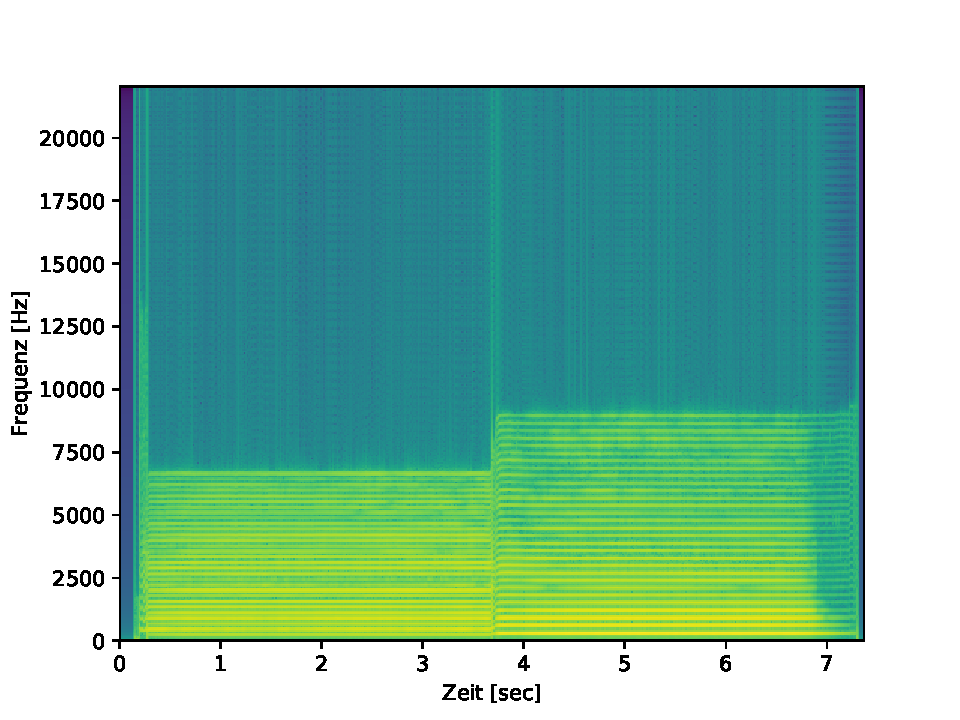
\includegraphics{Figures/buk04_spectrogram}}
    \end{subfigure}%
    \begin{subfigure}{.5\textwidth}
        \centering
        \caption{BuK\_23}
        \scalebox{0.5}{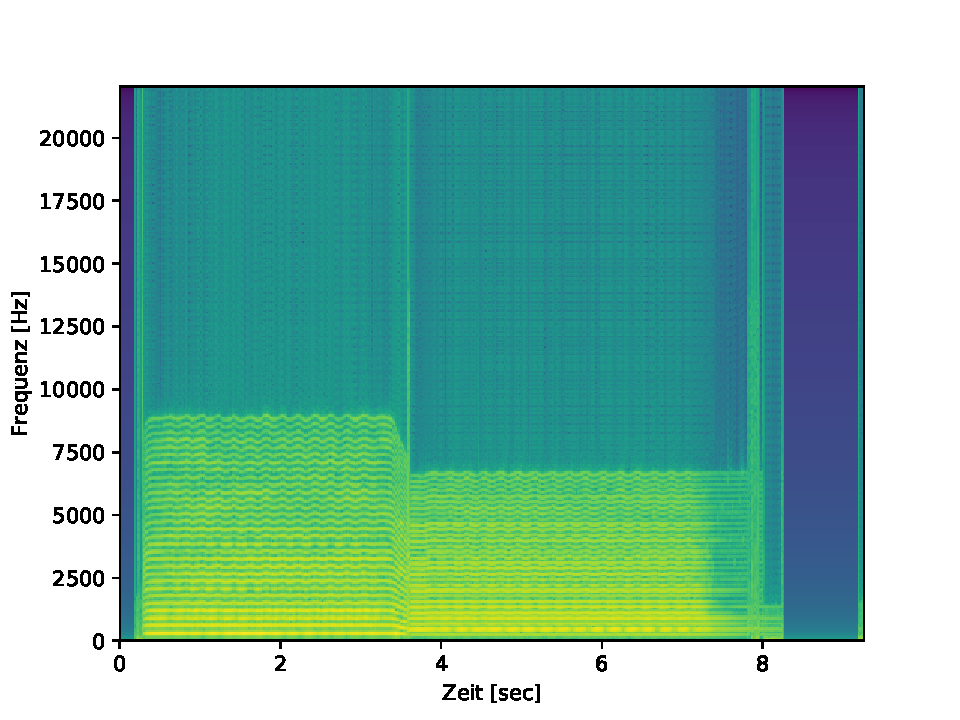
\includegraphics{Figures/buk23_spectrogram}}
    \end{subfigure}
    \caption{Spektrogram der generierten Töne}
    \label{fig:spectrogram}
\end{figure}

\files{main.py}


\section{Freie Harmonische Synthese}
\label{sec:3}


\subsection{}
\files{main.py}


\subsection{}
\files{main.py}


%\section{Berücksuchtugung der originalen Phasen}
%\label{sec:4}